%!TEX TS-program = pdflatex
\documentclass[book,14pt,small,oneside]{ncc}
\usepackage[T2A]{fontenc}
\usepackage[utf8]{inputenc}
\usepackage[english,russian]{babel}
%\usepackage[left=18mm,right=18mm,top=25mm,bottom=20mm]{geometry}
\usepackage[
  a4paper, mag=1000,
  left=2.5cm, right=1cm, top=2cm, bottom=2cm, headsep=0.7cm, footskip=1cm
]{geometry}
\usepackage{nccmath}
\usepackage{amsfonts,amssymb}
\usepackage{hyperref}
\usepackage{nccfancyhdr}
\usepackage[section,above,below]{placeins}
\usepackage{afterpage,flafter}
\usepackage{lastpage}
\usepackage{morefloats}
\usepackage{cite}
\usepackage{float,nccsect}

\usepackage[square,numbers,sort&compress]{natbib}

%\usepackage{xltxtra,xunicode}
%\defaultfontfeatures{Scale=MatchUppercase,Ligatures=TeX}
%\setromanfont[Numbers=Uppercase,Ligatures=TeX]{Arial}
%\setmainlanguage{english}
%\setotherlanguage{russian}

\renewtheorem{theorem}{Теорема}[theorem]

\pagestyle{plain}
%\renewcommand{\headrulewidth}{0pt}
%\lhead{}
%\rhead{\thepage}
%\chead{}
%\lfoot{}
%\rfoot{}
%\cfoot{}

%\DeclareSection*{0}{chapter}{\bf\normalsize}%
%{3.5ex plus 1ex minus .2ex}%
%{2.3ex plus .2ex}{
%\thispagestyle{fancy}
%\bf\normalsize\MakeUppercase}
%
%\DeclareSection*{1}{section}{}%
%{3.5ex plus 1ex minus .2ex}%
%{2.3ex plus .2ex}{\bf\normalsize}

%\newfloat{program}{tp}{lop}[chapter]
%\floatname{program}{Program}
%\RegisterFloatType{program}
%\DeclareSection{-3}{program}{\bff Табл.}{0pt}{0pt}{}
%\DeclareTOCEntry{-3}{}{}{9.9}{}

%\DeclareSection{-2}{table}{}{0pt}{10pt}{}
%\DeclareSection{-1}{figure}{\bff Рис.}{10pt}{0pt}{}
%\DeclareSection{-1}{theorem}{\bff Теорема}{10pt}{0pt}{}

%\NumberlineSuffix{.}{\enskip}

%\SectionTagSuffix{.\quad}

\setcounter{totalnumber}{10}
\setcounter{topnumber}{10}
%\setcounter{page}{1}
\linespread{1.3}

\begin{document}

%\mathversion{bold}
\sectionstyle{center}
\indentaftersection
\sectiontagsuffix{.\;}
%\captiontagsuffix{~---~}

%\setyear{2015}
%\titlehead{Национальный аэрокосмический университет им.~Н.~Е.~Жуковского ``ХАИ''}
%\titlefoot{Харьков~--- \theyear}
%\author{Е.~А.~Танчик}
%\title{Упругая механика многокомпонентных тел}
%\maketitle
\begin{titlepage}
\begin{center}
Национальный аэрокосмический университет им.~Н.~Е.~Жуковского ``ХАИ''
\end{center}
\vskip1cm
\begin{flushright}
На правах рукописи \\
УДК 539.3
\end{flushright}
\vskip2cm
\begin{center}
\large Танчик Евгений Андреевич
\end{center}
\vskip1cm
\begin{center}
\huge\bf Пространственные задачи теории упругости для~некоторых классов неосесимметричных многосвязных тел
\end{center}
\vskip1cm
\begin{center}
01.02.04~--- Механика деформированного твердого тела
\end{center}
\vskip1cm
\begin{center}
ДИССЕРТАЦИЯ \\
на соискание ученой степени \\
кандидата физико-математических наук
\end{center}
\vskip2cm
\begin{flushright}
Научный руководитель \\
д.~ф.-м.~н., проф. \\
Николаев Алексей Георгиевич
\end{flushright}
\vskip2cm
\begin{center}
Харьков~--- 2015
\end{center}
\end{titlepage}
\tableofcontents

%!TeX root = thesis.tex
%!TEX TS-program = pdflatex

\setcounter{secnumdepth}{-1}
\chapter{Введение}
\setcounter{secnumdepth}{2}

{\bf Актуальность темы.} Современный уровень развития техники и технологии в высокотехнологических областях накладывает повышенные требования на точность и эффективность моделей материалов, которые широко используются в авиации и ракетостроении. Одной из наиболее важных характеристик материалов, которые здесь применяются, является такая комплексная характеристика, как малая удельная масса и одновременно высокая прочность материала. Такой характеристикой обладают материалы типа композитов, в которых присутствуют конструктивно заложенные неоднородности. При современном уровне моделирования появляется возможность конструирования материалов с заранее заданными свойствами вначале на уровне модели, определяя оптимальную структуру, геометрические размеры и механические характеристики неоднородностей. И только после этого полученные в результате моделирования данные можно воплощать в реальном материале.

По самому названию композиционный материал~--- это составной материал, обладающий гетерогенной структурой. Разнородные компоненты композита имеют различные физико-механические свойства. Особое сочетание этих свойств и геометрии неоднородностей приводит к качественно новым характеристикам композита, отличным от характеристик составляющих его фаз. Двухфазный композит~--- это однородный материал, армированный волокнами или зернами из другого материала. В зависимости от технологии изготовления армирующие элементы тем или иным способом пропитываются связующим веществом (матрицей), которое после застывания обеспечивает сплошность композиционной среды и идеальный механический и тепловой контакт между разнородными фазами. В качестве армирующих элементов обычно применяют материалы с кристаллической или аморфной микроструктурой, такие, как полимеры, стекла, металлы и др. К материалам заполнителя относятся полимеры, металлы, керамика. Свойства композита существенно зависят от физико-механических характеристик арматуры и матрицы, геометрии арматуры, структуры армирующих элементов, характера их упаковки, объемного содержания элементов, углов армирования и др. Укажем на те основные физико-механические характеристики композиционного материала, которые приводятся в нормативных документах и должны контролироваться в процессе его изготовления. Это модули упругости и пределы прочности на растяжение, сжатие и поперечный сдвиг, коэффициенты Пуассона и линейного температурного расширения вдоль и поперек волокон, удельная теплоемкость и др.{\sloppy\par}

В настоящей работе будут рассмотрены композиционные и пористые материалы, обладающие регулярной структурой. Под регулярной структурой понимается периодическое расположение слоев, зерен или волокон в материале. Считается, что фи\-зи\-ко-\-ме\-ха\-ни\-че\-ские характеристики включений одинаковые, но отличаются от характеристик матрицы. Далее будут рассмотрены только упругие модели деформирования этих материалов.

До настоящего времени многие важные задачи механики композиционных материалов остаются неизученными или недостаточно изученными. К ним относятся задачи определения напряженно-деформированного состояния образца из пористого и композиционного материалов в зависимости от приложенной внешней нагрузки, задачи выявления зон концентрации упругих напряжений как областей, в первую очередь подверженных разрушению, задачи анализа напряжений и деформаций в композиционном материале с отслоившимися включениями, задачи с межфазными и внутрифазными трещинами и др. Актуальной остается задача теоретического определения эффективных упругих модулей композиционных и пористых материалов. Все эти задачи в общей постановке относятся к классу весьма сложных задач механики деформированного твердого тела с многосвязной неоднородной структурой. До последнего времени эффективных методов решения подобных задач не существовало.

{\bf Связь работы с научными программами.} Исследования по теме диссертации проводились в рамках госбюджетной научной темы ``Новые методы исследования линейно и нелинейно деформируемых тел из композиционных материалов'', номер государственной регистрации № 0112U002135. 

{\bf Цель и задачи исследования.} Целью исследования является развитие обобщенного метода Фурье на решение неосесимметричных многосвязных задач теории упругости с большим числом компонент связности для канонических тел, ограниченных поверхностями цилиндра, сферы, вытянутого и сжатого сфероидов. 

{\it Объектом исследования} являются изотропные упругие тела под действием одноосного и двуосного растяжения.

{\it Предметом исследования} является неосесимметричное напряженное состояние многосвязных или гетерогенных тел.

{\it Методы исследования.} Для достижения поставленной цели в работе развит обобщенный метод Фурье, получены теоремы сложения (переразложения) для модифицированных базисных частных решений уравнения Ламе для сферы, вытянутого и сжатого сфероидов. Данные теоремы позволяют представить общее решение задачи в системе координат, связанной с каждой из граничных поверхностей и обеспечить точное удовлетворение граничных условий.

{\bf Научная новизна полученных результатов} состоит в развитии обобщенного метода Фурье для решения неосесимметричных многосвязных задач теории упругости для канонических тел, ограниченных координатными поверхностями цилиндра, сферы, вытянутого и сжатого сфероидов.

{\bf Практическое значение полученных результатов} состоит в том, что развитый в диссертации метод позволяет вычислять на\-пряжен\-но-де\-форми\-ро\-ван\-ное состояние в любых неосесимметричных телах описанной геометрии с большим числом компонент связности под действием одноосного, двуосного или всестороннего растяжения или сжатия упругого пространства.

Полученные результаты также использованы для вычисления упругих модулей пористых и зернистых композиционных материалов.

{\bf Личный вклад соискателя.} Основные результаты получены соискателем самостоятельно.

{\bf Апробация результатов диссертации.} Основные результаты исследований докладывались и обговаривались на VIII и IX международных научных конференциях ``Математические проблемы механики неоднородных структур'' (Львов, 2010, 2014), ``Современные проблемы механики деформируемого твердого тела, дифференциальных и интегральных уравнений'' (Одесса, 2013), международной математической конференции им.~В.~Я.~Скоробогатька (Дрогобыч, 2011), XVI International Conference ``Dynamical System Modelling  and Stability Investigation'' (Киев, 2013), (Запорожье, 2012), ``Человек и Космос'' (Днепропетровск, 2010), ``Интегрированные компьютерные технологии в машиностроении'' (Харьков, 2010).

{\bf Публикации.} Основные научные результаты опубликованы в 21 статьях в научных журналах и сборниках трудов, которые соответствуют требованиям ВАК Украины к опубликованию результатов диссертации в профильных изданиях. 

{\bf Структура работы.} Диссертация состоит из вступления, 4 глав, выводов, списка литературы из 140 наименований. Общий объем работы~--- N страниц.

{\bf Обзор литературы.} Приведем обзор научных исследований, связанных с тематикой данной работы. Исследованию пространственных задач теории упругости для односвязных цилиндра, шара и сфероида посвящены работы~\cite{Abramian, Andreev, Valov, Volpert1977, Volpert1967, Gomilko, Grinchenko1965, Grinchenko1967, Grinchenko1985, Grinchenko1978, Lur'e, Podilchuk1967, Podilchuk1984, Prokopov, Tokovyy, Ulitko, Chen1978-1, Chen1978-2, Edwards, Zhong, Zureick1989, Zureick1988, Ambartsumian, Arutynian, Kaufman, Kolesov, Meleshko}. В них краевые задачи для указанных областей решены методом Фурье.

В работах А.~Я.~Александрова~\cite{Aleksandrov1978, Aleksandrov1973} получил развитие метод интегральных наложений, позволивший связать пространственное напряженное состояние с плоским и, как следствие, выразить решения ряда пространственных задач для односвязных и многосвязных тел через аналитические функции комплексного переменного.

Г.~Н.~Положий на основе построенной им теории р–аналитических функций предложил метод решения осесимметричных задач теории упругости, аналогичный методу Колосова~--- Мусхелишвили для плоских задач. В дальнейшем этот метод был распространен на двусвязные тела в работах А.~А.~Капшивого, Л.~Н.~Ломоноса~\cite{Kapshiviy, Lomonos}.

Важный подход к решению пространственных задач теории упругости основан на применении методов теории потенциала. В работах В.~Д.~Купрадзе, Т.~Г.~Гегели, О.~М.~Башелейшвили, Т.~В.~Бурчуладзе~\cite{Kupradze, Burchuladze} путём исследования сингулярных интегральных уравнений различных классов краевых задач теории упругости были установлены условия существования и единственности их решений. Параллельно были созданы алгоритмы численного решения задач методами теории потенциала~\cite{Aleksandrov1973}. Численные возможности трех последних методов в многосвязных неосесимметричных телах весьма ограничены.
 
Методы теории потенциала в простанственных задачах теории трещин были развиты в монографии~\cite{Kit}.
  
В монографии~\cite{Guz1984} описан метод решения краевых задач теории упругости для областей, близких к каноническим, путем возмущения формы границы.

Приведем анализ методов решения пространственных задач для многосвязных тел. Прежде всего, заметим, что в этой области отсутствуют методы, близкие по общности и эффективности к методам решения плоских задач. Используемые здесь методы либо носят частный характер и предназначены для областей специального вида, не допуская распространения на более сложные области, либо, в виду своей общности, недостаточно эффективны при решении конкретных задач~\cite{Chen1978-2, Miyamoto, Sheikh, Strenberg}.

Многие задачи решаются численными методами~\cite{Method, Erzhanov}. Однако в телах с большим количеством неоднородностей эти методы неэффективны.

Остановимся на методах исследования механики композиционных материалов. Определение интегральных упругих характеристик композиционных материалов проводилось различными методами в работах: Н.~С.~Бахвалова~\cite{Bahvalov}, Л.~Браутмана~\cite{Brautman}, А.~С.~Вавакина~\cite{Vavakin}, Ван Фо Фы~\cite{VanFoFiKo1971, VanFoFi1971}, Г.~А.~Ванина~\cite{Vanin1985, Vanin1994, Vanin1976, Vanin1980, Vanin1977}, А.~Н.~Власова, О.~К.~Гаришина~\cite{Garishin}, А.~В.~Головина, В.~Т.~Головчана~\cite{Golovchan1974, Golovchan1993, Golovchan1987, Golovchan2000}, В.~Т.~Гринченко~\cite{Grinchenko1965, Grinchenko1967, Grinchenko1985, Grinchenko1978}, А.~Н.~Гузя~\cite{Guz1968}, А.~В.~Дыскина~\cite{Diskin}, А.~В.~Ефименко, С.~П.~Киселёва, С.~П.~Копысова, Р.~Кристенсен~\cite{Kristensen}, Г.~Н.~Кувыркина, В.~И.~Куща~\cite{Kusch1995}, В.~М.~Левина~\cite{Levin}, Б.~П.~Маслова, В.~В.~Мошева, А.~А.~Панькова, Б.~Е.~Победри~\cite{Pobedrya}, Ю.~Н.~Подильчука~\cite{Podilchuk1967, Podilchuk1984}, В.~В.~Полякова, Я.~Я.~Рущицкого, Р.~Л.~Салганик~\cite{Salganik}, К.~Б.~Устинова~\cite{Ustinov}, А.~Ф.~Федотова~\cite{Fedotov}, В.~М.~Фомина, Л.~П.~Хорошуна~\cite{Khoroshun, Khoroshun2000-1, Khoroshun2000-2}, Т.~Д.~Шермергора~\cite{Schermergor}, Дж.~Эшелби~\cite{Eshelbi, Eshelby}, B.~Budiansky~\cite{Budiansky}, S.~Boucher~\cite{Boucher}, R.~M.~Christensen~\cite{Christensen, Christensen1990}, Z.~Hashin~\cite{Hashin, Hashin1983, Hashin1988, Hashin1963}, M.~Kachanov~\cite{Kachanov}, S.~Nemat-Nasser, M.~Taya~\cite{Nemat-Nasser}, A.~S.~Sangini, W.~Lu~\cite{Sangini}, S.~Torquato~\cite{Torquato}, R.~W.~Zimmerman~\cite{Zimmerman} и др.{\sloppy\par}

Один из первых подходов к определению эффективных упругих модулей был предложен в работах Дж.~Эшелби~\cite{Eshelbi, Eshelby}. Он основан на решении задачи об одиночном включении в форме эллипсоида. Метод предполагает пренебрежение взаимодействием между включениями.

В работе~\cite{Kachanov} при анализе эффективных упругих свойств тела с трещинами использовался метод эффективного поля, в котором предполагается, что включения находятся в поле напряжений, соответствующему среднему полю напряжений в матрице.

В ряде работ~\cite{Christensen1990} использовался метод самосогласования, в котором каждое включение находится в эквивалентной упругой среде, соответствующей матрице и остальным включениям, а также дифференциальный вариант метода самосогласования~\cite{Salganik, Vavakin, Zimmerman}.

В работе~\cite{Fedotov} предложен метод расчета эффективных упругих модулей зернистых композитов, основанный на модели упругого деформирования пористых материалов. Отличительная особенность метода заключается в осреднении микроскопических напряжений и деформаций не по полному, а по эффективному объему фаз. Получены расчетные зависимости эффективных объемов осреднения от упругих модулей и объемного содержания фаз. Проведено сопоставление результатов расчета с экспериментальными данными при различном сочетании упругих модулей и произвольной объемной концентрации фаз.

Модели многослойных материалов и конструкций исследовались в монографии~\cite{Bolotin}.

В книге~\cite{Gerega} рассматривается моделирование перколяционных кластеров фаз внутренних границ композиционных материалов.

В монографиях~\cite{Grigoliuk, Savin} решаются плоские задачи для многосвязных тел с отверстиями.

В книге~\cite{Erzhanov} метод конечных элементов применен при анализе напряжений в двухсвязных телах.

В статье~\cite{Zharkov} исследовано напряженно-деформированное состояние дисперсно наполненного полимерного композита с использованием объемных моделей.

В статьях~\cite{Khoroshun2000-1, Khoroshun2000-2, Scalon, Trias} обобщены базовые подходы, применяемые в математических моделях, и общие методы решения уравнений механики стохастических композитов. Они могут быть сведены к стохастическим уравнениям теории упругости структурно неоднородного тела, к уравнениям теории эффективных упругих модулей, к уравнениям теории упругих смесей или к более общим уравнениям четвертого порядка. Решение стохастических уравнений теории упругости для произвольной области вызывает значительные математические трудности и может быть реализовано только приближенно. Построение уравнений теории эффективных упругих модулей связано с задачей определения интегральных модулей стохастически неоднородной среды, которая может быть решена методом возмущений, методом моментов или методом условных моментов. Однако поскольку уравнения состояния не были строго обоснованы, эта теория не может использоваться для систематического моделирования композитных структур.

В работе~\cite{Golovchan2000} проанализировано термонапряженное состояние в окрестности сферических включений в   керамическом композите. Была строго решена краевая задача, которая соответствует приближенному моделированию механики композита парой включений. Численные результаты качественно согласуются с известными экспериментальными зависимостями.

В статье~\cite{Zureick1988} получено явное аналитическое решение задачи с жестким сфероидальным включением в трансверсально изотропном упругом пространстве, где включению заданы контактные перемещения в направлении, перпендикулярном к оси симметрии материала. Для решения задачи использовано представление потенциала перемещений для равновесия трехмерного трансверсально изотропного тела.

В работе~\cite{Zhong} исследован трансверсально изотропный стержень с цилиндрическим включением с осесимметричными собственными деформациями. Получено аналитическое упругое решение для перемещений, напряжений и энергии упругой деформации стержня.

В монографии~\cite{Vanin1985} разработаны методы микромеханики композиционных сред с дискретной структурой и трещинами и некоторые их приложения к конкретным материалам. Рассмотрено влияние свойств компонентов и вида структуры неоднородных сред на их эффективные (интегральные) параметры и распределение внутренних полей. Наряду с задачами теории упругости исследуются другие физические свойства материалов.

%В статье~\cite{Garishin} предложена структурная модель зернистого эластомерного композита, позволившая связать его деформационное и прочностное поведение с размерами частиц дисперсной фазы, т.~е. учесть масштабный фактор прочности. На основе теоретических исследований на\-пря\-жен\-но-де\-фор\-ми\-ро\-ван\-но\-го состояния вокруг двух жестких сферических включений в упругой несжимаемой матрице установлены зависимости математического ожидания разрывного усилия от физико-механических характеристик связующего, размеров частиц и расстояния между ними. В результате предложен новый вероятностный критерий появления микроразрушения в композитной структуре в виде отслоений матрицы от частиц. С его помощью проведены модельные исследования процессов развития внутренней поврежденности в композитной системе в зависимости от степени наполнения и величины включений. Построены соответствующие кривые растяжения, определены предельные разрывные макронапряжения и макродеформации.

В работе~\cite{Shailiev} построена математическая модель расчета эффективного модуля упругости полиминеральных горных пород. Суть исследований заключается в расчете эффективного упругого модуля характерного объема материала путем осреднения по всем реализациям случайного поля неоднородностей с учетом их концентрации и пространственной ориентации. В работе были использованы методы: теории обобщенных функций, тензорного исчисления, теории уравнений математической физики и ин\-тег\-ро-\-диф\-фе\-рен\-ци\-аль\-ных уравнений.

В работе~\cite{Dudchenko} дано построение модели межфазного слоя материала, содержащего жесткую частицу под действием растягивающей нагрузки. Предлагается вариант чисто конструктивной расчетной модели. Основанием для построения такой модели являются результаты исследований, где показано, что в окрестности границ включения возникает дополнительная межфазная зона, механические свойства которой являются переменными, изменяясь по экспоненциальному закону от жесткости включения до жесткости матрицы. В рамках полученной расчетной модели учитываются размеры включения и протяженность межфазной зоны. Учитываются также изменение модулей упругости при повороте частицы по отношению к действующей нагрузке и влияние соседних частиц на свойства межфазного слоя. Приведены примеры расчета.

%В статье~\cite{Chernous} представлены исследования по моделированию структуры пористых материалов с малой объемной долей содержания твердой фазы. В качестве моделей рассматриваются главным образом стержневые и оболочечные конструкции. Предложена классификация моделей по степени упорядоченности структурных единиц. Представляется, что наиболее адекватной с точки зрения морфологии и деформационных свойств является модель, состоящая из хаотически ориентированных 14-гранных ячеек. Для анализа представленной модели предлагается метод выделения структурного элемента.

В работе~\cite{Akbarov} методом конечных элементов исследовано влияние начального растяжения на концентрацию напряжений вокруг круговых отверстий в пластине-полосе, подверженной изгибу. Математическая формулировка соответствующей краевой задачи дается в рамках трехмерной линеаризованной теории упругости при плоском деформированном состоянии. Материал пластины-полосы~--- линейно-упругий, однородный и ортотропный. Представлены численные результаты, оценивающие влияние предварительного растяжения и взаимного расположения отверстий на концентрацию напряжений. Установлено, что начальное растяжение существенно уменьшает концентрацию напряжений в некоторых характерных точках на контуре отверстий.

В статье~\cite{Yankovskiy} разработана численно-аналитическая методика моделирования нелинейно-наследственного поведения композитов, имеющих про\-стран\-ст\-ве\-н\-но-ори\-ен\-ти\-ро\-ва\-н\-ную структуру (пространственно-армированных композитов), позволяющая в дискретные моменты времени рассматривать такую композицию как не\-ли\-ней\-но-уп\-ру\-гую. Применение итерационного процесса типа метода переменных параметров упругости позволило линеаризовать определяющие соотношения и свести задачу расчета механического поведения рассматриваемого композита в дискретные моменты времени к серии ли\-ней\-но-уп\-ру\-гих задач механики композитов. 

%В статье~\cite{Golotina} исследованы зернистые композитные материалы с эластомерной матрицей, наполненной твердыми частицами диаметром $10-1000~\text{мкм}$. Рассмотрен один из возможных механизмов реологического поведения наполненных систем, связанный с возникновением и развитием вакуолей около жестких включений в вязкоупругой матрице. Для моделирования такого механизма формирования реологических свойств наполненного эластомера использована структурная ячейка в виде эластомерного цилиндра, высота которого равна диаметру, с жестким сферическим включением в центре цилиндра. Деформирование ячеек исследовали при соблюдении граничных условий, обеспечивающих сохранение их плотной упаковки при деформировании. Принято, что включение является жестким, а свойства матрицы описываются уравнениями линейной наследственной теории вязкоупругости. Для описания процесса роста вакуоли использован подход, согласно которому изначальное отслоение начинает распространяться, когда энергия, накопленная в матрице при растяжении, достигает величины, достаточной для создания новой поверхности раздела. Структурную неоднородность композита моделировали путем учета непостоянства локальной концентрации наполнителя. Рассчитаны кривые ползучести для композитов с разным содержанием твердой фазы. Проведено сравнение с экспериментальными данными, показавшее удовлетворительное согласование результатов.{\sloppy\par}

%В работе~\cite{Gordeev} предлагается алгоритм оценки свойств волокнистого композита при растяжении, основанный на процедуре В.~З.~Власова; дается оценка эффективных свойств эквивалентного гомогенного материала; приводится сравнение результатов расчета эффективного модуля Юнга с результатами других авторов.

В статье~\cite{Belov} предлагается корректная модель сред с микроструктурой (по определению Миндлина), которая определяется наличием свободных деформаций и обобщает известные модели Миндлина, Коссера и Аэро-Кувшинского. Корректность формулировки модели определяется использованием ``кинематического'' вариационного принципа, основанного на последовательном формальном описании кинематики сред, формулировке кинематических связей для сред разной сложности и построении соответствующей потенциальной энергии деформации с использованием процедуры множителей Лагранжа. Ус\-та\-нав\-ли\-ва\-ет\-ся система определяющих соотношений и формулируется согласованная постановка краевой задачи. Показывается, что исследуемая модель среды не только отражает масштабные эффекты, аналогичные когезионным взаимодействиям, но и является основой для описания широкого спектра адгезионных взаимодействий. В связи с анализом физической стороны модели предлагается трактовка физических характеристик, ответственных за неклассические эффекты, дается описание спектра адгезионных механических параметров.

В работе~\cite{Garishin} разработаны модели структур многоуровневых волокнистых композитов с упрочняющими частицами в матрице и методы решения задач о плоском напряженном состоянии и разрушении. Предложен новый критерий хрупкого разрушения на основе интегралов, не зависящих от пути интегрирования. Найдены обобщенные равновесные термодинамические потенциалы неоднородных сред. Предложены методы определения поправок в состоянии материалов, возникающих от градиентных эффектов вблизи свободных и межфазных поверхностей, кончиков трещин, при высокочастотных волновых процессах. Указанные результаты оригинальны, и пока не известны их аналоги в литературе. Соотношения теории описывают состояние тел на выбранном масштабном уровне и связывают его с состоянием и процессами, протекающими на других масштабных уровнях неоднородных сред. Отмеченное представляет интерес в теории разрушения материалов, в задачах нанотехнологии и др.

Исследование напряженного состояния тела с однопериодической системой сферических полостей (осесимметричная задача) проводилось в работе~\cite{Olegin}.

Двусвязные осесимметричные задачи рассмотрены в работах~\cite{Smirnov, Atsumi, Mura, Tsuchida1980, Tsuchida1979}. Напряженно-деформированное состояние кусочно-однородных тел исследовано с помощью обобщенного метода Фурье в работах~\cite{Nikolaev2003, Nikolaev2004, Nikolaev2011, Nikolaev2007, Nikolaev2010, Nikolaev2009, Nikolaev2013, Nikolaev2012, Nikolaev-Tanchik2012, Nikolaev2013-1, Nikolaev2013-2, Nikolaev2013-19, Nikolaev2013-4, Nikolaev2014-1, Nikolaev2014-9, Nikolaev2013-3, Nikolaev2014-2, Nikolaev2014-3, Nikolaev2014-4, Nikolaev2014-5, Nikolaev2014-6, Nikolaev2014-7, Nikolaev2015-1}.
%Аппарат обобщенного метода Фурье развит в работах~\cite{Nikolaev1984, Nikolaev2011, Nikolaev1993, Nikolaev1998, Nikolaev1998-1}.

Приведенный обзор литературы показывает, что одной из актуальных проблем современной механики деформированного твердого тела является построение и анализ моделей напряженного состояния пористых и композиционных материалов, которые находят широкое применение в высокотехнологических областях техники, в частности в авиации и ракетостроении. Известные пространственные модели напряженного состояния указанных выше материалов не являются достаточно точными. Они учитывают неоднородную структуру материала или усредненно, или локально в окрестности только одного концентратора напряжений. При моделировании подобных материалов также используются разные типы стохастических моделей, которые, как правило, не являются полностью адекватными. Однако аэрокосмическая отрасль накладывает повышенные требования на прочностные характеристики материалов, управление которыми зависит от точности определения напряжений в теле. Создание более точных моделей указанных материалов позволит не только уточнить расчеты на прочность (коэффициенты концентрации напряжений на границе раздела фаз могут отличаться в 1.5--2 раза), но и на основе этих моделей проводить оптимальное проектирование материалов с заданными прочностью и массой. Обзор литературы показывает, что напряженное состояние в пористом и композиционном материалах традиционно моделируется напряженным состоянием представительской ячейки, содержащей одну неоднородность. Подобные модели используются при определении эффективных упругих модулей материалов с порами и включениями. Очевидно, эти модели заведомо не обладают высокой точностью. Основным их недостатком является тот факт, что они не вполне адекватны в локальных зонах концентрации напряжений в телах из пористых и композиционных материалов.

В диссертации приводятся результаты исследований по моделированию на\-пря\-же\-н\-но-де\-фор\-ми\-ро\-ва\-н\-но\-го состояния упругого пористого и композиционного материалов с порами или включениями цилиндрической, сферической, вытянутой или сжатой сфероидальной формы. Пористый или композиционный материал моделируется упругой средой с конечным числом полостей или включений указанной выше формы. Число неоднородностей варьируется в широком диапазоне (от 2 до 30). 
%Также рассматриваются задачи для упругого пространства с бесконечным числом полостей или включений, образующих периодическую структуру.
%Объектом исследования настоящей работы является многосвязный кусочно-однородный упругий материал. Предметом исследования являются модели НДС многосвязного кусочно-однородного упругого материала. Целью и задачами данного исследования является построение ана\-ли\-ти\-ко-чис\-ле\-н\-ных моделей НДС упругих тел с полостями и включениями, указанной выше формы.
%Важной составной частью исследования является строгий анализ полученных моделей, определение областей их эффективности, численный анализ полей напряжений и деформаций на основе построенных моделей, проверка адекватности предлагаемых моделей.
Модели НДС указанных тел строятся на основе точных базисных решений уравнения Ламе в канонических пространственных областях~\cite{Nikolaev1993, Nikolaev1998, Nikolaev1984}. Для определения параметров модели используется обобщенный метод Фурье. Аппарат обобщенного метода Фурье был развит в работах~\cite{Nikolaev1998, Nikolaev2011, Nikolaev1998-1, Nikolaev1993, Nikolaev1984}.

Остановимся кратко на содержании диссертации.

В главе 1 приведен аппарат обобщенного метода Фурье. Кроме известных теорем сложения базисных решений уравнения Ламе в цилиндрических, сферических, вытянутых и сжатых сфероидальных системах координат, начала которых произвольно сдвинуты друг относительно друга, впервые получены теоремы сложения для модифицированных базисных решений уравнения Ламе в указанных системах координат. Эти теоремы впервые были получены в работах~\cite{Nikolaev2014-1, Nikolaev2014-9}.

В главе 2 исследована механика упругого деформирования волокнистых пористых и композиционных материалов. Волокна моделируются параллельно расположенными цилиндрическими полостями или включениями. Рассмотрены локальные модели, в которых напряженно-деформированное состояние определяется цилиндрической неоднородностью и ее ближайшими соседями. Изучены также глобальные модели, которые учитывают всю структуру материала. Основное внимание уделяется количественному и качественному анализу в распределении напряжений в представительской ячейке в зависимости от механических и геометрических характеристик матрицы и включений, а также от типа упаковки полостей или включений. Приведены сравнения разных типов моделей. Результаты этой главы получены в работах~\cite{Nikolaev2013-1, Nikolaev2013-2, Nikolaev2013-4, Nikolaev2013-3, Nikolaev2015-1}.
 
Глава 3 посвящена механике упругого деформирования зернистых композиционных и пористых материалов со сферическими зернами. Рассмотрены локальные модели, в которых напряженно-деформированное состояние определяется сферической неоднородностью и ее ближайшими соседями. Изучены также глобальные модели, которые учитывают всю структуру материала. Основное внимание уделяется количественному и качественному анализу в распределении напряжений в представительской ячейке в зависимости от механических и геометрических характеристик матрицы и включений, а также от типа упаковки полостей или включений. Рассмотрены тетрагональная и гексагональная типы упаковок неоднородностей в случаях отсутствия или наличия объемного центрирования.
Приведены сравнения этих типов моделей. Результаты этой главы получены в работах~\cite{Nikolaev2012, Nikolaev2014-2, Nikolaev2014-5, Nikolaev2014-7}.

В главе 4 рассмотрены модели упругого деформирования пористых и композиционных материалов с вытянутыми сфероидальными полостями или включениями. Указанные материалы моделируются упругим пространством с конечным или бесконечным числом неоднородностей, центры которых расположены в узлах периодической решетки, обладающей определенной трансляционной симметрией. Предполагается, что оси симметрии включений одинаково направлены. Рассмотрены локальные модели, в которых на\-пряжен\-но-де\-форми\-ро\-ван\-ное состояние определяется неоднородностью и ее ближайшими соседями. Изучены также глобальные модели, которые учитывают всю структуру материала. Приведен количественный и качественный анализ распределения напряжений в представительской ячейке в зависимости от механических и геометрических характеристик матрицы и включений, а также от типа упаковки неоднородностей. Рассмотрены тетрагональная и гексагональная типы упаковок неоднородностей в случаях отсутствия или наличия объемного центрирования.
Приведены сравнения этих типов моделей. Результаты этой главы получены в работах~\cite{Nikolaev2010, Nikolaev-Tanchik2012, Nikolaev2013, Nikolaev2014-1, Nikolaev2014-9, Nikolaev2014-3, Nikolaev2014-4, Nikolaev2014-6}.

%В главе 6 изучены краевые задачи для уравнения Ламе в областях с бесконечным числом полостей или включений, которые образуют периодическую структуру. Рассмотрено пространство с полостями или включениями в форме сфер, вытянутых или сжатых сфероидов под действием одноосного, двуосного или всестороннего растяжений, приложенных на бесконечности. Приведен анализ распределения напряжений в представительской ячейке в зависимости от механических и геометрических характеристик матрицы и включений. Дано сравнение напряжений для разных типов моделей (локальные, глобальные и периодические).
%
%Глава 7 посвящена определению эффективных упругих модулей некоторых типов пористых и композиционных материалов. 
 
%В рамках второго этапа бюджетной темы были построены и исследованы глобальные модели НДС в телах с неоднородностями, которые описывают поля напряжений и деформаций реального пористого или композиционного материала в зависимости от типа упаковки неоднородностей и их числа в упругом теле. Проведен строгий аналитический анализ построенных моделей и определены области их эффективности. Созданы пакеты прикладных программ для численной реализации построенных моделей. Проведен численный и качественный анализ распределения напряжений в некоторых рассматриваемых телах. Дано сравнение изученных глобальных моделей с локальными моделями, исследованными на первом этапе бюджетной темы. Результаты исследований приведены в работах~\cite{Nikolaev2013-1, Nikolaev2013-2, Nikolaev2013-3, Nikolaev2013-4, Nikolaev2013-5, Nikolaev2013-6, Nikolaev2013-7, Nikolaev2013-8, Nikolaev2013-9, Nikolaev2013-19}.

%Они докладывались на международных конференциях~\cite{Tanchik, Nikolaev2013-10, Nikolaev2013-11, Nikolaev2013-12, Nikolaev2013-13, Nikolaev2013-14, Nikolaev2013-15, Nikolaev2013-16, Nikolaev2013-17, Nikolaev2013-18}.
%!TeX root = thesis.tex
%!TEX TS-program = pdflatex

\chapter{Математический аппарат обобщенного метода Фурье}

\section{Теоремы сложения базисных гармонических функций в~цилиндрических, сферических, вытянутых и сжатых сфероидальных системах координат со сдвинутыми началами}

Рассмотрим пары $(i = 1,2)$ однотипных одинаково направленных систем координат: декартовых $\left( {{x_i},{y_i},{z_i}} \right)$, цилиндрических $\left( {{\rho _i},{z_i},{\varphi _i}} \right)$, сферических $\left( {{r_i},{\theta _i},{\varphi _i}} \right)$, вытянутых $\left( {{\xi _i},{\eta _i},{\varphi _i}} \right)$ и сжатых $\left( {{{\tilde \xi }_i},{{\tilde \eta }_i},{\varphi _i}} \right)$ сфероидальных. Их начала отнесены к точкам ${O_i}$, которые произвольно сдвинуты друг относительно друга. Будем считать, что декартовые координаты точки ${O_2}$ в декартовой системе координат с началом в точке ${O_1}$ задаются тройкой чисел $\left( {{x_{12}},{y_{12}},{z_{12}}} \right)$. Тогда между декартовыми координатами справедливы соотношения\sloppy
\begin{equation}\label{eq:1:1}
\left\{ {\begin{array}{*{20}{l}}
{{x_1} = {x_2} + {x_{12}},}\\
{{y_1} = {y_2} + {y_{12}},}\\
{{z_1} = {z_2} + {z_{12}}.}
\end{array}} \right.
\end{equation}
%\begin{figure}
%\centering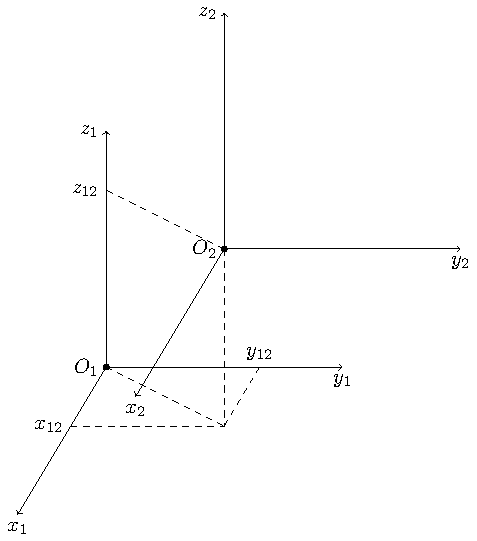
\includegraphics[width=8cm]{cartesian.pdf}
%\caption{Декартовые системы координат, произвольно сдвинутые друг относительно друга}
%\end{figure}
Связь между различными криволинейными координатами определяется формулами:
\begin{equation*}
{x_i} = {\rho _i}\cos {\varphi _i} = {r_i}\sin {\theta _i}\cos {\varphi _i} = {c_i}{\mathop{\rm sh}\nolimits} {\xi _i}\sin {\eta _i}\cos {\varphi _i} = {\tilde c_i}{\mathop{\rm ch}\nolimits} {\tilde \xi _i}\sin {\tilde \eta _i}\cos {\varphi _i},
\end{equation*}
\begin{equation*}
{y_i} = {\rho _i}\sin {\varphi _i} = {r_i}\sin {\theta _i}\sin {\varphi _i} = {c_i}{\mathop{\rm sh}\nolimits} {\xi _i}\sin {\eta _i}\sin {\varphi _i} = {\tilde c_i}{\mathop{\rm ch}\nolimits} {\tilde \xi _i}\sin {\tilde \eta _i}\sin {\varphi _i},
\end{equation*}
\begin{equation}\label{eq:1:2}
{z_i} = {r_i}\cos {\theta _i} = {c_i}{\mathop{\rm ch}\nolimits} {\xi _i}\cos {\eta _i} = {\tilde c_i}{\mathop{\rm sh}\nolimits} {\tilde \xi _i}\cos {\tilde \eta _i},
\end{equation}
\noindent где ${x_i},{y_i},{z_i} \in \left( { - \infty ;\infty } \right)$; ${\rho _i},{r_i},{\xi _i} \in \left[ {\left. {0;\infty } \right)} \right.$; ${\eta _i} \in \left[ {0;\pi } \right]$; ${\tilde \xi _i} \in \left( { - \infty ,\infty } \right)$; ${\tilde \eta _i} \in \left[ {0;\dfrac{\pi }{2}} \right]$; $\varphi  \in \left[ {0;2\pi } \right]$; ${c_i},{\tilde c_i}$ $\left( {{c_i},{{\tilde c}_i} > 0} \right)$~--- параметры сфероидальных систем координат.

В дальнейшем понадобятся базисные решения уравнения Лапласа

\begin{equation}
\Delta u = 0,
\end{equation}
\noindent регулярные вне (знак ``+'' в верхнем индексе), внутри (знак ``--'' в верхнем индексе) цилиндра $\Omega _3^ \pm$, шара $\Omega _4^ \pm$, вытянутого $\Omega _5^ \pm $ и сжатого $\Omega _6^ \pm $ сфероидов:

\begin{equation}\label{eq:1:4}
u_{\lambda ,m}^{ \pm (3)}\left( {\rho ,z,\varphi } \right) = {e^{i\lambda z + im\varphi }}\left\{ \begin{array}{l}
{{\tilde K}_m}\left( {\lambda \rho } \right)\\
{I_m}\left( {\lambda \rho } \right)
\end{array} \right\},\qquad {\kern 1pt} \lambda  \in \mathbb{R},\quad m \in \mathbb{Z};
\end{equation}

\begin{equation}\label{eq:1:5}
u_{n,m}^{ \pm (4)}\left( {r,\theta ,\varphi } \right) = \left\{ \begin{array}{l}
(n - m)!/{r^{n + 1}}\\
{r^n}/(n + m)!
\end{array} \right\}P_n^m(\cos \theta ){e^{im\varphi }};
\end{equation}
$$
n,m \in \mathbb{Z}, n\ge 0, |m| \le n;
$$
\begin{equation}\label{eq:1:6}
u_{n,m}^{ \pm (5)}\left( {\xi ,\eta ,\varphi } \right) = \left\{ \begin{array}{l}
Q_n^{ - m}({\mathop{\rm ch}\nolimits} \xi )\\
P_n^{ - m}({\mathop{\rm ch}\nolimits} \xi )
\end{array} \right\}P_n^m(\cos \eta ){e^{im\varphi }};
\end{equation}
$$
n,m \in \mathbb{Z}, n\ge 0, |m| \le n;
$$
\begin{equation}\label{eq:1:7}
u_{n,m}^{ \pm (6)}\left( {\tilde \xi ,\tilde \eta ,\varphi } \right) = \left\{ \begin{array}{l}
Q_n^{ - m}(i{\mathop{\rm sh}\nolimits} \tilde \xi )\\
P_n^{ - m}(i{\mathop{\rm sh}\nolimits} \tilde \xi )
\end{array} \right\}P_n^m(\cos \tilde \eta ){e^{im\varphi }};
\end{equation}
$$
n,m \in \mathbb{Z}, n\ge 0, |m| \le n;
$$
\noindent где ${I_m}(x)$~--- модифицированная функция Бесселя, $${\tilde K_m}(x) = {({\rm{sign}}{\mkern 1mu} {\kern 1pt} x)^m}{K_m}\left( {|x|} \right),$$
${K_m}(x)$~--- функция Макдональда, $P_n^m(x)$, $Q_n^m(x)$~--- функции Лежандра первого и второго рода. Верхний (нижний) множитель в фигурных скобках соответствует верхнему (нижнему) знаку индекса $\left\{  \pm  \right\}$.

В дальнейшем важную роль играют теоремы сложения решений~\eqref{eq:1:4}~-- \eqref{eq:1:7} в парах однотипных систем координат, описанных выше.

\begin{theorem}
При ${\rho _2} < {\rho _{12}}$ справедливо разложение
\begin{equation}\label{eq:1:8}
u_{\lambda ,m}^{ + (3)}\left( {{\rho _1},{z_1},{\varphi _1}} \right) = \sum\limits_{l =  - \infty }^\infty  {{{( - 1)}^l}} u_{m - l,\lambda }^{ + (3)}\left( {{\rho _{12}},{z_{12}},{\varphi _{12}}} \right)u_{l,\lambda }^{ - (3)}\left( {{\rho _2},{z_2},{\varphi _2}} \right).
\end{equation}

При ${\rho _1} < {\rho _{12}}$ справедливо разложение
\begin{equation}\label{eq:1:9}
u_{\lambda ,m}^{ + (3)}\left( {{\rho _2},{z_2},{\varphi _2}} \right) = \sum\limits_{l =  - \infty }^\infty  {{{( - 1)}^m}} u_{m - l,\lambda }^{ + (3)}\left( {{\rho _{12}}, - {z_{12}},{\varphi _{12}}} \right)u_{l,\lambda }^{ - (3)}\left( {{\rho _1},{z_1},{\varphi _1}} \right).
\end{equation}
\end{theorem}
%\begin{proof}
%Рассмотрим интегральное представление функции~\cite{Nikolaev1998-1}
%
%\begin{equation}\label{eq:1:10}
%u_{\lambda ,m}^{ + (3)}\left( {{\rho _1},{z_1},{\varphi _1}} \right) = {({\rm{sign}}{\mkern 1mu} {\kern 1pt} \lambda )^m}\frac{1}{2}\int\limits_{ - \infty }^\infty  {{e^{|\lambda |\left[ {i{z_1} - {\rho _1}{\mathop{\rm ch}\nolimits} (t - i{\varphi _1})} \right] + mt}}} dt,
%\end{equation}
%
%$\lambda  \ne 0$, ${\rho _1} > 0$, ${\varphi _1} \in \left( { - \dfrac{\pi }{2};\dfrac{\pi }{2}} \right)$. С учетом формул~\eqref{eq:1:1} запишем
%\begin{multline}\label{eq:1:11}
%i{z_1} - {\rho _1}{\mathop{\rm ch}\nolimits} (t - i{\varphi _1}) = i{z_1} - {\rho _1}\cos ({\varphi _1} + it) = i{z_1} - {\rho _1}\cos {\varphi _1}{\mathop{\rm ch}\nolimits} t - \\
%- i{\rho _1}\sin {\varphi _1}{\mathop{\rm sh}\nolimits} t = i{z_1} - {x_1}{\mathop{\rm ch}\nolimits} t - i{y_1}{\mathop{\rm sh}\nolimits} t = i{z_2} - {x_2}{\mathop{\rm ch}\nolimits} t - i{y_2}{\mathop{\rm sh}\nolimits} t + \\
%+ i{z_{12}} - {x_{12}}{\mathop{\rm ch}\nolimits} t - i{y_{12}}{\mathop{\rm sh}\nolimits} t = \\
%= i{z_2} - {\rho _2}{\mathop{\rm ch}\nolimits} (t - i{\varphi _2}) + i{z_{12}} - {\rho _{12}}{\mathop{\rm ch}\nolimits} (t - i{\varphi _{12}}).
%\end{multline}
%
%Подставим выражение~\eqref{eq:1:11}в интегральное представление~\eqref{eq:1:10} и преобразуем один из подынтегральных множителей ${e^{ - |\lambda |{\rho _2}{\mathop{\rm ch}\nolimits} (t - i{\varphi _2})}}$. Для этого воспользуемся производящей функцией для функции Бесселя~\cite{Lebedev}
%
%\begin{equation}
%{e^{\frac{u}{2}\left( {s - \frac{1}{s}} \right)}} = \sum\limits_{l =  - \infty }^\infty  {{s^l}} {J_l}(u).
%\end{equation}
%
%Подставим в тождество~\eqref{eq:1:2} $s = i{e^{t - i{\varphi _2}}}$, $u = i|\lambda |{\rho _2}$. В результате получим
%
%\begin{equation}\nonumber
%{e^{ - |\lambda |{\rho _2}{\mathop{\rm ch}\nolimits} \left( {t - i{\varphi _2}} \right)}} = \sum\limits_{l =  - \infty }^\infty  {{i^l}} {e^{tl - il{\varphi _2}}}{i^l}{I_l}\left( {|\lambda |{\rho _2}} \right).
%\end{equation}
%
%После замены индекса суммирования $l$ на $-l$ в последней формуле имеем разложение
%
%\begin{equation}\label{eq:1:13}
%{e^{ - |\lambda |{\rho _2}{\mathop{\rm ch}\nolimits} \left( {t - i{\varphi _2}} \right)}} = \sum\limits_{l =  - \infty }^\infty  {{{( - 1)}^l}} {e^{ - tl + il{\varphi _2}}}{I_l}\left( {|\lambda |{\rho _2}} \right).
%\end{equation}
%
%Подстановка~\eqref{eq:1:11} и~\eqref{eq:1:13} в~\eqref{eq:1:10} приводит к следующей цепочке равенств:
%
%\[u_{\lambda ,m}^{ + (3)}\left( {{\rho _1},{z_1},{\varphi _1}} \right) = {({\rm{sign}}{\mkern 1mu} {\kern 1pt} \lambda )^m}\frac{1}{2}\int\limits_{ - \infty }^\infty  {{e^{i\lambda {z_{12}} - |\lambda |{\rho _{12}}{\mathop{\rm ch}\nolimits} \left( {t - i{\varphi _{12}}} \right) + mt}}}  \times \]
%\[ \times \sum\limits_{l =  - \infty }^\infty  {{{( - 1)}^l}} {e^{ - tl + il{\varphi _2} + i\lambda {z_2}}}{I_l}\left( {|\lambda |{\rho _2}} \right) = \sum\limits_{l =  - \infty }^\infty  {{{( - 1)}^l}} u_{\lambda ,l}^{ - (3)}\left( {{\rho _2},{z_2},{\varphi _2}} \right) \times \]
%\[ \times {\left( {{\rm{sign}}{\mkern 1mu} {\kern 1pt} \lambda } \right)^{m - l}}\frac{1}{2}\int\limits_{ - \infty }^\infty  {{e^{i\lambda {z_{12}} - |\lambda |{\rho _{12}}{\mathop{\rm ch}\nolimits} \left( {t - i{\varphi _{12}}} \right) + (m - l)t}}} dt = \]
%\begin{equation}
%= \sum\limits_{l =  - \infty }^\infty  {u_{\lambda ,m - l}^{ + (3)}} \left( {{\rho _{12}},{z_{12}},{\varphi _{12}}} \right)u_{\lambda ,l}^{ - (3)}\left( {{\rho _2},{z_2},{\varphi _2}} \right).
%\end{equation}
%
%Разложение~\eqref{eq:1:9} доказывается аналогично.
%\end{proof}

\begin{theorem}
При ${r_2} < {r_{12}}$ справедливо разложение
\begin{equation}\label{eq:1:15}
u_{n,m}^{ + (4)}\left( {{r_1},{\theta _1},{\varphi _1}} \right) = \sum\limits_{k = 0}^\infty  {\sum\limits_{l =  - k}^k {{{( - 1)}^{k + l}}} } u_{n + k,m - l}^{ + (4)}\left( {{r_{12}},{\theta _{12}},{\varphi _{12}}} \right)u_{k,l}^{ - (4)}\left( {{r_2},{\theta _2},{\varphi _2}} \right).
\end{equation}
При  ${r_1} < {r_{12}}$
\begin{equation}
u_{n,m}^{ + (4)}\left( {{r_2},{\theta _2},{\varphi _2}} \right) = \sum\limits_{k = 0}^\infty  {\sum\limits_{l =  - k}^k {{{( - 1)}^{n + l}}} } u_{n + k,m - l}^{ + (4)}\left( {{r_{12}},{\theta _{12}},{\varphi _{12}}} \right)u_{k,l}^{ - (4)}\left( {{r_1},{\theta _1},{\varphi _1}} \right).
\label{eq:1:16a}
\end{equation}
\end{theorem}
%\begin{proof}
%Рассмотрим интегральное представление функции~\cite{Nikolaev1998-1}
%
%\[u_{n,m}^{ + (4)}\left( {{r_1},{\theta _1},{\varphi _1}} \right) = \frac{{n!}}{{2\pi i}}\int\limits_{ - \infty }^\infty  {{e^{mt}}} \left\{ {\frac{{{e^{i\frac{{\pi m}}{2}}}}}{{{{\left[ {{z_1} - i{\rho _1}{\mathop{\rm ch}\nolimits} \left( {t - i{\varphi _1}} \right)} \right]}^{n + 1}}}} - } \right.\]
%\begin{equation}\label{eq:1:17}
%- \left. {\frac{{{e^{ - i\frac{{\pi m}}{2}}}}}{{{{\left[ {{z_1} + i{\rho _1}{\mathop{\rm ch}\nolimits} \left( {t - i{\varphi _1}} \right)} \right]}^{n + 1}}}}} \right\}dt,
%\end{equation}
%\[{r_1} > 0,\quad {\theta _1} \in (0;\pi ),\quad {\varphi _1} \in \left( { - \frac{\pi }{2};\frac{\pi }{2}} \right),\quad n \ge |m|.\]
%
%Аналогично равенству~\eqref{eq:1:11} получаем
%
%\begin{multline}\label{eq:1:18}
%{z_1} \pm i{\rho _1}{\mathop{\rm ch}\nolimits} \left( {t - i{\varphi _1}} \right) = \\
%= {z_2} \pm i{\rho _2}{\mathop{\rm ch}\nolimits} \left( {t - i{\varphi _2}} \right) + {z_{12}} \pm i{\rho _{12}}{\mathop{\rm ch}\nolimits} \left( {t - i{\varphi _{12}}} \right).
%\end{multline}
%
%Разложим функцию ${\left[ {{z_1} \pm i{\rho _1}{\mathop{\rm ch}\nolimits} \left( {t - i{\varphi _1}} \right)} \right]^{ - n - 1}}$ в степенной ряд по степеням ${z_2} \pm i{\rho _2}{\mathop{\rm ch}\nolimits} \left( {t - i{\varphi _2}} \right)$:
%
%\begin{multline}\label{eq:1:19}
%{\left[ {{z_1} \pm i{\rho _1}{\mathop{\rm ch}\nolimits} \left( {t - i{\varphi _1}} \right)} \right]^{ - n - 1}} = \\
%= \sum\limits_{k = 0}^\infty  {{{( - 1)}^k}} \frac{{(n + k)!}}{{n!k!}}\frac{{{{\left[ {{z_2} \pm i{\rho _2}{\mathop{\rm ch}\nolimits} \left( {t - i{\varphi _2}} \right)} \right]}^k}}}{{{{\left[ {{z_{12}} \pm i{\rho _{12}}{\mathop{\rm ch}\nolimits} \left( {t - i{\varphi _{12}}} \right)} \right]}^{n + k + 1}}}}.
%\end{multline}
%
%Разложение сходится при условии
%
%\[|{z_2} \pm i{\rho _2}{\mathop{\rm ch}\nolimits} \left( {t - i{\varphi _2}} \right)| < |{z_{12}} \pm i{\rho _{12}}{\mathop{\rm ch}\nolimits} \left( {t - i{\varphi _{12}}} \right)|.\]
%
%Ряд~\eqref{eq:1:9} подставим в интегральное представление~\eqref{eq:1:17}. В результате получаем
%
%\begin{multline}\label{eq:1:20}
%u_{n,m}^{ + (4)}\left( {{r_1},{\theta _1},{\varphi _1}} \right) = \frac{{n!}}{{2\pi i}}\mathop \sum \limits_{k = 0}^\infty  {( - 1)^k}\frac{{(n + k)!}}{{n!k!}}\times\\
%\times\int\limits_{ - \infty }^\infty  {{e^{mt}}} \left\{ {\frac{{{{\left[ {{z_2} \pm i{\rho _2}{\mathop{\rm ch}\nolimits} \left( {t - i{\varphi _2}} \right)} \right]}^k}}}{{{{\left[ {{z_{12}} \pm i{\rho _{12}}{\mathop{\rm ch}\nolimits} \left( {t - i{\varphi _{12}}} \right)} \right]}^{n + k + 1}}}} - } \right.\\
%\left. { - {e^{ - i\frac{{\pi m}}{2}}}\frac{{{{\left[ {{z_2} \pm i{\rho _2}{\mathop{\rm ch}\nolimits} \left( {t - i{\varphi _2}} \right)} \right]}^k}}}{{{{\left[ {{z_{12}} \pm i{\rho _{12}}{\mathop{\rm ch}\nolimits} \left( {t - i{\varphi _{12}}} \right)} \right]}^{n + k + 1}}}}} \right\}dt.
%\end{multline}
%
%Запишем функцию ${\left[ {{z_2} \pm i{\rho _2}{\mathop{\rm ch}\nolimits} \left( {t - i{\varphi _2}} \right)} \right]^k}$ рядом Фурье по угловой координате~\cite{Lebedev}:
%
%\begin{multline}\label{eq:1:21}
%{\left[ {{z_2} \pm i{\rho _2}{\mathop{\rm ch}\nolimits} \left( {t - i{\varphi _2}} \right)} \right]^k} = r_2^k{\left[ {\cos {\theta _2} \pm i\sin {\theta _2}\cos \left( {{\varphi _2} + it} \right)} \right]^k} = \\
%= r_2^k\sum\limits_{l =  - k}^k {\frac{{k!}}{{(k + l)!}}} {e^{ \mp i\frac{{\pi l}}{2}}}P_k^l\left( {\cos {\theta _2}} \right){e^{il{\varphi _2} - lt}}.
%\end{multline}
%
%Подстановка~\eqref{eq:1:21} в формулу~\eqref{eq:1:20} приводит к следующему равенству:
%
%\begin{multline*}
%u_{n,m}^{ + (4)}\left( {{r_1},{\theta _1},{\varphi _1}} \right) = \sum\limits_{k = 0}^\infty  {{{( - 1)}^k}} (n + k)!\sum\limits_{l =  - \infty }^\infty  {\frac{1}{{(k + l)!}}} r_2^kP_k^l\left( {\cos {\theta _2}} \right){e^{il{\varphi _2}}} \times \\
%\times \frac{1}{{2\pi i}}\int\limits_{ - \infty }^\infty  {{e^{(m - l)t}}} \bigg\{ \frac{{{e^{i\frac{\pi }{2}(m + l)}}}}{{{{\left[ {{z_{12}} - i{\rho _{12}}{\mathop{\rm ch}\nolimits} \left( {t - i{\varphi _{12}}} \right)} \right]}^{n + k + 1}}}} - \\
%- \frac{{{e^{ - i\frac{\pi }{2}(m + l)}}}}{{{{\left[ {{z_{12}} + i{\rho _{12}}{\mathop{\rm ch}\nolimits} \left( {t - i{\varphi _{12}}} \right)} \right]}^{n + k + 1}}}} \bigg\}dt.
%\end{multline*}
%
%В силу интегрального представления~\eqref{eq:1:17}
%
%\begin{multline*}
%\frac{{(n + k)!}}{{2\pi i}}\int\limits_{ - \infty }^\infty  {{e^{(m - l)t}}} \left\{ \frac{{{e^{i\frac{\pi }{2}(m + l)}}}}{{{{\left[ {{z_{12}} - i{\rho _{12}}{\mathop{\rm ch}\nolimits} \left( {t - i{\varphi _{12}}} \right)} \right]}^{n + k + 1}}}} - \right.\\
%\left. - \frac{{{e^{ - i\frac{\pi }{2}(m + l)}}}}{{{{\left[ {{z_{12}} + i{\rho _{12}}{\mathop{\rm ch}\nolimits} \left( {t - i{\varphi _{12}}} \right)} \right]}^{n + k + 1}}}} \right\}dt =
%{e^{i\pi l}}u_{n + k,m - l}^{ + (4)}\left( {{r_{12}},{\theta _{12}},{\varphi _{12}}} \right).
%\end{multline*}
%
%Таким образом, получаем следующее разложение базисного решения уравнения Лапласа:
%
%\[u_{n,m}^{ + (4)}\left( {{r_1},{\theta _1},{\varphi _1}} \right) = \sum\limits_{k = 0}^\infty  {{{( - 1)}^{k + l}}} u_{n + k,m - l}^{ + (4)}\left( {{r_{12}},{\theta _{12}},{\varphi _{12}}} \right)u_{k,l}^{ - (4)}\left( {{r_2},{\theta _2},{\varphi _2}} \right).\]
%
%Теорема сложения~\eqref{eq:1:16a} получается аналогично.
%\end{proof}

\begin{theorem}
При ${\xi _2} \in \left( {0;{\gamma _2}} \right)$ справедливо разложение
\begin{multline}\label{eq:1:22}
u_{n,m}^{ + (5)}\left( {{\xi _1},{\eta _1},{\varphi _1}} \right) = \sum\limits_{s = 0}^\infty  {\sum\limits_{l =  - \infty }^\infty  {{{( - 1)}^{l + m}}} } u_{s,l}^{ - (5)}\left( {{\xi _2},{\eta _2},{\varphi _2}} \right) \times \\
\times \sum\limits_{q = 0}^\infty  {\frac{{\sqrt \pi  }}{{q!\Gamma \left( {n + q + \frac{3}{2}} \right)}}} {\left( {\frac{{{c_1}}}{2}} \right)^{2q + n + 1}}\sum\limits_{k = s}^\infty  {{{( - 1)}^k}} g_{k,l}^{ - (45)s}({c_2}) u_{2q + n + k,m - l}^{ + (4)}\left( {{r_{12}},{\theta _{12}},{\varphi _{12}}} \right).
\end{multline}

При ${\xi _1} \in \left( {0;{\gamma _1}} \right)$ справедливо разложение
\begin{multline}\label{eq:1:23}
u_{n,m}^{ + (5)}\left( {{\xi _2},{\eta _2},{\varphi _2}} \right) = \sum\limits_{s = 0}^\infty  {\sum\limits_{l =  - \infty }^\infty  {{{( - 1)}^{l + m}}} } u_{s,l}^{ - (5)}\left( {{\xi _1},{\eta _1},{\varphi _1}} \right) \times \\
\times \sum\limits_{q = 0}^\infty  {\frac{{\sqrt \pi  }}{{q!\Gamma \left( {n + q + \frac{3}{2}} \right)}}} {\left( {\frac{{{c_2}}}{2}} \right)^{2q + n + 1}}\sum\limits_{k = s}^\infty  {{{( - 1)}^n}} g_{k,l}^{ - (45)s}({c_1}) u_{2q + n + k,m - l}^{ + (4)}\left( {{r_{12}},{\theta _{12}},{\varphi _{12}}} \right).
\end{multline}

Выше использованы обозначения
\begin{equation}\label{eq:1:24}
{\gamma _j} = {\rm{Arsh}}{\mkern 1mu} {\kern 1pt} {\left[ {\frac{{t^2_j + \rho _{12}^2 - c_j^2 + \sqrt {\left( {t^2_j + \rho _{12}^2 - c_j^2} \right)^2 + 4\rho _{12}^2c_j^2} }}{{2c_j^2}}} \right]^{\frac{1}{2}}},
\end{equation}
$t_j=\max(|z_{12}|-c_{3-j},0)$,
\begin{equation}\label{eq:1:25}
g_{k,l}^{ - (45)s}({c_j}) = \sqrt \pi  {\varepsilon _{ks}}{\left( {\dfrac{{{c_j}}}{2}} \right)^k}\dfrac{{s + \dfrac{1}{2}}}{{\Gamma \left( {\dfrac{k}{2} - \dfrac{s}{2} + 1} \right)\Gamma \left( {\dfrac{k}{2} + \dfrac{s}{2} + \dfrac{3}{2}} \right)}},
\end{equation}
\begin{equation}\label{eq:1:26}
\varepsilon_{ks}=\left\{ {\begin{array}{*{20}{l}}
{1,\quad k - s = 2p,\quad p \in \mathbb{Z},}\\
{0,\quad k - s = 2p + 1,\quad p \in \mathbb{Z}.}
\end{array}} \right.
\end{equation}
$\Gamma (x)$~--- гамма-функция Эйлера.
\end{theorem}

%\begin{proof}
%Рассмотрим интегральное представление~\cite{Nikolaev1998-1}:
%\begin{multline}\label{eq:1:27}
%u_{n,m}^{ + (5)}\left( {{\xi _1},{\eta _1},{\varphi _1}} \right) = \frac{{{i^{m + 1}}}}{{2\pi }}\int\limits_{ - \infty }^\infty  {{e^{mt}}} \left\{ {{Q_n}\left[ {\frac{{{z_1} + i{\rho _1}{\mathop{\rm ch}\nolimits} \left( {t - i{\varphi _1}} \right)}}{{{c_1}}}} \right] + } \right. \\
%\left. { + {{( - 1)}^{n + m}}{Q_n}\left[ {\frac{{ - {z_1} + i{\rho _1}{\mathop{\rm ch}\nolimits} \left( {t - i{\varphi _1}} \right)}}{{{c_1}}}} \right]} \right\}dt.
%\end{multline}
%
%Разложим функцию Лежандра второго рода в гипергеометрический ряд по степеням ее аргумента~\cite{Lebedev}:
%
%\begin{equation}\label{eq:1:28}
%{Q_n}(u) = \sqrt \pi  \sum\limits_{q = 0}^\infty  {\frac{{(n + 2q)!}}{{q!{\mkern 1mu} {\kern 1pt} \Gamma \left( {n + q + \frac{3}{2}} \right)}}} {\left( {\frac{1}{{2n}}} \right)^{2q + n + 1}}.
%\end{equation}
%
%В качестве аргумента в последней формуле выберем выражение $$\dfrac{{{z_1} \pm i{\rho _1}{\mathop{\rm ch}\nolimits} \left( {t - i{\varphi _1}} \right)}}{{{c_1}}},$$ которое представим формулой~\eqref{eq:1:19}. В результате получим
%
%\begin{multline}\label{eq:1:29}
%{Q_n}\left[ {\frac{{ \pm {z_1} + i{\rho _1}{\mathop{\rm ch}\nolimits} \left( {t - i{\varphi _1}} \right)}}{{{c_1}}}} \right] = \sqrt \pi  \sum\limits_{q = 0}^\infty  {\frac{{{{( \pm 1)}^{n + 1}}}}{{q!\Gamma \left( {n + q + \frac{3}{2}} \right)}}} {\left( {\frac{{{c_1}}}{2}} \right)^{2q + n + 1}} \times \\
%\times \sum\limits_{k = 0}^\infty  {{{( - 1)}^k}} \frac{{(2q + n + k)!}}{{k!}}\frac{{{{\left[ {{z_2} \pm i{\rho _2}{\mathop{\rm ch}\nolimits} \left( {t - i{\varphi _2}} \right)} \right]}^k}}}{{{{\left[ {{z_{12}} \pm i{\rho _{12}}{\mathop{\rm ch}\nolimits} \left( {t - i{\varphi _{12}}} \right)} \right]}^{2q + n + k + 1}}}}.
%\end{multline}
%
%Используем совместно формулу~\eqref{eq:1:21} и теорему сложения гармонических функций в сферических и вытянутых сфероидальных системах координат с общим началом~\cite{Nikolaev2011}:
%
%\begin{equation}\label{eq:1:30}
%u_{k,l}^{ - (4)}\left( {{r_2},{\theta _2},{\varphi _2}} \right) = \sum\limits_{s = 0}^k {g_{k,l}^{ - (45)s}} ({c_2})u_{s,l}^{ - (5)}\left( {{\xi _2},{\eta _2},{\varphi _2}} \right),
%\end{equation}
%где $g_{k,l}^{ - (45)s}({c_2})$ описано в~\eqref{eq:1:25}. При этом получаем разложение
%
%\begin{multline}\label{eq:1:31}
%\frac{{{{\left[ {{z_2} \pm i{\rho _2}{\mathop{\rm ch}\nolimits} \left( {t - i{\varphi _2}} \right)} \right]}^k}}}{{k!}} = \\
%= \sum\limits_{l =  - \infty }^\infty  {{{( \mp i)}^l}} {e^{ - lt}}\sum\limits_{s = 0}^k {g_{k,l}^{ - (45)s}} ({c_2})u_{s,l}^{ - (5)}\left( {{\xi _2},{\eta _2},{\varphi _2}} \right).
%\end{multline}
%
%Формулы~\eqref{eq:1:29} и~\eqref{eq:1:31} подставим в интегральное представление~\eqref{eq:1:27}
%
%\begin{multline}\label{eq:1:32}
%u_{n,m}^{ + (5)}\left( {{\xi _1},{\eta _1},{\varphi _1}} \right) = \frac{{{i^{m + 1}}}}{{2\pi }}\sqrt \pi  \sum\limits_{q = 0}^\infty  {\frac{1}{{q!\Gamma \left( {n + q + \frac{3}{2}} \right)}}} {\left( {\frac{{{c_1}}}{2}} \right)^{2q + n + 1}} \times \\
%\times \sum\limits_{k = 0}^\infty  {{{( - 1)}^k}} (2q + n + k)!\sum\limits_{s = 0}^\infty  {\sum\limits_{l =  - \infty }^\infty  {g_{k,l}^{ - (45)s}} } ({c_2})u_{s,l}^{ - (5)}\left( {{\xi _2},{\eta _2},{\varphi _2}} \right) \times \\
%\times \int\limits_{ - \infty }^\infty  {{e^{(m - l)t}}} \left\{ {\frac{{{{( - i)}^l}}}{{{{\left[ {{z_{12}} + i{\rho _{12}}{\mathop{\rm ch}\nolimits} \left( {t - i{\varphi _{12}}} \right)} \right]}^{2q + n + k + 1}}}} + } \right.\\
%\left. { + {{( - 1)}^{n + m}}{{( - 1)}^{n + 1}}\frac{{{i^l}}}{{{{\left[ {{z_{12}} - i{\rho _{12}}{\mathop{\rm ch}\nolimits} \left( {t - i{\varphi _{12}}} \right)} \right]}^{2q + n + k + 1}}}}} \right\}dt.
%\end{multline}
%
%Интеграл в последней формуле может быть записан так:
%
%\begin{multline*}
%{( - 1)^l}{i^m}\int\limits_{ - \infty }^\infty  {{e^{(m - l)t}}} \left\{ {\frac{{{{( - i)}^{m - l}}}}{{{{\left[ {{z_{12}} + i{\rho _{12}}{\mathop{\rm ch}\nolimits} \left( {t - i{\varphi _{12}}} \right)} \right]}^{2q + n + k + 1}}}} - } \right.\\
%\left. { - \frac{{{i^{m - l}}}}{{{{\left[ {{z_{12}} - i{\rho _{12}}{\mathop{\rm ch}\nolimits} \left( {t - i{\varphi _{12}}} \right)} \right]}^{2q + n + k + 1}}}}} \right\}dt.
%\end{multline*}
%
%Следовательно, в силу формулы~\eqref{eq:1:17} он равен
%
%\[\frac{{2\pi }}{{(2q + n + k)!}}{( - 1)^{l + 1}}{i^{m + 1}}u_{2q + n + k,m - l}^{ + (4)}\left( {{r_{12}},{\theta _{12}},{\varphi _{12}}} \right).\]
%
%Подстановка последнего выражения в формулу~\eqref{eq:1:32} и замена порядка суммирования доказывает разложение~\eqref{eq:1:22}. Теорема сложения~\eqref{eq:1:23} доказывается аналогично.
%\end{proof}

\begin{theorem}
При ${\tilde \xi _2} \in \left[ {0,{{\tilde \gamma }_2}} \right)$ справедливо разложение
\begin{multline}\label{eq:1:33}
u_{n,m}^{ + (6)}\left( {{{\tilde \xi }_1},{{\tilde \eta }_1},{\varphi _1}} \right) = \sum\limits_{s = 0}^\infty  {\sum\limits_{l =  - \infty }^\infty  {{{( - 1)}^{l + m}}} } u_{s,l}^{ - (6)}\left( {{{\tilde \xi }_2},{{\tilde \eta }_2},{\varphi _2}} \right) \times \\
\times \sqrt \pi  \sum\limits_{q = 0}^\infty  {\frac{{{{( - 1)}^q}{{( - i)}^{n + 1}}}}{{q!\Gamma \left( {n + q + \frac{3}{2}} \right)}}} {\left( {\frac{{{{\tilde c}_1}}}{2}} \right)^{2q + n + 1}} \times \\
\times \sum\limits_{k = s}^\infty  {{{( - 1)}^k}} g_{k,l}^{ - (46)s}({c_2})u_{2q + n + k,m - l}^{ + (4)}\left( {{r_{12}},{\theta _{12}},{\varphi _{12}}} \right).
\end{multline}
При ${\tilde \xi _1} \in \left[ {0,{{\tilde \gamma }_1}} \right)$ справедливо разложение
\begin{multline}\label{eq:1:34}
u_{n,m}^{ + (6)}\left( {{{\tilde \xi }_2},{{\tilde \eta }_2},{\varphi _2}} \right) = \sum\limits_{s = 0}^\infty  {\sum\limits_{l =  - \infty }^\infty  {{{( - 1)}^{l + m}}} } u_{s,l}^{ - (6)}\left( {{{\tilde \xi }_1},{{\tilde \eta }_1},{\varphi _1}} \right) \times \\
\times \sqrt \pi  \sum\limits_{q = 0}^\infty  {\frac{{{{( - 1)}^q}{{( - i)}^{n + 1}}}}{{q!\Gamma \left( {n + q + \frac{3}{2}} \right)}}} {\left( {\frac{{{{\tilde c}_2}}}{2}} \right)^{2q + n + 1}} \times \\
\times \sum\limits_{k = s}^\infty  {{{( - 1)}^n}} g_{k,l}^{ - (46)s}({c_1})u_{2q + n + k,m - l}^{ + (4)}\left( {{r_{12}},{\theta _{12}},{\varphi _{12}}} \right).
\end{multline}
Здесь использованы обозначения
\begin{equation}\label{eq:1:35}
{\tilde \gamma _j} = {\rm{Arsh}}{\mkern 1mu} {\kern 1pt} {\left[ {\frac{{z_{12}^2 + \rho _{12}^2 - \tilde c_j^2 + \sqrt {\left( {z_{12}^2 + \rho _{12}^2 - \tilde c_j^2} \right)^2 + 4z_{12}^2\tilde c_j^2} }}{{2\tilde c_j^2}}} \right]^{\frac{1}{2}}},
\end{equation}
\begin{equation}\label{eq:1:36}
g_{k,l}^{ - (46)s}({c_j}) = \sqrt \pi  {\varepsilon _{ks}}{( - i)^k}{\left( {\dfrac{{{{\tilde c}_j}}}{2}} \right)^k}\dfrac{{s + \dfrac{1}{2}}}{{\Gamma \left( {\dfrac{k}{2} - \dfrac{s}{2} + 1} \right)\Gamma \left( {\dfrac{k}{2} + \dfrac{s}{2} + \dfrac{3}{2}} \right)}},
\end{equation}
\end{theorem}
%\begin{proof}
%Вывод формул~\eqref{eq:1:33} и~\eqref{eq:1:34} основан на интегральном представлении~\cite{Nikolaev1998-1}
%\begin{multline}\label{eq:1:37}
%u_{n,m}^{ + (6)}\left( {{{\tilde \xi }_1},{{\tilde \eta }_1},{\varphi _1}} \right) = \frac{{{{( - i)}^{m + 1}}}}{{2\pi }}\int\limits_{ - \infty }^\infty  {{e^{mt}}} \left\{ {{Q_n}\left[ {\frac{{i{z_1} + {\rho _1}{\mathop{\rm ch}\nolimits} \left( {t - i{\varphi _1}} \right)}}{{{{\tilde c}_1}}}} \right] + } \right.\\
%\left. { + {{( - 1)}^{n + m}}{Q_n}\left[ {\frac{{ - i{z_1} + {\rho _1}{\mathop{\rm ch}\nolimits} \left( {t - i{\varphi _1}} \right)}}{{{{\tilde c}_1}}}} \right]} \right\}dt,
%\end{multline}
%
%\noindent ${\tilde \xi _1} > 0$, ${\tilde \eta _1} \in (0,\pi )$, ${x_1} > \tilde c$, $n \ge |m|$, $n,m\in\mathbb{Z}$. Он может быть произведен так же, как в теореме 1.1.3.
%\end{proof}

\section{Теоремы сложения базисных решений уравнения Ламе в~сфероидальных координатах}

Приведенные в предыдущем параграфе свойства гармонических функций играют существенную роль при моделировании на\-пря\-жен\-но-де\-фор\-ми\-ро\-ван\-но\-го состояния многосвязного упругого тела.

Будем рассматривать однородную изотропную упругую среду. Вектор перемещений ${\bf{U}}$ точек среды, как известно, описывается уравнением Ламе

\begin{equation}\label{eq:1:38}
\Delta {\bf{U}} + \frac{1}{{1 - 2\sigma }}\nabla div{\bf{U}} = 0,
\end{equation}
\noindent где $\sigma$~--- коэффициент Пуассона; $\nabla$~--- оператор ``набла''.

В работах~\cite{Nikolaev1993,Nikolaev1984} были введены следующие частные решения уравнения~\eqref{eq:1:38} во внешности (внутренности) вытянутого сфероида $\Omega _5^ \pm = \Big\{ {(\xi ,\eta ,\varphi ): \- {\mkern 1mu} {\kern 1pt} \xi  \mathbin{\lower.3ex\hbox{$\buildrel>\over
{\smash{\scriptstyle<}\vphantom{_x}}$}} {\xi _0}} \Big\}$:

\begin{equation}\label{eq:1:39}
{\bf{U}}_{s,n,m}^{ \pm (5)}\left( {\xi ,\eta ,\varphi } \right) = \frac{c}{{2n + 1}}{{\bf{D}}_s}\left[ {u_{n - 1,m}^{ \pm (5)}\left( {\xi ,\eta ,\varphi } \right) - u_{n + 1,m}^{ \pm (5)}\left( {\xi ,\eta ,\varphi } \right)} \right];\,{\kern 1pt} s = 1,3;
\end{equation}

\begin{equation}\label{eq:1:40}
{\bf{U}}_{2,n,m}^{ \pm (5)}\left( {\xi ,\eta ,\varphi } \right) = {{\bf{D}}_2}u_{n,m}^{ \pm (5)}\left( {\xi ,\eta ,\varphi } \right) - c{{\mathop{\rm ch}\nolimits} ^2}{\xi _0}{{\bf{D}}_1}u_{n \pm 1,m}^{ \pm (5)}\left( {\xi ,\eta ,\varphi } \right),
\end{equation}

\noindent где $n = 0,{\mkern 1mu} {\kern 1pt} 1,{\mkern 1mu} {\kern 1pt}  \ldots $; $|m| \le n + 1$; $u_{n,m}^{ \pm (5)}$ определены в~\eqref{eq:1:6};

\begin{equation*}
{{\bf{D}}_1} = \nabla  = {{\bf{e}}_x}\frac{\partial }{{\partial x}} + {{\bf{e}}_y}\frac{\partial }{{\partial y}} + {{\bf{e}}_z}\frac{\partial }{{\partial z}};
\end{equation*}
\begin{equation}\label{eq:1:41}
{{\bf{D}}_2} = z\nabla  - \chi {{\bf{e}}_z};\quad {{\bf{D}}_3} = i\left[ {\nabla  \times {{\bf{e}}_z}} \right];
\end{equation}

\noindent $\chi  = 3 - 4\sigma $, $\left\{ {{{\bf{e}}_x},{{\bf{e}}_y},{{\bf{e}}_z}} \right\}$~--- орты декартовой системы координат.

В развернутой координатной форме формулы~\eqref{eq:1:39}~-- \eqref{eq:1:40} имеют вид:

\begin{equation}\label{eq:1:42}
{\bf{U}}_{1,n,m}^{ \pm (5)} = u_{n,m - 1}^{ \pm (5)}{{\bf{e}}_{ - 1}} - u_{n,m + 1}^{ \pm (5)}{{\bf{e}}_1} - u_{n,m}^{ \pm (5)}{{\bf{e}}_0};
\end{equation}

\begin{multline}\label{eq:1:43}
{\bf{U}}_{2,n,m}^{ \pm (5)} = qu_{1,n,m - 1}^{ \pm (5)}{{\bf{e}}_{ - 1}} - qu_{1,n,m + 1}^{ \pm (5)}{{\bf{e}}_1} - \left[ {qu_{1,n,m}^{ \pm (5)} + \chi u_{n,m}^{ \pm (5)}} \right]{{\bf{e}}_0} + \\
+ c\left( {{q^2} - q_0^2} \right)\nabla u_{n \pm 1,m}^{ \pm (5)};
\end{multline}

\begin{equation}\label{eq:1:44}
{\bf{U}}_{3,n,m}^{ \pm (5)} =  - u_{n,m - 1}^{ \pm (5)}{{\bf{e}}_{ - 1}} - u_{n,m + 1}^{ \pm (5)}{{\bf{e}}_1}.
\end{equation}

Здесь использованы обозначения

\begin{equation*}
u_{1,n,m}^{ \pm (5)} = u_{1,n,m}^ \pm (\xi )P_n^m(\cos \eta ){e^{im\varphi }};\quad
u_{1,n,m}^ \pm (\xi ) = \left\{ \begin{array}{l}
(n + m + 1)Q_{n + 1}^{ - m}(q)\\
 - (n - m)P_{n - 1}^{ - m}(q)
\end{array} \right\};
\end{equation*}
\begin{equation}\label{eq:1:45}
q = {\mathop{\rm ch}\nolimits} \xi ,\quad {q_0} = {\mathop{\rm ch}\nolimits} {\xi _0},\quad {{\bf{e}}_{ \mp 1}} = \frac{1}{2}\left( {{{\bf{e}}_x} \pm i{{\bf{e}}_y}} \right),\quad {{\bf{e}}_0} = {{\bf{e}}_z}.
\end{equation}

В работе~\cite{Nikolaev1998} введено понятие базисности системы решений уравнения Ламе в односвязной канонической области и доказана базисность решений~\eqref{eq:1:39}~-- \eqref{eq:1:41} в соответствующих областях $\Omega _5^ \pm $.{\sloppy\par}

В дальнейшем нам понадобятся теоремы сложения базисных решений уравнения Ламе в одинаково направленных вытянутых сфероидальных системах координат, начала которых сдвинуты согласно соотношениям~\eqref{eq:1:1}.

\begin{theorem}
При ${\xi _2},{\mkern 1mu} {\kern 1pt} {\xi _{20}} \in (0;{\mkern 1mu} {\kern 1pt} {\gamma _2})$ справедливы разложения

\begin{equation}\label{eq:1:46}
{\bf{U}}_{s,n,m}^{ + (5)}\left( {{\xi _1},{\eta _1},{\varphi _1}} \right) = \sum\limits_{k = 0}^\infty  {\sum\limits_{l =  - \infty }^\infty  {f_{n,m}^{ + (55)k,l}} } {\bf{U}}_{s,k,l}^{ - (5)}\left( {{\xi _2},{\eta _2},{\varphi _2}} \right), {\kern 1pt} s = 1,{\mkern 1mu} {\kern 1pt} 3;
\end{equation}

\begin{multline}\label{eq:1:47}
{\bf{U}}_{2,n,m}^{ + (5)}\left( {{\xi _1},{\eta _1},{\varphi _1}} \right) = \sum\limits_{k = 0}^\infty  {\sum\limits_{l =  - \infty }^\infty  {\left[ {f_{n,m}^{ + (55)k,l}} \right.} } {\bf{U}}_{2,k,l}^{ - (5)}\left( {{\xi _2},{\eta _2},{\varphi _2}} \right) + \\
\left. { + \tilde f_{n,m}^{ + (55)k,l}{\bf{U}}_{1,k,l}^{ - (5)}\left( {{\xi _2},{\eta _2},{\varphi _2}} \right)} \right],
\end{multline}

\noindent где

\begin{equation}\label{eq:1:48}
f_{n,m}^{ + (55)k,l} = \sum\limits_{j = n}^\infty  {g_{n,m}^{ + (54)j}} ({c_1})f_{j,m}^{(45)k,l}({c_2});
\end{equation}

\begin{equation}\label{eq:1:49}
g_{n,m}^{ + (54)j}({c_1}) = {( - 1)^m}\sqrt \pi  {\left( {\frac{{{c_1}}}{2}} \right)^{j + 1}}\frac{{{\varepsilon _{jn}}}}{{\Gamma \left( {\frac{{j - n}}{2} + 1} \right)\Gamma \left( {\frac{{j + n}}{2} + \frac{3}{2}} \right)}};
\end{equation}

\begin{equation}\label{eq:1:50}
f_{j,m}^{(45)k,l}({c_2}) = \sum\limits_{p = 0}^\infty  {{{( - 1)}^{p + l}}} \sqrt \pi  {\left( {\frac{{{c_2}}}{2}} \right)^p}\frac{{{\varepsilon _{pk}}\left( {k + \frac{1}{2}} \right)u_{j + p,m - l}^{ + (4)}\left( {{r_{12}},{\theta _{12}},{\varphi _{12}}} \right)}}{{\Gamma \left( {\frac{{p - k}}{2} + 1} \right)\Gamma \left( {\frac{{p + k}}{2} + \frac{3}{2}} \right)}};
\end{equation}

\begin{multline}\label{eq:1:51}
\tilde f_{n,m}^{ + (55)k,l} = \sum\limits_{j = n}^\infty \bigg[ {c_2}q_{20}^2\frac{{2k + 1}}{{2k + 3}}g_{n,m}^{ + (54)j}({c_1})f_{j + 1,m}^{(45)k + 1,l}({c_2}) + \\
+ {z_{12}}g_{n,m}^{ + (54)j}({c_1})f_{j + 1,m}^{(45)k,l}({c_2}) - {{c_1}q_{10}^2g_{n + 1,m}^{ + (54)j - 1}({c_1})f_{j,m}^{(45)k,l}({c_2})} \bigg].
\end{multline}

При ${\xi _1},{\mkern 1mu} {\kern 1pt} {\xi _{10}} \in (0;{\mkern 1mu} {\kern 1pt} {\gamma _1})$ справедливы разложения

\begin{equation}\label{eq:1:52}
{\bf{U}}_{s,n,m}^{ + (5)}\left( {{\xi _2},{\eta _2},{\varphi _2}} \right) = \sum\limits_{k = 0}^\infty  {\sum\limits_{l =  - \infty }^\infty  {f_{n,m}^{ - (55)k,l}} } {\bf{U}}_{s,k,l}^{ - (5)}\left( {{\xi _1},{\eta _1},{\varphi _1}} \right), {\kern 1pt} s = 1,{\mkern 1mu} {\kern 1pt} 3;
\end{equation}

\begin{multline}\label{eq:1:53}
{\bf{U}}_{2,n,m}^{ + (5)}\left( {{\xi _2},{\eta _2},{\varphi _2}} \right) = \sum\limits_{k = 0}^\infty  {\sum\limits_{l =  - \infty }^\infty  {\left[ {f_{n,m}^{ - (55)k,l}} \right.} } {\bf{U}}_{2,k,l}^{ - (5)}\left( {{\xi _1},{\eta _1},{\varphi _1}} \right) + \\
\left. { + \tilde f_{n,m}^{ - (55)k,l}{\bf{U}}_{1,k,l}^{ - (5)}\left( {{\xi _1},{\eta _1},{\varphi _1}} \right)} \right],
\end{multline}

\noindent где

\begin{equation}\label{eq:1:54}
f_{n,m}^{ - (55)k,l} = \sum\limits_{j = k}^\infty  {f_{n,m}^{(54)j,l}({c_2})g_{j,l}^{ - (45)k}} ({c_1});
\end{equation}

\begin{equation}\label{eq:1:55}
f_{n,m}^{(54)j,l}({c_2}) = \sum\limits_{p = 0}^\infty  {{{( - 1)}^{p + l + m}}} \sqrt \pi  {\left( {\frac{{{c_2}}}{2}} \right)^{p + 1}}\frac{{{\varepsilon _{pn}}u_{p + j,m - l}^{ + (4)}\left( {{r_{12}},{\theta _{12}},{\varphi _{12}}} \right)}}{{\Gamma \left( {\frac{{p - n}}{2} + 1} \right)\Gamma \left( {\frac{{p + n}}{2} + \frac{3}{2}} \right)}};
\end{equation}

\begin{multline}\label{eq:1:56}
\tilde f_{n,m}^{ - (55)k,l} = \sum\limits_{j = k}^\infty  \bigg[ {c_2}q_{20}^2f_{n + 1,m}^{(54)j + 1,l}({c_2})g_{j,l}^{ - (45)k}({c_1}) + {z_{12}}f_{n,m}^{(54)j + 1,l}({c_2})g_{j,l}^{ - (45)k}({c_1}) - \\
- {c_1}q_{10}^2\frac{{2k + 1}}{{2k + 3}}f_{n,m}^{(54)j,l}({c_2})g_{j - 1,l}^{ - (45)k + 1}({c_1}) \bigg],
\end{multline}

\noindent $g_{j,l}^{ - (45)k}({c_1})$ описано формулой~\eqref{eq:1:25}.
\end{theorem}
%\begin{proof}
%Теорему сложения~\eqref{eq:1:22} можно записать в виде
%\begin{equation}\label{eq:1:57}
%u_{n,m}^{ + (5)}\left( {{\xi _1},{\eta _1},{\varphi _1}} \right) = \sum\limits_{k = 0}^\infty  {\sum\limits_{l =  - \infty }^\infty  {f_{n,m}^{ + (55)k,l}} } u_{k,l}^{ - (5)}\left( {{\xi _2},{\eta _2},{\varphi _2}} \right).
%\end{equation}
%
%Используя формулу~\eqref{eq:1:57}, преобразуем выражение
%
%\begin{multline}\label{eq:1:58}
%u_{n - 1,m}^{ + (5)}\left( {{\xi _1},{\eta _1},{\varphi _1}} \right) - u_{n + 1,m}^{ + (5)}\left( {{\xi _1},{\eta _1},{\varphi _1}} \right) = \\
%= \sum\limits_{k = 0}^\infty  {\sum\limits_{l =  - \infty }^\infty  {\left[ {f_{n - 1,m}^{ + (55)k,l} - f_{n + 1,m}^{ + (55)k,l}} \right]} } u_{k,l}^{ - (5)}\left( {{\xi _2},{\eta _2},{\varphi _2}} \right).
%\end{multline}
%
%Заметим, что переходные коэффициенты теоремы сложения~\eqref{eq:1:57} подчиняются следующему рекуррентному соотношению:
%
%\begin{equation}\label{eq:1:59}
%f_{n - 1,m}^{ + (55)k,l} - f_{n + 1,m}^{ + (55)k,l} = \frac{{2n + 1}}{{{c_1}}}\frac{{{c_2}}}{2}\left[ {\frac{{f_{n,m}^{ + (55)k + 1,l}}}{{k + \frac{3}{2}}} - \frac{{f_{n,m}^{ + (55)k - 1,l}}}{{k - \frac{1}{2}}}} \right].
%\end{equation}
%
%Действительно, нетрудно проверить, что
%
%\begin{equation}\label{eq:1:60}
%g_{n - 1,m}^{ + (54)j}({c_1}) - g_{n + 1,m}^{ + (54)j}({c_1}) = \frac{{2n + 1}}{{{c_1}}}g_{n,m}^{ + (54)j + 1}({c_1}).
%\end{equation}
%
%Преобразуем разность
%
%\begin{multline}\label{eq:1:61}
%\frac{{f_{n,m}^{ + (55)k + 1,l}({c_2})}}{{k + \frac{3}{2}}} - \frac{{f_{n,m}^{ + (55)k - 1,l}({c_2})}}{{k - \frac{1}{2}}} = \sum\limits_{p = k + 1}^\infty  {{{( - 1)}^{p + l}}} \sqrt \pi  {\left( {\frac{{{c_2}}}{2}} \right)^p} \times \\
%\times \frac{{{\varepsilon _{p,k + 1}}u_{j + p,m - l}^{ + (4)}\left( {{r_{12}},{\theta _{12}},{\varphi _{12}}} \right)}}{{\Gamma \left( {\frac{p}{2} - \frac{k}{2} + \frac{1}{2}} \right)\Gamma \left( {\frac{p}{2} + \frac{k}{2} + 2} \right)}} - \sum\limits_{p = k - 1}^\infty  {{{( - 1)}^{p + l}}} \sqrt \pi  {\left( {\frac{{{c_2}}}{2}} \right)^p} \times \\
%\times \frac{{{\varepsilon _{p,k - 1}}u_{j + p,m - l}^{ + (4)}\left( {{r_{12}},{\theta _{12}},{\varphi _{12}}} \right)}}{{\Gamma \left( {\frac{p}{2} - \frac{k}{2} + \frac{3}{2}} \right)\Gamma \left( {\frac{p}{2} + \frac{k}{2} + 2} \right)}} = \sum\limits_{p = k - 1}^\infty  {{{( - 1)}^{p + l}}} \sqrt \pi  {\left( {\frac{{{c_2}}}{2}} \right)^p} \times \\
%\times \frac{{{\varepsilon _{p,k - 1}}u_{j + p,m - l}^{ + (4)}\left( {{r_{12}},{\theta _{12}},{\varphi _{12}}} \right)}}{{\Gamma \left( {\frac{p}{2} - \frac{k}{2} + \frac{3}{2}} \right)\Gamma \left( {\frac{p}{2} + \frac{k}{2} + 2} \right)}}\left( { - k - \frac{1}{2}} \right).
%\end{multline}
%
%После изменения индекса суммирования $p$ на $p-1$ получаем
%
%\begin{multline}\label{eq:1:62}
%\frac{{f_{n,m}^{ + (55)k + 1,l}({c_2})}}{{k + \frac{3}{2}}} - \frac{{f_{n,m}^{ + (55)k - 1,l}({c_2})}}{{k - \frac{1}{2}}} = \frac{2}{{{c_2}}}\sum\limits_{p = k}^\infty  {{{( - 1)}^{p + l}}} \sqrt \pi  {\left( {\frac{{{c_2}}}{2}} \right)^p} \times \\
%\times \frac{{{\varepsilon _{pk}}u_{j + p - 1,m - l}^{ + (4)}\left( {{r_{12}},{\theta _{12}},{\varphi _{12}}} \right)}}{{\Gamma \left( {\frac{p}{2} - \frac{k}{2} + 1} \right)\Gamma \left( {\frac{p}{2} + \frac{k}{2} + \frac{3}{2}} \right)}}\left( {k + \frac{1}{2}} \right) = \frac{2}{{{c_2}}}f_{j - 1,m}^{(45)k,l}({c_2}).
%\end{multline}
%
%Теперь преобразуем разность, стоящую в левой части равенства~\eqref{eq:1:59}:
%
%\begin{multline}\label{eq:1:63}
%f_{n - 1,m}^{ + (55)k,l} - f_{n + 1,m}^{ + (55)k,l} = \sum\limits_{j = n - 1}^\infty  {g_{n - 1,m}^{ + (54)j}} ({c_1})f_{j,m}^{(45)k,l}({c_2}) - \\
%- \sum\limits_{j = n + 1}^\infty  {g_{n + 1,m}^{ + (54)j}} ({c_1})f_{j,m}^{(45)k,l}({c_2}) = \sum\limits_{j = n - 1}^\infty  {\left[ {g_{n - 1,m}^{ + (54)j}({c_1}) - } \right.} \\
%\left. { - g_{n + 1,m}^{ + (54)j}({c_1})} \right]f_{j,m}^{(45)k,l}({c_2}).
%\end{multline}
%
%Воспользуемся формулой~\eqref{eq:1:60}, после чего изменим индекс суммирования $j$ в сумме~\eqref{eq:1:63} на $j-1$. В результате получаем
%
%\begin{multline*}
%f_{n - 1,m}^{ + (55)k,l} - f_{n + 1,m}^{ + (55)k,l} = \sum\limits_{j = n - 1}^\infty  {\frac{{2n + 1}}{{{c_1}}}} g_{n,m}^{ + (54)j + 1}({c_1})f_{j,m}^{(45)k,l}({c_2}) = \\
%= \sum\limits_{j = n}^\infty  {\frac{{2n + 1}}{{{c_1}}}} g_{n,m}^{ + (54)j}({c_1})f_{j - 1,m}^{(45)k,l}({c_2}).
%\end{multline*}
%
%Преобразуя последнее выражение с использованием формулы~\eqref{eq:1:62}, окончательно получаем равенство~\eqref{eq:1:59}. Теперь подставим~\eqref{eq:1:59} в~\eqref{eq:1:58}:
%
%\begin{multline}\label{eq:1:64}
%u_{n - 1}^{ + (5)}\left( {{\xi _1},{\eta _1},{\varphi _1}} \right) - u_{n + 1,m}^{ + (5)}\left( {{\xi _1},{\eta _1},{\varphi _1}} \right) = \frac{{2n + 1}}{{{c_1}}}\frac{{{c_2}}}{2} \times \\
%\times \sum\limits_{k = 0}^\infty  {\sum\limits_{l =  - \infty }^\infty  {\left[ {\frac{{f_{n,m}^{ + (55)k + 1,l}}}{{k + \frac{3}{2}}} - \frac{{f_{n,m}^{ + (55)k - 1,l}}}{{k - \frac{1}{2}}}} \right]} } u_{k,l}^{ - (5)}\left( {{\xi _2},{\eta _2},{\varphi _2}} \right) = \\
%= \frac{{2n + 1}}{{{c_1}}}\frac{{{c_2}}}{2}\sum\limits_{k = 0}^\infty  {\sum\limits_{l =  - \infty }^\infty  {\frac{{f_{n,m}^{ + (55)k + 1,l}}}{{k + \frac{3}{2}}}} } u_{k,l}^{ - (5)}\left( {{\xi _2},{\eta _2},{\varphi _2}} \right) - \frac{{2n + 1}}{{{c_1}}}\frac{{{c_2}}}{2} \times \\
%\times \sum\limits_{k = 0}^\infty  {\sum\limits_{l =  - \infty }^\infty  {\frac{{f_{n,m}^{ + (55)k - 1,l}}}{{k - \frac{1}{2}}}} } u_{k,l}^{ - (5)}\left( {{\xi _2},{\eta _2},{\varphi _2}} \right).
%\end{multline}
%
%Применим к обеим частям равенства~\eqref{eq:1:64} дифференциальный оператор ${{\bf{D}}_s}$. После изменения индекса суммирования в первом выражении $k$ на $k+1$, а во втором~--- $k$ на $k-1$ получаем
%
%\begin{multline*}
%\frac{{{c_1}}}{{2n + 1}}{{\bf{D}}_s}\left[ {u_{n - 1,m}^{ + (5)}\left( {{\xi _1},{\eta _1},{\varphi _1}} \right) - u_{n + 1,m}^{ + (5)}\left( {{\xi _1},{\eta _1},{\varphi _1}} \right)} \right] = \\
%= \sum\limits_{k = 0}^\infty  {\sum\limits_{l =  - \infty }^\infty  {f_{n,m}^{ + (55)k,l}} } \frac{{{c_2}}}{{2k + 1}}{{\bf{D}}_s}\left[ {u_{k - 1,l}^{ - (5)}\left( {{\xi _2},{\eta _2},{\varphi _2}} \right) - u_{k + 1,l}^{ - (5)}\left( {{\xi _2},{\eta _2},{\varphi _2}} \right)} \right],
%\end{multline*}
%
%\noindent что доказывает формулу~\eqref{eq:1:46}.
%
%Теперь докажем формулу~\eqref{eq:1:47}. Для этого применим дифференциальный оператор~\eqref{eq:1:40} к формуле~\eqref{eq:1:57}:
%
%\begin{multline}\label{eq:1:65}
%{\bf{U}}_{2,n,m}^{ + (5)}\left( {{\xi _1},{\eta _1},{\varphi _1}} \right) = \sum\limits_{k = 0}^\infty  {\sum\limits_{l =  - \infty }^\infty  {f_{n,m}^{ + (55)k,l}} } \left[ {{z_1}\nabla  - \chi {{\bf{e}}_z}} \right]u_{k,l}^{ - (5)}\left( {{\xi _2},{\eta _2},{\varphi _2}} \right) - \\
%- {c_1}q_{10}^2\sum\limits_{k = 0}^\infty  {\sum\limits_{l =  - \infty }^\infty  {f_{n + 1,m}^{ + (55)k,l}} } \nabla u_{k,l}^{ - (5)}\left( {{\xi _2},{\eta _2},{\varphi _2}} \right) = \\
%= \sum\limits_{k = 0}^\infty  {\sum\limits_{l =  - \infty }^\infty  {f_{n,m}^{ + (55)k,l}} } \bigg\{ \left[ {{z_2}\nabla  - \chi {{\bf{e}}_z}} \right]u_{k,l}^{ - (5)}\left( {{\xi _2},{\eta _2},{\varphi _2}} \right) - \\
%- {c_2}q_{20}^2\nabla u_{k - 1,l}^{ - (5)}\left( {{\xi _2},{\eta _2},{\varphi _2}} \right) \bigg\} + \\
%+ \sum\limits_{k = 0}^\infty  {\sum\limits_{l =  - \infty }^\infty  {f_{n,m}^{ + (55)k,l}} } \left[ {{z_{12}}\nabla u_{k,l}^{ - (5)}\left( {{\xi _2},{\eta _2},{\varphi _2}} \right) + {c_2}q_{20}^2\nabla u_{k - 1,l}^{ - (5)}\left( {{\xi _2},{\eta _2},{\varphi _2}} \right)} \right] - \\
%- {c_1}q_{10}^2\sum\limits_{k = 0}^\infty  {\sum\limits_{l =  - \infty }^\infty  {f_{n + 1,m}^{ + (55)k,l}} } \nabla u_{k,l}^{ - (5)}\left( {{\xi _2},{\eta _2},{\varphi _2}} \right).
%\end{multline}
%
%Преобразуем коэффициенты с помощью рекуррентного соотношения~\eqref{eq:1:62}:{\sloppy\par}
%
%\begin{equation}\label{eq:1:66}
%f_{n,m}^{ + (55)k,l} = \sum\limits_{j = n}^\infty  {g_{n,m}^{ + (54)j}} ({c_1})\frac{{{c_2}}}{2}\left[ {\frac{{f_{j + 1,m}^{(45)k + 1,l}({c_2})}}{{k + \frac{3}{2}}} - \frac{{f_{j + 1,m}^{(45)k - 1,l}({c_2})}}{{k - \frac{1}{2}}}} \right].
%\end{equation}
%
%С учетом последней формулы получаем
%
%\begin{multline}\label{eq:1:67}
%\sum\limits_{k = 0}^\infty  {\sum\limits_{l =  - \infty }^\infty  {f_{n,m}^{ + (55)k,l}} } {z_{12}}\nabla u_{k,l}^{ - (5)}\left( {{\xi _2},{\eta _2},{\varphi _2}} \right) = \sum\limits_{k = 0}^\infty  \sum\limits_{l =  - \infty }^\infty  \sum\limits_{j = n}^\infty  {g_{n,m}^{ + (54)j}} ({c_1})\frac{{{c_2}}}{2}\times \\
%\times \left[ {\frac{{f_{j + 1,m}^{(45)k + 1,l}({c_2})}}{{k + \frac{3}{2}}} - \frac{{f_{j + 1,m}^{(45)k - 1,l}({c_2})}}{{k - \frac{1}{2}}}} \right] \nabla u_{k,l}^{ - (5)}\left( {{\xi _2},{\eta _2},{\varphi _2}} \right) = \\
%= \sum\limits_{k = 0}^\infty  {\sum\limits_{l =  - \infty }^\infty  {\sum\limits_{j = n}^\infty  {g_{n,m}^{ + (54)j}} } } ({c_1})f_{j + 1,m}^{(45)k,l}({c_2})\frac{{{c_2}}}{{2k + 1}}\nabla u_{k - 1,l}^{ - (5)}\left( {{\xi _2},{\eta _2},{\varphi _2}} \right) - \\
%- \sum\limits_{k = 0}^\infty  {\sum\limits_{l =  - \infty }^\infty  {\sum\limits_{j = n}^\infty  {g_{n,m}^{ + (54)j}} } } ({c_1})f_{j + 1,m}^{(45)k,l}({c_2})\frac{{{c_2}}}{{2k + 1}}\nabla u_{k + 1,l}^{ - (5)}\left( {{\xi _2},{\eta _2},{\varphi _2}} \right).
%\end{multline}
%
%Аналогично могут быть преобразованы остальные слагаемые в~\eqref{eq:1:65}. Таким образом, доказано разложение~\eqref{eq:1:47}. Подобным образом доказываются разложения~\eqref{eq:1:52}, \eqref{eq:1:53}. При этом используются рекуррентные соотношения
%
%\begin{equation}\label{eq:1:68}
%f_{n - 1,m}^{(54)j,l}({c_2}) - f_{n + 1,m}^{(54)j,l}({c_2}) =  - \frac{{2n + 1}}{{{c_2}}}f_{n,m}^{(54)j - 1,l}({c_2}),
%\end{equation}
%
%\begin{equation}\label{eq:1:69}
%\frac{{g_{j,l}^{ - (45)k - 1}({c_1})}}{{k - \frac{1}{2}}} - \frac{{g_{j,l}^{ - (45)k + 1}({c_1})}}{{k + \frac{3}{2}}} = \frac{2}{{{c_1}}}g_{j + 1,l}^{ - (45)k}({c_1}),
%\end{equation}
%
%\begin{equation}\label{eq:1:70}
%f_{n - 1,m}^{ - (55)k,l} - f_{n + 1,m}^{ - (55)k,l} =  - \frac{{2n + 1}}{{{c_2}}}\frac{{{c_1}}}{2}\left[ {\frac{{f_{n,m}^{ - (55)k - 1,l}}}{{k - \frac{1}{2}}} - \frac{{f_{n,m}^{ - (55)k + 1,l}}}{{k + \frac{3}{2}}}} \right].
%\end{equation}
%
%\end{proof}

Теперь рассмотрим частные решения уравнения Ламе для сжатого сфероида $\Omega _6^ \pm = \Big\{ {(\tilde \xi ,\tilde \eta ,\varphi ):{\mkern 1mu} {\mkern 1mu} {\kern 1pt} \tilde \xi  \mathbin{\lower.3ex\hbox{$\buildrel>\over
{\smash{\scriptstyle<}\vphantom{_x}}$}} {{\tilde \xi }_0}} \Big\}$~\cite{Nikolaev1993}:
\begin{equation}\label{eq:1:71}
{\bf{U}}_{s,n,m}^{ \pm (6)}\left( {\tilde \xi ,\tilde \eta ,\varphi } \right) = \frac{{ - i\tilde c}}{{2n + 1}}{{\bf{D}}_s}\left[ {u_{n - 1,m}^{ \pm (6)}\left( {\tilde \xi ,\tilde \eta ,\varphi } \right) - u_{n + 1,m}^{ \pm (6)}\left( {\tilde \xi ,\tilde \eta ,\varphi } \right)} \right];\,{\kern 1pt} s = 1,3;
\end{equation}

\begin{equation}\label{eq:1:72}
{\bf{U}}_{2,n,m}^{ \pm (6)}\left( {\tilde \xi ,\tilde \eta ,\varphi } \right) = {{\bf{D}}_2}u_{n,m}^{ \pm (6)}\left( {\tilde \xi ,\tilde \eta ,\varphi } \right) - i\tilde c{{\mathop{\rm sh}\nolimits} ^2}{\tilde \xi _0}{{\bf{D}}_1}u_{n \pm 1,m}^{ \pm (6)}\left( {\tilde \xi ,\tilde \eta ,\varphi } \right),
\end{equation}

\noindent где $n = 0,{\mkern 1mu} {\kern 1pt} 1,{\mkern 1mu} {\kern 1pt}  \ldots $; $|m| \le n + 1$; $m,n\in\mathbb{Z}$, $u_{n,m}^{ \pm (6)}\left( {\tilde \xi ,\tilde \eta ,\varphi } \right)$; ${{\bf{D}}_s}$ определены в~\eqref{eq:1:7}, \eqref{eq:1:41}.

Приведем координатную форму перемещений~\eqref{eq:1:71}, \eqref{eq:1:72}

\begin{multline}\label{eq:1:73}
{\bf{U}}_{1,n,m}^{ \pm (6)}\left( {\tilde \xi ,\tilde \eta ,\varphi } \right) = u_{n,m - 1}^{ \pm (6)}\left( {\tilde \xi ,\tilde \eta ,\varphi } \right){{\bf{e}}_{ - 1}} - u_{n,m + 1}^{ \pm (6)}\left( {\tilde \xi ,\tilde \eta ,\varphi } \right){{\bf{e}}_1} - \\
- u_{n,m}^{ \pm (6)}\left( {\tilde \xi ,\tilde \eta ,\varphi } \right){{\bf{e}}_0};
\end{multline}

\begin{multline}\label{eq:1:74}
{\bf{U}}_{2,n,m}^{ \pm (6)}\left( {\tilde \xi ,\tilde \eta ,\varphi } \right) = i\bar \tilde qu_{1,n,m - 1}^{ \pm (6)}\left( {\tilde \xi ,\tilde \eta ,\varphi } \right){{\bf{e}}_{ - 1}} - i\bar \tilde qu_{1,n,m + 1}^{ \pm (6)}\left( {\tilde \xi ,\tilde \eta ,\varphi } \right){{\bf{e}}_1} - \\
- \left[ {i\bar \tilde qu_{1,n,m}^{ \pm (6)}\left( {\tilde \xi ,\tilde \eta ,\varphi } \right) + \chi u_{n,m}^{ \pm (6)}\left( {\tilde \xi ,\tilde \eta ,\varphi } \right)} \right]{{\bf{e}}_0} + i\tilde c\left( {{{\bar \tilde q}^2} - \bar \tilde q_0^2} \right)\nabla u_{n \pm 1,m}^{ \pm (6)}\left( {\tilde \xi ,\tilde \eta ,\varphi } \right);
\end{multline}

\begin{equation}\label{eq:1:75}
{\bf{U}}_{3,n,m}^{ \pm (6)}\left( {\tilde \xi ,\tilde \eta ,\varphi } \right) =  - u_{n,m - 1}^{ \pm (6)}\left( {\tilde \xi ,\tilde \eta ,\varphi } \right){{\bf{e}}_{ - 1}} - u_{n,m + 1}^{ \pm (6)}\left( {\tilde \xi ,\tilde \eta ,\varphi } \right){{\bf{e}}_1};
\end{equation}

\noindent $\bar{\tilde q} = {\mathop{\rm sh}\nolimits} \tilde\xi $, ${\bar{\tilde q}_0} = {\mathop{\rm sh}\nolimits} {\tilde \xi _0}$,

\begin{equation}\label{eq:1:76}
u_{1,n,m}^{ \pm (6)}\left( {\tilde \xi ,\tilde \eta ,\varphi } \right) = \tilde u_{1,n,m}^{ \pm (6)}(\tilde \xi )P_n^m(\cos \tilde \eta ){e^{im\varphi }},
\end{equation}

\begin{equation}\label{eq:1:77}
\tilde u_{1,n,m}^{ \pm (6)}(\tilde \xi ) = \left\{ \begin{array}{l}
(n + m + 1)Q_{n + 1}^{ - m}(i\bar \tilde q)\\
 - (n - m)P_{n - 1}^{ - m}(i\bar \tilde q)
\end{array} \right\}.
\end{equation}

В работе~\cite{Nikolaev1998} установлена базисность решений~\eqref{eq:1:71}, \eqref{eq:1:72} в областях $\Omega _6^ \pm $.

\begin{theorem}
При ${\tilde \xi _2},{\mkern 1mu} {\kern 1pt} {\tilde \xi _{20}} \in \left[ {0;{{\tilde \gamma }_2}} \right)$ справедливы разложения

\begin{equation}\label{eq:1:78}
{\bf{U}}_{s,n,m}^{ + (6)}\left( {{{\tilde \xi }_1},{{\tilde \eta }_1},{\varphi _1}} \right) = \sum\limits_{k = 0}^\infty  {\sum\limits_{l =  - \infty }^\infty  {f_{n,m}^{ + (66)k,l}} } {\bf{U}}_{s,k,l}^{ - (6)}\left( {{{\tilde \xi }_2},{{\tilde \eta }_2},{\varphi _2}} \right), \quad {\kern 1pt} s = 1,{\mkern 1mu} {\kern 1pt} 3;
\end{equation}

\begin{multline}\label{eq:1:79}
{\bf{U}}_{2,n,m}^{ + (6)}\left( {{{\tilde \xi }_1},{{\tilde \eta }_1},{\varphi _1}} \right) = \sum\limits_{k = 0}^\infty  {\sum\limits_{l =  - \infty }^\infty  {\left[ {f_{n,m}^{ + (66)k,l}} \right.} } {\bf{U}}_{2,k,l}^{ - (6)}\left( {{{\tilde \xi }_2},{{\tilde \eta }_2},{\varphi _2}} \right) + \\
\left. { + \tilde f_{n,m}^{ + (66)k,l}{\bf{U}}_{1,k,l}^{ - (6)}\left( {{{\tilde \xi }_2},{{\tilde \eta }_2},{\varphi _2}} \right)} \right],
\end{multline}

\noindent где

\begin{equation}\label{eq:1:80}
f_{n,m}^{ + (66)k,l} = \sum\limits_{j = n}^\infty  {g_{n,m}^{ + (64)j}} ({\tilde c_1})f_{j,m}^{(46)k,l}({\tilde c_2});
\end{equation}

\begin{equation}\label{eq:1:81}
g_{n,m}^{ + (64)j}({\tilde c_1}) = {( - 1)^m}\sqrt \pi  {( - i)^{j + 1}}{\left( {\frac{{{{\tilde c}_1}}}{2}} \right)^{j + 1}}\frac{{{\varepsilon _{jn}}}}{{\Gamma \left( {\frac{{j - n}}{2} + 1} \right)\Gamma \left( {\frac{{j + n}}{2} + \frac{3}{2}} \right)}};
\end{equation}

\begin{equation}\label{eq:1:82}
f_{j,m}^{(46)k,l}({\tilde c_2}) = \sum\limits_{p = 0}^\infty  {{{( - 1)}^{p + l}}} \sqrt \pi  {( - i)^p}{\left( {\frac{{{{\tilde c}_2}}}{2}} \right)^p}\frac{{{\varepsilon _{pk}}\left( {k + \frac{1}{2}} \right)u_{j + p,m - l}^{ + (4)}\left( {{r_{12}},{\theta _{12}},{\varphi _{12}}} \right)}}{{\Gamma \left( {\frac{{p - k}}{2} + 1} \right)\Gamma \left( {\frac{{p + k}}{2} + \frac{3}{2}} \right)}};
\end{equation}

\begin{multline}\label{eq:1:83}
\tilde f_{n,m}^{ + (66)k,l} = \sum\limits_{j = n}^\infty  {\left[ {i{{\tilde c}_2}\bar{\tilde q}_{20}^2\frac{{2k + 1}}{{2k + 3}}} \right.} g_{n,m}^{ + (64)j}f_{j + 1,m}^{(46)k + 1,l} + {z_{12}}g_{n,m}^{ + (64)j}f_{j + 1,m}^{(46)k,l} - \\
- \left. {\frac{{}}{{}}i{{\tilde c}_1}\bar{\tilde q}_{10}^2g_{n + 1,m}^{ + (64)j - 1}f_{j,m}^{(46)k,l}} \right],
\end{multline}

\noindent ${\bar{\tilde q}_{j0}} = {\mathop{\rm sh}\nolimits} {\tilde \xi _{j0}}$.

При ${\tilde \xi _1},{\mkern 1mu} {\kern 1pt} {\tilde \xi _{10}} \in \left[ {0;{\mkern 1mu} {\kern 1pt} {{\tilde \gamma }_1}} \right)$ справедливы разложения

\begin{equation}\label{eq:1:84}
{\bf{U}}_{s,n,m}^{ + (6)}\left( {{{\tilde \xi }_2},{{\tilde \eta }_2},{\varphi _2}} \right) = \sum\limits_{k = 0}^\infty  {\sum\limits_{l =  - \infty }^\infty  {f_{n,m}^{ - (66)k,l}} } {\bf{U}}_{s,k,l}^{ - (6)}\left( {{{\tilde \xi }_1},{{\tilde \eta }_1},{\varphi _1}} \right), \quad {\kern 1pt} s = 1,{\mkern 1mu} {\kern 1pt} 3;
\end{equation}

\begin{multline}\label{eq:1:85}
{\bf{U}}_{2,n,m}^{ + (6)}\left( {{{\tilde \xi }_2},{{\tilde \eta }_2},{\varphi _2}} \right) = \sum\limits_{k = 0}^\infty  {\sum\limits_{l =  - \infty }^\infty  {\left[ {f_{n,m}^{ - (66)k,l}} \right.} } {\bf{U}}_{2,k,l}^{ - (6)}\left( {{{\tilde \xi }_1},{{\tilde \eta }_1},{\varphi _1}} \right) + \\
\left. { + \tilde f_{n,m}^{ - (66)k,l}{\bf{U}}_{1,k,l}^{ - (6)}\left( {{{\tilde \xi }_1},{{\tilde \eta }_1},{\varphi _1}} \right)} \right],
\end{multline}

\noindent где

\begin{equation}\label{eq:1:86}
f_{n,m}^{ - (66)k,l} = \sum\limits_{j = k}^\infty  {f_{n,m}^{(64)j,l}({{\tilde c}_2})g_{j,l}^{ - (46)k}} ({\tilde c_1});
\end{equation}

\begin{equation}\label{eq:1:87}
f_{n,m}^{(64)j,l}({\tilde c_2}) = \sum\limits_{p = 0}^\infty  {{{( - 1)}^{p + l + m}}} \sqrt \pi  {( - i)^{p + 1}}{\left( {\frac{{{{\tilde c}_2}}}{2}} \right)^{p + 1}}\frac{{{\varepsilon _{pn}}u_{p + j,m - l}^{ + (4)}\left( {{r_{12}},{\theta _{12}},{\varphi _{12}}} \right)}}{{\Gamma \left( {\frac{{p - n}}{2} + 1} \right)\Gamma \left( {\frac{{p + n}}{2} + \frac{3}{2}} \right)}};
\end{equation}

\begin{multline}\label{eq:1:88}
\tilde f_{n,m}^{ - (66)k,l} = \sum\limits_{j = k}^\infty\bigg[i{{\tilde c}_2}\bar{\tilde q}_{20}^2f_{n + 1,m}^{(64)j + 1,l}({{\tilde c}_2})g_{j,l}^{ - (46)k}({{\tilde c}_1}) + \\
+ {z_{12}}f_{n,m}^{(64)j + 1,l}({{\tilde c}_2})g_{j,l}^{ - (46)k}({{\tilde c}_1}) - {\frac{{}}{{}}i{{\tilde c}_1}\bar{\tilde q}_{10}^2\frac{{2k + 1}}{{2k + 3}}f_{n,m}^{(64)j,l}({{\tilde c}_2})g_{j - 1,l}^{ - (46)k + 1}({{\tilde c}_1})} \bigg],
\end{multline}

\noindent $g_{j,l}^{ - (46)k}$ описано формулой~\eqref{eq:1:36}.
\end{theorem}

\section{Теоремы сложения решений уравнения Ламе в сфероидальных координатах для модифицированного базиса}

Приведенные в предыдущем параграфе внешние решения уравнения Ламе не при всех значениях параметров $n$ и $m$ регулярны, а система внутренних решений не является линейно независимой. В работе~\cite{Nikolaev1993} были построены такие системы решений уравнения~\eqref{eq:1:38} в областях $\Omega_5^{\pm}$, которые являются линейными комбинациями решений~\eqref{eq:1:39}, \eqref{eq:1:40} и удовлетворяют всем свойствам базисности~\cite{Nikolaev1998}. Положим

\begin{equation}\label{eq:1:89a}
\mathbf{\tilde U}_{s,n,m}^{\pm(5)}=\mathbf{U}_{s,n,m}^{\pm(5)};\quad s=\overline{1,3};\quad n=1,2,\dots, |m|\le n-1;
\end{equation}

\begin{equation}\label{eq:1:90a}
\mathbf{\tilde U}_{1,n,\pm n}^{+(5)}=\mathbf{U}_{1,n,\pm n}^{\pm(5)}\mp\mathbf{U}_{3,n,\pm n}^{\pm(5)};\quad n=1,2,\dots;
\end{equation}

\begin{equation}\label{eq:1:91a}
\mathbf{\tilde U}_{1,0,0}^{+(5)}=-\chi\mathbf{U}_{1,0,1}^{+(5)}+(1+\chi)\mathbf{U}_{3,0,1}^{+(5)}+\mathbf{U}_{2,0,1}^{+(5)};
\end{equation}

\begin{equation}\label{eq:1:92a}
\mathbf{\tilde U}_{2,n,\pm n}^{+(5)}=\mathbf{U}_{2,n,\pm n}^{+(5)};\quad n=0,1,\dots;
\end{equation}

\begin{equation}\label{eq:1:93a}
\mathbf{\tilde U}_{3,n,\pm n}^{+(5)}=-\chi\mathbf{U}_{1,n,\pm (n+1)}^{+(5)}\pm(1+\chi)\mathbf{U}_{3,n,\pm (n+1)}^{+(5)}+\mathbf{U}_{2,n,\pm (n+1)}^{+(5)};\quad n=1,2,\dots;
\end{equation}

\begin{equation}\label{eq:1:94a}
\mathbf{\tilde U}_{3,0,0}^{+(5)}=-\chi\mathbf{U}_{1,0,-1}^{+(5)}-(1+\chi)\mathbf{U}_{3,0,-1}^{+(5)}+\mathbf{U}_{2,0,-1}^{+(5)};
\end{equation}

\begin{equation}\label{eq:1:95a}
\mathbf{\tilde U}_{1,n,\pm n}^{-(5)}=\mathbf{U}_{1,n,\pm n}^{-(5)};\quad n=0,1,\dots;
\end{equation}

\begin{equation}\label{eq:1:96a}
\mathbf{\tilde U}_{2,n,\pm n}^{-(5)}=\mathbf{U}_{1,n,\pm (n+1)}^{-(5)};\quad n=1,2,\dots;
\end{equation}

\begin{equation}\label{eq:1:97a}
\mathbf{\tilde U}_{3,n,\pm n}^{-(5)}=\mathbf{U}_{3,n,\pm n}^{-(5)};\quad n=1,2,\dots;
\end{equation}

\begin{equation}\label{eq:1:98a}
\mathbf{\tilde U}_{2,0,0}^{-(5)}=\mathbf{U}_{1,0,1}^{-(5)};
\end{equation}

\begin{equation}\label{eq:1:99a}
\mathbf{\tilde U}_{3,0,0}^{-(5)}=\mathbf{U}_{1,0,-1}^{-(5)}.
\end{equation}

В работе~\cite{Nikolaev2014-1} получены теоремы сложения для решений~\eqref{eq:1:89a}~--- \eqref{eq:1:99a}.

\begin{theorem}
Справедливы разложения внешних модифицированных базисных решений уравнения Ламе в вытянутой сфероидальной системе координат с началом в точке $O_j$ по внутренним модифицированным решениям в вытянутой сфероидальной системе координат с началом в точке $O_\alpha$ при $\xi_\alpha\in(0,\beta_{j\alpha})$:
\begin{equation}
\mathbf{\tilde U}_{s,n,m}^{+(5)}(\xi_j,\eta_j,\varphi_j)=\sum\limits_{t=1}^3\sum\limits_{k=0}^\infty\sum\limits_{l=-k}^k\tilde T_{s,n,m,j}^{t,k,l,\alpha}\tilde U_{t,k,l}^{-(5)}(\xi_\alpha,\eta_\alpha,\varphi_\alpha),
\label{eq:1:100t}
\end{equation}
\noindent где
\begin{equation*}
\beta_{j\alpha}={\rm{Arsh}}\frac{{\sqrt {t_{j\alpha }^2 + \rho _{j\alpha }^2 - c_\alpha ^2 + \sqrt {{{(t_{j\alpha }^2 + \rho _{j\alpha }^2 - c_\alpha ^2)}^2} + 4c_\alpha ^2\rho _{j\alpha }^2} } }}{{{c_\alpha }\sqrt 2 }},
\end{equation*}

\begin{equation*}
{t_{j\alpha }} = \max (|{z_{j\alpha }}| - {c_j},0);
\end{equation*}
\begin{equation*}
\tilde T_{s,n,m,j}^{t,k,\ell ,\alpha } = T_{s,n,m,j}^{t,k,\ell ,\alpha },\quad k\ge 1, |\ell|\le k-1;
\end{equation*}
\begin{equation*}
\tilde T_{s,n,m,j}^{1,k,k,\alpha } = T_{s,n,m,j}^{1,k,k,\alpha } + \chi T_{s,n,m,j}^{2,k,k,\alpha },\quad k\ge 0;
\end{equation*}
\[\tilde T_{s,n,m,j}^{2,k,k,\alpha } = T_{s,n,m,j}^{1,k,k + 1,\alpha } - T_{s,n,m,j}^{3,k,k + 1,\alpha },\quad k\ge 0;\]
\[\tilde T_{s,n,m,j}^{3,k,k,\alpha } = T_{s,n,m,j}^{3,k,k,\alpha } + (1 + \chi )T_{s,n,m,j}^{2,k,k,\alpha },\quad k\ge 1;\]
\[\tilde T_{s,n,m,j}^{1,k, - k,\alpha } = T_{s,n,m,j}^{1,k, - k,\alpha } + \chi T_{s,n,m,j}^{2,k, - k,\alpha },\quad k\ge 1;\]
\[\tilde T_{s,n,m,j}^{2,k, - k,\alpha } = T_{s,n,m,j}^{1,k, - k - 1,\alpha } + T_{s,n,m,j}^{3,k, - k - 1,\alpha },\quad k\ge 1;\]
\[\tilde T_{s,n,m,j}^{3,k, - k,\alpha } = T_{s,n,m,j}^{3,k, - k,\alpha } - (1 + \chi )T_{s,n,m,j}^{2,k, - k,\alpha },\quad k\ge 1;\]
\[\tilde T_{s,n,m,j}^{3,0,0,\alpha } = T_{s,n,m,j}^{1,0, - 1,\alpha } + T_{s,n,m,j}^{3,0, - 1,\alpha };\]
\[T_{s,n,m,j}^{t,k,\ell ,\alpha } = {\delta _{st}}{\rm{f1}}_{n,m,j}^{k,\ell ,\alpha } + {\delta _{s2}}{\delta _{t1}}{\rm g1}_{n,m,j}^{k,\ell ,\alpha },\quad(n \ge 1) \wedge (\left| m \right| \le n - 1);\]
\[T_{1,n,n,j}^{t,k,\ell ,\alpha } = ({\delta _{t1}} - {\delta _{t3}}){\rm{f1}}_{n,n,j}^{k,\ell ,\alpha },\quad( - k \le \ell  \le k + 1) \wedge (n \ge 1);\]
\[T_{1,n,n,j}^{t,k, - k - 1,\alpha } = 0,\quad n\ge 1;\]
\[T_{1,n, - n,j}^{t,k,\ell ,\alpha } = ({\delta _{t1}} + {\delta _{t3}}){\rm{f1}}_{n, - n,j}^{k,\ell ,\alpha },\quad( - k - 1 \le \ell  \le k) \wedge (n \ge 1);\]
\[T_{1,0,0,j}^{t,k,\ell ,\alpha } = {\tilde \delta _t}{\rm{f1}}_{0,1,j}^{k,\ell ,\alpha } + {\delta _{t1}}{\rm g1}_{0,1,j}^{k,\ell ,\alpha },\quad 1 - k \le \ell  \le k + 1;\]
\[T_{1,0,0,j}^{t,k, - k,\alpha } = {\delta _{t1}}{\rm g1}_{0,1,j}^{k, - k,\alpha };\]
\[T_{1,0,0,j}^{t,k, - k - 1,\alpha } = {\delta _{t1}}{\rm g2}_{0,1,j}^{k, - k - 1,\alpha };\]
\[T_{2,n,n,j}^{t,k,\ell ,\alpha } = {\delta _{t2}}{\rm{f1}}_{n,n,j}^{k,\ell ,\alpha } + {\delta _{t1}}{\rm g1}_{n,n,j}^{k,\ell ,\alpha },\quad - k \le \ell  \le k;\]
\[T_{2,n,n,j}^{t,k, k + 1,\alpha } =  {\mkern 1mu} {\delta _{t1}}{\rm g1}_{n,n,j}^{k, k+1,\alpha };\]
\[T_{2,n,n,j}^{t,k, - k - 1,\alpha } =  {\mkern 1mu} {\delta _{t1}}{\rm g1}_{n,n,j}^{k, - k - 1,\alpha };\]
\[T_{2,n, - n,j}^{t,k,\ell ,\alpha } = {\delta _{t2}}{\rm{f1}}_{n, - n,j}^{k,\ell ,\alpha } + {\delta _{t1}}{\rm g1}_{n, - n,j}^{k,\ell ,\alpha },\quad - k \le \ell  \le k;\]
\[T_{2,n, - n,j}^{t,k,-k-1,\alpha } =  {\delta _{t,1}}{\rm g1}_{n, - n,j}^{k,-k-1,\alpha };\]
\[T_{2,n, - n,j}^{t,k,k + 1,\alpha } =  {\delta _{t,1}}{\rm g1}_{n, - n,j}^{k,k + 1,\alpha };\]
\[T_{3,n,n,j}^{t,k,\ell ,\alpha } = {\tilde \delta _t}{\rm{f1}}_{n,n + 1,j}^{k,\ell ,\alpha } + {\delta _{t1}}{\rm g1}_{n,n + 1,j}^{k,\ell ,\alpha },\quad (1 - k \le \ell  \le k + 1) \wedge (n \ge 1);\]
\[T_{3,n,n,j}^{t,k, - k,\alpha } = {\delta _{t1}}{\rm g1}_{n,n + 1,j}^{k, - k,\alpha },\quad n\ge 1;\]
\[T_{3,n,n,j}^{t,k, - k - 1,\alpha } = {\delta _{t1}}{\rm g2}_{n,n + 1,j}^{k, - k - 1,\alpha },\quad n\ge 1;\]
\[T_{3,n, - n,j}^{t,k,\ell ,\alpha } = {\hat \delta _t}{\rm{f1}}_{n, - n - 1,j}^{k,\ell ,\alpha } + {\delta _{t1}}{\rm g1}_{n, - n - 1,j}^{k,\ell ,\alpha },\quad - k - 1 \le \ell  \le k - 1;\]
\[T_{3,n, - n,j}^{t,k,k,\alpha } = {\delta _{t1}}{\rm g1}_{n, - n - 1,j}^{k,k,\alpha };\]
\[T_{3,n, - n,j}^{t,k,k + 1,\alpha } = {\delta _{t1}}{\rm g3}_{n, - n - 1,j}^{k,k + 1,\alpha };\]
\[{\rm g1}_{n,m,j}^{k,\ell ,\alpha } = {{q}}_{j0}^2{\rm{f2}}_{n,m,j}^{k,\ell ,\alpha } + {{q}}_{\alpha 0}^2{\rm{f3}}_{n,m,j}^{k,\ell ,\alpha } + {{{z}}_{{{j}}\alpha }}{\rm{f4}}_{n,m,j}^{k,\ell ,\alpha };\]
\[{\rm g2}_{n,m,j}^{k,\ell ,\alpha } = {{q}}_{j0}^2{\rm{f2}}_{n,m,j}^{k,\ell ,\alpha } + {{q}}_{\alpha 0}^2{\rm{f3}}_{n,m,j}^{k,\ell ,\alpha } + {\rm{f5}}_{n,j}^{k,\alpha };\]
\[{\rm g3}_{n,m,j}^{k,\ell ,\alpha } = {{q}}_{j0}^2{\rm{f2}}_{n,m,j}^{k,\ell ,\alpha } + {{q}}_{\alpha 0}^2{\rm{f3}}_{n,m,j}^{k,\ell ,\alpha } + {\rm{f6}}_{n,j}^{k,\alpha };\]
\[{\tilde \delta _t} =  - \chi {\delta _{t1}} + (\chi  + 1){\delta _{t3}} + {\delta _{t2}};\]
\[{\hat \delta _t} =  - \chi {\delta _{t1}} - (\chi  + 1){\delta _{t3}} + {\delta _{t2}};\]
\[{\rm{f1}}_{n,m,j}^{k,l,\alpha } = (-1)^{m+l}\pi \left( {k + \frac{1}{2}} \right)\sum\limits_{p = k}^\infty  {\sum\limits_{r = n}^\infty  {\Gamma _{nrj}^{kp\alpha }{u}_{p + r,m - \ell }^{ + (4)j,\alpha }} };\]
\[{\rm{f2}}_{n,m,j}^{k,l,\alpha } = (-1)^{m+l}\pi \left( {k + \frac{1}{2}} \right)\sum\limits_{p = k}^\infty  {\sum\limits_{r = n + 2}^\infty  {(n - r)\Gamma _{nrj}^{kp\alpha }{u}_{p + r,m - \ell }^{ + (4)j,\alpha }} };\]
\[{\rm{f3}}_{n,m,j}^{k,l,\alpha } = (-1)^{m+l}\pi \left( {k + \frac{1}{2}} \right)\sum\limits_{p = k + 2}^\infty  {\sum\limits_{r = n}^\infty  {(k - p)\Gamma _{nrj}^{kp\alpha }{u}_{p + r,m - \ell }^{ + (4)j,\alpha }} };\]
\[{\rm{f4}}_{n,m,j}^{k,l,\alpha } = (-1)^{m+l}\pi \left( {k + \frac{1}{2}} \right)\sum\limits_{p = k}^\infty  {\sum\limits_{r = n}^\infty  {\Gamma _{nrj}^{kp\alpha }{u}_{p + r + 1,m - \ell }^{ + (4)j,\alpha }} };\]
\[{\rm{f5}}_{n,j}^{k,\alpha } = (-1)^{n-k}\pi \left( {k + \frac{1}{2}} \right)\sum\limits_{p = k}^\infty  {\sum\limits_{r = n}^\infty  {\Gamma _{nrj}^{kp\alpha }v_{p + r,n,k}^{j,\alpha }} };\]
\[{\rm{f6}}_{n,j}^{k,\alpha } = (-1)^{k-n}\pi \left( {k + \frac{1}{2}} \right)\sum\limits_{p = k}^\infty  {\sum\limits_{r = n}^\infty  {\Gamma _{nrj}^{kp\alpha }w_{p + r,n,k}^{j,\alpha }} };\]
\[\Gamma _{nrj}^{kp\alpha } = \frac{1}{{{\gamma _{kp}}{\gamma _{nr}}}}{( - 1)^{p}}{\varepsilon _{kp}}{\varepsilon _{nr}}{\left( {\frac{{{{{c}}_j}}}{2}} \right)^{r + 1}}{\left( {\frac{{{{{c}}_\alpha }}}{2}} \right)^p};\]
\[{\gamma _{kp}} = \Gamma \left( {\frac{{p - k}}{2} + 1} \right)\Gamma \left( {\frac{{k + p}}{2} + \frac{3}{2}} \right);\]
\[v_{\nu ,n,k}^{j,\alpha } = \left\{ {\begin{array}{*{20}{l}}
\begin{array}{l}
u_{\nu ,n + k + 2}^{ + (4)j,\alpha } + {z_{j\alpha }}u_{\nu  + 1,n + k + 2}^{ + (4)j,\alpha },\;\;\;{\kern 1pt} \nu  \ge n + k + 2,\\
\frac{{r_{j\alpha }^2}}{{2n + 2k + 3}}u_{n + k + 2,n + k + 2}^{ + (4)j,\alpha },\;\;\;{\kern 1pt} \nu  \le n + k + 1,
\end{array}
\end{array}} \right.\]
\[w_{\nu ,n,k}^{j,\alpha } = \left\{ {\begin{array}{*{20}{l}}
\begin{array}{l}
u_{\nu , - n - k - 2}^{ + (4)j,\alpha } + {z_{j\alpha }}u_{\nu  + 1, - n - k - 2}^{ + (4)j,\alpha },\;\;\;{\kern 1pt} \nu  \ge n + k + 2,\\
\frac{{r_{j\alpha }^2}}{{2n + 2k + 3}}u_{n + k + 2, - n - k - 2}^{ + (4)j,\alpha },\;\;\;{\kern 1pt} \nu  \le n + k + 1,
\end{array}
\end{array}} \right.\]
\[{{u}}_{n,m}^{ + (4)j,\alpha } = \left\{ {\begin{array}{*{20}{l}}
\begin{array}{l}
\frac{{(n - m)!}}{{r_{j\alpha }^{n + 1}}}P_n^m(\cos {\theta _{j\alpha }}){e^{im{\varphi _{j\alpha }}}},\;n \ge m,\\
\frac{{{{( - 1)}^m}(n + m)!}}{{r_{j\alpha }^{n + 1}}}P_n^{ - m}(\cos {\theta _{j\alpha }}){e^{im{\varphi _{j\alpha }}}},\;n < m,
\end{array}
\end{array}} \right.\]

\noindent $(r_{j\alpha},\theta_{j\alpha},\varphi_{j\alpha})$~--- сферические координаты точки $O_\alpha$ в системе координат с началом в точке $O_j$.
\end{theorem}

\begin{proof}
Формулы~\eqref{eq:1:46}, \eqref{eq:1:47} из параграфа 1.2 могут быть записаны в виде одной формулы

\begin{multline}\label{eq:1:101a}
\mathbf{U}_{s,n,m}^{+(5)}(\xi_j,\eta_j,\varphi_j)=\sum\limits_{t=1}^3\sum\limits_{k=0}^\infty\sum\limits_{l=-k-1}^{k+1}\bigg\{\delta_{st}{\rm f1}_{n,m,j}^{k,l,\alpha}+\delta_{t1}\delta_{s2}\bigg[q_{j0}^2{\rm f2}_{n,m,j}^{k,l,\alpha}+ \\
+ q_{\alpha 0}^2{\rm f3}_{n,m,j}^{k,l,\alpha}+z_{j\alpha}{\rm f4}_{n,m,j}^{k,l,\alpha}\bigg]\bigg\}\mathbf{U}_{t,k,l}^{-(5)}(\xi_\alpha,\eta_\alpha,\varphi_\alpha).
\end{multline}

Преобразуем вектор-функцию $\mathbf{\tilde U}_{1,n,n}^{+(5)}$, используя формулу~\eqref{eq:1:101a}:

\begin{equation}
\mathbf{\tilde U}_{1,n,n}^{+(5)}=\sum\limits_{k=0}^\infty\sum\limits_{l=-k-1}^{k+1}{\rm f1}_{n,n,j}^{k,l,\alpha}\bigg[\mathbf{U}_{1,k,l}^{-(5)}-\mathbf{U}_{3,k,l}^{-(5)}\bigg].
\label{eq:1:102p}
\end{equation}

\noindent Учитывая, что справедливо соотношение

\begin{equation*}
\mathbf{U}_{1,k,l}^{-(5)}-\mathbf{U}_{3,k,l}^{-(5)}=2u_{k,l-1}^{-(5)}\mathbf{e}_{-1}-u_{k,l}^{-(5)}\mathbf{e}_0=
\begin{cases}
0,\quad l=-k-1, \\
-u_{k,-k}^{-(5)}\mathbf{e}_0,\quad l=-k,
\end{cases}
\end{equation*}
разложение~\eqref{eq:1:102p} можно представить в виде

\begin{equation}
\mathbf{\tilde U}_{1,n,n}^{+(5)}=\sum\limits_{t=1}^3\sum\limits_{k=0}^\infty\sum\limits_{l=-k}^{k+1}(\delta_{t1}-\delta_{t3}){\rm f1}_{n,n,j}^{k,l,\alpha}\mathbf{U}_{t,k,l}^{-(5)},\quad n\ge 1.
\label{eq:1:103p}
\end{equation}

Аналогично вектор-функция $\mathbf{\tilde U}_{1,n,-n}^{+(5)}$ с учетом соотношения

\begin{equation*}
\mathbf{U}_{1,k,l}^{-(5)}+\mathbf{U}_{3,k,l}^{-(5)}=-2u_{k,l+1}^{-(5)}\mathbf{e}_{1}-u_{k,l}^{-(5)}\mathbf{e}_0=
\begin{cases}
0,\quad l=k+1, \\
-u_{k,k}^{-(5)}\mathbf{e}_0,\quad l=k,
\end{cases}
\end{equation*}
представима разложением

\begin{equation}
\mathbf{\tilde U}_{1,n,-n}^{+(5)}=\sum\limits_{t=1}^3\sum\limits_{k=0}^\infty\sum\limits_{l=-k-1}^{k}(\delta_{t1}+\delta_{t3}){\rm f1}_{n,-n,j}^{k,l,\alpha}\mathbf{U}_{t,k,l}^{-(5)}.
\label{eq:1:104p}
\end{equation}

Запишем разложение перемещения $\mathbf{\tilde U}_{3,n,n}^{+(5)}$:

\begin{multline}\label{eq:1:105p}
\mathbf{\tilde U}_{3,n,n}^{+(5)}=\sum\limits_{k=0}^\infty\sum\limits_{l=-k-1}^{k+1}\bigg\{-\chi{\rm f1}_{n,n+1,j}^{k,l,\alpha}\mathbf{U}_{1,k,l}^{-(5)}+(1+\chi){\rm f1}_{n,n+1,j}^{k,l,\alpha}\mathbf{U}_{3,k,l}^{-(5)}+ \\
+{\rm f1}_{n,n+1,j}^{k,l,\alpha}\mathbf{U}_{2,k,l}^{-(5)}+{\rm g1}_{n,n+1,j}^{k,l,\alpha}\mathbf{U}_{1,k,l}^{-(5)}\bigg\}.
\end{multline}
Заметим, что выполняется равенство

\begin{equation}
-\chi\mathbf{U}_{1,k,l}^{-(5)}+(1+\chi)\mathbf{U}_{3,k,l}^{-(5)}+\mathbf{U}_{2,k,l}^{-(5)}=
\begin{cases}
-u_{k,-k}^{-(5)}\mathbf{e}_1,\quad l=-k-1; \\
0,\quad l=-k.
\end{cases}
\label{eq:1:106p}
\end{equation}
Теперь можо перегруппировать слагаемые в формуле~\eqref{eq:1:105p} следующим образом:

\begin{multline}\label{eq:1:107p}
\mathbf{\tilde U}_{3,n,n}^{+(5)}=\sum\limits_{t=1}^3\sum\limits_{k=0}^\infty\sum\limits_{l=-k+1}^{k+1}\bigg\{\bigg\lbrack-\chi\delta_{t1}+(1+\chi)\delta_{t3}+\delta_{t2}\bigg\rbrack{\rm f1}_{n,n+1,j}^{k,l,\alpha}+ \\
+\delta_{t1}{\rm g1}_{n,n+1,j}^{k,l,\alpha}\bigg\}\mathbf{U}_{t,k,l}^{-(5)}+\sum\limits_{k=0}^\infty\bigg\lbrack{\rm f1}_{n,n+1,j}^{k,-k-1,\alpha}+{\rm g1}_{n,n+1,j}^{k,-k-1,\alpha}\bigg\rbrack\mathbf{U}_{1,k,-k-1}^{-(5)}+\sum\limits_{k=0}^\infty{\rm g1}_{n,n+1,j}^{k,-k,\alpha}\mathbf{U}_{1,k,-k}^{-(5)}.
\end{multline}
С помощью рекуррентных формул для функций Лежандра преобразуем сумму

\begin{multline}
{\rm f1}_{n,n+1,j}^{k,-k-1,\alpha}+z_{j\alpha}{\rm f4}_{n,n+1,j}^{k,-k-1,\alpha}=(-1)^{n-k}\pi \left( {k + \frac{1}{2}} \right)\times \\
\times\sum\limits_{p = k}^\infty  \sum\limits_{r = n}^\infty\Gamma _{nrj}^{kp\alpha }\bigg\lbrack{u}_{p+r,n+k+2}^{+(4)j,\alpha}+z_{j\alpha}{u}_{p+r+1,n+k+2}^{ + (4)j,\alpha}\bigg\rbrack.
\label{eq:1:108p}
\end{multline}
Так как справедливо соотношение
$$
{u}_{n+k,n+k+2}^{ + (4)j,\alpha}+z_{j\alpha}{u}_{n+k+1,n+k+2}^{+(4)j,\alpha}=\frac{r_{j\alpha}^2}{2n+2k+3}u_{n+k+2,n+k+2}^{+(4)j,\alpha},
$$
то равенство~\eqref{eq:1:108p} может быть записано в виде

\begin{equation*}
{\rm f1}_{n,n+1,j}^{k,-k-1,\alpha}+z_{j\alpha}{\rm f4}_{n,n+1,j}^{k,-k-1,\alpha}=(-1)^{n-k}\pi \left( {k + \frac{1}{2}} \right)\sum\limits_{p = k}^\infty  \sum\limits_{r = n}^\infty\Gamma _{nrj}^{kp\alpha }v_{r+p,n,k}^{j,\alpha}\equiv{\rm f5}_{n,j}^{k,\alpha},
\end{equation*}
где $v_{r+p,n,k}^{j,\alpha}$ определено в условии теоремы. Подставляя эту формулу в разложение~\eqref{eq:1:107p}, получаем

\begin{multline}
\mathbf{\tilde U}_{3,n,n}^{+(5)}=\sum\limits_{t=1}^3\sum\limits_{k=0}^\infty\sum\limits_{l=-k+1}^{k+1}\bigg\{\bigg\lbrack-\chi\delta_{t1}+(1+\chi)\delta_{t3}+\delta_{t2}\bigg\rbrack{\rm f1}_{n,n+1,j}^{k,l,\alpha}+ \\
+\delta_{t1}{\rm g1}_{n,n+1,j}^{k,l,\alpha}\bigg\}\mathbf{U}_{t,k,l}^{-(5)}+\sum\limits_{k=0}^\infty{\rm g2}_{n,n+1,j}^{k,-k-1,\alpha}\mathbf{U}_{1,k,-k-1}^{-(5)}+\sum\limits_{k=0}^\infty{\rm g1}_{n,n+1,j}^{k,-k,\alpha}\mathbf{U}_{1,k,-k}^{-(5)}.
\label{eq:1:109p}
\end{multline}

Подобным образом можно записать

\begin{multline}
\mathbf{\tilde U}_{3,n,-n}^{+(5)}=\sum\limits_{t=1}^3\sum\limits_{k=0}^\infty\sum\limits_{l=-k-1}^{k-1}\bigg\{\bigg\lbrack-\chi\delta_{t1}-(1+\chi)\delta_{t3}+\delta_{t2}\bigg\rbrack{\rm f1}_{n,-n-1,j}^{k,l,\alpha}+ \\
+\delta_{t1}{\rm g1}_{n,-n-1,j}^{k,l,\alpha}\bigg\}\mathbf{U}_{t,k,l}^{-(5)}+\sum\limits_{k=0}^\infty\bigg\lbrack{\rm f1}_{n,-n-1,j}^{k,k+1,\alpha}+{\rm g1}_{n,-n-1,j}^{k,k+1,\alpha}\bigg\rbrack\mathbf{U}_{1,k,k+1}^{-(5)}+\sum\limits_{k=0}^\infty{\rm g1}_{n,-n-1,j}^{k,k,\alpha}\mathbf{U}_{1,k,k}^{-(5)},
\label{eq:1:110p}
\end{multline}
причем

\begin{equation*}
{\rm f1}_{n,-n-1,j}^{k,k+1,\alpha}+z_{j\alpha}{\rm f4}_{n,-n-1,j}^{k,k+1,\alpha}= \\
=(-1)^{k-n}\pi\left( {k+\frac{1}{2}} \right)\sum\limits_{p = k}^\infty  \sum\limits_{r = n}^\infty\Gamma _{nrj}^{kp\alpha }w_{r+p,n,k}^{j,\alpha}\equiv{\rm f6}_{n,j}^{k,\alpha},
\end{equation*}
где $w_{r+p,n,k}^{j,\alpha}$ приведено в условии теоремы. Используя этот результат, получаем

\begin{multline}
\mathbf{\tilde U}_{3,n,-n}^{+(5)}=\sum\limits_{t=1}^3\sum\limits_{k=0}^\infty\sum\limits_{l=-k-1}^{k-1}\bigg\{\bigg\lbrack-\chi\delta_{t1}-(1+\chi)\delta_{t3}+\delta_{t2}\bigg\rbrack{\rm f1}_{n,-n-1,j}^{k,l,\alpha}+ \\
+\delta_{t1}{\rm g1}_{n,-n-1,j}^{k,l,\alpha}\bigg\}\mathbf{U}_{t,k,l}^{-(5)}+\sum\limits_{k=0}^\infty{\rm g3}_{n,-n-1,j}^{k,k+1,\alpha}\mathbf{U}_{1,k,k+1}^{-(5)}+\sum\limits_{k=0}^\infty{\rm g1}_{n,-n-1,j}^{k,k,\alpha}\mathbf{U}_{1,k,k}^{-(5)}.
\label{eq:1:111p}
\end{multline}

Заметим, что перемещения $\mathbf{U}_{2,k,l}^{-(5)}=0$ при $l=\pm(k+1)$. Поэтому из~\eqref{eq:1:101a} следует разложение

\begin{multline}
\mathbf{\tilde U}_{2,n,n}^{+(5)}=\sum\limits_{t=1}^3\sum\limits_{k=0}^\infty\sum\limits_{l=-k}^{k}\bigg\{\delta_{t2}{\rm f1}_{n,n,j}^{k,l,\alpha}+\delta_{t1}{\rm g1}_{n,n,j}^{k,l,\alpha}\bigg\}\mathbf{U}_{t,k,l}^{-(5)}+ \\
+\sum\limits_{k=0}^\infty{\rm g1}_{n,n,j}^{k,k+1,\alpha}\mathbf{U}_{1,k,k+1}^{-(5)}+\sum\limits_{k=0}^\infty{\rm g1}_{n,n,j}^{k,-k-1,\alpha}\mathbf{U}_{1,k,-k-1}^{-(5)}.
\label{eq:1:112p}
\end{multline}

\begin{multline}
\mathbf{\tilde U}_{2,n,-n}^{+(5)}=\sum\limits_{t=1}^3\sum\limits_{k=0}^\infty\sum\limits_{l=-k}^{k}\bigg\{\delta_{t2}{\rm f1}_{n,-n,j}^{k,l,\alpha}+\delta_{t1}{\rm g1}_{n,-n,j}^{k,l,\alpha}\bigg\}\mathbf{U}_{t,k,l}^{-(5)}+ \\
+\sum\limits_{k=0}^\infty{\rm g1}_{n,-n,j}^{k,k+1,\alpha}\mathbf{U}_{1,k,k+1}^{-(5)}+\sum\limits_{k=0}^\infty{\rm g1}_{n,-n,j}^{k,-k-1,\alpha}\mathbf{U}_{1,k,-k-1}^{-(5)}.
\label{eq:1:113p}
\end{multline}

Таким образом, доказана формула

\begin{equation}
\mathbf{\tilde U}_{s,n,m}^{+(5)}(\xi_j,\eta_j,\varphi_j)=\sum\limits_{t=1}^3\sum\limits_{k=0}^\infty\sum\limits_{l=-k-1}^{k+1}T_{s,n,m,j}^{t,k,l,\alpha}\mathbf{U}_{t,k,l}^{-(5)}(\xi_\alpha,\eta_\alpha,\varphi_\alpha),
\label{eq:1:114p}
\end{equation}
где коэффициенты $T_{s,n,m,j}^{t,k,l,\alpha}$ описаны в условии теоремы.

Из формул~\eqref{eq:1:95a}~--- \eqref{eq:1:99a} следуют соотношения

\begin{equation}
\mathbf{U}_{2,k,k}^{-(5)}=\chi\mathbf{\tilde U}_{1,k,k}^{-(5)}+(1+\chi)\mathbf{\tilde U}_{3,k,k}^{-(5)};
\label{eq:1:115p}
\end{equation}

\begin{equation}
\mathbf{U}_{2,k,-k}^{-(5)}=\chi\mathbf{\tilde U}_{1,k,-k}^{-(5)}-(1+\chi)\mathbf{\tilde U}_{3,k,-k}^{-(5)};
\label{eq:1:116p}
\end{equation}

\begin{equation}
\mathbf{U}_{1,k,k+1}^{-(5)}=\mathbf{\tilde U}_{2,k,k}^{-(5)},\quad\mathbf{U}_{2,k,k+1}^{-(5)}=0,\quad\mathbf{U}_{3,k,k+1}^{-(5)}=-\mathbf{\tilde U}_{2,k,k}^{-(5)};
\label{eq:1:117p}
\end{equation}

\begin{equation}
\mathbf{U}_{1,k,-k-1}^{-(5)}=\mathbf{\tilde U}_{2,k,-k}^{-(5)},\quad\mathbf{U}_{2,k,-k-1}^{-(5)}=0,\quad\mathbf{U}_{3,k,-k-1}^{-(5)}=\mathbf{\tilde U}_{2,k,-k}^{-(5)};
\label{eq:1:118p}
\end{equation}

\begin{equation}
\mathbf{U}_{1,0,1}^{-(5)}=\mathbf{\tilde U}_{2,0,0}^{-(5)},\quad\mathbf{U}_{1,0,-1}^{-(5)}=\mathbf{\tilde U}_{3,0,0}^{-(5)},\quad\mathbf{U}_{2,0,\pm 1}^{-(5)}=0;
\label{eq:1:119p}
\end{equation}

\begin{equation}
\mathbf{U}_{3,0,1}^{-(5)}=-\mathbf{\tilde U}_{2,0,0}^{-(5)},\;\mathbf{U}_{3,0,-1}^{-(5)}=\mathbf{\tilde U}_{3,0,0}^{-(5)},\;\mathbf{U}_{2,0,0}^{-(5)}=\chi\mathbf{\tilde U}_{1,0,0}^{-(5)},\;\mathbf{U}_{3,0,0}^{-(5)}=0.
\label{eq:1:120p}
\end{equation}
Преобразуем разложение~\eqref{eq:1:114p}, учитывая равенства~\eqref{eq:1:115p}~--- \eqref{eq:1:120p}:

\begin{multline}
\mathbf{\tilde U}_{s,n,m}^{+(5)}=\sum\limits_{t=1}^3\sum\limits_{k=1}^\infty\sum\limits_{l=-k+1}^{k-1}T_{s,n,m,j}^{t,k,l,\alpha}\mathbf{\tilde U}_{t,k,l}^{-(5)}+ \\
+\sum\limits_{t=1}^3\sum\limits_{k=1}^\infty T_{s,n,m,j}^{t,k,k,\alpha}\mathbf{U}_{t,k,k}^{-(5)}+\sum\limits_{t=1}^3\sum\limits_{k=1}^\infty T_{s,n,m,j}^{t,k,k+1,\alpha}\mathbf{U}_{t,k,k+1}^{-(5)}+ \\
+\sum\limits_{t=1}^3\sum\limits_{k=1}^\infty T_{s,n,m,j}^{t,k,-k,\alpha}\mathbf{U}_{t,k,-k}^{-(5)}+\sum\limits_{t=1}^3\sum\limits_{k=1}^\infty T_{s,n,m,j}^{t,k,-k-1,\alpha}\mathbf{U}_{t,k,-k-1}^{-(5)}+ \\
+\sum\limits_{t=1}^3 T_{s,n,m,j}^{t,0,-1,\alpha}\mathbf{U}_{t,0,-1}^{-(5)}+\sum\limits_{t=1}^3 T_{s,n,m,j}^{t,0,0,\alpha}\mathbf{U}_{t,0,0}^{-(5)}+\sum\limits_{t=1}^3 T_{s,n,m,j}^{t,0,1,\alpha}\mathbf{U}_{t,0,1}^{-(5)}= \\
=\sum\limits_{t=1}^3\sum\limits_{k=1}^\infty\sum\limits_{l=-k+1}^{k-1}T_{s,n,m,j}^{t,k,l,\alpha}\mathbf{\tilde U}_{t,k,l}^{-(5)}+\sum\limits_{t=1}^3\sum\limits_{k=1}^\infty\bigg\{\delta_{t1}\bigg\lbrack T_{s,n,m,j}^{1,k,k,\alpha}+\chi T_{s,n,m,j}^{2,k,k,\alpha}\bigg\rbrack+ \\
+\delta_{t2}\bigg\lbrack T_{s,n,m,j}^{1,k,k+1,\alpha}-T_{s,n,m,j}^{3,k,k+1,\alpha}\bigg\rbrack+\delta_{t3}\bigg\lbrack T_{s,n,m,j}^{3,k,k,\alpha}+(1+\chi)T_{s,n,m,j}^{2,k,k,\alpha}\bigg\rbrack\bigg\}\mathbf{\tilde U}_{t,k,k}^{-(5)}+ \\
+\sum\limits_{t=1}^3\sum\limits_{k=1}^\infty\bigg\{\delta_{t1}\bigg\lbrack T_{s,n,m,j}^{1,k,-k,\alpha}+\chi T_{s,n,m,j}^{2,k,-k,\alpha}\bigg\rbrack+\delta_{t2}\bigg\lbrack T_{s,n,m,j}^{1,k,-k-1,\alpha}+T_{s,n,m,j}^{3,k,-k-1,\alpha}\bigg\rbrack+ \\
+\delta_{t3}\bigg\lbrack T_{s,n,m,j}^{3,k,-k,\alpha}-(1+\chi)T_{s,n,m,j}^{2,k,-k,\alpha}\bigg\rbrack\bigg\}\mathbf{\tilde U}_{t,k,-k}^{-(5)}+
\sum\limits_{t=1}^3\bigg\{\delta_{t1}\bigg\lbrack T_{s,n,m,j}^{1,0,0,\alpha}+\chi T_{s,n,m,j}^{2,0,0,\alpha}\bigg\rbrack+ \\
+\delta_{t2}\bigg\lbrack T_{s,n,m,j}^{1,0,1,\alpha}-T_{s,n,m,j}^{3,0,1,\alpha}\bigg\rbrack+\delta_{t3}\bigg\lbrack T_{s,n,m,j}^{1,0,-1,\alpha}+T_{s,n,m,j}^{3,0,-1,\alpha}\bigg\rbrack\bigg\}\mathbf{\tilde U}_{t,0,0}^{-(5)}.
\label{eq:1:121p}
\end{multline}
Таким образом, получаем

\begin{equation}
\mathbf{\tilde U}_{s,n,m}^{+(5)}(\xi_j,\eta_j,\varphi_j)=\sum\limits_{t=1}^3\sum\limits_{k=0}^\infty\sum\limits_{l=-k}^k\tilde T_{s,n,m,j}^{t,k,l,\alpha}\tilde U_{t,k,l}^{-(5)}(\xi_\alpha,\eta_\alpha,\varphi_\alpha),
\label{eq:1:122p}
\end{equation}
где коэффиценты $\tilde T_{s,n,m,j}^{t,k,l,\alpha}$ приведены в формулировке теоремы. Теорема доказана.
\end{proof}

Приведенные в предыдущем параграфе внешние решения уравнения Ламе не при всех значениях параметров $n$ и $m$ регулярны, а система внутренних решений не является линейно независимой. В работе~\cite{Nikolaev1993} были построены такие системы решений уравнения~\eqref{eq:1:38} в областях $\Omega_6^{\pm}$, которые являются линейными комбинациями решений~\eqref{eq:1:71}, \eqref{eq:1:72} и удовлетворяют всем свойствам базисности~\cite{Nikolaev1998}. Положим

\begin{equation}\label{eq:1:89o}
\mathbf{\tilde U}_{s,n,m}^{\pm(6)}=\mathbf{U}_{s,n,m}^{\pm(6)};\quad s=\overline{1,3};\quad n=1,2,\dots, |m|\le n-1;
\end{equation}

\begin{equation}\label{eq:1:90o}
\mathbf{\tilde U}_{1,n,\pm n}^{+(6)}=\mathbf{U}_{1,n,\pm n}^{\pm(6)}\mp\mathbf{U}_{3,n,\pm n}^{\pm(6)};\quad n=1,2,\dots;
\end{equation}

\begin{equation}\label{eq:1:91o}
\mathbf{\tilde U}_{1,0,0}^{+(6)}=-\chi\mathbf{U}_{1,0,1}^{+(6)}+(1+\chi)\mathbf{U}_{3,0,1}^{+(6)}+
\mathbf{U}_{2,0,1}^{+(6)};
\end{equation}

\begin{equation}\label{eq:1:92o}
\mathbf{\tilde U}_{2,n,\pm n}^{+(6)}=\mathbf{U}_{2,n,\pm n}^{+(6)};\quad n=0,1,\dots;
\end{equation}

\begin{equation}\label{eq:1:93o}
\mathbf{\tilde U}_{3,n,\pm n}^{+(6)}=-\chi\mathbf{U}_{1,n,\pm (n+1)}^{+(6)}\pm(1+\chi)\mathbf{U}_{3,n,\pm (n+1)}^{+(6)}+\mathbf{U}_{2,n,\pm (n+1)}^{+(6)};\quad n=1,2,\dots;
\end{equation}

\begin{equation}\label{eq:1:94o}
\mathbf{\tilde U}_{3,0,0}^{+(6)}=-\chi\mathbf{U}_{1,0,-1}^{+(6)}-(1+\chi)\mathbf{U}_{3,0,-1}^{+(6)}+
\mathbf{U}_{2,0,-1}^{+(6)};
\end{equation}

\begin{equation}\label{eq:1:95o}
\mathbf{\tilde U}_{1,n,\pm n}^{-(6)}=\mathbf{U}_{1,n,\pm n}^{-(6)};\quad n=0,1,\dots;
\end{equation}

\begin{equation}\label{eq:1:96o}
\mathbf{\tilde U}_{2,n,\pm n}^{-(6)}=\mathbf{U}_{1,n,\pm (n+1)}^{-(6)};\quad n=1,2,\dots;
\end{equation}

\begin{equation}\label{eq:1:97o}
\mathbf{\tilde U}_{3,n,\pm n}^{-(6)}=\mathbf{U}_{3,n,\pm n}^{-(6)};\quad n=1,2,\dots;
\end{equation}

\begin{equation}\label{eq:1:98o}
\mathbf{\tilde U}_{2,0,0}^{-(6)}=\mathbf{U}_{1,0,1}^{-(6)};
\end{equation}

\begin{equation}\label{eq:1:99o}
\mathbf{\tilde U}_{3,0,0}^{-(6)}=\mathbf{U}_{1,0,-1}^{-(6)}.
\end{equation}

В работе~\cite{Nikolaev2014-1} получены теоремы сложения для решений~\eqref{eq:1:89o}~--- \eqref{eq:1:99o}.

\begin{theorem}
Справедливы разложения внешних модифицированных базисных решений уравнения Ламе в сжатой сфероидальной системе координат с началом в точке $O_j$ по внутренним модифицированным решениям в сжатой сфероидальной системе координат с началом в точке $O_\alpha$ при $\tilde\xi_\alpha\in(0,\beta_{j\alpha})$:
\begin{equation}
\mathbf{\tilde U}_{s,n,m}^{+(6)}(\tilde\xi_j,\tilde\eta_j,\varphi_j)=\sum\limits_{t=1}^3\sum\limits_{k=0}^\infty\sum\limits_{l=-k}^k\tilde T_{s,n,m,j}^{t,k,l,\alpha}\tilde U_{t,k,l}^{-(6)}(\tilde\xi_\alpha,\tilde\eta_\alpha,\varphi_\alpha),
\label{eq:1:100o}
\end{equation}

\noindent где
\begin{equation*}
\beta_{j\alpha}={\rm{Arsh}}\frac{{\sqrt {t_{j\alpha }^2 + \rho _{j\alpha }^2 - c_\alpha ^2 + \sqrt {{{(t_{j\alpha }^2 + \rho _{j\alpha }^2 - c_\alpha ^2)}^2} + 4c_\alpha ^2\rho _{j\alpha }^2} } }}{{{c_\alpha }\sqrt 2 }},
\end{equation*}

\begin{equation*}
{t_{j\alpha }} = \max (|{z_{j\alpha }}| - {c_j},0);
\end{equation*}
\begin{equation*}
\tilde T_{s,n,m,j}^{t,k,\ell ,\alpha } = T_{s,n,m,j}^{t,k,\ell ,\alpha },\quad k\ge 1, |\ell|\le k-1;
\end{equation*}
\begin{equation*}
\tilde T_{s,n,m,j}^{1,k,k,\alpha } = T_{s,n,m,j}^{1,k,k,\alpha } + \chi T_{s,n,m,j}^{2,k,k,\alpha },\quad k\ge 0;
\end{equation*}
\[\tilde T_{s,n,m,j}^{2,k,k,\alpha } = T_{s,n,m,j}^{1,k,k + 1,\alpha } - T_{s,n,m,j}^{3,k,k + 1,\alpha },\quad k\ge 0;\]
\[\tilde T_{s,n,m,j}^{3,k,k,\alpha } = T_{s,n,m,j}^{3,k,k,\alpha } + (1 + \chi )T_{s,n,m,j}^{2,k,k,\alpha },\quad k\ge 1;\]
\[\tilde T_{s,n,m,j}^{1,k, - k,\alpha } = T_{s,n,m,j}^{1,k, - k,\alpha } + \chi T_{s,n,m,j}^{2,k, - k,\alpha },\quad k\ge 1;\]
\[\tilde T_{s,n,m,j}^{2,k, - k,\alpha } = T_{s,n,m,j}^{1,k, - k - 1,\alpha } + T_{s,n,m,j}^{3,k, - k - 1,\alpha },\quad k\ge 1;\]
\[\tilde T_{s,n,m,j}^{3,k, - k,\alpha } = T_{s,n,m,j}^{3,k, - k,\alpha } - (1 + \chi )T_{s,n,m,j}^{2,k, - k,\alpha },\quad k\ge 1;\]
\[\tilde T_{s,n,m,j}^{3,0,0,\alpha } = T_{s,n,m,j}^{1,0, - 1,\alpha } + T_{s,n,m,j}^{3,0, - 1,\alpha };\]
\[T_{s,n,m,j}^{t,k,\ell ,\alpha } = {\delta _{st}}{\rm{f1}}_{n,m,j}^{k,\ell ,\alpha } + {\delta _{s2}}{\delta _{t1}}{\rm g1}_{n,m,j}^{k,\ell ,\alpha },\quad(n \ge 1) \wedge (\left| m \right| \le n - 1);\]
\[T_{1,n,n,j}^{t,k,\ell ,\alpha } = ({\delta _{t1}} - {\delta _{t3}}){\rm{f1}}_{n,n,j}^{k,\ell ,\alpha },\quad( - k \le \ell  \le k + 1) \wedge (n \ge 1);\]
\[T_{1,n,n,j}^{t,k, - k - 1,\alpha } = 0,\quad n\ge 1;\]
\[T_{1,n, - n,j}^{t,k,\ell ,\alpha } = ({\delta _{t1}} + {\delta _{t3}}){\rm{f1}}_{n, - n,j}^{k,\ell ,\alpha },\quad( - k - 1 \le \ell  \le k) \wedge (n \ge 1);\]
\[T_{1,0,0,j}^{t,k,\ell ,\alpha } = {\tilde \delta _t}{\rm{f1}}_{0,1,j}^{k,\ell ,\alpha } + {\delta _{t1}}{\rm g1}_{0,1,j}^{k,\ell ,\alpha },\quad 1 - k \le \ell  \le k + 1;\]
\[T_{1,0,0,j}^{t,k, - k,\alpha } = {\delta _{t1}}{\rm g1}_{0,1,j}^{k, - k,\alpha };\]
\[T_{1,0,0,j}^{t,k, - k - 1,\alpha } = {\delta _{t1}}{\rm g2}_{0,1,j}^{k, - k - 1,\alpha };\]
\[T_{2,n,n,j}^{t,k,\ell ,\alpha } = {\delta _{t2}}{\rm{f1}}_{n,n,j}^{k,\ell ,\alpha } + {\delta _{t1}}{\rm g1}_{n,n,j}^{k,\ell ,\alpha },\quad - k \le \ell  \le k;\]
\[T_{2,n,n,j}^{t,k, k + 1,\alpha } =  {\mkern 1mu} {\delta _{t1}}{\rm g1}_{n,n,j}^{k, k+1,\alpha };\]
\[T_{2,n,n,j}^{t,k, - k - 1,\alpha } =  {\mkern 1mu} {\delta _{t1}}{\rm g1}_{n,n,j}^{k, - k - 1,\alpha };\]
\[T_{2,n, - n,j}^{t,k,\ell ,\alpha } = {\delta _{t2}}{\rm{f1}}_{n, - n,j}^{k,\ell ,\alpha } + {\delta _{t1}}{\rm g1}_{n, - n,j}^{k,\ell ,\alpha },\quad - k \le \ell  \le k;\]
\[T_{2,n, - n,j}^{t,k,-k-1,\alpha } =  {\delta _{t,1}}{\rm g1}_{n, - n,j}^{k,-k-1,\alpha };\]
\[T_{2,n, - n,j}^{t,k,k + 1,\alpha } =  {\delta _{t,1}}{\rm g1}_{n, - n,j}^{k,k + 1,\alpha };\]
\[T_{3,n,n,j}^{t,k,\ell ,\alpha } = {\tilde \delta _t}{\rm{f1}}_{n,n + 1,j}^{k,\ell ,\alpha } + {\delta _{t1}}{\rm g1}_{n,n + 1,j}^{k,\ell ,\alpha },\quad (1 - k \le \ell  \le k + 1) \wedge (n \ge 1);\]
\[T_{3,n,n,j}^{t,k, - k,\alpha } = {\delta _{t1}}{\rm g1}_{n,n + 1,j}^{k, - k,\alpha },\quad n\ge 1;\]
\[T_{3,n,n,j}^{t,k, - k - 1,\alpha } = {\delta _{t1}}{\rm g2}_{n,n + 1,j}^{k, - k - 1,\alpha },\quad n\ge 1;\]
\[T_{3,n, - n,j}^{t,k,\ell ,\alpha } = {\hat \delta _t}{\rm{f1}}_{n, - n - 1,j}^{k,\ell ,\alpha } + {\delta _{t1}}{\rm g1}_{n, - n - 1,j}^{k,\ell ,\alpha },\quad - k - 1 \le \ell  \le k - 1;\]
\[T_{3,n, - n,j}^{t,k,k,\alpha } = {\delta _{t1}}{\rm g1}_{n, - n - 1,j}^{k,k,\alpha };\]
\[T_{3,n, - n,j}^{t,k,k + 1,\alpha } = {\delta _{t1}}{\rm g3}_{n, - n - 1,j}^{k,k + 1,\alpha };\]
\[{\rm g1}_{n,m,j}^{k,\ell ,\alpha } = -{{\bar q}}_{j0}^2{\rm{f2}}_{n,m,j}^{k,\ell ,\alpha } - {{\bar q}}_{\alpha 0}^2{\rm{f3}}_{n,m,j}^{k,\ell ,\alpha } + {{{z}}_{{{j}}\alpha }}{\rm{f4}}_{n,m,j}^{k,\ell ,\alpha };\]
\[{\rm g2}_{n,m,j}^{k,\ell ,\alpha } = -{{\bar q}}_{j0}^2{\rm{f2}}_{n,m,j}^{k,\ell ,\alpha } - {{\bar q}}_{\alpha 0}^2{\rm{f3}}_{n,m,j}^{k,\ell ,\alpha } + {\rm{f5}}_{n,j}^{k,\alpha };\]
\[{\rm g3}_{n,m,j}^{k,\ell ,\alpha } = -{{\bar q}}_{j0}^2{\rm{f2}}_{n,m,j}^{k,\ell ,\alpha } - {{\bar q}}_{\alpha 0}^2{\rm{f3}}_{n,m,j}^{k,\ell ,\alpha } + {\rm{f6}}_{n,j}^{k,\alpha };\]
\[{\tilde \delta _t} =  - \chi {\delta _{t1}} + (\chi  + 1){\delta _{t3}} + {\delta _{t2}};\]
\[{\hat \delta _t} =  - \chi {\delta _{t1}} - (\chi  + 1){\delta _{t3}} + {\delta _{t2}};\]
\[{\rm{f1}}_{n,m,j}^{k,l,\alpha } = (-1)^{m+l}\pi \left( {k + \frac{1}{2}} \right)\sum\limits_{p = k}^\infty  {\sum\limits_{r = n}^\infty  {\Gamma _{nrj}^{kp\alpha }{u}_{p + r,m - \ell }^{ + (4)j,\alpha }} };\]
\[{\rm{f2}}_{n,m,j}^{k,l,\alpha } = (-1)^{m+l}\pi \left( {k + \frac{1}{2}} \right)\sum\limits_{p = k}^\infty  {\sum\limits_{r = n + 2}^\infty  {(n - r)\Gamma _{nrj}^{kp\alpha }{u}_{p + r,m - \ell }^{ + (4)j,\alpha }} };\]
\[{\rm{f3}}_{n,m,j}^{k,l,\alpha } = (-1)^{m+l}\pi \left( {k + \frac{1}{2}} \right)\sum\limits_{p = k + 2}^\infty  {\sum\limits_{r = n}^\infty  {(k - p)\Gamma _{nrj}^{kp\alpha }{u}_{p + r,m - \ell }^{ + (4)j,\alpha }} };\]
\[{\rm{f4}}_{n,m,j}^{k,l,\alpha } = (-1)^{m+l}\pi \left( {k + \frac{1}{2}} \right)\sum\limits_{p = k}^\infty  {\sum\limits_{r = n}^\infty  {\Gamma _{nrj}^{kp\alpha }{u}_{p + r + 1,m - \ell }^{ + (4)j,\alpha }} };\]
\[{\rm{f5}}_{n,j}^{k,\alpha } = (-1)^{n-k}\pi \left( {k + \frac{1}{2}} \right)\sum\limits_{p = k}^\infty  {\sum\limits_{r = n}^\infty  {\Gamma _{nrj}^{kp\alpha }v_{p + r,n,k}^{j,\alpha }} };\]
\[{\rm{f6}}_{n,j}^{k,\alpha } = (-1)^{k-n}\pi \left( {k + \frac{1}{2}} \right)\sum\limits_{p = k}^\infty  {\sum\limits_{r = n}^\infty  {\Gamma _{nrj}^{kp\alpha }w_{p + r,n,k}^{j,\alpha }} };\]
\[\Gamma _{nrj}^{kp\alpha } = \frac{1}{{{\gamma _{kp}}{\gamma _{nr}}}}{( - 1)^{p}}(-i)^{p+r+1}{\varepsilon _{kp}}{\varepsilon _{nr}}{\left( {\frac{{{{{c}}_j}}}{2}} \right)^{r + 1}}{\left( {\frac{{{{{c}}_\alpha }}}{2}} \right)^p};\]
\[{\gamma _{kp}} = \Gamma \left( {\frac{{p - k}}{2} + 1} \right)\Gamma \left( {\frac{{k + p}}{2} + \frac{3}{2}} \right);\]
\[v_{\nu ,n,k}^{j,\alpha } = \left\{ {\begin{array}{*{20}{l}}
\begin{array}{l}
u_{\nu ,n + k + 2}^{ + (4)j,\alpha } + {z_{j\alpha }}u_{\nu  + 1,n + k + 2}^{ + (4)j,\alpha },\;\;\;{\kern 1pt} \nu  \ge n + k + 2,\\
\frac{{r_{j\alpha }^2}}{{2n + 2k + 3}}u_{n + k + 2,n + k + 2}^{ + (4)j,\alpha },\;\;\;{\kern 1pt} \nu  \le n + k + 1,
\end{array}
\end{array}} \right.\]
\[w_{\nu ,n,k}^{j,\alpha } = \left\{ {\begin{array}{*{20}{l}}
\begin{array}{l}
u_{\nu , - n - k - 2}^{ + (4)j,\alpha } + {z_{j\alpha }}u_{\nu  + 1, - n - k - 2}^{ + (4)j,\alpha },\;\;\;{\kern 1pt} \nu  \ge n + k + 2,\\
\frac{{r_{j\alpha }^2}}{{2n + 2k + 3}}u_{n + k + 2, - n - k - 2}^{ + (4)j,\alpha },\;\;\;{\kern 1pt} \nu  \le n + k + 1,
\end{array}
\end{array}} \right.\]
\[{{u}}_{n,m}^{ + (4)j,\alpha } = \left\{ {\begin{array}{*{20}{l}}
\begin{array}{l}
\frac{{(n - m)!}}{{r_{j\alpha }^{n + 1}}}P_n^m(\cos {\theta _{j\alpha }}){e^{im{\varphi _{j\alpha }}}},\;n \ge m,\\
\frac{{{{( - 1)}^m}(n + m)!}}{{r_{j\alpha }^{n + 1}}}P_n^{ - m}(\cos {\theta _{j\alpha }}){e^{im{\varphi _{j\alpha }}}},\;n < m,
\end{array}
\end{array}} \right.\]

\noindent $(r_{j\alpha},\theta_{j\alpha},\varphi_{j\alpha})$~--- сферические координаты точки $O_\alpha$ в системе координат с началом в точке $O_j$.
\end{theorem}

Теорема 1.8 может быть доказана аналогично теореме 1.7.

\section{Теоремы сложения базисных решений уравнения Ламе в~сферических координатах}

В работе~\cite{Nikolaev1984} были введены следующие частные решения уравнения Ламе~\eqref{eq:1:38} во внешности (внутренности) шара $\Omega _4^ \pm  = \Big\{ {\left( {r,\theta ,\varphi } \right):{\mkern 1mu} {\kern 1pt} r \mathbin{\lower.3ex\hbox{$\buildrel>\over
{\smash{\scriptstyle<}\vphantom{_x}}$}} {r_0}} \Big\}$:

\begin{equation}\label{eq:1:89c}
{\bf{U}}_{s,n,m}^{ \pm (4)}\left( {r,\theta ,\varphi } \right) = {{\bf{D}}_s}u_{n \mp 1,m}^{ \pm (4)}\left( {r,\theta ,\varphi } \right);\qquad {\kern 1pt} s = 1,{\mkern 1mu} {\kern 1pt} 3;
\end{equation}

\begin{equation}\label{eq:1:90c}
{\bf{U}}_{2,n,m}^{ \pm (4)}\left( {r,\theta ,\varphi } \right) = {{\bf{D}}_2}u_{n,m}^{ \pm (4)}\left( {r,\theta ,\varphi } \right) - \frac{{r_0^2}}{{2(n \pm 1) + 1}}\,{{\bf{D}}_1}u_{n \pm 1,m}^{ \pm (4)}\left( {r,\theta ,\varphi } \right),
\end{equation}

\noindent где $n = 0,{\mkern 1mu} {\kern 1pt} 1,{\mkern 1mu} {\kern 1pt}  \ldots $; $|m| \le n + 1$; $m,n\in\mathbb{Z}$, $u_{n,m}^{ \pm (4)}\left( {r,\theta ,\varphi } \right)$; ${{\bf{D}}_s}$ определены формулами~\eqref{eq:1:5}, \eqref{eq:1:41}.

Приведем координатную форму перемещений~\eqref{eq:1:89c}, ~\eqref{eq:1:90c}:

\begin{equation}\label{eq:1:91}
{\bf{U}}_{1,n,m}^{ \pm (4)}\left( {r,\theta ,\varphi } \right) =  - u_{n,m - 1}^{ \pm (4)}\left( {r,\theta ,\varphi } \right){{\bf{e}}_{ - 1}} + u_{n,m + 1}^{ \pm (4)}\left( {r,\theta ,\varphi } \right){{\bf{e}}_1} \mp u_{n,m}^{ \pm (4)}\left( {r,\theta ,\varphi } \right){{\bf{e}}_0};
\end{equation}
\begin{multline}\label{eq:1:92}
{\bf{U}}_{2,n,m}^{ + (4)}\left( {r,\theta ,\varphi } \right) = \frac{1}{{2n + 3}}\bigg\{ { - (n - m + 2)(n + m)u_{n,m - 1}^{ + (4)}\left( {r,\theta ,\varphi } \right){{\bf{e}}_{ - 1}} + } \\
+ (n - m)(n + m + 2)u_{n,m + 1}^{ + (4)}\left( {r,\theta ,\varphi } \right){{\bf{e}}_1} - \left[ {(n - m + 1)(n + m + 1) + \chi (2n + 3)} \right] \times \\
{ \times u_{n,m}^{ + (4)}\left( {r,\theta ,\varphi } \right){{\bf{e}}_0} + \left( {{r^2} - r_0^2} \right)\nabla u_{n + 1,m}^{ + (4)}\left( {r,\theta ,\varphi } \right)} \bigg\};
\end{multline}

\begin{multline}\label{eq:1:93}
{\bf{U}}_{2,n,m}^{ - (4)}\Big( {r,\theta ,\varphi } \Big) =  \frac{1}{{2n - 1}}\bigg\{ { - (n - m + 1)(n + m - 1)u_{n,m - 1}^{ - (4)}\Big( {r,\theta ,\varphi } \Big){{\bf{e}}_{ - 1}} + } \\
+ (n - m - 1)(n + m + 1)u_{n,m + 1}^{ - (4)}\Big( {r,\theta ,\varphi } \Big){{\bf{e}}_1} + \\
+ \Big[ {(n - m)(n + m) - \chi (2n - 1)} \Big] u_{n,m}^{ - (4)}\Big( {r,\theta ,\varphi } \Big){{\bf{e}}_0} + \Big( {{r^2} - r_0^2} \Big)\nabla u_{n - 1,m}^{ - (4)}\Big( {r,\theta ,\varphi } \Big) \bigg\};
\end{multline}

\begin{equation}\label{eq:1:94}
{\bf{U}}_{3,n,m}^{ \pm (4)}\left( {r,\theta ,\varphi } \right) =  u_{n,m - 1}^{ \pm (4)}\left( {r,\theta ,\varphi } \right){{\bf{e}}_{ - 1}} + u_{n,m + 1}^{ \pm (4)}\left( {r,\theta ,\varphi } \right){{\bf{e}}_1}.
\end{equation}

В работе~\cite{Nikolaev1998} доказана базисность решений~\eqref{eq:1:89c}, \eqref{eq:1:90c} в областях~$\Omega_4^\pm$.

\begin{theorem}
При ${r_2},{\mkern 1mu} {\kern 1pt} {r_{20}} < {r_{12}}$ справедливы разложения

\begin{equation}\label{eq:1:95}
{\bf{U}}_{s,n,m}^{ + (4)}\left( {{r_1},{\theta _1},{\varphi _1}} \right) = \sum\limits_{k = 0}^\infty  {\sum\limits_{l =  - \infty }^\infty  {{{( - 1)}^{k + l + 1}}} } f_{n,m}^{(44)k,l}{\bf{U}}_{s,k,l}^{ - (4)}\left( {{r_2},{\theta _2},{\varphi _2}} \right), \, s = 1,\,3;
\end{equation}

\begin{multline}\label{eq:1:96}
{\bf{U}}_{2,n,m}^{ + (4)}\left( {{r_1},{\theta _1},{\varphi _1}} \right) = \sum\limits_{k = 0}^\infty  {\sum\limits_{l =  - \infty }^\infty  {{{( - 1)}^{k + l}}} } \left[ {f_{n,m}^{(44)k,l}{\bf{U}}_{2,k,l}^{ - (4)}\left( {{r_2},{\theta _2},{\varphi _2}} \right)} \right. + \\
\left. { + \tilde f_{n,m}^{ + (44)k,l}{\bf{U}}_{1,k,l}^{ - (4)}\left( {{r_2},{\theta _2},{\varphi _2}} \right)} \right],
\end{multline}

\noindent где

\begin{equation}\label{eq:1:97}
f_{n,m}^{(44)k,l} = u_{n + k,m - l}^{ + (4)}\left( {{r_{12}},{\theta _{12}},{\varphi _{12}}} \right);
\end{equation}

\begin{equation}\label{eq:1:98}
\tilde f_{n,m}^{ + (44)k,l} = \frac{{r_{20}^2}}{{2k + 3}}f_{n,m}^{(44)k + 2,l} - {z_{12}}f_{n,m}^{(44)k + 1,l} + \frac{{r_{10}^2}}{{2n + 3}}f_{n + 1,m}^{(44)k + 1,l}.
\end{equation}

При ${r_1},{\mkern 1mu} {\kern 1pt} {r_{10}} < {r_{12}}$ справедливы разложения

\begin{equation}\label{eq:1:99}
{\bf{U}}_{s,n,m}^{ + (4)}\left( {{r_2},{\theta _2},{\varphi _2}} \right) = \sum\limits_{k = 0}^\infty  {\sum\limits_{l =  - \infty }^\infty  {{{( - 1)}^{n + l + 1}}} } f_{n,m}^{(44)k,l}{\bf{U}}_{s,k,l}^{ - (4)}\left( {{r_1},{\theta _1},{\varphi _1}} \right); \, {\kern 1pt} s = 1,{\mkern 1mu} {\kern 1pt} 3;
\end{equation}

\begin{multline}\label{eq:1:100}
{\bf{U}}_{2,n,m}^{ + (4)}\left( {{r_2},{\theta _2},{\varphi _2}} \right) = \sum\limits_{k = 0}^\infty  {\sum\limits_{l =  - \infty }^\infty  {{{( - 1)}^{n + l}}} } \left[ {f_{n,m}^{(44)k,l}{\bf{U}}_{2,k,l}^{ - (4)}\left( {{r_1},{\theta _1},{\varphi _1}} \right)} \right. + \\
\left. { + \tilde f_{n,m}^{ - (44)k,l}{\bf{U}}_{1,k,l}^{ - (4)}\left( {{r_1},{\theta _1},{\varphi _1}} \right)} \right],
\end{multline}

\noindent где

\begin{equation}\label{eq:1:101}
\tilde f_{n,m}^{ - (44)k,l} = \frac{{r_{10}^2}}{{2k + 3}}f_{n,m}^{(44)k + 2,l} - {z_{12}}f_{n,m}^{(44)k + 1,l} + \frac{{r_{20}^2}}{{2n + 3}}f_{n + 1,m}^{(44)k + 1,l}.
\end{equation}
\end{theorem}
%\begin{proof}
%Разложения~\eqref{eq:1:95} и~\eqref{eq:1:99} получаются непосредственным применением дифференциального оператора $\mathbf{D}_s$ к теоремам сложения гармонических функций~\eqref{eq:1:15}, \eqref{eq:1:16a}. В случае формулы~\eqref{eq:1:96} из теоремы сложения~\eqref{eq:1:15} получаем
%
%\begin{multline}\label{eq:1:102}
%{\bf{U}}_{2,n,m}^{ + (4)}\left( {{r_1},{\theta _1},{\varphi _1}} \right) = \Big[ {{z_1}\nabla  - \chi {{\bf{e}}_z}} \Big]u_{n,m}^{ + (4)}\left( {{r_1},{\theta _1},{\varphi _1}} \right) - \\
%- \frac{{r_{10}^2}}{{2n + 3}}\nabla u_{n + 1,m}^{ + (4)}\left( {{r_1},{\theta _1},{\varphi _1}} \right) = \\
%= \sum\limits_{k = 0}^\infty  {\sum\limits_{l =  - \infty }^\infty  {{{( - 1)}^{k + l}}} } \bigg\{ f_{n,m}^{(44)k,l}\left[ {{z_1}\nabla  - \chi {{\bf{e}}_z}} \right]u_{k,l}^{ - (4)}\left( {{r_2},{\theta _2},{\varphi _2}} \right) - \\
%- \frac{{r_{10}^2}}{{2n + 3}}f_{n + 1,m}^{(44)k,l}\nabla u_{k,l}^{ - (4)}\left( {{r_2},{\theta _2},{\varphi _2}} \right) \bigg\} = \\
%= \sum\limits_{k = 0}^\infty\sum\limits_{l = -\infty}^\infty(-1)^{k + l} \bigg\{f_{n,m}^{(44)k,l}\bigg[\left({z_2}\nabla  - \chi {{\bf{e}}_z}\right)u_{k,l}^{ - (4)}\left( {{r_2},{\theta _2},{\varphi _2}} \right) - \\
%- \frac{{r_{20}^2}}{{2k - 1}}\nabla u_{k - 1,l}^{ - (4)}\left( {{r_2},{\theta _2},{\varphi _2}} \right) \bigg] + {z_{12}}f_{n,m}^{(44)k,l}\nabla u_{k,l}^{ - (4)}\left( {{r_2},{\theta _2},{\varphi _2}} \right) + \\
%\left. { + \frac{{r_{20}^2}}{{2k - 1}}\nabla u_{k - 1,l}^{ - (4)}\left( {{r_2},{\theta _2},{\varphi _2}} \right) - \frac{{r_{10}^2}}{{2n + 3}}f_{n + 1,m}^{(44)k,l}\nabla u_{k,l}^{ - (4)}\left( {{r_2},{\theta _2},{\varphi _2}} \right)} \right\} = \\
%= \sum\limits_{k = 0}^\infty  {\sum\limits_{l =  - \infty }^\infty  {{{( - 1)}^{k + l}}} } \bigg\{ {f_{n,m}^{(44)k,l}{\bf{U}}_{2,k,l}^{ - (4)}\left( {{r_2},{\theta _2},{\varphi _2}} \right) + } \\
%+ {z_{12}}f_{n,m}^{(44)k,l}{\bf{U}}_{1,k - 1,l}^{ - (4)}\left( {{r_2},{\theta _2},{\varphi _2}} \right) + \frac{{r_{20}^2}}{{2k - 1}}f_{n,m}^{(44)k,l}{\bf{U}}_{1,k - 2,l}^{ - (4)}\left( {{r_2},{\theta _2},{\varphi _2}} \right) - \\
%{ - \frac{{r_{10}^2}}{{2n + 3}}f_{n + 1,m}^{(44)k,l}{\bf{U}}_{1,k - 1,l}^{ - (4)}\left( {{r_2},{\theta _2},{\varphi _2}} \right)} \bigg\}.
%\end{multline}
%
%Разбивая выражение~\eqref{eq:1:102} на четыре отдельные суммы и сдвигая индекс суммирования $k$ в трех последних из них, получаем разложение~\eqref{eq:1:95}.
%
%Формула~\eqref{eq:1:100} может быть доказана аналогично.
%\end{proof}

\section{Теоремы сложения решений уравнения Ламе для~модифицированного базиса в сферических координатах}

Приведенные в предыдущем параграфе внешние решения уравнения Ламе не при всех значениях параметров $n$ и $m$ регулярны, а система внутренних решений не является линейно независимой. В работе~\cite{Nikolaev1993} были построены такие системы решений уравнения~\eqref{eq:1:38} в областях $\Omega_4^{\pm}$, которые являются линейными комбинациями решений~\eqref{eq:1:89c}, \eqref{eq:1:90c} и удовлетворяют всем свойствам базисности~\cite{Nikolaev1998}. Положим

\begin{equation}\label{eq:1:89b}
\mathbf{\tilde U}_{s,n,m}^{\pm(4)}=\mathbf{U}_{s,n,m}^{\pm(4)};\quad s=\overline{1,3};\quad n=1,2,\dots, |m|\le n-1;
\end{equation}

\begin{equation}\label{eq:1:90b}
\mathbf{\tilde U}_{1,n,\pm n}^{+(4)}=\mathbf{U}_{1,n,\pm n}^{\pm(4)}\mp\mathbf{U}_{3,n,\pm n}^{\pm(4)};\quad n=1,2,\dots;
\end{equation}

\begin{equation}\label{eq:1:91b}
\mathbf{\tilde U}_{1,0,0}^{+(4)}=-\chi\mathbf{U}_{1,0,1}^{+(4)}+(1+\chi)\mathbf{U}_{3,0,1}^{+(4)}+\mathbf{U}_{2,0,1}^{+(4)};
\end{equation}

\begin{equation}\label{eq:1:92b}
\mathbf{\tilde U}_{2,n,\pm n}^{+(4)}=\mathbf{U}_{2,n,\pm n}^{+(4)};\quad n=0,1,\dots;
\end{equation}

\begin{equation}\label{eq:1:93b}
\mathbf{\tilde U}_{3,n,\pm n}^{+(4)}=-\chi\mathbf{U}_{1,n,\pm (n+1)}^{+(4)}\pm(1+\chi)\mathbf{U}_{3,n,\pm (n+1)}^{+(4)}+\mathbf{U}_{2,n,\pm (n+1)}^{+(4)};\quad n=1,2,\dots;
\end{equation}

\begin{equation}\label{eq:1:94b}
\mathbf{\tilde U}_{3,0,0}^{+(4)}=-\chi\mathbf{U}_{1,0,-1}^{+(4)}-(1+\chi)\mathbf{U}_{3,0,-1}^{+(4)}+\mathbf{U}_{2,0,-1}^{+(4)};
\end{equation}

\begin{equation}\label{eq:1:95b}
\mathbf{\tilde U}_{1,n,\pm n}^{-(4)}=\mathbf{U}_{1,n,\pm n}^{-(4)};\quad n=0,1,\dots;
\end{equation}

\begin{equation}\label{eq:1:96b}
\mathbf{\tilde U}_{2,n,\pm n}^{-(4)}=\mathbf{U}_{1,n,\pm (n+1)}^{-(4)};\quad n=1,2,\dots;
\end{equation}

\begin{equation}\label{eq:1:97b}
\mathbf{\tilde U}_{3,n,\pm n}^{-(4)}=\mathbf{U}_{3,n,\pm n}^{-(4)};\quad n=1,2,\dots;
\end{equation}

\begin{equation}\label{eq:1:98b}
\mathbf{\tilde U}_{2,0,0}^{-(4)}=\mathbf{U}_{1,0,1}^{-(4)};
\end{equation}

\begin{equation}\label{eq:1:99b}
\mathbf{\tilde U}_{3,0,0}^{-(4)}=\mathbf{U}_{1,0,-1}^{-(4)}.
\end{equation}

\begin{theorem}
Справедливы разложения внешних модифицированных базисных решений уравнения Ламе в сферической системе координат с началом в точке $O_j$ по внутренним модифицированным решениям в сферической системе координат с началом в точке $O_\alpha$ при $r_\alpha<r_{j\alpha}$:
\begin{equation}
\mathbf{\tilde U}_{s,n,m}^{+(4)}(r_j,\theta_j,\varphi_j)=\sum\limits_{t=1}^3\sum\limits_{k=0}^\infty\sum\limits_{l=-k}^k\tilde T_{s,n,m,j}^{t,k,l,\alpha}\mathbf{\tilde U}_{t,k,l}^{-(4)}(r_\alpha,\theta_\alpha,\varphi_\alpha),
\label{eq:1:99t}
\end{equation}

\noindent где

\begin{equation*}
\tilde T_{s,n,m,j}^{t,k,\ell ,\alpha } = T_{s,n,m,j}^{t,k,\ell ,\alpha },\quad k\ge 1, |\ell|\le k-1;
\end{equation*}
\begin{equation*}
\tilde T_{s,n,m,j}^{1,k,k,\alpha } = T_{s,n,m,j}^{1,k,k,\alpha } - \chi T_{s,n,m,j}^{2,k,k,\alpha },\quad k\ge 0;
\end{equation*}
\[\tilde T_{s,n,m,j}^{2,k,k,\alpha } = T_{s,n,m,j}^{1,k,k + 1,\alpha } - T_{s,n,m,j}^{3,k,k + 1,\alpha },\quad k\ge 0;\]
\[\tilde T_{s,n,m,j}^{3,k,k,\alpha } = T_{s,n,m,j}^{3,k,k,\alpha } - (1 + \chi )T_{s,n,m,j}^{2,k,k,\alpha },\quad k\ge 1;\]
\[\tilde T_{s,n,m,j}^{1,k, - k,\alpha } = T_{s,n,m,j}^{1,k, - k,\alpha } - \chi T_{s,n,m,j}^{2,k, - k,\alpha },\quad k\ge 1;\]
\[\tilde T_{s,n,m,j}^{2,k, - k,\alpha } = T_{s,n,m,j}^{1,k, - k - 1,\alpha } + T_{s,n,m,j}^{3,k, - k - 1,\alpha },\quad k\ge 1;\]
\[\tilde T_{s,n,m,j}^{3,k, - k,\alpha } = T_{s,n,m,j}^{3,k, - k,\alpha } + (1 + \chi )T_{s,n,m,j}^{2,k, - k,\alpha },\quad k\ge 1;\]
\[\tilde T_{s,n,m,j}^{3,0,0,\alpha } = T_{s,n,m,j}^{1,0, - 1,\alpha } + T_{s,n,m,j}^{3,0, - 1,\alpha };\]
\[T_{s,n,m,j}^{t,k,\ell ,\alpha } = (-1)^{k+l+s}\bigg\{\delta_{st}f_{n,m,j}^{k,l,\alpha}+\delta_{s2}\delta_{t1}g_{n,m,j}^{k,l,\alpha}\bigg\},\quad (n\ge 1, |m|\le n-1);\]
\[T_{1,n,n,j}^{t,k,\ell ,\alpha } = (-1)^{k+l+1}({\delta _{t1}} - {\delta _{t3}}){f}_{n,n,j}^{k,\ell ,\alpha },\quad( - k \le \ell  \le k + 1) \wedge (n \ge 1);\]
\[T_{1,n,n,j}^{t,k, - k - 1,\alpha } = 0,\quad n\ge 1;\]
\[T_{1,n, - n,j}^{t,k,\ell ,\alpha } = (-1)^{k+l+1}({\delta _{t1}} + {\delta _{t3}}){f}_{n, - n,j}^{k,\ell ,\alpha },\quad( - k - 1 \le \ell  \le k) \wedge (n \ge 1);\]
\[T_{1,n,-n,j}^{t,k,k+1,\alpha } = 0,\quad n\ge 1;\]
\[T_{1,0,0,j}^{t,k,\ell ,\alpha } = (-1)^{k+l+1}({\tilde \delta _t}{f}_{0,1,j}^{k,\ell ,\alpha } - {\delta _{t1}}{g}_{0,1,j}^{k,\ell ,\alpha }),\quad 1 - k \le \ell  \le k + 1;\]
\[T_{1,0,0,j}^{t,k, - k,\alpha } = {\delta _{t1}}{g}_{0,1,j}^{k, - k,\alpha };\]
\[T_{1,0,0,j}^{t,k, - k - 1,\alpha } = {\delta _{t1}}{\tilde g}_{0,1,j}^{k, - k - 1,\alpha };\]
\[T_{2,n,n,j}^{t,k,\ell ,\alpha } = (-1)^{k+l}({\delta _{t2}}{f}_{n,n,j}^{k,\ell ,\alpha } + {\delta _{t1}}{g}_{n,n,j}^{k,\ell ,\alpha }),\quad - k \le \ell  \le k;\]
\[T_{2,n,n,j}^{t,k,k+1,\alpha } =  - {\mkern 1mu} {\delta _{t1}}{g}_{n,n,j}^{k,k+1,\alpha };\]
\[T_{2,n,n,j}^{t,k, - k - 1,\alpha } =  - {\mkern 1mu} {\delta _{t1}}{g}_{n,n,j}^{k, - k - 1,\alpha };\]
\[T_{2,n, - n,j}^{t,k,\ell ,\alpha } = (-1)^{k+l}({\delta _{t2}}{f}_{n, - n,j}^{k,\ell ,\alpha } + {\delta _{t1}}{g}_{n, - n,j}^{k,\ell ,\alpha }),\quad (- k \le \ell  \le k) \wedge (n\ge 1);\]
\[T_{2,n, - n,j}^{t,k,k+1,\alpha } =  - {\delta _{t,1}}{g}_{n, - n,j}^{k,k + 1,\alpha },\quad n\ge 1;\]
\[T_{2,n, - n,j}^{t,k,-k-1,\alpha } =  - {\delta _{t,1}}{g}_{n, - n,j}^{k,-k-1,\alpha },\quad n\ge 1;\]
\[T_{3,n,n,j}^{t,k,\ell ,\alpha } = (-1)^{k+l+1}({\tilde \delta _t}{f}_{n,n + 1,j}^{k,\ell ,\alpha } - {\delta _{t1}}{g}_{n,n + 1,j}^{k,\ell ,\alpha }),\quad (1 - k \le \ell  \le k + 1) \wedge (n \ge 1);\]
\[T_{3,n,n,j}^{t,k, - k,\alpha } =  {\delta _{t1}}{g}_{n,n + 1,j}^{k, - k,\alpha },\quad n\ge 1;\]
\[T_{3,n,n,j}^{t,k, - k - 1,\alpha } = {\delta _{t1}}{\tilde g}_{n,n+1,j}^{k, - k - 1,\alpha },\quad n\ge 1;\]
\[T_{3,n, - n,j}^{t,k,\ell ,\alpha } = (-1)^{k+l+1}({\hat \delta _t}{f}_{n, - n - 1,j}^{k,\ell ,\alpha } - {\delta _{t1}}{g}_{n, - n - 1,j}^{k,\ell ,\alpha }),\quad - k - 1 \le \ell  \le k - 1;\]
\[T_{3,n, - n,j}^{t,k,k,\alpha } = {\delta _{t1}}{g}_{n, - n - 1,j}^{k,k,\alpha };\]
\[T_{3,n, - n,j}^{t,k,k + 1,\alpha } = {\delta _{t1}}{\tilde g}_{n,-n-1,j}^{k,k + 1,\alpha };\]
\[g_{n,m,j}^{k,l,\alpha}=\bigg(\frac{r_{j0}^2}{2n+3}+\frac{r_{\alpha 0}^2}{2k+3}\bigg)f_{n,m,j}^{k+2,l,\alpha}-z_{j\alpha}f_{n,m,j}^{k+1,l,\alpha};\]
\[{\tilde g}_{n,m,j}^{k,l,\alpha}=\bigg(\frac{r_{j\alpha}^2}{2n+2k+3}-\frac{r_{j0}^2}{2n+3}-\frac{r_{\alpha 0}^2}{2k+3}\bigg)f_{n+1,m,j}^{k+1,l,\alpha};\]
\[{\tilde \delta _t} =  - \chi {\delta _{t1}} + (\chi  + 1){\delta _{t3}} - {\delta _{t2}};\]
\[{\hat \delta _t} =  - \chi {\delta _{t1}} - (\chi  + 1){\delta _{t3}} - {\delta _{t2}};\]
\[{f}_{n,m,j}^{k,l,\alpha } = {u}_{n+k,m - \ell }^{ + (4)j,\alpha };\]
\[{{u}}_{n,m}^{ + (4)j,\alpha } = \left\{ {\begin{array}{*{20}{l}}
\begin{array}{l}
\frac{{(n - m)!}}{{r_{j\alpha }^{n + 1}}}P_n^m(\cos {\theta _{j\alpha }}){e^{im{\varphi _{j\alpha }}}},\;n \ge m,\\
\frac{{{{( - 1)}^m}(n + m)!}}{{r_{j\alpha }^{n + 1}}}P_n^{ - m}(\cos {\theta _{j\alpha }}){e^{im{\varphi _{j\alpha }}}},\;n < m;
\end{array}
\end{array}} \right.\]

\noindent $(r_{j\alpha},\theta_{j\alpha},\varphi_{j\alpha})$~--- сферические координаты точки $O_\alpha$ в системе координат с началом в точке $O_j$.
\end{theorem}

\begin{proof}
Формулы~\eqref{eq:1:95}, \eqref{eq:1:96} из параграфа 1.4 могут быть записаны в виде одной формулы

\begin{multline}\label{eq:1:101b}
\mathbf{U}_{s,n,m}^{+(4)}=\sum\limits_{t=1}^3\sum\limits_{k=0}^\infty\sum\limits_{l=-k-1}^{k+1}(-1)^{k+l+s}\bigg\{\delta_{st}f_{n,m,j}^{k,l,\alpha}+ \\
+\delta_{t1}\delta_{s2}\bigg[\bigg(\frac{r_{j0}^2}{2n+3}+\frac{r_{\alpha 0}^2}{2k+3}\bigg){f}_{n,m,j}^{k+2,l,\alpha}-z_{j\alpha}{f}_{n,m,j}^{k+1,l,\alpha}\bigg]\bigg\}\mathbf{U}_{t,k,l}^{-(4)}.
\end{multline}

Преобразуем вектор-функцию $\mathbf{\tilde U}_{1,n,n}^{+(4)}$, используя формулу~\eqref{eq:1:101b}:

\begin{equation}
\mathbf{\tilde U}_{1,n,n}^{+(4)}=\sum\limits_{k=0}^\infty\sum\limits_{l=-k-1}^{k+1}{f}_{n,n,j}^{k,l,\alpha}\bigg[\mathbf{U}_{1,k,l}^{-(4)}-\mathbf{U}_{3,k,l}^{-(4)}\bigg].
\label{eq:1:102r}
\end{equation}

\noindent Учитывая, что справедливо соотношение

\begin{equation*}
\mathbf{U}_{1,k,l}^{-(4)}-\mathbf{U}_{3,k,l}^{-(4)}=-2u_{k,l-1}^{-(4)}\mathbf{e}_{-1}+
u_{k,l}^{-(4)}\mathbf{e}_0=
\begin{cases}
0,\quad l=-k-1, \\
u_{k,-k}^{-(4)}\mathbf{e}_0,\quad l=-k,
\end{cases}
\end{equation*}
разложение~\eqref{eq:1:102r} можно представить в виде

\begin{equation}
\mathbf{\tilde U}_{1,n,n}^{+(4)}=\sum\limits_{t=1}^3\sum\limits_{k=0}^\infty\sum\limits_{l=-k}^{k+1}(-1)^{k+l+1}(\delta_{t1}-\delta_{t3}){f}_{n,n,j}^{k,l,\alpha}\mathbf{U}_{t,k,l}^{-(4)},\quad n\ge 1.
\label{eq:1:103r}
\end{equation}

Аналогично вектор-функция $\mathbf{\tilde U}_{1,n,-n}^{+(4)}$ с учетом соотношения

\begin{equation*}
\mathbf{U}_{1,k,l}^{-(4)}+\mathbf{U}_{3,k,l}^{-(4)}=2u_{k,l+1}^{-(4)}\mathbf{e}_{1}+
u_{k,l}^{-(4)}\mathbf{e}_0=
\begin{cases}
0,\quad l=k+1, \\
u_{k,k}^{-(4)}\mathbf{e}_0,\quad l=k,
\end{cases}
\end{equation*}
представима разложением

\begin{equation}
\mathbf{\tilde U}_{1,n,-n}^{+(4)}=\sum\limits_{t=1}^3\sum\limits_{k=0}^\infty\sum\limits_{l=-k-1}^{k}(-1)^{k+l+1}(\delta_{t1}+\delta_{t3}){f}_{n,-n,j}^{k,l,\alpha}\mathbf{U}_{t,k,l}^{-(4)}.
\label{eq:1:104r}
\end{equation}

Запишем разложение перемещения $\mathbf{\tilde U}_{3,n,n}^{+(4)}$:

\begin{multline}\label{eq:1:105r}
\mathbf{\tilde U}_{3,n,n}^{+(4)}=\sum\limits_{k=0}^\infty\sum\limits_{l=-k-1}^{k+1}(-1)^{k+l+1}\bigg\{-\chi{f}_{n,n+1,j}^{k,l,\alpha}\mathbf{U}_{1,k,l}^{-(4)}+(1+\chi){f}_{n,n+1,j}^{k,l,\alpha}\mathbf{U}_{3,k,l}^{-(4)}- \\
-{f}_{n,n+1,j}^{k,l,\alpha}\mathbf{U}_{2,k,l}^{-(4)}-{g}_{n,n+1,j}^{k,l,\alpha}\mathbf{U}_{1,k,l}^{-(4)}\bigg\}.
\end{multline}
Заметим, что выполняется равенство

\begin{equation}
-\chi\mathbf{U}_{1,k,l}^{-(4)}+(1+\chi)\mathbf{U}_{3,k,l}^{-(4)}-
\mathbf{U}_{2,k,l}^{-(4)}=
\begin{cases}
u_{k,-k}^{-(4)}\mathbf{e}_1,\quad l=-k-1; \\
0,\quad l=-k.
\end{cases}
\label{eq:1:106r}
\end{equation}
Теперь можо перегруппировать слагаемые в формуле~\eqref{eq:1:105r} следующим образом:

\begin{multline}\label{eq:1:107r}
\mathbf{\tilde U}_{3,n,n}^{+(4)}=\sum\limits_{t=1}^3\sum\limits_{k=0}^\infty\sum\limits_{l=-k+1}^{k+1}(-1)^{k+l+1}\bigg\{\bigg\lbrack-\chi\delta_{t1}+(1+\chi)\delta_{t3}-
\delta_{t2}\bigg\rbrack{f}_{n,n+1,j}^{k,l,\alpha}- \\
-\delta_{t1}{g}_{n,n+1,j}^{k,l,\alpha}\bigg\}\mathbf{U}_{t,k,l}^{-(4)}+\sum\limits_{k=0}^\infty\bigg\lbrack
{f}_{n,n+1,j}^{k,-k-1,\alpha}-{g}_{n,n+1,j}^{k,-k-1,\alpha}\bigg\rbrack\mathbf{U}_{1,k,-k-1}^{-(4)}+\sum\limits_{k=0}^\infty{g}_{n,n+1,j}^{k,-k,\alpha}\mathbf{U}_{1,k,-k}^{-(4)}.
\end{multline}
С помощью рекуррентных формул для функций Лежандра преобразуем сумму

\begin{equation}
{f}_{n,n+1,j}^{k,-k-1,\alpha}+z_{j\alpha}{f}_{n,n+1,j}^{k+1,-k-1,\alpha}={u}_{n+k,n+k+2}^{+(4)j,\alpha}+z_{j\alpha}{u}_{n+k+1,n+k+2}^{+(4)j,\alpha}.
\label{eq:1:108r}
\end{equation}
Так как справедливо соотношение
$$
{u}_{n+k,n+k+2}^{ + (4)j,\alpha}+z_{j\alpha}{u}_{n+k+1,n+k+2}^{+(4)j,\alpha}=\frac{r_{j\alpha}^2}{2n+2k+3}u_{n+k+2,n+k+2}^{+(4)j,\alpha},
$$
то равенство~\eqref{eq:1:108r} может быть записано в виде

\begin{equation*}
{f}_{n,n+1,j}^{k,-k-1,\alpha}+z_{j\alpha}{f}_{n,n+1,j}^{k+1,-k-1,\alpha}=\frac{r_{j\alpha}^2}{2n+2k+3}u_{n+k+2,n+k+2}^{+(4)j,\alpha}.
\end{equation*}
Подставляя эту формулу в разложение~\eqref{eq:1:107r}, получаем

\begin{multline}
\mathbf{\tilde U}_{3,n,n}^{+(4)}=\sum\limits_{t=1}^3\sum\limits_{k=0}^\infty\sum\limits_{l=-k+1}^{k+1}(-1)^{k+l+1}\bigg\{\bigg\lbrack-\chi\delta_{t1}+(1+\chi)\delta_{t3}-\delta_{t2}
\bigg\rbrack{f}_{n,n+1,j}^{k,l,\alpha}- \\
-\delta_{t1}{g}_{n,n+1,j}^{k,l,\alpha}\bigg\}\mathbf{U}_{t,k,l}^{-(4)}+\sum\limits_{k=0}^\infty{g}_{n,n+1,j}^{k,-k,\alpha}\mathbf{U}_{1,k,-k}^{-(4)}+ \\
+\sum\limits_{k=0}^\infty
\bigg(\frac{r_{j\alpha}^2}{2n+2k+3}-\frac{r_{j0}^2}{2n+3}-\frac{r_{\alpha 0}^2}{2k+3}\bigg){f}_{n,n+1,j}^{k+2,-k-1,\alpha}\mathbf{U}_{1,k,-k-1}^{-(4)}.
\label{eq:1:109r}
\end{multline}

Подобным образом можно записать

\begin{multline}
\mathbf{\tilde U}_{3,n,-n}^{+(4)}=\sum\limits_{t=1}^3\sum\limits_{k=0}^\infty\sum\limits_{l=-k-1}^{k-1}(-1)^{k+l+1}\bigg\{\bigg\lbrack-\chi\delta_{t1}-(1+\chi)\delta_{t3}-\delta_{t2}
\bigg\rbrack{f}_{n,-n-1,j}^{k,l,\alpha}- \\
-\delta_{t1}{g}_{n,-n-1,j}^{k,l,\alpha}\bigg\}\mathbf{U}_{t,k,l}^{-(4)}+\sum\limits_{k=0}^\infty{g}_{n,-n-1,j}^{k,k,\alpha}\mathbf{U}_{1,k,k}^{-(4)}+ \\
+\sum\limits_{k=0}^\infty
\bigg(\frac{r_{j\alpha}^2}{2n+2k+3}-\frac{r_{j0}^2}{2n+3}-\frac{r_{\alpha 0}^2}{2k+3}\bigg){f}_{n,-n-1,j}^{k+2,k+1,\alpha}\mathbf{U}_{1,k,k+1}^{-(4)}.
\label{eq:1:110r}
\end{multline}

Заметим, что перемещение $\mathbf{U}_{2,k,l}^{-(4)}=0$ при $l=\pm(k+1)$. Поэтому из~\eqref{eq:1:101b} следует разложение

\begin{multline}
\mathbf{\tilde U}_{2,n,n}^{+(4)}=\sum\limits_{t=1}^3\sum\limits_{k=0}^\infty\sum\limits_{l=-k}^{k}(-1)^{k+l}\bigg\{\delta_{t2}{f}_{n,n,j}^{k,l,\alpha}+\delta_{t1}{g}_{n,n,j}^{k,l,\alpha}\bigg\}\mathbf{U}_{t,k,l}^{-(4)}- \\
-\sum\limits_{k=0}^\infty{g}_{n,n,j}^{k,k+1,\alpha}\mathbf{U}_{1,k,k+1}^{-(4)}-\sum\limits_{k=0}^\infty{g}_{n,n,j}^{k,-k-1,\alpha}\mathbf{U}_{1,k,-k-1}^{-(4)},
\label{eq:1:112r}
\end{multline}

\begin{multline}
\mathbf{\tilde U}_{2,n,-n}^{+(4)}=\sum\limits_{t=1}^3\sum\limits_{k=0}^\infty\sum\limits_{l=-k}^{k}(-1)^{k+l}\bigg\{\delta_{t2}{f}_{n,-n,j}^{k,l,\alpha}+\delta_{t1}{g}_{n,-n,j}^{k,l,\alpha}\bigg\}\mathbf{U}_{t,k,l}^{-(4)}- \\
-\sum\limits_{k=0}^\infty{g}_{n,-n,j}^{k,k+1,\alpha}\mathbf{U}_{1,k,k+1}^{-(4)}-\sum\limits_{k=0}^\infty{g}_{n,-n,j}^{k,-k-1,\alpha}\mathbf{U}_{1,k,-k-1}^{-(4)}.
\label{eq:1:113r}
\end{multline}

Таким образом, доказана формула

\begin{equation}
\mathbf{\tilde U}_{s,n,m}^{+(4)}(r_j,\theta_j,\varphi_j)=\sum\limits_{t=1}^3\sum\limits_{k=0}^\infty\sum\limits_{l=-k-1}^{k+1}T_{s,n,m,j}^{t,k,l,\alpha}\mathbf{U}_{t,k,l}^{-(4)}(r_\alpha,\theta_\alpha,\varphi_\alpha),
\label{eq:1:114r}
\end{equation}
где коэффициенты $T_{s,n,m,j}^{t,k,l,\alpha}$ описаны в условии теоремы.

Из формул~\eqref{eq:1:95b}~--- \eqref{eq:1:99b} следуют соотношения

\begin{equation}
\mathbf{U}_{2,k,k}^{-(4)}=-\chi\mathbf{\tilde U}_{1,k,k}^{-(4)}-(1+\chi)\mathbf{\tilde U}_{3,k,k}^{-(4)};
\label{eq:1:115r}
\end{equation}

\begin{equation}
\mathbf{U}_{2,k,-k}^{-(4)}=-\chi\mathbf{\tilde U}_{1,k,-k}^{-(4)}+(1+\chi)\mathbf{\tilde U}_{3,k,-k}^{-(4)};
\label{eq:1:116r}
\end{equation}

\begin{equation}
\mathbf{U}_{1,k,k+1}^{-(4)}=\mathbf{\tilde U}_{2,k,k}^{-(4)},\quad\mathbf{U}_{2,k,k+1}^{-(4)}=0,\quad\mathbf{U}_{3,k,k+1}^{-(4)}=-\mathbf{\tilde U}_{2,k,k}^{-(4)};
\label{eq:1:117r}
\end{equation}

\begin{equation}
\mathbf{U}_{1,k,-k-1}^{-(4)}=\mathbf{\tilde U}_{2,k,-k}^{-(4)},\quad\mathbf{U}_{2,k,-k-1}^{-(4)}=0,\quad\mathbf{U}_{3,k,-k-1}^{-(4)}=\mathbf{\tilde U}_{2,k,-k}^{-(4)};
\label{eq:1:118r}
\end{equation}

\begin{equation}
\mathbf{U}_{1,0,1}^{-(4)}=\mathbf{\tilde U}_{2,0,0}^{-(4)},\quad\mathbf{U}_{1,0,-1}^{-(4)}=\mathbf{\tilde U}_{3,0,0}^{-(4)},\quad\mathbf{U}_{2,0,\pm 1}^{-(4)}=0,\quad\mathbf{U}_{3,0,0}^{-(4)}=0;
\label{eq:1:119r}
\end{equation}

\begin{equation}
\mathbf{U}_{3,0,1}^{-(4)}=-\mathbf{\tilde U}_{2,0,0}^{-(4)},\;\mathbf{U}_{3,0,-1}^{-(4)}=\mathbf{\tilde U}_{3,0,0}^{-(4)},\;\mathbf{U}_{2,0,0}^{-(4)}=-\chi\mathbf{\tilde U}_{1,0,0}^{-(4)}.
\label{eq:1:120r}
\end{equation}
Преобразуем разложение~\eqref{eq:1:114r}, учитывая равенства~\eqref{eq:1:115r}~--- \eqref{eq:1:120r}:

\begin{multline}
\mathbf{\tilde U}_{s,n,m}^{+(4)}=\sum\limits_{t=1}^3\sum\limits_{k=1}^\infty\sum\limits_{l=-k+1}^{k-1}T_{s,n,m,j}^{t,k,l,\alpha}\mathbf{\tilde U}_{t,k,l}^{-(4)}+ \\
+\sum\limits_{t=1}^3\sum\limits_{k=1}^\infty T_{s,n,m,j}^{t,k,k,\alpha}\mathbf{U}_{t,k,k}^{-(4)}+\sum\limits_{t=1}^3\sum\limits_{k=1}^\infty T_{s,n,m,j}^{t,k,k+1,\alpha}\mathbf{U}_{t,k,k+1}^{-(4)}+ \\
+\sum\limits_{t=1}^3\sum\limits_{k=1}^\infty T_{s,n,m,j}^{t,k,-k,\alpha}\mathbf{U}_{t,k,-k}^{-(4)}+\sum\limits_{t=1}^3\sum\limits_{k=1}^\infty T_{s,n,m,j}^{t,k,-k-1,\alpha}\mathbf{U}_{t,k,-k-1}^{-(4)}+ \\
+\sum\limits_{t=1}^3 T_{s,n,m,j}^{t,0,-1,\alpha}\mathbf{U}_{t,0,-1}^{-(4)}+\sum\limits_{t=1}^3 T_{s,n,m,j}^{t,0,0,\alpha}\mathbf{U}_{t,0,0}^{-(4)}+\sum\limits_{t=1}^3 T_{s,n,m,j}^{t,0,1,\alpha}\mathbf{U}_{t,0,1}^{-(4)}= \\
=\sum\limits_{t=1}^3\sum\limits_{k=1}^\infty\sum\limits_{l=-k+1}^{k-1}T_{s,n,m,j}^{t,k,l,\alpha}\mathbf{\tilde U}_{t,k,l}^{-(4)}+\sum\limits_{t=1}^3\sum\limits_{k=1}^\infty\bigg\{\delta_{t1}\bigg\lbrack T_{s,n,m,j}^{1,k,k,\alpha}-\chi T_{s,n,m,j}^{2,k,k,\alpha}\bigg\rbrack+ \\
+\delta_{t2}\bigg\lbrack T_{s,n,m,j}^{1,k,k+1,\alpha}-T_{s,n,m,j}^{3,k,k+1,\alpha}\bigg\rbrack+\delta_{t3}\bigg\lbrack T_{s,n,m,j}^{3,k,k,\alpha}-(1+\chi)T_{s,n,m,j}^{2,k,k,\alpha}\bigg\rbrack\bigg\}\mathbf{\tilde U}_{t,k,k}^{-(4)}+ \\
+\sum\limits_{t=1}^3\sum\limits_{k=1}^\infty\bigg\{\delta_{t1}\bigg\lbrack T_{s,n,m,j}^{1,k,-k,\alpha}-\chi T_{s,n,m,j}^{2,k,-k,\alpha}\bigg\rbrack+\delta_{t2}\bigg\lbrack T_{s,n,m,j}^{1,k,-k-1,\alpha}+T_{s,n,m,j}^{3,k,-k-1,\alpha}\bigg\rbrack+ \\
+\delta_{t3}\bigg\lbrack T_{s,n,m,j}^{3,k,-k,\alpha}+(1+\chi)T_{s,n,m,j}^{2,k,-k,\alpha}\bigg\rbrack\bigg\}\mathbf{\tilde U}_{t,k,-k}^{-(4)}+
\sum\limits_{t=1}^3\bigg\{\delta_{t1}\bigg\lbrack T_{s,n,m,j}^{1,0,0,\alpha}-\chi T_{s,n,m,j}^{2,0,0,\alpha}\bigg\rbrack+ \\
+\delta_{t2}\bigg\lbrack T_{s,n,m,j}^{1,0,1,\alpha}-T_{s,n,m,j}^{3,0,1,\alpha}\bigg\rbrack+\delta_{t3}\bigg\lbrack T_{s,n,m,j}^{1,0,-1,\alpha}+T_{s,n,m,j}^{3,0,-1,\alpha}\bigg\rbrack\bigg\}\mathbf{\tilde U}_{t,0,0}^{-(4)}.
\label{eq:1:121r}
\end{multline}
Таким образом, получаем

\begin{equation}
\mathbf{\tilde U}_{s,n,m}^{+(4)}(r_j,\theta_j,\varphi_j)=\sum\limits_{t=1}^3\sum\limits_{k=0}^\infty\sum\limits_{l=-k}^k\tilde T_{s,n,m,j}^{t,k,l,\alpha}\tilde U_{t,k,l}^{-(4)}(r_\alpha,\theta_\alpha,\varphi_\alpha),
\label{eq:1:122r}
\end{equation}
где коэффиценты $\tilde T_{s,n,m,j}^{t,k,l,\alpha}$ приведены в формулировке теоремы. Теорема доказана.
\end{proof}


\section{Теоремы сложения базисных решений уравнения Ламе в~цилиндрических координатах}

В работе~\cite{Nikolaev1993} были введены следующие частные решения уравнения Ламе~\eqref{eq:1:38} во внешности (внутренности) цилиндра $\Omega _3^ \pm  = \Big\{ {\left( {\rho ,z\varphi } \right):{\mkern 1mu} {\kern 1pt} \rho  \mathbin{\lower.3ex\hbox{$\buildrel>\over
{\smash{\scriptstyle<}\vphantom{_x}}$}} {\rho _0}} \Big\}$:

\begin{equation}\label{eq:1:103}
{\bf{U}}_{s,\lambda ,m}^{ \pm (3)}\left( {\rho ,z,\varphi } \right) = {\lambda ^{ - 1}}{{\bf{D}}_s}u_{\lambda ,m}^{ \pm (3)}\left( {\rho ,z,\varphi } \right);\qquad {\kern 1pt} s = 1,{\mkern 1mu} {\kern 1pt} 3;
\end{equation}

\begin{equation}\label{eq:1:104}
{\bf{U}}_{2,\lambda ,m}^{ \pm (3)}\left( {\rho ,z,\varphi } \right) = {\lambda ^{ - 1}}{{\bf{B}}_2}u_{\lambda ,m}^{ \pm (3)}\left( {\rho ,z,\varphi } \right),\qquad {\kern 1pt} \lambda  \in\mathbb{R};\quad m \in\mathbb{Z},
\end{equation}

\noindent где

\begin{equation}\label{eq:1:105}
{{\bf{B}}_2} = \left( {x\frac{\partial }{{\partial x}} + y\frac{\partial }{{\partial y}}} \right)\nabla  - \chi \left[ {{{\bf{e}}_z} \times \left[ {\nabla  \times {{\bf{e}}_z}} \right]} \right];
\end{equation}

\noindent функции $u_{\lambda ,m}^{ \pm (3)}\left( {\rho ,z,\varphi } \right)$ определены в~\eqref{eq:1:4}.

Приведем координатную форму перемещений~\eqref{eq:1:103}, \eqref{eq:1:104}:

\begin{equation}\label{eq:1:106}
{\bf{U}}_{1,\lambda ,m}^{ \pm (3)}\left( {\rho ,z,\varphi } \right) =  \mp u_{\lambda ,m - 1}^{ \pm (3)}\left( {\rho ,z,\varphi } \right){{\bf{e}}_{ - 1}} \mp u_{\lambda ,m + 1}^{ \pm (3)}\left( {\rho ,z,\varphi } \right){{\bf{e}}_1} +iu_{\lambda ,m}^{ \pm (3)}\left( {\rho ,z,\varphi } \right){{\bf{e}}_0};
\end{equation}
\begin{multline}\label{eq:1:107}
{\bf{U}}_{2,\lambda ,m}^{ \pm (3)}\left( {\rho ,z,\varphi } \right) =  \mp \left( {D - \chi } \right)\bigg[u_{\lambda ,m - 1}^{ \pm (3)}\left( {\rho ,z,\varphi } \right){{\bf{e}}_{ - 1}} + \\
+ u_{\lambda ,m + 1}^{ \pm (3)}\left( {\rho ,z,\varphi } \right){{\bf{e}}_1} \bigg] + iDu_{\lambda ,m}^{ \pm (3)}\left( {\rho ,z,\varphi } \right){{\bf{e}}_0};
\end{multline}
\begin{equation}\label{eq:1:108}
{\bf{U}}_{3,\lambda ,m}^{ \pm (3)}\left( {\rho ,z,\varphi } \right) =  \pm u_{\lambda ,m - 1}^{ \pm (3)}\left( {\rho ,z,\varphi } \right){{\bf{e}}_{ - 1}} \mp u_{\lambda ,m + 1}^{ \pm (3)}\left( {\rho ,z,\varphi } \right){{\bf{e}}_1},
\end{equation}

\noindent где $D = \rho \dfrac{\partial }{{\partial \rho }}$.

В работе~\cite{Nikolaev1998} установлена базисность решений~\eqref{eq:1:103}, \eqref{eq:1:104}.

\begin{theorem}
При ${\rho _2},{\mkern 1mu} {\kern 1pt} {\rho _{20}} \in \left( {0;{\rho _{12}}} \right)$ справедливы разложения

\begin{equation}\label{eq:1:109}
{\bf{U}}_{s,\lambda ,m}^{ + (3)}\left( {{\rho _1},{z_1},{\varphi _1}} \right) = \sum\limits_{l =  - \infty }^\infty  {{{( - 1)}^l}} f_{\lambda ,m}^{ + (33)l}{\bf{U}}_{s,\lambda ,l}^{ - (3)}\left( {{\rho _2},{z_2},{\varphi _2}} \right),
\end{equation}

\begin{multline}\label{eq:1:110}
{\bf{U}}_{2,\lambda ,m}^{ + (3)}\left( {{\rho _1},{z_1},{\varphi _1}} \right) = \sum\limits_{l =  - \infty }^\infty  {{{( - 1)}^l}} \left[ {f_{\lambda ,m}^{ + (33)l}{\bf{U}}_{2,\lambda ,l}^{ - (3)}\left( {{\rho _2},{z_2},{\varphi _2}} \right) + } \right.\\
\left. { + \tilde f_{\lambda ,m}^{ + (33)l}{\bf{U}}_{1,\lambda ,l}^{ - (3)}\left( {{\rho _2},{z_2},{\varphi _2}} \right)} \right],
\end{multline}

\noindent где

\begin{equation}\label{eq:1:111}
f_{\lambda ,m}^{ \pm (33)l} = u_{\lambda ,m - l}^{ + (3)}\left( {{\rho _{12}},{z_{12}},{\varphi _{12}}} \right);
\end{equation}

\begin{equation}\label{eq:1:112}
\tilde f_{\lambda ,m}^{ \pm (33)l} = {\rho _{12}}\frac{\partial }{{\partial {\rho _{12}}}}u_{\lambda ,m - l}^{ + (3)}\left( {{\rho _{12}},{z_{12}},{\varphi _{12}}} \right).
\end{equation}

При ${\rho _1},{\mkern 1mu} {\kern 1pt} {\rho _{10}} \in \left( {0;{\rho _{12}}} \right)$ справедливы разложения

\begin{equation}\label{eq:1:113}
{\bf{U}}_{s,\lambda ,m}^{ + (3)}\left( {{\rho _2},{z_2},{\varphi _2}} \right) = \sum\limits_{l =  - \infty }^\infty  {{{( - 1)}^m}} f_{\lambda ,m}^{ - (33)l}{\bf{U}}_{s,\lambda ,l}^{ - (3)}\left( {{\rho _1},{z_1},{\varphi _1}} \right),
\end{equation}

\begin{multline}\label{eq:1:114}
{\bf{U}}_{2,\lambda ,m}^{ + (3)}\left( {{\rho _2},{z_2},{\varphi _2}} \right) = \sum\limits_{l =  - \infty }^\infty  {{{( - 1)}^m}} \bigg[ {f_{\lambda ,m}^{ - (33)l}{\bf{U}}_{2,\lambda ,l}^{ - (3)}\left( {{\rho _1},{z_1},{\varphi _1}} \right) + } \\
{ + \tilde f_{\lambda ,m}^{ - (33)l}{\bf{U}}_{1,\lambda ,l}^{ - (3)}\left( {{\rho _1},{z_1},{\varphi _1}} \right)} \bigg].
\end{multline}
\end{theorem}
%\begin{proof}
%Формулы~\eqref{eq:1:109}, \eqref{eq:1:113} доказываются непосредственным применением дифференциального оператора ${{\bf{D}}_s}$ к теоремам сложения гармонических функций~\eqref{eq:1:8}, \eqref{eq:1:9}. Докажем разложение~\eqref{eq:1:110}. Для этого заметим, что операции дифференцирования по $\rho$ в сдвинутых системах координат связаны равенством
%
%\begin{multline}\label{eq:1:115}
%{\rho _1}\frac{\partial }{{\partial {\rho _1}}} = {\rho _2}\frac{\partial }{{\partial {\rho _2}}} + \frac{{{\rho _{12}}}}{2}\bigg[ {e^{i\left( {{\varphi _2} - {\varphi _{12}}} \right)}}\left( {\frac{\partial }{{\partial {\rho _2}}} + \frac{i}{{{\rho _2}}}\frac{\partial }{{\partial {\varphi _2}}}} \right) + \\
%+ {e^{ - i\left( {{\varphi _2} - {\varphi _{12}}} \right)}}\left( {\frac{\partial }{{\partial {\rho _2}}} - \frac{i}{{{\rho _2}}}\frac{\partial }{{\partial {\varphi _2}}}} \right) \bigg].
%\end{multline}
%
%Дифференциальный оператор ${{\bf{B}}_2}$, заданный в~\eqref{eq:1:105}, можно представить в следующем виде:
%
%\begin{equation}\label{eq:1:116}
%{{\bf{B}}_2} = \nabla \left( {x\frac{\partial }{{\partial x}} + y\frac{\partial }{{\partial y}}} \right) - \left( {\chi  + 1} \right)\left( {\nabla  - {{\bf{e}}_z}\frac{\partial }{{\partial z}}} \right).
%\end{equation}
%
%Применим этот оператор к обеим частям теоремы сложения~\eqref{eq:1:8}:
%
%\begin{multline}\label{eq:1:117}
%{\bf{U}}_{2,\lambda ,m}^{ + (3)}\left( {{\rho _1},{z_1},{\varphi _1}} \right) = \\
%= \sum\limits_{l =  - \infty }^\infty  {{{( - 1)}^l}} u_{\lambda ,m - l}^{ + (3)}\left( {{\rho _{12}},{z_{12}},{\varphi _{12}}} \right){\lambda ^{ - 1}}{{\bf{B}}_2}u_{\lambda ,l}^{ - (3)}\left( {{\rho _2},{z_2},{\varphi _2}} \right).
%\end{multline}
%
%Преобразуем выражение
%$$\nabla \left( {{x_1}\frac{\partial }{{\partial {x_1}}} + {y_1}\frac{\partial }{{\partial {y_1}}}} \right)u_{\lambda ,l}^{ - (3)}\left( {{\rho _2},{z_2},{\varphi _2}} \right),$$
%учитывая, что
%$${x_1}\frac{\partial }{{\partial {x_1}}} + {y_1}\frac{\partial }{{\partial {y_1}}} = {\rho _1}\frac{\partial }{{\partial {\rho _1}}},$$ и применяя формулу~\eqref{eq:1:115}:
%
%\begin{multline}\label{eq:1:118}
%\nabla {\rho _1}\frac{\partial }{{\partial {\rho _1}}}u_{\lambda ,l}^{ - (3)}\left( {{\rho _2},{z_2},{\varphi _2}} \right) = \nabla {\rho _2}\frac{\partial }{{\partial {\rho _2}}}u_{\lambda ,l}^{ - (3)}\left( {{\rho _2},{z_2},{\varphi _2}} \right) + \\
%+ \nabla \frac{{{\rho _{12}}}}{2}\bigg[ {{e^{i\left( {{\varphi _2} - {\varphi _{12}}} \right)}}}\left( {\frac{\partial }{{\partial {\rho _2}}} + \frac{i}{{{\rho _2}}}\frac{\partial }{{\partial {\varphi _2}}}} \right) + \\
%+ {e^{ - i\left( {{\varphi _2} - {\varphi _{12}}} \right)}}\left( {\frac{\partial }{{\partial {\rho _2}}} - \frac{i}{{{\rho _2}}}\frac{\partial }{{\partial {\varphi _2}}}} \right)\bigg]u_{\lambda ,l}^{ - (3)}\left( {{\rho _2},{z_2},{\varphi _2}} \right).
%\end{multline}
%
%Далее используем легко проверяемые соотношения
%
%\begin{equation}\label{eq:1:119}
%\left( {\frac{\partial }{{\partial {\rho _2}}} \pm \frac{i}{{{\rho _2}}}\frac{\partial }{{\partial {\varphi _2}}}} \right)u_{\lambda ,l}^{ - (3)}\left( {{\rho _2},{z_2},{\varphi _2}} \right) = \lambda {e^{ \mp i{\varphi _2}}}u_{\lambda ,l \pm 1}^{ - (3)}\left( {{\rho _2},{z_2},{\varphi _2}} \right).
%\end{equation}
%
%Подставим~\eqref{eq:1:119}, \eqref{eq:1:118} в~\eqref{eq:1:117}:
%
%\begin{multline*}
%{\bf{U}}_{2,\lambda ,m}^{ + (3)}\left( {{\rho _1},{z_1},{\varphi _1}} \right) = \sum\limits_{l =  - \infty }^\infty  {{{( - 1)}^l}} u_{\lambda ,m - l}^{ + (3)}\left( {{\rho _{12}},{z_{12}},{\varphi _{12}}} \right)\times\\
%\times\bigg\{ {{\lambda ^{ - 1}}\bigg[ {\nabla \left( {{\rho _2}\frac{\partial }{{\partial {\rho _2}}}} \right) - }}
%{ - \left( {\chi  + 1} \right)\left( {\nabla  - {{\bf{e}}_z}\frac{\partial }{{\partial {z_2}}}} \right)} \bigg]u_{\lambda ,l}^{ - (3)}\left( {{\rho _2},{z_2},{\varphi _2}} \right) + \\
%+ \nabla \frac{{{\rho _{12}}}}{2}\bigg[ {{e^{ - i{\varphi _{12}}}}u_{\lambda ,l + 1}^{ - (3)}\left( {{\rho _2},{z_2},{\varphi _2}} \right) + }{{ {e^{i{\varphi _{12}}}}u_{\lambda ,l - 1}^{ - (3)}\left( {{\rho _2},{z_2},{\varphi _2}} \right)} \bigg]} \bigg\} = \\
%= \sum\limits_{l =  - \infty }^\infty  {{{( - 1)}^l}} u_{\lambda ,m - l}^{ + (3)}\left( {{\rho _{12}},{z_{12}},{\varphi _{12}}} \right)\bigg\{ {{\bf{U}}_{2,\lambda ,l}^{ - (3)}\left( {{\rho _2},{z_2},{\varphi _2}} \right) + } \\
%{ + \lambda \frac{{{\rho _{12}}}}{2}\bigg[ {{e^{ - i{\varphi _{12}}}}{\bf{U}}_{1,\lambda ,l + 1}^{ - (3)}\left( {{\rho _2},{z_2},{\varphi _2}} \right) + {e^{i{\varphi _{12}}}}{\bf{U}}_{1,\lambda ,l - 1}^{ - (3)}\left( {{\rho _2},{z_2},{\varphi _2}} \right)} \bigg]} \bigg\}.
%\end{multline*}
%
%После разбиения полученного выражения на три суммы и сдвига индекса суммирования $l$ в двух последних получаем
%
%\begin{multline}\label{eq:1:120}
%{\bf{U}}_{2,\lambda ,m}^{ + (3)}\left( {{\rho _1},{z_1},{\varphi _1}} \right) = \sum\limits_{l =  - \infty }^\infty  {{{( - 1)}^l}} u_{\lambda ,m - l}^{ + (3)}\left( {{\rho _{12}},{z_{12}},{\varphi _{12}}} \right){\bf{U}}_{2,\lambda ,l}^{ - (3)}\left( {{\rho _2},{z_2},{\varphi _2}} \right) - \\
%- \sum\limits_{l =  - \infty }^\infty  {{{( - 1)}^l}} \lambda \frac{{{\rho _{12}}}}{2}\bigg[ {e^{ - i{\varphi _{12}}}}u_{\lambda ,m - l + 1}^{ + (3)}\left( {{\rho _{12}},{z_{12}},{\varphi _{12}}} \right) + \\
%+ {e^{i{\varphi _{12}}}}u_{\lambda ,m - l - 1}^{ + (3)}\left( {{\rho _{12}},{z_{12}},{\varphi _{12}}} \right) \bigg]{\bf{U}}_{1,\lambda ,l}^{ - (3)}\left( {{\rho _2},{z_2},{\varphi _2}} \right).
%\end{multline}
%
%Теперь заметим, что в силу рекуррентных соотношений для функции Макдональда можно записать
%
%\begin{multline}\label{eq:1:121}
%\lambda \frac{{{\rho _{12}}}}{2}\left[ {{e^{ - i{\varphi _{12}}}}u_{\lambda ,m - l + 1}^{ + (3)}\left( {{\rho _{12}},{z_{12}},{\varphi _{12}}} \right) + {e^{i{\varphi _{12}}}}u_{\lambda ,m - l - 1}^{ + (3)}\left( {{\rho _{12}},{z_{12}},{\varphi _{12}}} \right)} \right] = \\
%=  - {\rho _{12}}\frac{\partial }{{\partial {\rho _{12}}}}u_{\lambda ,m - l}^{ + (3)}\left( {{\rho _{12}},{z_{12}},{\varphi _{12}}} \right).
%\end{multline}
%
%\noindent Подстановка~\eqref{eq:1:121} в \eqref{eq:1:120} окончательно доказывает разложение~\eqref{eq:1:109}.
%
%\end{proof}
%!TeX root = thesis.tex
%!TEX TS-program = pdflatex

\chapter{Механика упругого деформирования волокнистых пористых и~композиционных материалов}

\section{Структура среды с линейными неоднородностями}

В современной технике активно используются разные виды материалов с линейными неоднородностями. К таковым относятся волокнистые пористые и композиционные материалы. Волокно в материале можно представлять бесконечным цилиндром с определенными механическими свойствами, отличными от свойств матрицы. Особенности напряженно-деформированного состояния такого материала зависят от структуры материала, геометрических и механических характеристик волокон и связующего. Технология производства материала накладывает определенные требования на взаимное расположение волокон в среде, их размер и механические свойства. Тем самым задается определенная структура композита. В условиях реального технологического процесса укладываемые в матрицу волокна могут отличаться по геометрическим и механическим параметрам. Не всегда возможно выдержать определенную структуру материала. Однако в дальнейшем будут рассмотрены материалы с регулярной структурой и волокнами одинакового размера и постоянными механическими характеристиками.

Однонаправленный волокнистый композит иногда приближенно моделируется трансверсально-изотропным материалом, упругие модули которого в плоскости изотропии заменяются эффективными модулями в плоскости, перпендикулярной волокнам~\cite{Vanin1985, Lekhnitskiy}.

Структура материала определяется взаимным расположением цилиндрических включений или пор. В дальнейшем будем рассматривать однонаправленные композиты, в которых цилиндрические волокна параллельны между собой. В этом случае структуру материала можно характеризовать геометрией сечения образца плоскостью, перпендикулярной оси включений. Регулярная структура определяется представительской ячейкой, содержащей конечное число сечений волокон, которая может быть периодически продолжена на всю плоскость сечения материала. Такая ячейка иногда называется упаковкой.

В механике композиционных материалов различают следующие регулярные геометрические структуры расположения волокон~\cite{Vanin1985}.

\textit{Моноклинная структура}, обладающая наименьшим числом плоскостей симметрии, т.~е. относящаяся к наиболее общему случаю анизотропии. \textit{Орторомбическая структура}, образованная цилиндрами с осями в вершинах прямоугольников. Эта структура соответствует ортотропной анизотропии. \textit{Тетрагональная структура}, также соответствующая ортотропной анизотропии. \textit{Гексагональная структура}, обладающая наибольшей симметрией. Она соответствует трансверсально-изотропной анизотропии материала.

Важной характеристикой композита является объемное содержание волокна в матрице. Для разных структур упаковок можно вычислить предельное объемное содержание, при котором волокна в упаковке касаются друг друга. В работе~\cite{Vanin1985} приведены результаты
$$
\zeta_{max}=\frac{\pi}{2\sqrt{3}}\approx 0.91,
$$
$$
\zeta_{max}=\frac{\pi}{4}\approx 0.79
$$
соответственно для гексагональной и тетрагональной структур.

\section{Упругое состояние пористого материала с линейной регулярной структурой}

Рассмотрим цилиндрический образец однонаправленного пористого материала. Поры имеют форму одинаковых бесконечных круговых цилиндров радиуса $R$ (рис.~\ref{fig:cyl-4a}). Представительскую ячейку материала будем характеризовать расположением центров $\{O_j\}_{j=1}^N$ круговых сечений волокон плоскостью, перпендикулярной оси образца. Пусть $O_0$~--- центр представительской ячейки. Если ячейка объемно центрирована, то считаем, что $O_0$ совпадает с $O_1$, в противном случае $O_0$ не совпадает с $O_j$ $(j=\overline{1,N})$.

Введем цилиндрические системы координат $\left( {{\rho _j},{z_j},{\varphi _j}} \right)$ с началами в точках $O_j$, оси $O_jz_j$ которых совпадают с осями цилиндров.

Координаты в введенных системах координат связаны соотношениями

\begin{equation}
\left\{ {\begin{array}{*{20}{l}}
{{x_j} = {x_\alpha } + {x_{j\alpha }},}\\
{{y_j} = {y_\alpha } + {y_{j\alpha }},}\\
{{z_j} = {z_\alpha },}
\end{array}} \right.\qquad {\kern 1pt} j \ne \alpha ,\quad j,\alpha  = \overline {1,N},
\label{eq:7:25}
\end{equation}

\begin{equation}
\left\{ \begin{array}{l}
{x_j} = {\rho _j}\cos {\varphi _j},\\
{y_j} = {\rho _j}\sin {\varphi _j},
\end{array} \right.
\label{eq:7:26}
\end{equation}
где $\mathbf{O_jO_\alpha}=(x_{j\alpha},y_{j\alpha})=(\rho_{j\alpha},\varphi_{j\alpha})$.
 
\begin{figure}
\centering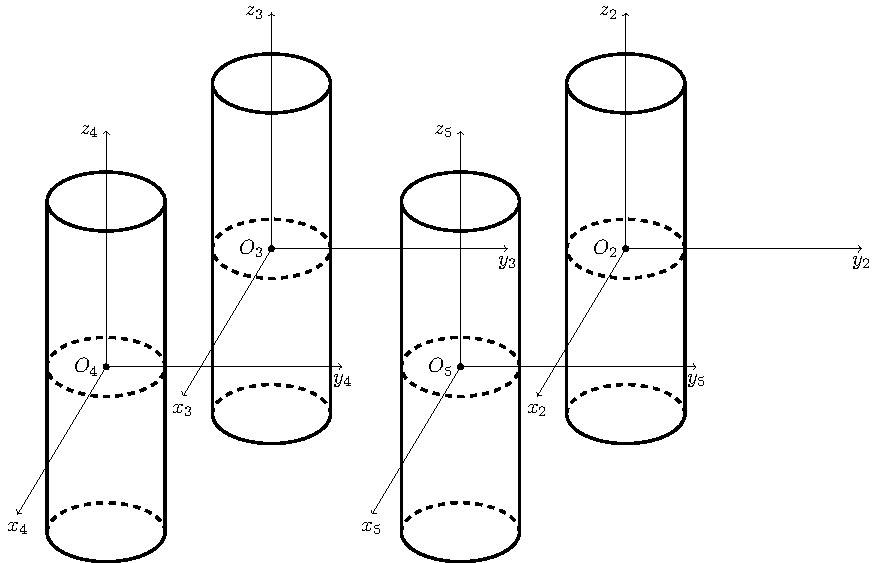
\includegraphics[width=12cm]{cylinders-4.pdf}
\caption{Схематическое представление задачи}
\label{fig:cyl-4a}
\end{figure}

Считаем, что цилиндрические полости свободны от нагрузки. Для определения НДС в рассматриваемом теле необходимо решить краевую задачу для уравнения Ламе

\begin{equation}
\Delta {\bf{U}} + \frac{1}{{1 - 2\sigma }}\nabla div{\bf{U}} = 0
\label{eq:7:27}
\end{equation}

\noindent с граничными условиями

\begin{equation}
{\bf{FU}}{|_{{\Gamma _j}}} = 0
\label{eq:7:18}
\end{equation}

\noindent и кусочно-постоянными напряжениями на цилиндрическом образце

\begin{equation}
{\left. {{\bf{FU}}} \right|_{{\Gamma _0}}} = \left\{ \begin{array}{l}
T,\;\;\;{\mkern 1mu} {\kern 1pt} |z| \le h/2\\
0,\;\;\;{\mkern 1mu} {\kern 1pt} |z| > h/2
\end{array} \right\}{{\bf{e}}_\rho },
\label{eq:7:19}
\end{equation}

\noindent где $\mathbf{U}$~--- вектор перемещений; $\mathbf{FU}$~--- отвечающий $\mathbf{U}$ вектор усилий на соответствующей граничной поверхности; границы цилиндров $\Gamma_j$ задаются уравнениями $\rho_j=R_j$ ($j=\overline{1,N}$).

Решение задачи будем искать в виде

\begin{equation}
\mathbf{U}=\mathbf{U}^++\mathbf{U}^-,
\end{equation}

\noindent где

\begin{equation}
{\bf{U}}^+ = \sum\limits_{j = 1}^N {\sum\limits_{s = 1}^3 {\sum\limits_{m =  - \infty }^\infty  {\int\limits_{ - \infty }^\infty  {A_{s,m}^{(j)}} } } } (\lambda ){\bf{U}}_{s,\lambda ,m}^{ + (3)}\left( {{\rho _j},{z_j},{\varphi _j}} \right)d\lambda;
\end{equation}

\begin{equation}
{{\bf{U}}}^- = \sum\limits_{s = 1}^3 {\sum\limits_{m =  - \infty }^\infty  {\mathop \int \limits_{ - \infty }^\infty  } } A_{s,m}^{(0)}(\lambda ){\bf{U}}_{s,\lambda ,m}^{ - (3)}\left( {{\rho _1},{z_1},{\varphi _1}} \right)d\lambda;
\end{equation}

\noindent $A_{s,m}^{(j)}(\lambda )$~--- неизвестные функции;

\begin{equation}
\mathbf{U}_{s,\lambda,m}^{\pm(3)}(\rho,\varphi,z)=\lambda^{-1}\mathbf{D}_s u_{\lambda,m}^{\pm(3)}(\rho,\varphi,z);\quad s=1,3;
\label{eq:7:1}
\end{equation}

\begin{equation}
\mathbf{U}_{2,\lambda,m}^{\pm(3)}(\rho,\varphi,z)=\lambda^{-1}\mathbf{B}_2 u_{\lambda,m}^{\pm(3)}(\rho,\varphi,z),
\label{eq:7:2}
\end{equation}

\begin{equation}
\mathbf{B}_2=\left(x\frac{\partial}{\partial x}+y\frac{\partial}{\partial y}\right)\nabla-\chi\Big[\mathbf{e}_z\times[\nabla\times\mathbf{e}_z]\Big];
\end{equation}

\begin{equation*}
u_{\lambda,m}^{+(3)}(\rho,\varphi,z)=e^{i\lambda z+im\varphi}\tilde K_m(\lambda\rho),\quad
u_{\lambda,m}^{-(3)}(\rho,\varphi,z)=e^{i\lambda z+im\varphi}I_m(\lambda\rho),
\end{equation*}

\noindent где $\mathbf{D}_1=\nabla$, $\mathbf{D}_2=z\nabla-\chi\mathbf{e}_z$, $\mathbf{D}_3=i[\nabla\times\mathbf{e}_z]$ (здесь $i$~--- мнимая единица); $I_m(x)$~--- модифицированная функция Бесселя, $\tilde K_m(x)=(\mathrm{sign}\,x)^m K_m(|x|)$, $K_m(x)$~--- функция Макдональда; $\chi=3-4\sigma$, $u_{\lambda,m}^{\pm(3)}$~--- полный набор частных решений уравнения Лапласа в цилиндрических координатах.

В развернутой координатной форме базисные решения~\eqref{eq:7:1}, \eqref{eq:7:2} имеют вид:

\begin{equation}
\mathbf{U}_{1,\lambda,m}^{\pm(3)}(\rho,\varphi,z)=\mp u_{\lambda,m-1}^{\pm(3)}\mathbf{e}_{-1}\mp u_{\lambda,m+1}^{\pm(3)}\mathbf{e}_1+iu_{\lambda,m}^{\pm(3)}\mathbf{e}_0;
\label{eq:7:4}
\end{equation}

\begin{equation}
\mathbf{U}_{2,\lambda,m}^{\pm(3)}(\rho,\varphi,z)=\mp(D-\chi)\left[u_{\lambda,m-1}^{\pm(3)}\mathbf{e}_{-1}+
u_{\lambda,m+1}^{\pm(3)}\mathbf{e}_1\right]+iDu_{\lambda,m}^{\pm(3)}\mathbf{e}_0;
\label{eq:7:5}
\end{equation}

\begin{equation}
\mathbf{U}_{3,\lambda,m}^{\pm(3)}(\rho,\varphi,z)=\pm u_{\lambda,m-1}^{\pm(3)}\mathbf{e}_{-1}\mp u_{\lambda,m+1}^{\pm(3)}\mathbf{e}_1,
\label{eq:7:6}
\end{equation}

\noindent где $D=\rho\dfrac{\partial}{\partial\rho}$; $\mathbf{e}_{-1}=\dfrac{1}{2}(\mathbf{e}_\rho+i\mathbf{e}_\varphi)e^{i\varphi}$; $\mathbf{e}_1=\dfrac{1}{2}(\mathbf{e}_\rho-i\mathbf{e}_\varphi)e^{-i\varphi}$; $\mathbf{e}_0=\mathbf{e}_z$; $(\mathbf{e}_\rho,\mathbf{e}_\varphi,\mathbf{e}_z)$~--- орты цилиндрической системы координат.

Вектор напряжений на площадке с нормалью $\mathbf{n}$

\begin{equation}
\mathbf{FU}=2G\left[\frac{\sigma}{1-2\sigma}\mathbf{n}\,\mathrm{div}\mathbf{U}+\frac{\partial\mathbf{U}}{\partial\mathbf{n}}+\frac{1}{2}(\mathbf{n}\times\mathrm{rot}\mathbf{U})\right],
\label{eq:7:3}
\end{equation}

\noindent где $G$~--- модуль сдвига.

Применив к формулам~\eqref{eq:7:4}~--- \eqref{eq:7:6} оператор~\eqref{eq:7:3} на площадке с нормалью $\mathbf{n}=\mathbf{e}_\rho$, получим

\begin{equation}
\mathbf{FU}_{1,\lambda,m}^{\pm(3)}=\frac{2G}{\rho}\left\{\mp Du_{\lambda,m-1}^{\pm(3)}\mathbf{e}_{-1}\mp Du_{\lambda,m+1}^{\pm(3)}\mathbf{e}_1+iDu_{\lambda,m}^{\pm(3)}\mathbf{e}_0\right\};
\end{equation}
\begin{multline}
\mathbf{FU}_{2,\lambda,m}^{\pm(3)}=\frac{2G}{\rho}\left\{\mp\Big[(m-1)(m-1+2\sigma)+\lambda^2\rho^2+(2\sigma-3)D\Big]u_{\lambda,m-1}^{\pm(3)}\mathbf{e}_{-1}\mp\right.\\
\mp[(m+1)(m+1-2\sigma)+\lambda^2\rho^2+(2\sigma-3)D]u_{\lambda,m+1}^{\pm(3)}\mathbf{e}_1+\left.i[m^2+\lambda^2\rho^2(2\sigma-2)D]u_{\lambda,m}^{\pm(3)}\mathbf{e}_0\right\};
\end{multline}
\begin{equation}
\mathbf{FU}_{3,\lambda,m}^{\pm(3)}=\frac{G}{\rho}\left\{\pm(D+m-1)u_{\lambda,m-1}^{\pm(3)}\mathbf{e}_{-1}\mp\right.\left.(D-m-1)u_{\lambda,m+1}^{\pm(3)}\mathbf{e}_1-imu_{\lambda,m}^{\pm(3)}\mathbf{e}_0\right\}.
\end{equation}

Для удовлетворения граничных условий нам понадобятся теоремы сложения базисных решений уравнения Ламе для цилиндра:

\begin{equation}
{\bf{U}}_{s,\lambda ,m}^{ + (3)}\left( {{\rho _j},{z_j},{\varphi _j}} \right) = \sum\limits_{l =  - \infty }^\infty  {{{( - 1)}^l}} f_{\lambda ,m,j,\alpha }^{ + (33)l}{\bf{U}}_{s,\lambda ,l}^{ - (3)}\left( {{\rho _\alpha },{z_\alpha },{\varphi _\alpha }} \right);
\label{eq:7:7}
\end{equation}

\begin{multline}
{\bf{U}}_{2,\lambda ,m}^{ + (3)}\left( {{\rho _j},{z_j},{\varphi _j}} \right) = \sum\limits_{l =  - \infty }^\infty  {{{( - 1)}^l}} \left[ {f_{\lambda ,m,j,\alpha }^{ + (33)l}{\bf{U}}_{2,\lambda ,l}^{ - (3)}\left( {{\rho _\alpha },{z_\alpha },{\varphi _\alpha }} \right) + } \right.\\
\left. { + \tilde f_{\lambda ,m,j,\alpha }^{ + (33)l}{\bf{U}}_{1,\lambda ,l}^{ - (3)}\left( {{\rho _\alpha },{z_\alpha },{\varphi _\alpha }} \right)} \right];
\label{eq:7:8}
\end{multline}

$$
f_{\lambda ,m,j,\alpha }^{ + (33)l} = u_{\lambda ,m - l}^{ + (3)}\left( {{\rho _{j\alpha }},{z_{j\alpha }},{\varphi _{j\alpha }}} \right),\quad
\tilde f_{\lambda ,m,j,\alpha }^{ + (33)l} = {\rho _{j\alpha }}\frac{\partial }{{\partial {\rho _{j\alpha }}}}u_{\lambda ,m - l}^{ + (3)}\left( {{\rho _{j\alpha }},{z_{j\alpha }},{\varphi _{j\alpha }}} \right);
$$

\begin{equation}
{\bf{U}}_{s,\lambda ,m}^{ - (3)}\left( {{\rho _0},{z_0},{\varphi _0}} \right) = \sum\limits_{l =  - \infty }^\infty  {f_{\lambda ,m,j}^{ - (33)l}{\bf{U}}_{s,\lambda ,l}^{ - (3)}\left( {{\rho _j},{z_j},{\varphi _j}} \right)};
\label{eq:7:9}
\end{equation}
\begin{equation}
{\bf{U}}_{2,\lambda ,m}^{ - (3)}\left( {{\rho _0},{z_0},{\varphi _0}} \right) = \sum\limits_{l =  - \infty }^\infty  {\left[ {f_{\lambda ,m,j}^{ - (33)l}{\bf{U}}_{2,\lambda ,l}^{ - (3)}\left( {{\rho _j},{z_j},{\varphi _j}} \right) + } \right.} \left. {\tilde f_{\lambda ,m,j}^{ - (33)l}{\bf{U}}_{1,\lambda ,l}^{ - (3)}\left( {{\rho _j},{z_j},{\varphi _j}} \right)} \right];
\label{eq:7:10}
\end{equation}
$$
f_{\lambda ,m,j}^{ - (33)l} = u_{\lambda ,m - l}^{ - (3)}\left( {{\rho _{0j}},{z_{0j}},{\varphi _{0j}}} \right),\quad
\tilde f_{\lambda ,m,j}^{ - (33)l} = {\rho _{0j}}\frac{\partial }{{\partial {\rho _{0j}}}}u_{\lambda ,m - l}^{ - (3)}\left( {{\rho _{0j}},{z_{0j}},{\varphi _{0j}}} \right);
$$

\begin{equation}
{\bf{U}}_{s,\lambda ,m}^{ + (3)}\left( {{\rho _j},{z_j},{\varphi _j}} \right) = \sum\limits_{l =  - \infty }^\infty  {f_{\lambda ,m,j}^{ - (33)l}{\bf{U}}_{s,\lambda ,l}^{ + (3)}\left( {{\rho _0},{z_0},{\varphi _0}} \right)};
\label{eq:7:11}
\end{equation}

\begin{multline}
{\bf{U}}_{2,\lambda ,m}^{ + (3)}\left( {{\rho _j},{z_j},{\varphi _j}} \right) = \sum\limits_{l =  - \infty }^\infty  {\left[ {f_{\lambda ,m,j}^{ - (33)l}{\bf{U}}_{2,\lambda ,l}^{ - (3)}\left( {{\rho _0},{z_0},{\varphi _0}} \right) + } \right.} \\
\left. { + \tilde f_{\lambda ,m,j}^{ - (33)l}{\bf{U}}_{1,\lambda ,l}^{ + (3)}\left( {{\rho _0},{z_0},{\varphi _0}} \right)} \right];
\label{eq:7:12}
\end{multline}
$$
f_{\lambda ,m,j}^{ - (33)l} = u_{\lambda ,m - l}^{ - (3)}\left( {{\rho _{0j}},{z_{0j}},{\varphi _{0j}}} \right),\quad
\tilde f_{\lambda ,m,j}^{ - (33)l} = {\rho _{0j}}\frac{\partial }{{\partial {\rho _{0j}}}}u_{\lambda ,m - l}^{ - (3)}\left( {{\rho _{0j}},{z_{0j}},{\varphi _{0j}}} \right).
$$

Запишем общее решение в системе координат с началами $O_0$ и $O_\alpha$ с помощью теорем сложения~\eqref{eq:7:7}~--- \eqref{eq:7:12}. В случае, если ячейка не является объемно центрированной,

\begin{multline}
{\bf{U}} = \sum\limits_{s = 1}^3 {\sum\limits_{m =  - \infty }^\infty  {\int\limits_{ - \infty }^\infty\bigg\{  } } A_{s,m}^{(0)}(\lambda ){\bf{U}}_{s,\lambda ,m}^{ - (3)}({\rho _0},{z_0},{\varphi _0}) + \\
+ {\bf{U}}_{s,\lambda ,m}^{ + (3)}({\rho _0},{z_0},{\varphi _0})\sum\limits_{\alpha  = 1}^N {\sum\limits_{t = 1}^3 {\sum\limits_{l =  - \infty }^\infty  {A_{t,l}^{(\alpha )}} } } (\lambda )\bigg[{\delta _{st}} + {\delta _{s1}}{\delta _{t2}}{\rho _{0\alpha }}\frac{\partial }{{\partial {\rho _{0\alpha }}}}\bigg]u_{\lambda ,l - m}^{ - (3)}({\rho _{0\alpha }},0,{\varphi _{0\alpha }})\bigg\} d\lambda;
\label{eq:7:13}
\end{multline}

\begin{multline}
{\bf{U}} = \sum\limits_{s = 1}^3 {\sum\limits_{m =  - \infty }^\infty  {\int\limits_{ - \infty }^\infty  \bigg\{  } } A_{s,m}^{(\alpha )}(\lambda ){\bf{U}}_{s,\lambda ,m}^{ + (3)}({\rho _\alpha },{z_\alpha },{\varphi _\alpha }) + \\
+ {\bf{U}}_{s,\lambda ,m}^{ - (3)}({\rho _\alpha },{z_\alpha },{\varphi _\alpha })\sum\limits_{t = 1}^3 {\sum\limits_{l =  - \infty }^\infty  {A_{t,l}^{(0)}} } (\lambda )\bigg[{\delta _{st}} + {\delta _{s1}}{\delta _{t2}}{\rho _{0\alpha }}\frac{\partial }{{\partial {\rho _{0\alpha }}}}\bigg]u_{\lambda ,l - m}^{ - (3)}({\rho _{0\alpha }},0,{\varphi _{0\alpha }}) + \\
+ \sum\limits_{j \ne \alpha } {{\bf{U}}_{s,\lambda ,m}^{ - (3)}} ({\rho _\alpha },{z_\alpha },{\varphi _\alpha })\sum\limits_{t = 1}^3 {\sum\limits_{l =  - \infty }^\infty  {A_{t,l}^{(j)}} } (\lambda ){( - 1)^m}\bigg[{\delta _{st}} + \\
+ {\delta _{s1}}{\delta _{t2}}{\rho _{j\alpha }}\frac{\partial }{{\partial {\rho _{j\alpha }}}}\bigg]u_{\lambda ,l - m}^{ + (3)}({\rho _{j\alpha }},0,{\varphi _{j\alpha }})\bigg\} d\lambda.
\label{eq:7:14}
\end{multline}

В случае объемно центрированной ячейки вектор перемещения имеет вид:

\begin{multline}
{\bf{U}} = \sum\limits_{s = 1}^3 {\sum\limits_{m =  - \infty }^\infty  {\int\limits_{ - \infty }^\infty  \bigg\{  } } A_{s,m}^{(0)}(\lambda ){\bf{U}}_{s,\lambda ,m}^{ - (3)}({\rho _1},{z_1},{\varphi _1}) + A_{s,m}^{(1)}(\lambda ){\bf{U}}_{s,\lambda ,m}^{ + (3)}({\rho _1},{z_1},{\varphi _1}) + \\
+ {\bf{U}}_{s,\lambda ,m}^{ + (3)}({\rho _1},{z_1},{\varphi _1})\sum\limits_{\alpha  = 2}^N {\sum\limits_{t = 1}^3 {\sum\limits_{l =  - \infty }^\infty  {A_{t,l}^{(\alpha )}} } } (\lambda )\bigg[{\delta _{st}} + \\
+ {\delta _{s1}}{\delta _{t2}}{\rho _{1\alpha }}\frac{\partial }{{\partial {\rho _{1\alpha }}}}\bigg]u_{\lambda ,l - m}^{ - (3)}({\rho _{1\alpha }},0,{\varphi _{1\alpha }})\bigg\} d\lambda;
\label{eq:7:15}
\end{multline}

\begin{multline}
{\bf{U}} = \sum\limits_{s = 1}^3 {\sum\limits_{m =  - \infty }^\infty  {\int\limits_{ - \infty }^\infty  \bigg\{  } } A_{s,m}^{(0)}(\lambda ){\bf{U}}_{s,\lambda ,m}^{ - (3)}({\rho _1},{z_1},{\varphi _1}) + A_{s,m}^{(1)}(\lambda ){\bf{U}}_{s,\lambda ,m}^{ + (3)}({\rho _1},{z_1},{\varphi _1}) + \\
+ {\bf{U}}_{s,\lambda ,m}^{ - (3)}({\rho _1},{z_1},{\varphi _1})\sum\limits_{\alpha  = 2}^N {\sum\limits_{t = 1}^3 {\sum\limits_{l =  - \infty }^\infty  {A_{t,l}^{(\alpha )}} } } (\lambda ){( - 1)^l}\bigg[{\delta _{st}} + \\
+ {\delta _{s1}}{\delta _{t2}}{\rho _{1\alpha }}\frac{\partial }{{\partial {\rho _{1\alpha }}}}\bigg]u_{\lambda ,l - m}^{ + (3)}({\rho _{1\alpha }},0,{\varphi _{1\alpha }})\bigg\} d\lambda;
\label{eq:7:16}
\end{multline}

\begin{multline}
{\bf{U}} = \sum\limits_{s = 1}^3 {\sum\limits_{m =  - \infty }^\infty  {\int\limits_{ - \infty }^\infty  \bigg\{  } } A_{s,m}^{(\alpha )}(\lambda ){\bf{U}}_{s,\lambda ,m}^{ + (3)}({\rho _\alpha },{z_\alpha },{\varphi _\alpha }) + \\
+ {\bf{U}}_{s,\lambda ,m}^{ - (3)}({\rho _\alpha },{z_\alpha },{\varphi _\alpha })\sum\limits_{t = 1}^3 {\sum\limits_{l =  - \infty }^\infty  {A_{t,l}^{(0)}} } (\lambda )\bigg[{\delta _{st}} + {\delta _{s1}}{\delta _{t2}}{\rho _{0\alpha }}\frac{\partial }{{\partial {\rho _{0\alpha }}}}\bigg]u_{\lambda ,l - m}^{ - (3)}({\rho _{0\alpha }},0,{\varphi _{0\alpha }}) + \\
+ \sum\limits_{j \ne \alpha } {{\bf{U}}_{s,\lambda ,m}^{ - (3)}} ({\rho _\alpha },{z_\alpha },{\varphi _\alpha })\sum\limits_{t = 1}^3 {\sum\limits_{l =  - \infty }^\infty  {A_{t,l}^{(j)}} } (\lambda ){( - 1)^m}\bigg[{\delta _{st}} + \\
+ {\delta _{s1}}{\delta _{t2}}{\rho _{j\alpha }}\frac{\partial }{{\partial {\rho _{j\alpha }}}}\bigg]u_{\lambda ,l - m}^{ + (3)}({\rho _{j\alpha }},0,{\varphi _{j\alpha }})\bigg\} d\lambda ,\qquad {\kern 1pt} \alpha  \ne 1.
\label{eq:7:17}
\end{multline}

Переходя в формулах~\eqref{eq:7:13}~--- \eqref{eq:7:17} к напряжениям на поверхности $\Gamma_j$, согласно соотношениям~\eqref{eq:7:18}, \eqref{eq:7:19}, относительно неизвестных функций $A_{s,m}^{(j)}(\lambda)$ получаем бесконечную систему линейных алгебраических уравнений\sloppy

\begin{multline}
\sum\limits_{s = 1}^3 \bigg\{  A_{s,m}^{(0)}(\lambda ){\bf{G}}_{s,\lambda ,m}^{ - (3)}({R_0},G,\sigma ) + {\bf{G}}_{s,\lambda ,m}^{ + (3)}({R_0},G,\sigma ) \times \\
\times \sum\limits_{\alpha  = 1}^N {\sum\limits_{t = 1}^3 {\sum\limits_{l =  - \infty }^\infty  {A_{t,l}^{(\alpha )}} } } (\lambda )\bigg[{\delta _{st}} + {\delta _{s1}}{\delta _{t2}}{\rho _{0\alpha }}\frac{\partial }{{\partial {\rho _{0\alpha }}}}\bigg]u_{\lambda ,l - m}^{ - (3)}({\rho _{0\alpha }},0,{\varphi _{0\alpha }})\bigg\}  = \\
= \frac{T}{\pi }\frac{{\sin \lambda h}}{\lambda }{\delta _{m0}}(1,1,0),
\label{eq:7:20}
\end{multline}

\begin{multline}
\sum\limits_{s = 1}^3 \bigg\{  A_{s,m}^{(\alpha )}(\lambda ){\bf{G}}_{s,\lambda ,m}^{ + (3)}(R,G,\sigma ) + {\bf{G}}_{s,\lambda ,m}^{ - (3)}(R,G,\sigma ) \times \\
\times \sum\limits_{t = 1}^3 {\sum\limits_{l =  - \infty }^\infty  {A_{t,l}^{(0)}} } (\lambda )\bigg[{\delta _{st}} + {\delta _{s1}}{\delta _{t2}}{\rho _{0\alpha }}\frac{\partial }{{\partial {\rho _{0\alpha }}}}\bigg]u_{\lambda ,l - m}^{ - (3)}({\rho _{0\alpha }},0,{\varphi _{0\alpha }}) + \\
+ \sum\limits_{j \ne \alpha } {{\bf{G}}_{s,\lambda ,m}^{ - (3)}} (R,G,\sigma )\sum\limits_{t = 1}^3 {\sum\limits_{l =  - \infty }^\infty  {A_{t,l}^{(j)}} } (\lambda ){( - 1)^m}\bigg[{\delta _{st}} + {\delta _{s1}}{\delta _{t2}}{\rho _{j\alpha }}\frac{\partial }{{\partial {\rho _{j\alpha }}}}\bigg] \times \\
\times u_{\lambda ,l - m}^{ + (3)}({\rho _{j\alpha }},0,{\varphi _{j\alpha }})\bigg\}  = 0.
\label{eq:7:21}
\end{multline}

Система записана в случае отсутствия объемного центрирования. Для объем\-но-цент\-ри\-ро\-ван\-ной ячейки разрешающая система имеет вид:

\begin{multline}
\sum\limits_{s = 1}^3 \bigg\{  A_{s,m}^{(0)}(\lambda ){\bf{G}}_{s,\lambda ,m}^{ - (3)}({R_0},G,\sigma ) + A_{s,m}^{(1)}(\lambda ){\bf{G}}_{s,\lambda ,m}^{ + (3)}({R_0},G,\sigma ) + \\
+ {\bf{G}}_{s,\lambda ,m}^{ + (3)}({R_0},G,\sigma )\sum\limits_{\alpha  = 2}^N {\sum\limits_{t = 1}^3 {\sum\limits_{l =  - \infty }^\infty  {A_{t,l}^{(\alpha )}} } } (\lambda )\bigg[{\delta _{st}} + \\
+ {\delta _{s1}}{\delta _{t2}}{\rho _{0\alpha }}\frac{\partial }{{\partial {\rho _{0\alpha }}}}\bigg]u_{\lambda ,l - m}^{ - (3)}({\rho _{0\alpha }},0,{\varphi _{0\alpha }})\bigg\}  = \frac{T}{\pi }\frac{{\sin \lambda h}}{\lambda }{\delta _{m0}}(1,1,0);
\label{eq:7:22}
\end{multline}

\begin{multline}
\sum\limits_{s = 1}^3 \bigg\{  A_{s,m}^{(\alpha )}(\lambda ){\bf{G}}_{s,\lambda ,m}^{ + (3)}(R,G,\sigma ) + {\bf{G}}_{s,\lambda ,m}^{ - (3)}(R,G,\sigma ) \times \\
\times \sum\limits_{t = 1}^3 {\sum\limits_{l =  - \infty }^\infty  {A_{t,l}^{(0)}} } (\lambda )\bigg[{\delta _{st}} + {\delta _{s1}}{\delta _{t2}}{\rho _{0\alpha }}\frac{\partial }{{\partial {\rho _{0\alpha }}}}\bigg]u_{\lambda ,l - m}^{ - (3)}({\rho _{0\alpha }},0,{\varphi _{0\alpha }}) + \\
+ \sum\limits_{j \ne \alpha } {{\bf{G}}_{s,\lambda ,m}^{ - (3)}} (R,G,\sigma )\sum\limits_{t = 1}^3 {\sum\limits_{l =  - \infty }^\infty  {A_{t,l}^{(j)}} } (\lambda ){( - 1)^m}\bigg[{\delta _{st}} + {\delta _{s1}}{\delta _{t2}}{\rho _{j\alpha }}\frac{\partial }{{\partial {\rho _{j\alpha }}}}\bigg] \times \\
\times u_{\lambda ,l - m}^{ + (3)}({\rho _{j\alpha }},0,{\varphi _{j\alpha }})\bigg\}  = 0,\qquad {\kern 1pt} \alpha  \ne 1;
\label{eq:7:23}
\end{multline}

\begin{multline}
\sum\limits_{s = 1}^3 \bigg\{  A_{s,m}^{(0)}(\lambda ){\bf{G}}_{s,\lambda ,m}^{ - (3)}(R,G,\sigma ) + A_{s,m}^{(1)}(\lambda ){\bf{G}}_{s,\lambda ,m}^{ + (3)}(R,G,\sigma ) + \\
+ \mathop \sum \limits_{j = 2}^N {\bf{G}}_{s,\lambda ,m}^{ - (3)}(R,G,\sigma )\sum\limits_{t = 1}^3 {\sum\limits_{l =  - \infty }^\infty  {A_{t,l}^{(j)}} } (\lambda ){( - 1)^m}\bigg[{\delta _{st}} + {\delta _{s1}}{\delta _{t2}}{\rho _{j1}}\frac{\partial }{{\partial {\rho _{j1}}}}\bigg] \times \\
\times u_{\lambda ,l - m}^{ + (3)}({\rho _{j1}},0,{\varphi _{j1}})\bigg\}  = 0;
\label{eq:7:24}
\end{multline}

\begin{equation}
G_{1,\lambda ,m}^{ \pm ( - 1)}(R) =  \mp \frac{{2G}}{R}D\tilde u_{\lambda ,m - 1}^{ \pm (3)}(R),\, G_{1,\lambda ,m}^{ \pm (1)}(R) =  \pm \frac{{2G}}{R}D\tilde u_{\lambda ,m + 1}^{ \pm (3)}(R);
\label{eq:7:35}
\end{equation}
\begin{equation}
G_{1,\lambda ,m}^{ \pm (0)}(R) = \frac{{2G}}{R}iD\tilde u_{\lambda ,m}^{ \pm (3)}(R);
\label{eq:7:36}
\end{equation}
\begin{equation}
G_{2,\lambda ,m}^{ \pm ( - 1)}(R) = \mp \frac{{2G}}{R}\bigg[(m - 1)(m - 1 + 2\sigma ) + {\lambda ^2}{R^2} + (2\sigma  - 3)D\bigg]\tilde u_{\lambda ,m - 1}^{ \pm (3)}(R);
\label{eq:7:37}
\end{equation}
\begin{equation}
G_{2,\lambda ,m}^{ \pm (1)}(R) = \mp \frac{{2G}}{R}\bigg[ (m + 1)(m + 1 - 2\sigma ) + {\lambda ^2}{R^2} + (2\sigma  - 3)D \bigg]\tilde u_{\lambda ,m + 1}^{ \pm (3)}(R);
\label{eq:7:38}
\end{equation}
\begin{equation}
G_{2,\lambda ,m}^{ \pm (0)}(R) = \frac{{2G}}{R}i\left[ {{m^2} + {\lambda ^2}{R^2} + (2\sigma  - 2)D} \right]\tilde u_{\lambda ,m}^{ \pm (3)}(R);
\label{eq:7:39}
\end{equation}
\begin{equation}
G_{3,\lambda ,m}^{ \pm ( - 1)}(R) =  \pm \frac{G}{R}\left( {D + m - 1} \right)\tilde u_{\lambda ,m - 1}^{ \pm (3)}(R);
\label{eq:7:40}
\end{equation}
\begin{equation}
G_{3,\lambda ,m}^{ \pm (1)}(R) =  \mp \frac{G}{R}\left( {D - m - 1} \right)\tilde u_{\lambda ,m + 1}^{ \pm (3)}(R);
\label{eq:7:41}
\end{equation}
\begin{equation}
G_{3,\lambda ,m}^{ \pm (0)}(R) =  - \frac{G}{R}im\tilde u_{\lambda ,m}^{ \pm (3)}(R);
\label{eq:7:41a}
\end{equation}
\begin{equation}
\tilde u_{\lambda ,m}^{ \pm (3)}(R) = \left\{ \begin{array}{l}
{{\tilde K}_m}\left( {\lambda R} \right)\\
{I_m}\left( {\lambda R} \right)
\end{array} \right\}.
\label{eq:7:42}
\end{equation}

\section{Анализ разрешающей системы}

\begin{theorem}
При любом $\lambda\neq 0$ оператор системы~\eqref{eq:7:20}, \eqref{eq:7:21} является фредгольмовым в гильбертовом пространстве $l_2$ при выполнении условий $R_j+R_\alpha<\rho_{j\alpha}$ ($j\neq\alpha$; $j,\alpha=1\div N$), $\rho_{0\alpha}+R_\alpha<R_0$ ($\alpha=1\div N$). 
\end{theorem}
\begin{proof}
Путем переобозначения неизвестных функций
\begin{equation}
A_{s,m}^{(j)}(\lambda)=\frac{\tilde A_{s,m}^{(j)}(\lambda)}{K_m(|\lambda|R_j)},\quad(j=1\div N),\quad A_{s,m}^{(0)}(\lambda)=\frac{\tilde A_{s,m}^{(0)}(\lambda)}{I_m(\lambda R_0)}
\end{equation}
и решения системы относительно $\tilde A_{s,m}^{(j)}(\lambda)$ можно представить систему~\eqref{eq:7:20}, \eqref{eq:7:21} в виде
\begin{equation}
\tilde A_{s,m}^{(\alpha)}(\lambda)+\sum\limits_{j\neq\alpha}\sum\limits_{p=1}^3\sum\limits_{l=-\infty}^\infty T_{1,\alpha,s,m}^{j,p,l}\tilde A_{p,l}^{(j)}(\lambda)+\sum\limits_{p=1}^3\sum\limits_{l=-\infty}^\infty T_{2,\alpha,s,m}^{p,l}\tilde A_{p,l}^{(0)}(\lambda)=0,
\label{eq:27}
\end{equation}
\begin{equation}
\tilde A_{s,m}^{(0)}(\lambda)+\sum\limits_{j=1}^N\sum\limits_{p=1}^3\sum\limits_{l=-\infty}^\infty T_{3,s,m}^{j,p,l}\tilde A_{p,l}^{(j)}(\lambda)=F_{s,m}(\lambda).
\label{eq:28}
\end{equation}
Опустим явную запись матричных коэффициентов. Заметим, что модули матричных коэффициентов $\left|T_{1,\alpha,s,m}^{j,p,l}\right|$, $\left|T_{2,\alpha,s,m}^{p,l}\right|$, $\left|T_{3,s,m}^{j,p,l}\right|$ оцениваются сверху конечными линейными комбинациями выражений вида~\eqref{eq:24}~--- \eqref{eq:26} соответственно:
\begin{equation}
\bigg|\frac{I_m(\lambda R_\alpha)}{K_l(|\lambda|R_j)}K_{m-l}(|\lambda|\rho_{j\alpha})\bigg|;
\label{eq:24}
\end{equation}
\begin{equation}
\bigg|\frac{I_m(\lambda R_\alpha)}{I_l(\lambda R_0)}I_{m-l}(|\lambda|\rho_{0\alpha})\bigg|;
\label{eq:25}
\end{equation}
\begin{equation}
\bigg|\frac{K_m(|\lambda|R_0)}{K_l(|\lambda|R_j)}I_{m-l}(\lambda\rho_{j0})\bigg|.
\label{eq:26}
\end{equation}
При этом были использованы оценки определителей разрешающих систем первой краевой задачи теории упругости для внутренности и внешности цилиндра, полученные в работе~\cite{Nikolaev1998}.

Для доказательства теоремы достаточно показать, выполнение следующих условий для матричных коэффициентов системы~\eqref{eq:27}, \eqref{eq:28}:
\begin{equation}
\sum\limits_{m=-\infty}^\infty\sum\limits_{l=-\infty}^\infty\bigg|T_{1,\alpha,s,m}^{j,p,l}\bigg|^2<\infty,
\end{equation}
\begin{equation}
\sum\limits_{m=-\infty}^\infty\sum\limits_{l=-\infty}^\infty\bigg|T_{2,\alpha,s,m}^{p,l}\bigg|^2<\infty,
\end{equation}
\begin{equation}
\sum\limits_{m=-\infty}^\infty\sum\limits_{l=-\infty}^\infty\bigg|T_{3,s,m}^{j,p,l}\bigg|^2<\infty.
\end{equation}
\par Рассмотрим теорему сложения гармонических функций~\cite{Nikolaev2011}:
\begin{equation}
u_{\lambda,m}^{+(3)}(\rho_j,\varphi_j,z_j)=\sum\limits_{l=-\infty}^\infty(-1)^l u_{\lambda,m-l}^{+(3)}(\rho_{j\alpha},\varphi_{j\alpha},z_{j\alpha}) u_{\lambda,l}^{-(3)}(\rho_\alpha,\varphi_\alpha,z_\alpha).
\end{equation}
Это разложение можно интепретировать как представление функции $u_{\lambda,m}^{+(3)}(\rho_j,\varphi_j,z_j)$ рядом Фурье по переменной $\varphi_\alpha\in[0,2\pi]$. Тогда для этого разложения справедливо равенство Парсеваля{\sloppy\par}
\begin{equation}
\sum\limits_{l=-\infty}^\infty\bigg|K_{m-l}(|\lambda|\rho_{j\alpha})\bigg|^2\bigg|I_l(\lambda\rho_\alpha)\bigg|^2=\frac{1}{2\pi}\int\limits_0^{2\pi}\bigg|K_m(|\lambda|\rho_j)\bigg|^2d\varphi_\alpha.
\label{eq:32}
\end{equation}
В силу оценок~\eqref{eq:24}~--- \eqref{eq:26} для доказательства теоремы достаточно показать сходимость рядов
\begin{equation}
\sum\limits_{m=-\infty}^\infty\sum\limits_{l=-\infty}^\infty\bigg|\frac{I_m(\lambda R_\alpha)}{K_l(|\lambda|R_j)}K_{m-l}(|\lambda|\rho_{j\alpha})\bigg|^2,
\label{eq:29}
\end{equation}
\begin{equation}
\sum\limits_{m=-\infty}^\infty\sum\limits_{l=-\infty}^\infty\bigg|\frac{I_m(\lambda R_\alpha)}{I_l(\lambda R_0)}I_{m-l}(|\lambda|\rho_{0\alpha})\bigg|^2,
\label{eq:30}
\end{equation}
\begin{equation}
\sum\limits_{m=-\infty}^\infty\sum\limits_{l=-\infty}^\infty\bigg|\frac{K_m(|\lambda|R_0)}{K_l(|\lambda|R_j)}I_{m-l}(\lambda\rho_{j0})\bigg|^2.
\label{eq:31}
\end{equation}
\par В работе~\cite{Nikolaev1998} доказана оценка
\begin{equation}
I_m(z)K_m(z)>\frac{c}{m^2+1}(1+2z)^{-1},\quad m\ge 0,\quad z>0,
\label{eq:37}
\end{equation}
где $c>0$~--- некоторая постоянная. Тогда ряд~\eqref{eq:29} можно мажорировать рядом
\begin{equation*}
\sum\limits_{m=-\infty}^\infty\sum\limits_{l=-\infty}^\infty\bigg|I_l(\lambda R_\alpha)I_m(\lambda R_j)K_{m-l}(|\lambda|\rho_{j\alpha})\bigg|^2.
\end{equation*}
Подставим в тождество~\eqref{eq:32} $\rho_\alpha=R_\alpha$, после чего домножим обе его части на $|I_m(\lambda R_j)|^2$ и просуммируем по $m$ от $-\infty$ до $\infty$. В результате получим
\begin{multline}
\sum\limits_{m=-\infty}^\infty\sum\limits_{l=-\infty}^\infty\bigg|I_l(\lambda R_\alpha)I_m(\lambda R_j)K_{m-l}(|\lambda|\rho_{j\alpha})\bigg|^2=\\
=\frac{1}{2\pi}\int\limits_0^{2\pi}\sum\limits_{m=0}^\infty\bigg|I_m(\lambda R_j)\bigg|^2\bigg|K_m(|\lambda|\rho_j)\bigg|_{|_{\rho_\alpha=R_\alpha}}^2d\varphi_\alpha.
\label{eq:33}
\end{multline}
Из асимптотических формул при $m\rightarrow\infty$~\cite{Lebedev}
\begin{equation}
I_m(z)=\bigg(\frac{z}{2}\bigg)^m\frac{1}{m!}\bigg[1+O(m^{-1})\bigg],
\label{eq:35}
\end{equation}
\begin{equation}
K_m(z)=\frac{2^{m-1}(m-1)!}{z^m}\bigg[1+O(m^{-1})\bigg]
\label{eq:36}
\end{equation}
следует, что ряд в левой части~\eqref{eq:33} сходится при условии $\rho_j>R_j$. Определим минимальное значение $\rho_j^{min}$ при произвольных значениях угла $\varphi_\alpha$. Из соотношений между цилиндрическими координатами в системах с началами $O_j$ и $O_\alpha$ следует, что при $\rho_\alpha=R_\alpha$
\begin{equation*}
\rho_j=\sqrt{\rho_{j\alpha}^2+R_\alpha^2+2\rho_{j\alpha}R_\alpha\cos{(\varphi_\alpha-\varphi_{j\alpha})}}
\end{equation*}
и минимальное значение $\rho_j$ достигается при условии $\varphi_\alpha-\varphi_{j\alpha}=\pi$ и равняется $\rho_j^{min}=\rho_{j\alpha}-R_\alpha$ ($\rho_{j\alpha}>R_\alpha$~--- естественное геометрическое условие в постановке задачи).

Таким образом, условие сходимости ряда будет удовлетворено, если $\rho_j^{min}>R_j$. Оно означает, что $R_j+R_\alpha<\rho_{j\alpha}$.{\sloppy\par}

Аналогично можно записать такое равенство:
\begin{multline}
\sum\limits_{m=-\infty}^\infty\sum\limits_{l=-\infty}^\infty\bigg|K_m(|\lambda| R_0)I_l(\lambda R_\alpha)I_{m-l}(\lambda\rho_{0\alpha})\bigg|^2=\\
=\frac{1}{2\pi}\int\limits_0^{2\pi}\sum\limits_{m=0}^\infty\bigg|K_m(|\lambda|R_0)\bigg|^2\bigg|I_m(\lambda\rho_0)\bigg|_{|_{\rho_\alpha=R_\alpha}}^2d\varphi_\alpha.
\label{eq:34}
\end{multline}
На основании асимптотик~\eqref{eq:35}, \eqref{eq:36} ряд в формуле~\eqref{eq:34} сходится при условии $\rho_0<R_0$. На поверхности $\rho_\alpha=R_\alpha$ справедливо $\rho_0^{max}=\rho_{0\alpha}+R_\alpha$. Поэтому условием сходимости ряда~\eqref{eq:34} является неравенство $\rho_0^{max}<R_0$ или $\rho_{0\alpha}+R_\alpha<R_0$.

В силу оценки~\eqref{eq:37} сходимость ряда~\eqref{eq:31} при условии $\rho_{0j}+R_j<R_0$ следует из сходимости ряда~\eqref{eq:34}.
\end{proof}


\section{Анализ напряженного состояния пористого материала}

Численное решение разрешающих систем~\eqref{eq:7:20}~--- \eqref{eq:7:24} позволяет найти распределение напряжений в пористом материале при любой структуре упаковки. Далее будут рассмотрены следующие варианты упаковки волокон: тетрагональная и гексагональная и их центрированные модификации.

Рассмотрим геометрическую конфигурацию, представленную на рис.~\ref{f:7:6}.

\begin{figure}[h!]
\centering
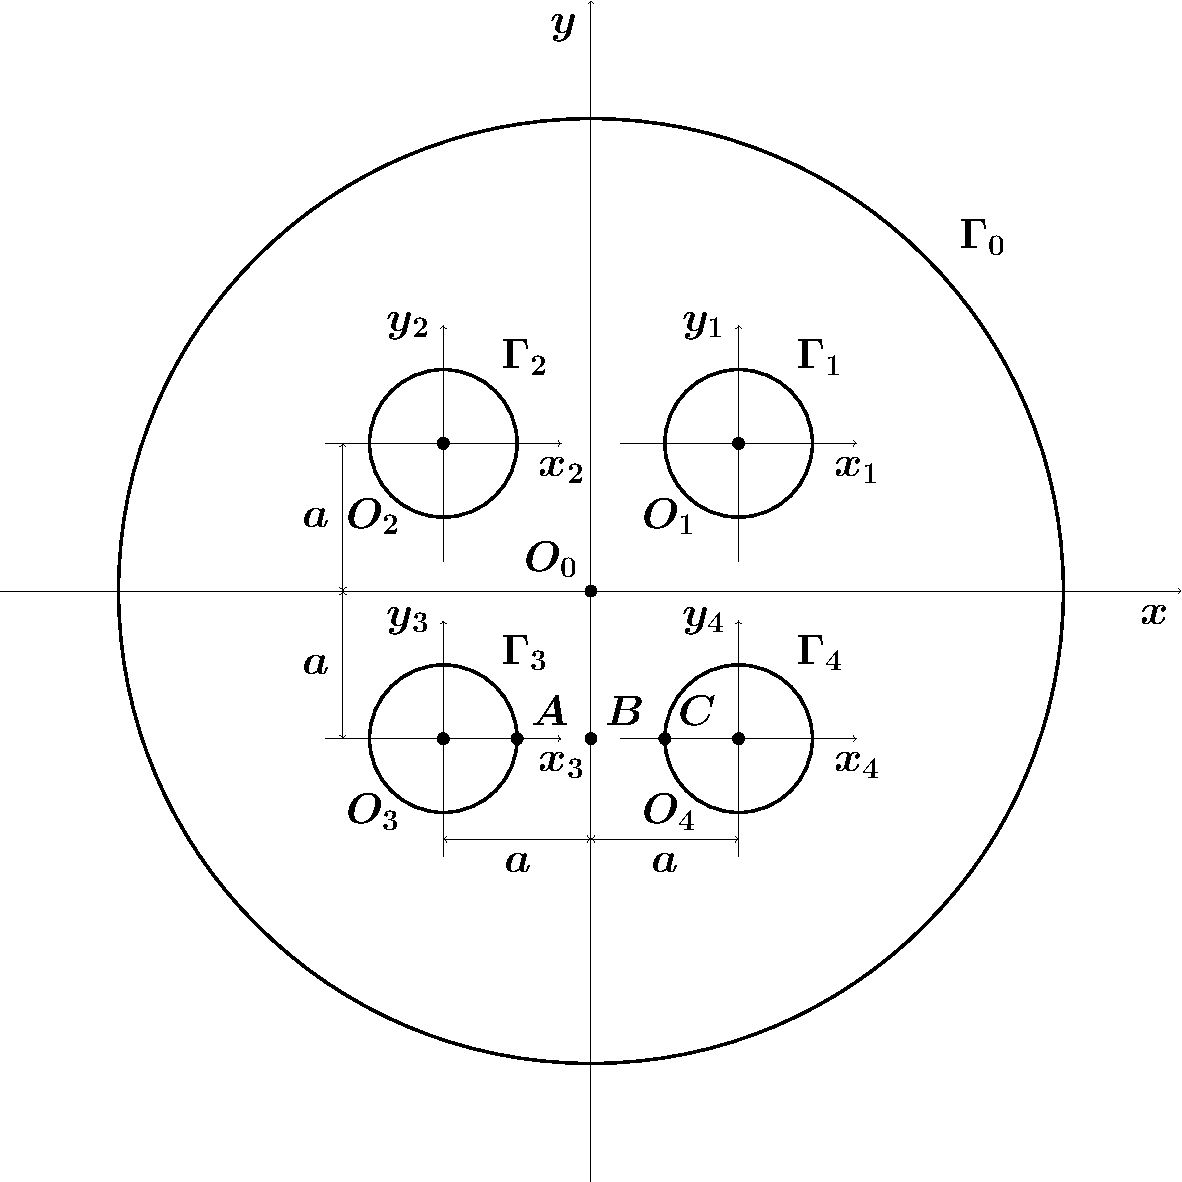
\includegraphics[width=8cm]{fig_7-6.pdf}
\caption{\centering Цилиндрический образец пористого материала с тетрагональной структурой упаковки}
\label{f:7:6}
\end{figure}

Коэффициент Пуассона материала $\sigma=0.38$, что соответствует материалу матрицы из эпоксидных смол. Толщина кольца, по которому прикладывается постоянная внешняя нагрузка $T$, $h=0.5R_0$; также считаем, что $R=1$, $R_0=10R$.

Несобственные интегралы, фигурирующие в формулах для определения напряжений, вычисляются по квадратурным формулам Гаусса~--- Лагерра с количеством узлов $n=20$.

Квадратурная формула Гаусса~--- Лагерра аппроксимирует значения интегралов вида

\begin{equation}
\int\limits_0^{ + \infty } {{e^{ - x}}} f(x)dx
\end{equation}

\noindent рядом по $n$ точкам

\begin{equation}
\int\limits_0^{ + \infty } {{e^{ - x}}} f(x)dx \approx \sum\limits_{i = 1}^n {{w_i}} f({x_i}),
\end{equation}

\noindent где $x_i$~--- это $i$-й корень полинома Лагерра $L_n(x)$, а коэффициенты

\begin{equation}
{w_i} = \frac{{{x_i}}}{{{{(n + 1)}^2}L_{n + 1}^2({x_i})}}.
\end{equation}

\begin{table}[h!]
\caption{Проверка граничных условий}
\centering
$
\begin{array}{|c|c|c|c|c|}
\hline
\varphi & 0 & \dfrac{\pi}{2} & \pi & \dfrac{3\pi}{2} \\
\hline
\sigma_\rho & -5.2303\times 10^{-7} & -5.22332\times 10^{-7} & 1.65745\times 10^{-7} & 1.65171\times 10^{-7} \\
\hline
\end{array}
$
\label{t:7:1}
\end{table}

Результаты вычислений, приведенные в табл.~\ref{t:7:1}, свидетельствуют о том, что граничные условия на поверхности полостей выполняются с высокой точностью. Численный анализ показывает, что точность выполнения граничных условий можно повышать, увеличивая количество удерживаемых слагаемых $m_{max}$ в бесконечных суммах по методу редукции.

\begin{table}[h!]
\caption{Сходимость метода редукции}
\centering
$
\begin{array}{|c|c|c|c|c|}
\hline
m_{max} & 3 & 5 & 10 & 20 \\
\hline
\sigma_x & 0.278206 & 0.283708 & 0.283728 & 0.283728 \\
\hline
\sigma_y & 0.694919 & 0.693852 & 0.693843 & 0.693843 \\
\hline
\sigma_z & -0.220889 & -0.219252 & -0.219248 & -0.219248 \\
\hline
\end{array}
$
\label{t:7:2}
\end{table}

Сходимость метода редукции проверена в средней точке на оси, соединяющей центры 4-й и 5-й полостей. Из данных, приведенных в табл.~\ref{t:7:2}, можно сделать вывод, что метод редукции для данной системы сходится достаточно быстро. Для получения по крайней мере четырех верных значащих цифр в величине напряжений достаточно удерживать 11 слагаемых в бесконечных суммах, тогда как 21 слагаемое дает все шесть верных значащих цифр.

\begin{table}[h!]
\caption{Сравнение локальных и глобальных моделей}
\centering
$
\begin{array}{|c|c|c|c|c|}
\hline
\text{Кол-во полостей} & 1 & 2 & 4 & 16 \\
\hline
\sigma_x & 0.35721 & 0.293982 & 0.283728 & 0.414127 \\
\hline
\sigma_y & 0.601521 & 0.728503 & 0.693843 & 0.56664 \\
\hline
\sigma_z & -0.212649 & -0.202628 & -0.219248 & -0.227097 \\
\hline
\end{array}
$
\label{t:7:3}
\end{table}

Сравнение локальных и глобальных моделей проводится численно путем сравнения величин напряжений в одной точке образца для различного количества полостей, окружающих эту точку. Из анализа данных, приведенных в табл.~\ref{t:7:3}, можно сделать вывод, что напряженное состояние ($\sigma_z$) в направлении, поперечном плоскости действия нагрузки (вдоль оси образца), практически не зависит от количества рассматриваемых полостей в модели. Добавление учета внешнего слоя полостей приводит к незначительному перераспределению напряжений $\sigma_x$ и $\sigma_y$. Таким образом, можно сделать вывод, что в целом напряженное состояние в пористом материале для данной геометрической конфигурации можно моделировать локально, учитывая только самых ближних ``соседей''.

%\subsection{Одиночная полость в цилиндрическом образце}
%
%\sidefig(75mm){
%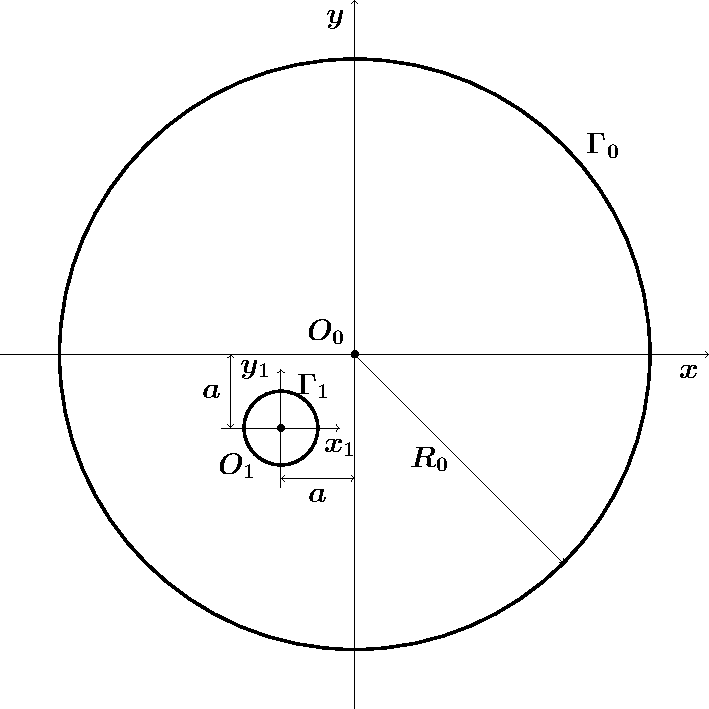
\includegraphics[width=7.5cm]{cav1.pdf}
%\caption{\centering Одиночная полость в цилиндрическом образце}
%\label{f:7:7}
%}{На рис.~\ref{f:7:8} представлены графики распределения напряжений $\sigma_\rho/T$ на диаметре цилиндрического образца, проходящего через центр полости вне ее границы в плоскостях $z=0$, $z=h/2$ и $z=h$ при фиксированных параметрах $\sigma=0.38$, $R_0=10R$, $h/R_0=0.5$; линиям 1, 2, 3 соответствуют графики напряжений в плоскостях $z=0$, $z=h/2$ и $z=h$ на большей части диаметра, а линиям 4, 5, 6~--- на меньшей части. Отрезок $[0,1]$ на оси $Ox$ на графике задает относительное расстояние между точками, соединяющими граничные поверхности внешнего цилиндра и полости на рис.~\ref{f:7:7}. Из анализа графиков, приведенных на рис.~\ref{f:7:8}, можно сделать вывод,} что выполняются граничные условия на цилиндрической полости, свободной от нагрузок по условию задачи, и на внешней границе цилиндра, где приложена кусочно-постоянная нормальная нагрузка.
%
%\begin{figure}
%\centering\footnotesize
%\parbox[b]{7.5cm}{\centering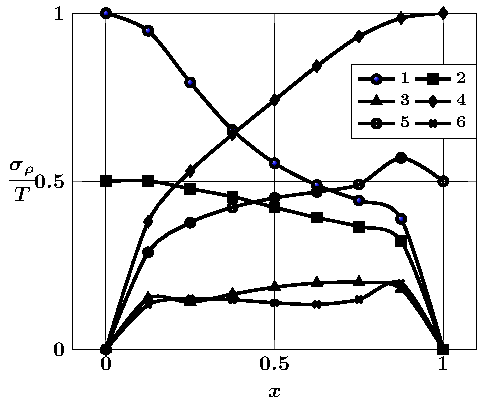
\includegraphics[width=7.5cm]{image-1.pdf}
%\caption{Напряжения $\sigma_\rho/T$ для конфигурации, представленной на~рис.~\ref{f:7:7}
%\label{f:7:8}}}\hfil\hfil
%\parbox[b]{7.5cm}{\centering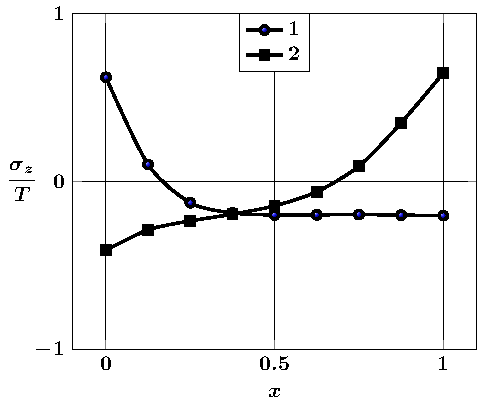
\includegraphics[width=7.5cm]{image-1-z.pdf}
%\caption{Напряжения $\sigma_z/T$ для конфигурации, представленной на~рис.~\ref{f:7:7}
%\label{f:7:9}}}
%\end{figure}
%
%На рис.~\ref{f:7:8} представлены графики распределения напряжений $\sigma_\rho/T$ на диаметре цилиндрического образца, проходящего через центр полости вне ее границы в плоскостях $z=0$, $z=h/2$ и $z=h$ при фиксированных параметрах $\sigma=0.38$, $R_0=10R$, $h/R_0=0.5$; линиям 1, 2, 3 соответствуют графики напряжений в плоскостях $z=0$, $z=h/2$ и $z=h$ на большей части диаметра, а линиям 4, 5, 6~--- на меньшей части. Отрезок $[0,1]$ на оси $Ox$ на графике задает относительное расстояние между точками, соединяющими граничные поверхности внешнего цилиндра и полости на рис.~\ref{f:7:7}. Из анализа графиков, приведенных на рис.~\ref{f:7:8}, можно сделать вывод, что выполняются граничные условия на цилиндрической полости, свободной от нагрузок по условию задачи, и на внешней границе цилиндра, где приложена кусочно-постоянная нормальная нагрузка.
%
%На рис.~\ref{f:7:9} представлены графики распределения напряжений $\sigma_z/T$ на диаметре цилиндрического образца, проходящего через центр полости вне ее границы в плоскости $z=0$ при фиксированных параметрах $\sigma=0.38$, $R_0=10R$, $h/R_0=0.5$; линия 1 соответствует графику на большей части диаметра, линия 2~--- на меньшей части.
%
%\subsection{Две полости в цилиндрическом образце}
%
%На рис.~\ref{f:7:83}, \ref{f:7:85}, \ref{f:7:87}, \ref{f:7:89}, \ref{f:7:91}, \ref{f:7:93}, \ref{f:7:11}, \ref{f:7:12} представлены нормальные компоненты тензора напряжений в декартовых координатах на оси, соединяющей пару цилиндрических полостей (рис.~\ref{f:7:10a}). Фиксированными являются параметры $\sigma=0.38$, $R_0=10R$, $a/R=2.0$, полости сдвинуты относительно центра цилиндрического образца на величину $a$ вдоль осей $x$ и $y$. Изменяется параметр приложенной к образцу нормальной внешней нагрузки $h/R_0=0.5$ и $h/R_0=1.0$.
%
%Из анализа графиков, представленных на рис.~\ref{f:7:11}, можно сделать вывод, что выполняются граничные условия на цилиндрических полостях.
%
%Максимальные по модулю напряжения наблюдаются в средней точке отрезка для напряжений $\sigma_x/T$ и $\sigma_z/T$ и на концах отрезка, т.~е. на границе цилиндров, для напряжений $\sigma_y/T$. Таким образом, основная концентрация напряжений наблюдается на границах полостей, на площадках, к ним перпендикулярных. Следует отметить, что увеличение интенсивности приложенной внешней нагрузки в два раза не приводит к аналогичному увеличению нормальных напряжений: напряжения $\sigma_y/T$ увеличиваются в среднем примерно в полтора раза, напряжения $\sigma_x/T$ по максимальной величине~--- менее чем в два раза, напряжения $\sigma_z/T$ практически не меняются при этом. 
%
%Таким образом, определяющими для напряженного состояния данного образца при данных нагрузках являются напряжения $\sigma_y/T$, максимальные величины которых почти в два раза превышают интенсивность приложенной внешней нагрузки.
%
%Косвенным элементом верификации полученных результатов может служить симметричный характер кривых при симметричных граничных условиях задачи.
%
%\begin{figure}
%\centering\footnotesize
%\parbox[b]{7.5cm}{\centering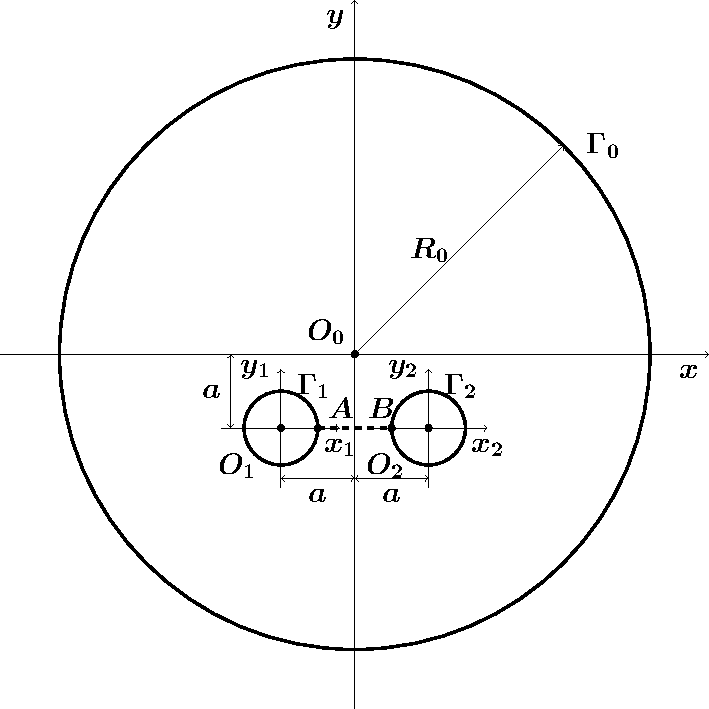
\includegraphics[width=7.5cm]{cav2a.pdf}
%\caption{Две полости в цилиндрическом образце, симметричные относительно оси $O_0y$ (конфигурация I)
%\label{f:7:10a}}}\hfil\hfil
%\parbox[b]{7.5cm}{\centering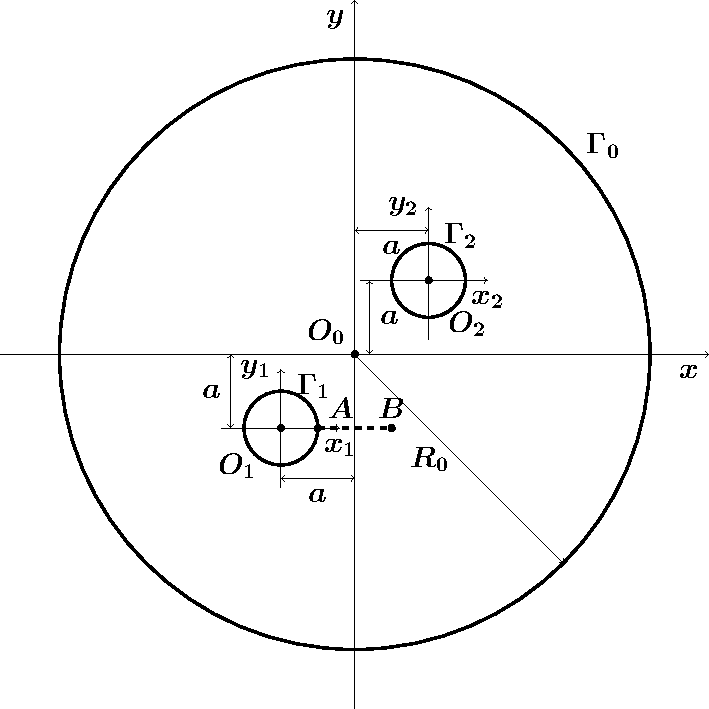
\includegraphics[width=7.5cm]{cav2b.pdf}
%\caption{Две центрально симметричные полости в цилиндрическом образце (конфигурация II)
%\label{f:7:10b}}}
%\end{figure}
%
%\begin{figure}
%\centering\footnotesize
%\parbox[b]{7.5cm}{\centering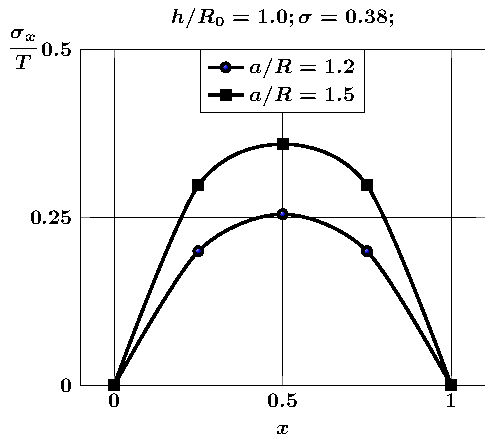
\includegraphics[width=7.5cm]{cav2-a-h10-r10-z0-sig_x.pdf}
%\caption{Распределение напряжений $\sigma_x/T$ на линии $AB$ в зависимости от относительного расстояния между полостями в плоскости $z=0$ в конфигурации I
%\label{f:7:83}}}\hfil\hfil
%\parbox[b]{7.5cm}{\centering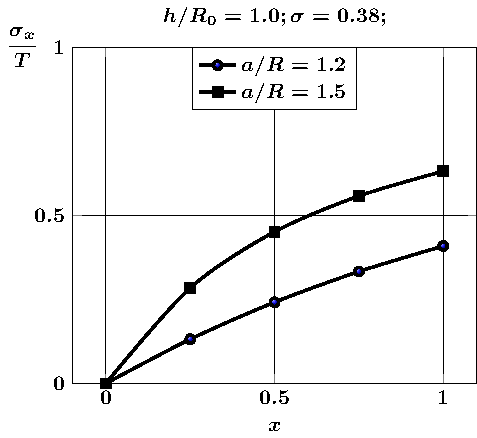
\includegraphics[width=7.5cm]{cav2a-a-h10-r10-z0-sig_x.pdf}
%\caption{Распределение напряжений $\sigma_x/T$ на линии $AB$ в зависимости от относительного расстояния между полостями в плоскости $z=0$ в конфигурации II
%\label{f:7:84}}}
%\end{figure}
%
%\begin{figure}
%\centering\footnotesize
%\parbox[b]{7.5cm}{\centering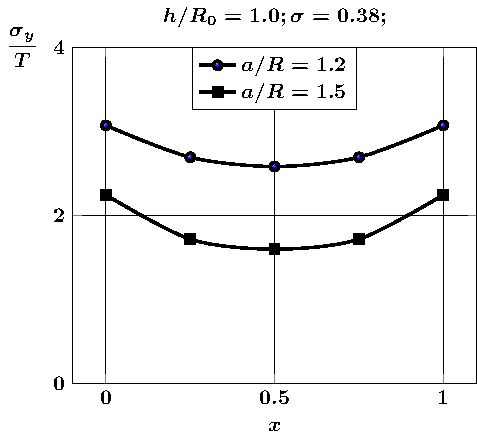
\includegraphics[width=7.5cm]{cav2-a-h10-r10-z0-sig_y.pdf}
%\caption{Распределение напряжений $\sigma_y/T$ на линии $AB$ в зависимости от относительного расстояния между полостями в плоскости $z=0$ в конфигурации I
%\label{f:7:85}}}\hfil\hfil
%\parbox[b]{7.5cm}{\centering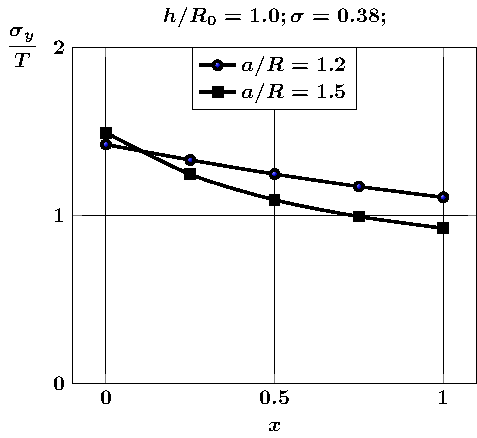
\includegraphics[width=7.5cm]{cav2a-a-h10-r10-z0-sig_y.pdf}
%\caption{Распределение напряжений $\sigma_y/T$ на линии $AB$ в зависимости от относительного расстояния между полостями в плоскости $z=0$ в конфигурации II
%\label{f:7:86}}}
%\end{figure}
%
%\begin{figure}
%\centering\footnotesize
%\parbox[b]{7.5cm}{\centering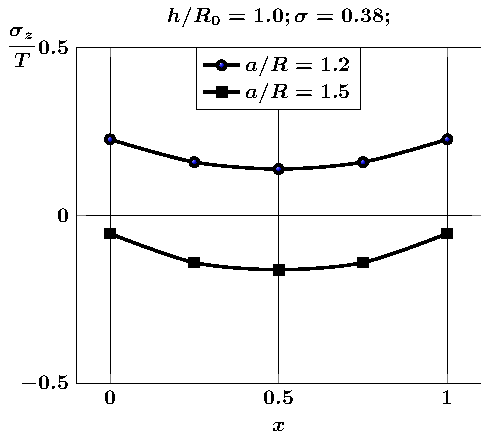
\includegraphics[width=7.5cm]{cav2-a-h10-r10-z0-sig_z.pdf}
%\caption{Распределение напряжений $\sigma_z/T$ на линии $AB$ в зависимости от относительного расстояния между полостями в плоскости $z=0$ в конфигурации I
%\label{f:7:87}}}\hfil\hfil
%\parbox[b]{7.5cm}{\centering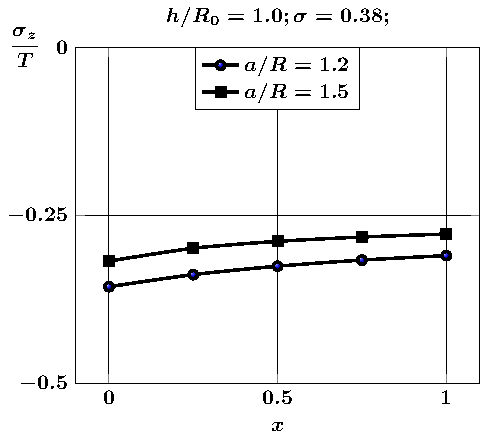
\includegraphics[width=7.5cm]{cav2a-a-h10-r10-z0-sig_z.pdf}
%\caption{Распределение напряжений $\sigma_z/T$ на линии $AB$ в зависимости от относительного расстояния между полостями в плоскости $z=0$ в конфигурации II
%\label{f:7:88}}}
%\end{figure}
%
%\begin{figure}
%\centering\footnotesize
%\parbox[b]{7.5cm}{\centering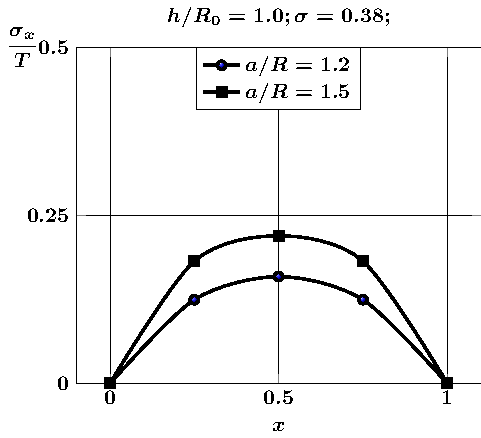
\includegraphics[width=7.5cm]{cav2-a-h10-r10-z1-sig_x.pdf}
%\caption{Распределение напряжений $\sigma_x/T$ на линии $AB$ в зависимости от относительного расстояния между полостями в плоскости $z=h/2$ в конфигурации I
%\label{f:7:89}}}\hfil\hfil
%\parbox[b]{7.5cm}{\centering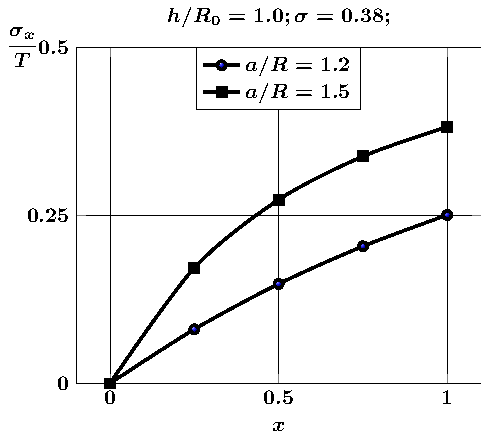
\includegraphics[width=7.5cm]{cav2a-a-h10-r10-z1-sig_x.pdf}
%\caption{Распределение напряжений $\sigma_x/T$ на линии $AB$ в зависимости от относительного расстояния между полостями в плоскости $z=h/2$ в конфигурации II
%\label{f:7:90}}}
%\end{figure}
%
%\begin{figure}
%\centering\footnotesize
%\parbox[b]{7.5cm}{\centering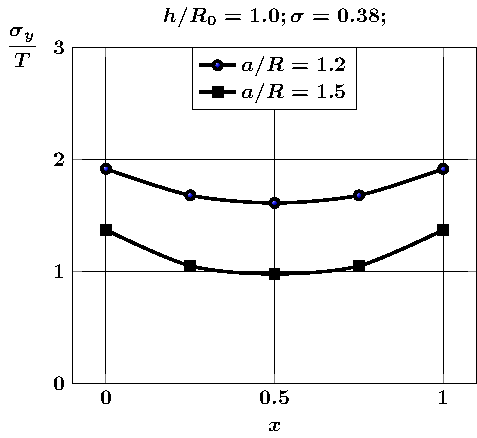
\includegraphics[width=7.5cm]{cav2-a-h10-r10-z1-sig_y.pdf}
%\caption{Распределение напряжений $\sigma_y/T$ на линии $AB$ в зависимости от относительного расстояния между полостями в плоскости $z=h/2$ в конфигурации I
%\label{f:7:91}}}\hfil\hfil
%\parbox[b]{7.5cm}{\centering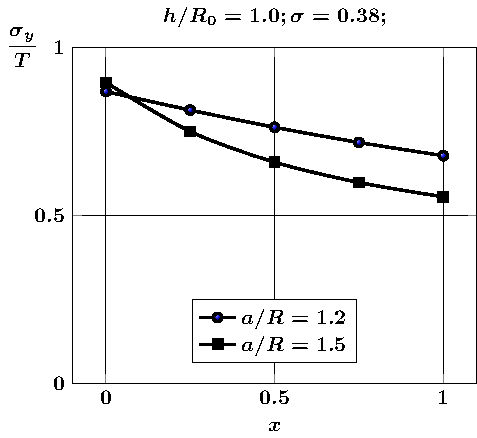
\includegraphics[width=7.5cm]{cav2a-a-h10-r10-z1-sig_y.pdf}
%\caption{Распределение напряжений $\sigma_y/T$ на линии $AB$ в зависимости от относительного расстояния между полостями в плоскости $z=h/2$ в конфигурации II
%\label{f:7:92}}}
%\end{figure}
%
%\begin{figure}
%\centering\footnotesize
%\parbox[b]{7.5cm}{\centering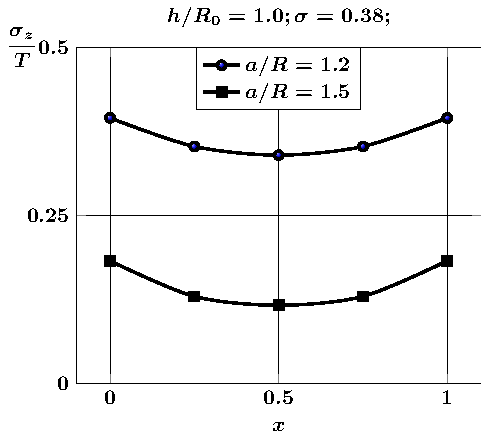
\includegraphics[width=7.5cm]{cav2-a-h10-r10-z1-sig_z.pdf}
%\caption{Распределение напряжений $\sigma_z/T$ на линии $AB$ в зависимости от относительного расстояния между полостями в плоскости $z=h/2$ в конфигурации I
%\label{f:7:93}}}\hfil\hfil
%\parbox[b]{7.5cm}{\centering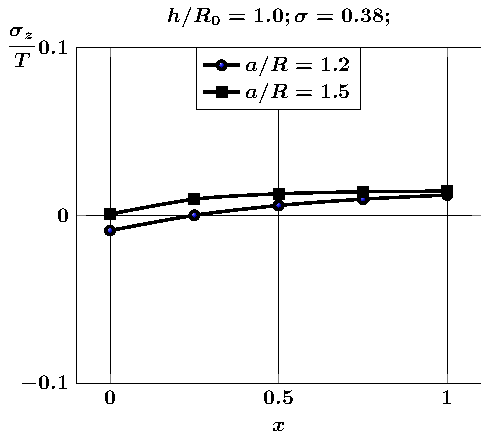
\includegraphics[width=7.5cm]{cav2a-a-h10-r10-z1-sig_z.pdf}
%\caption{Распределение напряжений $\sigma_z/T$ на линии $AB$ в зависимости от относительного расстояния между полостями в плоскости $z=h/2$ в конфигурации II
%\label{f:7:94}}}
%\end{figure}
%
%\begin{figure}
%\centering\footnotesize
%\parbox[b]{7.5cm}{\centering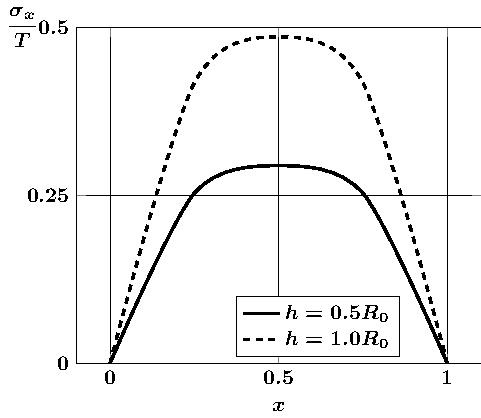
\includegraphics[width=7.5cm]{image-2-x.pdf}
%\caption{Напряжения $\sigma_x/T$ на линии $AB$ в зависимости от $h/R_0$ для конфигурации I
%\label{f:7:11}}}\hfil\hfil
%\parbox[b]{7.5cm}{\centering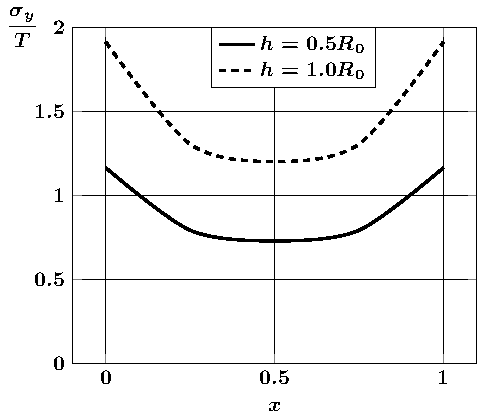
\includegraphics[width=7.5cm]{image-2-y.pdf}
%\caption{Напряжения $\sigma_y/T$ на линии $AB$ в зависимости от $h/R_0$ для конфигурации I
%\label{f:7:12}}}
%\end{figure}
%
%%\begin{figure}
%%\centering
%%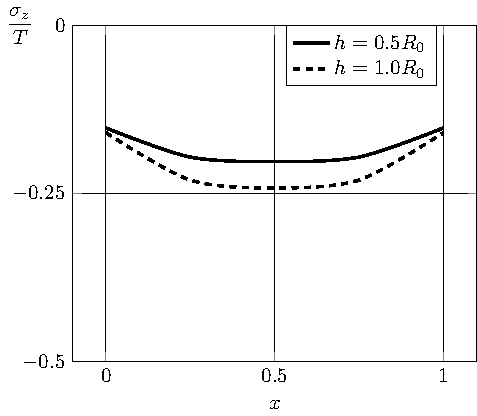
\includegraphics[width=12cm]{image-2-z.pdf}
%%\caption{Относительные напряжения $\sigma_z/T$ для конфигурации, представленной на рис.~\ref{f:7:10} в зависимости от изменения параметра $h/R_0$}
%%\label{f:7:13}
%%\end{figure}

\subsection{Тетрагональная структура расположения полостей в~цилиндрическом образце}

Рассмотрим цилиндрический образец пористого материала с тетрагональной структурой расположения полостей, как представлено на рис.~\ref{f:7:6}. Вычисления проведены при фиксированных параметрах $\sigma=0.38$, $h/R_0=1.0$, $R_0=10R$ в плоскости $z=0$. Каждая из полостей сдвинута относительно центра цилиндрического образца вдоль осей $x$ и $y$ на величину $a$. Относительное расстояние между цилиндрическими полостями изменялось следующим образом: $a/R=2.0$, $a/R=1.5$ и $a/R=1.2$, что соответствует пористости материала $\zeta=0.1964$, $\zeta=0.3491$ и $\zeta=0.5454$.

%На рис.~\ref{f:7:15} приведены относительные напряжения $\sigma_x/T$ на линии, соединяющей центры соседних полостей для конфигурации, представленной на рис.~\ref{f:7:6} в зависимости от изменения относительного расстояния между полостями. Из графиков, приведенных на рис.~\ref{f:7:15}, видно, что граничные условия на полостях выполняются для всех значений параметра $a/R$, а также падает концентрация напряжений $\sigma_x/T$ в средней точке отрезка при приближении полостей друг к другу.

%\begin{figure}[h!]
%\centering\footnotesize
%\parbox[b]{7.5cm}{\centering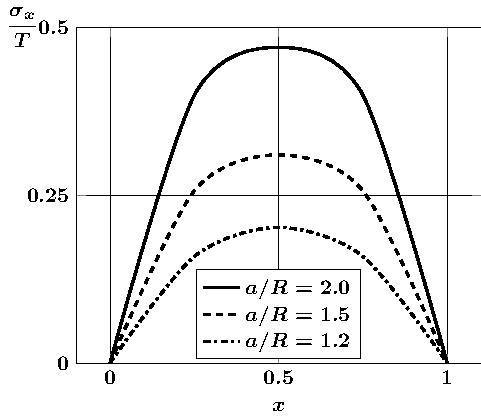
\includegraphics[width=7.5cm]{cav4_sig-x.pdf}
%\caption{Напряжения $\sigma_x/T$ на линии $AB$ для конфигурации, представленной на рис.~\ref{f:7:6}, в зависимости от относительного расстояния между полостями
%\label{f:7:15}}}\hfil\hfil
%\parbox[b]{7.5cm}{\centering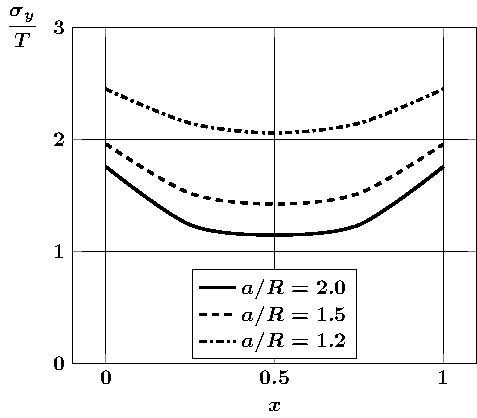
\includegraphics[width=7.5cm]{cav4_sig-y.pdf}
%\caption{Напряжения $\sigma_y/T$ на линии $AB$ для конфигурации, представленной на рис.~\ref{f:7:6}, в зависимости от относительного расстояния между полостями
%\label{f:7:16}}}
%\end{figure}

%На рис.~\ref{f:7:16} приведены относительные напряжения $\sigma_y/T$ на линии, соединяющей центры соседних полостей для конфигурации, представленной на рис.~\ref{f:7:6}, в зависимости от изменения относительного расстояния между полостями. Из графиков, приведенных на рис.~\ref{f:7:16}, видно, что растет концентрация напряжений $\sigma_y/T$ у смежных полюсов цилиндров при приближении полостей друг к другу. Следует также обратить внимание, что при достаточно высокой пористости материала (более 50~\%) максимальные по величине относительные напряжения $\sigma_y/T$ могут в 2.5 раза превосходить интенсивность внешних нагрузок, приложенных к образцу.
%
%На рис.~\ref{f:7:17} приведены относительные напряжения $\sigma_z/T$ на линии, соединяющей центры соседних полостей для конфигурации, представленной на рис.~\ref{f:7:6}, в зависимости от изменения относительного расстояния между полостями. Из графиков, приведенных на рис.~\ref{f:7:17}, видно, что напряжения $\sigma_z/T$ в несколько раз уменьшаются по абсолютной величине при приближении полостей друг к другу. При этом характер кривых сохраняется. Характерным также является то, что относительные напряжения $\sigma_z/T<0$ на всем рассматриваемом отрезке, то есть цилиндрический образец пористого материала в данном случае сжимается в продольном направлении.

%\sidefig(75mm){
%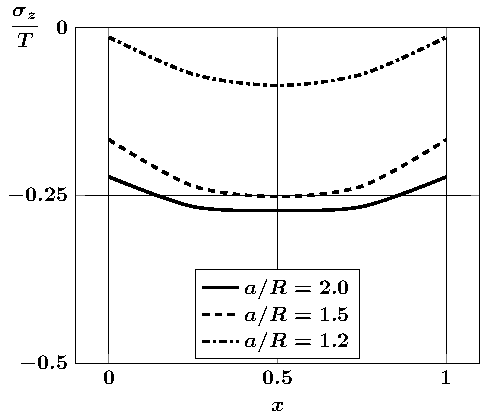
\includegraphics[width=7.5cm]{cav4_sig-z.pdf}
%\caption{Напряжения $\sigma_y/T$ на линии $AB$ для конфигурации, представленной на рис.~\ref{f:7:6}, в зависимости от относительного расстояния между полостями}
%\label{f:7:17}
%}

В табл.~\ref{t:7:4} приведены данные проверки граничных условий на одной из полостей в тетрагональной структуре при $R_0=10R$, $h/R_0=1.0$, $a/R=1.2$ и $m_{max}=20$, то есть в бесконечных суммах удерживаем 41 слагаемое. Из анализа приведенных данных видно, что граничные условия на полостях при близком их расположении в тетрагональной структуре выполняются достаточно хорошо.

На рис.~\ref{f:7:27} представлена тетрагональная структура расположения полостей в цилиндрическом образце с шестнадцатью полостями.

\begin{table}[h!]
\caption{Проверка граничных условий}
\centering
$
\begin{array}{|c|c|c|c|c|}
\hline
\varphi & 0 & \dfrac{\pi}{2} & \pi & \dfrac{3\pi}{2} \\
\hline
\sigma_\rho & -4.42278\times10^{-6} & -4.4263\times10^{-6} & 2.43255\times 10^{-6} & 2.42862\times 10^{-6} \\
\hline
\end{array}
$
\label{t:7:4}
\end{table}

На рис.~\ref{f:7:28}~--- \ref{f:7:30} представлены графики напряжений $\sigma_x/T$, $\sigma_y/T$ и $\sigma_z/T$ на линии, соединяющей центры соседних полостей для конфигурации, представленной на рис.~\ref{f:7:27}, в зависимости от изменения относительного расстояния между полостями в плоскостях $z=0$ и $z=h$. Из анализа данных графиков можно сделать вывод, что при приближении полостей концентрация напряжений $\sigma_y/T$ растет, а напряжения $\sigma_x/T$ уменьшаются как в плоскости $z=0$, так и в плоскости $z=h$. При переходе от плоскости $z=0$ к плоскости $z=h$ величины нормальных напряжений $\sigma_x/T$ и $\sigma_y/T$ уменьшаются, а напряжения $\sigma_z/T$ меняют знаки с отрицательных на положительные.

В табл.~\ref{t:7:5} приведены данные о сходимости метода редукции для случая шестнадцати полостей в тетрагональной структуре при $a/R=1.5$ и $h/R_0=1.0$ в средней точке отрезка $AB$. Данные таблицы говорят о том, что удовлетворительную точность можно получить уже при $m_{max}=5$.

\sidefig(75mm){
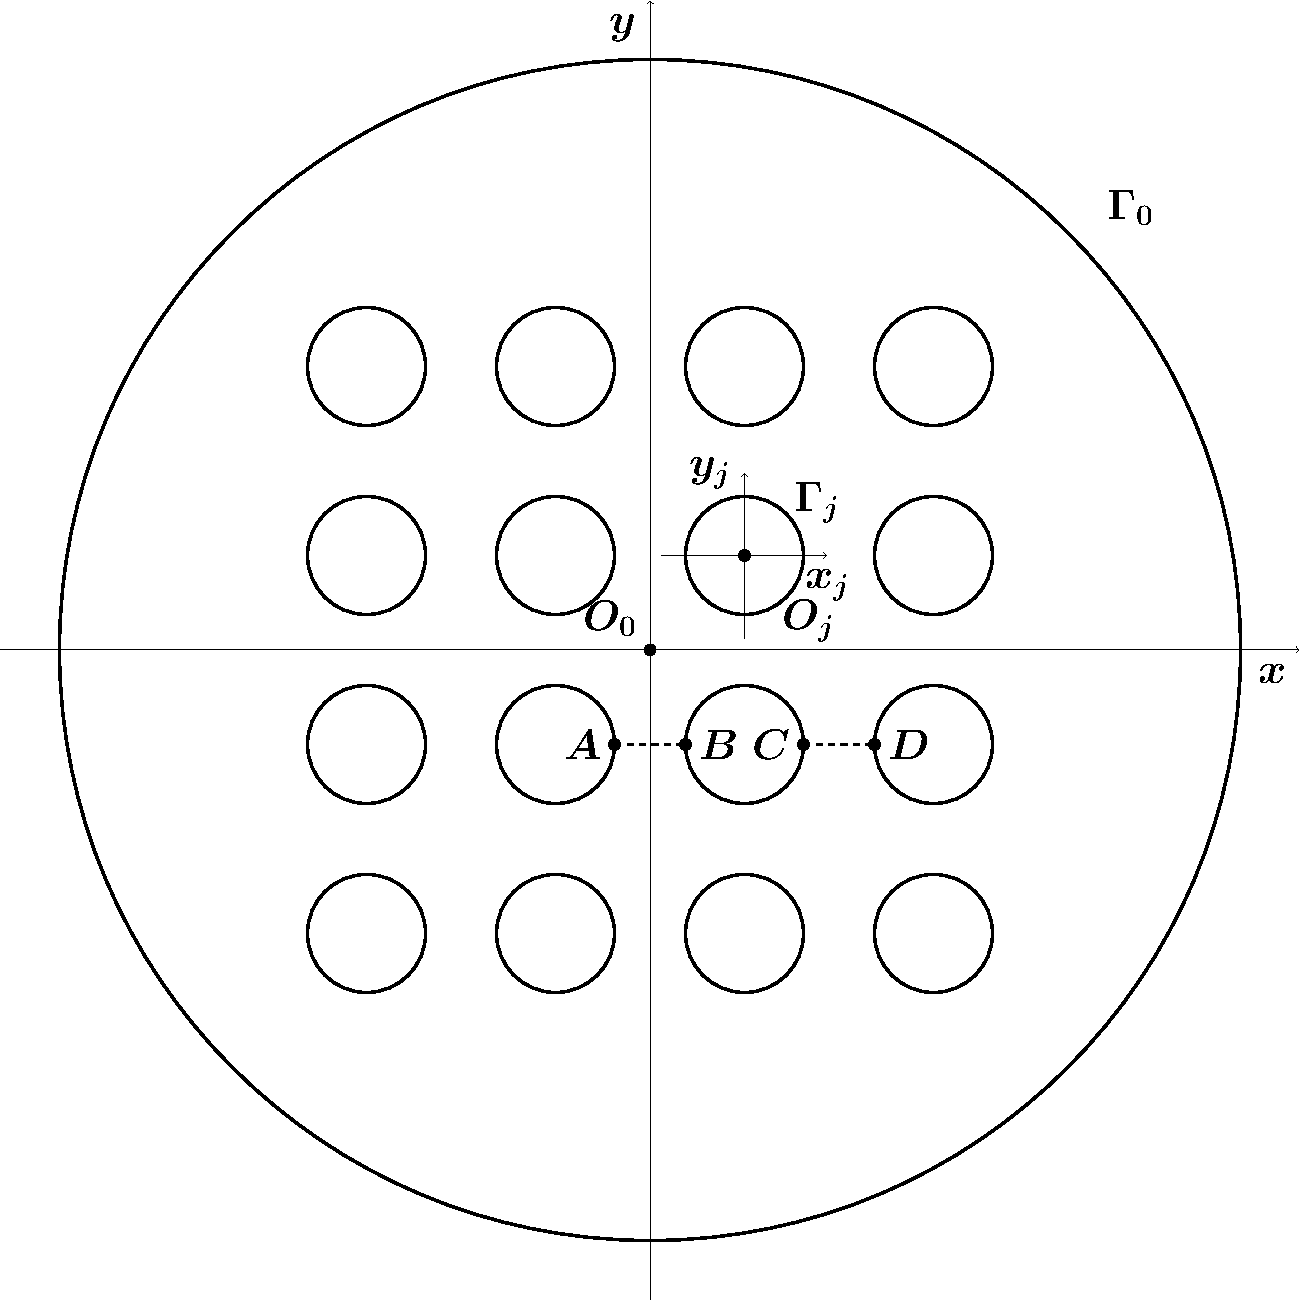
\includegraphics[width=7.5cm]{tetragonal-16.pdf}
\caption{Тетрагональная структура расположения полостей в цилиндрическом образце с шестнадцатью полостями}
\label{f:7:27}
}{На рис.~\ref{f:7:31} приведен график относительного напряжения $\sigma_y/T$ на линии, соединяющей центры соседних полостей, для конфигурации, представленной на рис.~\ref{f:7:27}, в зависимости от изменения интенсивности приложенной внешней нагрузки $h/R_0$ в плоскостях $z=0$ и $z=h$. График распределения напряжений $\sigma_y/T$ показывает, что области концентрации напряжений находятся вблизи границ полостей. При увеличении ширины кольца приложения внешней нормальной нагрузки в два раза напряжения $\sigma_y/T$ на линии $AB$ в плоскости $z=0$ увеличиваются более чем в полтора раза.\par\sloppy
}

\begin{figure}[h!]
\centering\footnotesize
\parbox[b]{7.5cm}{\centering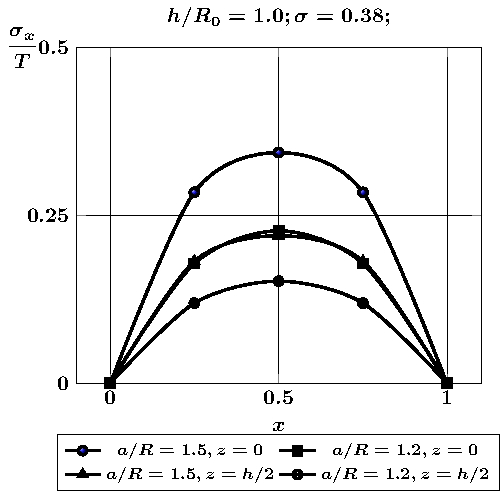
\includegraphics[width=7.5cm]{cav16-sig_x.pdf}
\caption{Напряжения $\sigma_x/T$ на линии $AB$ для конфигурации, представленной на рис.~\ref{f:7:27}, в зависимости от относительного расстояния между полостями в плоскостях $z=0$ и $z=h/2$
\label{f:7:28}}}\hfil\hfil
\parbox[b]{7.5cm}{\centering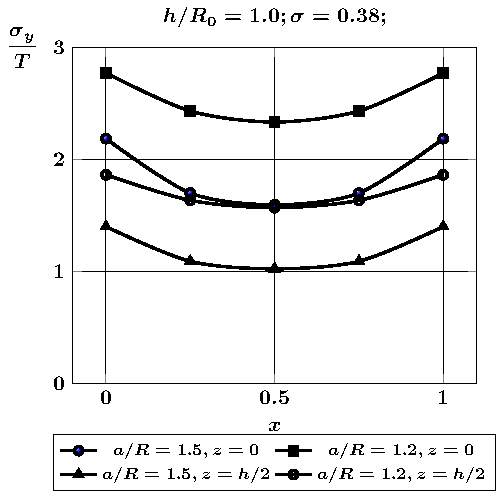
\includegraphics[width=7.5cm]{cav16-sig_y.pdf}
\caption{Напряжения $\sigma_y/T$ на линии $AB$ для конфигурации, представленной на рис.~\ref{f:7:27}, в зависимости от относительного расстояния между полостями в плоскостях $z=0$ и $z=h/2$
\label{f:7:29}}}
\end{figure}

\begin{figure}[h!]
\centering\footnotesize
\parbox[b]{7.5cm}{\centering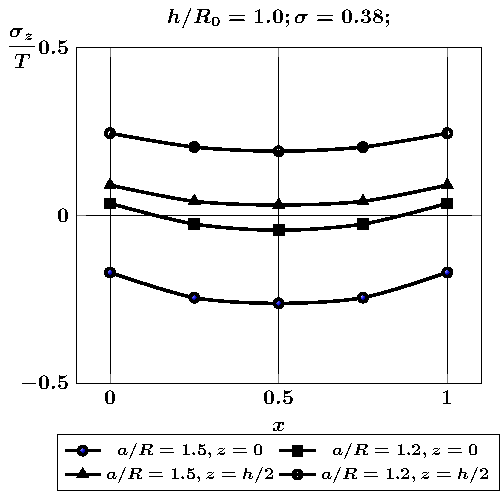
\includegraphics[width=7.5cm]{cav16-sig_z.pdf}
\caption{Напряжения $\sigma_z/T$ на линии $AB$ для конфигурации, представленной на рис.~\ref{f:7:27}, в зависимости от относительного расстояния между полостями в плоскостях $z=0$ и $z=h/2$
\label{f:7:30}}}\hfil\hfil
\parbox[b]{7.5cm}{\centering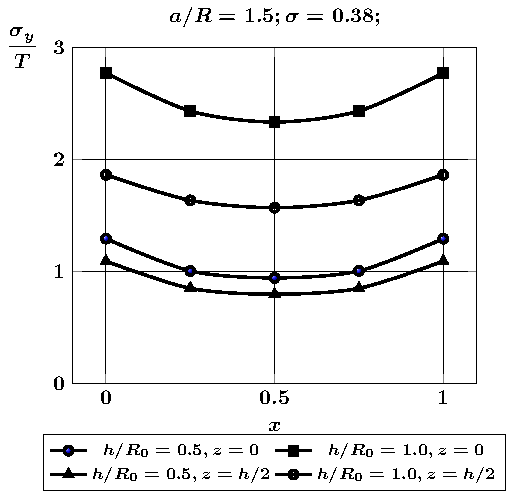
\includegraphics[width=7.5cm]{cav16-h-sig_y.pdf}
\caption{Напряжения $\sigma_y/T$ на линии $AB$ для конфигурации, представленной на рис.~\ref{f:7:27}, в зависимости от интенсивности приложенной внешней нагрузки $h/R_0$ в плоскостях $z=0$ и $z=h/2$
\label{f:7:31}}}
\end{figure}

\begin{figure}[h!]
\centering\footnotesize
\parbox[b]{7.5cm}{\centering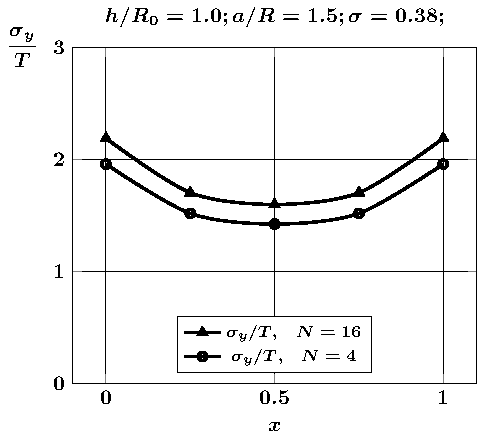
\includegraphics[width=7.5cm]{cav16-4-sig_y.pdf}
\caption{Напряжения $\sigma_y/T$ на линии $AB$ для конфигураций, представленных на рис.~\ref{f:7:6} и~\ref{f:7:27}, в зависимости от количества полостей в тетрагональной структуре
\label{f:7:32}}}\hfil\hfil
\parbox[b]{7.5cm}{\centering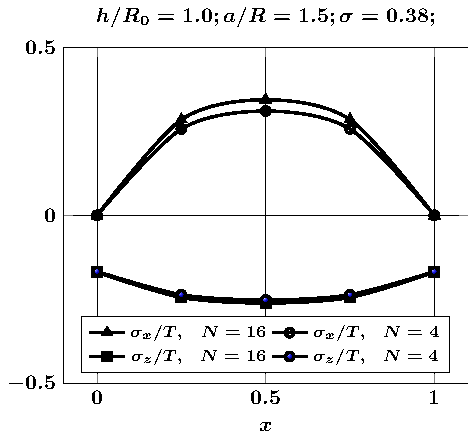
\includegraphics[width=7.5cm]{cav16-4-sig_x_z.pdf}
\caption{Напряжения $\sigma_x/T$ и $\sigma_z/T$ на линии $AB$ для конфигураций, представленных на рис.~\ref{f:7:6} и~\ref{f:7:27}, в зависимости от количества полостей в тетрагональной структуре
\label{f:7:33}}}
\end{figure}

\begin{table}[h!]
\caption{Сходимость метода редукции для случая шестнадцати полостей}
\centering
\begin{tabular}{|c|c|c|c|c|}
\hline
$m_{max}$ & 5 & 10 & 15 & 20 \\
\hline
$\sigma_x/T$ & $0.343729$ & $0.344384$ & $0.344381$ & $0.344382$ \\
\hline
$\sigma_y/T$ & $1.5964$ & $1.59645$ & $1.59648$ & $1.59648$ \\
\hline
$\sigma_z/T$ & $-0.260994$ & $-0.260695$ & $-0.260671$ & $-0.260669$ \\
\hline
\end{tabular}
\label{t:7:5}
\end{table}

На рис.~\ref{f:7:32} и~\ref{f:7:33} приведены графики напряжений $\sigma_x/T$, $\sigma_y/T$ и $\sigma_z/T$ на линии, соединяющей центры соседних полостей, для конфигураций, представленных на рис.~\ref{f:7:6} и~\ref{f:7:27}, в зависимости от количества полостей в тетрагональной структуре. Можно сделать вывод, что значения напряжений $\sigma_x/T$ и $\sigma_z/T$ и их распределения на линии $AB$ практически не зависят от числа полостей, в то время как напряжения $\sigma_y/T$ в случае шестнадцати полостей увеличиваются примерно на 10~\%. Характер распределения напряжений от числа полостей не зависит. Приведенные данные позволяют использовать локальные модели при описании напряженно-деформированного состояния пористого материала с параллельными цилиндрическими порами.

\subsection{Тетрагональная объемно центрированная структура расположения полостей в цилиндрическом образце}

%\sidefig(75mm){
%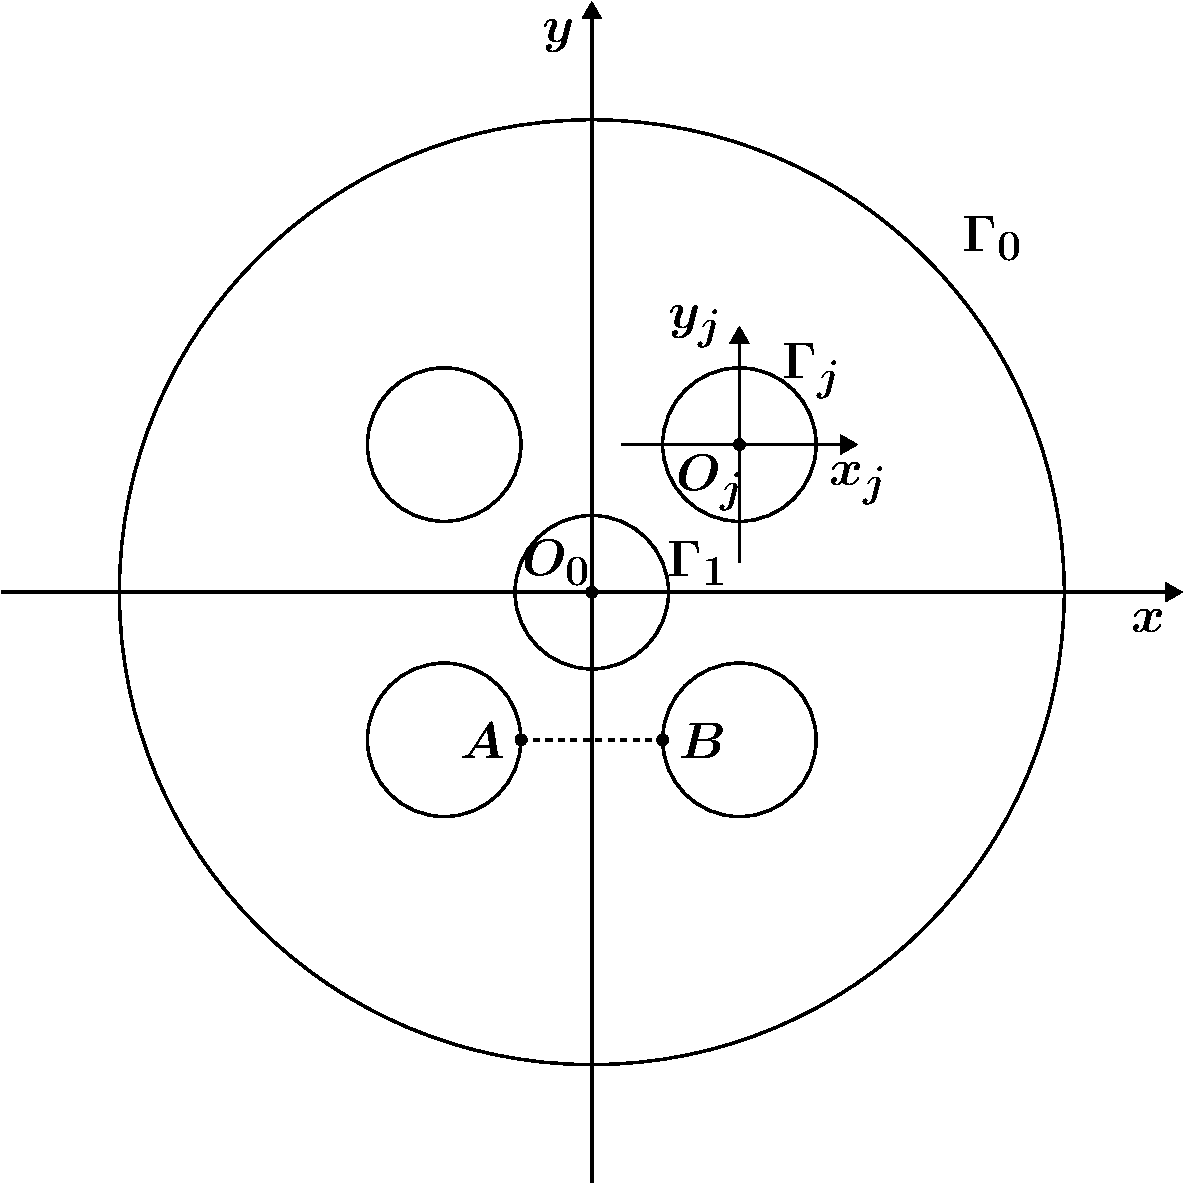
\includegraphics[width=7.5cm]{tetragonal-centroid.pdf}
%\caption{Тетрагональная объемно центрированная структура расположения полостей в цилиндрическом образце}
%\label{f:7:18}
%}{Рассмотрим тетрагональную объемно центрированную структуру расположения полостей в цилиндрическом образце, представленную на рис.~\ref{f:7:18}. Компьютерный эксперимент показывает качественно иной характер в распределении напряжений при переходе от тетрагональной упаковки к объемно центрированному ее варианту. Поэтому изучение такого вида упаковки является важным для оптимального определения геометрических параметров, приводящих к наименьшей концентрации напряжений в теле.
% 
%Заметим, что формулы~\eqref{eq:7:22}~--- \eqref{eq:7:24} из параграфа 2.2 отражают другую структуру разрешающей системы для определения неизвестных коэффициентов в общем решении.
%}

Рассмотрим тетрагональную объемно центрированную структуру расположения полостей в цилиндрическом образце, представленную на рис.~\ref{f:7:18}. Компьютерный эксперимент показывает качественно иной характер в распределении напряжений при переходе от тетрагональной упаковки к объемно центрированному ее варианту. Поэтому изучение такого вида упаковки является важным для оптимального определения геометрических параметров, приводящих к наименьшей концентрации напряжений в теле.

\begin{figure}[h!]
\centering
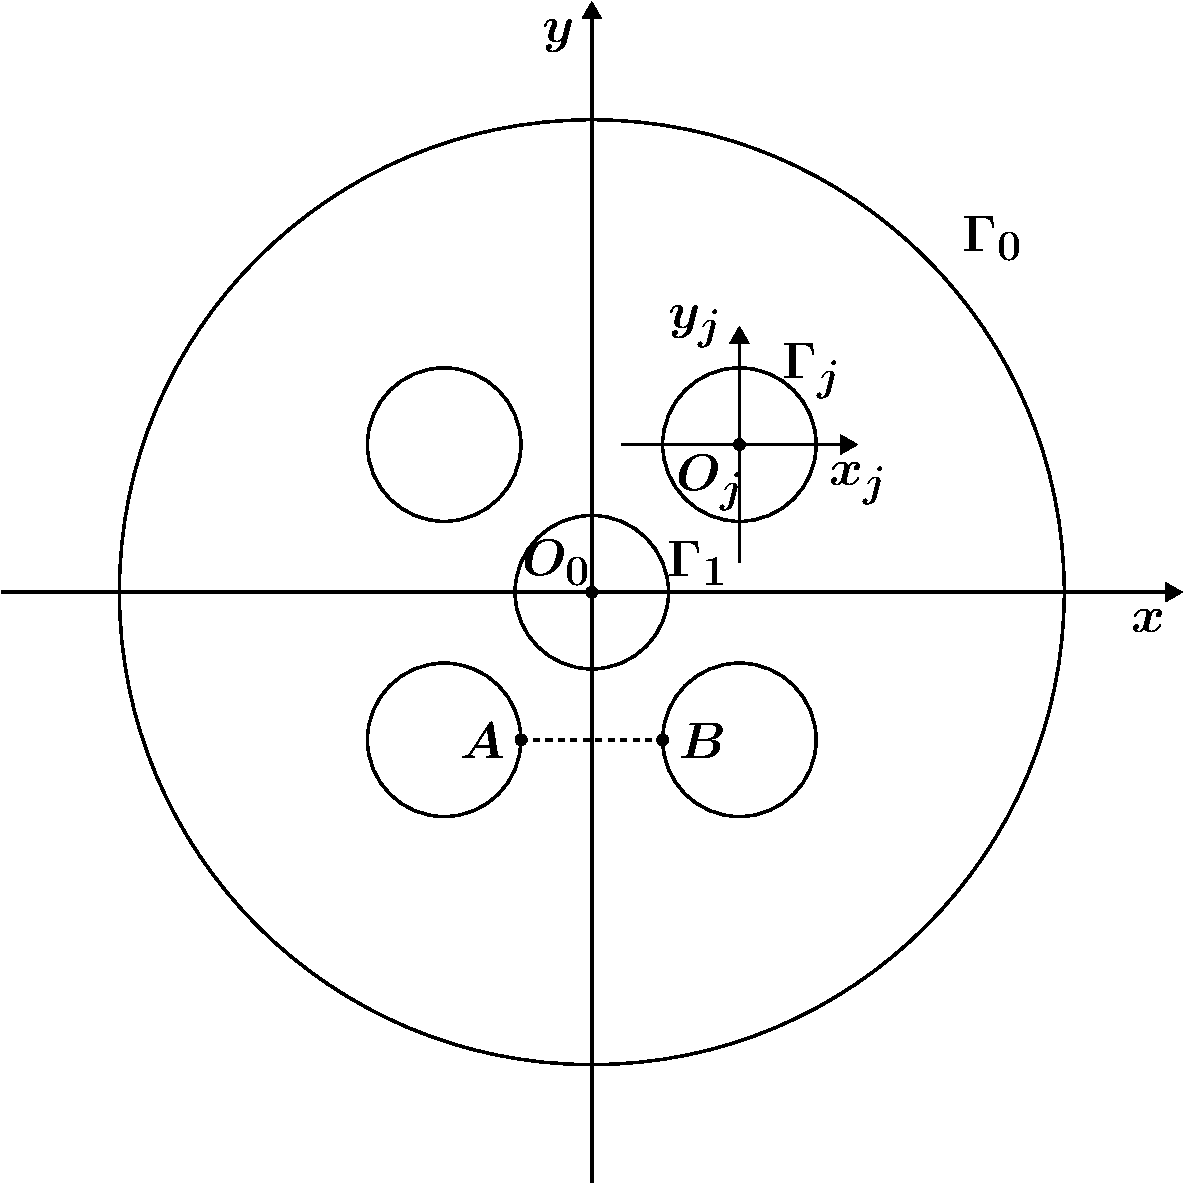
\includegraphics[width=8cm]{tetragonal-centroid.pdf}
\caption{Тетрагональная объемно центрированная структура расположения полостей в цилиндрическом образце}
\label{f:7:18}
\end{figure}
 
Заметим, что формулы~\eqref{eq:7:22}~--- \eqref{eq:7:24} из параграфа 2.2 отражают другую структуру разрешающей системы для определения неизвестных коэффициентов в общем решении.

На рис.~\ref{f:7:19} и~\ref{f:7:20} приводится сравнение относительных напряжений $\sigma_x/T$ и $\sigma_y/T$ на линии, соединяющей центры соседних полостей для тетрагональной и центрированной тетрагональной структур при прочих одинаковых параметрах.

\begin{figure}[h!]
\centering\footnotesize
\parbox[b]{7.5cm}{\centering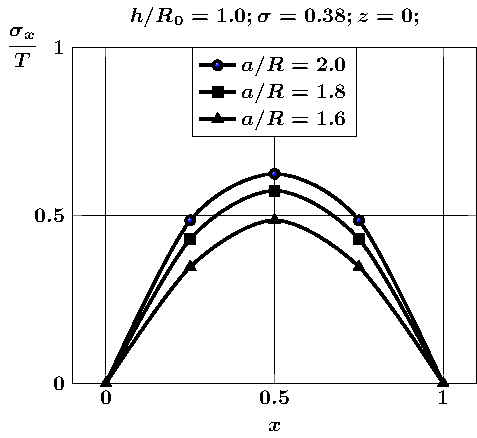
\includegraphics[width=7.5cm]{cav5-a-h10-r10-z0-sig_x.pdf}
\caption{Напряжения $\sigma_x/T$ на линии $AB$ для центрированной тетрагональной структуры в зависимости от относительного расстояния между полостями в плоскости $z=0$ 
\label{f:7:95}}}\hfil\hfil
\parbox[b]{7.5cm}{\centering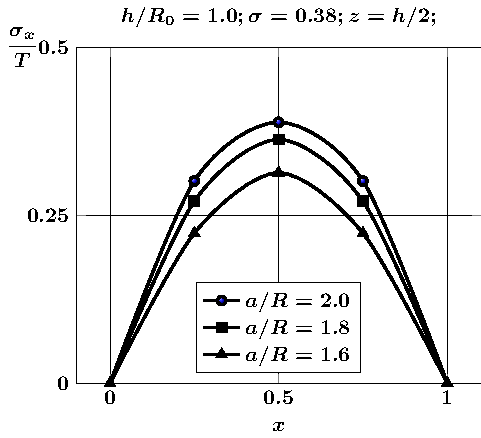
\includegraphics[width=7.5cm]{cav5-a-h10-r10-z1-sig_x.pdf}
\caption{Напряжения $\sigma_x/T$ на линии $AB$ для центрированной тетрагональной структуры в зависимости от относительного расстояния между полостями в плоскости $z=h/2$
\label{f:7:96}}}
\end{figure}

\begin{figure}[h!]
\centering\footnotesize
\parbox[b]{7.5cm}{\centering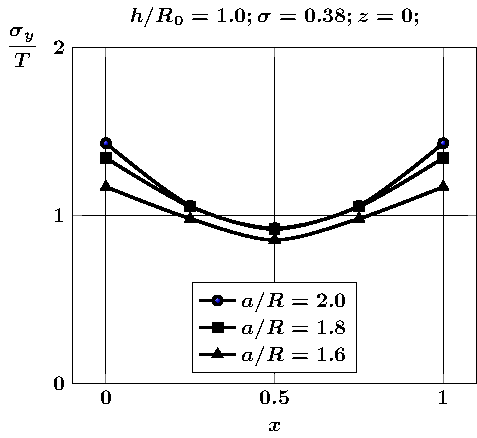
\includegraphics[width=7.5cm]{cav5-a-h10-r10-z0-sig_y.pdf}
\caption{Напряжения $\sigma_y/T$ на линии $AB$ для центрированной тетрагональной структуры в зависимости от относительного расстояния между полостями в плоскости $z=0$ 
\label{f:7:97}}}\hfil\hfil
\parbox[b]{7.5cm}{\centering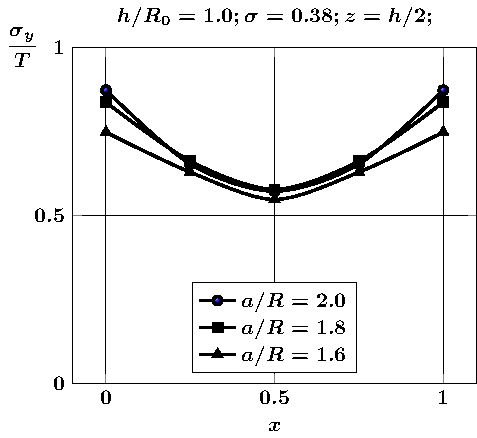
\includegraphics[width=7.5cm]{cav5-a-h10-r10-z1-sig_y.pdf}
\caption{Напряжения $\sigma_y/T$ на линии $AB$ для центрированной тетрагональной структуры в зависимости от относительного расстояния между полостями в плоскости $z=h/2$
\label{f:7:98}}}
\end{figure}

\begin{figure}[h!]
\centering\footnotesize
\parbox[b]{7.5cm}{\centering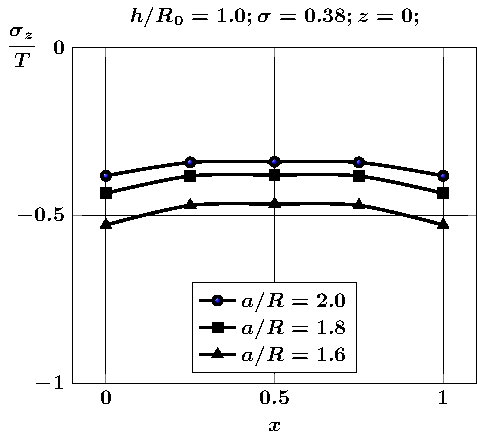
\includegraphics[width=7.5cm]{cav5-a-h10-r10-z0-sig_z.pdf}
\caption{Напряжения $\sigma_z/T$ на линии $AB$ для центрированной тетрагональной структуры в зависимости от относительного расстояния между полостями в плоскости $z=0$ 
\label{f:7:99}}}\hfil\hfil
\parbox[b]{7.5cm}{\centering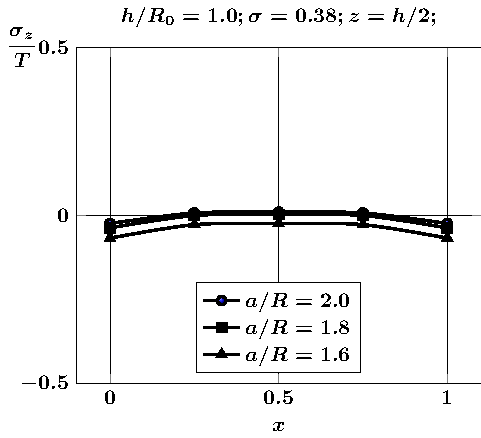
\includegraphics[width=7.5cm]{cav5-a-h10-r10-z1-sig_z.pdf}
\caption{Напряжения $\sigma_z/T$ на линии $AB$ для центрированной тетрагональной структуры в зависимости от относительного расстояния между полостями в плоскости $z=h/2$
\label{f:7:100}}}
\end{figure}

\begin{figure}[h!]
\centering\footnotesize
\parbox[b]{7.5cm}{\centering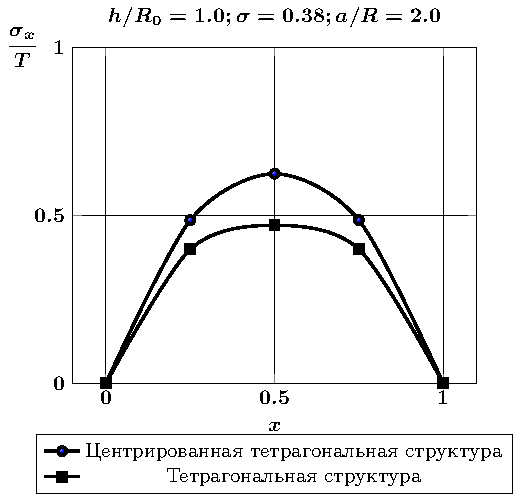
\includegraphics[width=7.5cm]{cav5-4-sig_x.pdf}
\caption{Напряжения $\sigma_x/T$ на линии $AB$ для тетрагональной и центрированной тетрагональной структур
\label{f:7:19}}}\hfil\hfil
\parbox[b]{7.5cm}{\centering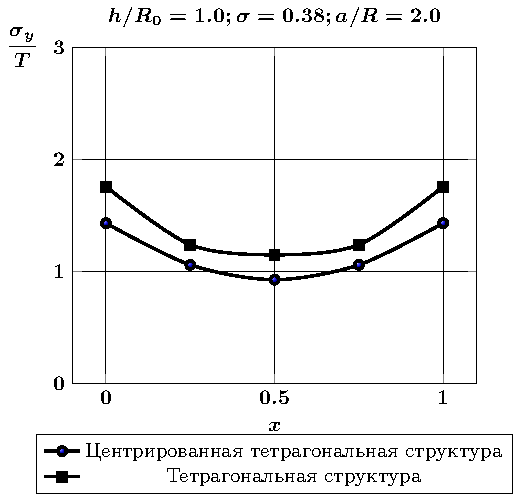
\includegraphics[width=7.5cm]{cav5-4-sig_y.pdf}
\caption{Напряжения $\sigma_y/T$ на линии $AB$ для тетрагональной и центрированной тетрагональной структур
\label{f:7:20}}}
\end{figure}

\subsection{Гексагональная структура расположения полостей в~цилиндрическом образце}

Рассмотрим гексагональную структуру расположения полостей в цилиндрическом образце, представленную на рис.~\ref{f:7:21}. Гексагональная упаковка обладает максимальной степенью симметрии по отношению к упаковкам, рассмотренным ранее. При вычислении эффективных упругих модулей для материала с подобным расположением полостей можно считать, что этот материал обладает трансверсальной изотропией при условии, что на его границе приложено однородное напряженно-деформированное состояние.

%\sidefig*(75mm){
%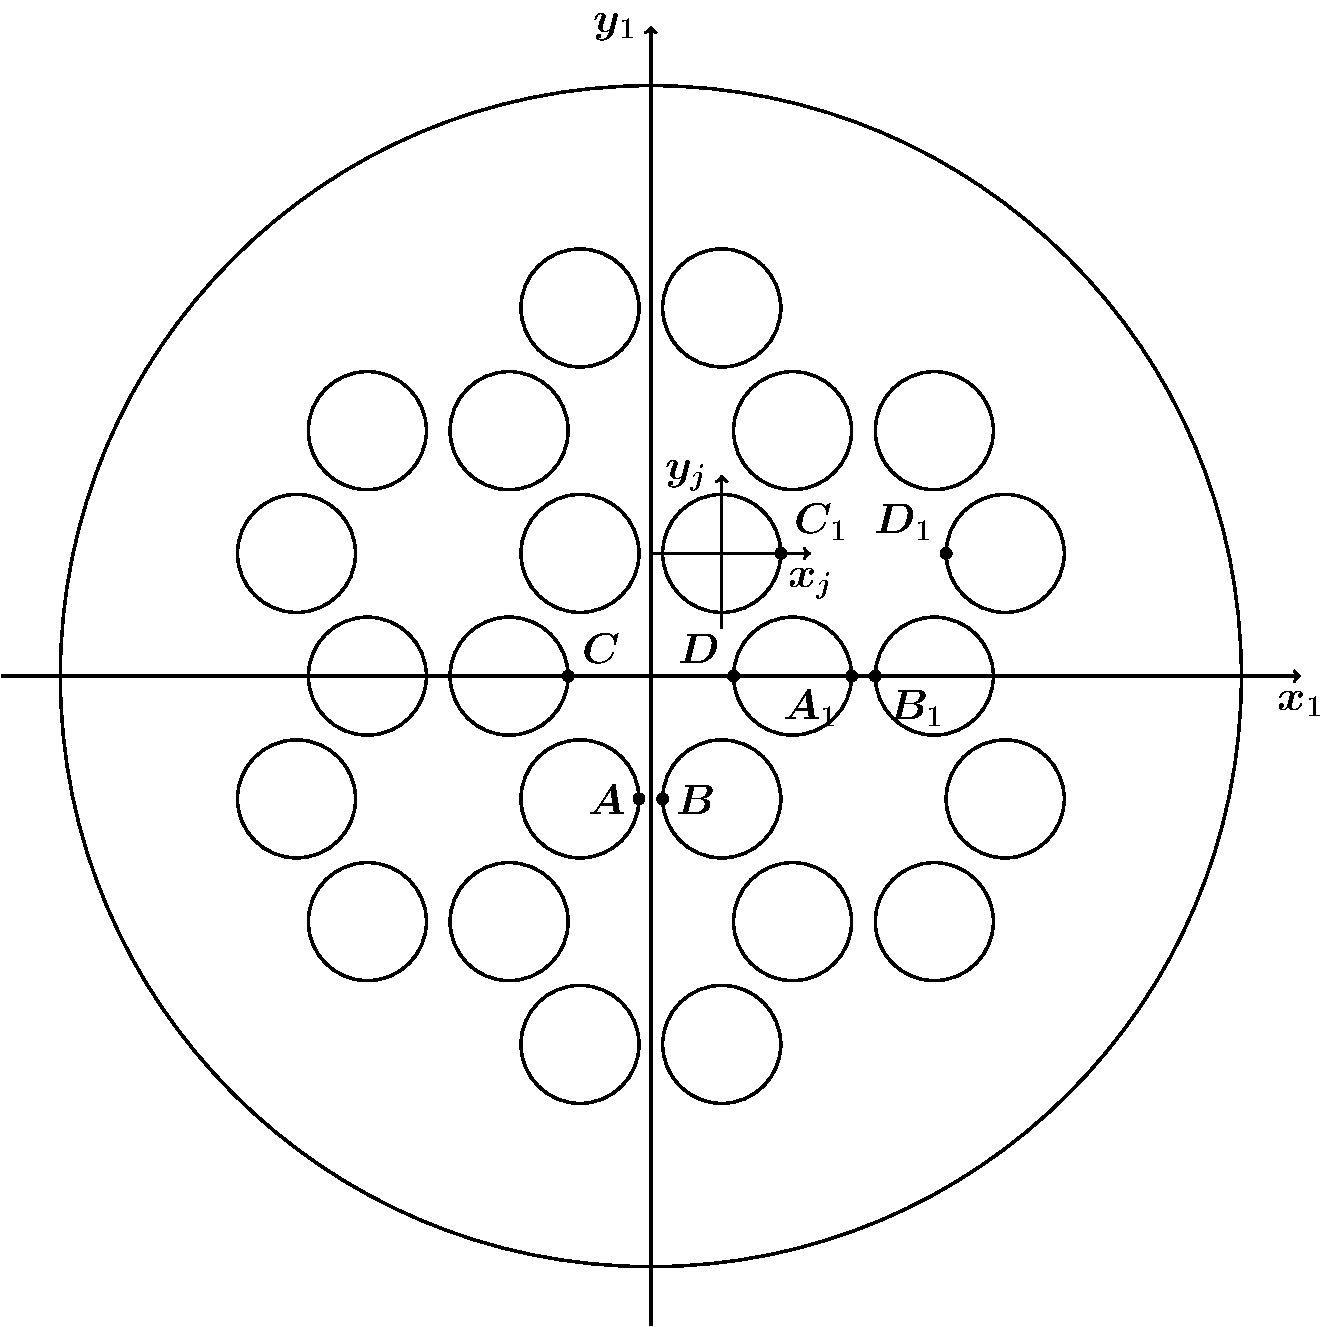
\includegraphics[width=7.5cm]{hexagonal.pdf}
%\caption{Гексагональная структура расположения полостей в цилиндрическом образце}
%\label{f:7:21}
%}

\begin{figure}[h!]
\centering
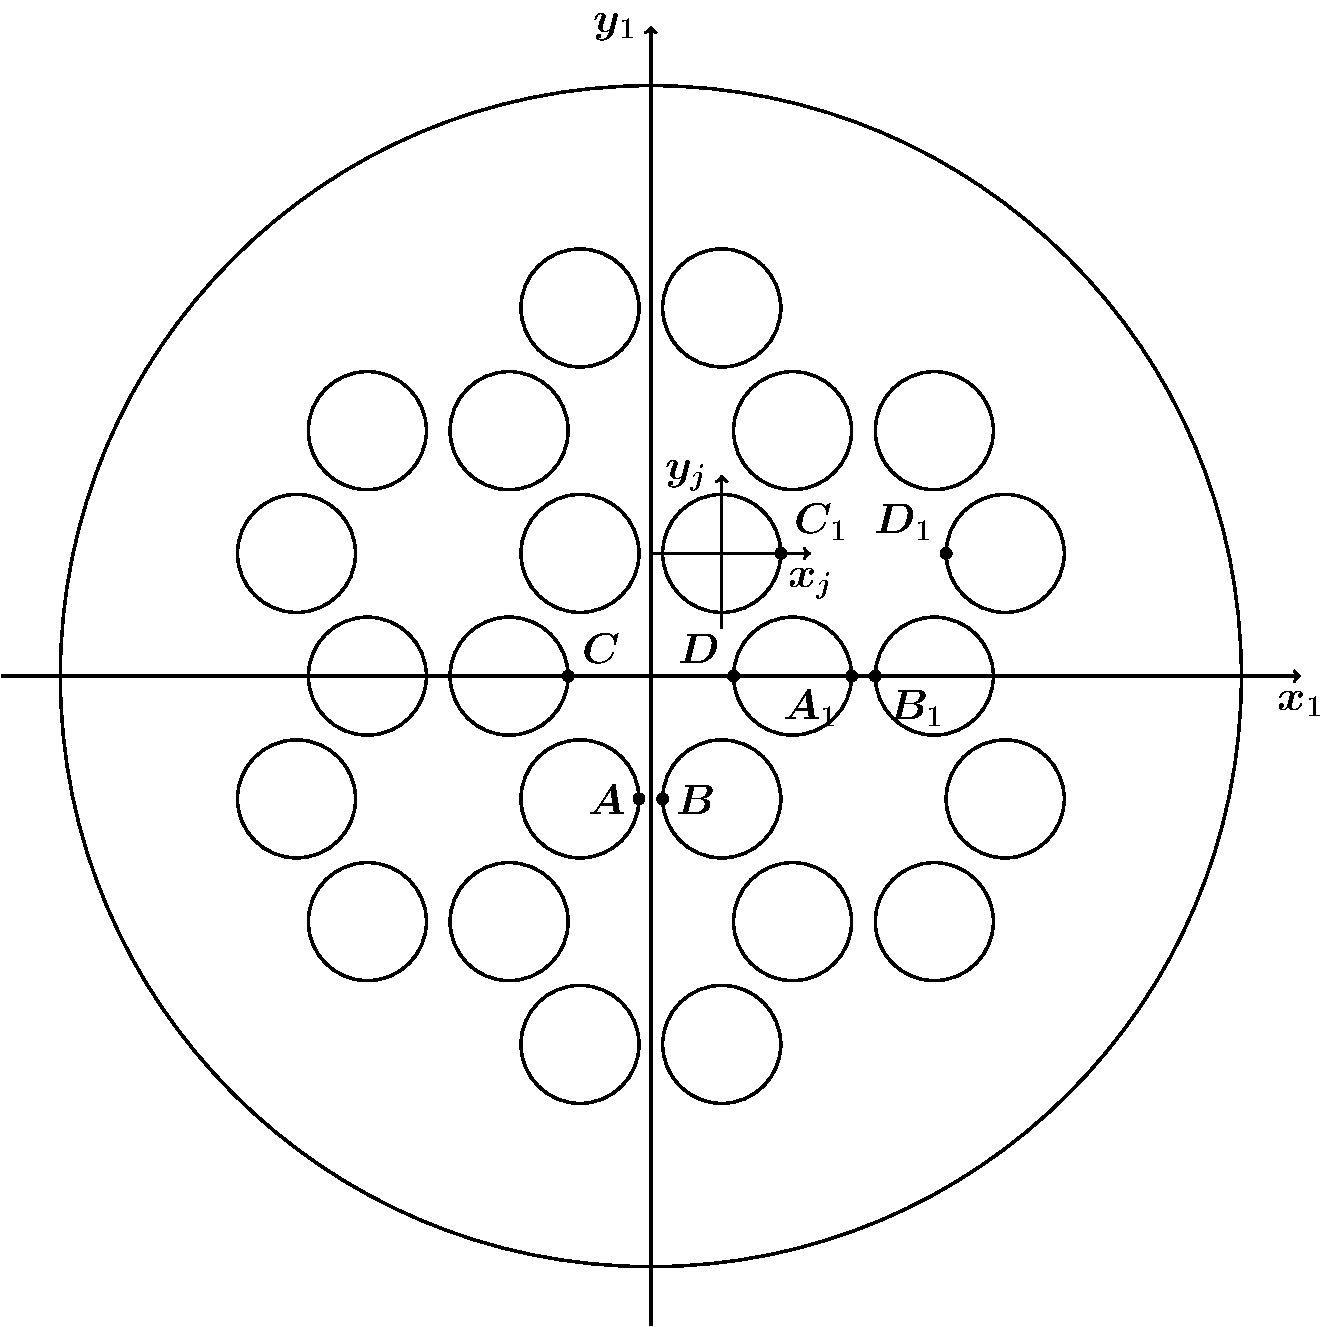
\includegraphics[width=7.5cm]{hexagonal.pdf}
\caption{Гексагональная структура расположения полостей в цилиндрическом образце}
\label{f:7:21}
\end{figure}

На рис.~\ref{f:7:126} и \ref{f:7:127} приведены графики нормальных напряжений на линии $AB$ в плоскостях $z=0$ и $z=h/2$ в зависимости от относительного расстояния между полостями. При уменьшении расстояния между полостями наблюдается рост напряжений $\sigma_y/T$. Для напряжений $\sigma_x/T$ наблюдается обратная картина. Напряжения $\sigma_z/T$ при приближении полостей меняют знак с сжимающих на растягивающие. Основной вклад в напряженное состояние вносят напряжения $\sigma_y/T$. На эти напряжения в наибольшей степени оказывает влияние расстояние между полостями.

\begin{figure}[h!]
\centering\footnotesize
\parbox[b]{7.5cm}{\centering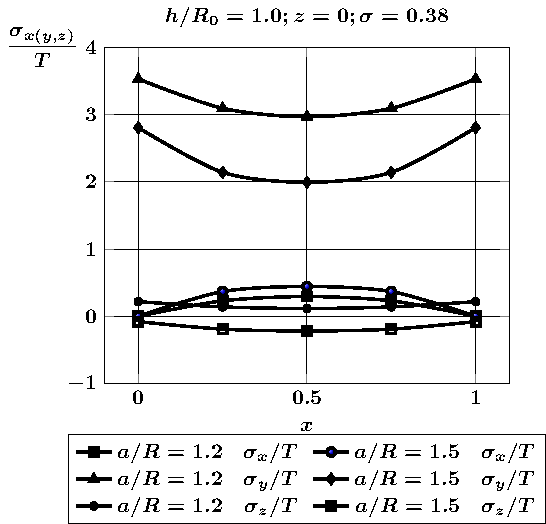
\includegraphics[width=8cm]{cav24-a-h10-r10-z0.pdf}
\caption{Нормальные напряжения на линии $AB$ в зависимости от относительного расстояния между полостями в плоскости $z=0$
\label{f:7:126}}}\hfil\hfil
\parbox[b]{7.5cm}{\centering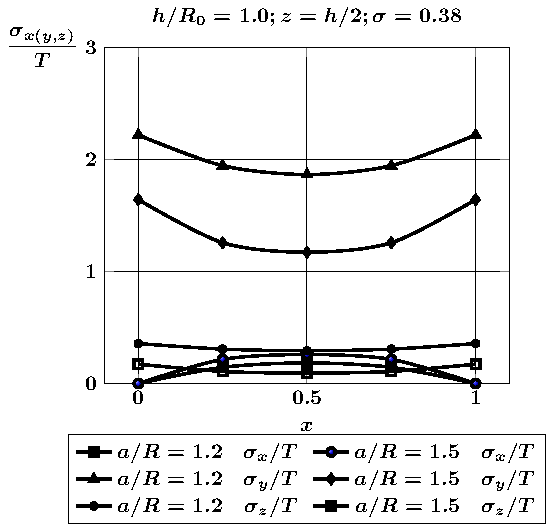
\includegraphics[width=8cm]{cav24-a-h10-r10-z1.pdf}
\caption{Нормальные напряжения на линии $AB$ в зависимости от относительного расстояния между полостями в плоскости $z=h/2$
\label{f:7:127}}}
\end{figure}

На рис.~\ref{f:7:128} и \ref{f:7:129} представлены графики нормальных напряжений на линии $CD$ в плоскостях $z=0$ и $z=h/2$ в зависимости от относительного расстояния между полостями. При уменьшении расстояния между полостями наблюдается уменьшение напряжений $\sigma_x/T$ и $\sigma_y/T$. Напряжения $\sigma_z/T$ растут по абсолютной величине при приближении полостей и являются сжимающими вне зависимости от расстояния между ними. В сравнении с отрезком $AB$ напряжения $\sigma_y/T$ на линии $CD$ уменьшаются в среднем в 2--2.5~раза.

\begin{figure}[h!]
\centering\footnotesize
\parbox[b]{7.5cm}{\centering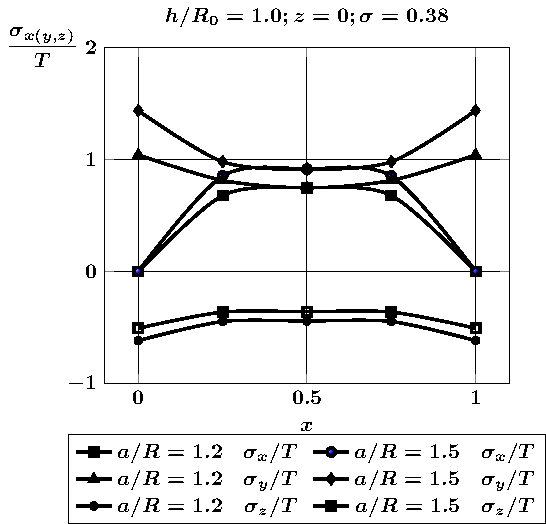
\includegraphics[width=8cm]{cav24-a-h10-r10-z0-diag.pdf}
\caption{Нормальные напряжения на линии $CD$ в зависимости от относительного расстояния между полостями в плоскости $z=0$
\label{f:7:128}}}\hfil\hfil
\parbox[b]{7.5cm}{\centering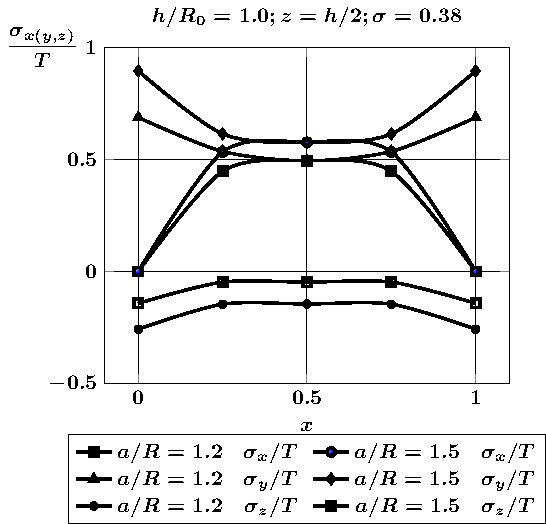
\includegraphics[width=8cm]{cav24-a-h10-r10-z1-diag.pdf}
\caption{Нормальные напряжения на линии $CD$ в зависимости от относительного расстояния между полостями в плоскости $z=h/2$
\label{f:7:129}}}
\end{figure}

В табл.~\ref{t:7:7} приведены результаты, показывающие скорость сходимости метода редукции для 24 цилиндрических полостей. Сравниваются значения напряжений $\sigma_x/T$, $\sigma_y/T$, $\sigma_z/T$ в средней точке отрезка $AB$ при $m_{max}=10,12,15$, $a/R=1.5$, $h/R_0=1.0$. Метод показал хорошую сходимость уже для $m_{max}=10$.\par\sloppy

\begin{table}[h!]
\caption{Сходимость метода редукции для 24 цилиндрических полостей}
\centering
$
\begin{array}{|c|c|c|c|}
\hline
m_{max} & 10 & 12 & 15 \\
\hline
\sigma_x & 0.441673 & 0.440023 & 0.440023 \\
\hline
\sigma_y & 1.9923 & 1.98469 & 1.98469 \\
\hline
\sigma_z & -0.219197 & -0.219834 & -0.219834 \\
\hline
\end{array}
$
\label{t:7:7}
\end{table}

\begin{figure}[h!]
\centering\footnotesize
\parbox[b]{7.5cm}{\centering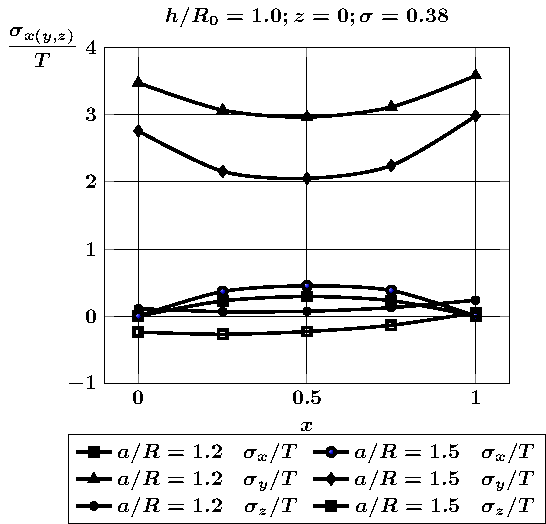
\includegraphics[width=8cm]{cav24-a-h10-r10-z0-a1b1.pdf}
\caption{Нормальные напряжения на линии $A_1B_1$ в зависимости от относительного расстояния между полостями в плоскости $z=0$
\label{f:7:130}}}\hfil\hfil
\parbox[b]{7.5cm}{\centering\includegraphics[width=8cm]{cav24-a-h10-r10-z0-c1d1.pdf}
\caption{Нормальные напряжения на линии $C_1D_1$ в зависимости от относительного расстояния между полостями в плоскости $z=0$
\label{f:7:131}}}
\end{figure}

\begin{figure}[h!]
\centering\footnotesize
\parbox[b]{7.5cm}{\centering\includegraphics[width=8cm]{cav24-6-a12-h10-r10-z0.pdf}
\caption{Нормальные напряжения на линии $AB$ для гексагональной структуры при 6 и 24 полостях
\label{f:7:132}}}\hfil\hfil
\parbox[b]{7.5cm}{\centering\includegraphics[width=8cm]{cav24-6-a12-h10-r10-z0-diag.pdf}
\caption{Нормальные напряжения на линии $CD$ для гексагональной структуры при 6 и 24 полостях
\label{f:7:133}}}
\end{figure}

На рис.~\ref{f:7:130} и \ref{f:7:131} приведены графики нормальных напряжений на линиях $A_1B_1$ и $C_1D_1$ в плоскости $z=0$ в зависимости от относительного расстояния между полостями. При сохранении характера распределения напряжений по сравнению с центрально расположенной ячейкой наблюдается характерная асимметрия поля напряжений относительно срединных точек отрезков.

На рис.~\ref{f:7:132} и~\ref{f:7:133} приводится сравнение нормальных напряжений на линиях $AB$ и $CD$ в зависимости от количества ячеек в гексагональной упаковке. Заметное отличие наблюдается для напряжений $\sigma_y/T$ на отрезке $AB$ и напряжений $\sigma_x/T$ и $\sigma_y/T$ на отрезке $CD$.

\subsection{Гексагональная центрированная структура расположения полостей в цилиндрическом образце}

\sidefig(75mm){
\includegraphics[width=7.5cm]{hexagonal-centroid.pdf}
\caption{Гексагональная центрированная структура расположения полостей в цилиндрическом образце}
\label{f:7:24}
}{Рассмотрим гексагональную центрированную структуру расположения полостей в цилиндрическом образце, представленную на рис.~\ref{f:7:24}. Эта структура соответствует наибольшему объемному содержанию пор в пористом материале.

На рис.~\ref{f:7:134} и~\ref{f:7:135} приводятся графики нормальных напряжений на линии $AB$ в плоскостях $z=0$ и $z=h/2$ в зависимости от относительного расстояния $a/R$ между полостями. Наибольший вклад в тензор напряжений вносят напряжения $\sigma_y/T$, которые растут с приближением полостей друг к другу. Область их концентрации расположена вблизи границ полостей.} 

Напряжения $\sigma_x/T$, напротив, растут с увеличением расстояния между полостями.

\begin{figure}[h!]
\centering\footnotesize
\parbox[b]{7.5cm}{\centering\includegraphics[width=8cm]{cav31-a-h10-r10-z0.pdf}
\caption{Нормальные напряжения на линии $AB$ в зависимости от относительного расстояния между полостями в плоскости $z=0$
\label{f:7:134}}}\hfil\hfil
\parbox[b]{7.5cm}{\centering\includegraphics[width=8cm]{cav31-a-h10-r10-z1.pdf}
\caption{Нормальные напряжения на линии $AB$ в зависимости от относительного расстояния между полостями в плоскости $z=h/2$
\label{f:7:135}}}
\end{figure}

Напряжения $\sigma_z/T$ всюду на отрезке $AB$ в плоскости $z=0$ являются сжимающими и практически постоянны. Напряжения $\sigma_x/T$, $\sigma_z/T$ на отрезке $AB$ в плоскости $z=h/2$ в 1.5--2 раза меньше, чем в плоскости $z=0$. При этом характер их распределения остается тем же.

\begin{figure}[h!]
\centering\footnotesize
\parbox[b]{7.5cm}{\centering\includegraphics[width=7.8cm]{cav31-a-h10-r10-z0-a1b1.pdf}
\caption{Нормальные напряжения на линии $A_1B_1$ в зависимости от относительного расстояния между полостями в плоскости $z=0$
\label{f:7:136}}}\hfil\hfil
\parbox[b]{7.5cm}{\centering\includegraphics[width=7.8cm]{cav31-a-h10-r10-z1-a1b1.pdf}
\caption{Нормальные напряжения на линии $A_1B_1$ в зависимости от относительного расстояния между полостями в плоскости $z=h/2$
\label{f:7:137}}}
\end{figure}

\begin{figure}[h!]
\centering\footnotesize
\parbox[b]{7.5cm}{\centering\includegraphics[width=7.8cm]{cav31-24-a12-h10-r10-z0.pdf}
\caption{Сравнение нормальных напряжений на линии $AB$ для гексагональной и центрированной гексагональной упаковок при $a/R=1.2$
\label{f:7:138}}}\hfil\hfil
\parbox[b]{7.5cm}{\centering\includegraphics[width=7.8cm]{cav31-24-a15-h10-r10-z0.pdf}
\caption{Сравнение нормальных напряжений на линии $AB$ для гексагональной и центрированной гексагональной упаковок при $a/R=1.5$
\label{f:7:139}}}
\end{figure}

\begin{figure}[h!]
\centering\footnotesize
\parbox[b]{7.5cm}{\centering\includegraphics[width=7.5cm]{cav7-5-sig_x.pdf}
\caption{Напряжения $\sigma_x/T$ на линии, соединяющей центры соседних полостей, для гексагональной и тетрагональной центрированных структур
\label{f:7:25}}}\hfil\hfil
\parbox[b]{7.5cm}{\centering\includegraphics[width=7.5cm]{cav7-5-sig_y.pdf}
\caption{Напряжения $\sigma_y/T$ на линии, соединяющей центры соседних полостей, для гексагональной и тетрагональной центрированных структур
\label{f:7:26}}}
\end{figure}

На рис.~\ref{f:7:136} и~\ref{f:7:137} представлены графики нормальных напряжений на линии $A_1B_1$ в плоскостях $z=0$ и $z=h/2$ в зависимости от относительного расстояния $a/R$ между полостями.

Наблюдаются те же особенности в распределении напряжений, что и для отрезка $AB$, с характерной асимметрией, которая имеет место для смещенной относительно центра образца ячейки.

На рис.~\ref{f:7:138} и~\ref{f:7:139} приведено сравнение нормальных напряжений на линии $AB$ для гексагональной и центрированной гексагональной упаковок в плоскости $z=0$ при $a/R=1.2$ и $a/R=1.5$. Интересно отметить, что в центрированном случае, при большем объемном содержании пор, напряжения $\sigma_y/T$ примерно на 20~\% меньше, чем в нецентрированном случае. По-видимому, это обусловлено более равномерным распределением напряжений по ячейке в центрированной структуре, чем в нецентрированной.

На рис.~\ref{f:7:25} и~\ref{f:7:26} показано сравнение относительных напряжений $\sigma_x/T$ и $\sigma_y/T$ на линии $AB$ в случае одной ячейки для гексагональной и тетрагональной центрированных структур при $a/R=2.0$ в плоскости $z=0$. Характер распределения напряжений показывает, что гексагональная центрированная ячейка в силу большей симметрии более равномерно перераспределяет напряжения по ячейке, поэтому максимальные значения рассматриваемых напряжений в гексагональном случае ниже, чем в тетрагональном.

Можно сделать вывод, что структура материала оказывает влияние на численные значения нормальных напряжений, которые возникают в материале под действием внешней нагрузки.

\section{Упругое состояние композита с линейной регулярной структурой}

\sidefig*(75mm){
\includegraphics[width=7.5cm]{incl-scheme.pdf}
\caption{Схематическое представление задачи}
\label{f:7:34}
}{Рассмотрим цилиндрический образец однонаправленного волокнистого композиционного материала. Включения имеют форму бесконечных круговых цилиндров радиуса $R_\alpha$. Представительскую ячейку материала будем характеризовать расположением центров $\{O_j\}_{j=1}^N$ круговых сечений волокон плоскостью, перпендикулярной оси образца. Пусть $O_0$~--- центр представительской ячейки. Если ячейка объемно центрирована, то считаем, что $O_0$ совпадает с $O_1$, в противном случае $O_0$ не совпадает с $O_1$ $(j=\overline{1,N})$ (рис.~\ref{f:7:34}).}

Будем считать, что упругие постоянные матрицы и включений равны $(\sigma_0, G_0)$, $(\sigma_j,G_j)$ соответственно. Предполагается, что к внешней границе цилиндра приложена ку\-соч\-но-пос\-то\-ян\-ная радиальная нагрузка.

Введем цилиндрические системы координат $(\rho_j,\varphi_j,z_j)$ c началами в точках $O_j$, оси $O_jz_j$ которых совпадают с осями цилиндров. Координаты в введенных системах координат связаны соотношениями~\eqref{eq:7:25}, \eqref{eq:7:26}.

Цилиндрический образец представляем как объединение областей матрицы $\Omega_0$ и включений $\Omega_j$. Обозначим через $\Gamma_0$ и $\Gamma_j$ внешнюю границу области $\Omega_0$ и границу $\Omega_j$.

Для определения НДС в рассматриваемом теле необходимо решить краевую задачу для уравнения Ламе~\eqref{eq:7:27} с граничным условием~\eqref{eq:7:19} и условиями сопряжения на границах включений

\begin{equation}
\left.\mathbf{U}^+\right|_{\Gamma_j}=\left.\mathbf{U}_j\right|_{\Gamma_j},
\label{eq:7:33}
\end{equation}

\begin{equation}
\left.\mathbf{FU}^+\right|_{\Gamma_j}=\left.\mathbf{FU}_j\right|_{\Gamma_j},
\label{eq:7:34}
\end{equation}

\noindent где $\mathbf{U}^+$~--- вектор перемещений в матрице; $\mathbf{U}_j$~--- вектор перемещений в $j$-м волокне; $\mathbf{FU}$~--- отвечающий $\mathbf{U}$ вектор усилий на соответствующей граничной поверхности; границы цилиндров $\Gamma_j$ задаются уравнениями $\rho_j=R_j$ ($j=\\=\overline{1,N}$).\par\sloppy

Решение задачи будем искать в виде

\begin{multline}
{{\bf{U}}^ + } = \sum\limits_{j = 1}^N {\sum\limits_{s = 1}^3 {\sum\limits_{m =  - \infty }^\infty  {\int\limits_{ - \infty }^\infty  {A_{s,m}^{(j)}} } } } (\lambda ){\bf{U}}_{s,\lambda ,m}^{ + (3)}\left( {{\rho _j},{z_j},{\varphi _j}} \right)d\lambda  + \\
+ \sum\limits_{s = 1}^3 {\sum\limits_{m =  - \infty }^\infty  {\mathop \smallint \limits_{ - \infty }^\infty  } } A_{s,m}^{(0)}(\lambda ){\bf{U}}_{s,\lambda ,m}^{ - (3)}\left( {{\rho _1},{z_1},{\varphi _1}} \right)d\lambda \;\;\;{\mkern 1mu} {\kern 1pt} {\kern 1pt} \left( {x,y,z} \right) \in {\Omega _0},
\end{multline}

\begin{equation}
{{\bf{U}}_j} = \sum\limits_{s = 1}^3 {\sum\limits_{m =  - \infty }^\infty  {\int\limits_{ - \infty }^\infty  {B_{s,m}^{(j)}} } } (\lambda ){\bf{U}}_{s,\lambda ,m}^{ - (3)}\left( {{\rho _j},{z_j},{\varphi _j}} \right)d\lambda \;\;\;{\mkern 1mu} {\kern 1pt} \left( {x,y,z} \right) \in {\Omega _j},
\end{equation}

\noindent где $A_{s,m}^{(j)}$, $B_{s,m}^{(j)}$~--- неизвестные функции; $\mathbf{U}_{s,\lambda,m}^{\pm(3)}(\rho,\varphi,z)$ определены в~\eqref{eq:7:1}, \eqref{eq:7:2}.

Используя теоремы сложения~\eqref{eq:7:7}~--- \eqref{eq:7:12}, представим вектор перемещения $\mathbf{U}^+$ в каждой из цилиндрических систем координат с центрами $O_j$ $(j=0\div N)$.

В случае, если ячейка не является объемно центрированной,
	
\begin{multline}
{{\bf{U}}^ + } = \sum\limits_{s = 1}^3 {\sum\limits_{m =  - \infty }^\infty  {\int\limits_{ - \infty }^\infty  \bigg\{  } } A_{s,m}^{(0)}(\lambda ){\bf{U}}_{s,\lambda ,m}^{ - (3)}({\rho _0},{z_0},{\varphi _0}) + {\bf{U}}_{s,\lambda ,m}^{ + (3)}({\rho _0},{z_0},{\varphi _0}) \times \\
\times \sum\limits_{\alpha  = 1}^N {\sum\limits_{t = 1}^3 {\sum\limits_{l =  - \infty }^\infty  {A_{t,l}^{(\alpha )}} } } (\lambda )\bigg[{\delta _{st}} + {\delta _{s1}}{\delta _{t2}}{\rho _{0\alpha }}\frac{\partial }{{\partial {\rho _{0\alpha }}}}\bigg]u_{\lambda ,l - m}^{ - (3)}({\rho _{0\alpha }},0,{\varphi _{0\alpha }})\bigg\} d\lambda,
\label{eq:7:28}
\end{multline}

\begin{multline}
{{\bf{U}}^ + } = \sum\limits_{s = 1}^3 {\sum\limits_{m =  - \infty }^\infty  {\int\limits_{ - \infty }^\infty  \bigg\{  } } A_{s,m}^{(\alpha )}(\lambda ){\bf{U}}_{s,\lambda ,m}^{ + (3)}({\rho _\alpha },{z_\alpha },{\varphi _\alpha }) + {\bf{U}}_{s,\lambda ,m}^{ - (3)}({\rho _\alpha },{z_\alpha },{\varphi _\alpha }) \times \\
\times \sum\limits_{t = 1}^3 {\sum\limits_{l =  - \infty }^\infty  {A_{t,l}^{(0)}} } (\lambda )\bigg[{\delta _{st}} + {\delta _{s1}}{\delta _{t2}}{\rho _{0\alpha }}\frac{\partial }{{\partial {\rho _{0\alpha }}}}\bigg]u_{\lambda ,l - m}^{ - (3)}({\rho _{0\alpha }},0,{\varphi _{0\alpha }}) + \\
+ \sum\limits_{j \ne \alpha } {{\bf{U}}_{s,\lambda ,m}^{ - (3)}} ({\rho _\alpha },{z_\alpha },{\varphi _\alpha })\sum\limits_{t = 1}^3 {\sum\limits_{l =  - \infty }^\infty  {A_{t,l}^{(j)}} } (\lambda ){( - 1)^m}\bigg[{\delta _{st}} + {\delta _{s1}}{\delta _{t2}}{\rho _{j\alpha }}\frac{\partial }{{\partial {\rho _{j\alpha }}}}\bigg] \times \\
\times u_{\lambda ,l - m}^{ + (3)}({\rho _{j\alpha }},0,{\varphi _{j\alpha }})\bigg\} d\lambda.
\label{eq:7:29}
\end{multline}

В случае объемно центрированной ячейки вектор перемещения имеет вид

\begin{multline}
{{\bf{U}}^ + } = \sum\limits_{s = 1}^3 {\sum\limits_{m =  - \infty }^\infty  {\int\limits_{ - \infty }^\infty  \bigg\{  } } A_{s,m}^{(0)}(\lambda ){\bf{U}}_{s,\lambda ,m}^{ - (3)}({\rho _1},{z_1},{\varphi _1}) + \\
+ A_{s,m}^{(1)}(\lambda ){\bf{U}}_{s,\lambda ,m}^{ + (3)}({\rho _1},{z_1},{\varphi _1}) + {\bf{U}}_{s,\lambda ,m}^{ + (3)}({\rho _1},{z_1},{\varphi _1})\sum\limits_{\alpha  = 2}^N {\sum\limits_{t = 1}^3 {\sum\limits_{l =  - \infty }^\infty  {A_{t,l}^{(\alpha )}} } } (\lambda )\bigg[{\delta _{st}} + \\
+ {\delta _{s1}}{\delta _{t2}}{\rho _{1\alpha }}\frac{\partial }{{\partial {\rho _{1\alpha }}}}\bigg]u_{\lambda ,l - m}^{ - (3)}({\rho _{1\alpha }},0,{\varphi _{1\alpha }})\bigg\} d\lambda,
\label{eq:7:30}
\end{multline}

\begin{multline}
{{\bf{U}}^ + } = \sum\limits_{s = 1}^3 {\sum\limits_{m =  - \infty }^\infty  {\int\limits_{ - \infty }^\infty  \bigg\{  } } A_{s,m}^{(0)}(\lambda ){\bf{U}}_{s,\lambda ,m}^{ - (3)}({\rho _1},{z_1},{\varphi _1}) + A_{s,m}^{(1)}(\lambda ){\bf{U}}_{s,\lambda ,m}^{ + (3)}({\rho _1},{z_1},{\varphi _1}) + \\
+ {\bf{U}}_{s,\lambda ,m}^{ - (3)}({\rho _1},{z_1},{\varphi _1})\sum\limits_{\alpha  = 2}^N {\sum\limits_{t = 1}^3 {\sum\limits_{l =  - \infty }^\infty  {A_{t,l}^{(\alpha )}} } } (\lambda ){( - 1)^l}\bigg[{\delta _{st}} + \\
+ {\delta _{s1}}{\delta _{t2}}{\rho _{1\alpha }}\frac{\partial }{{\partial {\rho _{1\alpha }}}}\bigg]u_{\lambda ,l - m}^{ + (3)}({\rho _{1\alpha }},0,{\varphi _{1\alpha }})\bigg\} d\lambda,
\label{eq:7:31}
\end{multline}

\begin{multline}
{\bf{U}} = \sum\limits_{s = 1}^3 {\sum\limits_{m =  - \infty }^\infty  {\int\limits_{ - \infty }^\infty  \bigg\{  } } A_{s,m}^{(\alpha )}(\lambda ){\bf{U}}_{s,\lambda ,m}^{ + (3)}({\rho _\alpha },{z_\alpha },{\varphi _\alpha }) + {\bf{U}}_{s,\lambda ,m}^{ - (3)}({\rho _\alpha },{z_\alpha },{\varphi _\alpha }) \times \\
\times \sum\limits_{t = 1}^3 {\sum\limits_{l =  - \infty }^\infty  {A_{t,l}^{(0)}} } (\lambda )\bigg[{\delta _{st}} + {\delta _{s1}}{\delta _{t2}}{\rho _{0\alpha }}\frac{\partial }{{\partial {\rho _{0\alpha }}}}\bigg]u_{\lambda ,l - m}^{ - (3)}({\rho _{0\alpha }},0,{\varphi _{0\alpha }}) + \\
+ \sum\limits_{j \ne \alpha } {{\bf{U}}_{s,\lambda ,m}^{ - (3)}} ({\rho _\alpha },{z_\alpha },{\varphi _\alpha })\sum\limits_{t = 1}^3 {\sum\limits_{l =  - \infty }^\infty  {A_{t,l}^{(j)}} } (\lambda ){( - 1)^m}\bigg[{\delta _{st}} + {\delta _{s1}}{\delta _{t2}}{\rho _{j\alpha }}\frac{\partial }{{\partial {\rho _{j\alpha }}}}\bigg] \times \\
\times u_{\lambda ,l - m}^{ + (3)}({\rho _{j\alpha }},0,{\varphi _{j\alpha }})\bigg\} d\lambda ,\qquad {\kern 1pt} \alpha  \ne 1.
\label{eq:7:32}
\end{multline}

Используя формулы~\eqref{eq:7:28}~--- \eqref{eq:7:32}, в результате удовлетворения граничным условиям~\eqref{eq:7:19} и условиям сопряжения~\eqref{eq:7:33}, \eqref{eq:7:34} для случая необъемно центрированной ячейки получаем бесконечную систему линейных алгебраических уравнений относительно неизвестных функций $A_{s,m}^{(j)}(\lambda)$, $B_{s,m}^{(j)}(\lambda)$:

\begin{multline}
\sum\limits_{s = 1}^3 \bigg\{  A_{s,m}^{(0)}(\lambda ){\bf{G}}_{s,\lambda ,m}^{ - (3)}({R_0},{G_0},{\sigma _0}) + {\bf{G}}_{s,\lambda ,m}^{ + (3)}({R_0},{G_0},{\sigma _0}) \times \\
\times \sum\limits_{\alpha  = 1}^N {\sum\limits_{t = 1}^3 {\sum\limits_{l =  - \infty }^\infty  {A_{t,l}^{(\alpha )}} } } (\lambda )\bigg[{\delta _{st}} + {\delta _{s1}}{\delta _{t2}}{\rho _{1\alpha }}\frac{\partial }{{\partial {\rho _{1\alpha }}}}\bigg]u_{\lambda ,l - m}^{ - (3)}({\rho _{1\alpha }},0,{\varphi _{1\alpha }})\bigg\}  = \\
= \frac{T}{\pi }\frac{{\sin \lambda h}}{\lambda }{\delta _{m0}}(1,1,0),
\end{multline}

\begin{multline}
\sum\limits_{s = 1}^3 \bigg\{  A_{s,m}^{(\alpha )}(\lambda ){\bf{H}}_{s,\lambda ,m}^{ + (3)}({R_\alpha },{\sigma _0}) + {\bf{H}}_{s,\lambda ,m}^{ - (3)}({R_\alpha },{\sigma _0}) \times \\
\times \sum\limits_{t = 1}^3 {\sum\limits_{l =  - \infty }^\infty  {A_{t,l}^{(1)}} } (\lambda )\bigg[{\delta _{st}} + {\delta _{s1}}{\delta _{t2}}{\rho _{1\alpha }}\frac{\partial }{{\partial {\rho _{1\alpha }}}}\bigg]u_{\lambda ,l - m}^{ - (3)}({\rho _{1\alpha }},0,{\varphi _{1\alpha }}) + \\
+ \sum\limits_{j \ne \alpha } {{\bf{H}}_{s,\lambda ,m}^{ - (3)}} ({R_\alpha },{\sigma _0})\sum\limits_{t = 1}^3 {\sum\limits_{l =  - \infty }^\infty  {A_{t,l}^{(j)}} } (\lambda ){( - 1)^m}\bigg[{\delta _{st}} + {\delta _{s1}}{\delta _{t2}}{\rho _{j\alpha }}\frac{\partial }{{\partial {\rho _{j\alpha }}}}\bigg] \times \\
\times u_{\lambda ,l - m}^{ + (3)}({\rho _{j\alpha }},0,{\varphi _{j\alpha }})\bigg\}  = \sum\limits_{s = 1}^3 {B_{s,m}^{(\alpha )}} (\lambda ){\bf{H}}_{s,\lambda ,m}^{ - (3)}({R_\alpha },{\sigma _\alpha }),\;\;\;{\mkern 1mu} {\kern 1pt} \alpha  = \overline {1,N};
\end{multline}

\begin{multline}
\sum\limits_{s = 1}^3 \bigg\{  A_{s,m}^{(\alpha )}(\lambda ){\bf{G}}_{s,\lambda ,m}^{ + (3)}({R_\alpha },{G_0},{\sigma _0}) + {\bf{G}}_{s,\lambda ,m}^{ - (3)}({R_\alpha },{G_0},{\sigma _0}) \times \\
\times \sum\limits_{t = 1}^3 {\sum\limits_{l =  - \infty }^\infty  {A_{t,l}^{(1)}} } (\lambda )\bigg[{\delta _{st}} + {\delta _{s1}}{\delta _{t2}}{\rho _{1\alpha }}\frac{\partial }{{\partial {\rho _{1\alpha }}}}\bigg]u_{\lambda ,l - m}^{ - (3)}({\rho _{1\alpha }},0,{\varphi _{1\alpha }}) + \\
+ \sum\limits_{j \ne \alpha } {{\bf{G}}_{s,\lambda ,m}^{ - (3)}} ({R_\alpha },{G_0},{\sigma _0})\sum\limits_{t = 1}^3 {\sum\limits_{l =  - \infty }^\infty  {A_{t,l}^{(j)}} } (\lambda ){( - 1)^m}\bigg[{\delta _{st}} + {\delta _{s1}}{\delta _{t2}}{\rho _{j\alpha }}\frac{\partial }{{\partial {\rho _{j\alpha }}}}\bigg] \times \\
\times u_{\lambda ,l - m}^{ + (3)}({\rho _{j\alpha }},0,{\varphi _{j\alpha }})\bigg\}  = \sum\limits_{s = 1}^3 {B_{s,m}^{(\alpha )}} (\lambda ){\bf{G}}_{s,\lambda ,m}^{ - (3)}({R_\alpha },{G_\alpha },{\sigma _\alpha }),\;\;\;{\mkern 1mu} {\kern 1pt} \alpha  = \overline {1,N}; 
\end{multline}
$$
\lambda\in\mathbb{R},\quad\lambda\neq 0;\quad m\in\mathbb{Z},\quad k=-1,0,1;
$$
$$
H_{1,\lambda ,m}^{ \pm ( - 1)}(R,{\sigma _r}) =  \mp \tilde u_{\lambda ,m - 1}^{ \pm (3)}(R),\quad H_{1,\lambda ,m}^{ \pm (1)}(R,{\sigma _r}) =  \mp \tilde u_{\lambda ,m + 1}^{ \pm (3)}(R),
$$
$$
H_{1,\lambda ,m}^{ \pm (0)}(R,{\sigma _r}) = i\tilde u_{\lambda ,m}^{ \pm (3)}(R);\quad H_{2,\lambda ,m}^{ \pm ( - 1)}(R,{\sigma _r}) =  \mp \left( {D - {\chi _r}} \right)\tilde u_{\lambda ,m - 1}^{ \pm (3)}(R),
$$
$$
H_{2,\lambda ,m}^{ \pm (1)}(R,{\sigma _r}) =  \mp \left( {D - {\chi _r}} \right)\tilde u_{\lambda ,m + 1}^{ \pm (3)}(R),\quad H_{2,\lambda ,m}^{ \pm (0)}(R,{\sigma _r}) = iD\tilde u_{\lambda ,m}^{ \pm (3)}(R);
$$
$$
H_{3,\lambda ,m}^{ \pm ( - 1)}(R,{\sigma _r}) =  \pm \tilde u_{\lambda ,m - 1}^{ \pm (3)}(R),\quad H_{3,\lambda ,m}^{ \pm (1)}(R,{\sigma _r}) =  \mp \tilde u_{\lambda ,m + 1}^{ \pm (3)}(R).
$$

Коэффициенты $\mathbf{G}_{s,\lambda,m}^{\pm(3)}(R,G_r,\sigma_r)$ получаются из коэффициентов $G_{s,\lambda,m}^{\pm(k)}$, определенных в формулах~\eqref{eq:7:35}~--- \eqref{eq:7:41} путем подстановки в последние вместо параметров $\sigma$ и $G$ упругих постоянных $\sigma_r$ и $G_r$ $(r=0,1,2)$ соответственно. Функции $\tilde u_{\lambda,m}^{\pm(3)}$ определены в~\eqref{eq:7:42}.

Аналогично для случая объемно центрированной ячейки разрешающая система уравнений имеет вид:

\begin{multline}
\sum\limits_{s = 1}^3 \bigg\{  A_{s,m}^{(0)}(\lambda ){\bf{G}}_{s,\lambda ,m}^{ - (3)}({R_0},{G_0},{\sigma _0}) + A_{s,m}^{(1)}(\lambda ){\bf{G}}_{s,\lambda ,m}^{ + (3)}({R_0},{G_0},{\sigma _0}) + {\bf{G}}_{s,\lambda ,m}^{ + (3)}({R_0},{G_0},{\sigma _0}) \times \\
\times \sum\limits_{\alpha  = 2}^N {\sum\limits_{t = 1}^3 {\sum\limits_{l =  - \infty }^\infty  {A_{t,l}^{(\alpha )}} } } (\lambda )\bigg[{\delta _{st}} + {\delta _{s1}}{\delta _{t2}}{\rho _{1\alpha }}\frac{\partial }{{\partial {\rho _{1\alpha }}}}\bigg]u_{\lambda ,l - m}^{ - (3)}({\rho _{1\alpha }},0,{\varphi _{1\alpha }})\bigg\}  = \\
= \frac{T}{\pi }\frac{{\sin \lambda h}}{\lambda }{\delta _{m0}}(1,1,0);
\end{multline}

\begin{multline}
\sum\limits_{s = 1}^3 \bigg\{  A_{s,m}^{(\alpha )}(\lambda ){\bf{H}}_{s,\lambda ,m}^{ + (3)}({R_\alpha },{\sigma _0}) + {\bf{H}}_{s,\lambda ,m}^{ - (3)}({R_\alpha },{\sigma _0}) \times \\
\times \sum\limits_{t = 1}^3 {\sum\limits_{l =  - \infty }^\infty  {A_{t,l}^{(1)}} } (\lambda )\bigg[{\delta _{st}} + {\delta _{s1}}{\delta _{t2}}{\rho _{1\alpha }}\frac{\partial }{{\partial {\rho _{1\alpha }}}}\bigg]u_{\lambda ,l - m}^{ - (3)}({\rho _{1\alpha }},0,{\varphi _{1\alpha }}) + \\
+ \sum\limits_{j \ne \alpha } {{\bf{H}}_{s,\lambda ,m}^{ - (3)}} ({R_\alpha },{\sigma _0})\sum\limits_{t = 1}^3 {\sum\limits_{l =  - \infty }^\infty  {A_{t,l}^{(j)}} } (\lambda ){( - 1)^m}\bigg[{\delta _{st}} + {\delta _{s1}}{\delta _{t2}}{\rho _{j\alpha }}\frac{\partial }{{\partial {\rho _{j\alpha }}}}\bigg] \times \\
\times u_{\lambda ,l - m}^{ + (3)}({\rho _{j\alpha }},0,{\varphi _{j\alpha }})\bigg\}  = \sum\limits_{s = 1}^3 {B_{s,m}^{(\alpha )}} (\lambda ){\bf{H}}_{s,\lambda ,m}^{ - (3)}({R_\alpha },{\sigma _\alpha }),\;\;\;{\mkern 1mu} {\kern 1pt} \alpha  = \overline {1,N};
\end{multline}

\begin{multline}
\sum\limits_{s = 1}^3 \bigg\{  A_{s,m}^{(\alpha )}(\lambda ){\bf{G}}_{s,\lambda ,m}^{ + (3)}({R_\alpha },{G_0},{\sigma _0}) + {\bf{G}}_{s,\lambda ,m}^{ - (3)}({R_\alpha },{G_0},{\sigma _0}) \times \\
\times \sum\limits_{t = 1}^3 {\sum\limits_{l =  - \infty }^\infty  {A_{t,l}^{(1)}} } (\lambda )\bigg[{\delta _{st}} + {\delta _{s1}}{\delta _{t2}}{\rho _{1\alpha }}\frac{\partial }{{\partial {\rho _{1\alpha }}}}\bigg]u_{\lambda ,l - m}^{ - (3)}({\rho _{1\alpha }},0,{\varphi _{1\alpha }}) + \\
+ \sum\limits_{j \ne \alpha } {{\bf{G}}_{s,\lambda ,m}^{ - (3)}} ({R_\alpha },{G_0},{\sigma _0})\sum\limits_{t = 1}^3 {\sum\limits_{l =  - \infty }^\infty  {A_{t,l}^{(j)}} } (\lambda ){( - 1)^m}\bigg[{\delta _{st}} + {\delta _{s1}}{\delta _{t2}}{\rho _{j\alpha }}\frac{\partial }{{\partial {\rho _{j\alpha }}}}\bigg] \times \\
\times u_{\lambda ,l - m}^{ + (3)}({\rho _{j\alpha }},0,{\varphi _{j\alpha }})\bigg\}  = \sum\limits_{s = 1}^3 {B_{s,m}^{(\alpha )}} (\lambda ){\bf{G}}_{s,\lambda ,m}^{ - (3)}({R_\alpha },{G_\alpha },{\sigma _\alpha });
\end{multline}
$$
\lambda\in\mathbb{R},\quad\lambda\neq 0;\quad m\in\mathbb{Z},\quad k=-1,0,1;\quad\alpha  = \overline {1,N}.
$$

\section{Анализ численных результатов моделирования на\-пря\-же\-н\-но-де\-фор\-ми\-ро\-ва\-н\-но\-го состояния волокнистого композита}

В каждой конкретной задаче разрешающая система решается методом редукции по параметру $m$. Как известно~\cite{Kantorovich}, фредгольмовость операторов разрешающих систем обеспечивает сходимость метода редукции. Будем считать, что $m\in\mathbb{Z}$, $|m|\le m_{max}$. Постоянную $m_{max}$ выбирают равной 5, 10 и 20. Контроль сходимости осуществляют по стабилизации значащих цифр в численных величинах главных напряжений в некоторых точках образца.

%\subsection{Цилиндрический образец композита с одним волокном}
%
%Рассматриваем следующую конфигурацию, аналогичную представленной на рис.~\ref{f:7:7} для случая одиночного волокна в цилиндрическом образце материала.
%
%На рис.~\ref{f:7:35}~--- \ref{f:7:37} приведены графики напряжений $\sigma_x/T$, $\sigma_y/T$ и $\sigma_z/T$ в окрестности одного цилиндрического волокна в зависимости от изменения параметра $h/R_0$.
%
%\begin{figure}[h!]
%\centering\footnotesize
%\parbox[b]{7.5cm}{\centering\includegraphics[width=7.5cm]{inclusion-1-x.pdf}
%\caption{Относительные напряжения $\sigma_x/T$ в окрестности одного цилиндрического волокна в зависимости от изменения параметра $h/R_0$
%\label{f:7:35}}}\hfil\hfil
%\parbox[b]{7.5cm}{\centering\includegraphics[width=7.5cm]{inclusion-1-y.pdf}
%\caption{Относительные напряжения $\sigma_y/T$ в окрестности одного цилиндрического волокна в зависимости от изменения параметра $h/R_0$
%\label{f:7:36}}}
%\end{figure}
%
%\sidefig*(75mm){
%\includegraphics[width=7.5cm]{inclusion-1-z.pdf}
%\caption{Относительные напряжения $\sigma_z/T$ в окрестности одного цилиндрического волокна в зависимости от изменения параметра $h/R_0$}
%\label{f:7:37}
%}{Текст текст текст текст текст текст текст текст текст текст текст текст текст текст текст текст текст текст текст текст текст текст текст текст текст текст текст текст текст текст текст текст текст текст текст текст текст текст текст текст текст текст текст текст текст текст текст текст текст текст текст текст текст текст текст текст текст текст текст текст текст текст текст текст текст текст текст текст текст текст текст текст текст текст текст текст текст текст текст текст текст текст текст текст текст текст текст текст текст текст текст текст текст текст текст текст текст текст текст}
%
%%\begin{figure}
%%\centering
%%\includegraphics[width=12cm]{inclusion-1-z.pdf}
%%\caption{Относительные напряжения $\sigma_z/T$ в окрестности одного цилиндрического волокна в зависимости от изменения параметра $h/R_0$}
%%\label{f:7:37}
%%\end{figure}

%\subsection{Цилиндрический образец композита с двумя волокнами}
%
%Рассматривается цилиндрический образец композиционного материала с парой включений, расположенных так, как представлено на рис.~\ref{f:7:38a} и~\ref{f:7:38b}. На приведенных ниже графиках представлены результаты расчета на\-пря\-же\-н\-но-де\-фор\-ми\-ро\-ва\-н\-но\-го состояния для низкомодульных $G_j/G\approx 25$, среднемодульных $G_j/G\approx 50$ и высокомодульных волокон $G_j/G\approx 100$. Коэффициент Пуассона материала волокон $\sigma_j=0.21$, коэффициент Пуассона материала матрицы $\sigma=0.38$.
%
%%На рис.~\ref{f:7:39}~--- \ref{f:7:41} представлены графики изменения напряжений $\sigma_\rho/T$ между включениями для геометрической конфигурации, представленной на рис.~\ref{f:7:38b} для высокомодульных волокон при $z=0;\;h/2;\;h$ и варьировании геометрических параметров задачи $a/R$, $h/R_0$.
%
%%На рис.~\ref{f:7:42} приведено сравнение напряжений $\sigma_\rho/T$ между волокнами для геометрической конфигурации, представленной на рис.~\ref{f:7:38b} для низкомодульных, среднемодульных и высокомодульных волокон.
%
%\begin{figure}
%\centering\footnotesize
%\parbox[b]{7.5cm}{\centering\includegraphics[width=7.5cm]{inc2a.pdf}
%\caption{Два включения в цилиндрическом образце, симметричные относительно оси $O_0y$ (конфигурация I)
%\label{f:7:38a}}}\hfil\hfil
%\parbox[b]{7.5cm}{\centering\includegraphics[width=7.5cm]{inc2b.pdf}
%\caption{Два центрально симметричных включения в цилиндрическом образце (конфигурация II)
%\label{f:7:38b}}}
%\end{figure}
%
%\begin{figure}[h!]
%\centering\footnotesize
%\parbox[b]{7.5cm}{\centering\includegraphics[width=7.5cm]{inc2a-a-h10-r10-g25-z0-sig_x.pdf}
%\caption{Напряжения $\sigma_x/T$ в зависимости от относительного расстояния между включениями на линии $AB$ в плоскости $z=0$ для низкомодульных волокон для конфигурации I
%\label{f:7:39}}}\hfil\hfil
%\parbox[b]{7.5cm}{\centering\includegraphics[width=7.5cm]{inc2b-a-h10-r10-g25-z0-sig_x.pdf}
%\caption{Напряжения $\sigma_x/T$ в зависимости от относительного расстояния между включениями на линии $AB$ в плоскости $z=0$ для низкомодульных волокон для конфигурации II
%\label{f:7:40}}}
%\end{figure}
%
%%\begin{figure}
%%\centering
%%\includegraphics[width=12cm]{sigmarho-1.jpg}
%%\caption{Графики изменения напряжений $\sigma_\rho/T$ между включениями для геометрической конфигурации, представленной на рис.~\ref{f:7:38} для высокомодульных волокон при $z=0;\;h/2;\;h$, $a/R=1.5$, $h/R_0=0.5$}
%%\label{f:7:39}
%%\end{figure}
%%
%%\begin{figure}
%%\centering
%%\includegraphics[width=12cm]{sigmarho-2.jpg}
%%\caption{Графики изменения напряжений $\sigma_\rho/T$ между включениями для геометрической конфигурации, представленной на рис.~\ref{f:7:38} для высокомодульных волокон в зависимости от расстояния между ними}
%%\label{f:7:40}
%%\end{figure}
%
%\begin{figure}[h!]
%\centering\footnotesize
%\parbox[b]{7.5cm}{\centering\includegraphics[width=7.5cm]{inc2a-a-h10-r10-g25-z0-sig_y.pdf}
%\caption{Напряжения $\sigma_y/T$ в зависимости от относительного расстояния между включениями на линии $AB$ в плоскости $z=0$ для низкомодульных волокон для конфигурации I
%\label{f:7:41}}}\hfil\hfil
%\parbox[b]{7.5cm}{\centering\includegraphics[width=7.5cm]{inc2b-a-h10-r10-g25-z0-sig_y.pdf}
%\caption{Напряжения $\sigma_y/T$ в зависимости от относительного расстояния между включениями на линии $AB$ в плоскости $z=0$ для низкомодульных волокон для конфигурации II
%\label{f:7:42}}}
%\end{figure}
%
%%\begin{figure}
%%\centering
%%\includegraphics[width=12cm]{sigmarho-3.jpg}
%%\caption{Графики изменения напряжений $\sigma_\rho/T$ между включениями для геометрической конфигурации, представленной на рис.~\ref{f:7:38b} для высокомодульных волокон при $z=0;\;h/2;\;h$, $a/R=2.0$, $h/R_0=0.25$}
%%\label{f:7:41}
%%\end{figure}
%%
%%\begin{figure}
%%\centering
%%\includegraphics[width=12cm]{sigmarho-5.jpg}
%%\caption{Сравнение напряжений $\sigma_\rho/T$ между волокнами для геометрической конфигурации, представленной на рис.~\ref{f:7:38b} для низкомодульных, среднемодульных и высокомодульных волокон}
%%\label{f:7:42}
%%\end{figure}
%
%\begin{figure}[h!]
%\centering\footnotesize
%\parbox[b]{7.5cm}{\centering\includegraphics[width=7.5cm]{inc2a-a-h10-r10-g25-z0-sig_z.pdf}
%\caption{Напряжения $\sigma_z/T$ в зависимости от относительного расстояния между включениями на линии $AB$ в плоскости $z=0$ для низкомодульных волокон для конфигурации I
%\label{f:7:101}}}\hfil\hfil
%\parbox[b]{7.5cm}{\centering\includegraphics[width=7.5cm]{inc2b-a-h10-r10-g25-z0-sig_z.pdf}
%\caption{Напряжения $\sigma_z/T$ в зависимости от относительного расстояния между включениями на линии $AB$ в плоскости $z=0$ для низкомодульных волокон для конфигурации II
%\label{f:7:102}}}
%\end{figure}
%
%\begin{figure}[h!]
%\centering\footnotesize
%\parbox[b]{7.5cm}{\centering\includegraphics[width=7.5cm]{inc2a-a-h10-r10-g100-z0-sig_z.pdf}
%\caption{Напряжения $\sigma_z/T$ в зависимости от относительного расстояния между включениями на линии $AB$ в плоскости $z=0$ для высокомодульных волокон для конфигурации I
%\label{f:7:103}}}\hfil\hfil
%\parbox[b]{7.5cm}{\centering\includegraphics[width=7.5cm]{inc2b-a-h10-r10-g100-z0-sig_z.pdf}
%\caption{Напряжения $\sigma_z/T$ в зависимости от относительного расстояния между включениями на линии $AB$ в плоскости $z=0$ для высокомодульных волокон для конфигурации II
%\label{f:7:104}}}
%\end{figure}
%
%\begin{figure}[h!]
%\centering\footnotesize
%\parbox[b]{7.5cm}{\centering\includegraphics[width=7.5cm]{inc2a-g-a12-h10-r10-z0-sig_x.pdf}
%\caption{Напряжения $\sigma_x/T$ в зависимости от отношения $G_j/G$ на линии $AB$ в плоскости $z=0$ для конфигурации I
%\label{f:7:105}}}\hfil\hfil
%\parbox[b]{7.5cm}{\centering\includegraphics[width=7.5cm]{inc2a-g-a12-h10-r10-z0-sig_y.pdf}
%\caption{Напряжения $\sigma_y/T$ в зависимости от отношения $G_j/G$ на линии $AB$ в плоскости $z=0$ для конфигурации I
%\label{f:7:106}}}
%\end{figure}
%
%\begin{figure}[h!]
%\centering\footnotesize
%\parbox[b]{7.5cm}{\centering\includegraphics[width=7.5cm]{inc2a-g-a12-h10-r10-z0-sig_z.pdf}
%\caption{Напряжения $\sigma_z/T$ в зависимости от отношения $G_j/G$ на линии $AB$ в плоскости $z=0$ для конфигурации I
%\label{f:7:107}}}\hfil\hfil
%\parbox[b]{7.5cm}{\centering\includegraphics[width=7.5cm]{inc2a-g-a12-h10-r10-z1-sig_z.pdf}
%\caption{Напряжения $\sigma_z/T$ в зависимости от отношения $G_j/G$ на линии $AB$ в плоскости $z=h/2$ для конфигурации~I
%\label{f:7:108}}}
%\end{figure}
%
%%Рассмотрим конфигурацию пары волокон в цилиндрическом образце композита, аналогичную представленной на рис.~\ref{f:7:10b}.
%
%%На рис.~\ref{f:7:43}~--- \ref{f:7:45} приведены относительные напряжения $\sigma_x/T$, $\sigma_y/T$ и $\sigma_z/T$ в окрестности двух цилиндрических волокон в зависимости от изменения параметра $h/R_0$.
%
%На рис.~\ref{f:7:39}~--- \ref{f:7:104} приведены напряжения $\sigma_x/T$, $\sigma_y/T$ и $\sigma_z/T$ на линии $AB$ в плоскости $z=0$ в зависимости от расстояния между их центрами.
%
%Для конфигурации I с приближением волокон нормальные напряжения возрастают.Основной вклад в тензор напряжений вносят напряжения $\sigma_x/T$, которые практически постоянны на линии $AB$. Областями концентрации напряжений $\sigma_y/T$ являются границы волокон. При приближении полостей наибольшие изменения претерпевают напряжения $\sigma_z/T$, которые на линии $AB$ оказываются растягивающими. 
%
%Для конфигурации II напряжения $\sigma_x/T$ очень мало зависят от расстояния между полостями. Для напряжений $\sigma_y/T$ наблюдается уменьшение значений при приближении волокон друг к другу. Напряжения $\sigma_z/T$ в наибольшей степени подвержены изменению при сближении включений.
% 
%На рис.~\ref{f:7:105}~--- \ref{f:7:111} приведены относительные напряжения $\sigma_x/T$, $\sigma_y/T$ и $\sigma_z/T$ в окрестности двух цилиндрических волокон в зависимости от соотношения жесткостей материалов волокон и матрицы. Расчеты представлены для случая $a/R=1.2$.
%
%Напряжения $\sigma_x/T$ и $\sigma_y/T$ мало зависят от отношения $G_j/G$ модулей сдвига материалов волокон и матрицы. Существенно зависят от этого отношения только напряжения $\sigma_z/T$. При этом они возрастают с увеличением $G_j/G$.
%
%%\begin{figure}[h!]
%%\centering\footnotesize
%%\parbox[b]{7.5cm}{\centering\includegraphics[width=7.5cm]{inc2b-a-h10-r10-g25-z0-sig_x.pdf}
%%\caption{Напряжения $\sigma_x/T$ в зависимости от относительного расстояния между включениями на линии $AB$ в плоскости $z=0$ для низкомодульных волокон для конфигурации II
%%\label{f:7:43}}}\hfil\hfil
%%\parbox[b]{7.5cm}{\centering\includegraphics[width=7.5cm]{inc2b-a-h10-r10-g25-z1-sig_x.pdf}
%%\caption{Напряжения $\sigma_x/T$ в зависимости от относительного расстояния между включениями на линии $AB$ в плоскости $z=h/2$ для низкомодульных волокон для конфигурации II
%%\label{f:7:44}}}
%%\end{figure}
%
%%\begin{figure}
%%\centering
%%\includegraphics[width=12cm]{inclusion-2-x.pdf}
%%\caption{Относительные напряжения $\sigma_x/T$ в окрестности двух цилиндрических волокон в зависимости от изменения параметра $h/R_0$}
%%\label{f:7:43}
%%\end{figure}
%%
%%\begin{figure}
%%\centering
%%\includegraphics[width=12cm]{inclusion-2-y.pdf}
%%\caption{Относительные напряжения $\sigma_y/T$ в окрестности двух цилиндрических волокон в зависимости от изменения параметра $h/R_0$}
%%\label{f:7:44}
%%\end{figure}
%
%%\begin{figure}[h!]
%%\centering\footnotesize
%%\parbox[b]{7.5cm}{\centering\includegraphics[width=7.5cm]{inc2b-a-h10-r10-g25-z0-sig_y.pdf}
%%\caption{Напряжения $\sigma_y/T$ в зависимости от относительного расстояния между включениями на линии $AB$ в плоскости $z=0$ для низкомодульных волокон для конфигурации II
%%\label{f:7:45}}}\hfil\hfil
%%\parbox[b]{7.5cm}{\centering\includegraphics[width=7.5cm]{inc2b-a-h10-r10-g25-z1-sig_y.pdf}
%%\caption{Напряжения $\sigma_y/T$ в зависимости от относительного расстояния между включениями на линии $AB$ в плоскости $z=h/2$ для низкомодульных волокон для конфигурации II
%%\label{f:7:46}}}
%%\end{figure}
%
%%\begin{figure}
%%\centering
%%\includegraphics[width=12cm]{inclusion-2-z.pdf}
%%\caption{Относительные напряжения $\sigma_z/T$ в окрестности двух цилиндрических волокон в зависимости от изменения параметра $h/R_0$}
%%\label{f:7:45}
%%\end{figure}
%%
%%\begin{figure}
%%\centering
%%\includegraphics[width=12cm]{inclusion-2-x-a1_5.pdf}
%%\caption{Относительные напряжения $\sigma_x/T$ в окрестности двух цилиндрических волокон в зависимости от расстояния между их центрами}
%%\label{f:7:46}
%%\end{figure}
%
%%\begin{figure}[h!]
%%\centering\footnotesize
%%\parbox[b]{7.5cm}{\centering\includegraphics[width=7.5cm]{inc2b-a-h10-r10-g25-z0-sig_z.pdf}
%%\caption{Напряжения $\sigma_z/T$ в зависимости от относительного расстояния между включениями на линии $AB$ в плоскости $z=0$ для низкомодульных волокон для конфигурации II
%%\label{f:7:47}}}\hfil\hfil
%%\parbox[b]{7.5cm}{\centering\includegraphics[width=7.5cm]{inc2b-a-h10-r10-g25-z1-sig_z.pdf}
%%\caption{Напряжения $\sigma_z/T$ в зависимости от относительного расстояния между включениями на линии $AB$ в плоскости $z=h/2$ для низкомодульных волокон для конфигурации II
%%\label{f:7:48}}}
%%\end{figure}
%
%%\begin{figure}
%%\centering
%%\includegraphics[width=12cm]{inclusion-2-y-a1_5.pdf}
%%\caption{Относительные напряжения $\sigma_y/T$ в окрестности двух цилиндрических волокон в зависимости от расстояния между их центрами}
%%\label{f:7:47}
%%\end{figure}
%%
%%\begin{figure}
%%\centering
%%\includegraphics[width=12cm]{inclusion-2-z-a1_5.pdf}
%%\caption{Относительные напряжения $\sigma_z/T$ в окрестности двух цилиндрических волокон в зависимости от расстояния между их центрами}
%%\label{f:7:48}
%%\end{figure}
%
%%\begin{figure}[h!]
%%\centering\footnotesize
%%\parbox[b]{7.5cm}{\centering\includegraphics[width=7.5cm]{inc2b-a-h10-r10-g100-z0-sig_z.pdf}
%%\caption{Напряжения $\sigma_z/T$ в зависимости от относительного расстояния между включениями на линии $AB$ в плоскости $z=0$ для высокомодульных волокон для конфигурации II
%%\label{f:7:49}}}\hfil\hfil
%%\parbox[b]{7.5cm}{\centering\includegraphics[width=7.5cm]{inc2b-a-h10-r10-g100-z1-sig_z.pdf}
%%\caption{Напряжения $\sigma_z/T$ в зависимости от относительного расстояния между включениями на линии $AB$ в плоскости $z=h/2$ для высокомодульных волокон для конфигурации II
%%\label{f:7:50}}}
%%\end{figure}
%
%%\begin{figure}
%%\centering
%%\includegraphics[width=12cm]{inclusion-2-x-(h-l)m.pdf}
%%\caption{Относительные напряжения $\sigma_x/T$ в окрестности двух цилиндрических волокон в зависимости от соотношения жесткостей материалов волокон и матрицы}
%%\label{f:7:49}
%%\end{figure}
%%
%%\begin{figure}
%%\centering
%%\includegraphics[width=12cm]{inclusion-2-y-(h-l)m.pdf}
%%\caption{Относительные напряжения $\sigma_y/T$ в окрестности двух цилиндрических волокон в зависимости от соотношения жесткостей материалов волокон и матрицы}
%%\label{f:7:50}
%%\end{figure}
%
%\begin{figure}[h!]
%\centering\footnotesize
%\parbox[b]{7.5cm}{\centering\includegraphics[width=7.5cm]{inc2b-g-a12-h10-r10-z0-sig_x.pdf}
%\caption{Напряжения $\sigma_x/T$ в зависимости от отношения $G_j/G$ на линии $AB$ в плоскости $z=0$ для конфигурации II
%\label{f:7:51}}}\hfil\hfil
%\parbox[b]{7.5cm}{\centering\includegraphics[width=7.5cm]{inc2b-g-a12-h10-r10-z0-sig_y.pdf}
%\caption{Напряжения $\sigma_y/T$ в зависимости от отношения $G_j/G$ на линии $AB$ в плоскости $z=0$ для конфигурации II
%\label{f:7:109}}}
%\end{figure}
%
%%\begin{figure}
%%\centering
%%\includegraphics[width=12cm]{inclusion-2-z-(h-l)m.pdf}
%%\caption{Относительные напряжения $\sigma_z/T$ в окрестности двух цилиндрических волокон в зависимости от соотношения жесткостей материалов волокон и матрицы}
%%\label{f:7:51}
%%\end{figure}
%
%\begin{figure}[h!]
%\centering\footnotesize
%\parbox[b]{7.5cm}{\centering\includegraphics[width=7.5cm]{inc2b-g-a12-h10-r10-z0-sig_z.pdf}
%\caption{Напряжения $\sigma_z/T$ в зависимости от отношения $G_j/G$ на линии $AB$ в плоскости $z=0$ для конфигурации II
%\label{f:7:110}}}\hfil\hfil
%\parbox[b]{7.5cm}{\centering\includegraphics[width=7.5cm]{inc2b-g-a12-h10-r10-z1-sig_z.pdf}
%\caption{Напряжения $\sigma_z/T$ в зависимости от отношения $G_j/G$ на линии $AB$ в плоскости $z=h/2$ для конфигурации~II
%\label{f:7:111}}}
%\end{figure}

\subsection{Цилиндрический образец волокнистого композита с~тетрагональной структурой}

Рассмотрим конфигурацию четырех волокон в цилиндрическом образце композита, аналогичную представленной на рис.~\ref{f:7:34}.

%На рис.~\ref{f:7:52}~--- \ref{f:7:54} приведены относительные напряжения $\sigma_x/T$, $\sigma_y/T$ и $\sigma_z/T$ в окрестности четырех цилиндрических волокон в зависимости от изменения параметра $h/R_0$.

На рис.~\ref{f:7:55}~--- \ref{f:7:57} приведены относительные напряжения $\sigma_x/T$, $\sigma_y/T$ и $\sigma_z/T$ в окрестности четырех цилиндрических волокон в зависимости от расстояния между ними. Анализ графиков показывает, что напряжения $\sigma_x/T$ растут с увеличением радиуса волокна и при отношении $a/R=1.2$ становятся практически постоянными на отрезке $AB$. Напряжения $\sigma_y/T$ в средней точке отрезка $AB$, напротив, принимают наименьшее значение в случае наиболее приближенных друг к другу волокон. Напряжения $\sigma_z/T$ во всех точках отрезка $AB$ возрастают с уменьшением отношения $a/R$.

На рис.~\ref{f:7:58}~--- \ref{f:7:60} представлены напряжения $\sigma_x/T$, $\sigma_y/T$ и $\sigma_z/T$ на линии $AB$ в зависимости от соотношения жесткостей материалов волокон и матрицы. Напряжения $\sigma_x/T$ и $\sigma_y/T$ незначительно уменьшаются при увеличении отношения $G_j/G$. Заметно зависят от соотношения модулей сдвига волокон и матрицы напряжения $\sigma_z/T$.

%На рис.~\ref{f:7:61}~--- \ref{f:7:63} приведены относительные напряжения $\sigma_x/T$, $\sigma_y/T$ и $\sigma_z/T$ в окрестности шестнадцати цилиндрических волокон в зависимости от изменения параметра $h/R_0$.

%На рис.~\ref{f:7:64}~--- \ref{f:7:66} приведены относительные напряжения $\sigma_x/T$, $\sigma_y/T$ и $\sigma_z/T$ в окрестности шестнадцати цилиндрических волокон в зависимости от расстояния между ними.
%
%На рис.~\ref{f:7:67}~--- \ref{f:7:69} приведены относительные напряжения $\sigma_x/T$, $\sigma_y/T$ и $\sigma_z/T$ в окрестности шестнадцати цилиндрических волокон в зависимости от соотношения жесткостей материалов волокон и матрицы.

%\begin{figure}[h!]
%\centering\footnotesize
%\parbox[b]{7.5cm}{\centering\includegraphics[width=7.5cm]{inclusion-4-x-h.pdf}
%\caption{Относительные напряжения $\sigma_x/T$ в окрестности четырех цилиндрических волокон в зависимости от изменения параметра $h/R_0$
%\label{f:7:52}}}\hfil\hfil
%\parbox[b]{7.5cm}{\centering\includegraphics[width=7.5cm]{inclusion-4-y-h.pdf}
%\caption{Относительные напряжения $\sigma_y/T$ в окрестности четырех цилиндрических волокон в зависимости от изменения параметра $h/R_0$
%\label{f:7:53}}}
%\end{figure}

%\begin{figure}
%\centering
%\includegraphics[width=12cm]{inclusion-4-x-h.pdf}
%\caption{Относительные напряжения $\sigma_x/T$ в окрестности четырех цилиндрических волокон в зависимости от изменения параметра $h/R_0$}
%\label{f:7:52}
%\end{figure}
%
%\begin{figure}
%\centering
%\includegraphics[width=12cm]{inclusion-4-y-h.pdf}
%\caption{Относительные напряжения $\sigma_y/T$ в окрестности четырех цилиндрических волокон в зависимости от изменения параметра $h/R_0$}
%\label{f:7:53}
%\end{figure}

\begin{figure}[h!]
\centering\footnotesize
\parbox[b]{7.5cm}{\centering\includegraphics[width=7.5cm]{inclusion-4-z-h.pdf}
\caption{Напряжения $\sigma_z/T$ в окрестности четырех цилиндрических волокон в зависимости от изменения параметра~$h/R_0$
\label{f:7:54}}}\hfil\hfil
\parbox[b]{7.5cm}{\centering\includegraphics[width=7.5cm]{inclusion-4-x-a.pdf}
\caption{Напряжения $\sigma_x/T$ в окрестности четырех цилиндрических волокон в зависимости от расстояния между ними
\label{f:7:55}}}
\end{figure}

%\begin{figure}
%\centering
%\includegraphics[width=12cm]{inclusion-4-z-h.pdf}
%\caption{Относительные напряжения $\sigma_z/T$ в окрестности четырех цилиндрических волокон в зависимости от изменения параметра $h/R_0$}
%\label{f:7:54}
%\end{figure}
%
%\begin{figure}
%\centering
%\includegraphics[width=12cm]{inclusion-4-x-a.pdf}
%\caption{Относительные напряжения $\sigma_x/T$ в окрестности четырех цилиндрических волокон в зависимости от расстояния между ними}
%\label{f:7:55}
%\end{figure}

\begin{figure}[h!]
\centering\footnotesize
\parbox[b]{7.5cm}{\centering\includegraphics[width=7.5cm]{inclusion-4-y-a.pdf}
\caption{Напряжения $\sigma_y/T$ в окрестности четырех цилиндрических волокон в зависимости от расстояния между ними
\label{f:7:56}}}\hfil\hfil
\parbox[b]{7.5cm}{\centering\includegraphics[width=7.5cm]{inclusion-4-z-a.pdf}
\caption{Напряжения $\sigma_z/T$ в окрестности четырех цилиндрических волокон в зависимости от расстояния между ними
\label{f:7:57}}}
\end{figure}

%\begin{figure}
%\centering
%\includegraphics[width=12cm]{inclusion-4-y-a.pdf}
%\caption{Относительные напряжения $\sigma_y/T$ в окрестности четырех цилиндрических волокон в зависимости от расстояния между ними}
%\label{f:7:56}
%\end{figure}
%
%\begin{figure}
%\centering
%\includegraphics[width=12cm]{inclusion-4-z-a.pdf}
%\caption{Относительные напряжения $\sigma_z/T$ в окрестности четырех цилиндрических волокон в зависимости от расстояния между ними}
%\label{f:7:57}
%\end{figure}

\begin{figure}[h!]
\centering\footnotesize
\parbox[b]{7.5cm}{\centering\includegraphics[width=7.5cm]{inclusion-4-x-g.pdf}
\caption{Напряжения $\sigma_x/T$ в окрестности четырех цилиндрических волокон в зависимости от соотношения жесткостей материалов волокон и матрицы
\label{f:7:58}}}\hfil\hfil
\parbox[b]{7.5cm}{\centering\includegraphics[width=7.5cm]{inclusion-4-y-g.pdf}
\caption{Напряжения $\sigma_y/T$ в окрестности четырех цилиндрических волокон в зависимости от соотношения жесткостей материалов волокон и матрицы
\label{f:7:59}}}
\end{figure}

%\begin{figure}
%\centering
%\includegraphics[width=12cm]{inclusion-4-x-g.pdf}
%\caption{Относительные напряжения $\sigma_x/T$ в окрестности четырех цилиндрических волокон в зависимости от соотношения жесткостей материалов волокон и матрицы}
%\label{f:7:58}
%\end{figure}
%
%\begin{figure}
%\centering
%\includegraphics[width=12cm]{inclusion-4-y-g.pdf}
%\caption{Относительные напряжения $\sigma_y/T$ в окрестности четырех цилиндрических волокон в зависимости от соотношения жесткостей материалов волокон и матрицы}
%\label{f:7:59}
%\end{figure}

\begin{figure}[h!]
\centering\footnotesize
\parbox[b]{7.5cm}{\centering\includegraphics[width=7.5cm]{inclusion-4-z-g.pdf}
\caption{Напряжения $\sigma_z/T$ в окрестности четырех цилиндрических волокон в зависимости от соотношения жесткостей материалов волокон и матрицы
\label{f:7:60}}}\hfil\hfil
\parbox[b]{7.5cm}{\centering\includegraphics[width=7.5cm]{inclusion-16-x-h.pdf}
\caption{Напряжения $\sigma_x/T$ в окрестности шестнадцати цилиндрических волокон в зависимости от изменения параметра $h/R_0$
\label{f:7:61}}}
\end{figure}

%\begin{figure}
%\centering
%\includegraphics[width=12cm]{inclusion-4-z-g.pdf}
%\caption{Относительные напряжения $\sigma_z/T$ в окрестности четырех цилиндрических волокон в зависимости от соотношения жесткостей материалов волокон и матрицы}
%\label{f:7:60}
%\end{figure}
%
%\begin{figure}
%\centering
%\includegraphics[width=12cm]{inclusion-16-x-h.pdf}
%\caption{Относительные напряжения $\sigma_x/T$ в окрестности шестнадцати цилиндрических волокон в зависимости от изменения параметра $h/R_0$}
%\label{f:7:61}
%\end{figure}

%\begin{figure}[h!]
%\centering\footnotesize
%\parbox[b]{7.5cm}{\centering\includegraphics[width=7.5cm]{inclusion-16-y-h.pdf}
%\caption{Относительные напряжения $\sigma_y/T$ в окрестности шестнадцати цилиндрических волокон в зависимости от изменения параметра $h/R_0$
%\label{f:7:62}}}\hfil\hfil
%\parbox[b]{7.5cm}{\centering\includegraphics[width=7.5cm]{inclusion-16-z-h.pdf}
%\caption{Относительные напряжения $\sigma_z/T$ в окрестности шестнадцати цилиндрических волокон в зависимости от изменения параметра $h/R_0$
%\label{f:7:63}}}
%\end{figure}

%\begin{figure}
%\centering
%\includegraphics[width=12cm]{inclusion-16-y-h.pdf}
%\caption{Относительные напряжения $\sigma_y/T$ в окрестности шестнадцати цилиндрических волокон в зависимости от изменения параметра $h/R_0$}
%\label{f:7:62}
%\end{figure}
%
%\begin{figure}
%\centering
%\includegraphics[width=12cm]{inclusion-16-z-h.pdf}
%\caption{Относительные напряжения $\sigma_z/T$ в окрестности шестнадцати цилиндрических волокон в зависимости от изменения параметра $h/R_0$}
%\label{f:7:63}
%\end{figure}

%\begin{figure}[h!]
%\centering\footnotesize
%\parbox[b]{7.5cm}{\centering\includegraphics[width=7.5cm]{inclusion-16-x-a.pdf}
%\caption{Напряжения $\sigma_x/T$ в окрестности шестнадцати цилиндрических волокон в зависимости от расстояния между ними
%\label{f:7:64}}}\hfil\hfil
%\parbox[b]{7.5cm}{\centering\includegraphics[width=7.5cm]{inclusion-16-y-a.pdf}
%\caption{Напряжения $\sigma_y/T$ в окрестности шестнадцати цилиндрических волокон в зависимости от расстояния между ними
%\label{f:7:65}}}
%\end{figure}

%\begin{figure}
%\centering
%\includegraphics[width=12cm]{inclusion-16-x-a.pdf}
%\caption{Относительные напряжения $\sigma_x/T$ в окрестности шестнадцати цилиндрических волокон в зависимости от расстояния между ними}
%\label{f:7:64}
%\end{figure}
%
%\begin{figure}
%\centering
%\includegraphics[width=12cm]{inclusion-16-y-a.pdf}
%\caption{Относительные напряжения $\sigma_y/T$ в окрестности шестнадцати цилиндрических волокон в зависимости от расстояния между ними}
%\label{f:7:65}
%\end{figure}

%\begin{figure}[h!]
%\centering\footnotesize
%\parbox[b]{7.5cm}{\centering\includegraphics[width=7.5cm]{inclusion-16-z-a.pdf}
%\caption{Напряжения $\sigma_z/T$ в окрестности шестнадцати цилиндрических волокон в зависимости от расстояния между ними
%\label{f:7:66}}}\hfil\hfil
%\parbox[b]{7.5cm}{\centering\includegraphics[width=7.5cm]{inclusion-16-x-g.pdf}
%\caption{Напряжения $\sigma_x/T$ в окрестности шестнадцати цилиндрических волокон в зависимости от соотношения жесткостей материалов волокон и матрицы
%\label{f:7:67}}}
%\end{figure}

%\begin{figure}
%\centering
%\includegraphics[width=12cm]{inclusion-16-z-a.pdf}
%\caption{Относительные напряжения $\sigma_z/T$ в окрестности шестнадцати цилиндрических волокон в зависимости от расстояния между ними}
%\label{f:7:66}
%\end{figure}
%
%\begin{figure}
%\centering
%\includegraphics[width=12cm]{inclusion-16-x-g.pdf}
%\caption{Относительные напряжения $\sigma_x/T$ в окрестности шестнадцати цилиндрических волокон в зависимости от соотношения жесткостей материалов волокон и матрицы}
%\label{f:7:67}
%\end{figure}

%\begin{figure}[h!]
%\centering\footnotesize
%\parbox[b]{7.5cm}{\centering\includegraphics[width=7.5cm]{inclusion-16-y-g.pdf}
%\caption{Напряжения $\sigma_y/T$ в окрестности шестнадцати цилиндрических волокон в зависимости от соотношения жесткостей материалов волокон и матрицы
%\label{f:7:68}}}\hfil\hfil
%\parbox[b]{7.5cm}{\centering\includegraphics[width=7.5cm]{inclusion-16-z-g.pdf}
%\caption{Напряжения $\sigma_z/T$ в окрестности шестнадцати цилиндрических волокон в зависимости от соотношения жесткостей материалов волокон и матрицы
%\label{f:7:69}}}
%\end{figure}

%\begin{figure}
%\centering
%\includegraphics[width=12cm]{inclusion-16-y-g.pdf}
%\caption{Относительные напряжения $\sigma_y/T$ в окрестности шестнадцати цилиндрических волокон в зависимости от соотношения жесткостей материалов волокон и матрицы}
%\label{f:7:68}
%\end{figure}
%
%\begin{figure}
%\centering
%\includegraphics[width=12cm]{inclusion-16-z-g.pdf}
%\caption{Относительные напряжения $\sigma_z/T$ в окрестности шестнадцати цилиндрических волокон в зависимости от соотношения жесткостей материалов волокон и матрицы}
%\label{f:7:69}
%\end{figure}

Рассмотрим конфигурацию из шестнадцати волокон в цилиндрическом образце композита, аналогичную представленной на рис.~\ref{f:7:37}.

При численной реализации задачи предполагалось, что $R_j=R$ $(j=\\=1\div 16)$, $R_0=10R$. Коэффициенты Пуассона материалов матрицы и волокон $\sigma_0=0.38$ и $\sigma_j=0.21$, что соответствует волокнам из алюмоборосиликатного стекла с эпоксидно-малеиновым связующим. Система уравнений решена методом редукции по индексу $m$ при фиксированном $\lambda$, то есть бесконечная система уравнений заменяется конечной системой, в которой индексы меняеются в диапазоне $-m_{max}\le m,l\le m_{max}$.\par\sloppy

Рассматривались случаи $m_{max}=5,8,10$ (табл.~\ref{tab:1}) при $a/R=1.5$, $h/R_0=1.0$, $G_j/G=25$. Метод показал хорошую сходимость уже при $m_{max}=5$.

На рис.~\ref{fig:2}, \ref{fig:4}, \ref{fig:6} приведены распределения напряжений $\sigma_x/T$, $\sigma_y/T$ и $\sigma_z/T$ на линии, соединяющей центры волокон между точками $A$ и $B$ (рис.~\ref{f:7:37}), в зависимости от относительного расстояния $a/R$ между ними в плоскости $z=0$ для низкомодульных волокон $G_j/G=25$.\sloppy

\sidefig*(75mm){
\includegraphics[width=7.5cm]{inc-16.pdf}
\caption{Цилиндрический образец материала с 16 цилиндрическими волокнами}
\label{f:7:37}
}{
При уменьшении расстояния между волокнами наблюдается изменение характера распределения напряжений $\sigma_y/T$: зона концентрации напряжений смещается из середины линии на ее границы. Напряжения $\sigma_x/T$ и $\sigma_z/T$ при приближении включений увеличиваются во всех точках отрезка без изменения характера распределения напряжений.\sloppy

На рис.~\ref{fig:3}, \ref{fig:5}, \ref{fig:7} приведены распределения напряжений $\sigma_x/T$, $\sigma_y/T$ и $\sigma_z/T$ на линии, соединяющей центры волокон между точками $A$ и $B$ (рис.~\ref{f:7:37}), в зависимости от относительного расстояния $a/R$ между ними в плоскости $z=h/2$ для низкомодульных волокон $G_j/G=25$.}

Наблюдается тот же характер в распределении напряжений, что и в плоскости $z=0$, но с их уменьшением приблизительно в два раза.

\begin{table}[h!]
\centering
\caption{Сходимость метода редукции}
\label{tab:1}
\begin{tabular}{|c|c|c|c|}
\hline
$m_{max}$ & $5$ & $8$ & $10$ \\
\hline
$\sigma_x/T$ & $0.97521$ & $0.975575$ & $0.97557$ \\
\hline
$\sigma_y/T$ & $0.6496$ & $0.649476$ & $0.649478$ \\
\hline
$\sigma_z/T$ & $0.462207$ & $0.462297$ & $0.462295$ \\
\hline
\end{tabular}
\end{table}

\begin{figure}[h!]
\centering\footnotesize
\parbox[b]{7.5cm}{\centering\includegraphics[width=7.8cm]{inc16-a-h10-r10-g25-z0-sig-x.pdf}
\caption{Напряжения $\sigma_x/T$ на линии, соединяющей центры включений, в зависимости от относительного расстояния между ними в плоскости $z=0$
\label{fig:2}}}\hfil\hfil
\parbox[b]{7.5cm}{\centering\includegraphics[width=7.8cm]{inc16-a-h10-r10-g25-z1-sig-x.pdf}
\caption{Напряжения $\sigma_x/T$ на линии, соединяющей центры включений, в зависимости от относительного расстояния между ними в плоскости $z=h/2$
\label{fig:3}
}}
\end{figure}

\begin{figure}[h!]
\centering\footnotesize
\parbox[b]{7.5cm}{\centering\includegraphics[width=7.8cm]{inc16-a-h10-r10-g25-z0-sig-y.pdf}
\caption{Напряжения $\sigma_y/T$ на линии, соединяющей центры включений, в зависимости от относительного расстояния между ними в плоскости $z=0$
\label{fig:4}}}\hfil\hfil
\parbox[b]{7.5cm}{\centering\includegraphics[width=7.8cm]{inc16-a-h10-r10-g25-z1-sig-y.pdf}
\caption{Напряжения $\sigma_y/T$ на линии, соединяющей центры включений, в зависимости от относительного расстояния между ними в плоскости $z=h/2$
\label{fig:5}
}}
\end{figure}

\begin{figure}[h!]
\centering\footnotesize
\parbox[b]{7.5cm}{\centering\includegraphics[width=7.8cm]{inc16-a-h10-r10-g25-z0-sig-z.pdf}
\caption{Напряжения $\sigma_z/T$ на линии, соединяющей центры включений, в зависимости от относительного расстояния между ними в плоскости $z=0$
\label{fig:6}}}\hfil\hfil
\parbox[b]{7.5cm}{\centering\includegraphics[width=7.8cm]{inc16-a-h10-r10-g25-z1-sig-z.pdf}
\caption{Напряжения $\sigma_z/T$ на линии, соединяющей центры включений, в зависимости от относительного расстояния между ними в плоскости $z=h/2$
\label{fig:7}
}}
\end{figure}

На рис.~\ref{fig:8} приведено сравнение распределения напряжений $\sigma_x/T$, $\sigma_y/T$ и $\sigma_z/T$ для случаев низкомодульных $(G_j/G=25)$ и высокомодульных $(G_j/G=100)$ волокон. Напряжения $\sigma_x/T$ и $\sigma_y/T$ в высокомодульном случае приблизительно на 6~\% ниже низкомодульного, а напряжения $\sigma_z/T$ в высокомодульном случае на 13~\% выше низкомодульного для приведенных на рис.~\ref{fig:8} параметров задачи.

На рис.~\ref{fig:9} представлено сравнение напряжений $\sigma_x/T$, $\sigma_y/T$ и $\sigma_z/T$ на участках $AB$ и $CD$ (см.~рис.~\ref{f:7:37}) в плоскости $z=0$. Напряжения на участке $CD$ незначительно отличаются от напряжений на отрезке $AB$. Наблюдается незначительная асимметрия относительно средней точки отрезка $CD$ в распределении напряжений.

На рис.~\ref{fig:10}, \ref{fig:11} приведено сравнение нормальных напряжений на линии $AB$ в зависимости от числа включений в упаковке при $a/R=1.2$ и $a/R=1.5$. В табл.~\ref{tab:1} приведены результаты сходимости метода редукции.

\begin{figure}[h!]
\centering\footnotesize
\parbox[b]{7.5cm}{\centering\includegraphics[width=7.8cm]{inc16-g-h10-r10-z0.pdf}
\caption{Нормальные напряжения на линии, соединяющей центры включений, в зависимости от отношения $G_j/G$ в плоскости $z=0$
\label{fig:8}}}\hfil\hfil
\parbox[b]{7.5cm}{\centering\includegraphics[width=7.6cm]{inc16-(ab-cd)-h10-r10-g100-z0.pdf}
\caption{Нормальные напряжения на линиях $AB$ и $CD$ в плоскости $z=0$
\label{fig:9}
}}
\end{figure}

\begin{figure}[h!]
\centering\footnotesize
\parbox[b]{7.5cm}{\centering\includegraphics[width=7.5cm]{inc16-4-a12-h10-r10-g25-z0.pdf}
\caption{Сравнение напряжений на линии, соединяющей центры включений, в зависимости от числа включений в упаковке при $a/R=1.2$ 
\label{fig:10}}}\hfil\hfil
\parbox[b]{7.5cm}{\centering\includegraphics[width=7.5cm]{inc16-4-a15-h10-r10-g25-z0.pdf}
\caption{Сравнение напряжений на линии, соединяющей центры включений, в зависимости от числа включений в упаковке при $a/R=1.5$
\label{fig:11}
}}
\end{figure}

\subsection{Сравнение различных структур для волокнистого композита с~низкомодульными волокнами}

На рис.~\ref{f:7:70} представлено сравнение нормальных компонент тензора напряжений для двух и четырех включений в цилиндрическом образце волокнистого композита с тетрагональной структурой упаковки волокон при $a/R=\\=1.5$, $h/R_0=1.0$, $G_j/G=25$. Напряжения $\sigma_y/T$ и $\sigma_z/T$ мало отличаются на рассматриваемом участке. Напряжения $\sigma_x/T$ приблизительно на 11~\% больше для двух волокон, чем для четырех.\sloppy

Сравним напряжения $\sigma_x/T$, $\sigma_y/T$ и $\sigma_z/T$ в одной ячейке волокнистого композита с низкомодульными волокнами для гексагональной центрированной (рис.~\ref{f:7:24}), гексагональной (рис.~\ref{f:7:21}) и тетрагональной (рис.~\ref{f:7:34}) структур упаковки волокон (рис.~\ref{f:7:71}~--- \ref{f:7:73}) при $h/R_0=1.0$, $a/R=1.5$, $G_j/G=25$. На всех графиках наибольшие значения напряжений наблюдаются для гексагональной структуры, в которой волокна расположены на наибольшем расстоянии друг относительно друга. 

\begin{figure}[h!]
\centering\footnotesize
\parbox[b]{7.5cm}{\centering\includegraphics[width=8.1cm]{inc4-2.pdf}
\caption{Сравнение нормальных напряжений для двух и четырех включений в цилиндрическом образце с тетрагональной структурой упаковки волокон
\label{f:7:70}}}\hfil\hfil
\parbox[b]{7.5cm}{\centering\includegraphics[width=7.6cm]{inc7-6-4-sig_x.pdf}
\caption{Сравнение напряжений $\sigma_x/T$ для волокнистого композита с низкомодульными волокнами для разных структур упаковки волокон
\label{f:7:71}}}
\end{figure}

%\begin{figure}
%\centering
%\includegraphics[width=15cm]{inc4-2.pdf}
%\caption{Сравнение нормальных компонент тензора напряжений для двух и четырех включений в цилиндрическом образце волокнистого композита с тетрагональной структурой упаковки волокон}
%\label{f:7:70}
%\end{figure}
%
%\begin{figure}
%\centering
%\includegraphics[width=10cm]{inc7-6-4-sig_x.pdf}
%\caption{Сравнение напряжений $\sigma_x/T$ для волокнистого композита с низкомодульными волокнами для гексагональной центрированной, гексагональной и тетрагональной структур упаковки волокон}
%\label{f:7:71}
%\end{figure}

\begin{figure}[h!]
\centering\footnotesize
\parbox[b]{7.5cm}{\centering\includegraphics[width=7.5cm]{inc7-6-4-sig_y.pdf}
\caption{Сравнение напряжений $\sigma_y/T$ для волокнистого композита с низкомодульными волокнами для разных структур упаковки волокон
\label{f:7:72}}}\hfil\hfil
\parbox[b]{7.5cm}{\centering\includegraphics[width=7.5cm]{inc7-6-4-sig_z.pdf}
\caption{Сравнение напряжений $\sigma_z/T$ для волокнистого композита с низкомодульными волокнами для разных структур упаковки волокон
\label{f:7:73}}}
\end{figure}

%\begin{figure}
%\centering
%\includegraphics[width=10cm]{inc7-6-4-sig_y.pdf}
%\caption{Сравнение напряжений $\sigma_y/T$ для волокнистого композита с низкомодульными волокнами для гексагональной центрированной, гексагональной и тетрагональной структур упаковки волокон}
%\label{f:7:72}
%\end{figure}
%
%\begin{figure}
%\centering
%\includegraphics[width=10cm]{inc7-6-4-sig_z.pdf}
%\caption{Сравнение напряжений $\sigma_z/T$ для волокнистого композита с низкомодульными волокнами для гексагональной центрированной, гексагональной и тетрагональной структур упаковки волокон}
%\label{f:7:73}
%\end{figure}

\subsection{Цилиндрический образец волокнистого композита с~тетрагональной объемно центрированной структурой}

Рассмотрим конфигурацию пяти волокон (одна ячейка) в цилиндрическом образце композита, представленную на рис.~\ref{f:7:inc-5}. На рис.~\ref{f:7:76}~--- \ref{f:7:75} приведены напряжения $\sigma_x/T$, $\sigma_y/T$ и $\sigma_z/T$ на линии $AB$ в зависимости от относительного расстояния $a/R$ между ними в плоскости $z=0$.

\begin{figure}[h!]
\centering\footnotesize
\parbox[b]{7.5cm}{\centering\includegraphics[width=7.5cm]{inc-5.pdf}
\caption{Тетрагональная центрированная структура расположения волокон в цилиндрическом образце с одной ячейкой
\label{f:7:inc-5}}}\hfil\hfil
\parbox[b]{7.5cm}{\centering\includegraphics[width=7.8cm]{inc5-a-sig_z.pdf}
\caption{Напряжения $\sigma_z/T$ на линии $AB$ в зависимости от относительного расстояния между волокнами
\label{f:7:76}}}
\end{figure}

\begin{figure}[h!]
\centering\footnotesize
\parbox[b]{7.5cm}{\centering\includegraphics[width=7.8cm]{inc5-a-sig_x.pdf}
\caption{Напряжения $\sigma_x/T$ на линии $AB$ в зависимости от относительного расстояния между волокнами
\label{f:7:74}}}\hfil\hfil
\parbox[b]{7.5cm}{\centering\includegraphics[width=7.8cm]{inc5-a-sig_y.pdf}
\caption{Напряжения $\sigma_y/T$ на линии $AB$ в зависимости от относительного расстояния между волокнами
\label{f:7:75}}}
\end{figure}

Графики показывают, что нормальные напряжения незначительно зависят от расстояния между волокнами. При этом напряжения $\sigma_x/T$ и $\sigma_y/T$ убывают с приближением волокон друг к другу, в то время как $\sigma_z/T$ растут в этом случае.

\begin{figure}[h!]
\centering\footnotesize
\parbox[b]{7.5cm}{\centering\includegraphics[width=7.4cm]{inc5-g-a18-sig_x.pdf}
\caption{Напряжения $\sigma_x/T$ на линии $AB$ в зависимости от отношения $G_j/G$
\label{f:7:142}}}\hfil\hfil
\parbox[b]{7.5cm}{\centering\includegraphics[width=7.4cm]{inc5-g-a18-sig_y.pdf}
\caption{Напряжения $\sigma_y/T$ на линии $AB$ в зависимости от отношения $G_j/G$
\label{f:7:143}}}
\end{figure}

\begin{figure}[h!]
\centering\footnotesize
\parbox[b]{7.5cm}{\centering\includegraphics[width=7.5cm]{inc5-g-a18-sig_z.pdf}
\caption{Напряжения $\sigma_z/T$ на линии $AB$ в зависимости от отношения $G_j/G$
\label{f:7:140}}}\hfil\hfil
\parbox[b]{7.5cm}{\centering\includegraphics[width=8cm]{inc5-4-a20-g25-z0-sig_x.pdf}
\caption{Сравнение напряжений $\sigma_x/T$ в зависимости от типа упаковки
\label{f:7:141}}}
\end{figure}

На рис.~\ref{f:7:142}~--- \ref{f:7:140} приведено сравнение нормальных напряжений на линии $AB$ в плоскости $z=0$ в зависимости от отношения модулей сдвига $G_j/G$ волокон и матрицы при $a/R=1.8$. Графики показывают, что напряжения $\sigma_x/T$ и $\sigma_y/T$ практически не зависят от отношения $G_j/G$ в приведенном диапазоне. Существенно зависят от отношения модулей только напряжения $\sigma_z/T$, причем для высокомодульных волокон ($G_j/G=100$) эти напряжения выше в 1.5 раза, чем для низкомодульных ($G_j/G=25$).

На рис.~\ref{f:7:141}~--- \ref{f:7:145} представлено сравнение нормальных напряжений в зависимости от типа упаковки волокон. Сравниваются напряжения на линии $AB$ в плоскости $z=0$ при $a/R=2.0$ и $G_j/G=25$ для одной ячейки с тетрагональной структурой и одной ячейки с центрированной тетрагональной структурой. Для напряжений $\sigma_x/T$ и $\sigma_y/T$ большие значения на всем рассматриваемом отрезке соответствуют нецентрированной тетрагональной структуре. График напряжений $\sigma_z/T$ для центрированной ячейки практически постоянен и на большей части рассматриваемого отрезка расположен выше графика напряжений для нецентрированной ячейки.

\begin{figure}[h!]
\centering\footnotesize
\parbox[b]{7.5cm}{\centering\includegraphics[width=7.4cm]{inc5-4-a20-g25-z0-sig_y.pdf}
\caption{Сравнение напряжений $\sigma_y/T$ в зависимости от типа упаковки
\label{f:7:144}}}\hfil\hfil
\parbox[b]{7.5cm}{\centering\includegraphics[width=7.4cm]{inc5-4-a20-g25-z0-sig_z.pdf}
\caption{Сравнение напряжений $\sigma_z/T$ в зависимости от типа упаковки
\label{f:7:145}}}
\end{figure}

Рассмотрим девять ячеек (25 волокон) с центрированной тетрагональной структурой, расположенных симметрично относительно оси цилиндрического образца (рис.~\ref{f:7:153}).

На рис.~\ref{f:7:154} приведены нормальные напряжения на линии $AB$ в плоскости $z=0$ в зависимости от относительного расстояния между волокнами. Из графиков следует, что при сближении волокон напряжения уменьшаются. Областями концентрации напряжений $\sigma_x/T$ являются границы включений, в то время как для напряжений $\sigma_y/T$~--- середина отрезка $AB$.

\begin{figure}[h!]
\centering\footnotesize
\parbox[b]{7.5cm}{\centering\includegraphics[width=7.5cm]{inc-25.pdf}
\caption{Тетрагональная центрированная структура расположения волокон в цилиндрическом образце с девятью ячейками
\label{f:7:153}}}\hfil\hfil
\parbox[b]{7.5cm}{\centering\includegraphics[width=7.5cm]{inc25-a-h10-r10-g25-z0-ab.pdf}
\caption{Нормальные напряжения на линии $AB$ в зависимости от относительного расстояния между волокнами 
\label{f:7:154}}}
\end{figure}

На рис.~\ref{f:7:155} приведены напряжения на линии $CD$ в зависимости от относительного расстояния между волокнами $a/R$ в плоскости $z=0$. Наблюдается тот же характер в распределении напряжений, что и на линии $AB$, с некоторой асимметрией графиков относительно срединной точки отрезка.

\begin{figure}[h!]
\centering\footnotesize
\parbox[b]{7.5cm}{\centering\includegraphics[width=7.5cm]{inc25-a-h10-r10-g25-z0-cd.pdf}
\caption{Нормальные напряжения на линии $CD$ в зависимости от относительного расстояния между волокнами
\label{f:7:155}}}\hfil\hfil
\parbox[b]{7.5cm}{\centering\includegraphics[width=7.5cm]{inc25-g-a20-h10-r10-z0-ab.pdf}
\caption{Нормальные напряжения на линии $AB$ в зависимости от отношения $G_j/G$ 
\label{f:7:156}}}
\end{figure}

\begin{figure}[h!]
\centering\footnotesize
\parbox[b]{7.5cm}{\centering\includegraphics[width=7.7cm]{inc25-g-a20-h10-r10-z0-cd.pdf}
\caption{Нормальные напряжения на линии $CD$ в зависимости от отношения $G_j/G$
\label{f:7:157}}}\hfil\hfil
\parbox[b]{7.5cm}{\centering\includegraphics[width=8cm]{inc25-5-a18-h10-r10-g25-z0-ab.pdf}
\caption{Сравнение напряжений для одной и девяти ячеек тетрагональной центрированной структуры на линии $AB$
\label{f:7:158}}}
\end{figure}

На рис.~\ref{f:7:156} сравниваются напряжения на линии $AB$ в зависимости от отношения $G_j/G$. Напряжения $\sigma_x/T$ и $\sigma_y/T$ в низкомодульном случае больше соответствующих напряжений в высокомодульном случае. Обратная картина наблюдается для напряжений $\sigma_z/T$.

Для нормальных напряжений на линии $CD$ наблюдается та же зависимость от отношения $G_j/G$, что и на линии $AB$ (рис.~\ref{f:7:157}).

На рис.~\ref{f:7:158} приведено сравнение напряжений для одной и девяти ячеек тетрагональной центрированной структуры на линии $AB$ в плоскости $z=0$. Результаты даны для случая $a/R=1.8$ и $G_j/G=25$. Напряжения $\sigma_x/T$ для этих случаев практически совпадают, напряжения $\sigma_y/T$ мало отличаются друг от друга, и напряжения $\sigma_z/T$ заметно отличаются друг от друга (для 25 включений значения большие, чем для 5).

%\begin{figure}
%\centering
%\includegraphics[width=12cm]{inc5-a-sig_x.pdf}
%\caption{Относительные напряжения $\sigma_x/T$ в окрестности пяти цилиндрических волокон в зависимости от изменения относительного расстояния между волокнами}
%\label{f:7:74}
%\end{figure}
%
%\begin{figure}
%\centering
%\includegraphics[width=12cm]{inc5-a-sig_y.pdf}
%\caption{Относительные напряжения $\sigma_y/T$ в окрестности пяти цилиндрических волокон в зависимости от изменения относительного расстояния между волокнами}
%\label{f:7:75}
%\end{figure}

%\sidefig*(75mm){
%\includegraphics[width=7.5cm]{inc5-a-sig_z.pdf}
%\caption{Напряжения $\sigma_z/T$ в окрестности пяти цилиндрических волокон в зависимости от изменения относительного расстояния между волокнами}
%\label{f:7:76}
%}{Текст текст текст текст текст текст текст текст текст текст текст текст текст текст текст текст текст текст текст текст текст текст текст текст текст текст текст текст текст текст текст текст текст текст текст текст текст текст текст текст текст текст текст текст текст текст текст текст текст текст текст текст текст текст текст текст текст текст текст текст текст текст текст текст текст текст текст текст текст текст текст текст текст текст текст текст текст текст текст текст текст текст текст текст текст текст текст текст текст текст текст текст текст текст текст текст текст текст текст}

%\begin{figure}
%\centering
%\includegraphics[width=12cm]{inc5-a-sig_z.pdf}
%\caption{Относительные напряжения $\sigma_z/T$ в окрестности пяти цилиндрических волокон в зависимости от изменения относительного расстояния между волокнами}
%\label{f:7:76}
%\end{figure}

\subsection{Цилиндрический образец волокнистого композита с~гексагональной структурой}

Рассмотрим гексагональную упаковку волокон  в цилиндрическом образце композита, представленную на рис.~\ref{f:7:146}.

На рис.~\ref{f:7:79}~--- \ref{f:7:78} приведены напряжения $\sigma_x/T$, $\sigma_y/T$ и $\sigma_z/T$ на линии $AB$ в плоскостях $z=0$ и $z=h/2$ для одной центральной ячейки гексагональной упаковки в зависимости от относительного расстояния $a/R$ между ними. Основной вклад в тензор напряжений вносят напряжения $\sigma_x/T$. Для всех приведенных графиков характерно, что с приближением волокон напряжения растут, и напряжения в плоскости $z=h/2$ приблизительно в 2 раза меньше, чем в плоскости $z=0$.

\begin{figure}[h!]
\centering\footnotesize
\parbox[b]{7.5cm}{\centering\includegraphics[width=7.6cm]{inc-24.pdf}
\caption{Гексагональная структура расположения волокон в цилиндрическом образце
\label{f:7:146}}}\hfil\hfil
\parbox[b]{7.5cm}{\centering\includegraphics[width=7.6cm]{inc6-a-sig_z.pdf}
\caption{Напряжения $\sigma_z/T$ на линии $AB$ в зависимости от относительного расстояния между волокнами
\label{f:7:79}}}
\end{figure}

\begin{figure}[h!]
\centering\footnotesize
\parbox[b]{7.5cm}{\centering\includegraphics[width=7.6cm]{inc6-a-sig_x.pdf}
\caption{Напряжения $\sigma_x/T$ на линии $AB$ в зависимости от относительного расстояния между волокнами
\label{f:7:77}}}\hfil\hfil
\parbox[b]{7.5cm}{\centering\includegraphics[width=7.6cm]{inc6-a-sig_y.pdf}
\caption{Напряжения $\sigma_y/T$ на линии $AB$ в зависимости от относительного расстояния между волокнами
\label{f:7:78}}}
\end{figure}

%\begin{figure}
%\centering
%\includegraphics[width=15cm]{inc6-a-sig_x.pdf}
%\caption{Относительные напряжения $\sigma_x/T$ в окрестности шести цилиндрических волокон в зависимости от изменения относительного расстояния между волокнами}
%\label{f:7:77}
%\end{figure}
%
%\begin{figure}
%\centering
%\includegraphics[width=15cm]{inc6-a-sig_y.pdf}
%\caption{Относительные напряжения $\sigma_y/T$ в окрестности шести цилиндрических волокон в зависимости от изменения относительного расстояния между волокнами}
%\label{f:7:78}
%\end{figure}

Рассмотрим случай девяти ячеек гексагональной структуры, симметрично расположенных относительно центра цилиндрического образца. При численной реализации полагаем, что $R_j=R$ ($j=1\div 24$), а радиус цилиндрического образца материала $R_0=10R$. Коэффициенты Пуассона материалов матрицы и волокон $\sigma=0.38$ и $\sigma_j=0.21$, что соответствует волокнам из алюмоборосиликатного стекла с эпоксидно-малеиновым связующим. Разрешающая система уравнений решена численно методом редукции по индексу $m$ при фиксированном $\lambda$, то есть бесконечная система уравнений заменяется конечной системой, в которой индексы меняются в диапазоне $-m_{max}\le m,l\le m_{max}$.

%\begin{figure}
%\centering
%\includegraphics[width=12cm]{inc6-a-sig_z.pdf}
%\caption{Относительные напряжения $\sigma_z/T$ в окрестности шести цилиндрических волокон в зависимости от изменения относительного расстояния между волокнами}
%\label{f:7:79}
%\end{figure}

Рассматривались случаи $m_{max}=5,8,10$ (табл.~\ref{t:7:6}) при $a/R=1.5$, $h/R_0=1.0$, $G_j/G=25$. Метод показал хорошую сходимость уже при $m_{max}=5$.

\begin{table}[h!]
\caption{Сходимость метода редукции для 24 включений}
\centering
$
\begin{array}{|c|c|c|c|}
\hline
m_{max} & 5 & 8 & 10 \\
\hline
\sigma_x & 1.0812 & 1.08641 & 1.08656 \\
\hline
\sigma_y & 0.648698 & 0.64797 & 0.647916 \\
\hline
\sigma_z & 0.499931 & 0.501547 & 0.50158 \\
\hline
\end{array}
$
\label{t:7:6}
\end{table}

Нормальные компоненты тензора напряжений вычислялись на наиболее характерных в смысле распределения напряжений линиях. Выбирались линии $AB$ и $CD$, принадлежащие границе гексагональной ячейки и ее диагонали, и соответствующие им линии $A_1B_1$ и $C_1D_1$ в нецентральной ячейке (см.~рис.~\ref{f:7:146}).

На рис.~\ref{f:7:112}, \ref{f:7:113} приведены графики распределения напряжений $\sigma_x/T$, $\sigma_y/T$ и $\sigma_z/T$ на линиях $AB$ и $CD$ (см.~рис.~\ref{f:7:146}) в зависимости от относительного расстояния между включениями $a/R$ в плоскости $z=0$.

\begin{figure}[h!]
\centering\footnotesize
\parbox[b]{7.5cm}{\centering\includegraphics[width=7.5cm]{inc24-a-h10-r10-g25-z0.pdf}
\caption{Распределение напряжений на линии $AB$ в зависимости от относительного расстояния между включениями
\label{f:7:112}}}\hfil\hfil
\parbox[b]{7.5cm}{\centering\includegraphics[width=7.5cm]{inc24-a-h10-r10-g25-z0-diag.pdf}
\caption{Распределение напряжений на линии $CD$ в зависимости от относительного расстояния между включениями
\label{f:7:113}}}
\end{figure}

На линии $AB$ наблюдается рост нормальных напряжений при приближении волокон без существенного изменения их характера. Иначе себя ведут напряжения на линии $CD$. Напряжения $\sigma_x/T$ и $\sigma_y/T$ убывают с приближением волокон, в то время как напряжения $\sigma_z/T$ на концах линии убывают, а в середине~--- растут. Наблюдается также отличие в характере распределения напряжений на линиях $AB$ (одномодальные кривые) и $CD$ (двухмодальные кривые).

На рис.~\ref{f:7:114}, \ref{f:7:115} приведено сравнение нормальных напряжений на линиях $AB$ и $CD$ для низкомодульных ($G_j/G=25$) и высокомодульных волокон ($G_j/G=100$). В целом характер распределения напряжений не меняется, однако напряжения $\sigma_x/T$ и $\sigma_y/T$ уменьшаются с ростом $G_j/G$, в то время как $\sigma_z/T$, наоборот, увеличиваются. Изменения составляют 3--6~\%.

\begin{figure}[h!]
\centering\footnotesize
\parbox[b]{7.5cm}{\centering\includegraphics[width=7.8cm]{inc24-g-a12-h10-r10-z0.pdf}
\caption{Сравнение напряжений на линии $AB$ при разном отношении $G_j/G$
\label{f:7:114}}}\hfil\hfil
\parbox[b]{7.5cm}{\centering\includegraphics[width=7.8cm]{inc24-g-a12-h10-r10-z0-diag.pdf}
\caption{Сравнение напряжений на линии $CD$ при разном отношении $G_j/G$
\label{f:7:115}}}
\end{figure}

\begin{figure}[h!]
\centering\footnotesize
\parbox[b]{7.5cm}{\centering\includegraphics[width=7.5cm]{inc24-6-a12-h10-r10-g25-z0.pdf}
\caption{Сравнение напряжений на линии $AB$ при разном количестве волокон в упаковке
\label{f:7:116}}}\hfil\hfil
\parbox[b]{7.5cm}{\centering\includegraphics[width=7.5cm]{inc24-6-a12-h10-r10-g25-z0-diag.pdf}
\caption{Сравнение напряжений на линии $CD$ при разном количестве волокон в упаковке
\label{f:7:117}}}
\end{figure}

\begin{figure}[h!]
\centering\footnotesize
\parbox[b]{7.5cm}{\centering\includegraphics[width=7.4cm]{inc24-(ab-a1b1)-a12-h10-r10-g25-z0.pdf}
\caption{Сравнение напряжений на линиях $AB$ и $A_1B_1$
\label{f:7:118}}}\hfil\hfil
\parbox[b]{7.5cm}{\centering\includegraphics[width=7.4cm]{inc24-(cd-c1d1)-a12-h10-r10-g25-z0.pdf}
\caption{Сравнение напряжений на линиях $CD$ и $C_1D_1$
\label{f:7:119}}}
\end{figure}

На рис.~\ref{f:7:116}, \ref{f:7:117} приведено сравнение графиков напряжений на линиях $AB$ и $CD$ при различном количестве включений. Сравниваются случаи 24 и 6 включений. Считается, что 6 включений образуют центральную ячейку гексагональной упаковки с рассматриваемыми 24 волокнами. С увеличением числа ячеек в гексагональной упаковке наблюдаются незначительное увеличение напряжений $\sigma_x/T$, $\sigma_y/T$ и заметное увеличение напряжений $\sigma_z/T$. На характер распределения напряжений количество ячеек не влияет.

На рис.~\ref{f:7:118}, \ref{f:7:119} представлены графики распределения напряжений на соответствующих линиях $AB$ и $A_1B_1$, $CD$ и $C_1D_1$ в двух ячейках (см.~рис.~\ref{f:7:146}). Анализ данных показывает, что в нецентральной ячейке значения напряжений выше, чем в центральной ячейке, причем наибольшее отличие наблюдается в распределении напряжений $\sigma_x/T$. Для нецентральной ячейки характерным является несимметричное распределение напряжений относительно середины линии.

\subsection{Цилиндрический образец волокнистого композита с~гексагональной объемно центрированной структурой}

Рассмотрим гексагональную объемно центрированную упаковку волокон  в цилиндрическом образце композита, представленную на рис.~\ref{f:7:147}.

На рис.~\ref{f:7:148}~--- \ref{f:7:81} приведены напряжения $\sigma_x/T$, $\sigma_y/T$ и $\sigma_z/T$ на линии $AB$ в плоскостях $z=0$ и $z=h/2$ для одной центральной ячейки гексагональной центрированной упаковки в зависимости от относительного расстояния $a/R$ между ними. Основной вклад в тензор напряжений вносят напряжения $\sigma_x/T$. Для $\sigma_x/T$ и $\sigma_z/T$ характерно, что с приближением волокон напряжения растут, в то время как для напряжений $\sigma_y/T$, наоборот, убывают. В плоскости $z=h/2$ напряжения в среднем уменьшаются в 1.5 раза по сравнению с напряжениями в плоскости $z=0$.

\begin{figure}[h!]
\centering\footnotesize
\parbox[b]{7.5cm}{\centering\includegraphics[width=7.5cm]{inc-31.pdf}
\caption{Гексагональная центрированная структура расположения волокон в цилиндрическом образце
\label{f:7:147}}}\hfil\hfil
\parbox[b]{7.5cm}{\centering\includegraphics[width=7.5cm]{inc7-a-sig_z.pdf}
\caption{Напряжения $\sigma_z/T$ на линии $AB$ в зависимости от относительного расстояния между волокнами для одной центрально расположенной ячейки
\label{f:7:148}}}
\end{figure}

\begin{figure}[h!]
\centering\footnotesize
\parbox[b]{7.5cm}{\centering\includegraphics[width=7.5cm]{inc7-a-sig_x.pdf}
\caption{Напряжения $\sigma_x/T$ на линии $AB$ в зависимости от относительного расстояния между волокнами для одной центрально расположенной ячейки
\label{f:7:80}}}\hfil\hfil
\parbox[b]{7.5cm}{\centering\includegraphics[width=7.5cm]{inc7-a-sig_y.pdf}
\caption{Напряжения $\sigma_y/T$ на линии $AB$ в зависимости от относительного расстояния между волокнами для одной центрально расположенной ячейки
\label{f:7:81}}}
\end{figure}

%\begin{figure}
%\centering
%\includegraphics[width=12cm]{inc7-a-sig_x.pdf}
%\caption{Относительные напряжения $\sigma_x/T$ в окрестности семи цилиндрических волокон в зависимости от изменения относительного расстояния между волокнами}
%\label{f:7:80}
%\end{figure}
%
%\begin{figure}
%\centering
%\includegraphics[width=12cm]{inc7-a-sig_y.pdf}
%\caption{Относительные напряжения $\sigma_y/T$ в окрестности семи цилиндрических волокон в зависимости от изменения относительного расстояния между волокнами}
%\label{f:7:81}
%\end{figure}

Рассмотрим случай центрированной гексагональной ячейки, окруженной такими же ячейками. Этот случай соответствует 31 включению (см.~рис.~\ref{f:7:147}).

%\begin{figure}
%\centering
%\includegraphics[width=12cm]{inc7-a-sig_z.pdf}
%\caption{Относительные напряжения $\sigma_z/T$ в окрестности семи цилиндрических волокон в зависимости от изменения относительного расстояния между волокнами}
%\label{f:7:82}
%\end{figure}

Нормальные компоненты тензора напряжений вычислялись на наиболее характерных в смысле распределения напряжений линиях. Были выбраны линия $AB$, принадлежащая границе гексагональной ячейки, и соответствующая ей линия $A_1B_1$ в нецентральной ячейке (см.~рис.~\ref{f:7:147}).

\begin{figure}[h!]
\centering\footnotesize
\parbox[b]{7.5cm}{\centering\includegraphics[width=7.5cm]{inc31-a-h10-r10-g25-z0.pdf}
\caption{Распределение напряжений на линии $AB$ в зависимости от относительного расстояния между включениями в плоскости $z=0$
\label{f:7:120}}}\hfil\hfil
\parbox[b]{7.5cm}{\centering\includegraphics[width=7.5cm]{inc31-a-h10-r10-g25-z1.pdf}
\caption{Распределение напряжений на линии $AB$ в зависимости от относительного расстояния между включениями в плоскости $z=h/2$
\label{f:7:121}}}
\end{figure}

\begin{figure}[h!]
\centering\footnotesize
\parbox[b]{7.5cm}{\centering\includegraphics[width=7.5cm]{inc31-a-h10-r10-g25-a1b1-z0.pdf}
\caption{Распределение напряжений на линии $A_1B_1$ в зависимости от относительного расстояния между включениями в плоскости $z=0$
\label{f:7:122}}}\hfil\hfil
\parbox[b]{7.5cm}{\centering\includegraphics[width=7.5cm]{inc31-a-h10-r10-g25-a1b1-z1.pdf}
\caption{Распределение напряжений на линии $A_1B_1$ в зависимости от относительного расстояния между включениями в плоскости $z=h/2$
\label{f:7:123}}}
\end{figure}

На рис.~\ref{f:7:120}, \ref{f:7:121} приведены графики распределения напряжений $\sigma_x/T$, $\sigma_y/T$ и $\sigma_z/T$ на линии $AB$ (см.~рис.~\ref{f:7:147}), в зависимости от относительного расстояния между включениями $a/R$ в плоскостях $z=0$ и $z=h/2$. Все графики нормальных напряжений в случае меньшего расстояния между включениями расположены выше графиков, которые соответствуют большему расстоянию между включениями. Обратим внимание на различия в распределении напряжений $\sigma_y/T$ для одной ячейки и семи ячеек объемно центрированной гексагональной структуры.

\begin{figure}[h!]
\centering\footnotesize
\parbox[b]{7.5cm}{\centering\includegraphics[width=7.5cm]{inc31-g-a12-h10-r10-z0.pdf}
\caption{Сравнение напряжений на линии $AB$ при разном отношении $G_j/G$
\label{f:7:149}}}\hfil\hfil
\parbox[b]{7.5cm}{\centering\includegraphics[width=7.5cm]{inc31-g-a12-h10-r10-z0-a1b1.pdf}
\caption{Сравнение напряжений на линии $A_1B_1$ при разном отношении $G_j/G$
\label{f:7:150}}}
\end{figure}

На рис.~\ref{f:7:122}, \ref{f:7:123} представлены графики распределения напряжений $\sigma_x/T$, $\sigma_y/T$ и $\sigma_z/T$ на линии $A_1B_1$ (см.~рис.~\ref{f:7:147}) в зависимости от относительного расстояния между включениями $a/R$ в плоскостях $z=0$ и $z=h/2$. Все графики нормальных напряжений в случае меньшего расстояния между включениями расположены ниже графиков, которые соответствуют большему расстоянию между включениями. Напряжения $\sigma_x/T$ на линии $A_1B_1$ на 25~\% выше тех же напряжений на линии $AB$. Наблюдается характерная асимметрия графиков относительно срединной точки отрезка.

На рис.~\ref{f:7:149}, \ref{f:7:150} приведено сравнение напряжений на линиях $AB$ и $A_1B_1$ в плоскости $z=0$ в зависимости от отношения $G_j/G$. На всех графиках напряжения в низкомодульном случае выше напряжений в высокомодульном случае.

\begin{figure}[h!]
\centering\footnotesize
\parbox[b]{7.5cm}{\centering\includegraphics[width=7.5cm]{inc31-7-a12-h10-r10-g25-z0.pdf}
\caption{Сравнение напряжений на линии $AB$ в плоскости $z=0$ для одной и семи ячеек объемно центрированной гексагональной структуры
\label{f:7:151}}}\hfil\hfil
\parbox[b]{7.5cm}{\centering\includegraphics[width=7.5cm]{inc31-24-a12-h10-r10-g25-z0.pdf}
\caption{Сравнение напряжений на линии $AB$ в плоскости $z=0$ для семи ячеек в случаях центрированной и нецентрированной гексагональной структуры
\label{f:7:152}}}
\end{figure}

На рис.~\ref{f:7:151} сравниваются напряжения на линии $AB$ в плоскости $z=0$ для одной и семи (симметрично расположенных относительно центра цилиндрического образца) ячеек объемно центрированной гексагональной структуры. Наблюдается заметное отличие в значениях напряжений, причем все напряжения для случая семи ячеек больше соответствующих напряжений для случая одной ячейки.

На рис.~\ref{f:7:152} приведено сравнение напряжений на линии $AB$ в плоскости $z=0$ для семи ячеек в случаях центрированной и нецентрированной гексагональной структуры. Все графики напряжений для нецентрированной структуры лежат выше, чем для центрированной.

%\begin{figure}[h!]
%\centering\footnotesize
%\parbox[b]{7.5cm}{\centering\includegraphics[width=7.5cm]{inc31-g-h10-r10-g25-z0.pdf}
%\caption{Сравнение напряжений на линии $AB$ при разном отношении $G_j/G$ в плоскости $z=0$
%\label{f:7:124}}}\hfil\hfil
%\parbox[b]{7.5cm}{\centering\includegraphics[width=7.5cm]{inc31-g-h10-r10-g25-z1.pdf}
%\caption{Сравнение напряжений на линии $AB$ при разном отношении $G_j/G$ в плоскости $z=h/2$
%\label{f:7:125}}}
%\end{figure}

%!TeX root = thesis.tex
%!TEX TS-program = pdflatex

\chapter{Механика упругого деформирования зернистых композитов со сферическими зернами}

%\chapter{Механика упругого деформирования зернистых композитов со сферическими зернами}

\section{Структура среды с зернистыми неоднородностями}

Однородная матрица со сферическими или сфероидальными включениями~--- простейшая модель дисперсного или обычного упрочненного композиционного материала. Если размеры включений не превышают доли микрона, то имеем дисперсно-упрочненный материал, а если превышают указанную величину, то имеем материал с включениями, например твердосплавные композиции на основе металлов, керметы, строительные материалы, сферопластики и т.~д.

Реальные материалы имеют нерегулярное размещение частиц в пространстве, различные формы и размеры. Модельные структуры строятся исходя из трансляционной и поворотной симметрии регулярной среды с одинаковыми частицами~\cite{Vanin1985}.

\textbf{Кубическая структура.} Наиболее простой структурой зернистого материала является структура, в которой сферические зерна одинакового размера расположены в узлах кубической решетки (рис.~\ref{f:8:1}).{\sloppy\par}

\begin{figure}[h!]
\centering\footnotesize
\parbox[b]{7.5cm}{\centering\includegraphics[width=8cm]{cav-8.jpg}
\caption{Простейшая кубическая структура композита со сферическими зернами
\label{f:8:1}}}\hfil\hfil
\parbox[b]{7.5cm}{\centering\includegraphics[width=8cm]{cav-9.jpg}
\caption{Объемно-центрированная кубическая структура
\label{f:8:2}}}
\end{figure}

%\begin{figure}[h!]
%\centering
%\includegraphics[width=9cm]{cav-8.jpg}
%\caption{Простейшая кубическая структура композита со сферическими зернами}
%\label{f:8:1}
%\end{figure}

При плотной упаковке шаров предельное объемное заполнение достигается, когда сферы касаются друг друга:
$$
\zeta_{max}=\frac{\pi}{6}\approx 0.52.
$$

Напряженное состояние в такой структуре будет обладать циклической симметрией в трех взаимно перпендикулярных плоскостях с углом периода $\alpha=\pi/4$.

\textbf{Объемно-центрированная кубическая структура.} Если в кубическую структуру поместить еще одну сферу в центре куба (рис.~\ref{f:8:2}), так что в одной ячейке уже будет два шара, то плотная упаковка достигается при касании шаров по диагоналям куба.{\sloppy\par}

%\begin{figure}[h!]
%\centering
%\includegraphics[width=9cm]{cav-9.jpg}
%\caption{Объемно-центрированная кубическая структура}
%\label{f:8:2}
%\end{figure}

Предельное объемное содержание
$$
\zeta_{max}=\frac{\pi\sqrt{3}}{8}\approx 0.68.
$$

Циклическая симметрия напряженного состояния в такой решетке будет определяться наклоном плоскости симметрии, соответственно изменится угол периода.

\textbf{Гранецентрированная кубическая структура.} Если на каждой грани куба в кубической структуре поместить дополнительно по одному шару, половина объема которых войдет в данную ячейку, то в выделенном объеме будет всего четыре включения (рис.~\ref{f:8:3}).

\begin{figure}[h!]
\centering\footnotesize
\parbox[b]{7.5cm}{\centering\includegraphics[width=8cm]{cav-14.jpg}
\caption{Гранецентрированная кубическая структура
\label{f:8:3}}}\hfil\hfil
\parbox[b]{7.5cm}{\centering\includegraphics[width=8cm]{cav-13.jpg}
\caption{Гексагональная центрированная упаковка композиционной среды
\label{f:8:4}}}
\end{figure}

%\begin{figure}[h!]
%\centering
%\includegraphics[width=9cm]{cav-14.jpg}
%\caption{Гранецентрированная кубическая структура}
%\label{f:8:3}
%\end{figure}
%
%\begin{figure}[h!]
%\centering
%\includegraphics[width=9cm]{cav-13.jpg}
%\caption{Гексагональная центрированная упаковка композиционной среды}
%\label{f:8:4}
%\end{figure}

Допустимое наибольшее содержание включений для такой структуры~---
$$
\zeta_{max}=\frac{\pi\sqrt{2}}{6}\approx 0.74.
$$

Локальная симметрия в напряженном состоянии в этой решетке определяется расположением ближайших соседей и эквивалентна таковой в простой кубической структуре.

\textbf{Гексагональная центрированная структура.} В гексагональной центрированной структуре основание ячейки образовано гексагональной сеткой. Центры сфер в следующей плоскости сдвинуты так, что шары расположены между лежащими в нижней плоскости. Каждый шар имеет шесть ближайших соседей в основной плоскости ячейки (как в плоской структуре), другие шесть соседей расположены по три~--- выше и ниже основной плоскости (рис.~\ref{f:8:4}).

Предельная степень упаковки материала достигается при касании шаров друг друга:
$$
\zeta_{max}=\frac{\pi}{3\sqrt{2}}\approx 0.74
$$

\section{Упругое состояние пространства с несколькими сферическими полостями}

%\subsection{Постановка задачи}

Рассмотрим одно(дву)осное растяжение на бесконечности упругого пространства с несколькими сферическими полостями, расположенными неосесимметрично. Центры полостей находятся в точках $O_j$, а их радиусы равны $R_j$. Точки $O_j$ расположены в узлах периодической решетки с кубической структурой (см.~рис.~\ref{f:8:5}). Считается, что полости свободны от нагрузки.

\begin{figure}[h!]
\centering
\includegraphics[width=10cm]{cartesian-spheres.pdf}
\caption{Схематическое представление задачи}
\label{f:8:5}
\end{figure}

Введем сферические системы координат $(r_j,\theta_j,\varphi_j)$ с началами в точках $O_j$, оси которых одинаково направлены.

Соотношения между координатами можно описать формулами

\begin{equation*}
{x_i} = {r_i}\sin {\theta _i}\cos {\varphi _i},
\end{equation*}

\begin{equation}
{y_i} = {r_i}\sin {\theta _i}\sin {\varphi _i},
\label{eq:8:1}
\end{equation}

\begin{equation*}
{z_i} = {r_i}\cos {\theta _i},
\end{equation*}

\begin{equation}
\left\{ {\begin{array}{*{20}{l}}
{{x_j} = {x_\alpha } + {x_{j\alpha }},}\\
{{y_j} = {y_\alpha } + {y_{j\alpha }},}\\
{{z_j} = {z_\alpha } + {z_{j\alpha }},}
\end{array}} \right.\qquad {\kern 1pt} j \ne \alpha ,\quad j,\alpha  = \overline {1,N},
\label{eq:8:2}
\end{equation}

\noindent где $\overrightarrow {{O_j}{O_\alpha }}  = \left( {{x_{j\alpha }},{y_{j\alpha }},{z_{j\alpha }}} \right) = \left( {{r_{j\alpha }},{\theta _{j\alpha }},{\varphi _{j\alpha }}} \right)$.

Для определения НДС в рассматриваемом теле необходимо решить краевую задачу для уравнения Ламе относительно неизвестного вектора перемещения   $\mathbf{U}$ с граничными условиями

\begin{equation}
{\bf{FU}}{|_{{\Gamma _j}}} = 0
\end{equation}

\noindent и условиями на бесконечности одного из двух типов

\begin{equation}
{\bf{FU}}{|_{z =  \pm \infty }} =  \pm T{{\bf{e}}_z}\quad\text{(одноосное растяжение)},
\end{equation}

\begin{equation}
{\bf{FU}}{|_{\rho  = \infty }} = T{{\bf{e}}_\rho }\quad\text{(двуосное растяжение)},
\end{equation}

\noindent где $\mathbf{FU}$~--- отвечающий перемещению $\mathbf{U}$ вектор усилий на соответствующей граничной поверхности, ${\Gamma _j} = \left\{ {\left( {{r_j},{\theta _j},{\varphi _j}} \right):\,{r_j} = {R_j}} \right\}$.

Решение задачи будем искать в виде

\begin{equation}
{\bf{U}} = {\bf{\tilde U}} + {{\bf{U}}_0},
\end{equation}

\begin{equation}
{\bf{\tilde U}} = \sum\limits_{j = 1}^N {\sum\limits_{s = 1}^3 {\sum\limits_{n = 0}^\infty  {\sum\limits_{m =  - n - 1}^{n + 1} {a_{s,n,m}^{(j)}} } } } {\bf{U}}_{s,n,m}^{ + (4)}\left( {{r_j},{\theta _j},{\varphi _j}} \right),
\end{equation}

\begin{equation}
{{\bf{U}}_0} = \frac{T}{{2G}}\left( { - \frac{\sigma }{{1 + \sigma }}{\rho _1}{{\bf{e}}_{{\rho _1}}} + \frac{1}{{1 + \sigma }}{z_1}{{\bf{e}}_z}} \right)\quad\text{(одноосное растяжение)},
\label{eq:8:8}
\end{equation}

\begin{equation}
{{\bf{U}}_0} = \frac{T}{{2G}}\left( {\frac{{1 - \sigma }}{{1 + \sigma }}{\rho _1}{{\bf{e}}_{{\rho _1}}} - \frac{{2\sigma }}{{1 + \sigma }}{z_1}{{\bf{e}}_z}} \right)\quad\text{(двуосное растяжение)},
\label{eq:8:9}
\end{equation}

\noindent где $G$, $\sigma$~--- модуль сдвига и коэффициент Пуассона упругого пространства; $a_{s,n,m}^{(j)}$~--- неизвестные коэффициенты.

В работе~\cite{Nikolaev1984} были введены следующие частные решения уравнения Ламе во внешности (внутренности) шара $\Omega _4^ \pm  = \left\{ {\left( {r,\theta ,\varphi } \right):{\mkern 1mu} {\kern 1pt} r \mathbin{\lower.3ex\hbox{$\buildrel>\over
{\smash{\scriptstyle<}\vphantom{_x}}$}} {r_0}} \right\}$:

\begin{equation}
{\bf{U}}_{s,n,m}^{ \pm (4)}\left( {r,\theta ,\varphi } \right) = {{\bf{D}}_s}u_{n \mp 1,m}^{ \pm (4)}\left( {r,\theta ,\varphi } \right);\qquad {\kern 1pt} s = 1,{\mkern 1mu} {\kern 1pt} 3;
\end{equation}

\begin{equation}
{\bf{U}}_{2,n,m}^{ \pm (4)}\left( {r,\theta ,\varphi } \right) = {{\bf{D}}_2}u_{n,m}^{ \pm (4)}\left( {r,\theta ,\varphi } \right) - \frac{{r_0^2}}{{2(n \pm 1) + 1}}{{\bf{D}}_1}u_{n \pm 1,m}^{ \pm (4)}\left( {r,\theta ,\varphi } \right),
\end{equation}

\noindent где $n=0,1,\dots$, $|m|\le n+1$, $m,n\in\mathbb{Z}$.

\begin{equation}
u_{n,m}^{ \pm (4)}\left( {r,\theta ,\varphi } \right) = \left\{ \begin{array}{l}
(n - m)!/{r^{n + 1}}\\
{r^n}/(n + m)!
\end{array} \right\}P_n^m(\cos \theta ){e^{im\varphi }},\quad |m| \le n;
\end{equation}

\begin{equation*}
{{\bf{D}}_1} = \nabla  = {{\bf{e}}_x}\frac{\partial }{{\partial x}} + {{\bf{e}}_y}\frac{\partial }{{\partial y}} + {{\bf{e}}_z}\frac{\partial }{{\partial z}};\,{{\bf{D}}_2} = z\nabla  - \chi {{\bf{e}}_z};\, {{\bf{D}}_3} = i\left[ {\nabla  \times {{\bf{e}}_z}} \right],
\end{equation*}

\noindent где $\chi=3-4\sigma$; $\{\mathbf{e}_x,\mathbf{e}_y,\mathbf{e}_z\}$~--- орты декартовой системы координат.

Относительно перемещения $\mathbf{\tilde U}$ граничные условия можно записать следующим образом:

\begin{equation}
{\bf{F\tilde U}}{|_{{\Gamma _j}}} =  - {\bf{F}}{{\bf{U}}_0}{|_{{\Gamma _j}}};
\label{eq:8:5}
\end{equation}

\begin{equation}
{\bf{F\tilde U}}{|_{z =  \pm \infty }} = 0\quad\text{(одноосное растяжение)};
\label{eq:8:3}
\end{equation}

\begin{equation}
{\bf{F\tilde U}}{|_{\rho  = \infty }} = 0\quad\text{(двуосное растяжение)}.
\label{eq:8:4}
\end{equation}

Вспомогательным перемещениям $\mathbf{U}_0$ отвечают следующие напряжения на поверхностях $\Gamma_j$ ($\mathbf{n}_j=\mathbf{e}_{r_j}$~--- вектор нормали на поверхности $\Gamma_j$):

\begin{equation}
{\bf{F}}{{\bf{U}}_0} = T{P_1}(\cos {\theta _j}){{\bf{e}}_z}\quad\text{(одноосное растяжение)},
\end{equation}

\begin{equation}
{\bf{F}}{{\bf{U}}_0} =  - TP_1^{(1)}(\cos {\theta _j}){{\bf{e}}_{{\rho _j}}}\quad\text{(двуосное растяжение)}.
\end{equation}

Используя теоремы сложения, перемещение $\mathbf{\tilde U}$ можно записать полностью в системе координат с началом в точке $O_j$:

\begin{multline}
{\bf{\tilde U}} = \sum\limits_{s = 1}^3 {\sum\limits_{n = 0}^\infty  {\sum\limits_{m =  - n - 1}^{n + 1} {a_{s,n,m}^{(j)}} } } {\bf{U}}_{s,n,m}^{ +(4)}\left( {{r_j},{\theta _j},{\varphi _j}} \right) + \\
+ \sum\limits_{\alpha  \ne j} {\sum\limits_{n = 0}^\infty  {\sum\limits_{m =  - n - 1}^{n + 1} {\left\{ {{\bf{U}}_{1,n,m}^{ - (4)}\left( {{r_j},{\theta _j},{\varphi _j}} \right)\sum\limits_{k = 0}^\infty  {\mathop \sum \limits_{l =  - k - 1}^{k + 1} {{( - 1)}^{k + m + 1}}\left[ {a_{1,k,l}^{(\alpha )}f_{k,l,j,\alpha }^{(44)n,m} - } \right.} } \right.} } } \\
\left. { - a_{2,k,l}^{(\alpha )}\tilde f_{k,l,j,\alpha }^{ - (44)n,m}} \right] + {\bf{U}}_{2,n,m}^{ - (4)}\left( {{r_j},{\theta _j},{\varphi _j}} \right)\sum\limits_{k = 0}^\infty  {\sum\limits_{l =  - k - 1}^{k + 1} {{{( - 1)}^{k + m}}} } a_{2,k,l}^{(\alpha )}f_{k,l,j,\alpha }^{(44)n,m} + \\
\left. { + {\bf{U}}_{3,n,m}^{ - (4)}\left( {{r_j},{\theta _j},{\varphi _j}} \right)\sum\limits_{k = 0}^\infty  {\sum\limits_{l =  - k - 1}^{k + 1} {{{( - 1)}^{k + m + 1}}} } a_{3,k,l}^{(\alpha )}f_{k,l,j,\alpha }^{(44)n,m}} \right\},
\label{eq:8:10}
\end{multline}

\noindent где

\begin{equation}
f_{n,m,j,\alpha }^{(44)k,l} = u_{n + k,m - l}^{ + (4)}\left( {{r_{j\alpha }},{\theta _{j\alpha }},{\varphi _{j\alpha }}} \right);
\end{equation}

\begin{equation}
\tilde f_{n,m,j,\alpha }^{ - (44)k,l} = \frac{{r_{j0}^2}}{{2k + 3}}f_{n,m,j,\alpha }^{(44)k + 2,l} - {z_{j\alpha }}f_{n,m,j,\alpha }^{(44)k + 1,l} + \frac{{r_{\alpha 0}^2}}{{2n + 3}}f_{n + 1,m,j,\alpha }^{(44)k + 1,l}.
\end{equation}

Формулы для напряжений, отвечающих базисным функциям перемещений $\mathbf{U}_{s,n,m}^{\pm(4)}(r_j,\theta_j,\varphi_j)$ на сферических поверхностях $\Gamma_j$ ($\mathbf{n}_j=\mathbf{e}_{\rho_j}$, $\mathbf{n}_j$~--- нормаль к поверхности $\Gamma_j$):

\begin{multline}
{\bf{FU}}_{1,n,m}^{ + (4)}\left( {{r_j},{\theta _j},{\varphi _j}} \right) =  - \frac{{2G}}{{{r_j}}}(n + 1)\left[ { - u_{n,m - 1}^{ + (4)}\left( {{r_j},{\theta _j},{\varphi _j}} \right){{\bf{e}}_{ - 1}} + } \right.\\
\left. { + u_{n,m + 1}^{ + (4)}\left( {{r_j},{\theta _j},{\varphi _j}} \right){{\bf{e}}_1} - u_{n,m}^{ + (4)}\left( {{r_j},{\theta _j},{\varphi _j}} \right){{\bf{e}}_0}} \right];
\label{eq:8:f1}
\end{multline}

\begin{multline}
{\bf{FU}}_{2,n,m}^{ + (4)}\left( {{r_j},{\theta _j},{\varphi _j}} \right) = \frac{{2G}}{{{r_j}}}\left\{ {(n + m)\left[ {\frac{{(n + 3)(n - m + 2)}}{{2n + 3}} - 2\sigma } \right] \times } \right.\\
\times u_{n,m - 1}^{ + (4)}\left( {{r_j},{\theta _j},{\varphi _j}} \right){{\bf{e}}_{ - 1}} - \\
- (n - m)\left[ {\frac{{(n + 3)(n + m + 2)}}{{2n + 3}} - 2\sigma } \right]u_{n,m + 1}^{ + (4)}\left( {{r_j},{\theta _j},{\varphi _j}} \right){{\bf{e}}_1} + \\
+ \left[ {\frac{{(n + 3)(n - m + 1)(n + m + 1)}}{{2n + 3}} - (n + 1)(2\sigma  - 1)} \right] \times \\
\times u_{n,m}^{ + (4)}\left( {{r_j},{\theta _j},{\varphi _j}} \right){{\bf{e}}_0} \bigg\};
\label{eq:8:f2}
\end{multline}

\begin{multline}
{\bf{FU}}_{3,n,m}^{ + (4)}\left( {{r_j},{\theta _j},{\varphi _j}} \right) =  - \frac{{2G}}{{{r_j}}}\left[ {(n - m + 2)u_{n,m - 1}^{ + (4)}\left( {{r_j},{\theta _j},{\varphi _j}} \right){{\bf{e}}_{ - 1}} + } \right.\\
\left. { + (n + m + 2)u_{n,m + 1}^{ + (4)}\left( {{r_j},{\theta _j},{\varphi _j}} \right){{\bf{e}}_1} - mu_{n,m}^{ + (4)}\left( {{r_j},{\theta _j},{\varphi _j}} \right){{\bf{e}}_0}} \right];
\label{eq:8:f3}
\end{multline}

\begin{multline}
{\bf{FU}}_{1,n,m}^{ - (4)}\left( {{r_j},{\theta _j},{\varphi _j}} \right) = \frac{{2G}}{{{r_j}}}n\bigg[ - u_{n,m - 1}^{ - (4)}\left( {{r_j},{\theta _j},{\varphi _j}} \right){{\bf{e}}_{ - 1}} + \\
+ u_{n,m + 1}^{ - (4)}\left( {{r_j},{\theta _j},{\varphi _j}} \right){{\bf{e}}_1} + u_{n,m}^{ - (4)}\left( {{r_j},{\theta _j},{\varphi _j}} \right){{\bf{e}}_0} \bigg];
\label{eq:8:f4}
\end{multline}

\begin{multline}
{\bf{FU}}_{2,n,m}^{ - (4)}\left( {{r_j},{\theta _j},{\varphi _j}} \right) = \\
= \frac{{2G}}{{{r_j}}}\left\{ { - (n - m + 1)\left[ {\frac{{(n - 2)(n + m - 1)}}{{2n - 1}} + 2\sigma } \right] \times } \right.\\
\times u_{n,m - 1}^{ - (4)}\left( {{r_j},{\theta _j},{\varphi _j}} \right){{\bf{e}}_{ - 1}} + (n + m + 1)\left[ {\frac{{(n - 2)(n - m - 1)}}{{2n - 1}} + 2\sigma } \right] \times \\
\times u_{n,m + 1}^{ + (4)}\left( {{r_j},{\theta _j},{\varphi _j}} \right){{\bf{e}}_1} + \\
\left. { + \left[ {\frac{{(n - 2)(n - m)(n + m)}}{{2n - 1}} + n(2\sigma  - 1)} \right]u_{n,m}^{ - (4)}\left( {{r_j},{\theta _j},{\varphi _j}} \right){{\bf{e}}_0}} \right\};
\label{eq:8:f5}
\end{multline}

\begin{multline}
{\bf{FU}}_{3,n,m}^{ - (4)}\left( {{r_j},{\theta _j},{\varphi _j}} \right) = \frac{{2G}}{{{r_j}}}\left[ {(n + m - 1)u_{n,m - 1}^{ - (4)}\left( {{r_j},{\theta _j},{\varphi _j}} \right){{\bf{e}}_{ - 1}} + } \right.\\
\left. { + (n - m - 1)u_{n,m + 1}^{ - (4)}\left( {{r_j},{\theta _j},{\varphi _j}} \right){{\bf{e}}_1} - mu_{n,m}^{ - (4)}\left( {{r_j},{\theta _j},{\varphi _j}} \right){{\bf{e}}_0}} \right].
\label{eq:8:f6}
\end{multline}

После перехода в формулах~\eqref{eq:8:3}, \eqref{eq:8:4} к напряжениям и удовлетворения граничным условиям относительно неизвестных $a_{s,n,m}^{(j)}$ получаем бесконечную систему линейных алгебраических уравнений:

\begin{multline}
\sum\limits_{s = 1}^3 {a_{s,n,m}^{(j)}} F_{s,n,m}^{ + (k)}({R_j}) + F_{1,n,m}^{ - (k)}({R_j})\sum\limits_{\alpha  \ne j} {\sum\limits_{k = 0}^\infty  {\sum\limits_{l =  - k - 1}^{k + 1} {{{( - 1)}^{k + m + 1}}} } \left[ {a_{1,k,l}^{(\alpha )}f_{k,l,j,\alpha }^{(44)n,m} - } \right.} \\
\left. { - a_{2,k,l}^{(\alpha )}\tilde f_{k,l,j,\alpha }^{ - (44)n,m}} \right] + F_{2,n,m}^{ - (k)}({R_j})\sum\limits_{\alpha  \ne j} {\sum\limits_{k = 0}^\infty  {\sum\limits_{l =  - k - 1}^{k + 1} {{{( - 1)}^{k + m}}} } a_{2,k,l}^{(\alpha )}f_{k,l,j,\alpha }^{(44)n,m} + } \\
+ F_{3,n,m}^{ - (k)}({R_j})\sum\limits_{\alpha  \ne j} \sum\limits_{k = 0}^\infty  {\sum\limits_{l =  - k - 1}^{k + 1} {{{( - 1)}^{k + m + 1}}} } a_{3,k,l}^{(\alpha )}f_{k,l,j,\alpha }^{(44)n,m} = F_{n,m}^{(k)};
\label{eq:8:sys}
\end{multline}
$$
n,m \in\mathbb{Z}:\quad n \ge 0,{\mkern 1mu} \quad {\kern 1pt} |m| \le n + 1,\quad {\mkern 1mu} k =  - 1,{\mkern 1mu} {\kern 1pt} 0,{\mkern 1mu} {\kern 1pt} 1;\;\;\;{\mkern 1mu} {\kern 1pt} j = \overline {1,N};
$$
\begin{equation}
F_{1,n,m}^{ + (1)}(R) = \frac{{2G}}{{{R^{n + 2}}}}(n + 1)(n - m + 1)!;
\label{eq:8:12}
\end{equation}
\begin{equation}
F_{1,n,m}^{ + (1)}(R) =  - \frac{{2G}}{{{R^{n + 2}}}}(n + 1)(n - m - 1)!;
\label{eq:8:12a}
\end{equation}

\begin{equation}
F_{1,n,m}^{ + (0)}(R) = \frac{{2G}}{{{R^{n + 2}}}}(n + 1)(n - m)!;
\label{eq:8:13a}
\end{equation}
\begin{equation}
F_{1,n,m}^{ + ( - 1)}(R) = \frac{{2G}}{{{R^{n + 2}}}}(n + 1)\left[ {\frac{{(n + 3)(n - m + 2)}}{{2n + 3}} - 2\sigma } \right](n - m + 1)!;
\label{eq:8:13b}
\end{equation}
\begin{equation}
F_{2,n,m}^{ + (1)}(R) = - \frac{{2G}}{{{R^{n + 2}}}}(n - m)\left[ {\frac{{(n + 3)(n + m + 2)}}{{2n + 3}} - 2\sigma } \right](n - m - 1)!;
\label{eq:8:13c}
\end{equation}

\begin{multline}
F_{2,n,m}^{ + (0)} = \frac{{2G}}{{{R^{n + 2}}}}\left[ {\frac{{(n + 3)(n - m + 1)(n + m + 1)}}{{2n + 3}} - } \right.\\
\left. { - (n + 1)(2\sigma  - 1)} \right](n - m)!;
\label{eq:8:14a}
\end{multline}
\begin{equation}
F_{3,n,m}^{ + ( - 1)}(R) =  - \frac{G}{{{R^{n + 2}}}}(n - m + 2)(n - m + 1)!;
\label{eq:8:14b}
\end{equation}
\begin{equation}
F_{3,n,m}^{ + (1)}(R) =  - \frac{{2G}}{{{R^{n + 2}}}}(n + m + 2)(n - m - 1)!;
\label{eq:8:15a}
\end{equation}
\begin{equation}
F_{3,n,m}^{ + (0)}(R) = \frac{G}{R^{n+2}}m(n - m)!;
\label{eq:8:15b}
\end{equation}
\begin{equation}
F_{1,n,m}^{ - ( - 1)}(R) =  - 2G{R^{n - 1}}\frac{n}{{(n + m - 1)!}};
\label{eq:8:16a}
\end{equation}
\begin{equation}
F_{1,n,m}^{ - (1)}(R) = 2G{R^{n - 1}}\frac{n}{{(n + m + 1)!}};
\label{eq:8:16b}
\end{equation}
\begin{equation}
F_{1,n,m}^{ - (0)}(R) = 2G{R^{n - 1}}\frac{n}{{(n + m)!}};
\label{eq:8:17a}
\end{equation}
\begin{equation}
F_{2,n,m}^{ - ( - 1)}(R) =  - 2G{R^{n - 1}}(n - m + 1) \left[ {\frac{{(n - 2)(n + m - 1)}}{{2n - 1}} + 2\sigma } \right]\frac{1}{{(n + m - 1)!}};
\label{eq:8:17b}
\end{equation}
\begin{equation}
F_{2,n,m}^{ - (1)}(R) = 2G{R^{n - 1}}(n + m + 1) \left[ {\frac{{(n - 2)(n - m - 1)}}{{2n - 1}} + 2\sigma } \right]\frac{1}{{(n + m + 1)!}};
\label{eq:8:17c}
\end{equation}
\begin{equation}
F_{2,n,m}^{ - (0)}(R) = 2G{R^{n - 1}}\left[ {\frac{{(n - 2)(n - m)(n + m)}}{{2n - 1}} + n(2\sigma  - 1)} \right]\frac{1}{{(n + m)!}};
\label{eq:8:18}
\end{equation}

\begin{equation}
F_{n,m}^{(k)} =  - T{\delta _{n1}}{\delta _{m0}}{\delta _{k0}}\quad\text{(одноосное растяжение)};
\label{eq:8:19}
\end{equation}

\begin{equation}
F_{n,m}^{(k)} =  - T{\delta _{n1}}{\delta _{m0\,}}(2{\delta _{k, - 1}} - {\delta _{k1}})\quad\text{(двуосное растяжение)}.
\label{eq:8:20}
\end{equation}

\section{Анализ разрешающей системы}

\begin{theorem}
При выполнении условия $R_j+R_\alpha<r_{j\alpha}$ оператор системы~\eqref{eq:8:sys} является фредгольмовым в гильбертовом пространстве $l_2$.
\end{theorem}

\begin{proof}
Путем переобозначения неизвестных коэффициентов

\begin{equation}
\tilde a_{s,n,m}^{(j)} = a_{s,n,m}^{(j)}\frac{{(n - m)!}}{{R_j^{n + 2}}}\sqrt {\frac{{(n + m)!}}{{(n - m)!}}\frac{1}{{n + 1/2}}}
\end{equation}

\noindent и разрешения системы относительно $\tilde a_{s,n,m}^{(j)}$ можно представить систему~\eqref{eq:8:sys} в виде

\begin{equation}
\tilde a_{s,n,m}^{(j)} + \sum\limits_{\alpha\neq j}\sum\limits_{p = 1}^3 {\sum\limits_{k = 0}^\infty  {\sum\limits_{l=-k-1}^{k+1}{T_{j,s,n,m}^{\alpha,p,k,l}}}}\tilde a_{p,k,l}^{(\alpha)} = F_{s,n,m}^{(j)},
\label{eq:8:22}
\end{equation}
$$
n,m \in\mathbb{Z} ,\quad n \ge 0,\quad |m| \le n + 1;\quad s = 1,{\mkern 1mu} {\kern 1pt} 2,{\mkern 1mu} {\kern 1pt} 3;\quad j = \overline {1,N}.
$$

Ввиду громоздкости опустим явную запись матричных коэффициентов системы~\eqref{eq:8:22}. Заметим, однако, что модуль матричных коэффициентов $\left|T_{j,s,n,m}^{\alpha,p,k,l}\right|$ можно оценить сверху конечными линейными комбинациями выражений вида

\begin{equation}
\frac{{{n^\gamma }{k^\beta }R_j^nR_\alpha^k\left| {f_{k,l,j,\alpha}^{(44)n,m}} \right|}}{{\sqrt {(n + m)!(n - m)!(k + l)!(k - l)!} }},
\end{equation}

\noindent где $\beta$ и $\gamma$~--- заданные числа. не зависящие от $n$, $m$, $k$, $l$.

Оценим сходимость ряда

\begin{equation}
\sum\limits_{n = 0}^\infty  {\sum\limits_{m =  - n}^n {\sum\limits_{k = 0}^\infty  {\sum\limits_{l =  - k}^k {{{\left[ {\frac{{{n^\gamma }{k^\beta }R_j^nR_\alpha^k\left| {f_{k,l,j,\alpha}^{(44)n,m}} \right|}}{{\sqrt {(n + m)!(n - m)!(k + l)!(k - l)!} }}} \right]}^2}}}}}.
\label{eq:8:24}
\end{equation}

С этой целью рассмотрим теорему сложения~\eqref{eq:1:15} как разложение функции $u_{n,m}^{+(4)}(r_j,\theta_j,\varphi_j)$ в ряд Фурье по ортонормированной системе функций $\sqrt {(n + 1/2)\dfrac{{(n - m)!}}{{(n + m)!}}} P_n^m(\cos {\theta _\alpha})\dfrac{1}{{\sqrt {2\pi } }}{e^{im{\varphi _\alpha}}}$. Для этого разложения справедливо равенство Парсеваля

\begin{multline}
\frac{1}{{2\pi }}\int\limits_0^{2\pi } {\int\limits_0^\pi  {{{\left| {u_{n,m}^{ + (r)}\left( {{r_j},{\theta _\alpha},{\varphi _j}} \right)} \right|}^2}} } \sin {\theta _\alpha}d{\theta _\alpha}d{\varphi _\alpha} = \\
= \sum\limits_{k = 0}^\infty  {\sum\limits_{l =  - k}^k {{{\left| {u_{n + k,m - l}^{ + (4)}\left( {{r_{j\alpha}},{\theta _{j\alpha}},{\varphi _{j\alpha}}} \right)} \right|}^2}} } \frac{{r_\alpha^{2k}{{\left( {k + 1/2} \right)}^{ - 1}}}}{{(k + l)!(k - l)!}}.
\end{multline}

Положим в последней формуле $r_\alpha=R_\alpha$, после чего помножим ее обе части на $\dfrac{R_j^{2n}}{(n+m)!(n-m)!}$ и просуммируем по $n$ и $m$ от $0$ до $\infty$ и от $-n$ до $n$ соответственно. В результате получим

\begin{multline}
\frac{1}{{2\pi }}\int\limits_0^{2\pi } {\int\limits_0^\pi  {\sum\limits_{n = 0}^\infty  {\sum\limits_{m =  - n}^n {\frac{{R_j^{2n}}}{{r_j^{2n + 2}}}} } } } \frac{1}{{n + 1/2}}\frac{{{{\left[ {P_n^m(\cos {\theta _j})} \right]}^2}}}{{||P_n^m|{|^2}}}\sin {\theta _\alpha}d{\theta _\alpha}d{\varphi _\alpha} = \\
= \sum\limits_{n = 0}^\infty  {\sum\limits_{m =  - n}^n {\sum\limits_{k = 0}^\infty  {\sum\limits_{l =  - k}^k {\frac{{R_j^{2n}R_\alpha^{2k}{{\left| {f_{k,l,j,\alpha}^{(44)n,m}} \right|}^2}}}{{(n + m)!(n - m)!(k + l)!(k - l)!}}} } } }.
\label{eq:8:23}
\end{multline}

Ряд в левой части равенства~\eqref{eq:8:23} сходится при условии $R_j<r_j$. Определим минимальное значение $r_j$ при произвольных значениях $\theta_\alpha\in[0;\pi]$ и $\varphi_\alpha\in[0;2\pi]$. Из соотношений~\eqref{eq:1:1}, \eqref{eq:1:2}, в которых $r_\alpha=R_\alpha$, следует, что

\begin{equation}
r_j = \sqrt{R_\alpha^2 + r_{j\alpha}^2 + 
2R_\alpha r_{j\alpha}\omega_{j\alpha}},
\end{equation}

\noindent где $\omega_{j\alpha}=\cos\theta_\alpha\cos\theta_{j\alpha}+
\sin\theta_\alpha\sin\theta_{j\alpha}\cos(\varphi_\alpha-\varphi_{j\alpha})$.

Выражение $\omega_{j\alpha}$ равно косинусу угла между радиусами-векторами $R_\alpha$ и $r_{j\alpha}$ и принимает наименьшее значение, равное $-1$. Тогда $r_j^{min}=r_{j\alpha}-R_\alpha$. Требуя, чтобы $r_j^{min}>R_j$, мы и подавно удовлетворяем условию $r_j\ge r_j^{min}>\\>R_j$, т.~е. обеспечиваем сходимость ряда в левой, а значит, и в правой частях равенства~\eqref{eq:8:23}. Таким образом, доказана сходимость ряда~\eqref{eq:8:24}, а следовательно, и ряда

\begin{equation}
\sum\limits_{n = 0}^\infty  {\sum\limits_{m =  - n}^n {\sum\limits_{k = 0}^\infty  {\sum\limits_{l =  - k}^k {{{\left| {T_{j,s,n,m}^{\alpha,p,k,l}} \right|}^2}}}}}.
\end{equation}

Последнее гарантирует фредгольмовость оператора системы~\eqref{eq:8:sys}, что доказывает теорему.
\end{proof}

\section{Анализ напряженного состояния пористого материала со~сферическими полостями}

\subsection{Тетрагональная структура расположения сферических полостей в~материале}

Рассмотрим упругое пространство с четырьмя сферическими полостями, расположенными в вершинах квадрата (рис.~\ref{f:8:100}). Численный анализ решения задачи проведен для одинаковых сферических полостей, коэффициент Пуассона материала упругого пространства $\sigma=0.38$. Под относительным показателем близости полостей понимаем величину $a/R$. Система уравнений решена методом редукции. Анализ сходимости метода редукции показал, что высокая точность достигается уже при $n_{max}=6$.

\begin{figure}[h!]
\centering
\includegraphics[width=10cm]{cartesian-spheres-4.pdf}
\caption{Четыре сферические полости, расположенные в вершинах квадрата}
\label{f:8:100}
\end{figure}

На рис.~\ref{f:8:101}~--- \ref{f:8:106} приведены графики нормальных напряжений на линии $AB$ в зависимости от относительного расстояния между полостями при одноосном и двуосном растяжениях пространства. При одноосном растяжении основной вклад в тензор напряжений вносят напряжения $\sigma_z/T$. Их область концентрации расположена на границах полостей. Они увеличиваются с приближением полостей друг к другу. Напряжения $\sigma_x/T$ и $\sigma_y/T$ приблизительно в 8 раз меньше, чем напряжения $\sigma_z/T$. Характер распределения напряжений $\sigma_x/T$ и $\sigma_y/T$ различный: у первых областью концентрации является середина отрезка, у вторых~--- его концы.

\begin{figure}[h!]
\centering\footnotesize
\parbox[b]{7.5cm}{\centering\includegraphics[width=7.5cm]{cav4-a-d95-t1-sig_x.pdf}
\caption{Напряжения $\sigma_x/T$ на линии $AB$ в зависимости от относительного расстояния между полостями при одноосном растяжении пространства
\label{f:8:101}}}\hfil\hfil
\parbox[b]{7.5cm}{\centering\includegraphics[width=7.5cm]{cav4-a-d95-t2-sig_x.pdf}
\caption{Напряжения $\sigma_x/T$ на линии $AB$ в зависимости от относительного расстояния между полостями при двуосном растяжении пространства
\label{f:8:102}}}
\end{figure}

При двуосном растяжении основной вклад в тензор напряжений вносят напряжения $\sigma_y/T$. Их область концентрации расположена на границах полостей. Они увеличиваются с приближением полостей друг к другу. Напряжения $\sigma_x/T$ и $\sigma_z/T$ приблизительно в 6 раз меньше, чем напряжения $\sigma_y/T$. Заметим, что  напряжения $\sigma_x/T$ на всем отрезке $AB$ являются растягивающими, в то время как  напряжения $\sigma_z/T$~--- сжимающими.

\begin{figure}[h!]
\centering\footnotesize
\parbox[b]{7.5cm}{\centering\includegraphics[width=7.5cm]{cav4-a-d95-t1-sig_y.pdf}
\caption{Напряжения $\sigma_y/T$ на линии $AB$ в зависимости от относительного расстояния между полостями при одноосном растяжении пространства
\label{f:8:103}}}\hfil\hfil
\parbox[b]{7.5cm}{\centering\includegraphics[width=7.5cm]{cav4-a-d95-t2-sig_y.pdf}
\caption{Напряжения $\sigma_y/T$ на линии $AB$ в зависимости от относительного расстояния между полостями при двуосном растяжении пространства
\label{f:8:104}}}
\end{figure}

\begin{figure}[h!]
\centering\footnotesize
\parbox[b]{7.5cm}{\centering\includegraphics[width=7.5cm]{cav4-a-d95-t1-sig_z.pdf}
\caption{Напряжения $\sigma_z/T$ на линии $AB$ в зависимости от относительного расстояния между полостями при одноосном растяжении пространства
\label{f:8:105}}}\hfil\hfil
\parbox[b]{7.5cm}{\centering\includegraphics[width=7.5cm]{cav4-a-d95-t2-sig_z.pdf}
\caption{Напряжения $\sigma_z/T$ на линии $AB$ в зависимости от относительного расстояния между полостями при двуосном растяжении пространства
\label{f:8:106}}}
\end{figure}


%\subsection{Анализ численных результатов для пространства со сферическими полостями при одноосном растяжении}

%Рассмотрим случай одноосного растяжения пространства с несколькими сферическими полостями.

На рис.~\ref{f:8:6}~--- \ref{f:8:8} приведены графики напряжений $\sigma_x/T$, $\sigma_y/T$ и $\sigma_z/T$ на линии, соединяющей сферические полости, в зависимости от количества полостей в тетрагональной структуре при $\sigma=0.38$, $a/R=2.5$ и одноосном растяжении пространства. Наблюдается увеличение значений напряжений $\sigma_y/T$	на порядок при переходе от двух полостей к четырем. Характер напряжений $\sigma_x/T$ и $\sigma_z/T$ меняется незначительно. Основной вклад в напряженное состояние вносят напряжения $\sigma_z/T$. Областью их концентрации являются окрестности экваториальных линий поверхностей сфер.

В табл.~\ref{t:8:1} приведены результаты данных по сходимости метода редукции в средней точке линии, соединяющей центры пары сферических полостей при одноосном растяжении и при $\sigma=0.38$, $a/R=2.5$.

\begin{figure}[h!]
\centering\footnotesize
\parbox[b]{7.5cm}{\centering\includegraphics[width=7.6cm]{cav8-4-2-sig_x-spheres.pdf}
\caption{Напряжения $\sigma_x/T$ на линии, соединяющей сферические полости, в зависимости от количества полостей в тетрагональной структуре при одноосном растяжении пространства
\label{f:8:6}}}\hfil\hfil
\parbox[b]{7.5cm}{\centering\includegraphics[width=7.6cm]{cav8-4-2-sig_y-spheres.pdf}
\caption{Напряжения $\sigma_y/T$ на линии, соединяющей сферические полости, в зависимости от количества полостей в тетрагональной структуре при одноосном растяжении пространства
\label{f:8:7}}}
\end{figure}

%\begin{figure}
%\centering
%\includegraphics[width=11cm]{cav8-4-2-sig_x-spheres.pdf}
%\caption{Относительные напряжения $\sigma_x/T$ на линии, соединяющей сферические полости в зависимости от количества полостей в тетрагональной структуре при одноосном растяжении пространства}
%\label{f:8:6}
%\end{figure}
%
%\begin{figure}
%\centering
%\includegraphics[width=11cm]{cav8-4-2-sig_y-spheres.pdf}
%\caption{Относительные напряжения $\sigma_y/T$ на линии, соединяющей сферические полости в зависимости от количества полостей в тетрагональной структуре при одноосном растяжении пространства}
%\label{f:8:7}
%\end{figure}

\begin{figure}[h!]
\centering\footnotesize
\parbox[b]{7.5cm}{\centering\includegraphics[width=7.5cm]{cav8-4-2-sig_z-spheres.pdf}
\caption{Напряжения $\sigma_z/T$ на линии, соединяющей сферические полости, в зависимости от количества полостей в тетрагональной структуре при одноосном растяжении пространства
\label{f:8:8}}}\hfil\hfil
\parbox[b]{7.5cm}{\centering\includegraphics[width=7.5cm]{cav8-4-2-sig_x-spheres-tension2.pdf}
\caption{Напряжения $\sigma_x/T$ на линии, соединяющей сферические полости, в зависимости от количества полостей в тетрагональной структуре при двуосном растяжении пространства
\label{f:8:12}}}
\end{figure}

%\sidefig*(75mm){
%\includegraphics[width=7.5cm]{cav8-4-2-sig_z-spheres.pdf}
%\caption{Напряжения $\sigma_z/T$ на линии, соединяющей сферические полости в зависимости от количества полостей в тетрагональной структуре при одноосном растяжении пространства}
%\label{f:8:8}
%}{
%}

%На рис.~\ref{f:8:11}~--- \ref{f:8:10} представлены графики напряжений $\sigma_x/T$, $\sigma_y/T$ и $\sigma_z/T$ на линии, соединяющей центры оснований кубической представительской ячейки в тетрагональной структуре из сферических полостей при одноосном растяжении пространства.
%
%Из анализа этих графиков можно сделать вывод, что напряжения $\sigma_x/T$ и $\sigma_y/T$ являются одинаковыми и к тому же симметричными, как и должно быть при данной конфигурации и внешней нагрузке. В центре представительской ячейки напряжения $\sigma_x/T$ и $\sigma_y/T$ являются отрицательными, что также соответствует механике рассматриваемой задачи. Напряжения $\sigma_z/T$ существенно не изменяются по высоте представительской ячейки и достигают максимальных значений в центре кубической структуры.

\begin{table}[b]
\caption{Сходимость метода редукции}
\centering
$
\begin{array}{|c|c|c|c|c|}
\hline
n_{max}; p_{max}; r_{max} & 5; 5; 5 & 6; 10; 10 & 8; 10; 10 & 10; 10; 10 \\
\hline
\sigma_x & 0.222002		& 0.230265 	& 0.23015 		& 0.229113 \\
\hline
\sigma_y & -0.0107009 	& -0.0103348 	& -0.0105722 	& -0.0106546 \\
\hline
\sigma_z & 1.62754 		& 1.62895 		& 1.62936 		& 1.62909 \\
\hline
\end{array}
$
\label{t:8:1}
\end{table}

%\begin{figure}
%\centering
%\includegraphics[width=12cm]{cav8-4-2-sig_z-spheres.pdf}
%\caption{Относительные напряжения $\sigma_z/T$ на линии, соединяющей сферические полости в зависимости от количества полостей в тетрагональной структуре при одноосном растяжении пространства}
%\label{f:8:8}
%\end{figure}

%\begin{figure}[h!]
%\centering\footnotesize
%\parbox[b]{7.5cm}{\centering\includegraphics[width=8cm]{cav8-a25-c-c-sig_x-spheres.pdf}
%\caption{Напряжения $\sigma_x/T$ на линии, соединяющей центры оснований кубической представительской ячейки, в тетрагональной структуре из сферических полостей при одноосном растяжении пространства
%\label{f:8:9}}}\hfil\hfil
%\parbox[b]{7.5cm}{\centering\includegraphics[width=8cm]{cav8-a25-c-c-sig_y-spheres.pdf}
%\caption{Напряжения $\sigma_y/T$ на линии, соединяющей центры оснований кубической представительской ячейки, в тетрагональной структуре из сферических полостей при одноосном растяжении пространства
%\label{f:8:10}}}
%\end{figure}

%\begin{figure}
%\centering
%\includegraphics[width=11cm]{cav8-a25-c-c-sig_x-spheres.pdf}
%\caption{Относительные напряжения $\sigma_x/T$ на линии, соединяющей центры оснований кубической представительской ячейки в тетрагональной структуре из сферических полостей при одноосном растяжении пространства}
%\label{f:8:9}
%\end{figure}
%
%\begin{figure}
%\centering
%\includegraphics[width=11cm]{cav8-a25-c-c-sig_y-spheres.pdf}
%\caption{Относительные напряжения $\sigma_y/T$ на линии, соединяющей центры оснований кубической представительской ячейки в тетрагональной структуре из сферических полостей при одноосном растяжении пространства}
%\label{f:8:10}
%\end{figure}

%\sidefig*(75mm){
%\includegraphics[width=7.5cm]{cav8-a25-c-c-sig_z-spheres.pdf}
%\caption{Относительные напряжения $\sigma_z/T$ на линии, соединяющей центры оснований кубической представительской ячейки в тетрагональной структуре из сферических полостей при одноосном растяжении пространства}
%\label{f:8:11}
%}{}

%\begin{figure}
%\centering
%\includegraphics[width=11cm]{cav8-a25-c-c-sig_z-spheres.pdf}
%\caption{Относительные напряжения $\sigma_z/T$ на линии, соединяющей центры оснований кубической представительской ячейки в тетрагональной структуре из сферических полостей при одноосном растяжении пространства}
%\label{f:8:11}
%\end{figure}

%\subsection{Анализ численных результатов для пространства со сферическими полостями при двуосном растяжении}

%Рассмотрим случай двуосного растяжения пространства с несколькими сферическими полостями.

На рис.~\ref{f:8:12}~--- \ref{f:8:14} приведены графики напряжений $\sigma_x/T$, $\sigma_y/T$ и $\sigma_z/T$ на линии, соединяющей сферические полости, в зависимости от количества полостей в тетрагональной структуре при $\sigma=0.38$, $a/R=2.5$ и двуосном растяжении пространства.

\begin{figure}[h!]
\centering\footnotesize
\parbox[b]{7.5cm}{\centering\includegraphics[width=8cm]{cav8-4-2-sig_y-spheres-tension2.pdf}
\caption{Напряжения $\sigma_y/T$ на линии, соединяющей сферические полости, в зависимости от количества полостей в тетрагональной структуре при двуосном растяжении пространства
\label{f:8:12}}}\hfil\hfil
\parbox[b]{7.5cm}{\centering\includegraphics[width=8cm]{cav8-4-2-sig_z-spheres-tension2.pdf}
\caption{Напряжения $\sigma_z/T$ на линии, соединяющей сферические полости, в зависимости от количества полостей в тетрагональной структуре при двуосном растяжении пространства
\label{f:8:14}}}
\end{figure}

%\begin{figure}
%\centering
%\includegraphics[width=14cm]{cav8-4-2-sig_x-spheres-tension2.pdf}
%\caption{Относительные напряжения $\sigma_x/T$ на линии, соединяющей сферические полости в зависимости от количества полостей в тетрагональной структуре при двуосном растяжении пространства}
%\label{f:8:12}
%\end{figure}
%
%\begin{figure}
%\centering
%\includegraphics[width=11cm]{cav8-4-2-sig_y-spheres-tension2.pdf}
%\caption{Относительные напряжения $\sigma_y/T$ на линии, соединяющей сферические полости в зависимости от количества полостей в тетрагональной структуре при двуосном растяжении пространства}
%\label{f:8:13}
%\end{figure}

%\begin{figure}[h!]
%\centering\footnotesize
%\parbox[b]{7.5cm}{\centering\includegraphics[width=7.5cm]{cav8-4-2-sig_z-spheres-tension2.pdf}
%\caption{Напряжения $\sigma_z/T$ на линии, соединяющей сферические полости, в зависимости от количества полостей в тетрагональной структуре при двуосном растяжении пространства
%\label{f:8:14}}}\hfil\hfil
%\parbox[b]{7.5cm}{\centering\includegraphics[width=7.5cm]{cav8-a25-c-c-sig_z-spheres-tension2.pdf}
%\caption{Напряжения $\sigma_z/T$ на линии, соединяющей центры оснований кубической представительской ячейки, в тетрагональной структуре из сферических полостей при двуосном растяжении пространства
%\label{f:8:17}}}
%\end{figure}

%\sidefig*[t](75mm){
%\includegraphics[width=7.5cm]{cav8-4-2-sig_z-spheres-tension2.pdf}
%\caption{Напряжения $\sigma_z/T$ на линии, соединяющей сферические полости в зависимости от количества полостей в тетрагональной структуре при двуосном растяжении пространства}
%\label{f:8:14}
%}{{\sloppy\par}

%На рис.~\ref{f:8:17}~--- \ref{f:8:16} представлены графики напряжений $\sigma_x/T$, $\sigma_y/T$ и $\sigma_z/T$ на линии, соединяющей центры оснований кубической представительской ячейки в тетрагональной структуре из сферических полостей при двуосном растяжении пространства.
%
%Из анализа этих графиков можно сделать вывод, что напряжения $\sigma_x/T$ и $\sigma_y/T$ являются одинаковыми и к тому же симметричными, как и должно быть при данной конфигурации и внешней нагрузке (симметричная структура при двуосном растяжении). 

%\begin{figure}
%\centering
%\includegraphics[width=11cm]{cav8-4-2-sig_z-spheres-tension2.pdf}
%\caption{Относительные напряжения $\sigma_z/T$ на линии, соединяющей сферические полости в зависимости от количества полостей в тетрагональной структуре при двуосном растяжении пространства}
%\label{f:8:14}
%\end{figure}

%\begin{figure}[th!]
%\centering\footnotesize
%\parbox[b]{7.5cm}{\centering\includegraphics[width=7.5cm]{cav8-a25-c-c-sig_x-spheres-tension2.pdf}
%\caption{Напряжения $\sigma_x/T$ на линии, соединяющей центры оснований кубической представительской ячейки, в тетрагональной структуре из сферических полостей при двуосном растяжении пространства
%\label{f:8:15}}}\hfil\hfil
%\parbox[b]{7.5cm}{\centering\includegraphics[width=7.5cm]{cav8-a25-c-c-sig_y-spheres-tension2.pdf}
%\caption{Напряжения $\sigma_y/T$ на линии, соединяющей центры оснований кубической представительской ячейки, в тетрагональной структуре из сферических полостей при двуосном растяжении пространства
%\label{f:8:16}}}
%\end{figure}

%В центре представительской ячейки напряжения $\sigma_z/T$ являются отрицательными, что также соответствует механике рассматриваемой задачи (при двуосном растяжении происходит сжатие в поперечном направлении). Напряжения $\sigma_x/T$ и $\sigma_y/T$ достигают своих максимальных значений ($>1$) в центре кубической структуры.

%\begin{figure}
%\centering
%\includegraphics[width=11cm]{cav8-a25-c-c-sig_x-spheres-tension2.pdf}
%\caption{Относительные напряжения $\sigma_x/T$ на линии, соединяющей центры оснований кубической представительской ячейки в тетрагональной структуре из сферических полостей при двуосном растяжении пространства}
%\label{f:8:15}
%\end{figure}
%
%\begin{figure}
%\centering
%\includegraphics[width=11cm]{cav8-a25-c-c-sig_y-spheres-tension2.pdf}
%\caption{Относительные напряжения $\sigma_y/T$ на линии, соединяющей центры оснований кубической представительской ячейки в тетрагональной структуре из сферических полостей при двуосном растяжении пространства}
%\label{f:8:16}
%\end{figure}

%\sidefig*(75mm){
%\includegraphics[width=7.5cm]{cav8-a25-c-c-sig_z-spheres-tension2.pdf}
%\caption{Напряжения $\sigma_z/T$ на линии, соединяющей центры оснований кубической представительской ячейки в тетрагональной структуре из сферических полостей при двуосном растяжении пространства}
%\label{f:8:17}
%}{Текст текст текст текст текст текст текст текст текст текст текст текст текст текст текст текст текст текст текст текст текст текст текст текст текст текст текст текст текст текст текст текст текст текст текст текст текст текст текст текст текст текст текст текст текст текст текст текст текст текст текст текст текст текст текст текст текст текст текст текст текст текст текст текст текст текст текст текст текст текст текст текст текст текст текст текст текст текст текст текст текст текст текст текст текст текст текст текст текст текст текст текст текст текст текст текст текст текст текст}

%\begin{figure}
%\centering
%\includegraphics[width=11cm]{cav8-a25-c-c-sig_z-spheres-tension2.pdf}
%\caption{Относительные напряжения $\sigma_z/T$ на линии, соединяющей центры оснований кубической представительской ячейки в тетрагональной структуре из сферических полостей при двуосном растяжении пространства}
%\label{f:8:17}
%\end{figure}

%Приведенные факты могут служить элементами верификации полученных результатов.

\subsection{Тетрагональная центрированная структура расположения сферических полостей в материале}

Рассмотрим одну ячейку тетрагональной центрированной структуры материала со сферическими полостями (рис.~\ref{f:8:30}).

\begin{figure}[h!]
\centering
\includegraphics[width=8cm]{spheres-cav-9.pdf}
\caption{Одна ячейка тетрагональной центрированной структуры}
\label{f:8:30}
\end{figure}

На рис.~\ref{f:8:31}~--- \ref{f:8:36} приведены нормальные напряжения на линии $AB$ в зависимости от относительного расстояния между полостями при одноосном и двуосном растяжениях упругого пространства. В одноосном случае основной вклад в тензор напряжений вносят напряжения $\sigma_z/T$. Областью их концентрации являются границы полостей. С приближением полостей друг к другу напряжения $\sigma_z/T$ растут.

\begin{figure}[th!]
\centering\footnotesize
\parbox[b]{7.5cm}{\centering\includegraphics[width=7.5cm]{spheres-cav9-a-t1-sig_x.pdf}
\caption{Напряжения $\sigma_x/T$ на линии $AB$ в зависимости от относительного расстояния между полостями при одноосном растяжении
\label{f:8:31}}}\hfil\hfil
\parbox[b]{7.5cm}{\centering\includegraphics[width=7.5cm]{spheres-cav9-a-t2-sig_x.pdf}
\caption{Напряжения $\sigma_x/T$ на линии $AB$ в зависимости от относительного расстояния между полостями при двуосном растяжении
\label{f:8:32}}}
\end{figure}

\begin{figure}[th!]
\centering\footnotesize
\parbox[b]{7.5cm}{\centering\includegraphics[width=7.5cm]{spheres-cav9-a-t1-sig_y.pdf}
\caption{Напряжения $\sigma_y/T$ на линии $AB$ в зависимости от относительного расстояния между полостями при одноосном растяжении
\label{f:8:33}}}\hfil\hfil
\parbox[b]{7.5cm}{\centering\includegraphics[width=7.5cm]{spheres-cav9-a-t2-sig_y.pdf}
\caption{Напряжения $\sigma_y/T$ на линии $AB$ в зависимости от относительного расстояния между полостями при двуосном растяжении
\label{f:8:34}}}
\end{figure}

\begin{figure}[th!]
\centering\footnotesize
\parbox[b]{7.5cm}{\centering\includegraphics[width=7.5cm]{spheres-cav9-a-t1-sig_z.pdf}
\caption{Напряжения $\sigma_z/T$ на линии $AB$ в зависимости от относительного расстояния между полостями при одноосном растяжении
\label{f:8:35}}}\hfil\hfil
\parbox[b]{7.5cm}{\centering\includegraphics[width=7.5cm]{spheres-cav9-a-t2-sig_z.pdf}
\caption{Напряжения $\sigma_z/T$ на линии $AB$ в зависимости от относительного расстояния между полостями при двуосном растяжении
\label{f:8:36}}}
\end{figure}

В случае двуосного растяжения основной вклад в тензор напряжений вносят напряжения $\sigma_y/T$. Областью их концентрации являются границы полостей. С приближением полостей друг к другу напряжения $\sigma_y/T$ растут. Напряжения $\sigma_z/T$ в этом случае являются сжимающими на рассматриваемом отрезке.

\subsection{Гексагональная центрированная структура расположения сферических полостей в материале}

Рассмотрим одну ячейку гексагональной центрированной структуры материала со сферическими полостями (рис.~\ref{f:8:37}).

\begin{figure}[h!]
\centering
\includegraphics[width=8cm]{spheres-cav-13.pdf}
\caption{Одна ячейка гексагональной центрированной структуры}
\label{f:8:37}
\end{figure}

На рис.~\ref{f:8:38}~--- \ref{f:8:43} приведены нормальные напряжения на линии $AB$ в зависимости от относительного расстояния между полостями при одноосном и двуосном растяжениях упругого пространства. В одноосном случае основной вклад в тензор напряжений вносят напряжения $\sigma_z/T$. Областью их концентрации являются границы полостей. С приближением полостей друг к другу напряжения $\sigma_z/T$ растут.

\begin{figure}[h!]
\centering\footnotesize
\parbox[b]{7.5cm}{\centering\includegraphics[width=7.5cm]{spheres-cav13-a-t1-sig_x.pdf}
\caption{Напряжения $\sigma_x/T$ на линии $AB$ в зависимости от относительного расстояния между полостями при одноосном растяжении
\label{f:8:38}}}\hfil\hfil
\parbox[b]{7.5cm}{\centering\includegraphics[width=7.5cm]{spheres-cav13-a-t2-sig_x.pdf}
\caption{Напряжения $\sigma_x/T$ на линии $AB$ в зависимости от относительного расстояния между полостями при двуосном растяжении
\label{f:8:39}}}
\end{figure}

\begin{figure}[h!]
\centering\footnotesize
\parbox[b]{7.5cm}{\centering\includegraphics[width=7.5cm]{spheres-cav13-a-t1-sig_y.pdf}
\caption{Напряжения $\sigma_y/T$ на линии $AB$ в зависимости от относительного расстояния между полостями при одноосном растяжении
\label{f:8:40}}}\hfil\hfil
\parbox[b]{7.5cm}{\centering\includegraphics[width=7.5cm]{spheres-cav13-a-t2-sig_y.pdf}
\caption{Напряжения $\sigma_y/T$ на линии $AB$ в зависимости от относительного расстояния между полостями при двуосном растяжении
\label{f:8:41}}}
\end{figure}

\begin{figure}[h!]
\centering\footnotesize
\parbox[b]{7.5cm}{\centering\includegraphics[width=7.5cm]{spheres-cav13-a-t1-sig_z.pdf}
\caption{Напряжения $\sigma_z/T$ на линии $AB$ в зависимости от относительного расстояния между полостями при одноосном растяжении
\label{f:8:42}}}\hfil\hfil
\parbox[b]{7.5cm}{\centering\includegraphics[width=7.5cm]{spheres-cav13-a-t2-sig_z.pdf}
\caption{Напряжения $\sigma_z/T$ на линии $AB$ в зависимости от относительного расстояния между полостями при двуосном растяжении
\label{f:8:43}}}
\end{figure}

В случае двуосного растяжения основной вклад в тензор напряжений вносят напряжения $\sigma_y/T$. Областью их концентрации являются границы полостей. С приближением полостей друг к другу напряжения $\sigma_y/T$ растут. Напряжения $\sigma_z/T$ в этом случае являются сжимающими на рассматриваемом отрезке.

На рис.~\ref{f:8:44}~--- \ref{f:8:49} приведены нормальные напряжения на линии $CD$ в зависимости от относительного расстояния между полостями при одноосном и двуосном растяжениях упругого пространства. В одноосном случае основной вклад в тензор напряжений вносят напряжения $\sigma_z/T$. Областью их концентрации являются границы полостей. Напряжения $\sigma_z/T$ мало зависят от расстояния между полостями. На отрезке $CD$ напряжения $\sigma_x/T$ меняют знак. Напряжения $\sigma_y/T$ имеют наибольшие значения на границах полостей и с приближением полостей растут.

\begin{figure}[h!]
\centering\footnotesize
\parbox[b]{7.5cm}{\centering\includegraphics[width=7.5cm]{spheres-cav13-a-t1-sig_x-cd.pdf}
\caption{Напряжения $\sigma_x/T$ на линии $CD$ в зависимости от относительного расстояния между полостями при одноосном растяжении
\label{f:8:44}}}\hfil\hfil
\parbox[b]{7.5cm}{\centering\includegraphics[width=7.5cm]{spheres-cav13-a-t2-sig_x-cd.pdf}
\caption{Напряжения $\sigma_x/T$ на линии $CD$ в зависимости от относительного расстояния между полостями при двуосном растяжении
\label{f:8:45}}}
\end{figure}

\begin{figure}[h!]
\centering\footnotesize
\parbox[b]{7.5cm}{\centering\includegraphics[width=7.5cm]{spheres-cav13-a-t1-sig_y-cd.pdf}
\caption{Напряжения $\sigma_y/T$ на линии $CD$ в зависимости от относительного расстояния между полостями при одноосном растяжении
\label{f:8:46}}}\hfil\hfil
\parbox[b]{7.5cm}{\centering\includegraphics[width=7.5cm]{spheres-cav13-a-t2-sig_y-cd.pdf}
\caption{Напряжения $\sigma_y/T$ на линии $CD$ в зависимости от относительного расстояния между полостями при двуосном растяжении
\label{f:8:47}}}
\end{figure}

\begin{figure}[h!]
\centering\footnotesize
\parbox[b]{7.5cm}{\centering\includegraphics[width=7.6cm]{spheres-cav13-a-t1-sig_z-cd.pdf}
\caption{Напряжения $\sigma_z/T$ на линии $CD$ в зависимости от относительного расстояния между полостями при одноосном растяжении
\label{f:8:48}}}\hfil\hfil
\parbox[b]{7.5cm}{\centering\includegraphics[width=7.6cm]{spheres-cav13-a-t2-sig_z-cd.pdf}
\caption{Напряжения $\sigma_z/T$ на линии $CD$ в зависимости от относительного расстояния между полостями при двуосном растяжении
\label{f:8:49}}}
\end{figure}

\begin{figure}[h!]
\centering\footnotesize
\parbox[b]{7.5cm}{\centering\includegraphics[width=7.7cm]{spheres-cav13-9-a25-t1.pdf}
\caption{Сравнение напряжений на линии $AB$ для одной ячейки центрированных тетрагональной и гексагональной структур при одноосном растяжении
\label{f:8:50}}}\hfil\hfil
\parbox[b]{7.5cm}{\centering\includegraphics[width=7.7cm]{spheres-cav13-9-a25-t2.pdf}
\caption{Сравнение напряжений на линии $AB$ для одной ячейки центрированных тетрагональной и гексагональной структур при двуосном растяжении
\label{f:8:51}}}
\end{figure}

В случае двуосного растяжения основной вклад в тензор напряжений вносят напряжения $\sigma_x/T$ и $\sigma_y/T$. Областью их концентрации является середина отрезка $CD$, где эти напряжения совпадают. С приближением полостей друг к другу напряжения $\sigma_x/T$ и $\sigma_y/T$ растут в средней точке отрезка $CD$. Для компоненты $\sigma_z/T$ наблюдается область растягивающих напряжений вблизи середины отрезка $CD$.

На рис.~\ref{f:8:50}, \ref{f:8:51} приведено сравнение нормальных напряжений на линии $AB$ для одной ячейки центрированных тетрагональной и гексагональной структур при одноосном и двуосном растяжении упругого пространства. При одноосном растяжении графики напряжений $\sigma_x/T$ практически совпадают, в то время как графики напряжений $\sigma_y/T$ и $\sigma_z/T$ мало отличаются друг от друга. При двуосном растяжении получается та же картина. Для обеих рассматриваемых структур характер распределения напряжений один и тот же.

\section{Упругое состояние пространства с несколькими сферическими включениями}

%\subsection{Постановка задачи}

Рассмотрим одно(дву)осное растяжение на бесконечности упругого пространства с несколькими сферическими включениями, расположенными неосесимметрично. Центры включений находятся в точках $O_j$, а их радиусы равны $R_j$. Точки $O_j$ расположены в узлах периодической решетки с кубической структурой (см.~рис.~\ref{f:8:5}). Введем сферические системы координат $(r_j,\theta_j,\varphi_j)$ с началами в точках $O_j$, оси которых одинаково направлены. Считаем, что включения находятся в условиях идеального контакта с матрицей.

Соотношения между координатами можно описать формулами~\eqref{eq:8:1}, \eqref{eq:8:2}.

Предполагается, что упругие постоянные включений равны $(\sigma_j,G_j)$. Упругие постоянные матрицы будем считать равными $(\sigma,G)$.

Граничные условия~\eqref{eq:8:5} нужно заменить условиями сопряжения полей перемещений и напряжений на поверхностях $\Gamma_j$. Для того, чтобы их записать, представим вектор перемещений в упругом пространстве в виде

\begin{equation}
{\bf{U}} = \left\{ {\begin{array}{*{20}{l}}
{{\bf{\tilde U}}_j^ - ,\quad \left( {x,y,z} \right) \in {\Omega _j},}\\
{{{{\bf{\tilde U}}}^ + } + {{\bf{U}}_0},\quad \left( {x,y,z} \right) \in\mathbb{R}{^3}\backslash {\bigcup\limits_j\Omega _j},}
\end{array}} \right.
\label{eq:8:6}
\end{equation}

\noindent где ${\Omega _j} = \left\{ {\left( {{r_j},{\theta _j},{\varphi _j}} \right):\, {r_j} < {R_j}} \right\}$. Тогда условия сопряжения принимают следующий вид:

\begin{equation}
\left( {{{{\bf{\tilde U}}}^ + } + {{\bf{U}}_0}} \right){|_{{\Gamma _j}}} = {\bf{\tilde U}}_j^ - {|_{{\Gamma _j}}},
\label{eq:8:7}
\end{equation}

\begin{equation}
\left( {{\bf{F\tilde U^+}} + {\bf{F}}{{\bf{U}}_0}} \right){|_{{\Gamma _j}}} = {\bf{F}}{{\bf{\tilde U^-}}_j}{|_{{\Gamma _j}}},\qquad {\kern 1pt} j = 1,{\mkern 1mu} {\kern 1pt} 2,\dots.
\label{eq:8:11}
\end{equation}

В формулах~\eqref{eq:8:6}, \eqref{eq:8:7} вектор $\mathbf{U}_0$ определен в~\eqref{eq:8:8}, \eqref{eq:8:9}. Вектор-функции $\mathbf{\tilde U}^+$, $\mathbf{\tilde U}_j^-$ будем искать в виде

\begin{equation}
{{\bf{\tilde U}}^ + } = \mathop \sum \limits_{j = 1}^N \sum\limits_{s = 1}^3 {\sum\limits_{n = 0}^\infty  {\sum\limits_{m =  - n - 1}^{n + 1} {a_{s,n,m}^{(j)}} } } {\bf{U}}_{s,n,m}^{ + (4)}\left( {{r_j},{\theta _j},{\varphi _j}} \right),
\end{equation}

\begin{equation}
{\bf{\tilde U}}_j^ -  = \sum\limits_{s = 1}^3 {\sum\limits_{n = 0}^\infty  {\sum\limits_{m =  - n - 1}^{n + 1} {b_{s,n,m}^{(j)}} } } {\bf{U}}_{s,n,m}^{ - (4)}\left( {{r_j},{\theta _j},{\varphi _j}} \right),
\end{equation}

\noindent где $a_{s,n,m}^{(j)}$, $b_{s,n,m}^{(j)}$~--- неизвестные коэффициенты.

Для представления вектора перемещений $\mathbf{\tilde U}^+$ в системах координат с началами $O_j$ можем использовать формулы~\eqref{eq:8:10}.

После удовлетворения условиям~\eqref{eq:8:7}, \eqref{eq:8:11} получаем бесконечную систему линейных алгебраических уравнений относительно неизвестных $a_{s,n,m}^{(j)}$, $b_{s,n,m}^{(j)}$:

\begin{multline}
\sum\limits_{s = 1}^3 {a_{s,n,m}^{(j)}} E_{s,n,m}^{ + (k)0}({R_j}) + E_{1,n,m}^{ - (k)0}({R_j})\sum\limits_{\alpha  \ne j} \sum\limits_{k = 0}^\infty  {\sum\limits_{l =  - k - 1}^{k + 1} {{{( - 1)}^{k + m + 1}}} }\times \\
\times\bigg[ {a_{1,k,l}^{(\alpha )}f_{k,l,j,\alpha }^{(44)n,m} - }{a_{2,k,l}^{(\alpha )}\tilde f_{k,l,j,\alpha }^{ - (44)n,m}} \bigg] + E_{2,n,m}^{ - (k)0}({R_j})\sum\limits_{\alpha  \ne j} {\sum\limits_{k = 0}^\infty  {\sum\limits_{l =  - k - 1}^{k + 1} {{{( - 1)}^{k + m}}} } a_{2,k,l}^{(\alpha )}f_{k,l,j,\alpha }^{(44)n,m} + } \\
+ E_{3,n,m}^{ - (k)0}({R_j})\sum\limits_{\alpha  \ne j} {\sum\limits_{k = 0}^\infty  {\sum\limits_{l =  - k - 1}^{k + 1} {{{( - 1)}^{k + m + 1}}} } a_{3,k,l}^{(\alpha )}f_{k,l,j,\alpha }^{(44)n,m} + } \\
+ \frac{T}{{2G}}\gamma \left[ {{\delta _{n0}}{\delta _{m1}}{\delta _{k, - 1}}{\rho _{j\alpha }}{e^{ - i{\varphi _{j\alpha }}}} + {\delta _{n0}}{\delta _{m, - 1}}{\delta _{k1}}{\rho _{j\alpha }}{e^{i{\varphi _{j\alpha }}}}} \right] = \sum\limits_{s = 1}^3 {E_{s,n,m}^{ - (k)j}} ({R_j})b_{s,n,m}^{(j)};
\end{multline}

\begin{multline}
\sum\limits_{s = 1}^3 {a_{s,n,m}^{(j)}} F_{s,n,m}^{ + (k)0}({R_j}) + F_{1,n,m}^{ - (k)0}({R_j})\sum\limits_{\alpha  \ne j} {\sum\limits_{k = 0}^\infty  {\sum\limits_{l =  - k - 1}^{k + 1} {{{( - 1)}^{k + m + 1}}} } \left[ {a_{1,k,l}^{(\alpha )}f_{k,l,j,\alpha }^{(44)n,m} - } \right.} \\
\left. { - a_{2,k,l}^{(\alpha )}\tilde f_{k,l,j,\alpha }^{ - (44)n,m}} \right] + F_{2,n,m}^{ - (k)0}({R_j})\sum\limits_{\alpha  \ne j} {\sum\limits_{k = 0}^\infty  {\sum\limits_{l =  - k - 1}^{k + 1} {{{( - 1)}^{k + m}}} } a_{2,k,l}^{(\alpha )}f_{k,l,j,\alpha }^{(44)n,m} + } \\
+ F_{3,n,m}^{ - (k)0}({R_j})\sum\limits_{\alpha  \ne j} \sum\limits_{k = 0}^\infty  {\sum\limits_{l =  - k - 1}^{k + 1} {{{( - 1)}^{k + m + 1}}} } a_{3,k,l}^{(\alpha )}f_{k,l,j,\alpha }^{(44)n,m} = F_{n,m}^{(k)} + \sum\limits_{s = 1}^3 {F_{s,n,m}^{ - (k)j}} ({R_j})b_{s,n,m}^{(j)};
\end{multline}

\begin{equation}
n,m \in\mathbb{Z} :\quad n \ge 0,\quad |m| \le n + 1,\quad k =  - 1,{\mkern 1mu} {\kern 1pt} 0,{\mkern 1mu} {\kern 1pt} 1;
\end{equation}

\begin{equation}
a_{3,n,0}^{(j)} = b_{3,n,0}^{(j)} = 0;
\end{equation}

\begin{equation}
E_{1,n,m}^{ \pm ( - 1)r}(R) =  - \tilde u_{n,m - 1}^{ \pm (4)}(R),\quad E_{1,n,m}^{ \pm (1)r}(R) = \tilde u_{n,m + 1}^{ \pm (4)}(R), \quad 
E_{1,n,m}^{ \pm (0)r}(R) =  \mp \tilde u_{n,m}^{ \pm (4)}(R);
\end{equation}

\begin{equation}
E_{2,n,m}^{ + ( - 1)r}(R) =  - \frac{{(n - m + 2)(n + m)}}{{2n + 3}}\tilde u_{n,m - 1}^{ + (4)}(R);
\end{equation}

\begin{equation}
E_{2,n,m}^{ + (1)r}(R) = \frac{{(n - m)(n + m + 2)}}{{2n + 3}}\tilde u_{n,m + 1}^{ + (4)}(R);
\end{equation}

\begin{equation}
E_{2,n,m}^{ + (0)r}(R) =  - \left[ {\frac{{(n - m + 1)(n + m + 1)}}{{2n + 3}} + {\chi _r}} \right]\tilde u_{n,m}^{ + (4)}(R);
\end{equation}

\begin{equation}
E_{2,n,m}^{ - ( - 1)r}(R) =  - \frac{{(n - m + 1)(n + m - 1)}}{{2n - 1}}\tilde u_{n,m - 1}^{ - (4)}(R);
\end{equation}

\begin{equation}
E_{2,n,m}^{ - (1)r}(R) = \frac{{(n - m - 1)(n + m + 1)}}{{2n - 1}}\tilde u_{n,m + 1}^{ - (4)}(R);
\end{equation}

\begin{equation}
E_{2,n,m}^{ - (0)r}(R) = \left[ {\frac{{(n - m)(n + m)}}{{2n - 1}} - {\chi _r}} \right]\tilde u_{n,m}^{ - (4)}(R);
\end{equation}

\begin{equation}
E_{3,n,m}^{ \pm ( - 1)r}(R) =  - \tilde u_{n,m - 1}^{ \pm (4)}(R);
\end{equation}
\begin{equation}
E_{3,n,m}^{ \pm (1)r}(R) =  - \tilde u_{n,m + 1}^{ \pm (4)}(R);
\end{equation}
\begin{equation}
E_{3,n,m}^{ \pm (0)r}(R) = 0;
\end{equation}

\begin{equation}
\tilde u_{n,m}^{ \pm (4)}(R) = \left\{ \begin{array}{l}
\dfrac{{(n - m)!}}{{{R^{n + 1}}}}\\
\dfrac{{{R^n}}}{{(n + m)!}}
\end{array} \right\};
\label{eq:8:21a}
\end{equation}
\begin{equation}
\gamma  = \left\{ {\begin{array}{*{20}{l}}
{ - \dfrac{\sigma }{{1 + \sigma }}\quad\text{(одноосное растяжение)}},\\
{\dfrac{{1 - \sigma }}{{1 + \sigma }}\quad\text{(двуосное растяжение)}};
\end{array}} \right.
\label{eq:8:21b}
\end{equation}
$$
{\kern 1pt} {\chi _r} = 3 - 4{\sigma _r}.
$$

Коэффициенты $F_{s,n,m}^{\pm(k)r}$ получаются из коэффициентов $F_{s,n,m}^{\pm(k)}$, определенных в формулах~\eqref{eq:8:12}~--- \eqref{eq:8:18} путем подстановки в последние вместо параметров $\sigma$ и $G$ упругих постоянных $\sigma_r$ и $G_r$ $(r=0,\,j)$ соответственно. При этом считается, что $\sigma_0=\sigma$, $G_0=G$. Коэффициенты $F_n^{(k)}$ определены в формулах~\eqref{eq:8:19}, \eqref{eq:8:20}.

\section{Анализ напряженного состояния композита со сферическими включениями}

\subsection{Тетрагональная структура расположения сферических включений в композите}

Рассмотрим одну ячейку тетрагональной структуры материала со сферическими включениями (рис.~\ref{f:8:52}).

\begin{figure}[h!]
\centering
\includegraphics[width=8cm]{spheres-cav-8.pdf}
\caption{Одна ячейка тетрагональной структуры}
\label{f:8:52}
\end{figure}

На рис.~\ref{f:8:18}~--- \ref{f:8:20} приведены графики распределения напряжений $\sigma_x/T$, $\sigma_y/T$ и $\sigma_z/T$ на линии $AB$ в зависимости от количества включений в тетрагональной структуре при одноосном растяжении упругого пространства для следующего набора параметров: $\sigma=0.38$, $\sigma_j=0.21$, $G_j/G=25$, $a/R=2.5$ ($R$~--- радиус сферических включений, $a$~--- расстояние между центрами соседних включений). Наблюдается незначительное отличие в значениях нормальных напряжений в конфигурациях, содержащих два, четыре и восемь включений. Интересно отметить, что напряжения $\sigma_x/T$ и $\sigma_y/T$ являются сжимающими на всем отрезке $AB$, в то время как напряжения $\sigma_z/T$ на этом отрезке меняют знак. Основной вклад в тензор напряжений вносят напряжения $\sigma_x/T$.

\begin{figure}[h!]
\centering\footnotesize
\parbox[b]{7.5cm}{\centering\includegraphics[width=7.8cm]{inc8-4-2-a25-d95-g25-sig_x-spheres-tension1.pdf}
\caption{Напряжения $\sigma_x/T$ на линии  $AB$ в зависимости от количества включений в тетрагональной структуре при одноосном растяжении пространства
\label{f:8:18}}}\hfil\hfil
\parbox[b]{7.5cm}{\centering\includegraphics[width=7.8cm]{inc8-4-2-a25-d95-g25-sig_y-spheres-tension1.pdf}
\caption{Напряжения $\sigma_y/T$ на линии  $AB$ в зависимости от количества включений в тетрагональной структуре при одноосном растяжении пространства
\label{f:8:19}}}
\end{figure}

%\begin{figure}
%\centering
%\includegraphics[width=11cm]{inc8-4-2-a25-d95-g25-sig_x-spheres-tension1.pdf}
%\caption{Относительные напряжения $\sigma_x/T$ на линии, соединяющей сферические включения в зависимости от количества включений в тетрагональной структуре при одноосном растяжении пространства для низкомодульных зерен}
%\label{f:8:18}
%\end{figure}
%
%\begin{figure}
%\centering
%\includegraphics[width=11cm]{inc8-4-2-a25-d95-g25-sig_y-spheres-tension1.pdf}
%\caption{Относительные напряжения $\sigma_y/T$ на линии, соединяющей сферические включения в зависимости от количества включений в тетрагональной структуре при одноосном растяжении пространства для низкомодульных зерен}
%\label{f:8:19}
%\end{figure}

%На рис.~\ref{f:8:21}~--- \ref{f:8:23} приведены графики напряжений $\sigma_x/T$, $\sigma_y/T$ и $\sigma_z/T$ на линии $CD$ в тетрагональной структуре из сферических включений при одноосном растяжении пространства.{\sloppy\par}
%
%Напряжения $\sigma_x/T$ и $\sigma_y/T$ являются одинаковыми для данной геометрической конфигурации и внешней нагрузки (симметричная структура при одноосном растяжении пространства), что может служить элементом верификации полученных результатов. Напряжения $\sigma_x/T$ и $\sigma_y/T$ достигают своих максимальных значений в центре представительской ячейки, а напряжения $\sigma_z/T$ в этой точке достигают своих минимальных значений. Также наблюдается концентрация напряжений $\sigma_z/T$ у центров оснований представительской ячейки материала.

%\begin{figure}[h!]
%\centering\includegraphics[width=7.6cm]{inc8-4-2-a25-d95-g25-sig_z-spheres-tension1.pdf}
%\caption{Напряжения $\sigma_z/T$ на линии  $AB$ в зависимости от количества включений в тетрагональной структуре при одноосном растяжении пространства}
%\label{f:8:20}
%\end{figure}

\begin{figure}[h!]
\centering\footnotesize
\parbox[b]{7.5cm}{\centering\includegraphics[width=7.6cm]{inc8-4-2-a25-d95-g25-sig_z-spheres-tension1.pdf}
\caption{Напряжения $\sigma_z/T$ на линии  $AB$ в зависимости от количества включений в тетрагональной структуре при одноосном растяжении пространства
\label{f:8:20}}}\hfil\hfil
\parbox[b]{7.5cm}{\centering\includegraphics[width=7.6cm]{inc8-4-2-a25-d95-g25-sig_x-spheres-tension2.pdf}
\caption{Напряжения $\sigma_x/T$ на линии $AB$ в зависимости от количества включений в тетрагональной структуре при двуосном растяжении пространства
\label{f:8:24}}}
\end{figure}

%\begin{figure}[h!]
%\centering\footnotesize
%\parbox[b]{7.5cm}{\centering\includegraphics[width=7.6cm]{inc8-4-2-a25-d95-g25-sig_z-spheres-tension1.pdf}
%\caption{Напряжения $\sigma_z/T$ на линии  $AB$ в зависимости от количества включений в тетрагональной структуре при одноосном растяжении пространства
%\label{f:8:20}}}\hfil\hfil
%\parbox[b]{7.5cm}{\centering\includegraphics[width=7.6cm]{inc8-a25-d95-g25-c-c-sig_x-spheres-tension1.pdf}
%\caption{Напряжения $\sigma_x/T$ на линии $CD$ в тетрагональной структуре из 8 сферических включений при одноосном растяжении пространства
%\label{f:8:21}}}
%\end{figure}

%\begin{figure}
%\centering
%\includegraphics[width=11cm]{inc8-4-2-a25-d95-g25-sig_z-spheres-tension1.pdf}
%\caption{Относительные напряжения $\sigma_z/T$ на линии, соединяющей сферические включения в зависимости от количества включений в тетрагональной структуре при одноосном растяжении пространства для низкомодульных зерен}
%\label{f:8:20}
%\end{figure}
%
%\begin{figure}
%\centering
%\includegraphics[width=11cm]{inc8-a25-d95-g25-c-c-sig_x-spheres-tension1.pdf}
%\caption{Относительные напряжения $\sigma_x/T$ на линии, соединяющей центры оснований кубической представительской ячейки в тетрагональной структуре из сферических включений при одноосном растяжении пространства для низкомодульных зерен}
%\label{f:8:21}
%\end{figure}

%\begin{figure}[h!]
%\centering\footnotesize
%\parbox[b]{7.5cm}{\centering\includegraphics[width=7.6cm]{inc8-a25-d95-g25-c-c-sig_y-spheres-tension1.pdf}
%\caption{Напряжения $\sigma_y/T$ на линии $CD$ в тетрагональной структуре из 8 сферических включений при одноосном растяжении пространства
%\label{f:8:22}}}\hfil\hfil
%\parbox[b]{7.5cm}{\centering\includegraphics[width=7.6cm]{inc8-a25-d95-g25-c-c-sig_z-spheres-tension1.pdf}
%\caption{Напряжения $\sigma_z/T$ на линии $CD$ в тетрагональной структуре из 8 сферических включений при одноосном растяжении пространства
%\label{f:8:23}}}
%\end{figure}

%\begin{figure}
%\centering
%\includegraphics[width=11cm]{inc8-a25-d95-g25-c-c-sig_y-spheres-tension1.pdf}
%\caption{Относительные напряжения $\sigma_y/T$ на линии, соединяющей центры оснований кубической представительской ячейки в тетрагональной структуре из сферических включений при одноосном растяжении пространства для низкомодульных зерен}
%\label{f:8:22}
%\end{figure}
%
%\begin{figure}
%\centering
%\includegraphics[width=11cm]{inc8-a25-d95-g25-c-c-sig_z-spheres-tension1.pdf}
%\caption{Относительные напряжения $\sigma_z/T$ на линии, соединяющей центры оснований кубической представительской ячейки в тетрагональной структуре из сферических включений при одноосном растяжении пространства для низкомодульных зерен}
%\label{f:8:23}
%\end{figure}

%\subsection{Анализ численных результатов для пространства со сферическими включениями при двуосном растяжении}

Рассмотрим двуосное растяжение пространства с несколькими сферическими включениями. На рис.~\ref{f:8:24}~--- \ref{f:8:26} приведены графики распределения напряжений $\sigma_x/T$, $\sigma_y/T$ и $\sigma_z/T$ вдоль горизонтальной  линии, соединяющей центры соседних сферических включений, в зависимости от количества включений в тетрагональной структуре для следующего набора параметров: $\sigma=0.38$, $\sigma_j=0.21$, $G_j/G=25$, $a/R=2.5$. Наблюдается незначительное отличие в значениях нормальных напряжений в конфигурациях, содержащих два, четыре и восемь включений. Интересно отметить, что напряжения $\sigma_z/T$ являются растягивающими на всем отрезке $AB$. Основной вклад в тензор напряжений вносят напряжения $\sigma_x/T$, однако напряжения $\sigma_y/T$ и $\sigma_z/T$ тоже значимы.

\begin{figure}[h!]
\centering\footnotesize
\parbox[b]{7.5cm}{\centering\includegraphics[width=7.8cm]{inc8-4-2-a25-d95-g25-sig_y-spheres-tension2.pdf}
\caption{Напряжения $\sigma_y/T$ на линии $AB$ в зависимости от количества включений в тетрагональной структуре при двуосном растяжении пространства
\label{f:8:25}}}\hfil\hfil
\parbox[b]{7.5cm}{\centering\includegraphics[width=7.8cm]{inc8-4-2-a25-d95-g25-sig_z-spheres-tension2.pdf}
\caption{Напряжения $\sigma_z/T$ на линии $AB$ в зависимости от количества включений в тетрагональной структуре при двуосном растяжении пространства
\label{f:8:26}}}
\end{figure}

%\begin{figure}
%\centering
%\includegraphics[width=11cm]{inc8-4-2-a25-d95-g25-sig_x-spheres-tension2.pdf}
%\caption{Относительные напряжения $\sigma_x/T$ на линии, соединяющей сферические включения в зависимости от количества включений в тетрагональной структуре при двуосном растяжении пространства для низкомодульных зерен}
%\label{f:8:24}
%\end{figure}
%
%\begin{figure}
%\centering
%\includegraphics[width=11cm]{inc8-4-2-a25-d95-g25-sig_y-spheres-tension2.pdf}
%\caption{Относительные напряжения $\sigma_y/T$ на линии, соединяющей сферические включения в зависимости от количества включений в тетрагональной структуре при двуосном растяжении пространства для низкомодульных зерен}
%\label{f:8:25}
%\end{figure}

%На рис.~\ref{f:8:27}~--- \ref{f:8:29} приведены графики напряжений $\sigma_x/T$, $\sigma_y/T$ и $\sigma_z/T$ на линии, соединяющей центры оснований кубической представительской ячейки в тетрагональной структуре из сферических включений при двуосном растяжении пространства.{\sloppy\par}

%\begin{figure}[h!]
%\centering\includegraphics[width=7.8cm]{inc8-4-2-a25-d95-g25-sig_z-spheres-tension2.pdf}
%\caption{Напряжения $\sigma_z/T$ на линии $AB$ в зависимости от количества включений в тетрагональной структуре при двуосном растяжении пространства}
%\label{f:8:26}
%\end{figure}

%\begin{figure}[h!]
%\centering\footnotesize
%\parbox[b]{7.5cm}{\centering\includegraphics[width=7.8cm]{inc8-4-2-a25-d95-g25-sig_z-spheres-tension2.pdf}
%\caption{Напряжения $\sigma_z/T$ на линии $AB$ в зависимости от количества включений в тетрагональной структуре при двуосном растяжении пространства
%\label{f:8:26}}}\hfil\hfil
%\parbox[b]{7.5cm}{\centering\includegraphics[width=7.8cm]{inc8-a25-d95-g25-c-c-sig_x-spheres-tension2.pdf}
%\caption{Напряжения $\sigma_x/T$ на линии $CD$ в тетрагональной структуре из сферических включений при двуосном растяжении пространства
%\label{f:8:27}}}
%\end{figure}

%Напряжения $\sigma_x/T$ и $\sigma_y/T$ одинаковы для данной геометрической конфигурации и внешней нагрузки, что может служить элементом верификации полученных результатов.
%
%В центре представительской ячейки напряжения $\sigma_x/T$ и $\sigma_y/T$ достигают своих минимальных значений, а напряжения $\sigma_z/T$ достигают своих максимальных значений. Также наблюдается концентрация напряжений $\sigma_x/T$ и $\sigma_y/T$ у центров оснований представительской ячейки.

%\begin{figure}
%\centering
%\includegraphics[width=11cm]{inc8-4-2-a25-d95-g25-sig_z-spheres-tension2.pdf}
%\caption{Относительные напряжения $\sigma_z/T$ на линии, соединяющей сферические включения в зависимости от количества включений в тетрагональной структуре при двуосном растяжении пространства для низкомодульных зерен}
%\label{f:8:26}
%\end{figure}
%
%\begin{figure}
%\centering
%\includegraphics[width=11cm]{inc8-a25-d95-g25-c-c-sig_x-spheres-tension2.pdf}
%\caption{Относительные напряжения $\sigma_x/T$ на линии, соединяющей центры оснований кубической представительской ячейки в тетрагональной структуре из сферических включений при двуосном растяжении пространства для низкомодульных зерен}
%\label{f:8:27}
%\end{figure}

%\begin{figure}[h!]
%\centering\footnotesize
%\parbox[b]{7.5cm}{\centering\includegraphics[width=7.8cm]{inc8-a25-d95-g25-c-c-sig_y-spheres-tension2.pdf}
%\caption{Напряжения $\sigma_y/T$ на линии $CD$ в тетрагональной структуре из сферических включений при двуосном растяжении пространства
%\label{f:8:28}}}\hfil\hfil
%\parbox[b]{7.5cm}{\centering\includegraphics[width=7.8cm]{inc8-a25-d95-g25-c-c-sig_z-spheres-tension2.pdf}
%\caption{Напряжения $\sigma_z/T$ на линии $CD$ в тетрагональной структуре из сферических включений при двуосном растяжении пространства
%\label{f:8:29}}}
%\end{figure}

%\begin{figure}
%\centering
%\includegraphics[width=11cm]{inc8-a25-d95-g25-c-c-sig_y-spheres-tension2.pdf}
%\caption{Относительные напряжения $\sigma_y/T$ на линии, соединяющей центры оснований кубической представительской ячейки в тетрагональной структуре из сферических включений при двуосном растяжении пространства для низкомодульных зерен}
%\label{f:8:28}
%\end{figure}
%
%\begin{figure}
%\centering
%\includegraphics[width=11cm]{inc8-a25-d95-g25-c-c-sig_z-spheres-tension2.pdf}
%\caption{Относительные напряжения $\sigma_z/T$ на линии, соединяющей центры оснований кубической представительской ячейки в тетрагональной структуре из сферических включений при двуосном растяжении пространства для низкомодульных зерен}
%\label{f:8:29}
%\end{figure}

\subsection{Тетрагональная гранецентрированная структура расположения сферических включений в композите}

Рассмотрим тетрагональную гранецентрированную структуру расположения пяти включений в зернистом композиционном материале (рис.~\ref{f:8:53}).

\begin{figure}[h!]
\centering
\includegraphics[width=15cm]{cartesian-spheres-5.pdf}
\caption{Тетрагональная гранецентрированная структура}
\label{f:8:53}
\end{figure}

На рис.~\ref{f:8:54}~--- \ref{f:8:59} показаны графики распределения напряжений $\sigma_x/T$, $\sigma_y/T$, $\sigma_z/T$ на линии $AB$ между включениями в зависимости от относительного расстояния $a/R$ между ними.

\begin{figure}[h!]
\centering\footnotesize
\parbox[b]{7.5cm}{\centering\includegraphics[width=7.5cm]{inc5-a-d95-g25-t1-ab-sig_x.pdf}
\caption{Напряжения $\sigma_x/T$ на линии  $AB$ в зависимости от относительного расстояния между включениями при одноосном растяжении пространства
\label{f:8:54}}}\hfil\hfil
\parbox[b]{7.5cm}{\centering\includegraphics[width=7.5cm]{inc5-a-d95-g25-t2-ab-sig_x.pdf}
\caption{Напряжения $\sigma_x/T$ на линии  $AB$ в зависимости от относительного расстояния между включениями при двуосном растяжении пространства
\label{f:8:55}}}
\end{figure}

\begin{figure}[h!]
\centering\footnotesize
\parbox[b]{7.5cm}{\centering\includegraphics[width=7.5cm]{inc5-a-d95-g25-t1-ab-sig_y.pdf}
\caption{Напряжения $\sigma_y/T$ на линии  $AB$ в зависимости от относительного расстояния между включениями при одноосном растяжении пространства
\label{f:8:56}}}\hfil\hfil
\parbox[b]{7.5cm}{\centering\includegraphics[width=7.5cm]{inc5-a-d95-g25-t2-ab-sig_y.pdf}
\caption{Напряжения $\sigma_y/T$ на линии  $AB$ в зависимости от относительного расстояния между включениями при двуосном растяжении пространства
\label{f:8:57}}}
\end{figure}

Максимальные по модулю значения напряжений $\sigma_x/T$, $\sigma_y/T$ наблюдаются при наиболее близко расположенных включениях. Для напряжений $\sigma_z/T$ подобное свойство имеет место для двуосного растяжения. А в случае одноосного растяжения, напротив, максимальные по модулю значения напряжений $\sigma_z/T$ соответствуют наиболее удаленным друг от друга включениям. Характер распределения приведенных напряжений в одноосном и двуосном случаях принципиально отличается. В одноосном случае напряжение $\sigma_z/T$ меняет знак, становясь сжимающим вблизи границы включений.

\begin{figure}[h!]
\centering\footnotesize
\parbox[b]{7.5cm}{\centering\includegraphics[width=7.5cm]{inc5-a-d95-g25-t1-ab-sig_z.pdf}
\caption{Напряжения $\sigma_z/T$ на линии  $AB$ в зависимости от относительного расстояния между включениями при одноосном растяжении пространства
\label{f:8:58}}}\hfil\hfil
\parbox[b]{7.5cm}{\centering\includegraphics[width=7.5cm]{inc5-a-d95-g25-t2-ab-sig_z.pdf}
\caption{Напряжения $\sigma_z/T$ на линии  $AB$ в зависимости от относительного расстояния между включениями при двуосном растяжении пространства
\label{f:8:59}}}
\end{figure}

\begin{figure}[h!]
\centering\footnotesize
\parbox[b]{7.5cm}{\centering\includegraphics[width=7.5cm]{inc5-a-d95-g25-t1-cd-sig_x.pdf}
\caption{Напряжения $\sigma_x/T$ и $\sigma_y/T$ на линии  $CD$ в зависимости от относительного расстояния между включениями при одноосном растяжении пространства
\label{f:8:60}}}\hfil\hfil
\parbox[b]{7.5cm}{\centering\includegraphics[width=7.5cm]{inc5-a-d95-g25-t2-cd-sig_x.pdf}
\caption{Напряжения $\sigma_x/T$ и $\sigma_y/T$ на линии  $CD$ в зависимости от относительного расстояния между включениями при двуосном растяжении пространства
\label{f:8:61}}}
\end{figure}

На рис.~\ref{f:8:60}~--- \ref{f:8:63} приведены напряжения $\sigma_x/T$, $\sigma_y/T$, $\sigma_z/T$ на линии $CD$ между включениями в зависимости от относительного расстояния между ними. В случае двуосного растяжения для напряжений $\sigma_x/T$, $\sigma_y/T$, $\sigma_z/T$ областью концентрации является окрестность границ включений, при этом все они являются растягивающими. Для одноосного растяжения $\sigma_x/T$, $\sigma_y/T$ меняются незначительно в пределах рассматриваемого отрезка. Обнаружена интересная закономерность в распределении напряжений $\sigma_z/T$ при одноосном растяжении. С уменьшением расстояния между включениями напряжения из растягивающих на большей части рассматриваемой линии ($a/R=4.0$) становятся сжимающими на всей линии ($a/R=3.2$).

\begin{figure}[h!]
\centering\footnotesize
\parbox[b]{7.5cm}{\centering\includegraphics[width=7.41cm]{inc5-a-d95-g25-t1-cd-sig_y.pdf}
\caption{Напряжения $\sigma_z/T$ на линии  $CD$ в зависимости от относительного расстояния между включениями при одноосном растяжении пространства
\label{f:8:62}}}\hfil\hfil
\parbox[b]{7.5cm}{\centering\includegraphics[width=7.41cm]{inc5-a-d95-g25-t2-cd-sig_y.pdf}
\caption{Напряжения $\sigma_z/T$ на линии  $CD$ в зависимости от относительного расстояния между включениями при двуосном растяжении пространства
\label{f:8:63}}}
\end{figure}

\subsection{Тетрагональная центрированная структура расположения сферических включений в композите}

Рассмотрим тетрагональную центрированную структуру расположения включений в композиционном материале (рис.~\ref{f:8:30}).

На рис.~\ref{f:8:64}~--- \ref{f:8:69} приведены напряжения на линии $AB$ в зависимости от относительного расстояния $a/R$ между включениями при одноосном и двуосном растяжениях упругого пространства.

В случае одноосного растяжения основной вклад в тензор напряжений вносят напряжения $\sigma_x/T$, которые на всем отрезке $AB$ являются сжимающими. С приближением включений друг к другу значения напряжений $\sigma_x/T$ и $\sigma_y/T$ растут по модулю. Напряжения $\sigma_z/T$ меняют знак на отрезке $AB$.

Для двуосного растяжения основной вклад в тензор напряжений вносят напряжения $\sigma_x/T$, однако, напряжения $\sigma_y/T$ и $\sigma_z/T$ тоже являются значимыми. Все напряжения растут при приближении включений друг к другу. Интересно отметить, что напряжения $\sigma_z/T$ являются растягивающими на всем отрезке $AB$. Областью концентрации напряжений $\sigma_y/T$ и $\sigma_z/T$ служат границы включений.

\begin{figure}[h!]
\centering\footnotesize
\parbox[b]{7.5cm}{\centering\includegraphics[width=7.8cm]{inc9-a-d95-g25-t1-sig_x.pdf}
\caption{Напряжения $\sigma_x/T$ на линии  $AB$ в зависимости от относительного расстояния между включениями при одноосном растяжении пространства
\label{f:8:64}}}\hfil\hfil
\parbox[b]{7.5cm}{\centering\includegraphics[width=7.8cm]{inc9-a-d95-g25-t2-sig_x.pdf}
\caption{Напряжения $\sigma_x/T$ на линии  $AB$ в зависимости от относительного расстояния между включениями при двуосном растяжении пространства
\label{f:8:65}}}
\end{figure}

\begin{figure}[h!]
\centering\footnotesize
\parbox[b]{7.5cm}{\centering\includegraphics[width=7.8cm]{inc9-a-d95-g25-t1-sig_y.pdf}
\caption{Напряжения $\sigma_y/T$ на линии  $AB$ в зависимости от относительного расстояния между включениями при одноосном растяжении пространства
\label{f:8:66}}}\hfil\hfil
\parbox[b]{7.5cm}{\centering\includegraphics[width=7.8cm]{inc9-a-d95-g25-t2-sig_y.pdf}
\caption{Напряжения $\sigma_y/T$ на линии  $AB$ в зависимости от относительного расстояния между включениями при двуосном растяжении пространства
\label{f:8:67}}}
\end{figure}

\begin{figure}[h!]
\centering\footnotesize
\parbox[b]{7.5cm}{\centering\includegraphics[width=7.8cm]{inc9-a-d95-g25-t1-sig_z.pdf}
\caption{Напряжения $\sigma_z/T$ на линии  $AB$ в зависимости от относительного расстояния между включениями при одноосном растяжении пространства
\label{f:8:68}}}\hfil\hfil
\parbox[b]{7.5cm}{\centering\includegraphics[width=7.8cm]{inc9-a-d95-g25-t2-sig_z.pdf}
\caption{Напряжения $\sigma_z/T$ на линии  $AB$ в зависимости от относительного расстояния между включениями при двуосном растяжении пространства
\label{f:8:69}}}
\end{figure}

На рис.~\ref{f:8:70} и \ref{f:8:71} приведено сравнение нормальных напряжений на линии $AB$ в зависимости от отношения модулей сдвига материалов включений и матрицы $G_j/G$ при одноосном и двуосном растяжениях упругого пространства. Приведенные графики показывают, что нормальные напряжения на линии $AB$ незначительно зависят от отношения модулей сдвига материалов включений и матрицы. Для двуосного растяжения большему отношению $G_j/G$ соответствуют большие значения напряжений.

\begin{figure}[h!]
\centering\footnotesize
\parbox[b]{7.5cm}{\centering\includegraphics[width=7.8cm]{inc9-g-a25-d95-t1.pdf}
\caption{Нормальные напряжения на линии  $AB$ в зависимости от отношения $G_j/G$ при одноосном растяжении пространства
\label{f:8:70}}}\hfil\hfil
\parbox[b]{7.5cm}{\centering\includegraphics[width=7.8cm]{inc9-g-a25-d95-t2.pdf}
\caption{Нормальные напряжения на линии  $AB$ в зависимости от отношения $G_j/G$ при двуосном растяжении пространства
\label{f:8:71}}}
\end{figure}

\subsection{Гексагональная центрированная структура расположения сферических включений в композите}

Рассмотрим гексагональную центрированную структуру расположения включений в зернистом композиционном материале (см.~рис.~\ref{f:8:37}).

\begin{figure}[h!]
\centering\footnotesize
\parbox[b]{7.5cm}{\centering\includegraphics[width=7.5cm]{inc13-a-d95-g100-t1-sig_x-ab.pdf}
\caption{Напряжения $\sigma_x/T$ на линии  $AB$ в зависимости от относительного расстояния между включениями при одноосном растяжении пространства
\label{f:8:72}}}\hfil\hfil
\parbox[b]{7.5cm}{\centering\includegraphics[width=7.5cm]{inc13-a-d95-g100-t2-sig_x-ab.pdf}
\caption{Напряжения $\sigma_x/T$ на линии  $AB$ в зависимости от относительного расстояния между включениями при двуосном растяжении пространства
\label{f:8:73}}}
\end{figure}

\begin{figure}[h!]
\centering\footnotesize
\parbox[b]{7.5cm}{\centering\includegraphics[width=7.5cm]{inc13-a-d95-g100-t1-sig_y-ab.pdf}
\caption{Напряжения $\sigma_y/T$ на линии  $AB$ в зависимости от относительного расстояния между включениями при одноосном растяжении пространства
\label{f:8:74}}}\hfil\hfil
\parbox[b]{7.5cm}{\centering\includegraphics[width=7.5cm]{inc13-a-d95-g100-t2-sig_y-ab.pdf}
\caption{Напряжения $\sigma_y/T$ на линии  $AB$ в зависимости от относительного расстояния между включениями при двуосном растяжении пространства
\label{f:8:75}}}
\end{figure}

На рис.~\ref{f:8:72}~--- \ref{f:8:77} приведены нормальные напряжения на линии $AB$ в зависимости от относительного расстояния между включениями при одноосном и двуосном растяжениях упругого пространства. В одноосном случае основной вклад в тензор напряжений вносят напряжения $\sigma_x/T$. В этом случае напряжения $\sigma_x/T$ и $\sigma_y/T$ являются сжимающими и растущими по модулю при сближении включений. Напряжения $\sigma_z/T$ на отрезке $AB$ меняют знак.

\begin{figure}[h!]
\centering\footnotesize
\parbox[b]{7.5cm}{\centering\includegraphics[width=7.5cm]{inc13-a-d95-g100-t1-sig_z-ab.pdf}
\caption{Напряжения $\sigma_z/T$ на линии  $AB$ в зависимости от относительного расстояния между включениями при одноосном растяжении пространства
\label{f:8:76}}}\hfil\hfil
\parbox[b]{7.5cm}{\centering\includegraphics[width=7.5cm]{inc13-a-d95-g100-t2-sig_z-ab.pdf}
\caption{Напряжения $\sigma_z/T$ на линии  $AB$ в зависимости от относительного расстояния между включениями при двуосном растяжении пространства
\label{f:8:77}}}
\end{figure}

\begin{figure}[h!]
\centering\footnotesize
\parbox[b]{7.5cm}{\centering\includegraphics[width=7.5cm]{inc13-a-d95-g100-t1-sig_x-cd.pdf}
\caption{Напряжения $\sigma_x/T$ на линии  $CD$ в зависимости от относительного расстояния между включениями при одноосном растяжении пространства
\label{f:8:78}}}\hfil\hfil
\parbox[b]{7.5cm}{\centering\includegraphics[width=7.5cm]{inc13-a-d95-g100-t2-sig_x-cd.pdf}
\caption{Напряжения $\sigma_x/T$ на линии  $CD$ в зависимости от относительного расстояния между включениями при двуосном растяжении пространства
\label{f:8:79}}}
\end{figure}

\begin{figure}[h!]
\centering\footnotesize
\parbox[b]{7.5cm}{\centering\includegraphics[width=7.5cm]{inc13-a-d95-g100-t1-sig_y-cd.pdf}
\caption{Напряжения $\sigma_y/T$ на линии  $CD$ в зависимости от относительного расстояния между включениями при одноосном растяжении пространства
\label{f:8:80}}}\hfil\hfil
\parbox[b]{7.5cm}{\centering\includegraphics[width=7.5cm]{inc13-a-d95-g100-t2-sig_y-cd.pdf}
\caption{Напряжения $\sigma_y/T$ на линии  $CD$ в зависимости от относительного расстояния между включениями при двуосном растяжении пространства
\label{f:8:81}}}
\end{figure}

При двуосном растяжении основной вклад в тензор напряжений вносят напряжения $\sigma_x/T$, однако и напряжения $\sigma_y/T$ и $\sigma_z/T$ являются значимыми. Все напряжения положительны на отрезке $AB$, причем увеличиваются с приближением включений друг к другу. Областью концентрации напряжений $\sigma_y/T$ и $\sigma_z/T$ служат границы включений.

\begin{figure}[h!]
\centering\footnotesize
\parbox[b]{7.5cm}{\centering\includegraphics[width=7.5cm]{inc13-a-d95-g100-t1-sig_z-cd.pdf}
\caption{Напряжения $\sigma_z/T$ на линии  $CD$ в зависимости от относительного расстояния между включениями при одноосном растяжении пространства
\label{f:8:82}}}\hfil\hfil
\parbox[b]{7.5cm}{\centering\includegraphics[width=7.5cm]{inc13-a-d95-g100-t2-sig_z-cd.pdf}
\caption{Напряжения $\sigma_z/T$ на линии  $CD$ в зависимости от относительного расстояния между включениями при двуосном растяжении пространства
\label{f:8:83}}}
\end{figure}

На рис.~\ref{f:8:78}~--- \ref{f:8:83} приведены нормальные напряжения на линии $CD$ в зависимости от относительного расстояния между включениями при одноосном и двуосном растяжениях упругого пространства. В одноосном случае основной вклад в тензор напряжений вносят напряжения $\sigma_z/T$. В этом случае напряжения $\sigma_x/T$ и $\sigma_y/T$ меняют знак. Напряжения $\sigma_z/T$ достигают наибольших значений в середине отрезка $CD$.

\begin{figure}[h!]
\centering\footnotesize
\parbox[b]{7.5cm}{\centering\includegraphics[width=7.8cm]{inc13-g-a25-d95-t1-ab.pdf}
\caption{Нормальные напряжения на линии  $AB$ в зависимости от отношения $G_j/G$ при одноосном растяжении пространства
\label{f:8:84}}}\hfil\hfil
\parbox[b]{7.5cm}{\centering\includegraphics[width=7.8cm]{inc13-g-a25-d95-t2-ab.pdf}
\caption{Нормальные напряжения на линии  $AB$ в зависимости от отношения $G_j/G$ при двуосном растяжении пространства
\label{f:8:85}}}
\end{figure}

\begin{figure}[h!]
\centering\footnotesize
\parbox[b]{7.5cm}{\centering\includegraphics[width=7.8cm]{inc13-9-a25-d95-g25-t1.pdf}
\caption{Сравнение нормальных напряжений на линии $AB$ для одной ячейки центрированных тетрагональной и гексагональной структур при одноосном растяжении
\label{f:8:86}}}\hfil\hfil
\parbox[b]{7.5cm}{\centering\includegraphics[width=7.8cm]{inc13-9-a25-d95-g25-t2.pdf}
\caption{Сравнение нормальных напряжений на линии $AB$ для одной ячейки центрированных тетрагональной и гексагональной структур при двуосном растяжении
\label{f:8:87}}}
\end{figure}

При двуосном растяжении основной вклад в тензор напряжений вносят напряжения $\sigma_x/T$, однако и напряжения $\sigma_y/T$ и $\sigma_z/T$ значимы. Напряжения $\sigma_z/T$ меняют знак на отрезке $CD$ и являются растягивающими в окрестности границ включений и сжимающими вблизи середины отрезка $CD$.

Напряжения $\sigma_z/T$ практически не зависят от расстояния между включениями как в случае одноосного, так и в случае двуосного растяжения упругого пространства.

На рис.~\ref{f:8:84}, \ref{f:8:85} приведены нормальные напряжения на линии $AB$ в зависимости от отношения модулей сдвига волокон и матрицы при одноосном и двуосном растяжениях упругого пространства. При увеличении отношения $G_j/G$ значения напряжений меняются несущественно. При этом в одноосном случае увеличиваются модули напряжений $\sigma_x/T$ и $\sigma_y/T$, в двуосном~--- все нормальные напряжения. На линии $CD$ напряжения в обоих случаях практически не зависят от расстояния между включениями.

На рис.~\ref{f:8:86}, \ref{f:8:87} показано сравнение нормальных напряжений на линии $AB$ для одной ячейки центрированных тетрагональной и гексагональной структур при одноосном и двуосном растяжениях упругого пространства при $a/R=2.5$, $G_j/G=25$.

При одинаковом характере распределения напряжений максимальное отличие в их значениях составляет не более 10~\%. В одноосном случае графики напряжений для 9 включений расположены выше графиков напряжений для 13 включений. В двуосном случае наблюдается обратная картина.
%!TeX root = thesis.tex
%!TEX TS-program = pdflatex

\chapter{Механика упругого деформирования зернистых композитов с вытянутыми сфероидальными зернами}

\section{Упругое состояние пространства с несколькими вытянутыми сфероидальными полостями}

%\subsection{Постановка задачи}

Рассмотрим одно(дву)осное растяжение на бесконечности упругого пространства с несколькими вытянутыми сфероидальными полостями, расположенными неосесимметрично (см.~рис.~\ref{f:9:1}). Центры полостей находятся в точках $O_j$, а их границы задаются уравнениями

\begin{equation}
\frac{{\rho _j^2}}{{d_{j1}^2}} + \frac{{z_j^2}}{{{d_{j2}}}} = 1,
\end{equation}

\noindent где $d_{ij}>0$~--- полуоси сфероидов; $(\rho_j,\varphi_j,z_j)$~--- одинаково направленные цилиндрические системы координат, начала которых совпадают с точками $O_j$. Считается, что полости свободны от нагрузки.

\begin{figure}[h!]
\centering
\includegraphics[width=8cm]{cartesian-spheroids.pdf}
\caption{Схематическое представление задачи}
\label{f:9:1}
\end{figure}

Введем вытянутые сфероидальные системы координат $(\xi_j,\eta_j,\varphi_j)$, совмещенные с цилиндрическими системами. Все введенные системы координат связаны соотношениями 

\begin{equation}
\left\{ {\begin{array}{*{20}{l}}
{{x_j} = {x_\alpha} + {x_{j\alpha}},}\\
{{y_j} = {y_\alpha} + {y_{j\alpha}},}\\
{{z_j} = {z_\alpha} + {z_{j\alpha}};}
\end{array}} \right.
\end{equation}

%\begin{multline}
%{x_i} = {\rho _i}\cos {\varphi _i} = {r_i}\sin {\theta _i}\cos {\varphi _i} = {c_i}{\mathop{\rm sh}\nolimits} {\xi _i}\sin {\eta _i}\cos {\varphi _i} = \\
%= {\tilde c_i}{\mathop{\rm ch}\nolimits} {\tilde \xi _i}\sin {\tilde \eta _i}\cos {\varphi _i},
%\end{multline}
%
%\begin{multline}
%{y_i} = {\rho _i}\sin {\varphi _i} = {r_i}\sin {\theta _i}\sin {\varphi _i} = {c_i}{\mathop{\rm sh}\nolimits} {\xi _i}\sin {\eta _i}\sin {\varphi _i} = \\
%= {\tilde c_i}{\mathop{\rm ch}\nolimits} {\tilde \xi _i}\sin {\tilde \eta _i}\sin {\varphi _i},
%\end{multline}
%
%\begin{equation}
%{z_i} = {r_i}\cos {\theta _i} = {c_i}{\mathop{\rm ch}\nolimits} {\xi _i}\cos {\eta _i} = {\tilde c_i}{\mathop{\rm sh}\nolimits} {\tilde \xi _i}\cos {\tilde \eta _i},
%\end{equation}
%
%\noindent где ${x_i},{y_i},{z_i} \in \left( { - \infty ;\infty } \right)$; ${\rho _i},{r_i},{\xi _i} \in \left[ {\left. {0;\infty } \right)} \right.$; ${\eta _i} \in \left[ {0;\pi } \right]$; ${\tilde \xi _i} \in \left( { - \infty ,\infty } \right)$; ${\tilde \eta _i} \in \left[ {0;\dfrac{\pi }{2}} \right]$; $\varphi  \in \left[ {0;2\pi } \right]$; ${c_i},{\tilde c_i}$ $\left( {{c_i},{{\tilde c}_i} > 0} \right)$~--- параметры сфероидальных систем координат.

В сфероидальных координатах поверхности полостей задаются уравнениями $\Gamma_j:\,\xi_j=\xi_{j0}$, где $\xi_{j0}$ можно найти из системы уравнений

\begin{equation}
\left\{ {\begin{array}{*{20}{l}}
{{c_j}{\mathop{\rm sh}\nolimits} {\xi _{j0}} = {d_{j1}},}\\
{{c_j}{\mathop{\rm ch}\nolimits} {\xi _{j0}} = {d_{j2}}.}
\end{array}} \right.
\end{equation}

Для определения НДС в рассматриваемом теле необходимо решить краевую задачу относительно вектора перемещения $\mathbf{U}$, удовлетворяющего уравнению Ламе, граничным условиям на поверхностях $\Gamma_j$

\begin{equation}
{\bf{FU}}{|_{{\Gamma _j}}} = 0\qquad {\kern 1pt} \left( {j = \overline {1,N} } \right)
\label{eq:9:4}
\end{equation}

\noindent и условиям на бесконечности

\begin{equation}
{\bf{FU}}{|_{z =  \pm \infty }} =  \pm T{{\bf{e}}_z}\quad\text{(одноосное растяжение)},
\label{eq:9:21}
\end{equation}

\begin{equation}
{\bf{FU}}{|_{\rho  = \infty }} = T{{\bf{e}}_\rho }\quad\text{(двуосное растяжение)}.
\label{eq:9:22}
\end{equation}

Решение задачи будем искать в виде

\begin{equation}
{\bf{U}} = {\bf{\tilde U}} + {{\bf{U}}_0},
\end{equation}

\begin{equation}
{\bf{\tilde U}} = \sum\limits_{j = 1}^N {\sum\limits_{s = 1}^3 {\sum\limits_{n = 0}^\infty  {\sum\limits_{m =  - n - 1}^{n + 1} {a_{s,n,m}^{(j)}} } } } {\bf{U}}_{s,n,m}^{ + (5)}\left( {{\xi _j},{\eta _j},{\varphi _j}} \right),
\end{equation}

\noindent где $a_{s,n,m}^{(j)}$~--- неизвестные коэффициенты;

\begin{equation}
{{\bf{U}}_0} = \frac{T}{{2G}}\left( { - \frac{\sigma }{{1 + \sigma }}{\rho _1}{{\bf{e}}_{{\rho _1}}} + \frac{1}{{1 + \sigma }}{z_1}{{\bf{e}}_z}} \right)\,\text{(одноосное растяжение)};
\label{eq:9:7}
\end{equation}

\begin{equation}
{{\bf{U}}_0} = \frac{T}{{2G}}\left( {\frac{{1 - \sigma }}{{1 + \sigma }}{\rho _1}{{\bf{e}}_{{\rho _1}}} - \frac{{2\sigma }}{{1 + \sigma }}{z_1}{{\bf{e}}_z}} \right)\quad\text{(двуосное растяжение)}.
\label{eq:9:8}
\end{equation}

В работе~\cite{Nikolaev2011} были введены следующие частные решения уравнения Ламе во внешности (внутренности) вытянутого сфероида $\Omega _5^ \pm \left\{ {(\xi ,\eta ,\varphi ):{\mkern 1mu} {\kern 1pt} \xi  \mathbin{\lower.3ex\hbox{$\buildrel>\over
{\smash{\scriptstyle<}\vphantom{_x}}$}} {\xi _0}} \right\}$:

\begin{equation}
{\bf{U}}_{s,n,m}^{ \pm (5)}\left( {\xi ,\eta ,\varphi } \right) = \frac{c}{{2n + 1}}{{\bf{D}}_s}\left[ {u_{n - 1,m}^{ \pm (5)}\left( {\xi ,\eta ,\varphi } \right) - u_{n + 1,m}^{ \pm (5)}\left( {\xi ,\eta ,\varphi } \right)} \right];\, {\kern 1pt} s = 1,3;
\label{eq:9:1}
\end{equation}

\begin{equation}
{\bf{U}}_{2,n,m}^{ \pm (5)}\left( {\xi ,\eta ,\varphi } \right) = {{\bf{D}}_2}u_{n,m}^{ \pm (5)}\left( {\xi ,\eta ,\varphi } \right) - c{{\mathop{\rm ch}\nolimits} ^2}{\xi _0}{{\bf{D}}_1}u_{n \pm 1,m}^{ \pm (5)}\left( {\xi ,\eta ,\varphi } \right),
\label{eq:9:2}
\end{equation}

\noindent где $n=0,1,\dots$, $|m|\le n+1$;

\begin{equation}
u_{n,m}^{ \pm (5)}\left( {\xi ,\eta ,\varphi } \right) = \left\{ \begin{array}{l}
Q_n^{ - m}({\mathop{\rm ch}\nolimits} \xi )\\
P_n^{ - m}({\mathop{\rm ch}\nolimits} \xi )
\end{array} \right\}P_n^m(\cos \eta ){e^{im\varphi }},\quad n,m \in \mathbb{Z}, |m| \le n;
\end{equation}
где $P_n^m(x)$, $Q_n^m(x)$~--- функции Лежандра первого и второго рода соответственно;

\begin{equation}
{{\bf{D}}_1} = \nabla  = {{\bf{e}}_x}\frac{\partial }{{\partial x}} + {{\bf{e}}_y}\frac{\partial }{{\partial y}} + {{\bf{e}}_z}\frac{\partial }{{\partial z}};
\label{eq:9:23a}
\end{equation}
\begin{equation}
{{\bf{D}}_2} = z\nabla  - \chi {{\bf{e}}_z};
\label{eq:9:23b}
\end{equation}
\begin{equation}
{{\bf{D}}_3} = i\left[ {\nabla  \times {{\bf{e}}_z}} \right].
\label{eq:9:23c}
\end{equation}

В развернутой координатной форме формулы~\eqref{eq:9:1}, \eqref{eq:9:2} имеют вид:

\begin{equation}
{\bf{U}}_{1,n,m}^{ \pm (5)} = u_{n,m - 1}^{ \pm (5)}{{\bf{e}}_{ - 1}} - u_{n,m + 1}^{ \pm (5)}{{\bf{e}}_1} - u_{n,m}^{ \pm (5)}{{\bf{e}}_0};
\end{equation}

\begin{equation}
{\bf{U}}_{2,n,m}^{ \pm (5)} = qu_{1,n,m - 1}^{ \pm (5)}{{\bf{e}}_{ - 1}} - qu_{1,n,m + 1}^{ \pm (5)}{{\bf{e}}_1} - \left[ {qu_{1,n,m}^{ \pm (5)} + \chi u_{n,m}^{ \pm (5)}} \right]{{\bf{e}}_0} + c\left( {{q^2} - q_0^2} \right)\nabla u_{n \pm 1,m}^{ \pm (5)};
\end{equation}

\begin{equation}
{\bf{U}}_{3,n,m}^{ \pm (5)} =  - u_{n,m - 1}^{ \pm (5)}{{\bf{e}}_{ - 1}} - u_{n,m + 1}^{ \pm (5)}{{\bf{e}}_1}.
\end{equation}

Здесь использованы обозначения
	
\begin{equation}
u_{1,n,m}^{ \pm (5)} = u_{1,n,m}^ \pm (\xi )P_n^m(\cos \eta ){e^{im\varphi }};
\end{equation}
\begin{equation}
u_{1,n,m}^ \pm (\xi ) = \left\{ \begin{array}{l}
(n + m + 1)Q_{n + 1}^{ - m}(q)\\
 - (n - m)P_{n - 1}^{ - m}(q)
\end{array} \right\};
\end{equation}

\begin{equation}
q = {\mathop{\rm ch}\nolimits} \xi ,\quad {q_0} = {\mathop{\rm ch}\nolimits} {\xi _0},\quad {{\bf{e}}_{ \mp 1}} = \frac{1}{2}\left( {{{\bf{e}}_x} \pm i{{\bf{e}}_y}} \right),\quad {{\bf{e}}_0} = {{\bf{e}}_z}.
\end{equation}

В работе~\cite{Nikolaev1998} введено понятие базисности системы решений уравнения Ламе в односвязной канонической области и доказана базисность решений~\eqref{eq:9:1}, \eqref{eq:9:2} в соответствующих областях $\Omega_5^\pm$.{\sloppy\par}

Относительно перемещения $\mathbf{\tilde U}$ граничные условия можно записать так:

\begin{equation}
{\bf{F\tilde U}}{|_{{\Gamma _j}}} =  - {\bf{F}}{{\bf{U}}_0}{|_{{\Gamma _j}}}.
\end{equation}

На бесконечности вектор $\mathbf{F\tilde U}$ подчиняется условиям~\eqref{eq:8:3}, \eqref{eq:8:4}. Заметим, что вектор усилий ${\bf{F}}{{\bf{U}}_0}{|_{{\Gamma _j}}}$ для каждого типа растяжений упругого пространства находят по формулам $(\mathbf{n}_j=\mathbf{e}_{\xi_j})$

\begin{equation}
{\bf{F}}{{\bf{U}}_0}{|_{{\Gamma _j}}} = T{H_j}{\mathop{\rm sh}\nolimits} {\xi _{j0}}{P_1}(\cos {\eta _j}){{\bf{e}}_z}\quad\text{(одноосное растяжение)},
\end{equation}

\begin{equation}
{\bf{F}}{{\bf{U}}_0}{|_{{\Gamma _j}}} =  - T{H_j}{\mathop{\rm ch}\nolimits} {\xi _{j0}}P_1^{(1)}(\cos {\eta _j}){{\bf{e}}_{{\rho _j}}}\quad\text{(двуосное растяжение)},
\end{equation}

\noindent где ${H_j} = {\left( {{{{\mathop{\rm ch}\nolimits} }^2}{\xi _{j0}} - {{\cos }^2}{\eta _j}} \right)^{ - \frac{1}{2}}}$.

Используя теоремы сложения, перемещение $\mathbf{\tilde U}$ можно записать в системе координат с началом в точке $O_j$:

\begin{multline}
{\bf{\tilde U}} = \sum\limits_{s = 1}^3 {\sum\limits_{n = 0}^\infty  {\sum\limits_{m =  - n - 1}^{n + 1} {a_{s,n,m}^{(j)}} } } {\bf{U}}_{s,n,m}^{ + (5)}\left( {{\xi _j},{\eta _j},{\varphi _j}} \right) + \\
+ \sum\limits_{n = 0}^\infty  {\sum\limits_{m =  - n - 1}^{n + 1} {\left\{ {{\bf{U}}_{1,n,m}^{ - (5)}\left( {{\xi _j},{\eta _j},{\varphi _j}} \right)\sum\limits_{\alpha  \ne j} {\sum\limits_{k = 0}^\infty  {\sum\limits_{l =  - k - 1}^{k + 1} {\left[ {a_{1,k,l}^{(\alpha )}f_{k,l,j,\alpha }^{ - (55)n,m} + } \right.} } } } \right.} } \\
\left. { + a_{2k,l}^{(\alpha )}\tilde f_{k,l,j,\alpha }^{ - (55)n,m}} \right] + {\bf{U}}_{2,n,m}^{ - (5)}\left( {{\xi _j},{\eta _j},{\varphi _j}} \right)\sum\limits_{\alpha  \ne j} {\sum\limits_{k = 0}^\infty  {\sum\limits_{l =  - k - 1}^{k + 1} {a_{2,k,l}^{(\alpha )}} } \tilde f_{k,l,j,\alpha }^{ - (55)n,m} + } \\
\left. { + {\bf{U}}_{3,n,m}^{ - (5)}\left( {{\xi _j},{\eta _j},{\varphi _j}} \right)\sum\limits_{\alpha  \ne j} {\sum\limits_{k = 0}^\infty  {\sum\limits_{l =  - k - 1}^{k + 1} {a_{3,k,l}^{(\alpha )}} } f_{k,l,j,\alpha }^{ - (55)n,m}} } \right\};
\label{eq:9:3}
\end{multline}

\begin{equation}
f_{n,m,j,\alpha}^{ - (55)k,l} = \sum\limits_{r = k}^\infty  {f_{n,m,j,\alpha}^{(54)r,l}({c_\alpha})g_{r,l}^{ - (45)k}} ({c_j});
\label{eq:9:10}
\end{equation}

\begin{equation}
g_{k,l}^{ - (45)s}({c_j}) = \sqrt \pi  {\varepsilon _{ks}}{\left( {\dfrac{{{c_j}}}{2}} \right)^k}\dfrac{{s + \dfrac{1}{2}}}{{\Gamma \left( {\dfrac{k}{2} - \dfrac{s}{2} + 1} \right)\Gamma \left( {\dfrac{k}{2} + \dfrac{s}{2} + \dfrac{3}{2}} \right)}},
\label{eq:9:11}
\end{equation}

\begin{equation}
f_{n,m,j,\alpha}^{(54)r,l}({c_\alpha}) = \sum\limits_{p = 0}^\infty  {{{( - 1)}^{p + l + m}}} \sqrt \pi  {\left( {\frac{{{c_\alpha}}}{2}} \right)^{p + 1}}\frac{{{\varepsilon _{pn}}u_{p + r,m - l}^{ + (4)}\left( {{r_{j\alpha}},{\theta _{j\alpha}},{\varphi _{j\alpha}}} \right)}}{{\Gamma \left( {\frac{{p - n}}{2} + 1} \right)\Gamma \left( {\frac{{p + n}}{2} + \frac{3}{2}} \right)}};
\label{eq:9:12}
\end{equation}

\begin{multline}
\tilde f_{n,m,j,\alpha}^{ - (55)k,l} = \sum\limits_{r = k}^\infty  \bigg[ {c_\alpha}q_{\alpha 0}^2f_{n + 1,m,j,\alpha}^{(54)r + 1,l}({c_\alpha})g_{r,l}^{ - (45)k}({c_j}) + {z_{j\alpha}}f_{n,m,j,\alpha}^{(54)r + 1,l}({c_\alpha})g_{r,l}^{ - (45)k}({c_j}) - \\
- {c_j}q_{j0}^2\frac{{2k + 1}}{{2k + 3}}f_{n,m,j,\alpha}^{(54)r,l}({c_\alpha})g_{r - 1,l}^{ - (45)k + 1}({c_j}) \bigg],
\label{eq:9:13}
\end{multline}

%\begin{equation}
%f_{n,m,\alpha ,\beta }^{ + (55)k,l} = \sum\limits_{j = n}^\infty  {g_{n,m}^{ + (54)j}} ({c_\alpha })f_{j,m,\alpha ,\beta }^{(45)k,l}({c_\beta });
%\label{eq:9:10}
%\end{equation}
%
%\begin{equation}
%g_{n,m}^{ + (54)j}({c_\alpha }) = {( - 1)^m}\sqrt \pi  {\left( {\frac{{{c_\alpha }}}{2}} \right)^{j + 1}}\frac{{{\varepsilon _{jn}}}}{{\Gamma \left( {\frac{{j - n}}{2} + 1} \right)\Gamma \left( {\frac{{j + n}}{2} + \frac{3}{2}} \right)}};
%\label{eq:9:11}
%\end{equation}
%
%\begin{multline}
%f_{j,m,\alpha ,\beta }^{(45)k,l}({c_\beta }) = \\ 
%= \sum\limits_{p = 0}^\infty  {{{( - 1)}^{p + l}}} \sqrt \pi  {\left( {\frac{{{c_\beta }}}{2}} \right)^p}\frac{{{\varepsilon _{pk}}\left( {k + \frac{1}{2}} \right)u_{j + p,m - l}^{ + (4)}\left( {{r_{\alpha \beta }},{\theta _{\alpha \beta }},{\varphi _{\alpha \beta }}} \right)}}{{\Gamma \left( {\frac{{p - k}}{2} + 1} \right)\Gamma \left( {\frac{{p + k}}{2} + \frac{3}{2}} \right)}};
%\label{eq:9:12}
%\end{multline}
%
%\begin{multline}
%\tilde f_{n,m,\alpha ,\beta }^{ + (55)k,l} = \sum\limits_{j = n}^\infty  {\left[ {{c_\beta }q_{\beta 0}^2\frac{{2k + 1}}{{2k + 3}}g_{n,m}^{ + (54)j}({c_\alpha })f_{j + 1,m,\alpha ,\beta }^{(45)k + 1,l}({c_\beta }) + } \right.} \\
%\left. { + {z_{\alpha \beta }}g_{n,m}^{ + (54)j}({c_\alpha })f_{j + 1,m,\alpha ,\beta }^{(45)k,l}({c_\beta })\frac{{}}{{}}{c_\alpha }q_{\alpha 0}^2g_{n + 1,m}^{ + (54)j - 1}({c_\alpha })f_{j,m,\alpha ,\beta }^{(45)k,l}({c_\beta })} \right].
%\label{eq:9:13}
%\end{multline}

Формулы для напряжений, отвечающих базисным вектор-функциям перемещений $\mathbf{U}_{s,n,m}^{\pm(5)}(\xi_j,\eta_j,\varphi_j)$ на поверхностях $\Gamma_j$ ($\mathbf{n}_j=\mathbf{e}_{\xi_j}$~--- нормаль к поверхности  $\Gamma_j$):

\begin{multline}
{\bf{FU}}_{1,n,m}^{ \pm (5)}\left( {{\xi _j},{\eta _j},{\varphi _j}} \right) = 2G\frac{{{H_j}}}{{{c_j}}}\left[ {\frac{\partial }{{\partial {\xi _j}}}u_{n,m - 1}^{ \pm (5)}\left( {{\xi _j},{\eta _j},{\varphi _j}} \right){{\bf{e}}_{ - 1}} - } \right.\\
- \frac{\partial }{{\partial {\xi _j}}}u_{n,m + 1}^{ \pm (5)}\left( {{\xi _j},{\eta _j},{\varphi _j}} \right){{\bf{e}}_1}\left. { - \frac{\partial }{{\partial {\xi _j}}}u_{n,m}^{ \pm (5)}\left( {{\xi _j},{\eta _j},{\varphi _j}} \right){{\bf{e}}_0}} \right];
\label{eq:9:f1}
\end{multline}

\begin{multline}
{\bf{FU}}_{2,n,m}^{ \pm (5)}\left( {{\xi _j},{\eta _j},{\varphi _j}} \right) = 2G\frac{{{H_j}}}{{{c_j}}}\left\{ {\left[ {q_j^2\frac{\partial }{{\partial {\xi _j}}}\left( {\frac{{u_{1,n,m - 1}^{ \pm (5)}}}{{{q_j}}}} \right) - 2\sigma u_{2,n,m}^{ \pm (5)}} \right]{{\bf{e}}_{ - 1}} - } \right.\\
- \left[ {q_j^2\frac{\partial }{{\partial {\xi _j}}}\left( {\frac{{u_{1,n,m + 1}^{ \pm (5)}}}{{{q_j}}}} \right) - 2\sigma u_{3,n,m}^{ \pm (5)}} \right]{{\bf{e}}_1} - \left[ {q_j^2\frac{\partial }{{\partial {\xi _j}}}\left( {\frac{{u_{1,n,m}^{ \pm (5)}}}{{{q_j}}}} \right) + } \right.\left. {\left. {(1 - 2\sigma )\frac{\partial }{{\partial {\xi _j}}}u_{n,m}^{ \pm (5)}} \right]{{\bf{e}}_0}} \right\};
\label{eq:9:f2}
\end{multline}

\begin{multline}
{\bf{FU}}_{3,n,m}^{ \pm (5)}\left( {{\xi _j},{\eta _j},{\varphi _j}} \right) = 2G\frac{{{H_j}}}{{{c_j}}}\left\{ { - \left[ {\frac{\partial }{{\partial {\xi _j}}}u_{n,m - 1}^{ \pm (5)} - \frac{1}{2}u_{2,n,m}^{ \pm (5)}} \right]{{\bf{e}}_{ - 1}} - } \right.\\
\left. { - \left[ {\frac{\partial }{{\partial {\xi _j}}}u_{n,m + 1}^{ \pm (5)} - \frac{1}{2}u_{3,n,m}^{ \pm (5)}} \right]{{\bf{e}}_1} + \frac{m}{2}\frac{{{q_j}}}{{{{\bar q}_j}}}u_{n,m}^{ \pm (5)}{{\bf{e}}_0}} \right\},
\label{eq:9:f3}
\end{multline}

\noindent где ${H_j} = {\left( {q_j^2 - {{\cos }^2}{\eta _j}} \right)^{ - \frac{1}{2}}}$;

\begin{equation}
u_{1,n,m}^{ \pm (5)}\left( {{\xi _j},{\eta _j},{\varphi _j}} \right) = \tilde u_{1,n,m}^{ \pm (5)}({\xi _j})P_n^m(\cos {\eta _j}){e^{im{\varphi _j}}};
\end{equation}

\begin{equation}
u_{2,n,m}^{ \pm (5)}\left( {{\xi _j},{\eta _j},{\varphi _j}} \right) = \tilde u_{2,n,m}^{ \pm (5)}({\xi _j})P_n^{m - 1}(\cos {\eta _j}){e^{i(m - 1){\varphi _j}}};
\end{equation}

\begin{equation}
u_{3,n,m}^{ \pm (5)}\left( {{\xi _j},{\eta _j},{\varphi _j}} \right) = \tilde u_{n,m}^{ \pm (5)}({\xi _j})P_n^{m + 1}(\cos {\eta _j}){e^{i(m + 1){\varphi _j}}};
\end{equation}

\begin{equation}
\tilde u_{n,m}^{ \pm (5)}(\xi ) = \left\{ \begin{array}{l}
Q_n^{ - m}(q)\\
P_n^{ - m}(q)
\end{array} \right\};
\end{equation}
\begin{equation}
\tilde u_{1,n,m}^{ \pm (5)}(\xi ) = \left\{ \begin{array}{l}
(n + m + 1)Q_{n + 1}^{ - m}(q)\\
 - (n - m)P_{n - 1}^{ - m}(q)
\end{array} \right\};
\end{equation}

\begin{equation}
\tilde u_{2,n,m}^{ \pm (5)}(\xi ) = (n + m)(n - m + 1)\tilde u_{n,m}^{ \pm (5)}(\xi ),\qquad {\kern 1pt} q = {\mathop{\rm ch}\nolimits} \xi ,\quad \bar q = {\mathop{\rm sh}\nolimits} \xi.
\end{equation}

После перехода в формуле~\eqref{eq:9:3} к напряжениям и удовлетворения граничных условий относительно неизвестных $a_{s,n,m}^{(j)}$ получаем бесконечную систему линейных алгебраических уравнений:

\begin{multline}
\sum\limits_{s = 1}^3 {a_{s,n,m}^{(j)}} W_{s,n,m}^{ + (k)}({\xi _{j0}}) + W_{1,n,m}^{ - (k)}({\xi _{j0}})\sum\limits_{\alpha  \ne j} {\sum\limits_{k = 0}^\infty  {\sum\limits_{l =  - k - 1}^{k + 1} {\left[ {a_{1,k,l}^{(\alpha )}f_{k,l,j,\alpha }^{ - (55)n,m} + } \right.} } } \\
\left. { + a_{2,k,l}^{(\alpha )}\tilde f_{k,l,j,\alpha }^{ - (55)n,m}} \right] + W_{2,n,m}^{ - (k)}({\xi _{j0}})\sum\limits_{\alpha  \ne j} {\sum\limits_{k = 0}^\infty  {\sum\limits_{l =  - k - 1}^{k + 1} {a_{2,k,l}^{(\alpha )}} } f_{k,l,j,\alpha }^{ - (55)n,m} + } \\
+ W_{3,n,m}^{ - (k)}({\xi _{j0}})\sum\limits_{\alpha  \ne j} {\sum\limits_{k = 0}^\infty  {\sum\limits_{l =  - k - 1}^{k + 1} {a_{3,k,l}^{(\alpha )}} } f_{k,l,j,\alpha }^{ - (55)n,m} = 0;}
\label{eq:9:24}
\end{multline}

$$
n,m \in\mathbb{Z}:\quad n \ge 0,\quad |m| \le n + 1,\quad k =  - 1,{\mkern 1mu} {\kern 1pt} 0,{\mkern 1mu} {\kern 1pt} 1;
$$

\begin{equation}
W_{1,n,m}^{ \pm ( - 1)}(\xi ) = \frac{\partial }{{\partial \xi }}\tilde u_{n,m - 1}^{ \pm (5)}(\xi ),\quad W_{1,n,m}^{ \pm (1)} =  - \frac{\partial }{{\partial \xi }}\tilde u_{n,m + 1}^{ \pm (5)}(\xi );
\label{eq:9:15}
\end{equation}

\begin{equation}
W_{1,n,m}^{ \pm (0)}(\xi ) =  - \frac{\partial }{{\partial \xi }}\tilde u_{n,m}^{ \pm (5)}(\xi );\, W_{2,n,m}^{ \pm ( - 1)}(\xi ) = {q^2}\frac{\partial }{{\partial \xi }}\left[ {\frac{{\tilde u_{1,n,m - 1}^{ \pm (5)}(\xi )}}{q}} \right] - 2\sigma \tilde u_{2,n,m}^{ \pm (5)}(\xi );
\label{eq:9:16}
\end{equation}

\begin{equation}
W_{2,n,m}^{ \pm (1)}(\xi ) =  - {q^2}\frac{\partial }{{\partial \xi }}\left[ {\frac{{u_{1,n,m + 1}^{ \pm (5)}(\xi )}}{q}} \right] + 2\sigma \tilde u_{n,m}^{ \pm (5)}(\xi );
\label{eq:9:17}
\end{equation}

\begin{equation}
W_{2,n,m}^{ \pm (0)}(\xi ) =  - {q^2}\frac{\partial }{{\partial \xi }}\left[ {\frac{{\tilde u_{1,n,m}^{ \pm (5)}(\xi )}}{q}} \right] - (1 - 2\sigma )\frac{\partial }{{\partial \xi }}\tilde u_{n,m}^{ \pm (5)}(\xi );
\label{eq:9:18}
\end{equation}

\begin{equation}
W_{3,n,m}^{ \pm ( - 1)}(\xi ) =  - \frac{\partial }{{\partial \xi }}\tilde u_{n,m - 1}^{ \pm (5)}(\xi ) + \frac{1}{2}\tilde u_{2,n,m}^{ \pm (5)}(\xi );
\label{eq:9:19}
\end{equation}

\begin{equation}
W_{3,n,m}^{ \pm (1)}(\xi ) =  - \frac{\partial }{{\partial \xi }}\tilde u_{n,m + 1}^{ \pm (5)}(\xi ) + \frac{1}{2}\tilde u_{n,m}^{ \pm (5)}(\xi );
\label{eq:9:20a}
\end{equation}
\begin{equation}
W_{3,n,m}^{ \pm (0)}(\xi ) = \frac{m}{2}\frac{q}{{\bar q}}\tilde u_{n,m}^{ \pm (5)}(\xi );
\label{eq:9:20b}
\end{equation}

\begin{equation}
W_{n,m}^{(k)j} = \left\{ \begin{array}{l}
 - \dfrac{T}{{2G}}{c_j}{\mathop{\rm sh}\nolimits} {\xi _{j0}}{\delta _{n1}}{\delta _{m0}}{\delta _{k0}}\quad\text{(одноосное растяжение)},\\
 \\
\dfrac{T}{{2G}}{c_j}{\mathop{\rm ch}\nolimits} {\xi _{j0}}{\delta _{n1}}{\delta _{m0}}{\delta _{k1}}\quad\text{(двуосное растяжение)}.
\end{array} \right.
\label{eq:9:14}
\end{equation}

\section{Анализ разрешающей системы}

\begin{theorem}
При выполнении условия ${\xi _{j0}} < \xi _j^*$ оператор системы~\eqref{eq:9:24} является фредгольмовым в гильбертовом пространстве $l_2$.
\end{theorem}

\begin{proof}
Путем переобозначения неизвестных коэффициентов

\begin{equation}
\tilde a_{s,n,m}^{(j)} = a_{s,n,m}^{(j)}Q_n^{ - m}({q_{j0}})\sqrt {\frac{{(n + m)!}}{{(n + 1/2)(n - m)!}}}
\end{equation}
и разрешения системы относительно $\tilde a_{s,n,m}^{(j)}$ можно представить систему~\eqref{eq:9:24} в виде

\begin{equation}
\tilde a_{s,n,m}^{(j)} + \sum\limits_{\alpha\neq j}\sum\limits_{p = 1}^3 {\sum\limits_{k = 0}^\infty  {\sum\limits_{l =  - k - 1}^{k + 1} {T_{j,s,n,m}^{\alpha,p,k,l}} } } \tilde a_{p,k,l}^{(\alpha)} = W_{s,n,m}^{(j)},
\label{eq:9:25}
\end{equation}
$$n,m \in\mathbb{Z},\quad n \ge 0,\quad |m| \le n + 1;\quad s = 1,2,3;\quad j = \overline{1,N}.$$

Ввиду громоздкости опустим явную запись матричных коэффициентов системы~\eqref{eq:9:25}. Заметим, однако, что модуль матричных коэффициентов $\left|T_{j,s,n,m}^{\alpha,p,k,l}\right|$ можно оценить сверху конечными линейными комбинациями выражений вида

\begin{equation}
{n^\gamma }{k^\beta }{\left| {\frac{{P_n^{ - m}\left( {{q_{j0}}} \right)}}{{Q_k^{ - l}\left( {{q _{\alpha 0}}} \right)}}} \right|^2}\frac{{(n + m)!(k + l)!}}{{(n - m)!(k - l)!}}{\left| {f_{k,l,j,\alpha}^{-(55)n,m}} \right|^2},
\label{eq:9:26}
\end{equation}
где $\beta$ и $\gamma$~--- заданные числа, не зависящие от $n$, $k$, $l$, $m$.

Оценим сходимость ряда

\begin{equation}
\sum\limits_{n = 0}^\infty\sum\limits_{m =  - n}^n\sum\limits_{k = 0}^\infty  \sum\limits_{l =  - k}^k{{\left[ {\frac{{{n^\gamma }{k^\beta }P_n^{ - m}({q_{j0}})}}{{Q_k^{ - l}\left( {{q _{\alpha 0}}} \right)}}} \right]}^2}\frac{{(n + m)!(k + l)!}}{{(n - m)!(k - l)!}}{{\left| {f_{k,l,j,\alpha}^{-(55)n,m}} \right|}^2}.   
\label{eq:9:27}
\end{equation}

С этой целью рассмотрим теорему сложения гармонических функций~\eqref{eq:1:22}, которую можно записать так:

\begin{equation}
u_{n,m}^{ + (5)}\left( {{\xi _{\alpha}},{\eta _{\alpha}},{\varphi _{\alpha}}} \right) = \sum\limits_{k = 0}^\infty\sum\limits_{l=-k}^k f_{n,m,j,\alpha}^{-(55)k,l} u_{k,l}^{ - (5)}\left( {{\xi _j},{\eta _j},{\varphi _j}} \right).
\label{eq:9:28}
\end{equation}

Равенство~\eqref{eq:9:28} представляет собой разложение функции, входящей в ее левую часть, в ряд Фурье по ортонормированной системе функций $\sqrt {(k + 1/2)\frac{{(k - l)!}}{{(k + l)!}}} P_k^l(\cos {\eta _j})\frac{1}{{\sqrt {2\pi } }}{e^{il{\varphi _j}}}$ на поверхности сфероида. Для этого разложения справедливо равенство Парсеваля\sloppy

\begin{multline}
\frac{1}{{2\pi }}\int\limits_0^{2\pi } {\int\limits_0^\pi  {{{\left| {u_{n,m}^{ + (5)}\left( {{\xi _{\alpha}},{\eta _{\alpha}},{\varphi _{\alpha}}} \right)} \right|}^2}} } \sin {\eta _j}d{\eta _j}d{\varphi _j} = \\
= \sum\limits_{k = 0}^\infty  {\sum\limits_{l =  - k}^k {{{\left| {f_{n,m,j,\alpha}^{-(55)k,l}} \right|}^2}} } {\left| {P_k^{ - l}({q_{j0}})} \right|^2}\frac{{(k + l)!}}{{(k - l)!(k + 1/2)}}.
\label{eq:9:29}
\end{multline}

Положим в формуле~\eqref{eq:9:29} $\xi_j=\xi_{0j}$, после чего помножим обе части равенства~\eqref{eq:9:29} на выражение $\dfrac{{(n + m)!}}{{(n - m)!}}{{{{\left| {Q_n^{ - m}\left( {{q _{\alpha 0}}} \right)} \right|}^{-2}}}}$ и просуммируем по $n$ и $m$ от $0$ до $\infty$ и от $-n$ до $n$ соответственно. В результате получим

\begin{multline}
\frac{1}{{2\pi }}\int\limits_0^{2\pi } {\int\limits_0^\pi  {\sum\limits_{n = 0}^\infty  {\sum\limits_{m =  - n}^n {{{\left| {\frac{{Q_n^{ - m}\left( {{q _{\alpha}}} \right)}}{{Q_n^{ - m}\left( {{q _{\alpha 0}}} \right)}}} \right|}^2}} } } } \frac{1}{{n + \frac{1}{2}}}\frac{{{{\left| {P_n^m(\cos {\eta _{\alpha}})} \right|}^2}}}{{||P_n^m|{|^2}}}\sin {\eta _j}d{\eta _j}d{\varphi _j} = \\
= \sum\limits_{n = 0}^\infty  {\sum\limits_{m =  - n}^n {\sum\limits_{k = 0}^\infty  {\sum\limits_{l =  - k}^k {{{\left| {\frac{{P_k^{ - l}({q_{j0}})}}{{Q_n^{ - m}\left( {{q _{\alpha 0}}} \right)}}} \right|}^2}} } } } \frac{{(n + m)!}}{{(n - m)!}}\frac{{(k + l)!}}{{(k - l)!}}\frac{1}{{\left( {n + \frac{1}{2}} \right)\left( {k + \frac{1}{2}} \right)}}{\left| {f_{n,m}^{-(55)k,l}} \right|^2}.
\label{eq:9:30}
\end{multline}

Ряд в левой части равенства~\eqref{eq:9:30} сходится при условии $\xi_{\alpha}>\xi_{\alpha 0}$. Найдем наименьшее значение $\xi_{\alpha}$, при котором точка с координатами $\left( {{\xi _{\alpha}},{\eta _{\alpha}},{\varphi _{\alpha}}} \right)$ находится на поверхности сфероида $\xi_j=\xi_{j0}$. Очевидно, это значение $\xi_{\alpha}$ соответствует случаю, когда сфероиды $\xi_j=\xi_{j0}$ и $\xi_{\alpha}=\xi_{\alpha 0}$ касаются. Обозначим это значение переменной $\xi_{\alpha}$ через $\xi_{\alpha}^*$. Оно может быть найдено из решения задачи касания двух сфероидов по формуле

\begin{equation}
{{\mathop{\rm ch}\nolimits} ^2}\xi _j^* = \frac{{\sin {\eta _\alpha}{\mathop{\rm ch}\nolimits} {\xi _{\alpha 0}}\left( {{c_\alpha}{\mathop{\rm ch}\nolimits} {\xi _{\alpha 0}}\cos {\eta _\alpha} + {z_{j\alpha}}} \right)}}{{{c_\alpha}\sin {\eta _\alpha}\cos {\eta _\alpha} + \sin {\eta _\alpha}{\mathop{\rm ch}\nolimits} {\xi _{\alpha 0}}{z_{j\alpha}} + \cos {\eta _\alpha}{\mathop{\rm sh}\nolimits} {\xi _{\alpha 0}}{\rho _{j\alpha}}}},
\end{equation}
где $\eta_\alpha\in[0,\pi]$~--- тот корень уравнения

\begin{multline}
\left( {{c_\alpha}{\mathop{\rm ch}\nolimits} {\xi _{\alpha 0}}{\mathop{\rm sh}\nolimits} {\xi _{\alpha 0}} - {\mathop{\rm ch}\nolimits} {\xi _{\alpha 0}}{\rho _{j\alpha}}\sin {\eta _\alpha}{\mathop{\rm sh}\nolimits} {\xi _{\alpha 0}}{z_{j\alpha}}\cos {\eta _\alpha}} \right)\left( {{c_\alpha}\sin {\eta _\alpha}\cos {\eta _\alpha} + } \right.\\
\left. { + {\mathop{\rm ch}\nolimits} {\xi _{\alpha 0}}{z_{j\alpha}}\sin {\eta _\alpha} + {\mathop{\rm sh}\nolimits} {\xi _{\alpha 0}}{\rho _{j\alpha}}\cos {\eta _\alpha}} \right) = c_j^2{\mathop{\rm sh}\nolimits} {\xi _{\alpha 0}}{\mathop{\rm ch}\nolimits} {\xi _{\alpha 0}}\sin {\eta _\alpha}\cos {\eta _\alpha},
\end{multline}
для которого

\begin{equation}
{\eta _\alpha} \in \left\{ \begin{array}{l}
\left[ {\dfrac{\pi }{2};\pi } \right],\quad {z_{j\alpha}} \ge 0,\\
\left[ {0;\dfrac{\pi }{2}} \right],\quad {z_{j\alpha}} < 0.
\end{array} \right.
\end{equation}

Если потребовать, чтобы $\xi_{\alpha 0}^*<\xi_{\alpha}^*$, то и подавно для всех точек поверхности $\xi_j=\xi_{j0}$ будет выполняться условие $\xi_{\alpha 0}<\xi_{\alpha}^*\le\xi_{\alpha}$, т.~е. ряд в левой части равенства~\eqref{eq:9:30} будет сходиться, а значит, будет сходиться и ряд в правой части~\eqref{eq:9:30}. Тогда сходится ряд в~\eqref{eq:9:27}. Следовательно, оператор исследуемой системы является фредгольмовым в гильбертовом пространстве $l_2$.
\end{proof}

\section{Анализ напряженного состояния пористого материала с~вытянутыми сфероидальными полостями}

\subsection{Тетрагональная структура расположения сфероидальных полостей в материале}

Рассмотрим одноосное растяжение пространства с несколькими вытянутыми сфероидальными полостями. На рис.~\ref{f:9:2}~--- \ref{f:9:4} приведены графики распределения напряжений $\sigma_x/T$, $\sigma_y/T$ и $\sigma_z/T$ вдоль горизонтальной  линии, соединяющей центры соседних сфероидальных полостей, в зависимости от количества полостей в тетрагональной структуре для следующего набора параметров: $\sigma=0.38$, $a/d_1=2.5$, $d_2/d_1=0.75$ ($d_1$, $d_2$~--- большая и малая полуоси сфероидов, $a$~--- расстояние между центрами соседних полостей).

\begin{figure}[h!]
\centering\footnotesize
\parbox[b]{7.5cm}{\centering\includegraphics[width=7.5cm]{cav8-4-2-sig_x-spheroids.pdf}
\caption{Напряжения $\sigma_x/T$ на линии $AB$ в зависимости от количества полостей в тетрагональной структуре при одноосном растяжении пространства
\label{f:9:2}}}\hfil\hfil
\parbox[b]{7.5cm}{\centering\includegraphics[width=7.5cm]{cav8-4-2-sig_y-spheroids.pdf}
\caption{Напряжения $\sigma_y/T$ на линии $AB$ в зависимости от количества полостей в тетрагональной структуре при одноосном растяжении пространства
\label{f:9:3}}}
\end{figure}

%\begin{figure}
%\centering
%\includegraphics[width=11cm]{cav8-4-2-sig_x-spheroids.pdf}
%\caption{Напряжения $\sigma_x/T$ на линии $AB$ в зависимости от количества полостей в тетрагональной структуре при одноосном растяжении пространства}
%\label{f:9:2}
%\end{figure}
%
%\begin{figure}
%\centering
%\includegraphics[width=11cm]{cav8-4-2-sig_y-spheroids.pdf}
%\caption{Напряжения $\sigma_y/T$ на линии $AB$ в зависимости от количества полостей в тетрагональной структуре при одноосном растяжении пространства}
%\label{f:9:3}
%\end{figure}

\begin{figure}[h!]
\centering\footnotesize
\parbox[b]{7.5cm}{\centering\includegraphics[width=7.5cm]{cav8-4-2-sig_z-spheroids.pdf}
\caption{Напряжения $\sigma_x/T$ на линии $AB$ для гексагональной и тетрагональной центрированных структур
\label{f:9:4}}}\hfil\hfil
\parbox[b]{7.5cm}{\centering\includegraphics[width=7.5cm]{cav4-d-sig_x.pdf}
\caption{Напряжения $\sigma_x/T$ на линии $AB$ в зависимости от соотношения между полуосями сфероидов (четыре полости)
\label{f:9:5}}}
\end{figure}

%\begin{figure}
%\centering
%\includegraphics[width=11cm]{cav8-4-2-sig_z-spheroids.pdf}
%\caption{Напряжения $\sigma_z/T$ на линии $AB$ в зависимости от количества полостей в тетрагональной структуре при одноосном растяжении пространства}
%\label{f:9:4}
%\end{figure}
%
%\begin{figure}
%\centering
%\includegraphics[width=12cm]{cav4-d-sig_x.pdf}
%\caption{Напряжения $\sigma_x/T$ на линии $AB$ в зависимости от соотношения между полуосями сфероидов (четыре полости)}
%\label{f:9:5}
%\end{figure}

\begin{figure}[h!]
\centering\footnotesize
\parbox[b]{7.5cm}{\centering\includegraphics[width=7.5cm]{cav4-d-sig_y.pdf}
\caption{Напряжения $\sigma_y/T$ на линии $AB$ в зависимости от соотношения между полуосями сфероидов (четыре полости)
\label{f:9:6}}}\hfil\hfil
\parbox[b]{7.5cm}{\centering\includegraphics[width=7.5cm]{cav4-d-sig_z.pdf}
\caption{Напряжения $\sigma_z/T$ на линии $AB$ в зависимости соотношения между полуосями сфероидов (четыре полости)
\label{f:9:7}}}
\end{figure}

%\begin{figure}
%\centering
%\includegraphics[width=12cm]{cav4-d-sig_y.pdf}
%\caption{Напряжения $\sigma_y/T$ на линии $AB$ в зависимости от соотношения между полуосями сфероидов (четыре полости)}
%\label{f:9:6}
%\end{figure}
%
%\begin{figure}
%\centering
%\includegraphics[width=12.2cm]{cav4-d-sig_z.pdf}
%\caption{Напряжения $\sigma_z/T$ на линии $AB$ в зависимости соотношения между полуосями сфероидов (четыре полости)}
%\label{f:9:7}
%\end{figure}

\begin{figure}[h!]
\centering\footnotesize
\parbox[b]{7.5cm}{\centering\includegraphics[width=7.5cm]{cav2-d-sig_x.pdf}
\caption{Напряжения $\sigma_x/T$ на линии $AB$ в зависимости от соотношения между полуосями сфероидов (две полости)
\label{f:9:8}}}\hfil\hfil
\parbox[b]{7.5cm}{\centering\includegraphics[width=7.5cm]{cav2-d-sig_y.pdf}
\caption{Напряжения $\sigma_y/T$ на линии $AB$ в зависимости от соотношения между полуосями сфероидов (две полости)
\label{f:9:9}}}
\end{figure}

%\begin{figure}
%\centering
%\includegraphics[width=12cm]{cav2-d-sig_x.pdf}
%\caption{Напряжения $\sigma_x/T$ на линии $AB$ в зависимости от соотношения между полуосями сфероидов (две полости)}
%\label{f:9:8}
%\end{figure}
%
%\begin{figure}
%\centering
%\includegraphics[width=12cm]{cav2-d-sig_y.pdf}
%\caption{Напряжения $\sigma_y/T$ на линии $AB$ в зависимости от соотношения между полуосями сфероидов (две полости)}
%\label{f:9:9}
%\end{figure}

Характерная особенность приведенных графиков заключается в том, что напряжения $\sigma_x/T$, $\sigma_y/T$ и $\sigma_z/T$ в средней точке отрезка с увеличением количества полостей сперва увеличиваются, а потом начинают убывать. Максимальные значения напряжений $\sigma_z/T$ на порядок выше максимальных зачений напряжений $\sigma_x/T$ и на два порядка~--- $\sigma_y/T$. Наблюдается характерная концентрация напряжений $\sigma_z/T$ на поверхностях полостей в их экваториальной плоскости. Максимальные напряжения $\sigma_z/T$ в 1.7 раза больше, чем растягивающие усилия на бесконечности.

На рис.~\ref{f:9:8}~--- \ref{f:9:10} приведены графики распределения напряжений $\sigma_x/T$, $\sigma_y/T$ и $\sigma_z/T$ вдоль горизонтальной  линии, соединяющей центры соседних сфероидальных полостей, в зависимости от соотношения полуосей сфероидов для двух полостей.

При увеличении отношения $d_2/d_1$ напряжения $\sigma_x/T$, $\sigma_z/T$ растут, а модуль напряжения $\sigma_y/T$ убывает.

Наблюдается существенное увеличение напряжений при сохранении общего характера в их распределении в случае увеличения отношения малой и большой полуосей сфероидов.

В табл.~\ref{t:9:1} приведены результаты данных проверки граничных условий на одной из сфероидальных полостей для конфигурации из пары полостей при одноосном растяжении и при $\sigma=0.38$, $a/d_1=2.5$, $d_1/d_2=0.75$, $n_{max}=6$, $p_{max}=r_{max}=10$.

В табл.~\ref{t:9:2} представлены результаты данных по сходимости метода редукции в средней точке линии, соединяющей центры пары сфероидальных полостей при одноосном растяжении и при $\sigma=0.38$, $a/d_1=2.5$, $d_1/d_2=0.75$.

\begin{figure}
\centering
\includegraphics[width=8cm]{cav2-d-sig_z.pdf}
\caption{Напряжения $\sigma_z/T$ на линии $AB$ в зависимости соотношения между полуосями сфероидов (две полости)}
\label{f:9:10}
\end{figure}

Рассмотрим двуосное растяжение пространства с несколькими вытянутыми сфероидальными полостями. На рис.~\ref{f:9:11}~--- \ref{f:9:13} приведены графики распределения напряжений $\sigma_x/T$, $\sigma_y/T$ и $\sigma_z/T$ вдоль горизонтальной  линии, соединяющей центры соседних сфероидальных полостей, в зависимости от количества полостей в тетрагональной структуре для следующего набора параметров: $\sigma=0.38$, $a/d_1=2.5$, $d_2/d_1=0.75$.

На рис.~\ref{f:9:14}~--- \ref{f:9:29} представлены графики напряжений $\sigma_x/T$, $\sigma_y/T$ и $\sigma_z/T$ на линии $CD$ в тетрагональной структуре из сфероидальных полостей при одноосном и двуосном растяжениях пространства.

%\sidefig*(75mm){
%\includegraphics[width=7.5cm]{cav2-d-sig_z.pdf}
%\caption{Напряжения $\sigma_z/T$ на линии $AB$ в зависимости соотношения между полуосями сфероидов (две полости)}
%\label{f:9:10}
%}{Рассмотрим двуосное растяжение пространства с несколькими вытянутыми сфероидальными полостями. На рис.~\ref{f:9:11}~--- \ref{f:9:13} приведены графики распределения напряжений $\sigma_x/T$, $\sigma_y/T$ и $\sigma_z/T$ вдоль горизонтальной  линии, соединяющей центры соседних сфероидальных полостей, в зависимости от количества полостей в тетрагональной структуре для следующего набора параметров: $\sigma=0.38$, $a/d_1=2.5$, $d_2/d_1=0.75$.
%
%На рис.~\ref{f:9:14}~--- \ref{f:9:29} представлены графики напряжений $\sigma_x/T$, $\sigma_y/T$ и $\sigma_z/T$ на линии $CD$ в тетрагональной структуре из сфероидальных полостей при одноосном и двуосном растяжениях пространства.{\sloppy\par}
%}

\begin{table}[h]
\caption{Проверка граничных условий}
\centering
$
\begin{array}{|c|c|c|c|c|}
\hline
\eta & 0 & \dfrac{\pi}{2} & \pi & \dfrac{3\pi}{2} \\
\hline
\sigma_\rho & 0.000685503 & 1.44838\times 10^{-6} & 0.000356788 & 1.44838\times 10^{-6} \\
\hline
\end{array}
$
\label{t:9:1}
\end{table}

\begin{table}[h]
\caption{Сходимость метода редукции для сфероидальных полостей}
\centering
$
\begin{array}{|c|c|c|c|c|}
\hline
n_{max}; p_{max}; r_{max} & 5; 5; 5 & 6; 10; 10 & 8; 10; 10 & 10; 10; 10 \\
\hline
\sigma_x & 0.191411		& 0.192552 	& 0.19243 		& 0.19242 \\
\hline
\sigma_y & -0.0239008 	& -0.0239348 	& -0.0239318 	& -0.0239316 \\
\hline
\sigma_z & 1.25566 		& 1.25552 		& 1.25556 		& 1.25557 \\
\hline
\end{array}
$
\label{t:9:2}
\end{table}

%\begin{figure}
%\centering
%\includegraphics[width=12cm]{cav2-d-sig_z.pdf}
%\caption{Напряжения $\sigma_z/T$ на линии $AB$ в зависимости соотношения между полуосями сфероидов (две полости)}
%\label{f:9:10}
%\end{figure}

%\subsection{Анализ численных результатов для пространства с вытянутыми сфероидальными полостями при двуосном растяжении}

\begin{figure}[h!]
\centering\footnotesize
\parbox[b]{7.5cm}{\centering\includegraphics[width=7.5cm]{cav8-4-2-sig_x-spheroids-tension2.pdf}
\caption{Напряжения $\sigma_x/T$ на линии $AB$ в зависимости от количества полостей в тетрагональной структуре при двуосном растяжении пространства
\label{f:9:11}}}\hfil\hfil
\parbox[b]{7.5cm}{\centering\includegraphics[width=7.5cm]{cav8-4-2-sig_y-spheroids-tension2.pdf}
\caption{Напряжения $\sigma_y/T$ на линии $AB$ в зависимости от количества полостей в тетрагональной структуре при двуосном растяжении пространства
\label{f:9:12}}}
\end{figure}

%\begin{figure}
%\centering
%\includegraphics[width=11cm]{cav8-4-2-sig_x-spheroids-tension2.pdf}
%\caption{Напряжения $\sigma_x/T$ на линии $AB$ в зависимости от количества полостей в тетрагональной структуре при двуосном растяжении пространства}
%\label{f:9:11}
%\end{figure}
%
%\begin{figure}
%\centering
%\includegraphics[width=11cm]{cav8-4-2-sig_y-spheroids-tension2.pdf}
%\caption{Напряжения $\sigma_y/T$ на линии $AB$ в зависимости от количества полостей в тетрагональной структуре при двуосном растяжении пространства}
%\label{f:9:12}
%\end{figure}

\begin{figure}[h!]
\centering\footnotesize
\parbox[b]{7.5cm}{\centering\includegraphics[width=7.5cm]{cav8-4-2-sig_z-spheroids-tension2.pdf}
\caption{Напряжения $\sigma_z/T$ на линии $AB$ в зависимости от количества полостей в тетрагональной структуре при двуосном растяжении пространства
\label{f:9:13}}}\hfil\hfil
\parbox[b]{7.5cm}{\centering\includegraphics[width=8cm]{cav8-a-d75-t1-sig_x-cd.pdf}
\caption{Напряжения $\sigma_x/T$, $\sigma_y/T$ на линии $CD$ в тетрагональной структуре из сфероидальных полостей в зависимости от расстояния между полостями при одноосном растяжении пространства
\label{f:9:14}}}
\end{figure}

%\begin{figure}
%\centering
%\includegraphics[width=11cm]{cav8-4-2-sig_z-spheroids-tension2.pdf}
%\caption{Напряжения $\sigma_z/T$ на линии $AB$ в зависимости от количества полостей в тетрагональной структуре при двуосном растяжении пространства}
%\label{f:9:13}
%\end{figure}
%
%\begin{figure}
%\centering
%\includegraphics[width=11cm]{cav8-a25-c-c-sig_x-spheroids-tension2.pdf}
%\caption{Напряжения $\sigma_x/T$ на линии $CD$ в тетрагональной структуре из сфероидальных полостей при двуосном растяжении пространства}
%\label{f:9:14}
%\end{figure}

\begin{figure}[h!]
\centering\footnotesize
\parbox[b]{7.5cm}{\centering\includegraphics[width=7.5cm]{cav8-a-d75-t1-sig_z-cd.pdf}
\caption{Напряжения $\sigma_z/T$ на линии $CD$ в тетрагональной структуре из сфероидальных полостей в зависимости от расстояния между полостями при одноосном растяжении пространства
\label{f:9:15}}}\hfil\hfil
\parbox[b]{7.5cm}{\centering\includegraphics[width=8cm]{cav8-a-d75-t2-sig_x-cd.pdf}
\caption{Напряжения $\sigma_x/T$ на линии $CD$ в тетрагональной структуре из сфероидальных полостей в зависимости от расстояния между полостями при двуосном растяжении пространства
\label{f:9:16}}}
\end{figure}

\begin{figure}[h!]
\centering\footnotesize
\parbox[b]{7.5cm}{\centering\includegraphics[width=7.5cm]{cav8-a-d75-t1-sig_z-cd.pdf}
\caption{Напряжения $\sigma_z/T$ на линии $CD$ в тетрагональной структуре из сфероидальных полостей в зависимости от расстояния между полостями при двуосном растяжении пространства
\label{f:9:29}}}\hfil\hfil
\parbox[b]{7.5cm}{\centering\includegraphics[width=7.5cm]{cav8-a-d75-t1-sig_x-ab.pdf}
\caption{Напряжения $\sigma_x/T$ на линии $AB$ в тетрагональной структуре из сфероидальных полостей в зависимости от расстояния между полостями при одноосном растяжении пространства
\label{f:9:30}}}
\end{figure}

%\begin{figure}
%\centering
%\includegraphics[width=11cm]{cav8-a25-c-c-sig_y-spheroids-tension2.pdf}
%\caption{Напряжения $\sigma_y/T$ на линии $CD$ в тетрагональной структуре из сфероидальных полостей при двуосном растяжении пространства}
%\label{f:9:15}
%\end{figure}
%
%\begin{figure}
%\centering
%\includegraphics[width=11cm]{cav8-a25-c-c-sig_z-spheroids-tension2.pdf}
%\caption{Напряжения $\sigma_z/T$ на линии $CD$ в тетрагональной структуре из сфероидальных полостей при двуосном растяжении пространства}
%\label{f:9:16}
%\end{figure}

Наблюдается практически линейный характер распределения напряжений между средней точкой отрезка $CD$ и любым из его концов. Для напряжений $\sigma_x/T$, $\sigma_y/T$ имеются области растягивающих напряжений в окрестности оснований кубической ячейки. Напряжения   $\sigma_z/T$ растут при приближении полостей друг к другу.

\begin{figure}[h!]
\centering\footnotesize
\parbox[b]{7.5cm}{\centering\includegraphics[width=8.2cm]{cav8-a-d75-t1-sig_y-ab.pdf}
\caption{Напряжения $\sigma_y/T$ на линии $AB$ в тетрагональной структуре из сфероидальных полостей в зависимости от расстояния между полостями при одноосном растяжении пространства
\label{f:9:31}}}\hfil\hfil
\parbox[b]{7.5cm}{\centering\includegraphics[width=7.8cm]{cav8-a-d75-t1-sig_z-ab.pdf}
\caption{Напряжения $\sigma_z/T$ на линии $AB$ в тетрагональной структуре из сфероидальных полостей в зависимости от расстояния между полостями при одноосном растяжении пространства
\label{f:9:32}}}
\end{figure}

\begin{figure}[h!]
\centering\footnotesize
\parbox[b]{7.5cm}{\centering\includegraphics[width=8cm]{cav8-a-d75-t2-sig_x-ab.pdf}
\caption{Напряжения $\sigma_x/T$ на линии $AB$ в тетрагональной структуре из сфероидальных полостей в зависимости от расстояния между полостями при двуосном растяжении пространства
\label{f:9:33}}}\hfil\hfil
\parbox[b]{7.5cm}{\centering\includegraphics[width=8cm]{cav8-a-d75-t2-sig_y-ab.pdf}
\caption{Напряжения $\sigma_y/T$ на линии $AB$ в тетрагональной структуре из сфероидальных полостей в зависимости от расстояния между полостями при двуосном растяжении пространства
\label{f:9:34}}}
\end{figure}

Для двуосного растяжения характер распределения напряжений $\sigma_x/T$, $\sigma_y/T$, $\sigma_z/T$ напоминает случай одноосного растяжения, только с заменой $\sigma_x/T$, $\sigma_y/T$ на $\sigma_z/T$.

На рис.~\ref{f:9:30}~--- \ref{f:9:32} приведены напряжения $\sigma_x/T$, $\sigma_y/T$, $\sigma_z/T$ на линии $AB$ при одноосном растяжении в зависимости от относительного расстояния $a/d_1$ между полостями.

Основной вклад в тензор напряжений вносят напряжения $\sigma_z/T$. Областью концентрации напряжений $\sigma_y/T$, $\sigma_z/T$ является граница полостей, в то время как напряжения $\sigma_x/T$ достигают максимальных значений в средней точке отрезка $AB$. Напряжения $\sigma_y/T$, $\sigma_z/T$ растут с приближением полостей друг к другу.

\begin{figure}[h!]
\centering
\includegraphics[width=8cm]{cav8-a-d75-t2-sig_z-ab.pdf}
\caption{Напряжения $\sigma_z/T$ на линии $AB$ в тетрагональной структуре из сфероидальных полостей в зависимости от расстояния между полостями при двуосном растяжении пространства}
\label{f:9:35}
\end{figure}

На рис.~\ref{f:9:33}~--- \ref{f:9:35} приведены напряжения $\sigma_x/T$, $\sigma_y/T$, $\sigma_z/T$ на линии $AB$ при двуосном растяжении в зависимости от относительного расстояния $a/d_1$ между полостями.

Основной вклад в тензор напряжений вносят напряжения $\sigma_y/T$. Областью их концентрации являются границы полостей. Напряжения $\sigma_x/T$ убывают, а $\sigma_y/T$ растут при приближении полостей друг к другу. Напряжения $\sigma_z/T$ с приближением полостей друг к другу стремятся к сжимающим постоянным напряжениям.

%\sidefig*(85mm){
%\includegraphics[width=8cm]{cav8-a-d75-t2-sig_z-ab.pdf}
%\caption{Напряжения $\sigma_z/T$ на линии $AB$ в тетрагональной структуре из сфероидальных полостей в зависимости от расстояния между полостями при двуосном растяжении пространства}
%\label{f:9:35}
%}{
%На рис.~\ref{f:9:33}~--- \ref{f:9:35} приведены напряжения $\sigma_x/T$, $\sigma_y/T$, $\sigma_z/T$ на линии $AB$ при двуосном растяжении в зависимости от относительного расстояния $a/d_1$ между полостями.
%
%Основной вклад в тензор напряжений вносят напряжения $\sigma_y/T$. Областью их концентрации являются границы полостей. Напряжения $\sigma_x/T$ убывают, а $\sigma_y/T$ растут при приближении полостей друг к другу. Напряжения $\sigma_z/T$ с приближением полостей друг к другу стремятся к сжимающим постоянным напряжениям.
%}

\subsection{Тетрагональная центрированная структура расположения сфероидальных полостей в материале}

Рассмотрим тетрагональную центрированную структуру расположения сфероидальных полостей в пористом материале (см.~рис.~\ref{f:9:42}).

\begin{figure}[h!]
\centering
\includegraphics[width=6cm]{cav-9.pdf}
\caption{Одна ячейка тетрагональной центрированной структуры}
\label{f:9:42}
\end{figure}

\begin{figure}[h!]
\centering\footnotesize
\parbox[b]{7.5cm}{\centering\includegraphics[width=7.5cm]{cav9-a-d75-t1-sig_x.pdf}
\caption{Напряжения $\sigma_x/T$ на линии $AB$ в тетрагональной центрированной структуре в зависимости от расстояния между полостями при одноосном растяжении 
\label{f:9:36}}}\hfil\hfil
\parbox[b]{7.5cm}{\centering\includegraphics[width=7.5cm]{cav9-a-d75-t2-sig_x.pdf}
\caption{Напряжения $\sigma_x/T$ на линии $AB$ в тетрагональной центрированной структуре в зависимости от расстояния между полостями при двуосном растяжении
\label{f:9:37}}}
\end{figure}

На рис.~\ref{f:9:36}~--- \ref{f:9:41} приведены графики напряжений $\sigma_x/T$, $\sigma_y/T$ и $\sigma_z/T$ для одной ячейки тетрагональной центрированной структуры на линии $AB$ в зависимости от относительного расстояния $a/d_1$ между полостями при одноосном и двуосном растяжениях упругого пространства при $d_2/d_1=0.75$, $\sigma=0.38$.

\begin{figure}[h!]
\centering\footnotesize
\parbox[b]{7.5cm}{\centering\includegraphics[width=7.5cm]{cav9-a-d75-t1-sig_y.pdf}
\caption{Напряжения $\sigma_y/T$ на линии $AB$ в тетрагональной центрированной структуре в зависимости от расстояния между полостями при одноосном растяжении 
\label{f:9:38}}}\hfil\hfil
\parbox[b]{7.5cm}{\centering\includegraphics[width=7.5cm]{cav9-a-d75-t2-sig_y.pdf}
\caption{Напряжения $\sigma_y/T$ на линии $AB$ в тетрагональной центрированной структуре в зависимости от расстояния между полостями при двуосном растяжении
\label{f:9:39}}}
\end{figure}

\begin{figure}[h!]
\centering\footnotesize
\parbox[b]{7.5cm}{\centering\includegraphics[width=7.5cm]{cav9-a-d75-t1-sig_z.pdf}
\caption{Напряжения $\sigma_z/T$ на линии $AB$ в тетрагональной центрированной структуре в зависимости от расстояния между полостями при одноосном растяжении 
\label{f:9:40}}}\hfil\hfil
\parbox[b]{7.5cm}{\centering\includegraphics[width=7.5cm]{cav9-a-d75-t2-sig_z.pdf}
\caption{Напряжения $\sigma_z/T$ на линии $AB$ в тетрагональной центрированной структуре в зависимости от расстояния между полостями при двуосном растяжении
\label{f:9:41}}}
\end{figure}

При одноосном растяжении основной вклад в тензор напряжений вносят напряжения $\sigma_z/T$. Областью их концентрации являются границы полостей, и они растут с приближением полостей друг к другу. При двуосном растяжении подобными свойствами обладают напряжения $\sigma_y/T$. Напряжения $\sigma_z/T$ являются сжимающими на всем отрезке $AB$.

\subsection{Гексагональная центрированная структура расположения сфероидальных полостей в материале}

Рассмотрим гексагональную центрированную структуру расположения сфероидальных полостей в пористом материале (см.~рис.~\ref{f:9:43}).

\begin{figure}[h!]
\centering
\includegraphics[width=7cm]{cav-13.pdf}
\caption{Одна ячейка гексагональной центрированной структуры}
\label{f:9:43}
\end{figure}

\begin{figure}[h!]
\centering\footnotesize
\parbox[b]{7.5cm}{\centering\includegraphics[width=7.5cm]{cav13-a-d75-t1-sig_x.pdf}
\caption{Напряжения $\sigma_x/T$ на линии $AB$ в гексагональной центрированной структуре в зависимости от расстояния между полостями при одноосном растяжении 
\label{f:9:44}}}\hfil\hfil
\parbox[b]{7.5cm}{\centering\includegraphics[width=7.5cm]{cav13-a-d75-t2-sig_x.pdf}
\caption{Напряжения $\sigma_x/T$ на линии $AB$ в гексагональной центрированной структуре в зависимости от расстояния между полостями при двуосном растяжении
\label{f:9:45}}}
\end{figure}

На рис.~\ref{f:9:44}~--- \ref{f:9:49} приведены графики напряжений $\sigma_x/T$, $\sigma_y/T$ и $\sigma_z/T$ для одной ячейки гексагональной центрированной структуры на линии $AB$ в зависимости от относительного расстояния $a/d_1$ между полостями при одноосном и двуосном растяжении упругого пространства при $d_2/d_1=0.75$, $\sigma=0.38$.

\begin{figure}[h!]
\centering\footnotesize
\parbox[b]{7.5cm}{\centering\includegraphics[width=7.5cm]{cav13-a-d75-t1-sig_y.pdf}
\caption{Напряжения $\sigma_y/T$ на линии $AB$ в гексагональной центрированной структуре в зависимости от расстояния между полостями при одноосном растяжении 
\label{f:9:46}}}\hfil\hfil
\parbox[b]{7.5cm}{\centering\includegraphics[width=7.5cm]{cav13-a-d75-t2-sig_y.pdf}
\caption{Напряжения $\sigma_y/T$ на линии $AB$ в гексагональной центрированной структуре в зависимости от расстояния между полостями при двуосном растяжении
\label{f:9:47}}}
\end{figure}

\begin{figure}[h!]
\centering\footnotesize
\parbox[b]{7.5cm}{\centering\includegraphics[width=7.5cm]{cav13-a-d75-t1-sig_z.pdf}
\caption{Напряжения $\sigma_z/T$ на линии $AB$ в гексагональной центрированной структуре в зависимости от расстояния между полостями при одноосном растяжении 
\label{f:9:48}}}\hfil\hfil
\parbox[b]{7.5cm}{\centering\includegraphics[width=7.5cm]{cav13-a-d75-t2-sig_z.pdf}
\caption{Напряжения $\sigma_z/T$ на линии $AB$ в гексагональной центрированной структуре в зависимости от расстояния между полостями при двуосном растяжении
\label{f:9:49}}}
\end{figure}

При одноосном растяжении основной вклад в тензор напряжений вносят напряжения $\sigma_z/T$. Областью их концентрации являются границы полостей, и они растут с приближением полостей друг к другу. При двуосном растяжении подобными свойствами обладают напряжения $\sigma_y/T$. Напряжения $\sigma_z/T$ являются сжимающими на всем отрезке $AB$.

\begin{figure}[h!]
\centering\footnotesize
\parbox[b]{7.5cm}{\centering\includegraphics[width=7.5cm]{cav13-a-d75-t1-sig_x-cd.pdf}
\caption{Напряжения $\sigma_x/T$ на линии $CD$ в гексагональной центрированной структуре в зависимости от расстояния между полостями при одноосном растяжении 
\label{f:9:50}}}\hfil\hfil
\parbox[b]{7.5cm}{\centering\includegraphics[width=7.5cm]{cav13-a-d75-t2-sig_x-cd.pdf}
\caption{Напряжения $\sigma_x/T$ на линии $CD$ в гексагональной центрированной структуре в зависимости от расстояния между полостями при двуосном растяжении
\label{f:9:51}}}
\end{figure}

\begin{figure}[h!]
\centering\footnotesize
\parbox[b]{7.5cm}{\centering\includegraphics[width=7.5cm]{cav13-a-d75-t1-sig_y-cd.pdf}
\caption{Напряжения $\sigma_y/T$ на линии $CD$ в гексагональной центрированной структуре в зависимости от расстояния между полостями при одноосном растяжении 
\label{f:9:52}}}\hfil\hfil
\parbox[b]{7.5cm}{\centering\includegraphics[width=7.5cm]{cav13-a-d75-t2-sig_y-cd.pdf}
\caption{Напряжения $\sigma_y/T$ на линии $CD$ в гексагональной центрированной структуре в зависимости от расстояния между полостями при двуосном растяжении
\label{f:9:53}}}
\end{figure}

На рис.~\ref{f:9:50}~--- \ref{f:9:55} приведены графики напряжений $\sigma_x/T$, $\sigma_y/T$ и $\sigma_z/T$ для одной ячейки гексагональной центрированной структуры на линии $CD$ в зависимости от относительного расстояния $a/d_1$ между полостями при одноосном и двуосном растяжениях упругого пространства при $d_2/d_1=0.75$, $\sigma=0.38$.

\begin{figure}[h!]
\centering\footnotesize
\parbox[b]{7cm}{\centering\includegraphics[width=7cm]{cav13-a-d75-t1-sig_z-cd.pdf}
\caption{Напряжения $\sigma_z/T$ на линии $CD$ в гексагональной центрированной структуре в зависимости от расстояния между полостями при одноосном растяжении 
\label{f:9:54}}}\hfil\hfil
\parbox[b]{7cm}{\centering\includegraphics[width=7cm]{cav13-a-d75-t2-sig_z-cd.pdf}
\caption{Напряжения $\sigma_z/T$ на линии $CD$ в гексагональной центрированной структуре в зависимости от расстояния между полостями при двуосном растяжении
\label{f:9:55}}}
\end{figure}

\begin{figure}[h!]
\centering\footnotesize
\parbox[b]{7.5cm}{\centering\includegraphics[width=7.6cm]{cav13-9-a25-t1.pdf}
\caption{Сравнение напряжений на линии $AB$ для одной ячейки центрированных тетрагональной и гексагональной структур при одноосном растяжении 
\label{f:9:56}}}\hfil\hfil
\parbox[b]{7.5cm}{\centering\includegraphics[width=7.6cm]{cav13-9-a25-t2.pdf}
\caption{Сравнение напряжений на линии $AB$ для одной ячейки центрированных тетрагональной и гексагональной структур при двуосном растяжении
\label{f:9:57}}}
\end{figure}

В случае одноосного растяжения основной вклад в тензор напряжений вносят напряжения $\sigma_z/T$. Областью их концентрации являются границы полостей. В середине отрезка $CD$ напряжения $\sigma_z/T$ близки к нулю. Зависимость напряжений от расстояния между полостями несущественна.

При двуосном растяжении главный вклад в тензор напряжений вносят напряжения $\sigma_x/T$ и $\sigma_y/T$, которые в средней точке отрезка $CD$ достигают максимального значения и совпадают. Напряжения $\sigma_z/T$ меняют знак на рассматриваемом отрезке, оставаясь сжимающими вблизи границ полостей и растягивающими в средней части отрезка $CD$.

На рис.~\ref{f:9:56}, \ref{f:9:57} приведено сравнение нормальных напряжений для одной ячейки центрированных тетрагональной и гексагональной структур на отрезке $AB$ при одноосном и двуосном растяжении упругого пространства. Графики показывают, что распределения напряжений для указанных структур практически не отличаются.

\begin{figure}[h!]
\centering\footnotesize
\parbox[b]{7.5cm}{\centering\includegraphics[width=7.6cm]{cav13-d-a25-t1.pdf}
\caption{Сравнение напряжений на линии $AB$ для одной ячейки центрированной гексагональной структуры в зависимости от формы полостей при одноосном растяжении 
\label{f:9:58}}}\hfil\hfil
\parbox[b]{7.5cm}{\centering\includegraphics[width=7.6cm]{cav13-d-a25-t2.pdf}
\caption{Сравнение напряжений на линии $AB$ для одной ячейки центрированной гексагональной структуры в зависимости от формы полостей при двуосном растяжении
\label{f:9:59}}}
\end{figure}

На рис.~\ref{f:9:58}, \ref{f:9:59} представлено сравнение напряжений на линии $AB$ для одной ячейки центрированной гексагональной структуры в зависимости от формы полостей при одноосном и двуосном растяжениях упругого пространства. При одноосном растяжении наибольшее отличие наблюдается при сравнении напряжений $\sigma_y/T$ и $\sigma_z/T$, причем полостям с меньшей кривизной соответствуют большие значения напряжений. В двуосном случае в отличие от одноосного заметна разница в распределении напряжений $\sigma_x/T$.

\section{Упругое состояние пространства с несколькими вытянутыми сфероидальными включениями}

%\subsection{Постановка задачи}

Рассмотрим постановку задачи предыдущего параграфа в случае, когда сферические полости заполнены упругими материалами с механическими характеристиками $(\sigma_j,G_j)$. Упругие постоянные матрицы будем считать равными $(\sigma,G)$.

Граничные условия~\eqref{eq:9:4} нужно заменить условиями сопряжения полей перемещений и напряжений на поверхностях $\Gamma_j$. Для того, чтобы их записать, представим вектор перемещений в упругом пространстве в виде

\begin{equation}
{\bf{U}} = \left\{ {\begin{array}{*{20}{l}}
{{\bf{\tilde U}}_j^ - ,\quad \left( {x,y,z} \right) \in {\Omega _j},}\\
{{{{\bf{\tilde U}}}^ + } + {{\bf{U}}_0},\quad \left( {x,y,z} \right) \in\mathbb{R}^3\backslash {\Omega _j},}
\end{array}} \right.
\label{eq:9:5}
\end{equation}

\noindent где ${\Omega _j} = \left\{ {\left( {{\xi _j},{\eta _j},{\varphi _j}} \right):\quad {\xi _j} < {\xi _{j0}}} \right\}$. Тогда условия сопряжения принимают следующий вид:

\begin{equation}
\left( {{{{\bf{\tilde U}}}^ + } + {{\bf{U}}_0}} \right){|_{{\Gamma _j}}} = {\bf{\tilde U}}_j^ - {|_{{\Gamma _j}}},
\label{eq:9:6}
\end{equation}

\begin{equation}
\left( {{\bf{F\tilde U}} + {\bf{F}}{{\bf{U}}_0}} \right){|_{{\Gamma _j}}} = {\bf{F}}{{\bf{\tilde U}}_j}{|_{{\Gamma _j}}},\qquad {\kern 1pt} j = \overline {1,N}.
\label{eq:9:9}
\end{equation}

В формулах~\eqref{eq:9:5}, \eqref{eq:9:6} вектор $\mathbf{U}_0$ определен в~\eqref{eq:9:7}, \eqref{eq:9:8}. Вектор-функции $\mathbf{\tilde U}^+$, $\mathbf{\tilde U}_j^-$ будем искать в виде

\begin{equation}
{{\bf{\tilde U}}^ + } = \mathop \sum \limits_{j = 1}^N \sum\limits_{s = 1}^3 {\sum\limits_{n = 0}^\infty  {\sum\limits_{m =  - n - 1}^{n + 1} {a_{s,n,m}^{(j)}} } } {\bf{U}}_{s,n,m}^{ + (5)}\left( {{\xi _j},{\eta _j},{\varphi _j}} \right),
\end{equation}

\begin{equation}
{\bf{\tilde U}}_j^ -  = \sum\limits_{s = 1}^3 {\sum\limits_{n = 0}^\infty  {\sum\limits_{m =  - n - 1}^{n + 1} {b_{s,n,m}^{(j)}} } } {\bf{U}}_{s,n,m}^{ - (5)}\left( {{\xi _j},{\eta _j},{\varphi _j}} \right),
\end{equation}

\noindent где $a_{s,n,m}^{(j)}$, $b_{s,n,m}^{(j)}$~--- неизвестные коэффициенты.

Для представления вектора перемещений $\mathbf{\tilde U}^+$ в системах координат с началами $O_j$ можем использовать формулы~\eqref{eq:9:3}.

Пользуясь формулами~\eqref{eq:9:3}~--- \eqref{eq:9:13}, после удовлетворения условиям~\eqref{eq:9:6}, \eqref{eq:9:9} получаем бесконечную систему линейных алгебраических уравнений относительно неизвестных $a_{s,n,m}^{(j)}$, $b_{s,n,m}^{(j)}$:

\begin{multline}
\sum\limits_{s = 1}^3 {a_{s,n,m}^{(j)}} W_{s,n,m}^{ + (k)0}({\xi _{j0}}) + W_{1,n,m}^{ - (k)0}({\xi _{j0}})\sum\limits_{\alpha  \ne j} {\sum\limits_{k = 0}^\infty  {\sum\limits_{l =  - k - 1}^{k + 1} {\left[ {a_{1,k,l}^{(\alpha )}f_{k,l,j,\alpha }^{ - (55)n,m} + } \right.} } } \\
\left. { + a_{2,k,l}^{(\alpha )}\tilde f_{k,l,j,\alpha }^{ - (55)n,m}} \right] + W_{2,n,m}^{ - (k)0}({\xi _{j0}})\sum\limits_{\alpha  \ne j} {\sum\limits_{k = 0}^\infty  {\sum\limits_{l =  - k - 1}^{k + 1} {a_{2,k,l}^{(\alpha )}} } f_{k,l,j,\alpha }^{ - (55)n,m} + } \\
+ W_{3,n,m}^{ - (k)0}({\xi _{j0}})\sum\limits_{\alpha  \ne j} {\sum\limits_{k = 0}^\infty  {\sum\limits_{l =  - k - 1}^{k + 1} {a_{3,k,l}^{(\alpha )}} } f_{k,l,j,\alpha }^{ - (55)n,m}}  = W_{n,m}^{(k)j} + \sum\limits_{s = 1}^3 {b_{s,n,m}^{(j)}} W_{s,n,m}^{ - (k)j}({\xi _{j0}});
\end{multline}
$$
n,m \in\mathbb{Z}:\quad n \ge 0,\quad |m| \le n + 1,\quad k =  - 1,{\mkern 1mu} {\kern 1pt} 0,{\mkern 1mu} {\kern 1pt} 1;
$$
\begin{multline}
\sum\limits_{s = 1}^3 {a_{s,n,m}^{(j)}} V_{s,n,m}^{ + (k)0}({\xi _{j0}}) + V_{1,n,m}^{ - (k)0}({\xi _{j0}})\sum\limits_{\alpha  \ne j} {\sum\limits_{k = 0}^\infty  {\sum\limits_{l =  - k - 1}^{k + 1} {\left[ {a_{1,k,l}^{(\alpha )}f_{k,l,j,\alpha }^{ - (55)n,m} + } \right.} } } \\
\left. { + a_{2,k,l}^{(\alpha )}\tilde f_{k,l,j,\alpha }^{ - (55)n,m}} \right] + V_{2,n,m}^{ - (k)0}({\xi _{j0}})\sum\limits_{\alpha  \ne j} {\sum\limits_{k = 0}^\infty  {\sum\limits_{l =  - k - 1}^{k + 1} {a_{2,k,l}^{(\alpha )}} } f_{k,l,j,\alpha }^{ - (55)n,m} + } \\
+ V_{3,n,m}^{ - (k)0}({\xi _{j0}})\sum\limits_{\alpha  \ne j} {\sum\limits_{k = 0}^\infty  {\sum\limits_{l =  - k - 1}^{k + 1} {a_{3,k,l}^{(\alpha )}} } f_{k,l,j,\alpha }^{ - (55)n,m} + } \\
+ \frac{T}{{2G}}\gamma {\rho _{j\alpha }}\left[ {{e^{ - i{\varphi _{j\alpha }}}}{\delta _{n0}}{\delta _{m1}}{\delta _{k, - 1}} + {e^{i{\varphi _{j\alpha }}}}{\delta _{n0}}{\delta _{m, - 1}}{\delta _{k1}}} \right] = \sum\limits_{s = 1}^3 {b_{s,n,m}^{(j)}} V_{s,n,m}^{ - (k)j}({\xi _{j0}});
\end{multline}
$$
n,m \in\mathbb{Z}:\quad n \ge 0,\quad |m| \le n + 1,\quad k =  - 1,{\mkern 1mu} {\kern 1pt} 0,{\mkern 1mu} {\kern 1pt} 1;
$$
$$
V_{1,n,m}^{ \pm ( - 1)r}(\xi ) = \tilde u_{n,m - 1}^{ \pm (5)}(\xi ),\quad V_{1,n,m}^{ \pm (1)r} =  - \tilde u_{n,m + 1}^{ \pm (5)}(\xi ),
$$
$$
V_{1,n,m}^{ \pm (0)r}(\xi ) =  - \tilde u_{n,m}^{ \pm (5)}(\xi );\quad V_{2,n,m}^{ \pm ( - 1)r}(\xi ) = q\tilde u_{1,n,m - 1}^{ \pm (5)}(\xi ),
$$
$$
V_{2,n,m}^{ \pm (1)r}(\xi ) =  - q\tilde u_{1,n,m + 1}^{ \pm (5)}(\xi ),\quad V_{2,n,m}^{ \pm (0)r}(\xi ) =  - q\tilde u_{1,n,m}^{ \pm (5)}(\xi ) - {\chi _r}\tilde u_{n,m}^{ \pm (5)}(\xi );
$$
$$
V_{3,n,m}^{ \pm ( - 1)r}(\xi ) =  - \tilde u_{n,m - 1}^{ \pm (5)}(\xi ),\quad V_{3,n,m}^{ \pm (1)r}(\xi ) =  - \tilde u_{n,m + 1}^{ \pm (5)}(\xi ),\quad V_{3,n,m}^{ \pm (0)r}(\xi ) = 0;
$$
$$
{\chi _r} = 3 - 4{\sigma _r}.
$$

Коэффициенты $W_{s,n,m}^{ \pm (k)r}$ получаются из коэффициентов $W_{s,n,m}^{ \pm (k)}$, определенных в формулах~\eqref{eq:9:15}~--- \eqref{eq:9:20b}, путем подстановки в последние вместо параметров $\sigma$ и $G$ упругих постоянных $\sigma_r$ и $G_r$ $(r=0,j)$ соответственно. При этом считается, что $\sigma_0=\sigma$, $G_0=G$; $W_{n,m}^{(k)r}$ определены в формуле~\eqref{eq:9:14}, $\gamma$ определены в формуле~\eqref{eq:8:21b}.

\section{Анализ напряженного состояния зернистого композита с~вытянутыми сфероидальными включениями}

\subsection{Тетрагональная структура расположения сфероидальных включений в композите}

Рассмотрим одноосное растяжение пространства с несколькими вытянутыми сфероидальными включениями. Будем исследовать четыре сфероидальных включений в композите, центры которых расположены в вершинах квадрата (рис.~\ref{f:9:66}).

\begin{figure}[h!]
\centering
\includegraphics[width=8cm]{cartesian-spheroids-4.pdf}
\caption{Четыре сфероидальных включений, расположенных в вершинах квадрата}
\label{f:9:66}
\end{figure}

\begin{figure}[h!]
\centering\footnotesize
\parbox[b]{7.5cm}{\centering\includegraphics[width=7.8cm]{inc4-a-d75-g25-t1-sig_x.pdf}
\caption{Напряжения $\sigma_x/T$ на линии $AB$ в зависимости от относительного расстояния между включениями при одноосном растяжении
\label{f:9:60}}}\hfil\hfil
\parbox[b]{7.5cm}{\centering\includegraphics[width=7.8cm]{inc4-a-d75-g25-t2-sig_x.pdf}
\caption{Напряжения $\sigma_x/T$ на линии $AB$ в зависимости от относительного расстояния между включениями при двуосном растяжении
\label{f:9:61}}}
\end{figure}

На рис.~\ref{f:9:60}~--- \ref{f:9:65} приведены напряжения $\sigma_x/T$, $\sigma_y/T$, $\sigma_z/T$ на линии $AB$ при одноосном и двуосном растяжении упругого пространства для $G_j/G=25$, $d_2/d_1=0.75$ в зависимости от относительного расстояния $a/d_1$ между включениями.

\begin{figure}[h!]
\centering\footnotesize
\parbox[b]{7.5cm}{\centering\includegraphics[width=7.8cm]{inc4-a-d75-g25-t1-sig_y.pdf}
\caption{Напряжения $\sigma_y/T$ на линии $AB$ в зависимости от относительного расстояния между включениями при одноосном растяжении
\label{f:9:62}}}\hfil\hfil
\parbox[b]{7.5cm}{\centering\includegraphics[width=7.8cm]{inc4-a-d75-g25-t2-sig_y.pdf}
\caption{Напряжения $\sigma_y/T$ на линии $AB$ в зависимости от относительного расстояния между включениями при двуосном растяжении
\label{f:9:63}}}
\end{figure}

Для случая одноосного растяжения максимальные по модулю значения напряжений $\sigma_x/T$ и $\sigma_y/T$ получаются в случае наиболее сближенных включений. При всех значениях расстояний между включениями эти напряжения являются сжимающими. Максимальные значения напряжений $\sigma_z/T$, наоборот, наблюдаются при наиболее удаленных включениях. Имеются зоны изменения знака напряжений вблизи границ включений.

\begin{figure}[h!]
\centering\footnotesize
\parbox[b]{7.5cm}{\centering\includegraphics[width=7.8cm]{inc4-a-d75-g25-t1-sig_z.pdf}
\caption{Напряжения $\sigma_z/T$ на линии $AB$ в зависимости от относительного расстояния между включениями при одноосном растяжении
\label{f:9:64}}}\hfil\hfil
\parbox[b]{7.5cm}{\centering\includegraphics[width=7.8cm]{inc4-a-d75-g25-t2-sig_z.pdf}
\caption{Напряжения $\sigma_z/T$ на линии $AB$ в зависимости от относительного расстояния между включениями при двуосном растяжении
\label{f:9:65}}}
\end{figure}

Для случая двуосного растяжения характерно преобладание растягивающих напряжений в плоскости $xOy$. Практически на всем рассматриваемом отрезке напряжения $\sigma_x/T$, $\sigma_y/T$ мало отличаются от постоянных. Максимальные значения напряжений наблюдаются в случае наиболее близко расположенных включений. Все нормальные напряжения в этом случае являются растягивающими.

\begin{figure}[h!]
\centering\footnotesize
\parbox[b]{7.5cm}{\centering\includegraphics[width=7.8cm]{inc4-g-a25-d75-t1-sig_x.pdf}
\caption{Напряжения $\sigma_x/T$ на линии $AB$ в зависимости от отношения $G_j/G$ при одноосном растяжении
\label{f:9:67}}}\hfil\hfil
\parbox[b]{7.5cm}{\centering\includegraphics[width=7.8cm]{inc4-g-a25-d75-t2-sig_x.pdf}
\caption{Напряжения $\sigma_x/T$ на линии $AB$ в зависимости от отношения $G_j/G$ при двуосном растяжении
\label{f:9:68}}}
\end{figure}

\begin{figure}[h!]
\centering\footnotesize
\parbox[b]{7.5cm}{\centering\includegraphics[width=7.5cm]{inc8-4-2-a25-d75-g25-sig_x-spheroids-tension1.pdf}
\caption{Напряжения $\sigma_x/T$ на линии $AB$ в зависимости от количества включений в тетрагональной структуре при одноосном растяжении пространства
\label{f:9:17}}}\hfil\hfil
\parbox[b]{7.5cm}{\centering\includegraphics[width=7.5cm]{inc8-4-2-a25-d75-g25-sig_y-spheroids-tension1.pdf}
\caption{Напряжения $\sigma_y/T$ на линии $AB$ в зависимости от количества включений в тетрагональной структуре при одноосном растяжении пространства
\label{f:9:18}}}
\end{figure}

\begin{figure}[h!]
\centering\footnotesize
\parbox[b]{7.5cm}{\centering\includegraphics[width=7.5cm]{inc8-4-2-a25-d75-g25-sig_z-spheroids-tension1.pdf}
\caption{Напряжения $\sigma_z/T$ на линии $AB$ в зависимости от количества включений в тетрагональной структуре при одноосном растяжении пространства
\label{f:9:19}}}\hfil\hfil
\parbox[b]{7.5cm}{\centering\includegraphics[width=7.5cm]{inc8-4-2-a25-d75-g25-sig_x-spheroids-tension2.pdf}
\caption{Напряжения $\sigma_x/T$ на линии $AB$ в зависимости от количества включений в тетрагональной структуре при двуосном растяжении пространства
\label{f:9:23}}}
\end{figure}

На рис.~\ref{f:9:67}, \ref{f:9:68} представлены изменения напряжений $\sigma_x/T$ в зависимости от отношения модулей сдвига материалов включения и пространства при одноосном и двуосном растяжениях. Наблюдается незначительное увеличение напряжений в случае более жестких включений при сохранении общего характера в их распределении.

Теперь рассмотрим одну ячейку тетрагональной структуры расположения сферических включений в материале (см.~рис.~\ref{f:9:1}).

На рис.~\ref{f:9:17}~--- \ref{f:9:19} приведены графики распределения напряжений $\sigma_x/T$, $\sigma_y/T$ и $\sigma_z/T$ на линии $AB$ в зависимости от количества включений в тетрагональной структуре для следующего набора параметров: $\sigma=0.38$, $\sigma_j=0.21$, $G_j/G=25$, $a/d_1=2.5$, $d_2/d_1=0.75$ ($d_1$, $d_2$~--- большая и малая полуоси сфероидов, $a$~--- расстояние между центрами соседних включений).

Графики показывают, что на линии $AB$ различия в распределении напряжений в зависимости от числа включений несущественны.

%\begin{figure}
%\centering
%\includegraphics[width=11cm]{inc8-4-2-a25-d75-g25-sig_x-spheroids-tension1.pdf}
%\caption{Напряжения $\sigma_x/T$ на линии $AB$ в зависимости от количества включений в тетрагональной структуре при одноосном растяжении пространства для низкомодульных зерен}
%\label{f:9:17}
%\end{figure}
%
%\begin{figure}
%\centering
%\includegraphics[width=11cm]{inc8-4-2-a25-d75-g25-sig_y-spheroids-tension1.pdf}
%\caption{Напряжения $\sigma_y/T$ на линии $AB$ в зависимости от количества включений в тетрагональной структуре при одноосном растяжении пространства для низкомодульных зерен}
%\label{f:9:18}
%\end{figure}

%\begin{figure}[h!]
%\centering\includegraphics[width=7.5cm]{inc8-4-2-a25-d75-g25-sig_z-spheroids-tension1.pdf}
%\caption{Напряжения $\sigma_z/T$ на линии $AB$ в зависимости от количества включений в тетрагональной структуре при одноосном растяжении пространства}
%\label{f:9:19}
%\end{figure}

%\begin{figure}[h!]
%\centering\footnotesize
%\parbox[b]{7.5cm}{\centering\includegraphics[width=7.5cm]{inc8-4-2-a25-d75-g25-sig_z-spheroids-tension1.pdf}
%\caption{Напряжения $\sigma_z/T$ на линии $AB$ в зависимости от количества включений в тетрагональной структуре при одноосном растяжении пространства
%\label{f:9:19}}}\hfil\hfil
%\parbox[b]{7.5cm}{\centering\includegraphics[width=7.5cm]{inc8-a25-d75-g25-c-c-sig_x-spheroids-tension1.pdf}
%\caption{Напряжения $\sigma_x/T$ на линии $CD$ в тетрагональной структуре из сфероидальных включений при одноосном растяжении пространства
%\label{f:9:20}}}
%\end{figure}

%\begin{figure}
%\centering
%\includegraphics[width=11cm]{inc8-4-2-a25-d75-g25-sig_z-spheroids-tension1.pdf}
%\caption{Напряжения $\sigma_z/T$ на линии $AB$ в зависимости от количества включений в тетрагональной структуре при одноосном растяжении пространства для низкомодульных зерен}
%\label{f:9:19}
%\end{figure}
%
%\begin{figure}
%\centering
%\includegraphics[width=11cm]{inc8-a25-d75-g25-c-c-sig_x-spheroids-tension1.pdf}
%\caption{Напряжения $\sigma_x/T$ на линии $CD$ в тетрагональной структуре из сфероидальных включений при одноосном растяжении пространства для низкомодульных зерен}
%\label{f:9:20}
%\end{figure}

%На рис.~\ref{f:9:20}~--- \ref{f:9:22} приведены графики напряжений $\sigma_x/T$, $\sigma_y/T$ и $\sigma_z/T$ на линии $CD$ в тетрагональной структуре из сфероидальных включений при одноосном растяжении пространства.{\sloppy\par}
%
%Напряжения $\sigma_x/T$ и $\sigma_y/T$ одинаковы для данной структуры и внешней нагрузки (симметричная структура при одноосном растяжении пространства), что может служить элементом верификации полученных результатов. У центра представительской ячейки напряжения $\sigma_x/T$ и $\sigma_y/T$ положительны, а у оснований ячейки~--- отрицательны и достигают по модулю своих максимальных значений. Напряжения $\sigma_z/T$ в центре представительской ячейки достигают своих минимальных значений, а у оснований ячейки наблюдается их концентрация, при этом они не превышают единицы.

%\begin{figure}[h!]
%\centering\footnotesize
%\parbox[b]{7.5cm}{\centering\includegraphics[width=7.4cm]{inc8-a25-d75-g25-c-c-sig_y-spheroids-tension1.pdf}
%\caption{Напряжения $\sigma_y/T$ на линии $CD$ в тетрагональной структуре из сфероидальных включений при одноосном растяжении пространства
%\label{f:9:21}}}\hfil\hfil
%\parbox[b]{7.5cm}{\centering\includegraphics[width=7.4cm]{inc8-a25-d75-g25-c-c-sig_z-spheroids-tension1.pdf}
%\caption{Напряжения $\sigma_z/T$ на линии $CD$ в тетрагональной структуре из сфероидальных включений при одноосном растяжении пространства
%\label{f:9:22}}}
%\end{figure}

%\begin{figure}
%\centering
%\includegraphics[width=11cm]{inc8-a25-d75-g25-c-c-sig_y-spheroids-tension1.pdf}
%\caption{Напряжения $\sigma_y/T$ на линии $CD$ в тетрагональной структуре из сфероидальных включений при одноосном растяжении пространства для низкомодульных зерен}
%\label{f:9:21}
%\end{figure}
%
%\begin{figure}
%\centering
%\includegraphics[width=11cm]{inc8-a25-d75-g25-c-c-sig_z-spheroids-tension1.pdf}
%\caption{Напряжения $\sigma_z/T$ на линии $CD$ в тетрагональной структуре из сфероидальных включений при одноосном растяжении пространства для низкомодульных зерен}
%\label{f:9:22}
%\end{figure}

\begin{figure}[h!]
\centering\footnotesize
\parbox[b]{7.5cm}{\centering\includegraphics[width=7.5cm]{inc8-4-2-a25-d75-g25-sig_y-spheroids-tension2.pdf}
\caption{Напряжения $\sigma_y/T$ на линии $AB$ в зависимости от количества включений в тетрагональной структуре при двуосном растяжении пространства
\label{f:9:24}}}\hfil\hfil
\parbox[b]{7.5cm}{\centering\includegraphics[width=7.5cm]{inc8-4-2-a25-d75-g25-sig_z-spheroids-tension2.pdf}
\caption{Напряжения $\sigma_z/T$ на линии $AB$ в зависимости от количества включений в тетрагональной структуре при двуосном растяжении пространства
\label{f:9:25}}}
\end{figure}

%\begin{figure}
%\centering
%\includegraphics[width=11cm]{inc8-4-2-a25-d75-g25-sig_x-spheroids-tension2.pdf}
%\caption{Напряжения $\sigma_x/T$ на линии $AB$ в зависимости от количества включений в тетрагональной структуре при двуосном растяжении пространства для низкомодульных зерен}
%\label{f:9:23}
%\end{figure}
%
%\begin{figure}
%\centering
%\includegraphics[width=11cm]{inc8-4-2-a25-d75-g25-sig_y-spheroids-tension2.pdf}
%\caption{Напряжения $\sigma_y/T$ на линии $AB$ в зависимости от количества включений в тетрагональной структуре при двуосном растяжении пространства для низкомодульных зерен}
%\label{f:9:24}
%\end{figure}

В табл.~\ref{t:9:3} предсталены результаты сходимости метода редукции в средней точке линии, соединяющей центры пары сфероидальных включений при $\sigma=0.38$, $\sigma_j=0.21$, $G_j/G=25$, $a/d_1=2.5$, $d_2/d_1=0.75$ для случая одноосного растяжения пространства.

\begin{table}[h!]
\caption{Сходимость метода редукции для сфероидальных включений}
\centering
$
\begin{array}{|c|c|c|c|c|}
\hline
n_{max}; p_{max}; r_{max} & 5; 5; 5 & 6; 10; 10 & 8; 10; 10 & 10; 10; 10 \\
\hline
\sigma_x & -0.605721		& -0.604027 	& -0.604331 		& -0.604363 \\
\hline
\sigma_y & 0.0157598 		& 0.0158017 	& 0.0158096 	& 0.015811 \\
\hline
\sigma_z & 0.680886 		& 0.6807 		& 0.680786 		& 0.680798 \\
\hline
\end{array}
$
\label{t:9:3}
\end{table}

На рис.~\ref{f:9:23}~--- \ref{f:9:25} приведены графики распределения напряжений $\sigma_x/T$, $\sigma_y/T$ и $\sigma_z/T$ вдоль линии $AB$ в зависимости от количества включений в тетрагональной структуре при двуосном растяжении упругого пространства для следующего набора параметров: $\sigma=0.38$, $\sigma_j=0.21$, $G_j/G=25$, $a/d_1=2.5$, $d_2/d_1=0.75$.

Как и в случае одноосного растяжения, отличия в распределении напряжений остаются незначительными.

%\begin{figure}[h!]
%\centering\includegraphics[width=7.5cm]{inc8-4-2-a25-d75-g25-sig_z-spheroids-tension2.pdf}
%\caption{Напряжения $\sigma_z/T$ на линии $AB$ в зависимости от количества включений в тетрагональной структуре при двуосном растяжении пространства}
%\label{f:9:25}
%\end{figure}

%\begin{figure}[h!]
%\centering\footnotesize
%\parbox[b]{7.5cm}{\centering\includegraphics[width=7.5cm]{inc8-4-2-a25-d75-g25-sig_z-spheroids-tension2.pdf}
%\caption{Напряжения $\sigma_z/T$ на линии $AB$ в зависимости от количества включений в тетрагональной структуре при двуосном растяжении пространства
%\label{f:9:25}}}\hfil\hfil
%\parbox[b]{7.5cm}{\centering\includegraphics[width=7.5cm]{inc8-a25-d75-g25-c-c-sig_x-spheroids-tension2.pdf}
%\caption{Напряжения $\sigma_x/T$ на линии $CD$ в тетрагональной структуре из сфероидальных включений при двуосном растяжении пространства
%\label{f:9:26}}}
%\end{figure}

%\begin{figure}
%\centering
%\includegraphics[width=11cm]{inc8-4-2-a25-d75-g25-sig_z-spheroids-tension2.pdf}
%\caption{Напряжения $\sigma_z/T$ на линии $AB$ в зависимости от количества включений в тетрагональной структуре при двуосном растяжении пространства для низкомодульных зерен}
%\label{f:9:25}
%\end{figure}
%
%\begin{figure}
%\centering
%\includegraphics[width=11cm]{inc8-a25-d75-g25-c-c-sig_x-spheroids-tension2.pdf}
%\caption{Напряжения $\sigma_x/T$ на линии $CD$ в тетрагональной структуре из сфероидальных включений при двуосном растяжении пространства для низкомодульных зерен}
%\label{f:9:26}
%\end{figure}

%\begin{figure}[h!]
%\centering\footnotesize
%\parbox[b]{7.5cm}{\centering\includegraphics[width=7.5cm]{inc8-a25-d75-g25-c-c-sig_y-spheroids-tension2.pdf}
%\caption{Напряжения $\sigma_y/T$ на линии $CD$ в тетрагональной структуре из сфероидальных включений при двуосном растяжении пространства
%\label{f:9:27}}}\hfil\hfil
%\parbox[b]{7.5cm}{\centering\includegraphics[width=7.5cm]{inc8-a25-d75-g25-c-c-sig_z-spheroids-tension2.pdf}
%\caption{Напряжения $\sigma_z/T$ на линии $CD$ в тетрагональной структуре из сфероидальных включений при двуосном растяжении пространства
%\label{f:9:28}}}
%\end{figure}

%На рис.~\ref{f:9:26}~--- \ref{f:9:28} представлены графики напряжений $\sigma_x/T$, $\sigma_y/T$ и $\sigma_z/T$ на линии $CD$ в одной ячейке тетрагональной структуры из сфероидальных включений при двуосном растяжении пространства.{\sloppy\par}
%
%Напряжения $\sigma_x/T$ и $\sigma_y/T$ одинаковы для рассматриваемой симметричной структуры при двуосном растяжении, что может служить элементом верификации полученных результатов.
%
%У центра представительской ячейки напряжения $\sigma_x/T$, $\sigma_y/T$ достигают своих минимальных значений (чуть меньше единицы), а у оснований ячейки наблюдается их концентрация. Напряжения $\sigma_z/T$ максимальных значений достигают в центре представительской ячейки, а минимальных~--- у ее оснований.

%\begin{figure}
%\centering
%\includegraphics[width=11cm]{inc8-a25-d75-g25-c-c-sig_y-spheroids-tension2.pdf}
%\caption{Напряжения $\sigma_y/T$ на линии $CD$ в тетрагональной структуре из сфероидальных включений при двуосном растяжении пространства для низкомодульных зерен}
%\label{f:9:27}
%\end{figure}
%
%\begin{figure}
%\centering
%\includegraphics[width=11cm]{inc8-a25-d75-g25-c-c-sig_z-spheroids-tension2.pdf}
%\caption{Напряжения $\sigma_z/T$ на линии $CD$ в тетрагональной структуре из сфероидальных включений при двуосном растяжении пространства для низкомодульных зерен}
%\label{f:9:28}
%\end{figure}

\subsection{Тетрагональная центрированная структура расположения сфероидальных включений в композите}

\begin{figure}[h!]
\centering\footnotesize
\parbox[b]{7.5cm}{\centering\includegraphics[width=7.6cm]{inc9-a-d75-g25-t1-sig_x.pdf}
\caption{Напряжения $\sigma_x/T$ на линии $AB$ в зависимости от относительного расстояния между включениями при одноосном растяжении
\label{f:9:69}}}\hfil\hfil
\parbox[b]{7.5cm}{\centering\includegraphics[width=7.6cm]{inc9-a-d75-g25-t2-sig_x.pdf}
\caption{Напряжения $\sigma_x/T$ на линии $AB$ в зависимости от относительного расстояния между включениями при двуосном растяжении
\label{f:9:70}}}
\end{figure}

Рассмотрим одну ячейку тетрагональной центрированной структуры расположения сфероидальных включений в композите (см.~рис.~\ref{f:9:42}).

На рис.~\ref{f:9:69}~--- \ref{f:9:74} приведены напряжения $\sigma_x/T$, $\sigma_y/T$, $\sigma_z/T$ на линии $AB$ в зависимости от относительного расстояния между включениями при одноосном и двуосном растяжении упругого пространства.

\begin{figure}[h!]
\centering\footnotesize
\parbox[b]{7.5cm}{\centering\includegraphics[width=7.6cm]{inc9-a-d75-g25-t1-sig_y.pdf}
\caption{Напряжения $\sigma_y/T$ на линии $AB$ в зависимости от относительного расстояния между включениями при одноосном растяжении
\label{f:9:71}}}\hfil\hfil
\parbox[b]{7.5cm}{\centering\includegraphics[width=7.6cm]{inc9-a-d75-g25-t2-sig_y.pdf}
\caption{Напряжения $\sigma_y/T$ на линии $AB$ в зависимости от относительного расстояния между включениями при двуосном растяжении
\label{f:9:72}}}
\end{figure}

\begin{figure}[h!]
\centering\footnotesize
\parbox[b]{7.5cm}{\centering\includegraphics[width=7.6cm]{inc9-a-d75-g25-t1-sig_z.pdf}
\caption{Напряжения $\sigma_z/T$ на линии $AB$ в зависимости от относительного расстояния между включениями при одноосном растяжении
\label{f:9:73}}}\hfil\hfil
\parbox[b]{7.5cm}{\centering\includegraphics[width=7.6cm]{inc9-a-d75-g25-t2-sig_z.pdf}
\caption{Напряжения $\sigma_z/T$ на линии $AB$ в зависимости от относительного расстояния между включениями при двуосном растяжении
\label{f:9:74}}}
\end{figure}

В случае одноосного растяжения напряжения $\sigma_x/T$ растут по модулю с приближением включений друг к другу. Для напряжений $\sigma_z/T$ наблюдается обратная картина~--- они уменьшаются с приближением включений друг к другу. Максимальных значений они достигают в середине отрезка $AB$.

При двуосном растяжении наибольшие значения принимают напряжения $\sigma_x/T$, которые увеличиваются с приближением включений друг к другу. Областью концентрации напряжений $\sigma_y/T$ и $\sigma_z/T$ являются границы включений.

\subsection{Гексагональная центрированная структура расположения сфероидальных включений в композите}

Рассмотрим одну ячейку гексагональной центрированной структуры расположения сфероидальных включений в композите (см.~рис.~\ref{f:9:43}).

На рис.~\ref{f:9:75}~--- \ref{f:9:80} приведены напряжения $\sigma_x/T$, $\sigma_y/T$, $\sigma_z/T$ на линии $AB$ в зависимости от относительного расстояния между включениями при одноосном и двуосном растяжении упругого пространства.

\begin{figure}[h!]
\centering\footnotesize
\parbox[b]{7.5cm}{\centering\includegraphics[width=7.6cm]{inc13-a-d75-g25-t1-sig_x-ab.pdf}
\caption{Напряжения $\sigma_x/T$ на линии $AB$ в зависимости от относительного расстояния между включениями при одноосном растяжении
\label{f:9:75}}}\hfil\hfil
\parbox[b]{7.5cm}{\centering\includegraphics[width=7.6cm]{inc13-a-d75-g25-t2-sig_x-ab.pdf}
\caption{Напряжения $\sigma_x/T$ на линии $AB$ в зависимости от относительного расстояния между включениями при двуосном растяжении
\label{f:9:76}}}
\end{figure}

В случае одноосного растяжения напряжения $\sigma_x/T$ растут по модулю с приближением включений друг к другу. Для напряжений $\sigma_z/T$ наблюдается обратная картина~--- они уменьшаются с приближением включений друг к другу. Максимальных значений они достигают в середине отрезка $AB$.

При двуосном растяжении наибольшие значения принимают напряжения $\sigma_x/T$, которые увеличиваются с приближением включений друг к другу. Областью концентрации напряжений $\sigma_y/T$ и $\sigma_z/T$ являются границы включений.

\begin{figure}[h!]
\centering\footnotesize
\parbox[b]{7.5cm}{\centering\includegraphics[width=7.7cm]{inc13-a-d75-g25-t1-sig_y-ab.pdf}
\caption{Напряжения $\sigma_y/T$ на линии $AB$ в зависимости от относительного расстояния между включениями при одноосном растяжении
\label{f:9:77}}}\hfil\hfil
\parbox[b]{7.5cm}{\centering\includegraphics[width=7.7cm]{inc13-a-d75-g25-t2-sig_y-ab.pdf}
\caption{Напряжения $\sigma_y/T$ на линии $AB$ в зависимости от относительного расстояния между включениями при двуосном растяжении
\label{f:9:78}}}
\end{figure}

\begin{figure}[h!]
\centering\footnotesize
\parbox[b]{7.5cm}{\centering\includegraphics[width=7.7cm]{inc13-a-d75-g25-t1-sig_z-ab.pdf}
\caption{Напряжения $\sigma_z/T$ на линии $AB$ в зависимости от относительного расстояния между включениями при одноосном растяжении
\label{f:9:79}}}\hfil\hfil
\parbox[b]{7.5cm}{\centering\includegraphics[width=7.7cm]{inc13-a-d75-g25-t2-sig_z-ab.pdf}
\caption{Напряжения $\sigma_z/T$ на линии $AB$ в зависимости от относительного расстояния между включениями при двуосном растяжении
\label{f:9:80}}}
\end{figure}

На рис.~\ref{f:9:81}~--- \ref{f:9:86} приведены графики напряжений $\sigma_x/T$, $\sigma_y/T$, $\sigma_z/T$ на линии $CD$ в зависимости от относительного расстояния между включениями при одноосном и двуосном растяжениях упругого пространства.

При одноосном растяжении основной вклад в тензор напряжений вносят напряжения $\sigma_z/T$ которые мало зависят от расстояния между включениями. Областью концентрации этих напряжений является середина отрезка $CD$. Напряжения $\sigma_x/T$ и $\sigma_y/T$ на отрезке $CD$ меняют знак так, что в окрестности включений они сжимающие, а вблизи середины отрезка $CD$~--- растягивающие.

\begin{figure}[h!]
\centering\footnotesize
\parbox[b]{7.5cm}{\centering\includegraphics[width=7.6cm]{inc13-a-d75-g25-t1-sig_x-cd.pdf}
\caption{Напряжения $\sigma_x/T$ на линии $CD$ в зависимости от относительного расстояния между включениями при одноосном растяжении
\label{f:9:81}}}\hfil\hfil
\parbox[b]{7.5cm}{\centering\includegraphics[width=7.6cm]{inc13-a-d75-g25-t2-sig_x-cd.pdf}
\caption{Напряжения $\sigma_x/T$ на линии $CD$ в зависимости от относительного расстояния между включениями при двуосном растяжении
\label{f:9:82}}}
\end{figure}

\begin{figure}[h!]
\centering\footnotesize
\parbox[b]{7.5cm}{\centering\includegraphics[width=7.6cm]{inc13-a-d75-g25-t1-sig_y-cd.pdf}
\caption{Напряжения $\sigma_y/T$ на линии $CD$ в зависимости от относительного расстояния между включениями при одноосном растяжении
\label{f:9:83}}}\hfil\hfil
\parbox[b]{7.5cm}{\centering\includegraphics[width=7.6cm]{inc13-a-d75-g25-t2-sig_y-cd.pdf}
\caption{Напряжения $\sigma_y/T$ на линии $CD$ в зависимости от относительного расстояния между включениями при двуосном растяжении
\label{f:9:84}}}
\end{figure}

\begin{figure}[h!]
\centering\footnotesize
\parbox[b]{7.5cm}{\centering\includegraphics[width=7.6cm]{inc13-a-d75-g25-t1-sig_z-cd.pdf}
\caption{Напряжения $\sigma_z/T$ на линии $CD$ в зависимости от относительного расстояния между включениями при одноосном растяжении
\label{f:9:85}}}\hfil\hfil
\parbox[b]{7.5cm}{\centering\includegraphics[width=7.6cm]{inc13-a-d75-g25-t2-sig_z-cd.pdf}
\caption{Напряжения $\sigma_z/T$ на линии $CD$ в зависимости от относительного расстояния между включениями при двуосном растяжении
\label{f:9:86}}}
\end{figure}

\begin{figure}[h!]
\centering\footnotesize
\parbox[b]{7.5cm}{\centering\includegraphics[width=8cm]{inc13-9-a25-d75-g25-t1.pdf}
\caption{Сравнение нормальных напряжений на линии $AB$ в одной ячейке центрированных тетрагональной и гексагональной структур при одноосном растяжении
\label{f:9:87}}}\hfil\hfil
\parbox[b]{7.5cm}{\centering\includegraphics[width=8cm]{inc13-9-a25-d75-g25-t2.pdf}
\caption{Сравнение нормальных напряжений на линии $AB$ в одной ячейке центрированных тетрагональной и гексагональной структур при двуосном растяжении
\label{f:9:88}}}
\end{figure}

При двуосном растяжении основной вклад в тензор напряжений вносят напряжения $\sigma_x/T$, однако напряжения $\sigma_y/T$, $\sigma_z/T$ тоже являются значимыми. Областью концентрации напряжений $\sigma_x/T$ служат границы включений. С приближением включений друг к другу эти напряжения в средней точке отрезка $CD$ убывают. Напряжения $\sigma_z/T$ меняют знак на отрезке $CD$.
На рис.~\ref{f:9:87}, \ref{f:9:88} приведено сравнение нормальных напряжений на линии $AB$ в одной ячейке центрированных тетрагональной и гексагональной структур при одноосном и двуосном растяжениях упругого пространства. Наблюдаются одинаковый характер в распределении напряжений и незначительные отличия в их величинах.
%%!TeX root = thesis.tex
%!TEX TS-program = pdflatex

\chapter[Механика упругого деформирования зернистых композитов со сжатыми сфероидальными зернами]{Механика упругого деформирования зернистых композитов со сжатыми сфероидальными зернами}\chaptermark{Деформирование композитов со сжатыми сфероидальными зернами}

\section[Упругое состояние пространства с несколькими сжатыми сфероидальными полостями]{Упругое состояние пространства с несколькими сжатыми сфероидальными полостями\sectionmark{Упругое состояние пространства со сжатыми сфероидальными полостями}}\sectionmark{Упругое состояние пространства со сжатыми сфероидальными полостями}

Рассмотрим одно(дву)осное растяжение на бесконечности упругого пространства с несколькими сжатыми сфероидальными полостями, расположенными неосесимметрично. Центры полостей находятся в точках $O_j$, а их границы задаются уравнениями

\begin{equation}
\frac{{\rho _j^2}}{{d_{j1}^2}} + \frac{{z_j^2}}{{d_{j2}^2}} = 1,
\label{eq:10:12}
\end{equation}

\noindent где $d_{ij}>0$~--- полуоси сфероидов, $(\rho_j,\varphi_j,z_j)$~--- одинаково направленные цилиндрические системы координат, начала которых совпадают с точками $O_j$. Считается, что полости свободны от нагрузки.

\begin{figure}[h!]
\centering
\includegraphics[width=8cm]{oblate-spheroids.pdf}
\caption{Схематическое представление задачи}
\label{f:10:1o}
\end{figure}

Введем вытянутые сфероидальные системы координат $\left( {{{\tilde \xi }_j},{{\tilde \eta }_j},{\varphi _j}} \right)$, совмещенные с цилиндрическими системами. В сфероидальных координатах поверхности полостей задаются уравнениями ${\Gamma _j}:\,{\tilde \xi _j} = {\tilde \xi _{j0}}$, где $\tilde\xi_{j0}$ находят из системы уравнений

\begin{equation}
\left\{ {\begin{array}{*{20}{l}}
{{{\tilde c}_j}{\mathop{\rm ch}\nolimits} {{\tilde \xi }_{j0}} = {d_{j1}},}\\
{{{\tilde c}_j}{\mathop{\rm sh}\nolimits} {{\tilde \xi }_{j0}} = {d_{j2}}.}
\end{array}} \right.
\end{equation}

Для определения НДС в рассматриваемом теле необходимо решить краевую задачу относительно вектора перемещения $\mathbf{U}$, удовлетворяющего уравнению Ламе, граничным условиям на поверхностях $\Gamma_j$

\begin{equation}
{\bf{FU}}{|_{{\Gamma _j}}} = 0\qquad {\kern 1pt} \left( {j = \overline {1,N} } \right)
\label{eq:10:3}
\end{equation}
и условиям на бесконечности~\eqref{eq:9:21}, \eqref{eq:9:22}.

Решение задачи будем искать в виде

\begin{equation}
{\bf{U}} = {\bf{\tilde U}} + {{\bf{U}}_0},
\end{equation}

\begin{equation}
{\bf{\tilde U}} = \sum\limits_{j = 1}^N {\sum\limits_{s = 1}^3 {\sum\limits_{n = 0}^\infty  {\sum\limits_{m =  - n - 1}^{n + 1} {a_{s,n,m}^{(j)}} } } } {\bf{U}}_{s,n,m}^{ + (6)}\left( {{{\tilde \xi }_j},{{\tilde \eta }_j},{\varphi _j}} \right).
\end{equation}

Вспомогательный вектор $\mathbf{U}_0$ описан в~\eqref{eq:9:7}, \eqref{eq:9:8}, $a_{s,n,m}^{(j)}$~--- неизвестные коэффициенты.

Рассмотрим базисные частные решения уравнения Ламе для сжатого сфероида $\Omega _6^ \pm \left\{ {(\xi ,\eta ,\varphi ):{\mkern 1mu} {\kern 1pt} \xi  \mathbin{\lower.3ex\hbox{$\buildrel>\over
{\smash{\scriptstyle<}\vphantom{_x}}$}} {\xi _0}} \right\}$:

\begin{equation}
{\bf{U}}_{s,n,m}^{ \pm (6)}\left( {\tilde \xi ,\tilde \eta ,\varphi } \right) = \frac{{ - i\tilde c}}{{2n + 1}}{{\bf{D}}_s}\left[ {u_{n - 1,m}^{ \pm (6)}\left( {\tilde \xi ,\tilde \eta ,\varphi } \right) - u_{n + 1,m}^{ \pm (6)}\left( {\tilde \xi ,\tilde \eta ,\varphi } \right)} \right];\,{\kern 1pt} s = 1,3;
\label{eq:10:1}
\end{equation}

\begin{equation}
{\bf{U}}_{2,n,m}^{ \pm (6)}\left( {\tilde \xi ,\tilde \eta ,\varphi } \right) = {{\bf{D}}_2}u_{n,m}^{ \pm (6)}\left( {\tilde \xi ,\tilde \eta ,\varphi } \right) - i\tilde c{{\mathop{\rm sh}\nolimits} ^2}{\tilde \xi _0}{{\bf{D}}_1}u_{n \pm 1,m}^{ \pm (6)}\left( {\tilde \xi ,\tilde \eta ,\varphi } \right),
\label{eq:10:2}
\end{equation}
где $n=0,1,\dots$; $|m|\le n+1$; $m,n\in\mathbb{Z}$; $\mathbf{D}_s$ определены в~\eqref{eq:1:41};

\begin{equation}
u_{n,m}^{ \pm (6)}\left( {\tilde \xi ,\tilde \eta ,\varphi } \right) = \left\{ \begin{array}{l}
Q_n^{ - m}(i{\mathop{\rm sh}\nolimits} \tilde \xi )\\
P_n^{ - m}(i{\mathop{\rm sh}\nolimits} \tilde \xi )
\end{array} \right\}P_n^m(\cos \tilde \eta ){e^{im\varphi }},\,{\kern 1pt} n,m \in\mathbb{Z} ,\quad |m| \le n,
\end{equation}
где $P_n^m(x)$, $Q_n^m(x)$~--- функции Лежандра первого и второго родов соответственно.

Приведем координатную форму перемещений~\eqref{eq:10:1}, \eqref{eq:10:2}:

\begin{equation}
{\bf{U}}_{1,n,m}^{ \pm (6)}\left( {\tilde \xi ,\tilde \eta ,\varphi } \right) = u_{n,m - 1}^{ \pm (6)}\left( {\tilde \xi ,\tilde \eta ,\varphi } \right){{\bf{e}}_{ - 1}} - u_{n,m + 1}^{ \pm (6)}\left( {\tilde \xi ,\tilde \eta ,\varphi } \right){{\bf{e}}_1} - u_{n,m}^{ \pm (6)}\left( {\tilde \xi ,\tilde \eta ,\varphi } \right){{\bf{e}}_0};
\end{equation}

\begin{multline}
{\bf{U}}_{2,n,m}^{ \pm (6)}\left( {\tilde \xi ,\tilde \eta ,\varphi } \right) = i\tilde qu_{1,n,m - 1}^{ \pm (6)}\left( {\tilde \xi ,\tilde \eta ,\varphi } \right){{\bf{e}}_{ - 1}} - i\tilde qu_{1,n,m + 1}^{ \pm (6)}\left( {\tilde \xi ,\tilde \eta ,\varphi } \right){{\bf{e}}_1} - \\
- \left[ {i\tilde qu_{1,n,m}^{ \pm (6)}\left( {\tilde \xi ,\tilde \eta ,\varphi } \right) + \chi u_{n,m}^{ \pm (6)}\left( {\tilde \xi ,\tilde \eta ,\varphi } \right)} \right]{{\bf{e}}_0} + i\tilde c\left( {{{\tilde q}^2} - \tilde q_0^2} \right)\nabla u_{n \pm 1,m}^{ \pm (6)}\left( {\tilde \xi ,\tilde \eta ,\varphi } \right);
\end{multline}

\begin{equation}
{\bf{U}}_{3,n,m}^{ \pm (6)}\left( {\tilde \xi ,\tilde \eta ,\varphi } \right) =  - u_{n,m - 1}^{ \pm (6)}\left( {\tilde \xi ,\tilde \eta ,\varphi } \right){{\bf{e}}_{ - 1}} - u_{n,m + 1}^{ \pm (6)}\left( {\tilde \xi ,\tilde \eta ,\varphi } \right){{\bf{e}}_1},
\end{equation}
где $\tilde q = {\mathop{\rm sh}\nolimits} \tilde \xi $, ${\tilde q_0} = {\mathop{\rm sh}\nolimits} {\tilde \xi _0}$;

\begin{equation}
u_{1,n,m}^{ \pm (6)}\left( {\tilde \xi ,\tilde \eta ,\varphi } \right) = \tilde u_{1,n,m}^{ \pm (6)}(\tilde \xi )P_n^m(\cos \tilde \eta ){e^{im\varphi }};
\end{equation}

\begin{equation}
\tilde u_{1,n,m}^{ \pm (6)}(\tilde \xi ) = \left\{ \begin{array}{l}
(n + m + 1)Q_{n + 1}^{ - m}(i\tilde q)\\
 - (n - m)P_{n - 1}^{ - m}(i\tilde q)
\end{array} \right\}.
\end{equation}

В работе~\cite{Nikolaev1998} установлена базисность решений~\eqref{eq:10:1}, \eqref{eq:10:2} в областях $\Omega_6^\pm$.

Справедливы следующие теоремы сложения базисных решений уравнения Ламе для сжатого сфероида:

\begin{equation}
{\bf{U}}_{s,n,m}^{ + (6)}\left( {{{\tilde \xi }_1},{{\tilde \eta }_1},{\varphi _1}} \right) = \sum\limits_{k = 0}^\infty  {\sum\limits_{l =  - \infty }^\infty  {f_{n,m}^{ + (66)k,l}} } {\bf{U}}_{s,k,l}^{ - (6)}\left( {{{\tilde \xi }_2},{{\tilde \eta }_2},{\varphi _2}} \right),\,s = 1,{\mkern 1mu} {\kern 1pt} 3;
\label{eq:10:4}
\end{equation}

\begin{multline}
{\bf{U}}_{2,n,m}^{ + (6)}\left( {{{\tilde \xi }_1},{{\tilde \eta }_1},{\varphi _1}} \right) = \sum\limits_{k = 0}^\infty  {\sum\limits_{l =  - \infty }^\infty  {\left[ {f_{n,m}^{ + (66)k,l}} \right.} } {\bf{U}}_{2,k,l}^{ - (6)}\left( {{{\tilde \xi }_2},{{\tilde \eta }_2},{\varphi _2}} \right) + \\
\left. { + \tilde f_{n,m}^{ + (66)k,l}{\bf{U}}_{1,k,l}^{ - (6)}\left( {{{\tilde \xi }_2},{{\tilde \eta }_2},{\varphi _2}} \right)} \right];
\label{eq:10:5}
\end{multline}

\begin{equation}
f_{n,m}^{ + (66)k,l} = \sum\limits_{j = n}^\infty  {g_{n,m}^{ + (64)j}} ({\tilde c_1})f_{j,m}^{(46)k,l}({\tilde c_2});
\end{equation}

\begin{equation}
g_{n,m}^{ + (64)j}({\tilde c_1}) = {( - 1)^m}\sqrt \pi  {( - i)^{j + 1}}{\left( {\frac{{{{\tilde c}_1}}}{2}} \right)^{j + 1}}\frac{{{\varepsilon _{jn}}}}{{\Gamma \left( {\frac{{j - n}}{2} + 1} \right)\Gamma \left( {\frac{{j + n}}{2} + \frac{3}{2}} \right)}};
\end{equation}

\begin{equation}
f_{j,m}^{(46)k,l}({\tilde c_2}) = \sum\limits_{p = 0}^\infty  {{{( - 1)}^{p + l}}} \sqrt \pi  {( - i)^p}{\left( {\frac{{{{\tilde c}_2}}}{2}} \right)^p}\frac{{{\varepsilon _{pk}}\left( {k + \frac{1}{2}} \right)u_{j + p,m - l}^{ + (4)}\left( {{r_{12}},{\theta _{12}},{\varphi _{12}}} \right)}}{{\Gamma \left( {\frac{{p - k}}{2} + 1} \right)\Gamma \left( {\frac{{p + k}}{2} + \frac{3}{2}} \right)}};
\end{equation}

\begin{multline}
\tilde f_{n,m}^{ + (66)k,l} = \sum\limits_{j = n}^\infty  {\left[ {i{{\tilde c}_2}\tilde q_{20}^2\frac{{2k + 1}}{{2k + 3}}} \right.} g_{n,m}^{ + (64)j}f_{j + 1,m}^{(46)k + 1,l} + {z_{12}}g_{n,m}^{ + (64)j}f_{j + 1,m}^{(46)k,l} - \\
\left. {-\frac{{}}{{}}i{{\tilde c}_1}\tilde q_{10}^2g_{n + 1,m}^{ + (64)j - 1}f_{j,m}^{(46)k,l}} \right];
\end{multline}

\begin{equation}
{\bf{U}}_{s,n,m}^{ + (6)}\left( {{{\tilde \xi }_2},{{\tilde \eta }_2},{\varphi _2}} \right) = \sum\limits_{k = 0}^\infty  {\sum\limits_{l =  - \infty }^\infty  {f_{n,m}^{ - (66)k,l}} } {\bf{U}}_{s,k,l}^{ - (6)}\left( {{{\tilde \xi }_1},{{\tilde \eta }_1},{\varphi _1}} \right),\,s = 1,{\mkern 1mu} {\kern 1pt} 3;
\label{eq:10:6}
\end{equation}

\begin{multline}
{\bf{U}}_{2,n,m}^{ + (6)}\left( {{{\tilde \xi }_2},{{\tilde \eta }_2},{\varphi _2}} \right) = \sum\limits_{k = 0}^\infty  {\sum\limits_{l =  - \infty }^\infty  {\left[ {f_{n,m}^{ - (66)k,l}} \right.} } {\bf{U}}_{2,k,l}^{ - (6)}\left( {{{\tilde \xi }_1},{{\tilde \eta }_1},{\varphi _1}} \right) + \\
\left. { + \tilde f_{n,m}^{ - (66)k,l}{\bf{U}}_{1,k,l}^{ - (6)}\left( {{{\tilde \xi }_1},{{\tilde \eta }_1},{\varphi _1}} \right)} \right];
\label{eq:10:7}
\end{multline}

\begin{equation}
f_{n,m}^{ - (66)k,l} = \sum\limits_{j = k}^\infty  {f_{n,m}^{(64)j,l}({{\tilde c}_2})g_{j,l}^{ - (46)k}} ({\tilde c_1});
\end{equation}

\begin{equation}
f_{n,m}^{(64)j,l}({\tilde c_2}) = \sum\limits_{p = 0}^\infty  {{{( - 1)}^{p + l + m}}} \sqrt \pi  {( - i)^{p + 1}}{\left( {\frac{{{{\tilde c}_2}}}{2}} \right)^{p + 1}}\frac{{{\varepsilon _{pn}}u_{p + j,m - l}^{ + (4)}\left( {{r_{12}},{\theta _{12}},{\varphi _{12}}} \right)}}{{\Gamma \left( {\frac{{p - n}}{2} + 1} \right)\Gamma \left( {\frac{{p + n}}{2} + \frac{3}{2}} \right)}};
\end{equation}

\begin{multline}
\tilde f_{n,m}^{ - (66)k,l} = \sum\limits_{j = k}^\infty\bigg[i{{\tilde c}_2}\tilde q_{20}^2f_{n + 1,m}^{(64)j + 1,l}({{\tilde c}_2})g_{j,l}^{ - (46)k}({{\tilde c}_1}) + \\
+ {z_{12}}f_{n,m}^{(64)j + 1,l}({{\tilde c}_2})g_{j,l}^{ - (46)k}({{\tilde c}_1}) - \frac{{}}{{}}i{{\tilde c}_1}\tilde q_{10}^2\frac{{2k + 1}}{{2k + 3}}f_{n,m}^{(64)j,l}({{\tilde c}_2})g_{j - 1,l}^{ - (46)k + 1}({{\tilde c}_1}) \bigg].
\end{multline}

Приведем формулы для напряжений, отвечающих базисным перемещениям ${\bf{U}}_{s,n,m}^{ \pm (6)}\left( {{{\tilde \xi }_j},{{\tilde \eta }_j},{\varphi _j}} \right)$ на поверхностях $\Gamma_j$ ($\mathbf{n}_j=\mathbf{e}_{\tilde\xi_j}$~--- нормаль к поверхности $\Gamma_j$):

\begin{multline}
{\bf{FU}}_{1,n,m}^{ \pm (6)}\left( {{{\tilde \xi }_j},{{\tilde \eta }_j},{\varphi _j}} \right) = 2G\frac{{{{\tilde H}_j}}}{{{{\tilde c}_j}}}\left[ {\frac{\partial }{{\partial {{\tilde \xi }_j}}}u_{n,m - 1}^{ \pm (6)}\left( {{{\tilde \xi }_j},{{\tilde \eta }_j},{\varphi _j}} \right){{\bf{e}}_{ - 1}} - } \right.\\
\left. { - \frac{\partial }{{\partial {{\tilde \xi }_j}}}u_{n,m + 1}^{ \pm (6)}\left( {{{\tilde \xi }_j},{{\tilde \eta }_j},{\varphi _j}} \right){{\bf{e}}_1} - \frac{\partial }{{\partial {{\tilde \xi }_j}}}u_{n,m}^{ \pm (6)}\left( {{{\tilde \xi }_j},{{\tilde \eta }_j},{\varphi _j}} \right){{\bf{e}}_0}} \right];
\label{eq:10:25o}
\end{multline}

\begin{multline}
{\bf{FU}}_{2,n,m}^{ \pm (6)}\left( {{{\tilde \xi }_j},{{\tilde \eta }_j},{\varphi _j}} \right) = 2G\frac{{{{\tilde H}_j}}}{{{{\tilde c}_j}}}\left\{ {\left[ { - \bar q_j^2\frac{\partial }{{\partial {{\tilde \xi }_j}}}\left( {\frac{{u_{1,n,m - 1}^{ \pm (6)}}}{{{{\bar q}_j}}}} \right) - 2\sigma u_{2,n,m}^{ \pm (6)}} \right]{{\bf{e}}_{ - 1}} - } \right.\\
- \left[ { - \bar q_j^2\frac{\partial }{{\partial {{\tilde \xi }_j}}}\left( {\frac{{u_{1,n,m + 1}^{ \pm (6)}}}{{{{\bar q}_j}}}} \right) - 2\sigma u_{3,n,m}^{ \pm (6)}} \right]{{\bf{e}}_1} - \left[ { - \tilde q_j^2\frac{\partial }{{\partial {{\tilde \xi }_j}}}\left( {\frac{{u_{1,n,m}^{ \pm (6)}}}{{{{\bar q}_j}}}} \right) + } \right.\\
\left. { + \left. {(1 - 2\sigma )\frac{\partial }{{\partial {{\tilde \xi }_j}}}u_{n,m}^{ \pm (6)}} \right]{{\bf{e}}_0}} \right\};
\label{eq:10:26o}
\end{multline}

\begin{multline}
{\bf{FU}}_{3,n,m}^{ \pm (6)}\left( {{\tilde \xi _j},{\eta _j},{\varphi _j}} \right) = 2G\frac{{{{\tilde H}_j}}}{{{{\tilde c}_j}}}\left\{ { - \left[ {\frac{\partial }{{\partial {{\tilde \xi }_j}}}u_{n,m - 1}^{ \pm (6)} - \frac{1}{2}u_{2,n,m}^{ \pm (6)}} \right]{{\bf{e}}_{ - 1}} - } \right.\\
\left. { - \left[ {\frac{\partial }{{\partial {{\tilde \xi }_j}}}u_{n,m + 1}^{ \pm (6)} - \frac{1}{2}u_{3,n,m}^{ \pm (6)}} \right]{{\bf{e}}_1} + \frac{m}{2}\frac{{{{\bar q}_j}}}{{{q_j}}}u_{n,m}^{ \pm (6)}{{\bf{e}}_0}} \right\},
\label{eq:10:27o}
\end{multline}

где ${\tilde H_j} = {\left( {\bar q_j^2 + {{\cos }^2}{{\tilde \eta }_j}} \right)^{ - \frac{1}{2}}}$;
$$
u_{1,n,m}^{ \pm (6)}\left( {{{\tilde \xi }_j},{{\tilde \eta }_j},{\varphi _j}} \right) = \tilde u_{1,n,m}^{ \pm (6)}({\tilde \xi _j})P_n^m(\cos {\tilde \eta _j}){e^{im{\varphi _j}}};
$$
$$
u_{2,n,m}^{ \pm (6)}\left( {{{\tilde \xi }_j},{{\tilde \eta }_j},{\varphi _j}} \right) = \tilde u_{2,n,m}^{ \pm (6)}({\tilde \xi _j})P_n^{m - 1}(\cos {\tilde \eta _j}){e^{i(m - 1){\varphi _j}}};
$$
$$
u_{3,n,m}^{ \pm (6)}\left( {{{\tilde \xi }_j},{{\tilde \eta }_j},{\varphi _j}} \right) = \tilde u_{n,m}^{ \pm (6)}({\tilde \xi _j})P_n^{m + 1}(\cos {\tilde \eta _j}){e^{i(m + 1){\varphi _j}}};
$$
$$
\tilde u_{n,m}^{ \pm (6)}(\xi ) = \left\{ \begin{array}{l}
Q_n^{ - m}(i\bar q)\\
P_n^{ - m}(i\bar q)
\end{array} \right\};\qquad {\kern 1pt} \tilde u_{1,n,m}^{ \pm (6)}(\tilde \xi ) = \left\{ \begin{array}{l}
(n + m + 1)Q_{n + 1}^{ - m}(i\bar q)\\
 - (n - m)P_{n - 1}^{ - m}(i\bar q)
\end{array} \right\};
$$
$$
\tilde u_{2,n,m}^{ \pm (6)}(\tilde \xi ) = (n + m)(n - m + 1)\tilde u_{n,m}^{ \pm (6)}(\tilde \xi ),\qquad {\kern 1pt} q = {\mathop{\rm ch}\nolimits} \tilde \xi ,\quad \bar q = {\mathop{\rm sh}\nolimits} \tilde\xi.
$$

Относительно перемещения $\mathbf{\tilde U}$ граничные условия~\eqref{eq:10:3} можно записать так:

\begin{equation}
{\bf{F\tilde U}}{|_{{\Gamma _j}}} =  - {\bf{F}}{{\bf{U}}_0}{|_{{\Gamma _j}}}.
\end{equation}

На бесконечности вектор $\mathbf{F\tilde U}$ подчиняется условиям~\eqref{eq:9:21}, \eqref{eq:9:22}. Заметим, что вектор усилий ${\bf{F}}{{\bf{U}}_0}{|_{{\Gamma _j}}}$ для каждого типа растяжений упругого пространства находят по формулам $(\mathbf{n}_j=\mathbf{e}_{\tilde\xi_j})$

\begin{equation}
{\bf{F}}{{\bf{U}}_0}{|_{{\Gamma _j}}} = T{\tilde H_j}{\mathop{\rm ch}\nolimits} {\tilde \xi _{j0}}{P_1}(\cos {\tilde \eta _j}){{\bf{e}}_z}\quad\text{(одноосное растяжение)},
\end{equation}

\begin{equation}
{\bf{F}}{{\bf{U}}_0}{|_{{\Gamma _j}}} =  - T{\tilde H_j}{\mathop{\rm sh}\nolimits} {\tilde \xi _{j0}}P_1^{(1)}(\cos {\tilde \eta _j}){{\bf{e}}_{{\rho _j}}}\quad\text{(двуосное растяжение)}.
\end{equation}

Используя теоремы сложения~\eqref{eq:10:4}, \eqref{eq:10:5} и \eqref{eq:10:6}, \eqref{eq:10:7}, перемещение $\mathbf{\tilde U}$ можно записать в системе координат с началом в точке $O_j$:

\begin{multline}
{\bf{\tilde U}} = \sum\limits_{s = 1}^3 {\sum\limits_{n = 0}^\infty  {\sum\limits_{m =  - n - 1}^{n + 1} {a_{s,n,m}^{(j)}} } } {\bf{U}}_{s,n,m}^{ + (6)}\left( {{{\tilde \xi }_j},{{\tilde \eta }_j},{\varphi _j}} \right) + \\
+ \sum\limits_{n = 0}^\infty  {\sum\limits_{m =  - n - 1}^{n + 1} {\left\{ {{\bf{U}}_{1,n,m}^{ - (6)}\left( {{{\tilde \xi }_j},{{\tilde \eta }_j},{\varphi _j}} \right)\sum\limits_{\alpha  \ne j} {\sum\limits_{k = 0}^\infty  {\sum\limits_{l =  - k - 1}^{k + 1} {\left[ {a_{1,k,l}^{(\alpha )}f_{k,l,j,\alpha }^{ - (66)n,m} + } \right.} } } } \right.} } \\
\left. { + a_{2k,l}^{(\alpha )}\tilde f_{k,l,j,\alpha }^{ - (66)n,m}} \right] + {\bf{U}}_{2,n,m}^{ - (6)}\left( {{{\tilde \xi }_j},{{\tilde \eta }_j},{\varphi _j}} \right)\sum\limits_{\alpha  \ne j} {\sum\limits_{k = 0}^\infty  {\sum\limits_{l =  - k - 1}^{k + 1} {a_{2,k,l}^{(\alpha )}} } \tilde f_{k,l,j,\alpha }^{ - (66)n,m} + } \\
\left. { + {\bf{U}}_{3,n,m}^{ - (6)}\left( {{{\tilde \xi }_j},{{\tilde \eta }_j},{\varphi _j}} \right)\sum\limits_{\alpha  \ne j} {\sum\limits_{k = 0}^\infty  {\sum\limits_{l =  - k - 1}^{k + 1} {a_{3,k,l}^{(\alpha )}} } f_{k,l,j,\alpha }^{ - (66)n,m}} } \right\}.
\label{eq:10:8}
\end{multline}

После перехода в формулах~\eqref{eq:10:8} к напряжениям и удовлетворения граничных условий относительно неизвестных $a_{s,n,m}^{(j)}$ получаем бесконечную систему линейных алгебраических уравнений:

\begin{multline}
\sum\limits_{s = 1}^3 {a_{s,n,m}^{(1)}} \tilde W_{s,n,m}^{ + (k)}({\tilde \xi _{10}}) + \tilde W_{1,n,m}^{ - (k)}({\tilde \xi _{10}})\sum\limits_{k = 0}^\infty  {\sum\limits_{l =  - k - 1}^{k + 1} {\left[ {a_{1,k,l}^{(2)}f_{k,l}^{ - (66)n,m} + } \right.} } \\
\left. { + a_{2,k,l}^{(2)}\tilde f_{k,l}^{ - (66)n,m}} \right] + \tilde W_{2,n,m}^{ - (k)}({\tilde \xi _{10}})\sum\limits_{k = 0}^\infty  {\sum\limits_{l =  - k - 1}^{k + 1} {a_{2,k,l}^{(2)}} } f_{k,l}^{ - (66)n,m} + \\
+ \tilde W_{3,n,m}^{ - (k)}({\tilde \xi _{10}})\sum\limits_{k = 0}^\infty  {\sum\limits_{l =  - k - 1}^{k + 1} {a_{3,k,l}^{(2)}} } f_{k,l}^{ - (66)n,m} = \tilde W_{n,m}^{(k)j};
\end{multline}
$$
n,m \in\mathbb{Z}:\quad n \ge 0,\quad |m| \le n + 1,\quad k =  - 1,{\mkern 1mu} {\kern 1pt} 0,{\mkern 1mu} {\kern 1pt} 1;
$$

\begin{equation}
\tilde W_{1,n,m}^{ \pm ( - 1)}(\tilde \xi ) = \frac{\partial }{{\partial \tilde \xi }}\tilde u_{n,m - 1}^{ \pm (6)}(\tilde \xi ),\quad \tilde W_{1,n,m}^{ \pm (1)} =  - \frac{\partial }{{\partial \tilde \xi }}\tilde u_{n,m + 1}^{ \pm (6)}(\tilde \xi );
\end{equation}

\begin{equation}
\tilde W_{1,n,m}^{ \pm (0)}(\tilde \xi ) =  - \frac{\partial }{{\partial \tilde \xi }}\tilde u_{n,m}^{ \pm (6)}(\tilde \xi );
\end{equation}
\begin{equation}
\tilde W_{2,n,m}^{ \pm ( - 1)}(\tilde \xi ) = i{\bar q^2}\frac{\partial }{{\partial \tilde \xi }}\left[ {\frac{{\tilde u_{1,n,m - 1}^{ \pm (6)}(\tilde \xi )}}{{\bar q}}} \right] - 2\sigma \tilde u_{2,n,m}^{ \pm (6)}(\tilde \xi );
\end{equation}

\begin{equation}
\tilde W_{2,n,m}^{ \pm (1)}(\tilde \xi ) =  - i{\bar q^2}\frac{\partial }{{\partial \tilde \xi }}\left[ {\frac{{u_{1,n,m + 1}^{ \pm (6)}(\tilde \xi )}}{{\bar q}}} \right] + 2\sigma \tilde u_{n,m}^{ \pm (6)}(\tilde \xi );
\end{equation}

\begin{equation}
\tilde W_{2,n,m}^{ \pm (0)}(\tilde \xi ) =  - i{\bar q^2}\frac{\partial }{{\partial \tilde \xi }}\left[ {\frac{{\tilde u_{1,n,m}^{ \pm (6)}(\tilde \xi )}}{{\bar q}}} \right] - (1 - 2\sigma )\frac{\partial }{{\partial \tilde \xi }}\tilde u_{n,m}^{ \pm (6)}(\tilde \xi );
\end{equation}

\begin{equation}
\tilde W_{3,n,m}^{ \pm ( - 1)}(\tilde \xi ) =  - \frac{\partial }{{\partial \tilde \xi }}\tilde u_{n,m - 1}^{ \pm (6)}(\tilde \xi ) + \frac{1}{2}\tilde u_{2,n,m}^{ \pm (6)}(\tilde \xi );
\end{equation}

\begin{equation}
\tilde W_{3,n,m}^{ \pm (1)}(\tilde \xi ) =  - \frac{\partial }{{\partial \tilde \xi }}\tilde u_{n,m + 1}^{ \pm (6)}(\tilde \xi ) + \frac{1}{2}\tilde u_{n,m}^{ \pm (6)}(\tilde \xi );
\end{equation}
\begin{equation}
\tilde W_{3,n,m}^{ \pm (0)}(\tilde \xi ) = \frac{m}{2}\frac{{\bar q}}{q}\tilde u_{n,m}^{ \pm (6)}(\tilde \xi );
\end{equation}

\begin{equation}
\tilde W_{n,m}^{(k)j} = \left\{ \begin{array}{l}
 - \dfrac{T}{{2G}}{{\tilde c}_j}{\mathop{\rm ch}\nolimits} {{\tilde \xi }_{j0}}{\delta _{n1}}{\delta _{m0}}\quad\text{(одноосное растяжение)},\\ \\
\dfrac{T}{{2G}}{{\tilde c}_j}{\mathop{\rm sh}\nolimits} {{\tilde \xi }_{j0}}{\delta _{n1}}{\delta _{m0}}\quad\text{(двуосное растяжение)}.
\end{array} \right.
\end{equation}

\subsection{Анализ численных результатов для пространства со сжатыми сфероидальными полостями при одноосном и двуосном растяжениях}

\sidefig[t](99mm){
\includegraphics[width=10cm]{cartesian-oblate-spheroids-4.pdf}
\caption{Четыре сжатые сфероидальные полости}
\label{f:10:1}
}{Рассмотрим одноосное и двуосное растяжения упругого пространства с четырьмя сжатыми сфероидальными полостями. Полости расположены в вершинах квадрата (рис.~\ref{f:10:1}). Считается, что полости свободны от нагрузки.

При численном анализе полагаем коэффициент Пуассона материала упругого} пространства $\sigma=0.38$, полости считаем одного размера, отношение полуосей сфероидов~--- $d_2/d_1=0.5$. Разрешающую систему уравнений численно решаем методом редукции. На основании полученных решений находим нормальные напряжения на площадках, параллельных координатным плоскостям.

На рис.~\ref{f:10:2}~--- \ref{f:10:4} приведены напряжения $\sigma_x/T$, $\sigma_y/T$ и $\sigma_z/T$ на линии $O_1O_4$ (см.~рис.~\ref{f:10:1}) вне полостей при одноосном растяжении в зависимости от относительного расстояния $a/d_1$ между полостями.

Областью концентрации напряжений $\sigma_y/T$ и $\sigma_z/T$ является граница полостей, в то время как напряжения $\sigma_x/T$ достигают максимальных значений в окрестности середины отрезка $O_1O_4$. Для всех случаев характерен рост напряжений с приближением полостей друг к другу.

На рис.~\ref{f:10:5}~--- \ref{f:10:7} приведены напряжения $\sigma_x/T$, $\sigma_y/T$ и $\sigma_z/T$ на линии $O_1O_4$ (рис.~\ref{f:10:1}) вне полостей при двуосном растяжении в зависимости от относительного расстояния $a/d_1$ между полостями.

\begin{figure}[h!]
\centering\footnotesize
\parbox[b]{7.5cm}{\centering\includegraphics[width=7.6cm]{cav4-oblate-a-d50-t1-sig_x.pdf}
\caption{Напряжения $\sigma_x/T$ на линии $O_1O_4$ в зависимости от относительного расстояния между полостями при одноосном растяжении
\label{f:10:2}}}\hfil\hfil
\parbox[b]{7.5cm}{\centering\includegraphics[width=7.6cm]{cav4-oblate-a-d50-t1-sig_y.pdf}
\caption{Напряжения $\sigma_y/T$ на линии $O_1O_4$ в зависимости от относительного расстояния между полостями при одноосном растяжении
\label{f:10:3}}}
\end{figure}

\begin{figure}[h!]
\centering\footnotesize
\parbox[b]{7.5cm}{\centering\includegraphics[width=7.6cm]{cav4-oblate-a-d50-t1-sig_z.pdf}
\caption{Напряжения $\sigma_z/T$ на линии $O_1O_4$ в зависимости от относительного расстояния между полостями при одноосном растяжении
\label{f:10:4}}}\hfil\hfil
\parbox[b]{7.5cm}{\centering\includegraphics[width=7.6cm]{cav4-oblate-a-d50-t2-sig_x.pdf}
\caption{Напряжения $\sigma_x/T$ на линии $O_1O_4$ в зависимости от относительного расстояния между полостями при двуосном растяжении
\label{f:10:5}}}
\end{figure}

Напряжения $\sigma_x/T$ убывают с приближением полостей друг к другу. Напряжения $\sigma_y/T$ растут с приближением полостей и для случая $a/d_1=2.5$ практически постоянны на всем рассматриваемом отрезке. Областью концентрации напряжений $\sigma_z/T$ являются границы полостей, причем с удалением полостей друг от друга напряжения $\sigma_z/T$ растут по модулю, оставаясь вблизи полостей сжимающими.

На рис.~\ref{f:10:8}~--- \ref{f:10:10} представлены напряжения $\sigma_x/T$, $\sigma_y/T$ и $\sigma_z/T$ на линии $O_1O_4$ вне полостей при одноосном растяжении в зависимости от отношения вертикальной полуоси сфероида к его горизонтальной полуоси при $a/d_1=3.5$.

\begin{figure}[h!]
\centering\footnotesize
\parbox[b]{7.5cm}{\centering\includegraphics[width=7.6cm]{cav4-oblate-a-d50-t2-sig_y.pdf}
\caption{Напряжения $\sigma_y/T$ на линии $O_1O_4$ в зависимости от относительного расстояния между полостями при двуосном растяжении
\label{f:10:6}}}\hfil\hfil
\parbox[b]{7.5cm}{\centering\includegraphics[width=7.6cm]{cav4-oblate-a-d50-t2-sig_z.pdf}
\caption{Напряжения $\sigma_z/T$ на линии $O_1O_4$ в зависимости от относительного расстояния между полостями при двуосном растяжении
\label{f:10:7}}}
\end{figure}

\begin{figure}[h!]
\centering\footnotesize
\parbox[b]{7.5cm}{\centering\includegraphics[width=7.6cm]{cav4-prolate-oblate-a35-t1-sig_x.pdf}
\caption{Напряжения $\sigma_x/T$ на линии $O_1O_4$ в зависимости от отношения полуосей сфероида при одноосном растяжении
\label{f:10:8}}}\hfil\hfil
\parbox[b]{7.5cm}{\centering\includegraphics[width=7.6cm]{cav4-prolate-oblate-a35-t1-sig_y.pdf}
\caption{Напряжения $\sigma_y/T$ на линии $O_1O_4$ в зависимости от отношения полуосей сфероида при одноосном растяжении
\label{f:10:9}}}
\end{figure}

\begin{figure}[h!]
\centering\footnotesize
\parbox[b]{7.5cm}{\centering\includegraphics[width=7.6cm]{cav4-prolate-oblate-a35-t1-sig_z.pdf}
\caption{Напряжения $\sigma_z/T$ на линии $O_1O_4$ в зависимости от отношения полуосей сфероида при одноосном растяжении
\label{f:10:10}}}\hfil\hfil
\parbox[b]{7.5cm}{\centering\includegraphics[width=7.6cm]{cav4-prolate-oblate-a35-t2-sig_x.pdf}
\caption{Напряжения $\sigma_x/T$ на линии $O_1O_4$ в зависимости от отношения полуосей сфероида при двуосном растяжении
\label{f:10:11}}}
\end{figure}

Наибольшие значения напряжений $\sigma_x/T$ наблюдаются при наименьшем отношении $d_2/d_1$. Для случая сжатых сфероидальных полостей присутствует ярко выраженная двухмодальность кривых в распределении напряжений.

Для напряжений $\sigma_y/T$ в середине рассматриваемого отрезка имеется область, в которой напряжения практически не зависят от отношения $d_2/d_1$, в то время как вблизи границ полостей есть область концентрации напряжений, в которой напряжения растут при уменьшении $d_2/d_1$. Похожая ситуация наблюдается и для напряжений $\sigma_z/T$.

Напряжения $\sigma_x/T$ концентрируются в середине отрезка и возрастают с уменьшением $d_2/d_1$. Для напряжений $\sigma_y/T$ характерно изменение направления выпуклости кривых при переходе от вытянутых сфероидальных полостей к сжатым сфероидальным. Для напряжений $\sigma_z/T$ наблюдается концентрация у границ полостей, при этом они растут по модулю с уменьшением отношения $d_2/d_1$.

На рис.~\ref{f:10:11}~--- \ref{f:10:13} приведены напряжения $\sigma_x/T$, $\sigma_y/T$ и $\sigma_z/T$ на линии $O_1O_4$ вне полостей при двуосном растяжении в зависимости от отношения вертикальной полуоси сфероида к его горизонтальной полуоси при $a/d_1=3.5$.

\begin{figure}[h!]
\centering\footnotesize
\parbox[b]{7.5cm}{\centering\includegraphics[width=7.6cm]{cav4-prolate-oblate-a35-t2-sig_y.pdf}
\caption{Напряжения $\sigma_y/T$ на линии $O_1O_4$ в зависимости от отношения полуосей сфероида при двуосном растяжении
\label{f:10:12}}}\hfil\hfil
\parbox[b]{7.5cm}{\centering\includegraphics[width=7.6cm]{cav4-prolate-oblate-a35-t2-sig_z.pdf}
\caption{Напряжения $\sigma_z/T$ на линии $O_1O_4$ в зависимости от отношения полуосей сфероида при двуосном растяжении
\label{f:10:13}}}
\end{figure}

По результатам проведенных вычислений можно сделать следующие выводы:
\begin{enumerate}
\item В случае одноосного растяжения наибольшей концентрацией (в 3.5 раза) обладают напряжения $\sigma_z/T$ на границах полостей, при этом коэффициент концентрации практически не зависит от взаимной близости полостей.
\item С уменьшением вертикальной полуоси сфероидов $d_2$ (переход от вытянутых сфероидов к сжатым) при фиксированном расстоянии между полостями все напряжения в области их концентрации растут при одноосном растяжении.
\item В случае двуосного растяжения наибольшей концентрацией (в 1.5 раза) обладают напряжения $\sigma_y/T$ на границах полостей, при этом коэффициент концентрации растет с ростом $d_2$ при фиксированном расстоянии между полостями.
\end{enumerate}

\section[Упругое состояние пространства с несколькими сжатыми сфероидальными включениями]{Упругое состояние пространства с несколькими сжатыми сфероидальными включениями\sectionmark{Упругое состояние пространства со сжатыми сфероидальными включениями}}\sectionmark{Упругое состояние пространства со сжатыми сфероидальными включениями}

Рассмотрим постановку задачи предыдущего параграфа в случае, когда сферические полости заполнены упругими материалами с механическими характеристиками ($\sigma_j$, $G_j$). Упругие постоянные матрицы будем считать равными ($\sigma$, $G$).

Граничные условия~\eqref{eq:10:3} нужно заменить условиями сопряжения полей перемещений и напряжений на поверхностях $\Gamma_j$. Для того, чтобы их записать, представим вектор перемещений в упругом пространстве в виде

\begin{equation}
{\bf{U}} = \left\{ {\begin{array}{*{20}{l}}
{{\bf{\tilde U}}_j^ - ,\quad \left( {x,y,z} \right) \in {\Omega _j},}\\
{{{{\bf{\tilde U}}}^ + } + {{\bf{U}}_0},\quad \left( {x,y,z} \right) \in\mathbb{R}^3\backslash {\Omega _j},}
\end{array}} \right.
\label{eq:10:11}
\end{equation}
где ${\Omega _j} = \left\{ {\left( {{{\tilde \xi }_j},{{\tilde \eta }_j},{\varphi _j}} \right):\,{{\tilde \xi }_j} < {{\tilde \xi }_{j0}}} \right\}$. Тогда условия сопряжения принимают следующий вид:

\begin{equation}
\left( {{{{\bf{\tilde U}}}^ + } + {{\bf{U}}_0}} \right){|_{{\Gamma _j}}} = {\bf{\tilde U}}_j^ - {|_{{\Gamma _j}}};
\label{eq:10:9}
\end{equation}

\begin{equation}
\left( {{\bf{F\tilde U}} + {\bf{F}}{{\bf{U}}_0}} \right){|_{{\Gamma _j}}} = {\bf{F}}{{\bf{\tilde U}}_j}{|_{{\Gamma _j}}},\qquad {\kern 1pt} j = \overline {1,N}.
\label{eq:10:10}
\end{equation}

Вектор-функции $\mathbf{\tilde U}^+$, $\mathbf{\tilde U}_j^-$ будем искать в виде

\begin{equation}
{{\bf{\tilde U}}^ + } = \mathop \sum \limits_{j = 1}^N \sum\limits_{s = 1}^3 {\sum\limits_{n = 0}^\infty  {\sum\limits_{m =  - n - 1}^{n + 1} {a_{s,n,m}^{(j)}} } } {\bf{U}}_{s,n,m}^{ + (6)}\left( {{{\tilde \xi }_j},{{\tilde \eta }_j},{\varphi _j}} \right),
\end{equation}

\begin{equation}
{\bf{\tilde U}}_j^ -  = \sum\limits_{s = 1}^3 {\sum\limits_{n = 0}^\infty  {\sum\limits_{m =  - n - 1}^{n + 1} {b_{s,n,m}^{(j)}} } } {\bf{U}}_{s,n,m}^{ - (6)}\left( {{{\tilde \xi }_j},{{\tilde \eta }_j},{\varphi _j}} \right),
\end{equation}
где $a_{s,n,m}^{(j)}$, $b_{s,n,m}^{(j)}$~--- неизвестные коэффициенты.

Для представления вектора перемещений $\mathbf{\tilde U}^+$ в системах координат с началами $O_j$ можем использовать формулы~\eqref{eq:10:8}.

После удовлетворения условиям~\eqref{eq:10:9}, \eqref{eq:10:10} получаем бесконечную систему линейных алгебраических уравнений относительно неизвестных $a_{s,n,m}^{(j)}$, $b_{s,n,m}^{(j)}$:

\begin{multline}
\sum\limits_{s = 1}^3 {a_{s,n,m}^{(j)}} \tilde W_{s,n,m}^{ + (k)0}({\tilde \xi _{j0}}) + \tilde W_{1,n,m}^{ - (k)0}({\tilde \xi _{j0}})\sum\limits_{\alpha  \ne j} {\sum\limits_{k = 0}^\infty  {\sum\limits_{l =  - k - 1}^{k + 1} {\left[ {a_{1,k,l}^{(\alpha )}f_{k,l,j,\alpha }^{ - (66)n,m} + } \right.} } } \\
\left. { + a_{2,k,l}^{(\alpha )}\tilde f_{k,l,j,\alpha }^{ - (66)n,m}} \right] + \tilde W_{2,n,m}^{ - (k)0}({\tilde \xi _{j0}})\sum\limits_{\alpha  \ne j} {\sum\limits_{k = 0}^\infty  {\sum\limits_{l =  - k - 1}^{k + 1} {a_{2,k,l}^{(\alpha )}} } f_{k,l,j,\alpha }^{ - (66)n,m} + } \\
+ \tilde W_{3,n,m}^{ - (k)0}({\tilde \xi _{j0}})\sum\limits_{\alpha  \ne j} {\sum\limits_{k = 0}^\infty  {\sum\limits_{l =  - k - 1}^{k + 1} {a_{3,k,l}^{(\alpha )}} } f_{k,l,j,\alpha }^{ - (66)n,m}}  = \tilde W_{n,m}^{(k)j} + \sum\limits_{s = 1}^3 {b_{s,n,m}^{(j)}} \tilde W_{s,n,m}^{ - (k)j}({\tilde \xi _{j0}}),
\end{multline}
$$
n,m \in\mathbb{Z}:\quad n \ge 0,\quad |m| \le n + 1,\quad k =  - 1,{\mkern 1mu} {\kern 1pt} 0,{\mkern 1mu} {\kern 1pt} 1;
$$
\begin{multline}
\sum\limits_{s = 1}^3 {a_{s,n,m}^{(j)}} \tilde V_{s,n,m}^{ + (k)0}({\tilde \xi _{j0}}) + \tilde V_{1,n,m}^{ - (k)0}({\tilde \xi _{j0}})\sum\limits_{\alpha  \ne j} {\sum\limits_{k = 0}^\infty  {\sum\limits_{l =  - k - 1}^{k + 1} {\left[ {a_{1,k,l}^{(\alpha )}f_{k,l,j,\alpha }^{ - (66)n,m} + } \right.} } } \\
\left. { + a_{2,k,l}^{(\alpha )}\tilde f_{k,l,j,\alpha }^{ - (66)n,m}} \right] + \tilde V_{2,n,m}^{ - (k)0}({\tilde \xi _{j0}})\sum\limits_{\alpha  \ne j} {\sum\limits_{k = 0}^\infty  {\sum\limits_{l =  - k - 1}^{k + 1} {a_{2,k,l}^{(\alpha )}} } f_{k,l,j,\alpha }^{ - (66)n,m} + } \\
+ \tilde V_{3,n,m}^{ - (k)0}({\tilde \xi _{j0}})\sum\limits_{\alpha  \ne j} {\sum\limits_{k = 0}^\infty  {\sum\limits_{l =  - k - 1}^{k + 1} {a_{3,k,l}^{(\alpha )}} } f_{k,l,j,\alpha }^{ - (66)n,m} + } \\
+ \frac{T}{{2G}}\gamma {\rho _{j\alpha }}\left[ {{e^{ - i{\varphi _{j\alpha }}}}{\delta _{n0}}{\delta _{m1}}{\delta _{k, - 1}} + {e^{i{\varphi _{j\alpha }}}}{\delta _{n0}}{\delta _{m, - 1}}{\delta _{k1}}} \right] = \sum\limits_{s = 1}^3 {b_{s,n,m}^{(j)}} \tilde V_{s,n,m}^{ - (k)j}({\tilde \xi _{j0}});
\end{multline}
$$
n,m \in\mathbb{Z}:\quad n \ge 0,\quad |m| \le n + 1,\quad k =  - 1,{\mkern 1mu} {\kern 1pt} 0,{\mkern 1mu} {\kern 1pt} 1;
$$
$$
\tilde V_{1,n,m}^{ \pm ( - 1)r}(\tilde \xi ) = \tilde u_{n,m - 1}^{ \pm (6)}(\tilde \xi ),\quad \tilde V_{1,n,m}^{ \pm (1)r} =  - \tilde u_{n,m + 1}^{ \pm (6)}(\tilde \xi );
$$
$$
\tilde V_{1,n,m}^{ \pm (0)r}(\tilde \xi ) =  - \tilde u_{n,m}^{ \pm (6)}(\tilde \xi ),\quad \tilde V_{2,n,m}^{ \pm ( - 1)r}(\tilde \xi ) = i\bar q\tilde u_{1,n,m - 1}^{ \pm (6)}(\tilde \xi );
$$
$$
\tilde V_{2,n,m}^{ \pm (1)r}(\tilde \xi ) =  - i\bar q\tilde u_{1,n,m + 1}^{ \pm (6)}(\tilde \xi ),\quad \tilde V_{2,n,m}^{ \pm (0)r}(\tilde \xi ) =  - i\bar q\tilde u_{1,n,m}^{ \pm (6)}(\tilde \xi ) - {\chi _r}\tilde u_{n,m}^{ \pm (6)}(\tilde \xi );
$$
$$
\tilde V_{3,n,m}^{ \pm ( - 1)r}(\tilde \xi ) =  - \tilde u_{n,m - 1}^{ \pm (6)}(\tilde \xi ),\quad \tilde V_{3,n,m}^{ \pm (1)r}(\tilde \xi ) =  - \tilde u_{n,m + 1}^{ \pm (6)}(\tilde \xi ),\quad \tilde V_{3,n,m}^{ \pm (0)r}(\tilde \xi ) = 0;
$$
$$
{\chi _r} = 3 - 4{\sigma _r}.
$$

Коэффициенты $\tilde W_{s,n,m}^{ \pm (k)r}$ получают из коэффициентов $\tilde W_{s,n,m}^{ \pm (k)}$, определенных в формулах~\eqref{eq:9:15}~--- \eqref{eq:9:20b}, путем подстановки в последние вместо параметров $\sigma$ и $G$ упругих постоянных $\sigma_r$ и $G_r$ $(r=0,j)$ соответственно. При этом считается, что $\sigma_0=\sigma$, $G_0=G$.

\subsection{Анализ численных результатов для пространства со сжатыми сфероидальными включениями при одноосном и двуосном растяжениях}

Рассмотрим одноосное и двуосное растяжения упругого пространства с восьмью сжатыми сфероидальными включениями. Включения расположены в вершинах куба со стороной $a$ (см.~рис.~\ref{f:10:1o}). Считается, что включения находятся в условиях идеального контакта с упругим пространством.

\begin{figure}[h!]
\centering\footnotesize
\parbox[b]{7.5cm}{\centering\includegraphics[width=7.8cm]{oblate-inc8-a-d50-g25-t1-sig_x.pdf}
\caption{Напряжения $\sigma_x/T$ на линии $AB$ в зависимости от расстояния между включениями при одноосном растяжении
\label{f:10:14}}}\hfil\hfil
\parbox[b]{7.5cm}{\centering\includegraphics[width=7.5cm]{oblate-inc8-a-d50-g25-t2-sig_x.pdf}
\caption{Напряжения $\sigma_x/T$ на линии $AB$ в зависимости от расстояния между включениями при двуосном растяжении
\label{f:10:15}}}
\end{figure}

\begin{figure}[h!]
\centering\footnotesize
\parbox[b]{7.5cm}{\centering\includegraphics[width=7.6cm]{oblate-inc8-a-d50-g25-t1-sig_y.pdf}
\caption{Напряжения $\sigma_y/T$ на линии $AB$ в зависимости от расстояния между включениями при одноосном растяжении
\label{f:10:16}}}\hfil\hfil
\parbox[b]{7.5cm}{\centering\includegraphics[width=7.6cm]{oblate-inc8-a-d50-g25-t2-sig_y.pdf}
\caption{Напряжения $\sigma_y/T$ на линии $AB$ в зависимости от расстояния между включениями при двуосном растяжении
\label{f:10:17}}}
\end{figure}

\begin{figure}[h!]
\centering\footnotesize
\parbox[b]{7.5cm}{\centering\includegraphics[width=7.6cm]{oblate-inc8-a-d50-g25-t1-sig_z.pdf}
\caption{Напряжения $\sigma_z/T$ на линии $AB$ в зависимости от расстояния между включениями при одноосном растяжении
\label{f:10:18}}}\hfil\hfil
\parbox[b]{7.5cm}{\centering\includegraphics[width=7.6cm]{oblate-inc8-a-d50-g25-t2-sig_z.pdf}
\caption{Напряжения $\sigma_z/T$ на линии $AB$ в зависимости от расстояния между включениями при двуосном растяжении
\label{f:10:19}}}
\end{figure}

При численном анализе полагаем коэффициент Пуассона материала упругого пространства $\sigma=0.38$, а включения~--- $\sigma_j=0.21$, отношение модулей сдвига $G_j/G=25$. Включения считаем одного размера, отношение полуосей сфероидов $d_1/d_2=0.5$. Разрешающую систему уравнений численно решают методом редукции. На основании полученных решений находят нормальные напряжения на площадках, параллельных координатным плоскостям.

На рис.~\ref{f:10:14}~--- \ref{f:10:19} приведены напряжения $\sigma_x/T$, $\sigma_y/T$ и $\sigma_z/T$ на линии $AB$ (см.~рис.~\ref{f:10:1o}) при одноосном и двуосном растяжениях упругого пространства в зависимости от относительного расстояния $a/d_1$ между полостями.
%!TeX root = thesis.tex
%!TEX TS-program = pdflatex

\setcounter{secnumdepth}{-1}
\chapter{Выводы}
\setcounter{secnumdepth}{2}

В диссертации приведены результаты исследований, посвященные моделированию на\-пря\-же\-н\-но-де\-фор\-ми\-ро\-ва\-н\-но\-го состояния упругого материала, содержащего полости и включения. Рассмотрены глобальные модели, которые описывают поля напряжений и деформаций в реальных упругих пористых и композиционных материалах в областях между конечным числом  концентраторов напряжений. В качестве таковых рассмотрены: цилиндры, шары, вытянутые сфероиды. Поля описываются аналитически точно при помощи базисных решений уравнения Ламе в канонических односвязных областях. Для определения параметров моделей при помощи обобщенного метода Фурье получены операторные уравнения с оптимальными свойствами, которые допускают эффективные численные решения. Приведен строгий аналитический анализ предложенных моделей, в результате которого определена область их эффективного применения. Создано программное обеспечение для численной реализации построенных моделей. На его основе проведен численный анализ и дана визуализация распределения напряжений в некоторых телах в зонах их максимальной концентрации. Исследована скорость сходимости приближенных методов решения операторных уравнений для определения параметров моделей. Проведено сравнение полученных результатов с результатами локальных моделей. По результатам исследований можно сделать следующие выводы:

%\enlargethispage{4\baselineskip}

\begin{enumerate}
\item Особенностями полученных моделей являются:
\begin{itemize}
\item[а)] 	все построенные модели существенно неосесимметричны и неодносвязны;
\item[б)] модели аналитически определяют поля перемещений, напряжений и деформаций в теле;
\item[в)] модели позволяют точно учесть произвольную нагрузку, прикладываемую к телу;
\item[г)] предложенная структура моделей обуславливает оптимальность операторных уравнений для определения параметров моделей;
\item[д)] оптимальность связана с экспоненциальным убыванием матричных коэффициентов этих уравнений;
\item[е)] последнее свойство обеспечивает эффективную численную реализацию моделей, а также приближенные аналитические (в замкнутой форме) описания моделей.
\end{itemize}
\item Для проверки адекватности глобальные модели сравнивались с локальными моделями. Исследования показали, что первые можно заменять вторыми только в определенном диапазоне изменения геометрических и механических параметров.
\end{enumerate}
%!TeX root = thesis.tex
%!TEX TS-program = pdflatex

\setcounter{secnumdepth}{-1}
\chapter{Список литературы}
\setcounter{secnumdepth}{2}

\renewcommand{\bibliststyle}{\normalsize}
\renewcommand{\bibnumfmt}[1]{#1.\hfill}

\begin{biblist}{99}\setlength\itemsep{-8pt}

\bibitem{Abramian}
Абрамян, Б.~Л. 
К задаче осесимметричной деформации круглого цилиндра [Текст] 
/ Б.~Л.~Абрамян 
// Докл. АН Арм. ССР.~--- 1954.~--- Т.~19, №1.~--- С.~3--12.

\bibitem{Akbarov}
Акбаров, С.~Д. 
Взаимодействие между двумя соседними круговыми отверстиями при изгибе предварительно растянутой шарнирно опертой ортотропной полосы [Текст] 
/ С.~Д.~Акбаров, Н.~Яхниоглу, У.~Б.~Есил~
// Механика композитных материалов.~--- Latvijas Universitates, Polimeru Mehanikas Instituts.~--- 2008.~--- Т.~44, №6.~--- С.~827--838.

\bibitem{Aleksandrov1978}
Александров, А.~Я. 
Пространственные задачи теории упругости [Текст] 
/ А.~Я.~Александров, Ю.~И.~Соловьёв.~--- М.: Наука, 1978.~--- 464~с.

\bibitem{Aleksandrov1973}
Александров, А.~Я. 
Решение основных трёхмерных задач теории упругости для тел произвольной формы путём численной реализации метода интегральных уравнений [Текст] / А.~Я.~Александров 
// Докл. АН СССР.~--- 1973.~--- Т.~208, №2.~--- С.~291--294.

\bibitem{Ambartsumian}
Амбарцумян, С.~А. 
Разномодульная теория упругости [Текст] 
/ С.~А.~Амбарцумян.~--- М.: Наука, 1967.~--- 266~с.

\bibitem{Andreev}
Определение напряжений в упругом пространстве со сферической полостью с учётом неоднородности [Текст] 
/ В.~И.~Андреев, А.~Б.~Зотов, В.~И.~Прокопьев, В.~Н.~Сидоров 
// Строит. механика и расчёт сооружений.~--- 1980.~--- №6.~--- С.~37--40.

\bibitem{Arutynian}
Арутюнян, Н.~Х. 
Поведение решений задач теории упругости в неограниченных областях с параболоидальными и цилиндрическими включениями или полостями [Текст] 
/ Н.~Х.~Арутюнян, А.~Б.~Мовчан, С.~А.~Назаров 
// Успехи механики.~--- 1987.~--- Т.~10, №4.~--- С.~3--91.

\bibitem{Bahvalov}
Бахвалов, Н.~С. 
Осредненные характеристики тел с периодической структурой  
/ Н.~С.~Бахвалов 
// ДАН СССР.~--- 1974.~--- Т.~218, №5.~--- С.~1046--1048.

\bibitem{Belov}
Белов, П.~А. 
Континуальная модель микрогетерогенных сред [Текст] 
/ П.~А.~Белов, С.~А.~Лурье 
// Прикладная математика и механика.~--- М.: Наука.~--- Т.~73, №5.~--- 2009.~--- С.~833--848.

\bibitem{Bolotin}
Болотин, В.~В. 
Механика многослойных конструкций [Текст] 
/ В.~В.~Болотин, Ю.~Н.~Новичков.~--- М.: Машиностроение, 1980.~--- 375~с.

\bibitem{Burchuladze}
Бурчуладзе, Т.~В. 
Развитие метода потенциала в теории упругости [Текст] 
/ Т.~В.~Бурчуладзе, Т.~Г.~Гегелия.~--- Тбилиси: Мецниереба, 1985.~--- 226~с.

\bibitem{Vavakin}
Вавакин, А.С. 
Эффективные упругие характеристики тел с изолированными трещинами, полостями и жесткими неоднородностями  
/ А.~С.~Вавакин, Р.~Л.~Салганик 
// Изв. АН СССР. МТТ.~--- 1978.~--- №2.~--- С.~95--107.

\bibitem{Valov}
Валов, Г.~М. 
Об осесимметричной деформации сплошного кругового цилиндра конечной длины [Текст] 
/ Г.~М.~Валов 
// Прикладная математика и механика.~--- 1962.~--- Т.~26.~--- Вып.~4.~--- С.~650--667.

\bibitem{VanFoFiKo1971}
Композиционные материалы волокнистого строения [Текст] / Г.~А.~Ван Фо Фы, В.~Н.~Грошева, Е.~Н.~Денбновецкая, Д.~Н.~Карпинос.~--- К.: Наук. думка, 1971.~--- 232~с.

\bibitem{VanFoFi1971}
Ван Фо Фы, Г.~А. 
Теория армированных материалов [Текст] 
/ Г.~А.~Ван Фо Фы.~--- К.: Наук. думка, 1971.~--- 232~с.

\bibitem{Vanin1985}
Ванин, Г.~А.
Микромеханика композиционных материалов [Текст] 
/ Г.~А.~Ванин.~--- К.: Наук. думка.~--- 1985.~--- 304~с.

\bibitem{Vanin1976}
Ванин, Г.~А. 
Новый метод учета взаимодействия в теории композиционных систем [Текст] / Г.~А.~Ванин
// Докл. АН УССР. Сер.~А.~--- 1976.~--- №4.~--- С.~321--324.

\bibitem{Vanin1980}
Ванин, Г.~А. 
Объемное упругое расширение среды с полыми сферическими включениями [Текст] 
/ Г.~А.~Ванин
// Прикл. механика.~--- 1980.~--- Т.~16, №7.~--- С.~127--129.

\bibitem{Vanin1977}
Ванин, Г.~А. 
Продольный сдвиг многокомпонентной упругой среды с дефектами [Текст] 
/ Г.~А.~Ванин
// Прикл. механика.~--- 1977.~--- Т.~13, №8.~--- С.~35--41.

\bibitem{Volpert1977}
Вольперт, В.~С. Осесимметричное напряжённое состояние пространства, содержащего систему сферических полостей или включений [Текст] 
/ В.~С.~Вольперт, И.~П.~Олегин 
// Новосиб. ин-т инж. ж.-д. транспорта.~--- 1977.~--- 19~с.~--- Деп. в ВИНИТИ. №3266--77.

\bibitem{Volpert1967}
Вольперт, В.~С. 
Пространственная задача теории упругости для эллипсоида вращения и эллипсоидальной полости [Текст] 
/ В.~С.~Вольперт 
// Изв. АН СССР. Механика твёрдого тела.~--- 1967.~--- №3.~--- С.~118--124.

\bibitem{Garishin}
Гаришин, О.~К. 
Прогнозирование прочности эластомерных зернистых композитов в зависимости от размеров частиц наполнителя [Текст] 
/ О.~К.~Гаришин, Л.~А.~Комар 
// Механика композиционных материалов и конструкций.~--- 2003.~--- Т.~9, №3.~--- С.~278--286.

\bibitem{Gerega}
Герега, А.~Н. 
Физические аспекты процессов самоорганизации в композитах. 1. Моделирование перколяционных кластеров фаз внутренних границ [Текст] 
/ А.~Н.~Герега 
// Механика композиционных материалов и конструкций.~--- 2013.~--- Т.~19, №3.~--- С.~406--419.

\bibitem{Golovchan1974}
Головчан, В.~Т. 
До розв’язку граничних задач статики пружного тіла, обмеженого сферичними поверхнями [Текст] 
/ В.~Т.~Головчан 
// Доп. АН УРСР. Сер.~А.~--- 1974.~--- №1.~--- С.~61--64.

\bibitem{Golovchan1993}
Механика композитов [Текст] 
/ В.~Т.~Головчан, А.~Н.~Гузь, Ю.~В.~Коханенко, В.~И.~Кущ.~--- К.: Наук. думка, 1993.~--- Т.~1: Статистика материалов.~--- 457~с.

\bibitem{Golovchan1987}
Головчан, В.~Т. 
Анизотропия физико-механических свойств композитных материалов.~--- К.: Наук. думка, 1987.~--- 304~с.

\bibitem{Golotina}
Голотина, Л.~А. 
Численное моделирование реологических свойств зернистого композита с использованием структурного подхода [Текст] 
/ Л.~А.~Голотина, Л.~Л.~Кожевникова, Т.~Б.~Кошкина 
// Механика композитных материалов.~--- 2008.~--- Т.~44, №6.~--- С.~895--906.

\bibitem{Gomilko}
Гомилко, А.~М. 
Однородные решения в задаче о равновесии упругого цилиндра конечной длины [Текст] 
/ А.~М.~Гомилко, В.~Т.~Гринченко, В.~В.~Мелешко 
// Теор. и прикл. механика.~--- 1989.~--- №20.~--- С.~3--9.

\bibitem{Gordeev}
Гордеев, А.~В. 
Моделирование свойств композиционного материала, армированного короткими волокнами [Текст] 
/ А.~В.~Гордеев 
// Механика композиционных материалов и конструкций.~--- М.: ИПМ РАН.~--- 2010.~--- Т.~16, №1.~--- С.~106--116.

\bibitem{Grigoliuk}
Григолюк, Э.~И. 
Перфорированные пластины и оболочки [Текст] 
/ Э.~И.~Григолюк, Л.~А.~Фильштинский.~--- М.: Наука, 1970.~--- 556~с.

\bibitem{Grinchenko1965}
Гринченко, В.~Т. 
Осесимметричная задача теории упругости для полубесконечного кругового цилиндра [Текст] 
/ В.~Т.~Гринченко 
// Прикл. механика.~--- 1965.~--- Т.~1, №1.~--- С.~109--119.

\bibitem{Grinchenko1967}
Гринченко, В.~Т. 
Осесимметричная задача теории упругости для толстостенного цилиндра конечной длины [Текст] 
/ В.~Т.~Гринченко 
// Прикл. механика.~--- 1967.~--- Т.~3, №8.~--- С.~93--103.

\bibitem{Grinchenko1985}
Гринченко, В.~Т. 
Пространственные задачи теории упругости и пластичности [Текст] 
/ В.~Т.~Гринченко, А.~Ф.~Улитко.~---  К.: Наук. думка, 1985.~--- Т.~3: Равновесие упругих тел канонической формы.~--- 280~с.

\bibitem{Grinchenko1978}
Гринченко, В.~Т. 
Равновесие и установившиеся колебания упругих тел конечных размеров [Текст] 
/ В.~Т.~Гринченко.~--- К.: Наук. думка, 1978.~--- 264~с.

\bibitem{Guz1968}
Гузь, А.~Н. 
О решении двумерных и трехмерных задач механики сплошной среды для многосвязных областей [Текст] 
/ А.~Н.~Гузь 
// Концентрация напряжений.~--- К.: Наук. думка.~--- 1968.~--- Вып.~2.~--- С.~54--58.

\bibitem{Guz1984}
Гузь, А.~Н. 
Пространственные задачи теории упругости и пластичности [Текст] 
/ А.~Н.~Гузь, Ю.~Н.~Немиш.~--- К.: Наук. думка, 1984.~--- Т.~2: Статика упругих тел неканонической формы.~--- 280~с.

\bibitem{Dudchenko}
Дудченко, А.~А. 
Структурная модель межфазного слоя для наполненных композиционных материалов [Текст] 
/ А.~А.~Дудченко, С.~А.~Лурье, Н.~П.~Шумова 
// Конструкции из композиционных материалов.~--- 2006.~--- №3.~--- С.~3--11.

\bibitem{Diskin}
Дыскин, А.~В. 
К расчету эффективных деформационных характеристик материала с трещинами  
/ А.~В.~Дыскин 
// Изв. АН СССР. МТТ.~--- 1985.~--- №4.~--- С.~130--135.

\bibitem{Erzhanov}
Ержанов, Ж.~С. Метод конечных элементов в задачах механики горных пород [Текст] 
/ Ж.~С.~Ержанов, Т.~Д.~Каримбаев.~--- Алма-Ата: Наука, 1975.~--- 238~с.

\bibitem{Zharkov}
Исследование напряженно-деформированного состояния дисперсно наполненного полимерного композита с использованием объемных моделей [Текст] 
/ А.~С.~Жарков, И.~И.~Анисимов, А.~В.~Шемелинин и др. 
// Механика композиционных материалов и конструкций.~--- 2012.~--- Т.~18, №1.~--- С.~16--34.

\bibitem{Kanaun}
Канаун, С.~К. 
Пуассоновское множество трещин в упругой сплошной среде  
/ С.~К.~Канаун 
// ПММ.~--- 1980.~--- Т.~44, №6.~--- С.~1129--1139.

\bibitem{Kantorovich}
Канторович, Л.~В. 
Функциональный анализ [Текст] / Л.~В.~Канторович, Г.~П.~Акилов.~--- М.: Наука, 1977.~--- 742~с.

\bibitem{Kapshiviy}
Капшивый, А.~А. 
Осесимметричное напряжённое состояние шара с неконцентрической шаровой полостью [Текст] 
/ А.~А.~Капшивый, Н.~П.~Копыстра, Л.~Н.~Ломонос 
// Докл. АН УССР. Сер.~А.~--- 1980.~--- №9.~--- С.~50--55.

\bibitem{Karimbaev}
Каримбаев, Т.~Д. 
Подходы при моделировании деформаций композиционных материалов [Текст] / Т.~Д.~Каримбаев 
// Космонавтика и ракетостроение.~--- 2009.~--- Т.~54, №1.~--- С.~103--122.

\bibitem{Kaufman}
Кауфман, Р.~Н. 
Сжатие упругого шара с неконцентрической шаровой полостью [Текст] 
/ Р.~Н.~Кауфман 
// Прикл. математика и механика.~--- 1964.~--- Т.~28.~--- Вып.~4.~--- С.~787--790.

\bibitem{Kit}
Кит, Г.~С. 
Метод потенциалов в трёхмерных задачах термоупругости тел с трещинами [Текст] 
/ Г.~С.~Кит, М.~В.~Хай.~--- К.: Наук. думка, 1989.~--- 288~с.

\bibitem{Kolesov}
Концентрация напряжений в упругом шаре с неконцентрической сферической полостью [Текст] 
/ В.~С.~Колесов, Н.~М.~Власов, Л.~О.~Тисовский, И.~П.~Шацкий 
// Мат. методы и физ.-мех. поля.~--- 1989.~--- №30.~--- С.~37--41.

\bibitem{Brautman}
Композиционные материалы 
/ под ред. Л.~Браутмана, Р.~Крока.~--- В 8 т.~--- М.: Мир, 1978.~--- Т.~2: Механика композиционных материалов.~--- 566~с.

\bibitem{Kristensen}
Кристенсен, Р. 
Введение в механику композитов [Текст] 
/ Р.~Кристенсен.~--- М.: Мир, 1982.~--- 334~с.

\bibitem{Kupradze}
Трехмерные задачи математической теории упругости [Текст] 
/ В.~Д.~Купрадзе, Т.~Г.~Гегелия, М.~О.~Башелейшвили, Т.~В.~Бурчуладзе~--- М.: Наука, 1976.~--- 664~с.

\bibitem{Kusch1995}
Кущ, В.~И. 
Напряжённое состояние и эффективные упругие модули среды, нормированной периодически расположенными сфероидальными включениями [Текст] 
/ В.~И.~Кущ 
// Прикл. механика.~--- 1995.~--- Т.~31, №3.~--- С.~32--39.

\bibitem{Lebedev}
Лебедев, Н.~Н. 
Специальные функции и их приложения [Текст] 
/ Н.~Н.~Лебедев
// М.: Физ.-мат. лит., 1963.~--- 358~с.

\bibitem{Levin}
Левин, В.~М. 
К определению эффективных упругих модулей композиционных материалов [Текст] 
/ В.~М.~Левин 
// ДАН СССР. Сер. мат.-физ., 1975.~--- Т.~220, №5.~--- С.~1042--1054.

\bibitem{Lekhnitskiy}
Лехницкий, С.~Г. 
Теория упругости анизотропного тела [Текст] 
/ С.~Г.~Лехницкий.~--- М.: Наука, 1977.~--- 416~с.

\bibitem{Lomonos}
Ломонос, Л.~Н. 
Первая основная задача об осесимметричном напряженном состоянии пространства с двумя сферическими полостями [Текст] 
/ Л.~Н.~Ломонос 
// Мат. физика и нелинейная механика.~--- 1990.~--- №13.~--- С.~51--56.

\bibitem{Lur'e}
Лурье, А.~И. 
Пространственные задачи теории упругости [Текст] 
/ А.~И.~Лурье.~--- М.: Гостехиздат, 1955.~--- 492~с.

\bibitem{Method}
Метод граничных интегральных уравнений. Вычислительные аспекты и приложения в механике [Текст].~--- М.: Мир, 1978.~--- 210~с.

\bibitem{Vanin1994}
Моделирование процессов деформирования и разрушения многоуровневых композитных материалов при высоких градиентных полях 
/ Г.~А.~Ванин, А.~В.~Березин, В.~С.~Добрынин и др. 
// НИР/НИОКР РФФИ: 94-01-00523-а.~--- 1994.

%**************************************************************************************

\bibitem{Nikolaev1984}
Николаев, А.~Г. 
Формулы переразложения векторных решений уравнения Ламе в сферической и сфероидальной системах координат [Текст] 
/ А.~Г.~Николаев 
// Мат. методы анализа динамических систем.~--- Х.: ХАИ.~--- 1984.~--- Вып.~8.~--- С.~100--104.

\bibitem{Nikolaev1993}
Николаев, А.~Г. 
Теоремы сложения решений уравнения Ламе.~--- Х.: Харьк. авиац. ин-т, 1993.~--- 109~с.~--- Деп. в ГНТБ Украины 21.06.93, №1178~--- Ук~93.

\bibitem{Nikolaev1998-1}
Николаев, А.~Г. 
Интегральные представления гармонических функций и теоремы сложения [Текст] 
/ А. Г. Николаев // Доп. НАН України.~--- 1998. №4.~--- С.~36--40.

\bibitem{Nikolaev1998}
Николаев, А.~Г. 
Обоснование метода Фурье в основных краевых задачах теории упругости для некоторых пространственных канонических областей [Текст] 
/ А.~Г.~Николаев 
// Доп. НАН України.~--- 1998.~--- №2.~--- С.~78--83.

\bibitem{Nikolaev2003}
Николаев, А.~Г. 
Температурные напряжения в упругом пространстве, содержащем периодическую систему упругих шаровых включений [Текст] 
/ А.~Г.~Николаев, С.~С.~Куреннов 
// Теор. и прикл. механика.~--- 2003.~--- Вып.~37.~--- С.~37--41.

\bibitem{Nikolaev2004}
Николаев, А.~Г. 
Термоупругие напряжения в пространстве с периодически расположенными упругими шаровыми включениями [Текст] 
/ А.~Г.~Николаев, С.~С.~Куреннов 
// Проблемы машиностроения.~--- 2004.~--- №1.~--- С.~35--48.

\bibitem{Nikolaev2011}
Николаев, А.~Г. 
Обобщенный метод Фурье в пространственных задачах теории упругости [Текст]: монография 
/ А.~Г.~Николаев, В.~С.~Проценко.~--- Х.: Нац. аэрокосм. ун-т им.~Н.~Е.~Жуковского ``Харьк. авиац. ин-т'', 2011.~--- 344~с. 

\bibitem{Nikolaev2009}
Николаев, А.~Г. 
Математическая модель напряженно-деформированного состояния пористого материала [Текст] 
/ А.~Г.~Николаев, Е.~А.~Танчик 
// Вопросы проектирования и производства конструкций летательных аппаратов: сб. науч. тр. Нац. аэрокосм. ун-та им.~Н.~Е.~Жуковского ``ХАИ''.~--- Вып.~2(58).~--- Х., 2009.~--- С.~48--58.

\bibitem{Nikolaev2010}
Николаев, А.~Г. 
Локальная математическая модель зернистого композиционного материала [Текст] 
/ А.~Г.~Николаев, Е.~А.~Танчик 
// Вестн. Харьк. Нац. ун-та им.~В.~Н.~Каразина. Сер. Математика, прикладная математика и механика.~--- 2010.~--- Т.~922.~--- С.~4--19.

\bibitem{Nikolaev2012}
Николаев, А.~Г. 
Распределение напряжений в упругом пространстве с двумя параллельно расположенными сферическими полостями [Текст] 
/ А.~Г.~Николаев, Е.~А.~Танчик 
// Вопросы проектирования и производства конструкций летательных аппаратов: сб. науч. тр. Нац. аэрокосм. ун-та им.~Н.~Е.~Жуковского ``ХАИ''.~--- Вып.~4(72).~--- Х., 2012.~--- С.~92--99.

\bibitem{Nikolaev-Tanchik2012}
Николаев, А.~Г. 
Трехмерная периодическая модель зернистого композиционного материала [Текст] 
/ А.~Г.~Николаев, Е.~А.~Танчик 
// Методы решения прикладных задач механики деформируемого твердого тела: сб. науч. тр. Днепропетр. нац. ун-та им.~О.~Гончара.~--- Дп.: Лира.~--- 2012.~--- Вып.~13.~--- С.~287--293.

\bibitem{Nikolaev2013}
Николаев, А.~Г. 
Развитие локальной модели напряженного состояния пористого материала [Текст] 
/ А.~Г.~Николаев, Е.~А.~Танчик 
// Авиационно-космическая техника и технология.~--- 2013.~--- №1(98).~--- C.~14--18.

\bibitem{Nikolaev2013-1}
Николаев, А.~Г. 
Распределение напряжений в цилиндрическом образце материала с двумя параллельными цилиндрическими полостями [Текст] 
/ А.~Г.~Николаев, Е.~А.~Танчик 
// Вопросы проектирования и производства конструкций летательных аппаратов: сб. науч. тр. Нац. аэрокосм. ун-та им.~Н.~Е.~Жуковского ``ХАИ''.~--- Вып. 4(76).~--- Х., 2013.~--- С.~40--49.

\bibitem{Nikolaev2013-2}
Николаев, А.~Г. 
Напряженное состояние в цилиндрическом образце с двумя параллельными цилиндрическими волокнами [Текст] 
/ А.~Г.~Николаев, Е.~А.~Танчик 
// Авиационно-космическая техника и технология.~--- 2013.~--- №6(103).~--- С.~32--38.

\bibitem{Nikolaev2013-19}
Николаев, А.~Г. 
Хрупкое разрушение цилиндрического стержня с круговой трещиной при кручении [Текст] 
/ А.~Г.~Николаев, Е.~А.~Танчик, И.~С.~Тарасевич 
// Вопросы проектирования и производства конструкций летательных аппаратов: сб. науч. тр. Нац. аэрокосм. ун-та им.~Н.~Е.~Жуковского ``ХАИ''.~--- Вып.~2(74).~--- Х., 2013.~--- С.~64--73.

\bibitem{Nikolaev2013-4}
Николаев, А.~Г. 
Распределение напряжений в ячейке однонаправленного композиционного материала, образованного четырьмя цилиндрическими волокнами [Текст] / А.~Г.~Николаев, Е.~А.~Танчик 
// Вісник Одес. нац. ун-ту. Математика і механіка.~--- 2013.~--- Т.~18.~--- Вип.~4(20).~--- С.~64--73.

\bibitem{Nikolaev2014-1}
Николаев, А.~Г. 
Новые теоремы сложения базисных решений уравнения Ламе для вытянутых сфероидов и их применение к моделированию пористого материала [Текст] 
/ А.~Г.~Николаев, Е.~А.~Танчик 
// Авиационно-космическая техника и технология.~--- 2014.~--- №5(112).~--- С.~46--54.

\bibitem{Nikolaev2014-9}
Николаев, А.~Г. 
Развитие аппарата обобщенного метода Фурье на некоторые многосвязные области и его использование для моделирования пористого материала [Текст] 
/ А.~Г.~Николаев, Е.~А.~Танчик 
// Авиационно-космическая техника и технология.~--- 2014.~--- №6(113).~--- С.~48--56.

\bibitem{Nikolaev2013-3}
Ніколаєв, О.~Г. 
Напруження в нескінченному круговому циліндрі з чотирма циліндричними порожнинами [Текст] 
/ О.~Г.~Ніколаєв, Є.~А.~Танчік 
// Математичні методи та фізико-механічні поля.~--- 2014.~--- Т.~57, №3.~--- С.~51--60.

\bibitem{Nikolaev2014-2}
Николаев, А.~Г. 
Анализ напряженного состояния в окрестности двух сферических включений в упругом пространстве [Текст] 
/ А.~Г.~Николаев, Е.~А.~Танчик 
// Авиационно-космическая техника и технология.~--- 2014.~--- №3(110).~--- С.~26--32.

\bibitem{Nikolaev2014-3}
Николаев, А.~Г. 
Упругое пространство с четырьмя сфероидальными включениями под действием внешней нагрузки [Текст] 
/ А.~Г.~Николаев, Е.~А.~Танчик 
// Авиационно-космическая техника и технология.~--- 2014.~--- №4(111).~--- С.~49--55.

\bibitem{Nikolaev2014-4}
Николаев, А.~Г. 
Напряженное состояние пористого материала в области между четырьмя сфероидальными порами [Текст] 
/ А.~Г.~Николаев, Е.~А.~Танчик 
// Вісник нац. техн. ун-ту ``ХПІ''. Математичне моделювання в техніці і технологіях.~--- 2014.~--- №6(1049).~--- С.~151--160.

\bibitem{Nikolaev2014-5}
Николаев, А.~Г. 
Модель зернистого композита со сферическими зернами [Текст] 
/ А.~Г.~Николаев, Е.~А.~Танчик 
// Вісник нац. техн. ун-ту ``ХПІ''. Математичне моделювання в техніці і технологіях.~--- 2014.~--- №39(1082).~--- С.~141--152.

\bibitem{Nikolaev2014-6}
Николаев, А.~Г. 
Напряженное состояние в окрестности двух сфероидальных зерен в композите [Текст] 
/ А.~Г.~Николаев, Е.~А.~Танчик 
// Вопросы проектирования и производства конструкций летательных аппаратов: сб. науч. тр. Нац. аэрокосм. ун-та им.~Н.~Е.~Жуковского ``ХАИ''.~--- Вып.~1(77).~--- Х., 2014.~--- С.~73--86.

\bibitem{Nikolaev2014-7}
Николаев, А.~Г. 
Напряжения в упругом материале со сферическими порами под действием внешней нагрузки [Текст] 
/ А.~Г.~Николаев, Е.~А.~Танчик 
// Вопросы проектирования и производства конструкций летательных аппаратов: сб. науч. тр. Нац. аэрокосм. ун-та им.~Н.~Е.~Жуковского ``ХАИ''.~--- Вып.~2(78).~--- Х., 2014.~--- С.~99--110.

\bibitem{Nikolaev2015-1}
Николаев, А.~Г. 
Первая краевая задача теории упругости для цилиндра с N цилиндрическими полостями [Текст] 
/ А.~Г.~Николаев, Е.~А.~Танчик 
// Сиб. журн. вычисл. математики, РАН. Сиб. отд-ние.~--- Новосибирск.~--- 2015.~--- Т.~18, №2.~--- С.~177--188.

\bibitem{Nikolaev2007}
Николаев, А.~Г. 
Напряженное состояние  трансверсального изотропного пространства с двумя сфероидальными полостями [Текст] 
/ А.~Г.~Николаев, Ю.~А.~Щербакова 
// Вопросы проектирования и производства конструкций летательных аппаратов: cб. науч. тр. Нац. аэрокосм. ун-та им.~Н.~Е.~Жуковского ``ХАИ''.~--- Вып.~4(51).~--- Х., 2007.~--- С.~49--54.

%\bibitem{Nikolaev2013-6}
%Николаев, А.~Г. 
%Напряжения в упругом цилиндре с шестью цилиндрическими полостями, образующими гексагональную структуру [Текст] 
%/ А.~Г.~Николаев, Е.~А.~Танчик 
%// Прикладная механика и техническая физика (направлено до друку).

%\bibitem{Nikolaev2013-7}
%Николаев, А.~Г. 
%Модель напряженного состояния однонаправленного композита, цилиндрические волокна которого образуют тетрагональную структуру 
%/ А.~Г.~Николаев, Е.~А.~Танчик 
%// Механика композитных материалов (г.~Рига) (направлено до друку).

%\bibitem{Nikolaev2013-8}
%Николаев, А.~Г. 
%Модель упругого состояния составного цилиндра, цилиндрические волокна которого образуют гексагональную структуру 
%/ А.~Г.~Николаев, Е.~А.~Танчик 
%// Механика композиционных материалов и конструкций (г.~Москва) (направлено до друку).

%\bibitem{Nikolaev2013-10}
%Ніколаєв, О.~Г. 
%Пружний стан простору з двома циліндричними включеннями [Текст] 
%/ О.~Г.~Ніколаєв, Є.~А.~Танчік 
%// Сучасні проблеми механіки та математики.~--- Львів, 2013.~--- С.~196--198.

%\bibitem{Nikolaev2013-11}
%Ніколаєв, О.~Г. 
%Напружений стан у пористому матеріалі в області між двома стиснутими сфероїдальними порами [Текст] 
%/ О.~Г.~Ніколаєв, Є.~А.~Танчік 
%// Сучасні науково-методичні проблеми математики у вищій школі.~--- Київ, 2013.~--- С.~26--28.

%\bibitem{Nikolaev2013-12}
%Николаев, А.~Г. 
%Распределение напряжений в ячейке композиционного материала, образованной четырьмя параллельными цилиндрическими включениями [Текст] 
%/ А.~Г.~Николаев, Е.~А.~Танчик 
%// Сучасні проблеми механіки деформівного твердого тіла, диференціальних та інтегральних рівнянь.~--- Одеса, 2013.~--- С.~95--96.

%\bibitem{Nikolaev2013-13}
%Николаев, А.~Г. 
%Модель напряженного состояния однонаправленного волокнистого композита [Текст] 
%/ А.~Г.~Николаев, Е.~А.~Танчик 
%// Тараповские чтения.~--- Харьков, 2013.

%\bibitem{Nikolaev2013-14}
%Николаев, А.~Г. 
%Напряженное состояние в изотропном материале с четырьмя цилиндрическими порами [Текст] 
%/ А.~Г.~Николаев, Е.~А.~Танчик 
%// ИКТМ.~--- Харьков, 2013.~--- С.~173.

%\bibitem{Nikolaev2013-15}
%Николаев, А.~Г. 
%Распределение напряжений в кубической ячейке зернистого композита [Текст] 
%/ А.~Г.~Николаев, Е.~А.~Танчик 
%// ИКТМ.~--- Харьков, 2013.~--- С.~187.

\bibitem{Olegin}
Олегин, И.~П. 
Пространственное напряженное состояние тела, содержащего периодическую систему сферических полостей 
/ И.~П.~Олегин 
// Динамика и прочность авиац. конструкций.~--- Новосибирск.~--- 1989.~--- С.~85--91.

\bibitem{Pobedrya}
Победря, Б.~Е. 
Механика композиционных материалов [Текст] 
/ Б.~Е.~Победря.~--- М.: МГУ, 1984.~--- 336~с.

\bibitem{Podilchuk1967}
Подильчук, Ю.~Н. 
Деформация упругого сфероида 
/ Ю.~Н.~Подильчук 
// Прикл. механика.~--- 1967.~--- Т.~3, №12.~--- С.~34--42.

\bibitem{Podilchuk1984}
Подильчук, Ю.~Н. 
Пространственные задачи теории упругости и пластичности 
/ Ю.~Н.~Подильчук~--- Т.~1. Граничные задачи статики упругих тел.~--- К.: Наук. думка, 1984.~--- 304~с.

\bibitem{Prokopov}
Прокопов, В.~К. 
Осесимметричная задача теории упругости для изотропного цилиндра 
/ В.~К.~Прокопов 
// Тр. Ленингр. политехн. ин-та.~--- 1950.~--- №2.~--- С.~286--304.

\bibitem{Savin}
Савин, Г.~Н. 
Распределение напряжений около отверстий 
/ Г.~Н.~Савин.~--- К.: Наук. думка, 1968.~--- 888~с.

\bibitem{Salganik}
Салганик, Р.~Л. 
Механика тел с большим числом трещин  
/ Р.~Л.~Салганик 
// Изв. АН СССР. МТТ.~--- 1973.~--- №4.~--- С.~149--158.

\bibitem{Sendetski}
Сендецки, Дж. 
Упругие свойства композитов [Текст] 
/ Дж.~Сендецки 
// Механика композиционных материалов: в 8~т.~--- М.: Мир, 1978.~--- Т.~2.~--- С.~61--101.

\bibitem{Skudra}
Скудра, А.~М. 
Структурная теория армированных пластиков [Текст] 
/ А.~М.~Скудра, Ф.~Я.~Булавс.~--- Рига: Зинатне, 1978.~--- 192~с.

\bibitem{Smirnov}
Смирнов, Л.~Г. 
Упругие напряжения в сфере с инородным эксцентрическим сферическим включением 
/ Л.~Г.~Смирнов,  И.~И.~Федик 
// Мат. методы и физ.-мех. поля.~--- 1990.~--- №31.~--- С.~79--83.

%\bibitem{Tanchik}
%Танчик, Е.~А. 
%Распределение напряжений на сфероидальной полости вблизи неосесимметрично расположенных сфероидальных полостей [Текст] 
%/ Е.~А.~Танчик 
%// ИКТМ’2012~--- Тезисы докладов~--- С.~205.

\bibitem{Tokovyy}
Токовий, Ю.~В. 
Осесиметричні напруження в скінченному пружному циліндрі під дією нормального тиску, рівномірно розподіленого по частині бічної поверхні [Текст] 
/ Ю.~В.~Токовий 
// Прикл. проблеми мех. та мат.~--- 2010.~--- Вип.~8.~--- С.~144--151.

\bibitem{Ulitko}
Улитко, А~.Ф. 
Метод собственных векторных функций в пространственных задачах теории упругости 
/ А.~Ф.~Улитко.~--- К.: Наук. думка, 1979.~--- 265~с.

\bibitem{Ustinov}
Устинов, К.~Б. 
Об определении эффективных упругих характеристик двухфазных сред. Случай изолированных неоднородностей в форме эллипсоидов вращения  
/ К.~Б.~Устинов 
// Успехи механики.~--- 2003.~--- №2.~--- С.~126--168.

\bibitem{Fedotov}
Федотов, А.~Ф. 
Приложение модели деформирования пористых материалов к расчёту эффективных упругих модулей зернистых композитов [Текст] 
/ А.~Ф.~Федотов 
// Механика композиционных материалов и конструкций.~--- 2011.~--- Т.~17, №1.~--- С.~3--18.

\bibitem{Fudzii}
Фудзии, Т. 
Механика разрушения композиционных материалов [Текст] 
/ Т.~Фудзии, М.~Дзако.~--- М.: Мир, 1982.~--- 232~с.

\bibitem{Khoroshun}
Хорошун, Л.~П. 
Зернистые материалы [Текст] 
/ Л.~П.~Хорошун, Б.~П.~Маслов.~--- Механика композитных материалов и элементов конструкций: в 3 т.~--- К.: Наук. думка, 1982.~--- С.~191--284.

\bibitem{Chernous}
Методы расчета механических характеристик пороматериалов малой плотности (обзор) 
/ Д.~А.~Черноус, Е.~М.~Петроковец, Д.~А.~Конек, С.~В.~Шилько 
// Механика композиционных материалов и конструкций.~--- М.: ИПМ РАН.~--- 2001.~--- Т.~7, №4.~--- С.~533--545.

\bibitem{Shailiev}
Шайлиев, Р.~Ш. 
Математическая модель расчета эффективных свойств композиционных материалов на примере полиминеральных горных пород [Текст] 
/ Р.~Ш.~Шайлиев 
// Электронный науч. журнал ``Современные проблемы науки и образования''.~--- 2011.~--- №5.

\bibitem{Schermergor}
Шермергор, Т.~Д. 
Теория упругости микронеоднородных сред [Текст] 
/ Т.~Д.~Шермергор.~--- М.: Наука, 1977.~--- 400~с.

\bibitem{Eshelbi}
Эшелби, Дж. 
Континуальная теория дислокаций [Текст] 
/ Дж.~Эшелби.~--- М.: Мир, 1963.~--- 247~с.

\bibitem{Yankovskiy}
Янковский, А.~П. 
Моделирование механического поведения композитов с пространственной структурой армирования из нелинейно-наследственных материалов [Текст] 
/ А.~П.~Янковский 
// Конструкции из композиционных материалов.~--- 2012.~--- №2.~--- С.~12--25.

\bibitem{Atsumi}
Atsumi, A. 
Stresses in a transversely isotropic half space having a spherical cavity 
/ A.~Atsumi, S.~Iton 
// Trans. ASME. E.~--- 1974.~--- V.~41, №3.~--- P.~708--712.

\bibitem{Boucher}
Boucher, S. 
On the effective moduli of isotropic two-phase elastic composites 
/ S.~Boucher 
// J. Comp. Mater.~--- 1974.~--- V.~8.~--- P.~82--90.

\bibitem{Budiansky}
Budiansky, B. 
Elastic moduli of a cracked solid 
/ B.~Budiansky, R.~J.~O'Connell 
// Int. J. Solids Struct.~--- 1976.~--- V.~12.~--- P.~81--97.

\bibitem{Chen1978-1}
Chen, H.-S. 
The effective elastic moduli of composite materials containing spherical inclusions at non-dilute concentrations 
/ H.-S.~Chen, A.~Acrivos 
// Int. J. Solids and Structures.~--- 1978.~--- V.~14.~--- P.~349--360.

\bibitem{Chen1978-2}
Chen, H.-S. 
The solution of the equations of linear elasticity for an infinite region containing two spherical inclusions 
/ H.-S.~Chen, A.~Acrivos 
// Int. J. Solids and Structures.~--- 1978.~--- V.~14.~--- P.~331--348.

\bibitem{Christensen}
Christensen, R.~M. 
Solutions for effective shear properties in three phase sphere and cylinder models 
/ R.~M.~Christensen, R.~H.~Lo 
// J. Mech. and Phys. Solids, 1979.~--- V.~27, №4.

\bibitem{Christensen1990}
Christensen, R.~M. 
A critical evaluation of a class of micro-mechanics models 
/ R.~M.~Christensen 
// J. Mech. and Phys. Solids, 1990.~--- V.~38.~--- P.~379--404.

\bibitem{Edwards}
Edwards, R.~H. 
Stress concentrations around spheroidal inclusions and cavities 
/ R.~H.~Edwards 
// J. Appl. Mech.~--- 1951.~--- V.~18, №1.~--- P.~13--35.

\bibitem{Eshelby}
Eshelby, J.~D. 
The determination of the elastic field of an ellipsoidal inclusion and related problems  
/ J.~D.~Eshelby 
// Proc. R. Soc. London. Ser. A.~--- 1957.~--- V.~241.~--- P.~376--396.

\bibitem{Golovchan2000}
Golovchan, V.~T. 
Double-particle approximation analysis of the residual thermostressed state of granular composites 
/ V.~T.~Golovchan, N.~V.~Litoshenko 
// International Applied Mechanics.~--- 2000.~--- V.~36, No~12.~--- P.~1612--1619.

\bibitem{Hashin}
Hashin, Z. 
The elastic moduli of fiber reinforced materials 
/ Z.~Hashin, W.~Rosen 
// J. Appl. Mech., 1964.~--- V.~31.~--- P.~223--232.

\bibitem{Hashin1983}
Hashin, Z. 
Analysis of composite materials~--- a survey 
/ Z.~Hashin 
// J. Appl. Mech., 1983.~--- V.~50.~--- P.~481--505.

\bibitem{Hashin1988}
Hashin, Z. 
The differential scheme and its application to cracked materials  
/ Z.~Hashin 
// J. Mech. Phys. Solids.~--- 1988.~--- V.~36.~--- P.~719--733.

\bibitem{Hashin1963}
Hashin, Z. 
A variational approach to the theory of the elastic behaviour of multiphase materials    
/ Z.~Hashin, S.~A.~Shtrikman 
// J. Mech. Phys. Solids.~--- 1963.~--- V.~11.~--- P.~128--140.

\bibitem{Kachanov}
Kachanov, M. 
Effective elastic properties of cracked solids: critical review of some basic concepts   
/ M.~Kachanov 
// Appl. Mech. Rev.~--- 1992.~--- V.~45.~--- P.~304--335.

\bibitem{Khoroshun2000-1}
Khoroshun, L.~P. 
Theory of short-term micro damageability of granular composite materials
/ L.~P.~Khoroshun, E.~N.~Shikula 
// International Applied Mechanics.~--- 2000.~--- V.~36, No~8.~--- P.~1060--1066.

\bibitem{Khoroshun2000-2}
Khoroshun, L.~P. 
Mathematical models and methods of the mechanics of stochastic composites 
/ L.~P.~Khoroshun 
// International Applied Mechanics.~--- 2000.~--- V.~36, No~10.~--- P.~1284--1316.

\bibitem{Meleshko}
Meleshko, V.~V. 
Equilibrium of an elastic finite cylinder under axisymmetric discontinuous normal loading 
/ V.~V.~Meleshko, Yu.~V.~Tokovyy 
// J.~Eng.~Math.~--- 2013.~--- V.~78.~--- P.~143--166.  

\bibitem{Miyamoto}
Miyamoto, H. 
On the problem of the theory of elasticity for a region, containing more than two spherical cavities 
/ H.~Miyamoto 
// Bull. JSME.~--- 1958.~--- V.~1, №2.~--- P.~103--115.

\bibitem{Mura}
Mura, T. 
Two-ellipsoidal inhomogeneities by the equivalent inclusion method 
/ T.~Mura, Z.~A.~Moschovidis 
// Trans. ASME. E.~--- 1975.~--- V.~42, №4.~--- P.~847--852.

\bibitem{Nemat-Nasser}
Nemat-Nasser, S. 
On effective moduli of an elastic body containing periodically distributed voids: comments and corrections  
/ S.~Nemat-Nasser, M.~Taya 
// Quart. Appl. Math.~--- 1985.~--- V.~43.~--- P.~187--188.

\bibitem{Nikolaev2014-8}
Nikolaev, A.~G. 
On the distribution of stresses in circular infinite cylinder with cylindrical cavities 
/ A.~G.~Nikolaev, E.~A.~Tanchik 
// Visn. Khark. Nat. Univ., Ser. Mat. Prykl. Mat. Mekh.~--- 2014.~--- V.~1120, Issue~69.~--- P.~4--19.

%\bibitem{Nikolaev2013-9}
%Nikolaev, A.~G. 
%Stress state of infinite elastic cylinder with cylindrical cavities under axisymmetric piecewise constant normal load 
%/ A.~G.~Nikolaev, E.~A.~Tanchik 
%// Journal for Engineering Mathematics (направлено до друку).

%\bibitem{Nikolaev2013-16}
%Nikolaev, O.~G. 
%The stress state in the matrix of granular composite in domain between two oblate-spheroidal grains [Text] 
%/ O.~G.~Nikolaev, E.~A.~Tanchik 
%// DSMSI.~--- Kiev, 2013.~--- P.~300.

%\bibitem{Nikolaev2013-17}
%Nikolaev, A.~G. 
%Stress distribution in the centered cell of unidirectional fiber composite [Text] 
%/ A.~G.~Nikolaev, E.~A.~Tanchik 
%// ICTM.~--- Kharkov, 2013.~--- P.~169.

%\bibitem{Nikolaev2013-18}
%Nikolaev, A.~G. 
%Stress state in a cubic cell of the porous material with prolate-spheroidal cavities [Text] 
%/ A.~G.~Nikolaev, E.~A.~Tanchik 
%// ICTM.~--- Kharkov, 2013.~--- P.~177.

\bibitem{Sangini}
Sangini, A.~S. 
Elastic coefficients of composites containing sperical inclusions in a periodic array  
/ A.~S.~Sangini, W.~Lu 
// J. Mech. Phys. Solids.~--- 1987.~--- V.~35, №1.~--- P.~1--21.

\bibitem{Sheikh}
Sheikh, M.~A. 
Microstructural finite-element modeling of a ceramic matrix composite to predict experimental measurements of its macro thermal properties 
/ M.~A.~Sheikh, S.~C.~Taylor, D.~R.~Hayhurst, R.~Taylor 
// Modeling and Simulation in Materials Science and Engineering.~--- 2001.~--- V.~9, No~1.~--- P.~7--23.

\bibitem{Scalon}
Scalon, J. 
A model-based analysis of particle size distributions in composite materials 
/ J.~Scalon, N.~R.~J.~Fieller, E.~C.~Stillman, H.~V.~Atkinson 
// Acta Materialia.~--- 2003.~--- V.~51, No~4.~--- P.~997--1006.

\bibitem{Strenberg}
Strenberg, E. 
On the axisymmetric problem of elasticity for an infinite region containing two spherical cavities 
/ E.~Strenberg, M.~A.~Sadowsky 
// Trans. ASME. J. Appl. Mech.~--- 1952.~--- V.~74.~--- P.~19--27.

\bibitem{Torquato}
Torquato, S. 
Random heterogeneous media: microstructure and improved bounds on effective properties  
/ S.~Torquato 
// Appl. Mech. Rev.~--- 1991.~--- V.~44.~--- P.~37--76.

\bibitem{Trias}
Trias, D. 
Random models versus periodic models for fibre reinforced composites 
/ D.~Trias, J.~Costa, J.~A.~Mayugo, J.~E.~Hurtado 
// Computational Materials Science.~--- 2006.~--- V.~38, No~2.~--- P.~316--324.

\bibitem{Tsuchida1980}
Tsuchida, E. On the asymmetric problem of elasticity theory for an infinite elastic solid containing two spherical inclusions 
/ E.~Tsuchida, I.~Nakahara, M.~Kodama 
// Bull. JSME.~--- 1980.~--- V.~23, №181.~--- P.~1072--1080.

\bibitem{Tsuchida1979}
Tsuchida, E. 
On the asymmetric problem of elasticity theory for an infinite elastic solid containing some spherical cavities 
/ E.~Tsuchida, N.~Uchiyama, I.~Nakahara, M.~Kodama 
// Bull. JSME.~--- 1979.~--- V.~22, №164.~--- P.~141--147.

\bibitem{Zhong}
Zhong, Z. 
Analysis of a transversely isotropic rod containing a single cylindrical inclusion with axisymmetric eigenstrains 
/ Z.~Zhong, Q.~P.~Sun 
// Int. Journal of Solids and Structures.~--- 2002.~--- V.~39, Issue~23.~--- P.~5753--5765.

\bibitem{Zimmerman}
Zimmerman, R.~W. 
Behaviour of the Poisson ratio of a two-phase conposite materials in the high-concentration limit  
/ R.~W.~Zimmerman 
// Appl. Mech. Rev.~--- 1994.~--- V.~47.~--- P.~38--44.

\bibitem{Zureick1989}
Zureick, A.~H. 
The asymmetric displacement of a rigid spheroidal inclusion embedded in transversely isotropic medium 
/ A.~H.~Zureick 
// Acta. mech.~--- 1989.~--- V.~77, No~1-2.~--- P.~101--110.

\bibitem{Zureick1988}
Zureick, A.~H. 
Transversely isotropic medium with a rigid spheroidal inclusion under an axial pull 
/ A.~H.~Zureick 
// Trans. ASME. J. Appl. Mech.~--- 1988.~--- V.~55, №2.~--- P.~495--497.

\end{biblist}
\end{document}
